% \documentclass[11pt,partial,draft,doublespace]{aucklandthesis}
% \documentclass[11pt,partial,doublespace]{aucklandthesis}
% \documentclass[11pt,partial,singlespace]{aucklandthesis}
% \documentclass[11pt,partial]{aucklandthesis}
%
% \documentclass[newzealand,10pt,partial,draft,doublespace]{aucklandthesis}
% \documentclass[newzealand,10pt,partial,doublespace]{aucklandthesis}
% \documentclass[newzealand,10pt,partial,singlespace]{aucklandthesis}
\documentclass[newzealand,10pt,partial]{aucklandthesis}
%
% This is a template for University of Auckland theses.
%
% Written by Alistair Kwan, June 2016
% 
%
% Options:
%	10pt, 11pt, 12pt: size of main text
% 	examcopy: asserts confidentiality for examination copies
%	partial: thesis partial fulfils degree requirements
%	singlespace, onehalfspace, doublespace: line spacing
%	oneside: format for single-sided printing
%	draft: adds 'draft' and date to footer
%

% \usepackage[utf8]{inputenc}
% \usepackage[T1]{fontenc}

%%%% Packages introduced by me, not included with the template

\usepackage{babel}

\usepackage[normalem]{ulem}
\usepackage{amsmath,amssymb,cpsystems,nmp,url,xcolor}
\usepackage{subcaption}
\usepackage{listings,minted,alltt}

\usepackage{csquotes}

\lstset{frame=single}
\lstset{mathescape=true,escapechar=\#}
\lstset{showstringspaces=false}
\lstset{basicstyle=\small}

\usepackage[binary-units]{siunitx}
% \usepackage{siunitx}
\usepackage{threeparttable} % look at removing this --- it was only introduced to make the G Col Rep stuff build
\usepackage{fixme}
\fxusetheme{color}

\usepackage[altpo]{backnaur}

% Introduced to make the NMP paper stuff build
\usepackage[ruled,vlined,linesnumbered,nofillcomment]{algorithm2e}

\usepackage{morewrites}
\usepackage{amsthm}
\theoremstyle{plain}

\newcommand{\listingautorefname}{Listing}
%
% Add, delete or un-comment packages below as required.
%

% Readability options
%
\usepackage{booktabs} % for table rules
\usepackage{microtype} % for improved justification

\usepackage{graphicx} % for inserting graphics files
\usepackage{appendix} % for appendices

\usepackage{pgfplots}
\pgfplotsset{compat=1.17}
\usepgfplotslibrary{external,groupplots}

% The below was taken from https://tex.stackexchange.com/a/82224 to get rid of some warnings with pgfplots when running in draft mode
\pgfkeys{/pgf/images/include external/.code=\includegraphics{#1}}

\tikzexternalize

% Typeface options — choose one if desired
% or choose a different typeface to accommmodate character sets
% as needed for East Asian and other languages.
%
% Consider compiling using the XeLaTeX engine if you have more extreme
% typeface needs, e.g. for multiple languages, or a need for symbols particular
% to a typeface.
%
% See also the LaTeX Symbols List at
% https://http://www.ctan.org/pkg/comprehensive
%
% \usepackage{mathptmx} % Times New Roman, including mathematics
% \usepackage{mathpazo} % Palatino with mathematics support
% \usepackage{fourier} % Utopia, a serif typeface with Fourier mathematics
% \usepackage{gentium} % a contemporary serif typeface
% \usepackage{libertine} % a softer-feeling serif typeface; also installs sans-serif font Biolinum
% \usepackage{fouriernc} % Century Schoolbook with Fourier maths
% \usepackage{mathpple} % Palatino with Fourier maths


% To set the sans serif font (for \sffamily):
% \usepackage[scaled]{helvet} % Nimbus, like Helvetica
% \usepackage{universalis} % Universalis
% \usepackage{avant} % URW Gothic, like Avant Garde
% \usepackage{PTSansNarrow}
% \usepackage{AlegreyaSans} % Alegreya Sans

% To set the mathematics font:
% \usepackage{eulervm} % Euler, based on a Zapf design

% To set the (usually monospaced) typewriter font:
% \usepackage[ttdefault=true]{AnonymousPro}
% \usepackage[scaled]{beramono}
% \usepackage{inconsolata}
% \usepackage{sourcecodepro}

%\usepackage{cjk} % for Chinese, Japanese, Korean

\usepackage{tabularx} % For easier table formatting.

% \usepackage[nottoc]{tocbibind} % Controls the table of contents
%   nottoc: don't list table of contents inside itself
%   section: go as far as section-level headings

% Automated bibliography
%
\usepackage[
	bibstyle=ieee, 
%	citestyle=numeric-comp,
    citestyle=ieee,
	backend=biber,
	sorting=nyt,
	sortcites,
% 	backref,
	dashed=false,
	urldate=long,
	]
	{biblatex}
	\addbibresource{bib/stereo.bib}
	\addbibresource{bib/compmodels.bib}
	\addbibresource{bib/psystems.bib}
	\addbibresource{bib/languages.bib}
	\addbibresource{bib/medianfilter.bib}
	\addbibresource{bib/tsp.bib}
	\addbibresource{bib/g-col.bib}
	\addbibresource{bib/nmp.bib}

% bibliography{bibliography1.bib, bibliography2.bib} % Specify bibliography files 

% The below was copied verbatim from https://tex.stackexchange.com/a/154875 on 9 December 2019, and then modified to reverse the ordering of the URL and DOI fields.  The purpose of it is to suppress the use of the URL field if the DOI field is defined - thus avoiding the many instances where the URL is printed, but is just a link to the DOI (besides which, in the PDF the DOI becomes a link to the DOI site).  It seems to work for my purposes.
\DeclareSourcemap{
  \maps[datatype=bibtex]{
    \map{
      \step[fieldsource=doi,final]
      \step[fieldset=url,null]
    } 
  }
}

\usepackage{hyperref} % for formatting web addresses and other URLs
\urlstyle{same} % try also tt, sf if this option doesn't produce clear enough output

\usepackage[nameinlink]{cleveref} % Placed after hyperref in accordance with the documentation

%%% All the glossaries stuff was put here, since the Glossaries documentation says it should be used after hyperref.

\usepackage[acronym,noredefwarn,toc]{glossaries}
\setacronymstyle{long-short}
\makeglossaries

% The below was taken from https://tex.stackexchange.com/a/562932.  It is used in the glossary.tex file, but placed here because I'm not sure putting it in the glossary file won't b0rk things.  It was originally called 'newdefineabbreviation', but I changed it because that was irritatingly long.
% #1 - reference e.g. api
% #2 - Short e.g. API
% #3 - Full name e.g. Application Programming Interface
% #4 - Description
\newcommand{\newdefacr}[4]
{
    % Glossary entry
    \newglossaryentry{#1-glossary}
    {
        text={#2},
        long={#3},
        name={\glsentrylong{#1-glossary} (\glsentrytext{#1-glossary})},
        description={#4},
        sort={#3}
    }

    % Acronym
    \newglossaryentry{#1}
    {
        type=\acronymtype,
        name={\glsentrytext{#1-glossary}}, % Short
        description={\glsentrylong{#1-glossary}}, % Full name
        first={\glsentryname{#1-glossary}\glsadd{#1-glossary}},
        see=[Glossary:]{#1-glossary}, % Reference to corresponding glossary entry
        sort={#2}
    }
}

\newcommand{\fsharp}{F\nolinebreak\hspace{-.05em}\raisebox{.3ex}{\tiny{\textbf{\#}}}}

%%%%  These ones are used in the NMP stuff %%%%
\newcommand*{\cpvv}[3]{v\perfectunary{IncreaseHeight}{(}{)}{#1}\perfectunary{IncreaseHeight}{(}{)}{#2}\perfectunary{IncreaseHeight}{(}{)}{#3}}
\newcommand*{\cpvvbf}[3]{\mathbf{v}\perfectunary{IncreaseHeight}{(}{)}{#1}\perfectunary{IncreaseHeight}{(}{)}{#2}\perfectunary{IncreaseHeight}{(}{)}{#3}}

\newcommand*{\cpvw}[3]{w\perfectunary{IncreaseHeight}{(}{)}{#1}\perfectunary{IncreaseHeight}{(}{)}{#2}\perfectunary{IncreaseHeight}{(}{)}{#3}}
\newcommand*{\cpvwbf}[3]{\mathbf{w}\perfectunary{IncreaseHeight}{(}{)}{#1}\perfectunary{IncreaseHeight}{(}{)}{#2}\perfectunary{IncreaseHeight}{(}{)}{#3}}

\newcommand*{\cpvq}[2]{v\perfectunary{IncreaseHeight}{(}{)}{#1}\perfectunary{IncreaseHeight}{(}{)}{#2}}
\newcommand*{\cpvqbf}[2]{\mathbf{v}\perfectunary{IncreaseHeight}{(}{)}{#1}\perfectunary{IncreaseHeight}{(}{)}{#2}}

\newcommand*{\cpvqw}[2]{w\perfectunary{IncreaseHeight}{(}{)}{#1}\perfectunary{IncreaseHeight}{(}{)}{#2}}



%%%%%%%%%%%%%%%%  Random other shorthands  %%%%%%%%%%%%%%%%%%%%%%%
\newcommand{\etc}{\textit{et cetera.}}

%%%%%%%%%%%%%%%%%%%%%%%%%%%%%%%%%%%%%%%%%%%%%%

\loadglsentries{tex/glossary}

% \includeonly{chapters/cpsystems/cpsystems}

\begin{document}

% \frontmatter

% ====================================================
%
% FRONTMATTER
%
% Arabic pagination, starting with the title page
% which is counted but not numbered
%
% ====================================================

% Specify the title page content
\title{Highly Concurrent Solutions to Graph and Image Processing Problems}
\subtitle{Modelled for shared-memory scenarios in \gls{cps} and code \\ {\small v0.1.12 compiled on \today}}
% \author{James Cooper}
% \author{James Cooper\orcidlink{0000-0001-9954-3280}}
\degreesought{Doctor of Philosophy} 
\degreediscipline{Computer Science}
\degreecompletionyear{2021}

% Print the title page
\maketitle

% Abstract, up to 350 words
% \begin{abstract}
% Something about how there's a group of stereo matching algorithms that can be regarded as `message passing-based', and how they can be represented in cP~systems, as well as with Concurrent~ML.

% This dissertation presents both cP~systems representations and Concurrent~ML-based implementations of four stereo matching algorithms.
% \end{abstract}

\chapter*{Abstract}
Something about how there's a group of stereo matching algorithms that can be regarded as `message passing-based', and how they can be represented in cP~systems, as well as with Concurrent~ML.

This dissertation presents both cP~systems representations and Concurrent~ML-based implementations of message-passing-based stereo matching algorithms.

Could also look at doing something where I `fake' message passing on a shared-memory system using a backing array or two.  As in, while the program is written with a message passing basis, where each disparity map pixel does its own thing and then sends out messages to its neighbours, but in reality all that is happening is that there is a big array behind it all, and each message passing step is just transformed behind-the-scenes into array updates.  Thus, one could program with a message passing style, but still retain the relatively efficient array-update style in the background. % it's in a separate file

% Dedication (optional)
% \thesisdedication{Dedicated to grandma, and to grammar.}
% \thesisdedication{This work is dedicated to the interested reader and all those who make use of material presented within.}

% Preface and/or acknowledgements (optional)
% \chapter*{Acknowledgements}

Acknowledgement must be made, firstly, of my supervisors, Doctor Radu Nicolescu and Associate-Professor Patrice Delmas.  Without their support and guidance, I certainly would have never made it to this point, and Doctor Nicolescu's influence in particular can be found throughout this dissertation.  So too must acknowledgement be made of Professor Emeritus Georgy Gimel'farb and Doctor Wannes van der Mark, both of whom have provided invaluable support at times.  Also, Doctor José Calderón Trilla.

Furthermore, thanks must be given to the professional staff from: the School of Computer Science; the School of Graduate Studies; Libraries and Learning Services (particularly those who served as Computer Science subject librarian); the Centre for eResearch; and the wider University of Auckland.  Particular mention must be made of Kaleigh Fennah, Emma Gavenda, Sue Skelly, Sarah Sneyd and Robyn Young.

I also would like to mention several people who were students contemporaneously with me (and in a few cases were also co-authors with me), including: Arabella Anderson; Mihailo Azhar; Daniel Britten; Doctor Trevor Gee; Alec Henderson; Yan Kolezhitskiy; Yezhou Liu; William Hsu; and Eirian Perkins.  Each of these people in some way has improved my time and experience during the PhD process.

\vspace{1cm}
\hfill James Cooper

\hfill Auckland, New Zealand

\hfill September 2021

 % it's in a separate file

% Contents, lists of tables and figures
\settocdepth{subsection} % choose chapter, section, subsection 
\cleardoublepage\tableofcontents
\cleardoublepage\listoffigures
\cleardoublepage\listoftables
\cleardoublepage\listofcprulesetfloats
\cleardoublepage\listofcpobjectsfloats
\cleardoublepage\listoffixmes

% \clearpage\tableofcontents
% \clearpage\listoffigures
% \clearpage\listoftables
% \clearpage\listofcprulesetfloats
% \clearpage\listofcpobjectsfloats
% \clearpage\listoffixmes

% ====================================================
%
% MAINMATTER
%
% Include external chapter files here using
% the \input{} command
%
% If you run out of memory during compilation,
% switch some or all chapters to \include{} instead of \input{}, 
% but watch out for pagination problems.
%
% ====================================================

\mainmatter

% \chapter{Introduction}
Some wordiness will go here.

\section{My first section}
Post-introductory wordiness

Main goal:  To achieve at least one of the below
\begin{itemize}
\item run more efficiently (faster and/or use less memory)
\item Scalability.  If one only scales well up to, say 4-8 cores, but the other works up to a much larger number of cores, then that would suggest that the latter approach is much more future-proof, since best guesses still suggest that manycore systems are the way of the future.
\item `cleaner'/nicer code (by some reasonably objective, quantifiable measure)
\item `easier to program/easier to read' -- lower complexity (how does one measure that though?)
\end{itemize}

Why is message passing better than using an algorithmic skeleton?  Or how much can the two ideas be unified?  (e.g. a \gls{cml} inspired skeleton for operations on regular grids -- perhaps using specific neighbourhoods).

Some of the stereo matching algorithms can be described in terms of message passing, but also can be given fairly efficient GPU implementations.  How do the two connect?

From \url{https://abacus.bates.edu/~ganderso/biology/resources/writing/HTWsections.html}:  ``the Introduction must answer the questions, "What was I studying? Why was it an important question? What did we know about it before I did this study? How will this study advance our knowledge?"''

\section{Research Questions}
\begin{enumerate}
    \item Can real-time message passing-based stereo matching be implemented using a message passing programming approach?
    \item How do the results compare with more traditional implementations?
    \item 
\end{enumerate}

\subsection{Research Question One}
Here real-time means achieving a speed of at least 1 frame per second, i.e. at least 1 Hz.

\subsection{Research Question Two}
Comparisons can be (will be?) made based on runtime efficiency, both with `wall time' taken and peak memory use, as well as based on code-quality measures in some fashion.  Also, if possible, check how well each approach scales.

\subsection{Research Question Three}

\section{Hypotheses}

\subsection{Hypothesis One}
On larger/more powerful systems, yes.  On smaller systems (e.g. Nvidia Jetson Nano) no.

\subsection{Hypothesis Two}
\gls{mpbsm} will be \emph{slower} than traditional methods, and use more memory.  The program will be longer, but it will be more clearly logically structured.  It will scale better than traditional approaches though, when there is shared memory but distinct processors.

\subsection{Hypothesis Three}

\section{Outline}
Where I summarise the upcoming dissertation (this section probably needs a different/better name).  Where in the intro do I explain the novelty?
% \glsresetall
% \cpresetrulenumber
% \chapter{Background and Related Work}
\fxerror{Some of this probably should be chopped now...}{This review of related past work} focuses on the main areas of Computer Science that are relevant to this dissertation:  Formal Models of Computation (especially \gls{ps}) and \glsentrylong{cml-glossary} --- a big part of the \gls{ps} stuff is \gls{cps}, but that seemed to be big enough to merit its own chapter.  In none of these cases does the review come close to comprehensively covering the entire span of the given area.  It merely tries to cover as much of the relevant recent and classic work as possible, while giving an extremely brief introduction to these areas.  The interested reader who is unfamiliar with any of these topics is strongly advised to refer to the materials cited.

% See \url{http://forneylab.org/} for something seemingly quite similar to what I'm doing...;  fglib \url{https://github.com/danbar/fglib};  IGraph library \url{https://igraph.org/};  LGNpy \url{https://github.com/ostwalprasad/LGNpy};  

\section{Formal Models of Concurrent Computation}
Perhaps the earliest (or at least, the earliest that is still widely known) formalised model of concurrent computation is the Petri Net \cite{Dennis2011}, first conceived of by Carl Petri, initially for the purpose of describing chemical processes \cite{Petri2008}.

\begin{anfxerror}{Why not Petri Nets?}
Why are Petri Nets not more popular?  Why do we choose \gls{csp} or \glspl{actor} or \gls{ps} over them?
\end{anfxerror}

\cite{Varela2013}

This work 

\subsection{\glsentrylong{csp} \& Pi~Calculus}
\gls{csp} is a `process algebra' and abstract model of concurrent computation put forward by Hoare \cite{Hoare1985,Roscoe2011}.  A typical sequential computation is represented by a `process'.  Processes' ``behaviour is described in terms of the occurrence and availability of abstract entities called \textit{events}'' \cite[p.~478]{Roscoe2011}.  Should more than one event be available simultaneously for a given process, then one will be chosen non-deterministically.  This choice is internal to the process, and not influenced by or visible to any other process.  %E.g. for a situation where there is one possible event \(a\) at a given point in time, the process \(P\) will choose that event and then proceed according to the result, written as: \[ a \rightarrow P(a) \]

Concurrency is introduced by the existence of multiple processes.  In general, the processes evolve independently, responding to events as they come.  Should a particular event appear in the alphabet of multiple processes, however, then all processes \emph{must} choose to participate in that event at the same time.  Should all processes involved make such a choice, they engage in a synchronous multi-way atomic synchronisation (hence `communicating').  \gls{csp} has provided significant inspiration for concurrency design in a number of programming languages, notably including Ada \cite{Defense1983,Taft2013}, Occam \cite{Elizabeth1987}, Google's Go \cite{Meyerson2014} (not to be confused with the earlier language Go! \cite{Clark2004}, which itself was explicitly designed for concurrency) and \gls{cml} \cite{Reppy2011}. 

Milner appreciated \gls{csp}, which advanced concurrency models by explicitly incorporating \emph{synchronised} interaction, something Milner's earlier Calculus for Communicating Systems \cite{Milner1980} had lacked  \cite{Milner1993}.  Milner still regarded \gls{csp} as incomplete, however, in that it had no support for the concept of `mobility' -- i.e. the ability of the system to reconfigure itself during operation.  Pi Calculus was created as an attempt to build upon those earlier systems but present a complete calculus of concurrent computation in much the same way that Lambda Calculus \cite{Barendregt1984} is a complete calculus for sequential computation.\footnote{Milner also pointed out that sequential computation is, in fact, a special case of concurrent computation.}

\subsection{\label{subsec:actors}\texorpdfstring{\Glspl{actor}}{Actors}}
The \gls{actor} \cite{Agha1986} model was introduced by Hewitt \cite{Hewitt1973}.  Much like \gls{csp} \& its cousins, the \gls{actor} model is based around the concept of separated, sequential but communicating processes which exchange messages.  Again, the processes make decisions and proceed based on their communications.  A key difference, however, is that in the \gls{actor} model the message exchanges are \emph{a}synchronous.  Each \gls{actor} has its own `mailbox', and may send messages to other \glspl{actor} so long as it knows their name (which is equivalent for this purpose to a concept of an address for the \gls{actor}), \emph{but does not wait at all for a response before proceeding}.

The \gls{actor} model is a popular one for concurrent programming, possibly owing to its intuitive concept.  The fact that communication is asynchronous makes \glspl{actor} much more suitable for modelling distributed systems without shared memory than \gls{csp} or similar -- \glspl{actor} can send messages and proceed without (necessarily) needing to wait for a response, instead continuing to process based on the messages they themselves have received.  By contrast, a system with synchronous communication would have prohibitive time costs, given the relative slow speed of typical links between distributed computers as compared to their capacity for local processing.  Many \gls{actor} systems have been implemented for different programming languages (e.g. \cite{Varela2001,Srinivasan2008,Charousset2016,Bernstein2016} \fxnote[inline,nomargin]{[need more refs?]}), and in fact it is a core component, and perhaps largely responsible for the success, of Erlang/OTP \cite{Armstrong2010,Armstrong2013,Vinoski2012}.  A relatively new language, Pony \cite{Clebsch2015,Clebsch2017}, takes this even further.
\begin{anfxnote}{Positive example for actors?}
In Concurrency in .NET, Terrell described using an actor to control access to a shared resource and stated that it was an extremely effective solution.
\end{anfxnote}

\Glspl{actor}, when used for non-trivial real-world software, have been criticised at times \cite{Welsh2013,Stucchio2013}.  While some of the criticisms described are implementation-specific (relating to Akka, a Scala \gls{actor} library), a common thread is that \glspl{actor} do not compose well.  This has the negative consequence that it is difficult to combine an \gls{actor} with anything else to create a new abstraction, and can require extensive modifications in source code to make relatively simple changes.

\subsection{Join Calculus}

\begin{anfxwarning}{Join Calc refs}
Chemical abstract machine, joinads, Scala communicating objects (IIRC, that was join calculus based), reagents
\end{anfxwarning}

\subsection{Others}
Mobility calculus.  Others?

% \subsection{Criticisms}

% Gorlatch \cite{Gorlatch2004} argued against basic message passing, decrying it as an unnecessary and unhelpful complication and favouring \fxerror*{What does `collective operations' mean?}{`collective' operations} instead.  This criticism focused upon \gls{mpi} as it was at the time, however, and made no reference to either Actors or \gls{csp}. \fxerror{Does subsection this truly belong here?}

\section{\glsentrytext{ps}/\glsentrytext{mc}}
% \Gls{ps}, also known as \Gls{mc} (the two terms are generally used interchangeably), is a bio-inspired model of computing created by Gheorghe Păun in the late 1990s \cite{tPaun98a,Paun2000}.  It was originally conceived of by considering the process of chemical reactions and exchanges that occur inside living biological cells \& the membranes within, and regarding this process as a form of computation.  \Gls{ps} was identified in 2016 by the National Research Council of Canada as ``a rigorous and comprehensive framework that provides a parallel distributed framework with flexible evolution rules.'' \cite[p. 17]{Wiseman2016}

% \Gls{ps}, also known as \Gls{mc} (the two terms are generally used interchangeably), is a bio-inspired model of computing created by Gheorghe Păun in the late 1990s \cite{tPaun98a,Paun2000}.  It was originally conceived of by considering the process of chemical reactions and exchanges that occur inside living biological cells \& the membranes within, and regarding this process as a form of computation.  \Gls{ps} was identified in 2016 by the National Research Council of Canada as \enquote{a rigorous and comprehensive framework that provides a parallel distributed framework with flexible evolution rules.} \cite[p. 17]{Wiseman2016}

\emph{\Gls{ps}}, also known as \emph{\gls{mc}} (the two terms are generally used interchangeably), is a bio-inspired model of computing created by Gheorghe Păun in the late 1990s \cite{tPaun98a,Paun2000}.  It was originally conceived of by considering the process of chemical reactions and exchanges that occur inside living biological cells \& the membranes within, and regarding this process as a form of computation.  \Gls{ps} was identified in 2016 by the National Research Council of Canada as \textcquote[][p. 17]{Wiseman2016}{a rigorous and comprehensive framework that provides a parallel distributed framework with flexible evolution rules.}

% Păun describes \gls{mc} \cite[p.~VII]{Paun2002} as:
% \begin{quote}
% Membrane computing is a branch of natural computing which abstracts from
% the structure and the functioning of living cells. In the basic model, the membrane
% systems - also called P systems - are distributed parallel computing
% devices, processing multisets of objects, synchronously, in the compartments
% delimited by a membrane structure. The objects, which correspond to chemicals
% evolving in the compartments of a cell, can also pass through membranes.
% The membranes form a hierarchical structure - they can be dissolved, divided,
% created, and their permeability can be modified. A sequence of transitions between
% configurations of a system forms a computation. The result of a halting
% computation is the number of objects present at the end of the computation
% in a specified membrane, called the output membrane. The objects can also
% have a structure of their own that can be described by strings over a given
% alphabet of basic molecules - then the result of a computation is a set of
% strings.
% \end{quote}

Păun describes \gls{mc} as:
\blockcquote[][p.~VII]{Paun2002}{Membrane computing is a branch of natural computing which abstracts from the structure and the functioning of living cells. In the basic model, the membrane systems -- also called P systems -- are distributed parallel computing devices, processing multisets of objects, synchronously, in the compartments delimited by a membrane structure. The objects, which correspond to chemicals evolving in the compartments of a cell, can also pass through membranes. The membranes form a hierarchical structure --- they can be dissolved, divided, created, and their permeability can be modified. A sequence of transitions between configurations of a system forms a computation. The result of a halting computation is the number of objects present at the end of the computation in a specified membrane, called the output membrane. The objects can also have a structure of their own that can be described by strings over a given alphabet of basic molecules - then the result of a computation is a set of strings.}

\Gls{ps} works analogously to a typical modern electronic computer, in that the system stores data and processes \& updates those data based on a predefined program, with a view to arriving at a computable answer based on the starting state and any inputs to the system \cite{Paun2002,Paun2010b}.  In the case of \gls{ps}, the data are multisets of symbols, representing various chemicals and their quantities.  These are found inside one or more \emph{cells},\footnote{Loosely based on real biological cells.} which (to a certain extent at least) form a hybrid between main memory and the processing units of a computer.  The instructions of the program itself are provided by \emph{rules}, which specify transformations of objects and interactions with the surrounding environment and other \fxerror{Need to define membranes}{membranes} or cells.

There are now, broadly, three main families of \gls{ps} variants:  \gls{clps} \cite{Paun2001,Paun2002}, \gls{tlps} \cite{tMaPaPaRo01a,Martin-Vide2003} and \gls{snps} \cite{Ionescu2006}.\footnote{Several other variants have been created, but most are used infrequently, if ever.  This work addresses only Numerical \gls{ps}, \gls{skps} and \gls{cps}, in \cref{subsec:numpsys}, \cref{chap:gcol} and \cref{sec:lr:cpsystems} respectively.}  \Gls{clps} is the original, and sees objects compartmented into \emph{membranes}, which are arranged in a graphical tree structure with the outermost membrane -- which separates the cell from its environment -- as the root of the tree.  In most variants, objects can evolve inside a membrane, but also be communicated between membranes (and the environment).  Furthermore, membranes can \emph{divide} or \emph{dissolve} themselves, and may have one or more special properties, such as \emph{polarization} \cite{Paun1999a}.

On the other hand, \gls{tlps} and \gls{snps} both arrange their computing compartments -- named cells or \emph{neurons}, respectively -- as nodes in arbitrary digraphs, with the edges between them representing connecting channels.  Whereas \gls{clps} emphasise the evolution of multisets of objects inside membranes of a given cell, \gls{tlps} and \gls{snps} emphasise communication between separate cells/neurons, and may not include any capacity for internal evolution inside cells --- if new objects are required, they are imported via communication with the environment, which is considered to possess an unlimited number of all objects but has no rules of its own.

% While \gls{tlps} have arbitrary alphabets, only one object is used in \gls{snps}, the `spike'.  This means that \gls{tlps} are frequently much like \gls{clps} in that they have custom objects for each purpose, with the key difference (usually) being in the arrangement of the compartments/cells (\glspl{pe}) relative to each other and the choice between the two motivated primarily by which one seems like a better fit to the computation to be modelled.

While \gls{tlps} have arbitrary alphabets, only one object is used in \gls{snps}, the \emph{spike}.  This means that \gls{tlps} are frequently much like \gls{clps} in that they have custom objects for each purpose, with the key difference (usually) being in the arrangement of the compartments/cells relative to each other and the choice between the two motivated primarily by which one seems like a better fit to the computation to be modelled.

Conversely, \gls{snps} represent everything through the use of differing quantities of the spike, kept in different neurons.  This means that it can be more complex to model certain problems, but also arguably means that \gls{snps} are, \textit{prima facie}, closer to Lambda Calculus \cite{Barendregt1984} and Church Numerals (see e.g. \cite{Koopman2014,Hinze2005}), as well as Register Machines (see e.g. \cite{Korec1996}) (and indeed Register Machines have been simulated with \gls{snps} \cite{Pan2010}).  All three types of \gls{ps}, \fxnote{If there is some sort of requirement to bulk out the number of references, a whole bunch more could be included here -- perhaps even half of the P systems papers ever published include some form of universality result}{in some form}, have been proven Turing-universal though \cite{Bernardini2005,Chen2008,Freund2005}, so all three should be capable of expressing the same computations in different forms.  Furthermore, because \gls{snps} can be easily represented numerically, they lend themselves well to vector/matrix representations \cite{Zeng2010,Martinez-del-Amor2021,Gheorghe2021,Hu2016}.  This means that, potentially, \gls{snps} implementations can take advantage of high-performance techniques such as directly using \gls{blas} and/or \glspl{gpu} \cite{Aboy2019}.

Arguably, the most noteworthy and important aspects of \gls{ps} models are that they:  i) Generally have no space limit.  That is, they contain an unbounded number of cells, objects and membranes;  ii) Across all cells and membranes, all rules that can be applied are applied, as many times as possible given the current number of objects available.  These two features mean that \gls{ps} have unbounded space and processing capacity, which can be used to solve traditionally computationally difficult problems relatively quickly \cite{Sosik2003,Jimenez2003,Paun1999a,Henderson2020}.  Most of these solutions, however, rely on trading time complexity for space complexity.  While this works in the theoretical framework, electronic simulations of the systems do not have access to unlimited instantaneous memory space, meaning many of the fast solutions are impractical with current real-world computers, e.g. \cite{Cooper2019,Cooper2019a} \fxnote[inline]{[refs]} (see further \cref{sec:psystemsuses}).

\subsection{\label{subsec:numpsys}Numerical \glsentrytext{ps}}
Numerical P systemsss
\fxerror{Expand/explain}{\cite{Florea2017,Paun2006a,Yuan2019,Leporati2014,Maeda2014,Pavel2010,Pang2018,Raghavan2020}}

\subsection{\label{sec:psystemsuses}Operative Implementations and Practical Uses of \texorpdfstring{\gls{ps}}{P systems}}
\Gls{mc} is not just a theoretical model with limited practical use.  Besides Image Processing \& Computer Vision (see \cref{subsec:imgprocpsys}), \gls{ps} variants have been applied to a range of fields, from power grid management to robotic control systems \cite{Zhang2017}.

\fxwarning{Expand/explain}{\cite{Zhang2020,Colomer2010,Gheorghe2010,Liu2016,Huang2016,Florea2017,Perez-Hurtado2018,Perez-Hurtado2010,Verlan2012,Syropoulos2004,Liu2020,Lefticaru2011,Oltean2008}}
[P-Lingua and simulation systems, e.g. MeCoSim]

\subsection{\label{subsec:imgprocpsys}Image Processing and Computer Vision in \texorpdfstring{\gls{ps}}{P systems}}
\fxerror*{Expand/explain}{\cite{Zhang2012,Yuan2019}}

Perhaps owing to the potentially unbounded space and parallelism capacity of \gls{ps}, combined with the embarrassingly parallel nature of many tasks in Image Processing \& Computer Vision, the latter have proved to be fertile ground for the former, although not every publication puts its model to the test with a computerised simulation, or if it does, the authors may only provide scant details \cite{Diaz-Pernil2019}.

\citeauthor{Christinal2011} \cite{Christinal2011} described a family of \gls{tlps} to perform region-based segmentation of both 2D and 3D images.  Despite their family of systems requiring only two cells, it also needed custom rule sets based on the size of the images as well as the number of colours present, with a number of rules per set proportional to the same measurements.  The paper showed the results of simulating the system, but provides no details on performance.

% \citeauthor{Diaz-Pernil2013} \cite{Diaz-Pernil2013} commented that \enquote{... commonly [a] parallel algorithm needs to be re-designed with only slight references to the [sequential original].  ... the design of a new parallel implementation not inspired by the sequential one allows ... the proposal of new creative solutions.}  They then demonstrated this fact by designing a new edge detection and segmentation algorithm named `A Graphical P (AGP) segmentator', inspired by the Sobel operator (see e.g. \cite{Nixon2012}) and using the segmentation method from \cite{Christinal2011}, which they modelled in \gls{tlps}.  The authors implemented their new algorithm on a \gls{gpu} and compared it with an implementation of the 3x3 and 5x5 Sobel operators, finding that theirs had near-identical runtimes but superior edge detection capabilities.

\citeauthor{Diaz-Pernil2013} \cite{Diaz-Pernil2013} commented that \enquote{\textelp{} commonly \textins{a} parallel algorithm needs to be re-designed with only slight references to the \textins{sequential original}.  \textelp{} the design of a new parallel implementation not inspired by the sequential one allows \textelp{} the proposal of new creative solutions.}  They then demonstrated this fact by designing a new edge detection and segmentation algorithm named `A Graphical P (AGP) segmentator', inspired by the Sobel operator (see e.g. \cite{Nixon2012}) and using the segmentation method from \cite{Christinal2011}, which they modelled in \gls{tlps}.  The authors implemented their new algorithm on a \gls{gpu} and compared it with an implementation of the 3x3 and 5x5 Sobel operators, finding that theirs had near-identical runtimes but superior edge detection capabilities.

\citeauthor{Diaz-Pernil2013a} \cite{Diaz-Pernil2013a} further explored modelling classic image processing techniques by implementing Guo \& Hall's binary image skeletonisation technique \cite{Guo1989} with \gls{snps}.  The overall system's rules templates are reasonably simple, but include references to a set \(DEL\) (used as a lookup to determine whether a cell should turn white or stay black) which does not appear to be modelled inside the system, meaning that it is not self-contained.  The authors simulated this system on a \gls{gpu}, but found that their implementation was upwards of twice as slow as another pre-existing implementation.  Confusingly, however, they state that one of the reasons for this is \enquote{that the use of an alphabet with only one object, the spike \(a\), does not fit in the GPU architecture}.  This statement is perplexing, given that spikes can easily be represented as simple integers.  The authors also commented that the synchronous nature of the model is unrealistic, and imposing a global clock upon the system can be problematic.

\citeauthor{Nicolescu2014} \cite{Nicolescu2014} alternatively applied \gls{cps} to image skeletonisation based on Guo \& Hall's technique \cite{Guo1989}, presenting three forms of a solution: Synchronous versions that use multiple or a single cell (essentially the latter replicates the former via the use of sub-membranes), and an asynchronous multi-cell version.  The asynchronous version no longer assumes that all messages are passed between cells simultaneously and instantaneously, compensating for this by increasing the number of messages used.  This form, while arguably more realistic to modern computers, requires a greater message complexity. A simplified \Gls{actor}-model-based (see \cref{subsec:lr:actors}) implementation using \fsharp{}'s \texttt{MailboxProcessor} \cite[ch.~11]{Syme2015a} was presented, but no results from running it were reported.

\citeauthor{Nicolescu2015a} \cite{Nicolescu2015a} further applied \gls{cps} to seeded region growing of greyscale images.  The described system used a two-level approach, based on the `Structured Grid Dwarf' of the 13 Berkeley Dwarves \cite{Asanovic2006}, where the image was divided into rectangular blocks of multiple pixels.  Each block was modelled with a single cell, inter-block processing was carried out via message passing, and intra-block processing was performed by typical object evolution.  It was again suggested that this would fit well to the \Gls{actor} model.

\citeauthor{Diaz-Pernil2016} \cite{Diaz-Pernil2016} built upon the AGP segmentator algorithm to create a version that works with RGB images rather than greyscale and applied it to a common medical Computer Vision task, isolating the `optic disc' in images of the inner eye.  With this they used the skeletonisation algorithm from \cite{Diaz-Pernil2013a} and a number of other steps not based on \gls{ps} to produce a complete imaging pipeline.  The authors implemented this on a \gls{gpu}, and found that their system was both more accurate and faster than previous systems.

\fxerror{Expand this a lot.}{Most directly relevant to the current work} are \cite{GimelFarb2013a,Gimelfarb2011,Nicolescu2014b}, which model Dynamic Programming \gls{sm} in \gls{ps}, and indeed saw the genesis of \gls{cp}.

\subsubsection{\glsentrytext{ps} on \glsentrylongpl{gpu}}
In many instances, a \gls{ps} model for a problem involves many independent small elements processing their data separately, and perhaps updating each other's state at the end of a step.  Given that this sounds remarkably close to the Single-Instruction Multiple-Thread \cite[Ch. 4.4.1]{Hennessy2012} nature of modern \gls{gpgpu}, it is no surprise that there has been much work put into simulating \gls{ps} on \glspl{gpu}.

\fxerror*{Expand/explain all these}{\cite{Cecilia2010,Cecilia2010a,Cecilia2013,Macias-Ramos2015,Martinez-Del-Amor2015,Martinez-Del-Amor2013a,Maroosi2014,Maroosi2014a}}
% \section{\glsentrylong{mpbsm}}

% \subsection{Preliminaries}
% What do I actually need to put in here?

% \subsubsection{Stereo Matching}

\subsection{\label{subsec:smgeneral}\glsentrytext{sm} in General}
Szeliski defines \gls{sm} \cite[p. 469]{Szeliski2011} as ``the process of taking two or more images and estimating a 3D model of the scene by finding matching pixels in the images and converting their 2D positions into 3D depths.''  It is essentially an attempt to replicate one of the techniques the brain uses to provide depth perception,\footnote{The brain has others, such as exploiting familiarity with everyday objects to estimate their actual size, and thus their rough distance from the eyes.} namely correlating the images received from each eye to estimate the distances to objects within view, but using digital images and a computer.

Indeed, \gls{sm} is not the only method for computer depth perception in use \cite{Sinha2020}.  Other approaches include, for example, Structured Light \cite{Giancola2018}, Time-of-Flight \cite{Hansard2013} and LiDAR \cite{Dong2017}.  \Gls{sm} has some advantages over those other techniques, though.  It is the only one which is entirely passive, i.e. it takes in data from the environment without interacting with it in some way, whereas the other three all involve projecting some form of light into the environment.  It is also arguably quicker to perform the necessary observations of the environment than the other methods, in that only a single pair of images need be captured, which can be accomplished in the time it takes for the pixel values to be read from the sensor planes into storage.  The choice of which method is most appropriate depends heavily upon the intended use of the computerised depth perception.  Or, if sufficient processing power is available, two or more of them can be used in combination to offset each other's weaknesses \cite{Zanuttigh2016}.

The `canonical' stereo camera arrangement is two cameras arranged in parallel, with a small horizontal offset between them.  This configuration leads to a general expectation that changes in the points in the scene will be shifted along one image's x-axis as compared to the other image's.  The identified distance of a shift is termed the `\gls{disparity}', and is used with other information about the cameras to compute an estimate to the matched points in the scene.  Generally, it is \fxnote*{name of assumption?}{assumed} that points in the image from the left camera will appear further to the right in said image as compared the same point in the right camera's image, and vice versa.

\begin{figure}
    \centering
    \includegraphics[width=1.0\textwidth]{chapters/litreview/images/stereo_matching-eps-converted-to.pdf}
    \caption[Diagram of the basic process of \gls{sm}]{Diagram of the basic process of \gls{sm}. In this instance, for each pixel in the left image, a horizontal range of the pixels in the right image are searched, to find the one on the right that matches most closely to the one on the left. This has the effect that the \gls{disparitymap} is from the perspective of the left camera. The red dots represent the compared pixels. The brown dashed arrow and vertical bars represent the range of pixels in the right image to compute matching scores against. The length of the range is the lesser of the number of pixels before reaching the left border of the image, or the maximum \gls{disparity}, which is a parameter set by the user and represented here by \(\Lambda\).  Image from \cite{bsmpcvpic}.}
    \label{fig:stereomatchingbasic}
\end{figure}

% While precise approaches vary, the vast majority of \gls{sm} algorithms utilise some form of pixelwise comparison between images.  The basic process for this is shown in \autoref{fig:stereomatchingbasic}.    This comparison function be as simple as taking the absolute difference of the pixels under comparison.

In the general case \gls{sm} is impossible to perform perfectly because it is an ill-posed problem \cite{Gimelfarb1998}.  Going from a three-dimensional scene to a two-dimensional image necessarily involves a loss of information.  For any given image there are potentially an unbounded number of possible real-world scenes that could produce said image.  Using multiple images -- the more the better -- for \gls{sm} permits some recovery of information, but the process inevitably suffers from various sources of noise (where `noise' is defined broadly).

Liu \textit{et al.} \cite{Liu2005} describe four types of noise:  Signal, geometric, electronic and optical.  Signal noise arises from the normal operation of digital cameras, and electronic from differences between the internal operation of cameras used to capture images from different perspectives of the same scene.  Optical noise mainly stems from differences in the intensity and colour of light seen by the cameras at different perspectives when capturing images of the scene, caused by differences in the interactions between the objects of the scene and the available light sources at different points.  Lastly, geometric noise is a natural consequence of the fact that different perspectives must be used, and can be caused by issues as simple as the fact that points visible in one scene may not be visible in the other -- so-called `occlusions', caused by one part of the scene obscuring another part.

A key consequence of the last source of noise is the fact that, even in ideal circumstances with multiple `perfect' cameras, flawless lighting throughout the scene and \fxnote*{Provide reference for Lambertian surfaces}{objects which do not reflect light differently at different parts of their surfaces}, occlusions mean that for an arbitrary scene it is impossible to be certain a given algorithm has achieved a perfect reconstruction of the depths of the scene \cite{Gimelfarb1998}.  Strictly speaking, it \emph{is} possible that \gls{sm} produces an entirely accurate \gls{disparitymap}, but there would be no way to know without the use of additional information.

\fxwarning[inline,nomargin]{Include some example images to show the idea of stereo matching?}

\subsubsection{Image Rectification}
To reduce the computational complexity involved in performing \gls{sm}, many, perhaps most, algorithms only directly compare pixels along a single line in each image, typically the same horizontal line \cite[Ch. 11]{Szeliski2011}.  If the lines in the two images do not correspond to roughly the same part of the scene, then the matching process will likely fare poorly.  Such a discordance can occur when the cameras were not adequately aligned in terms of their spatial positions and angles relative to each other at the time of mutual image capture.

To overcome the challenges caused by mismatched lines, stereo image pairs are usually `rectified' (see e.g. \cite[Ch. 1.5.1]{Wohler2013}), wherein the captured images are adjusted so that they were effectively \fxerror*{Rectification could be described more precisely}{taken by properly aligned cameras}.  If rectification is performed well, the lines in the image should be properly aligned.  The parameters used in rectification in turn are deduced via camera calibration (see e.g. \cite[Ch. 1.4]{Wohler2013}), though neither topic is discussed further here.  For current purposes, all stereo image sets used are assumed to have been appropriately rectified already.

\begin{anfxnote}{}
    Discuss epipolar geometry?
\end{anfxnote}

\subsubsection{Middlebury}
\fxnote[inline,nomargin]{Talk about the Middlebury benchmarks, resources and website here.}

\subsubsection{Local vs Global}
\fxerror*{Expand/explain}{\cite{Scharstein2002}  (similar terms were in use earlier \cite{Gimelfarb1998})}

Perhaps the simplest and most obvious ways to perform \gls{sm} involve simply comparing the values of pixels in one image to the values of pixels in the other.

\subsubsection{\glsentrylong{mrf} \& Bayesian Inference}
\fxerror*{Expand/explain}{\cite{Kolmogorov2015,Blake2011}}

Not all global \gls{sm} algorithms utilise message passing, e.g. Graph Cuts \cite{Kolmogorov2001,Tappen2003}

Geman \& Geman \cite{Geman1984} showed that \glspl{mrf} are equivalent to Gibbs Distributions and that the two could be applied usefully to image tasks \cite{Gimelfarb1999}.

\begin{anfxwarning}{Pixel similarity measures}
    Move the below discussion about pixel similarity measures further up, probably into the \gls{sm} in general section?
\end{anfxwarning}

Frequently, in global methods the function used for the data cost is quite simplistic.  Most common is the use of simple absolute difference between the intensities of the pixels compared.  Other popular methods include \gls{sad} and \gls{ssd} \fxerror[inline]{[ref]}, adaptive window methods \cite{Yoon2005,Yoon2006}, and Birchfield \& Tomasi's Pixel Dissimilarity Measure \cite{Birchfield1998}.

In general, most \gls{mrf} approaches to \gls{sm} tend to use a truncated linear function to estimate the discontinuity/smoothness cost.  Such a function typically takes a form such as \[ E_{discontinuity} = \alpha \times min(| d_p - d_q |, \beta) \] where, for the purposes of this equation, \(E_{discontinuity}\) represents the total estimated cost of the assignment; \(\alpha\) is a scaling coefficient that may or may not be used; \(\beta\) is a constant that provides the upper limit to the cost estimate; and \(d_p\) and \(d_q\) are the proposed \fxwarning*{labels?}{labels} of the current pixel and its neighbour currently under consideration.  While a simple absolute difference function is perhaps the most common applied to the labels, it is important to note that it is not the only one that could be used.  

For example, Ha and Jeong \cite{Ha2016} use a two-step \fxnote*{Define Potts model}{Potts model}, with different penalties for a difference of 1 compared to a difference of 2 or greater. Conversely, Tan \textit{et al.} \cite{Tan2017} comment that a typical Potts function can be viewed as a special case of the absolute difference truncated linear function, where the truncation value (\(\beta\) in the equation above) is 1, while the coefficient is the value of the Potts penalty parameter.

The choice of the truncated linear function is motivated by the assumption that most surfaces in images either are planar, or smoothly vary in disparities, and thus larger jumps should be penalised more heavily, but very large jumps are almost certainly indicative of an object boundary where a large difference in disparities is warranted.  Therefore, at a certain point, the penalty to assign significantly different values should stop growing, so as not to reduce the likelihood of correctly assigning large differences in disparities at object edges.

\subsection{Dynamic~Programming}

\gls{dpsm} was first introduced by Gimel'farb, Marchenko and Rybak in 1972 \cite{Gimelfarb1972}.\footnote{There is a popular misconception that \gls{dpsm} was introduced in the 1980s with \cite{Ohta1985}.  This is plainly false, given that \gls{dpsm} was first described years earlier.  The confusion is unsurprising, however, because \cite{Ohta1985} was likely the first description of \gls{dpsm} many in the English-speaking world saw, as a consequence of the Cold War.  For example, the authors \cite{Salmen2009} of seem to have this misunderstanding.}  

% \begin{anfxnote}{DP's streaking}
%     Be sure to mention the streaking commonly seen with \gls{dpsm} -- if nothing else it will be important for explaining why \gls{sgm} was created.
% \end{anfxnote}

Anecdotally, variants of \gls{dpsm} are still popular in practical applications of \gls{sm} because it tends to give acceptable results \fxerror[inline]{[ref?]} and is amenable to fast implementations with low-powered devices \fxerror[inline]{[ref?]}.

\begin{anfxnote}{Why mention DP?}
    Partly because it is a basis for other algorithms, but at least as much because the process of propagating information up and down the scanlines that it entials is very much reflective of message passing.  ``The main difference between DP and 1D BP is the word `message' '' -- Georgy (at my provisional).  Something similar was mentioned in appendix B to \cite{Szeliski2011}.
\end{anfxnote}

\subsubsection{Symmetric Dynamic Programming Stereo}
Motivated by observations of the physical reality of the image capture process and propounded by Gimel'farb \fxerror*{Expand/explain}{\cite{Gimelfarb1979,Gimelfarb2001} + \cite{Nguyen2013,VanMeerbergen2001}.  \cite{Khan2016}}

\subsection{\glsentrylong{bp}}
\gls{bp} was introduced by Pearl \cite{Pearl1982} for use with inference engines, in the context of Bayesian Statistics \fxerror[inline]{[ref]} and Gibbs Distributions \fxerror[inline]{[ref]}.  \gls{bp} was first applied to \gls{sm} in \cite{Sun2003} where it demonstrated excellent matching performance compared to many contemporary matching algorithms, but the `breakthrough' paper was arguably \cite{Felzenszwalb2006}, where a near-real time implementation was presented which still had extremely good results.  Szeliski commented in c. 2011 that \gls{lbp} was still used at that time in some of the best-performing \gls{sm} algorithms \cite[p. 163]{Szeliski2011}.

\begin{figure}
    \centering
    \includegraphics[width=1.0\textwidth]{chapters/litreview/images/bp_diagram_recoloured.pdf}
    \caption[Pictorial representation of the concept behind \acrlong{lbp} for \gls{sm}]{Pictorial representation of the concept behind Loopy Belief Propagation for Stereo Matching. The symbols in the central cell refer to sum-product Belief Propagation, one of the earliest and mostly widely discussed forms of Belief Propagation. Each cell sends a new message to its neighbouring cells at each iteration after in turn having received and processed new messages from the neighbours in the previous iteration. The outgoing message to a given neighbour is computed from the information received from the other neighbours previously, represented here by the three thin and one fat arrow.  Image from \cite{lbpmpsmpic}.}
    \label{fig:bpdiagram}
\end{figure}

Yang \textit{et al.} \cite{Yang2006a} built upon \fxerror*{Explain hierarchical BP}{hierarchical \gls{bp}}, adding in extra steps before and after the \gls{bp} process.  They combine information derived from using the mean shift algorithm \cite{Comaniciu2002}; a colour-weighted correlation method based on Yoon \& Kweon's \cite{Yoon2006} applied to both the left and right images; a left-right consistency check to detect occluded pixels; a plane-fitting process based on Tao \& Sawhney's \cite{Tao2000}; as well as \gls{bp} itself.  While combining these various techniques leads to a highly-accurate disparity map,\footnote{This algorithm achieved the top ranking on Middlebury when it was first introduced.} this approach is \emph{extremely} slow.

Typical \gls{bp} uses the four-connected neighbourhood to define the neighbours of each given node in the grid.  This means that each node passes messages to and from it's immediate neighbours up, down and to the left and right of it in the grid.  Other neighbourhood arrangements are possible though, depending on the underlying model one wants to use.  For example, Tan \textit{et al.} \cite{Tan2017} describe an approach to \gls{bp} where every pixel is considered to be a neighbour of every other pixel.  Messages are weighted according to the distance across the grid between the neighbours, with nearer neighbours having a greater impact upon a pixel's final beliefs.  The major advantage of this approach is that it almost eliminates the need for repeated iterations of message passing.

Ha and Jeong \cite{Ha2016} suggested a different approach for scheduling the messages.  Instead of each pixel repeatedly exchanging messages with its neighbours until a reasonable amount of the grid has been spanned, they start in one of the corners in the image, and sequentially pass messages along two directions until reaching the other corner, repeating this process once for each corner.  The great advantage of this is that in principle one only needs to perform message exchanges in each direction once.  Their implementation still required roughly \SI{3.5}{\second} to complete, however, without returning a significantly more accurate disparity map.\footnote{The authors claimed that their method was \numrange{300}{600} times faster than `standard` \gls{bp}, but they did not specify their stopping condition.  Based on their reported results it appears that they used well over 300 iterations on an image with their standard comparison -- many more than would be reasonable for image sizes likely to be targeted for real-time \gls{sm}.}

Balossino \textit{et al.} \cite{Balossino2007} suggested an alternative formulation to the traditional grid of \gls{lbp}.  Instead, they built a forest of trees, each of which was rooted at the given pixel under consideration, and which has a handful of neighbouring pixels as children.  The attraction of this approach is that it restores the properties of optimality and convergence described in \cite{Pearl1982} for one round of messages up and down each tree.  This advantage is tempered, however, by the necessity of combining results from different trees.  The final accuracy appeared to be worse than with \cite{Felzenszwalb2006}, and there was no reporting of the running time, though it seems unlikely that this approach was fast.

It should be noted that \gls{bp} is \emph{not} regarded as the current top-performing \gls{sm} algorithm.  Tippets \textit{et al.} found c. 2012 that, of algorithms implemented on the CPU, SADL from \cite{VanDerMark2006} was the fastest accurate-enough method, and ADCensus from \cite{Mei2011} was the most accurate, and in fact was described as ``Pareto-optimal'' by Tippets \textit{et al.}  \fxnote{Move this paragraph?}  In terms of \gls{gpu} implementations, the algorithm from \cite{Zhao2011} was the fastest by far (though it only properly worked when observing scenes with motion).  The authors do not state an overall most-accurate \gls{gpu}-based algorithm, but based on Fig. 7 in \cite{Tippetts2016}, it appears that the \gls{gpu} implementation of the ADCensus algorithm from \cite{Mei2011} was again the best.\footnote{Other, faster, algorithms were also discussed, but those required specialist hardware such as \glspl{fpga} or \glspl{dsp}.}  \Gls{bp} \emph{is} amenable to parallelisation (unlike its traditional rival, Graph Cuts \cite{Tappen2003}) and \gls{gpu} implementations, but the main point of interest for it in this work is the fact that it is explicitly built around the concept of independent processing elements exchanging messages.

\begin{anfxwarning}{Top algos on Middlebury}
    Thinking about it, I probably should investigate the current top-performing algorithms on Middlebury, at least the ones which have accompanying publications.
\end{anfxwarning}

\subsubsection{Real-time/resource-constrained \glsentrylong{bp}}
One of the major drawbacks of \gls{bp} as compared to a number of other approaches to \gls{sm} is that a simple naïve implementation is both quite slow, and very memory-intensive.  Slow because of the requirement to perform many iterations, and memory-intensive because \emph{at least} one copy of the data costs and the message estimates for each neighbour must be stored in memory, with the result that a number of values on the order of at least \(O(5XYD)\) are kept in memory, where X and Y are the width and height of the stereo images, and D is the size of the disparity range.

Seeking to derive the comparative benefits of a global stereo algorithm without compromising resource and time requirements too much, there have been a number of attempts at a real-time \gls{bp} algorithm \cite{Liang2011,Perez2010}.

Felzenszwalb \& Huttenlocher \cite{Felzenszwalb2006} made three significant improvements:  i) They demonstrated a way to reduce the complexity of the message update process from \(O(|D|^2)\) to \(O(|D|)\) (where \(|D|\) is the total number of potential disparity labels).  ii) They showed that, because each pixel relies entirely upon the messages received from its neighbours at the previous iteration, only half of the pixels in fact need to be updated in a given iteration, without affecting the final results.  This both halves the number of message computations required for each iteration, but moreover means that only a single copy of the messages need be kept while ensuring that messages computed earlier in an iteration have no impact upon messages computed later.  iii)  They introduced a hierarchical approach, where the first iterations were performed over a much smaller grid, representing an amalgamation of the actual grid, but later iterations would operate over larger and larger grids until reaching the full size.  This had the benefit of propagating information across the grid in a much faster fashion, with relatively little loss in accuracy.  Almost every claimed real-time \gls{bp} algorithm since uses the hierarchical approach.

Notably, Tippetts \textit{et al.} characterised the final algorithm implemented in \cite{Felzenszwalb2006} as Pareto-optimal against almost all other CPU-based \gls{sm} algorithms that they examined, suggesting that there were only five others which provided either better accuracy \emph{or} faster runtimes.  Of course, in the meantime there likely have been improvements in both metrics by newer algorithms.

Yang \textit{et al.} \cite{Yang2006} claimed that they had devised a new approach that would provide a 45x speedup, and boasted that their system could achieve a frame rate of 16 \gls{fps} on a 320 x 240 image with 16 disparity levels.  This claim was largely based, however, in the fact that they used a \gls{gpu} to implement it -- but later stated that they had not yet implemented their method on a \gls{gpu}.  Furthermore, they did not present anything conceptual that had not already been described in \cite{Felzenszwalb2006}. %by Felzenszwalb \& Huttenlocher.

Yu \textit{et al.} \cite{Yu2007} presented a proposed approach for compressing the messages, thus reducing total memory occupied, but it has not proven popular.  This may be because it is not amenable to parallelisation, thus significantly reducing its practicality \cite{Yang2010}.

Yang, Wang \& Ahuja \cite{Yang2010} proposed an approach which they claim needs only constant memory space, regardless of the number of disparities involved, while still returning results that are almost as accurate.  For example, they claim that for an image with 800 x 600 pixels and 300 disparity levels, their algorithm requires only around \SI{9}{\mebi\byte} of memory --- though it is not clear though whether they include storing the computed data costs in that amount or not.  The main element of their approach is that as they move from the coarser levels of the hierarchy, they proportionally reduce the number of disparity labels considered at each level, keeping the total memory required constant.  %This leads to an issue in that, should the true disparity not be selected for inclusion at a reduction, that pixel will never see the correct disparity label assigned to it.  To work around this, they 

Gupta \& Cho \cite{Gupta2012} used 3x3 tiles in their hierarchical method, rather than the usual 2x2.  This meant that their process was somewhat faster overall, and means that at the more coarse levels they need less memory.  The other main differences between their method and previous ones are that they use an `alternative schedule method' borrowed from \cite{Tappen2003}; and they use a different disparity refinement operation as final step.  The results, in terms of accuracy and speed, do not appear to be any better than earlier papers, though.

Xiang \textit{et al.} \cite{Xiang2012} also boasted of a new technique that enabled faster speeds, but again their implementation largely merely borrowed concepts from \cite{Felzenszwalb2006} and used a \gls{gpu}.  They did improve accuracy results, however, by incorporating Yoon \& Kweon's \cite{Yoon2005} adaptive support-weight approach as a post-processing step, with minimal extra computational requirements.

Tan \textit{et al.} \cite{Tan2017} claim that their fully-connected \gls{bp} method is highly-amenable to parallelisation, suggesting it could be implemented to run in real-time, but they do not appear to have done so themselves.

% \subsection{\glsentrylong{sgm-glossary}}
% This won't really be touched upon in this work anymore, but it might be a good idea to mention/describe it (and perhaps \gls{cp} too), if just so I can mention it again as an obvious future work target.

% \subsection{Noise-Driven Concurrent Stereo Matching}


% \subsection{\label{subsec:concprop}\glsentrylong{cp}}

% \cite{Gong2015,Gong2013a}

% \subsection{Message Passing \glsentrytext{sm} -- other?}
% Look at, e.g.:
% Tan, X. et al. (2017) ‘Efficient Message Passing Methods With Fully Connected Models for Early Vision’, IEEE Transactions on Image Processing, 26(12), pp. 5994–6005. doi: 10.1109/TIP.2017.2750406.
% Ružic, T., Pižurica, A. and Philips, W. (2011) ‘Neighbourhood-consensus message passing and its potentials in image processing applications’, in Astola, J. T. and Egiazarian, K. O. (eds) Image Processing: Algorithms and Systems IX. San Francisco: Society of Photo-Optical Instrumentation Engineers, p. 78700Z. doi: 10.1117/12.872464.
% Ružić, T., Pižurica, A. and Philips, W. (2012) ‘Neighborhood-consensus message passing as a framework for generalized iterated conditional expectations’, Pattern Recognition Letters, 33(3), pp. 309–318. doi: 10.1016/j.patrec.2011.10.014.
% Szeliski, R. et al. (2008) ‘A Comparative Study of Energy Minimization Methods for Markov Random Fields with Smoothness-Based Priors’, IEEE Transactions on Pattern Analysis and Machine Intelligence, 30(6), pp. 1068–1080. doi: 10.1109/TPAMI.2007.70844.
% Thomas, D. et al. (2019) ‘Revisiting Depth Image Fusion with Variational Message Passing’, in 2019 International Conference on 3D Vision (3DV). IEEE, pp. 328–337. doi: 10.1109/3DV.2019.00044.


\section{\glsentrylong{cml-glossary} \& related}

\begin{anfxerror}{\gls{cml} no longer relevant?}
    This entire section is now not nearly so relevant.  Not sure what to replace it with/modify it to, however.  Maybe something about reported results of implementations of the models of concurrent computation?  (In which case, I could probably just fold it into that section)
\end{anfxerror}

\Glsentryfirst{cml} \cite{Reppy1991,Panangaden1997} is an approach to concurrent programming originally developed by Reppy (based on his earlier `Pegasus Meta-Language' \cite{Reppy1988}).  It was created originally as a library in Standard ML of New Jersey, but its concepts have subsequently appeared elsewhere.   \Gls{cml} is designed to avoid many of the problems with concurrency that arise in traditional sequential programming, where the use of locks, mutexes and semaphores etc. are frequently required, and often lead to the potential introduction of problems such live/deadlocks, data races and extreme resource contention.  This is achieved by changing the approach to concurrent programming to one of logically separate, internally-sequential, processing elements that share data as required by `passing messages'\footnote{This is the logical concept, but there is not strictly any specific required software implementation.} between themselves.  In CML, these logical processing elements are referred to as threads, and they exchange messages over channels synchronously, i.e. there is a temporal overlap between one thread offering to send, and another to receive, over the same channel, and the first to offer blocks until the second makes its offer.%  Hereafter in this paper, unqualified use of the word `thread' refers to CML's threads, as opposed to other meanings of the term.

Reppy describes a concurrent program as one that supports multiple sequential sub-programs conceptually executing in parallel separately, but interacting through shared resources to achieve a common goal.  CML is concerned with the scenario where said interactions are explicit, and in order to facilitate that ``CML takes the unique approach of supporting \emph{higher-order concurrent programming},'' (emphasis Reppy's) whereby communication and synchronisation are made into first-class members of the language, in a similar way to how functional programming languages made functions into first-class members of themselves \cite[Preface]{Reppy2007}.


% \glsresetall
% \cpresetrulenumber
% \chapter{\label{chap:cpsystems}\glsfmtname{cps}: \glsfmtname{ps} with Complex Symbols}

\gls{cps} is another variant of \gls{ps}, developed by Radu Nicolescu and collaborators in the early 2010s and complementary to the classic trinity of \gls{clps} \cite{Paun2000}, \gls{tlps} \cite{Martin-Vide2003}, and \gls{snps} \cite{Ionescu2006}.  It is largely based on \gls{clps} in that the core unit of it is the \emph{\gls{tlc}}, which is arranged as a nested tree structure and arguably can be seen, to some extent at least, as a higher-level abstraction over \gls{clps} \cite{Nicolescu2018}.  It can also incorporate elements of \gls{tlps}, in that \gls{cps} includes concepts of channels and message passing between \glspl{tlc} \cite{Henderson2019}, with an arbitrary number of these cells in the environment.  

A key difference from \gls{clps} and \gls{tlps}, however, is that in \gls{cps} \emph{only} the \glspl{tlc} have accompanying rules.  All subcells are merely inert symbolic objects operated upon by the \gls{tlc}'s rules.  These subcells are represented as labelled multisets within the \glspl{tlc}.  \citeauthor{Nicolescu2014a} demonstrated that not only is \gls{cps} capable of performing the same tasks as other \gls{ps} variants, but it also can be used to model standard computer programs \cite{Nicolescu2014a}.

This \namecref{chap:cpsystems} provides an overview of \gls{cps}.  Further presentation of \gls{cps} has appeared most recently in \cite{Nicolescu2018,Henderson2019,Henderson2020,Liu2020,Liu2021}, and it is recommended that the interested reader peruse those too.  While \gls{cps} is transitively bio-inspired through its basis in \gls{ps}, it has not been developed to simulate or model real-world biology.  Instead, it is intended as a useful theoretical model for computation.

% --------------------------------------------------
\section{A Partial History of \glsfmtname{cps}}

Since its inception, \gls{cps} has been studied and applied to various problems in computer science.  Indeed, it originated from the desire to find more expressive ways to present solutions to problems using \gls{mc}.  The root of \gls{cps}' evolution perhaps took seed in \cite{Balanescu2011}, which defined and used higher-level rules that can be seen as the progenitor of the style of rules characteristic of \gls{cps} today (see \vref{sec:cps:genericrules}).  This was followed by \cite{Nicolescu2012}, where variations upon more traditional \gls{ps} were further developed when considering parallel and distributed algorithms in \gls{mc}.

A systematic formalisation of this emerging new \gls{ps} variant was given in \cite{Nicolescu2014a}, which outlined the original basis of some aspects of \gls{cps} described in this \namecref{chap:cpsystems}.  Published contemporaneously with \cite{Nicolescu2014a} was \cite{Nicolescu2014}, which used \gls{cps} to demonstrate an effective implementation of \citeauthor{Guo1989}'s algorithm for ``image skeletonisation'' \cite{Guo1989}.

Subsequently, \gls{cps} was applied to a variety of problems, including a structured grid algorithm for region growing in greyscale images \cite{Nicolescu2015}; Byzantine Agreement \cite{Nicolescu2017}; and finding the most common words in a text corpus \cite{Nicolescu2018a}.  Throughout these, \gls{cps} was further refined and propounded.  These new developments were combined and summarised in \cite{Nicolescu2018}, which provided a central reference for the now-crystallised \gls{cps} variant.

Further developments have followed recently, describing \glspl{actor} in \gls{cps} \cite{Henderson2019};  solving a PSPACE-complete problem in linear time using \gls{cps} \cite{Henderson2020}; formal verification of \gls{cps} \cite{Liu2020,Liu2021a}; comparing Water Computing with \gls{cps} \cite{Henderson2021}; and an efficient algorithm for carrying out unification \cite{Liu2021} (see \cref{sec:cps:unification}), a missing piece of the puzzle regarding practical implementations.

\subsection{Specific Earlier Publications of this Chapter's Material}
This \namecref{chap:cpsystems} is believed to be the most comprehensive description of \gls{cps} to date, combining previous disparate work with original material.  As briefly outlined above, material on \gls{cps} has already been published in several articles.  Parts of this \namecref{chap:cpsystems} are new to this work, but other parts have been adapted from those earlier papers.  In particular:
\begin{itemize}
    \item \Cref{sec:cps:complexsymbols,sec:cps:highlevelrules,sec:cps:outsymbols,sec:cps:datastructures} were reproduced from \cite{Cooper2019}.
    \item A version of \cref{sec:cps:formaldescriptions} first appeared in \cite{Cooper2019a}.
    \item \Cref{sec:median:sortsets} was presented at the International Conference on Membrane Computing 2021 \cite{Cooper2021a}.
    \item \Cref{sec:cps:intertlcmess}, excluding \cref{sec:cps:outsymbols}, was written for \cite{Cooper2022}.  As were \cref{sec:cps:microsurg,sec:cps:compoundterms}.
\end{itemize}

Everything else contained in this \namecref{chap:cpsystems} but not mentioned above is original to this dissertation.

% --------------------------------------------------

\section{Advantages of \glsfmtname{cps}}
A significant advantage of \gls{cps} over traditional \gls{clps} is a simplification in the specification of complete systems to solve a given problem.  \Gls{clps} (as well as \gls{tlps} and \gls{snps}) typically require the definition of a uniform or semi-uniform family of \glspl{ruleset} customised to the specific instance of the problem at hand, whereas \gls{cps} normally requires only the definition of a fixed (usually much shorter) set of rules that cover all possible instances. As a result, only inputs to the system need to vary to solve different instances of the problem, \eg{} in \cref{chap:tsp} just five fixed rules are necessary to solve any instance of the \gls{tsp}, requiring only customisation of the input objects (in that case, elements describing the vertices and arcs of the digraph).

Equivalently, Dijkstra \cite{DijkstraWikiquote} said \blockquote{The purpose of abstracting is not to be vague, but to create a new semantic level in which one can be absolutely precise,} and, moreover, \blockquote{Our intellectual powers are rather geared to master static relations and \textelp{} our powers to visualize processes evolving in time are relatively poorly developed. For that reason we should do (as wise programmers aware of our limitations) our utmost to shorten the conceptual gap between the static program and the dynamic process, to make the correspondence between the program (spread out in text space) and the process (spread out in time) as trivial as possible}.  These two quotes, while said in other contexts, also neatly sum up some key benefits of \gls{cps}.  The higher-level of \gls{cps} ensures that the systems' creator can concentrate only on details relevant to the matter, and elide organisational aspects that are largely mechanical, which can help said creator \enquote{see the forest for the trees.}  Furthermore, an intelligently constructed \glspl{cps} handles evolution through time near-automatically.  By and large, the designer need only specify the general process to follow in a certain state and the conditions marking a change in process, and delegate further responsibility for carrying those processes out to the \gls{cps} ``runtime'' itself.

The other key advantages of \gls{cps} are:
\begin{inparaenum}[a)]
\item that it often permits fairly direct, intelligible and brief translations into modern programming languages --- this is experimented with in various ways and with various languages throughout this dissertation; and,
\item that there appears to be great potential for highly efficient implementations of \gls{cps} algorithms for non-traditional hardware, though this is unexplored further here.
\end{inparaenum}

One might reasonably question \emph{how} \gls{cps} provides these claimed benefits.  The key is the use of \emph{variables} \& \emph{unification} and \emph{pattern matching}, all of which are inspired by logic programming and detailed below.  Variables and their unification enable the higher-level specifications of \gls{cps} by deferring the choice of the objects on which a given rule execution shall operate until the moment of execution.  Instead of requiring the designer to specify distinct rules to cover multitudinous possibilities, often a single rule can be made to adapt itself naturally to whatever may exist in the system at a given moment, by substituting those objects in for the variables as required.  Pattern matching is intrinsically linked to the other two, and further raises the level of abstraction.  It enables rules which focus specifically only on the relevant elements of objects present in a system, and ignore anything irrelevant to that context.

The inspiration from logic programming means that \gls{cps} certainly shares some similarities with Prolog, but an important difference is that \gls{cps} uses a \emph{forward chaining} approach, as opposed to Prolog's \emph{backward chaining} (\ie{} starting with the goal and working backwards).  The forward-chaining approach seems to be much more amenable in practice to effective use of concurrency and parallelism.  What is more, a well-designed ruleset enables confluent system evolutions, thus avoiding a wider search than reasonably needed.  Most \gls{cps} herein are confluent, except at the last step, when choosing one solution between several available.

%-----------------------------------------------------------------------------------
\section{Complex Symbols as Subcells}
%-----------------------------------------------------------------------------------

\emph{Complex symbols} or \emph{subcells}, 
play the roles of cellular microcompartments or substructures,
such as organelles, vesicles, or cytoophidium assemblies (``snakes''),
which are embedded in cells or travel between cells, 
but without having the full processing power of a complete cell.
In \gls{cps}, subcells represent nested labelled data-only \glspl{compartment}
with no processing power of their own;
instead, they are acted upon by the rules of their enclosing cells.

Subcells can be either \emph{atoms} or \emph{compound terms}: multisets labelled by \emph{\glspl{functor}} (`\gls{functor}' is also commonly used as a shorthand for said compound terms).  Atoms, as the name suggests, are indivisible symbols.  They can be of any given type relevant to a system, but are static objects with no other inherent distinctive properties.  Atoms are written simply as the name of the atom's type.  Compound terms are objects that may contain both atoms and other compound terms and are written with the \gls{functor}'s type, followed by opening and closing parentheses, surrounding the encapsulated multiset.\footnote{For legibility, many compound terms in this work have been written with growing parentheses, dependent upon the level of nesting of terms involved.  This typesetting behaviour is not required or even specified as a part of \gls{cps} and can be freely omitted.}

The basic vocabulary consists of atoms and \emph{variables}, collectively known as \emph{simple symbols}.  \emph{Complex symbols} are similar to Prolog-like \emph{first-order terms}, recursively built from \emph{multisets} of atoms and variables.  Together, complex symbols and simple symbols (atoms, variables) are called \emph{symbols} and can be defined by the following formal grammar:

\begin{framed}
\vspace{-0.6cm}
\begin{small}
\begin{bnf*}
    \bnfprod*{symbol}{\bnfpn{atom} \bnfor \bnfpn{variable} \bnfor \bnfpn{term}}\\
    \bnfprod*{term}{\bnfpn{functor} \bnfsp \bnfts{`('} \bnfsp \bnfpn{argument} \bnfsp \bnfts{`)'}}\\
    \bnfprod*{functor}{\bnfpn{atom}}\\
    \bnfprod*{argument}{\bnfes \bnfor \bnfsp \bnfpn{symbol} \bnfsp \bnfts{+}}
\end{bnf*}
\end{small}
\vspace{-0.8cm}
\end{framed}

Atoms are typically denoted by lower case letters (or, occasionally, digits), usually drawn from the Latin alphabet, 
such as \(a\), \(b\), \(c\), \(\cpundig\). 
Variables are typically denoted by uppercase letters, 
such as \(X\), \(Y\), \(Z\).
\emph{Functors} are term (subcell) labels; here, \glspl{functor} can only be atoms, not variables.  
\Eg{} an x atom may be written as \(x\), while a compound term labelled by a y \gls{functor} might be written as \(\cpfunc{y}{a \, xx \, z}\).  When there is more than one of a given atom present, the count is usually written as a superscript, so the earlier compound term would look like \(\cpfunc{y}{a \, x^2 \, z}\).

While not strictly necessary, one may also use \emph{anonymous variables} for improved readability, denoted by underscores (``\(\cpdiscard\)'').
Each underscore occurrence represents a \emph{new} unnamed variable
and indicates that something must fill that slot, but the specifics of what are unimportant.

Symbols that do \emph{not} contain variables are called \emph{ground}, \eg{}:
\begin{itemize}
\item Ground symbols:
\(a\), \(\cpfunc{a}{\cpempty}\), \(\cpfunc{a}{b}\), \(\cpfunc{a}{b c}\), \(\cpfunc{a}{b^2 c}\), \(\cpfunc{a}{\cpfunc{b}{c}}\), \(\cpfunc{a}{b\cpfunc{c}{\cpempty}}\), \(\cpfunc{a}{\cpfunc{b}{c}\cpfunc{d}{e}}\), \(\cpfunc{a}{\cpfunc{b}{c}\cpfunc{d}{e}}\), \(\cpfunc{a}{\cpfunc{b}{c}\cpfunc{d}{\cpfunc{e}{\cpempty}}}\), \(\cpfunc{a}{bc^2 d}\).

\smallskip
\item Symbols which are not ground:
\(X\), \(\cpfunc{a}{X}\), \(\cpfunc{a}{bX}\), \(\cpfunc{a}{\cpfunc{b}{X}}\), \(\cpfunc{a}{XY}\), \(\cpfunc{a}{X^2}\), \(\cpfunc{a}{XdY}\),  \(\cpfunc{a}{X\cpfunc{c}{}}\), \(\cpfunc{a}{\cpfunc{b}{X}\cpfunc{d}{e}}\), \(\cpfunc{a}{\cpfunc{b}{c}\cpfunc{d}{Y}}\), \(\cpfunc{a}{\cpfunc{b}{X^2}\cpfunc{d}{\cpfunc{e}{Xf^2}}}\);
also, using anonymous variables: \(\_\), \(\cpfunc{a}{b\_}\), \(\cpfunc{a}{X\_}\), \(\cpfunc{a}{\cpfunc{b}{X}\cpfunc{d}{\cpfunc{e}{\_}}}\).

\smallskip
\item This term-like construct which starts with a variable is \emph{not} a symbol (the above grammar defines first-order terms only):
\(\cpfunc{X}{a Y}\).
\end{itemize}

One may abbreviate the expression of complex symbols 
by removing inner \(\cpempty\)'s as explicit references to the empty multiset, 
\eg{}~\(\cpfunc{a}{\cpempty} = \cpfunc{a}{}\).  Alternatively, where the term stores a number (see \vref{sec:cps:natnums}), \(\cpempty\) may instead be replaced with \(0\) (\ie{} the numeral for zero).

In \emph{concrete} models, cells contain ground symbols only.
Rules may, however, contain \emph{any} kind of symbols, atoms, variables, and terms (whether ground or not).

%-------------------------------------------------------
\subsection{\label{sec:cps:unification}Unification} 
%-------------------------------------------------------
All symbols which appear in rules (ground or not) can be (asymmetrically) \emph{matched} against \emph{ground} terms,
using an ad-hoc version of \emph{pattern matching}, 
more precisely, a \emph{one-way first-order syntactic unification} (one-way, because cells may not contain variables) \cite{Liu2021}.
An atom can only match another copy of itself, but
a variable can match any multiset of ground terms (including \(\cpempty\)).
This may create combinatorial \emph{non-determinism}, 
when a combination of two or more variables are matched against the same multiset,
in which case an arbitrary matching is chosen. 
For example:
\begin{itemize}
\item Matching \(\cpfunc{a}{\cpfunc{b}{X}fY} = \cpfunc{a}{\cpfunc{b}{c\cpfunc{d}{e}}f^2g}\) deterministically creates a single set of unifiers:
\(X, Y = c\cpfunc{d}{e}, fg\).

\smallskip
\item Matching \(\cpfunc{a}{XY^2} = \cpfunc{a}{de^2f}\) deterministically creates a single set of unifiers: 
\(X, Y = df, e\).

\smallskip
\item Matching \(\cpfunc{a}{\cpfunc{b}{X}\cpfunc{c}{\cpundig X}} = \cpfunc{a}{\cpfunc{b}{\cpundig^2}\cpfunc{c}{\cpundig^3}}\) deterministically creates one single unifier: 
\(X = \cpundig^2\).

\smallskip
\item Matching \(\cpfunc{a}{\cpfunc{b}{X}\cpfunc{c}{\cpundig X}} = \cpfunc{a}{\cpfunc{b}{\cpundig^2}\cpfunc{c}{\cpundig^2}}\) fails.

\smallskip
\item Matching \(\cpfunc{a}{XY} = \cpfunc{a}{df}\) non-deterministically creates one of the following four sets of unifiers: 
\(X, Y = \cpempty, df\); \(X, Y = df, \cpempty\); \(X, Y = d, f\); \(X, Y = f, d\). 
\end{itemize}

%-----------------------------------------
\subsubsection{Performance Note}
%-----------------------------------------
If the rules avoid any matching non-determinism, 
this proposal should not affect the performance of \gls{ps} simulators running on existing machines.
Assuming that multisets/bags are already taken care of, \eg{}~via hash-tables,
the proposed unification probably adds an almost linear factor.
Recall that, in similar contexts (no occurs check needed), 
Prolog unification algorithms can run in \(O(n g(n))\) steps,
where \(g\) is the inverse Ackermann function.
This conjecture must be proven, though, 
as the novel presence of multisets may affect the performance.

% -------------------------------------------------
%-----------------------------------------------------------------------------------
\section{High-level or Generic Rules}
%-----------------------------------------------------------------------------------

%-------------------------------------------------------
\subsection{\label{sec:cps:genericrules}Generic Rules Format}
%-------------------------------------------------------
Consider rules of the following \emph{generic} format 
(called generic because it defines templates involving variables):
\begin{framed}
\vspace{-0.6cm}
\begin{align*}
\textit{current-state} ~~ \textit{symbols} \dots ~ \rightarrow_\alpha ~ & \textit{target-state} ~~ (\textit{in-symbols}) \dots ~~ \\
 & (\textit{out-symbols})_\delta \dots \\
 & | ~  \textit{\glspl{promoter}} \dots ~~ \neg ~  \textit{\glspl{inhibitor}} \dots
\end{align*}
\vspace{-0.8cm}
\end{framed}
Where:
\begin{itemize}
\item \textit{current-state} and \textit{target-state} are atoms or terms;  these are traditionally written in the form \(s_x\) where \(x\) is a sequential numeral (\eg{} \(s_1\), \(s_2\) \etc{}), but any valid ground atom or term as appropriate is permitted.

\smallskip
\item \textit{symbols}, \textit{in-symbols}, \textit{\glspl{promoter}} and \textit{\glspl{inhibitor}} are symbols;

\smallskip
\item \textit{in-symbols} become available after the end of the current step only, as in traditional \gls{ps}  (one can imagine that these are sent via an \adhoc{} fast \textit{loopback} channel); 

\smallskip
\item subscript \(\alpha\) \(\in\) \(\{\cponce\), \(\cpmaxpar\}\), 
indicates the application mode, discussed further in \cref{sec:cps:applicationmodes};

\smallskip
\item \textit{out-symbols} are sent to the cell's structural neighbours at the end of the step.
These symbols are enclosed in angle brackets that indicate 
their destinations, abbreviated above as \(\delta\). 
The most usual scenarios include: 

\begin{itemize}
\item \(\cpoutsymbol{a}{i}\) indicates that \(a\) is sent over outgoing arc \(i\) (unicast); 

\item \(\cpoutsymbol{a}{i,j}\) indicates that \(a\) is sent over outgoing arcs \(i\) and \(j\)(multicast); 

\item \(\cpoutsymbolall{a}\) indicates that \(a\) is sent over all outgoing arcs (broadcast). 
\end{itemize}

All symbols sent via one \emph{generic rule} to the same destination form one single \emph{message}, and they travel together as one single block (even if the generic rule is applied in mode \(\cpmaxpar\)).
\end{itemize}

%-------------------------------------------------------
\subsection{Pattern Matching}
%-------------------------------------------------------
Rules are matched against cell contents using the aforementioned \emph{pattern matching},
which involves the rule's \emph{\gls{lhs}}, \glspl{promoter} and \glspl{inhibitor}.

Generally, variables have \emph{global rule scope};
these are assumed to be introduced by \emph{existential} quantifiers preceding the rule
--- except for \glspl{inhibitor}, which may introduce \emph{local variables}, 
as further discussed in \vref{sec:cps:prominhi}. 

The matching is \emph{valid} only if, after unification/substituting variables by their values, 
the rule's \emph{\gls{rhs}} contains ground terms only
(so \emph{no} free variables are injected in the cell or sent to its neighbours),
as illustrated by the following sample scenario:
\begin{itemize}
\item The cell's \emph{current content} includes the \emph{ground term}:\\
\(\cpfunc{n}{a \, \cpfunc{\phi}{b \, \cpfunc{\phi}{c} \, \cpfunc{\psi}{d}} \, \cpfunc{\psi}{e}}\)

\smallskip
\item The following (state-less) \emph{rewriting rule} is considered: \\ 
\(\cpfunc{n}{X \, \cpfunc{\phi}{Y \, \cpfunc{\phi}{Y_1} \, \cpfunc{\psi}{Y_2}} \, \cpfunc{\psi}{Z}} ~ \rightarrow ~ \cpfunc{v}{X} \: \cpfunc{n}{Y \, \cpfunc{\phi}{Y_2} \, \cpfunc{\psi}{Y_1}} \: \cpfunc{v}{Z}\)

\smallskip
\item The pattern matching determines the following \emph{unifiers}: \\
\(X = a\), \(Y = b\), \(Y_1 = c\), \( Y_2 = d\), \(Z = e\).

\smallskip
\item This is a \emph{valid} matching and, after \emph{substitutions}, 
the rule's \gls{rhs} gives the \emph{new content}: \\
\(\cpfunc{v}{a} ~ \cpfunc{n}{b \, \cpfunc{\phi}{d} \, \cpfunc{\psi}{c}} ~ \cpfunc{v}{e}\)
\end{itemize}

%-------------------------------------------------------
\subsection{\label{sec:cps:prominhi}Promoters and Inhibitors}
%-------------------------------------------------------

Promoters are objects that \emph{must} be present within the cell for the rule to be applicable but are \emph{not} removed by the rule.  Conversely, \glspl{inhibitor} are objects that \emph{must not} be present for the rule to be applicable, although the rule may create them.  If \glspl{promoter} are present, they are denoted following a \(|\) per \gls{promoter}, and \glspl{inhibitor} by \(\neg\), \eg{} \(|\,\cpfunc{a}{A}\) or \(\neg\,\cpfunc{b}{B}\).  Promoters and \glspl{inhibitor} are traditionally written below the main rule body, but this is not strictly required.  Promoters are typically written first, followed by \glspl{inhibitor}, but this too is not compulsory.  All \glspl{promoter} and \glspl{inhibitor} have equal priority among themselves for a given attempted unification of a rule.

\lstset{xleftmargin=.5in, xrightmargin=.5in} 
\begin{lstlisting}
  $| ~ \cpfunc{a}{A}$ #\hfill\textsl{\gls{promoter}}\enspace#
  $\neg ~ \cpfunc{b}{B}$ #\hfill\textsl{\gls{inhibitor}}\enspace#
\end{lstlisting}

To define additional useful matchings expressively, 
\glspl{promoter} and \glspl{inhibitor} may also use virtual ``equality'' terms, 
written in infix format, with the \(=\) operator.
For example, including the term \((ab = XY)\) indicates the following additional matching constraints on variables \(X\) and \(Y\): either \(X, Y = ab, \cpempty\); or \(X, Y = a, b\); or \(X, Y = b, a\); or \(X, Y = \cpempty, ab\).

To define \glspl{inhibitor} as logical negations usefully,
variables that only appear in the scope of an \gls{inhibitor} are assumed to have \emph{local scope}. 
Furthermore, these variables are assumed to be defined by \emph{existential} quantifiers, immediately after the negation. 
Semantically, this is equivalent to introducing these variables at the global rule level, 
but by \emph{universal} quantifiers, after all other global variables;
introduced by \emph{existential} quantifiers.

As an illustration, consider a cell containing \(\cpfunc{a}{c} ~ \cpfunc{a}{ccc}\) and contrast two rules, 
containing the following two sample \gls{promoter}/\gls{inhibitor} pairs 
(for brevity, other rule details are omitted here).

\lstset{xleftmargin=.5in, xrightmargin=.5in} 
\begin{lstlisting}
... $\mid$  $\cpfunc{a}{cXY}$     $\neg$  $\cpfunc{a}{X}$    #\hfill (1)\enspace#
... $\mid$  $\cpfunc{a}{cZ}$     $\neg$  $(Z=XY)$  $\cpfunc{a}{X}$    #\hfill (2)\enspace#
\end{lstlisting}

These two rules appear very similar, and their \gls{inhibitor} tests share the same expression: 
\emph{No} \(\cpfunc{a}{X}\) may be present in the cell.

Rule (1) uses two global variables, \(X, Y\). 
According to its \gls{promoter}, \(\cpfunc{a}{cXY}\), these variables can be matched in four different ways:
(1a) \(X, Y = \cpempty, \cpempty\); (1b) \(X, Y = cc, \cpempty\); (1c) \(X, Y = \cpempty, cc\); (1d) \(X, Y = c, c\).\footnote{Strictly speaking, this matching is possible in multiple ways, with different \(c\) atoms assigned to each variable.  For current purposes, though, they are equivalent and so are reduced to the one result.}
Three different unifications, (1a), (1b), (1c), pass the \gls{inhibitor} test, 
as there are no cell terms \(\cpfunc{a}{\,}\), \(\cpfunc{a}{cc}\), \(\cpfunc{a}{\,}\), respectively. 
Unification (1d) fails the \gls{inhibitor} test because there \emph{is} one cell term \(\cpfunc{a}{c}\).

Rule (2) uses one global variable, \(Z\), and two local \gls{inhibitor} variables, \(X, Y\).
According to its \gls{promoter}, \(\cpfunc{a}{cZ}\), variable \(Z\) can be matched in two different ways: 
(2a) \(Z = \cpempty\); (2b) \(Z = cc\).
Unification (2a) passes the \gls{inhibitor} test because it only generates one local unification,
\(X, Y = \cpempty, \cpempty\), and there is NO cell term \(\cpfunc{a}{\,}\).
Unification (2b) fails the \gls{inhibitor} test because it generates all three following local unifications:
(2b1) \(X, Y = cc, \cpempty\); (2b2) \(X, Y = \cpempty, cc\); (2b3) \(X, Y = c, c\); 
and there \emph{is} a cell term corresponding to (2b3), \(\cpfunc{a}{c}\).

%-------------------------------------------------------
\subsection{\label{sec:cps:applicationmodes}Application Modes: Exactly-once and Maximally-parallel}
%-------------------------------------------------------
To explain the two rule application modes, \(\cponce\) and \(\cpmaxpar\) (referred to as \emph{exactly-once} and \emph{maximally-parallel} respectively) consider a cell, \(\sigma\), containing three counter-like complex symbols,
\(\cpfunc{c}{\cpundig^2}\), \(\cpfunc{c}{\cpundig^2}\), \(\cpfunc{c}{\cpundig^3}\),
and the two possible application modes of the following high-level ``decrementing'' rule:
\vspace{-0.2cm}
\begin{framed}
\vspace{-0.5cm}
\[(\rho_\beta) ~s_1 ~\cpfunc{c}{\cpundig \, X} \rightarrow_{\alpha} s_2 ~\cpfunc{c}{X},\\
\mathrm{where} \; \alpha \in \{\cponce, \cpmaxpar\}.\]
\vspace{-0.8cm}
\end{framed}

The \gls{lhs} of rule \(\rho_\beta\), \(\cpfunc{c}{\cpundig \, X}\), can be unified in three different ways,
to each one of the three \(c\) symbols extant in cell \(\sigma\).
Conceptually, this rule may be instantiated in three different ways,
each one tied and applicable to a distinct symbol:
\begin{eqnarray*}
& (\rho_1)  & ~s_1 ~\cpfunc{c}{\cpundig^2} \rightarrow_{\alpha} s_2 ~\cpfunc{c}{\cpundig},\\
& (\rho_2)  & ~s_1 ~\cpfunc{c}{\cpundig^2} \rightarrow_{\alpha} s_2 ~\cpfunc{c}{\cpundig},\\
& (\rho_3) & ~s_1 ~\cpfunc{c}{\cpundig^3} \rightarrow_{\alpha} s_2 ~\cpfunc{c}{\cpundig^2}.
\end{eqnarray*}

\begin{enumerate}
\item If \(\alpha = \: \cponce\), rule~\(\rho_1\) 
non-deterministically selects and applies one of these virtual rules \(\rho_1\), \(\rho_2\), \(\rho_3\).
Using \(\rho_1\) or \(\rho_2\), 
cell \(\sigma\) ends with counters \(\cpfunc{c}{\cpundig}\), \(\cpfunc{c}{\cpundig^2}\), \(\cpfunc{c}{\cpundig^3}\).
Using \(\rho_3\),
cell \(\sigma\) ends with counters \(\cpfunc{c}{\cpundig^2}\), \(\cpfunc{c}{\cpundig^2}\), \(\cpfunc{c}{\cpundig^2}\).

\smallskip
\item If \(\alpha = \: \cpmaxpar\), rule~\(\rho_\cpmaxpar\) 
applies in parallel all these virtual rules \(\rho_1\), \(\rho_2\), \(\rho_3\).
Cell \(\sigma\) ends with counters \(\cpfunc{c}{\cpundig}\), \(\cpfunc{c}{\cpundig}\), \(\cpfunc{c}{\cpundig^2}\).
\end{enumerate}

Semantically, the \(\cpmaxpar\) mode is equivalent to a virtual sequential \texttt{while} loop around the same rule in \(\cponce\) mode, which is repeated until it is no longer applicable.  All such applications of the rule are carried out concurrently in a single step, however.

Like most other \gls{ps} variants, \gls{cps} ordinarily evolve synchronously in a stepwise fashion following an implicit global clock.  Rules are applied based on whether the available multiset(s) within the system match the rules' \gls{lhs} and \glspl{promoter}, and not the \glspl{inhibitor}.  The consumption of removed objects plus the creation of new objects happens instantaneously at the end of a step.

%-------------------------------------------------------
\subsection{Benefits}
%-------------------------------------------------------
This type of generic rules allows
\begin{inparaenum}[(i)]
\item a reasonably fast parsing and processing of subcomponents; and
\item algorithm descriptions with \emph{fixed-size alphabets} and \emph{fixed-sized \glspl{ruleset}}, 
independent of the size of the problem and the number of cells in the system (often \emph{impossible} with only atomic symbols).
\end{inparaenum}

%-------------------------------------------------------
\subsection{Special Cases}
%-------------------------------------------------------
Simple scenarios involving generic rules are sometimes 
semantically equivalent to sets of non-generic (ground) rules defined via bounded loops.
For example, consider the rule
\[
s_1 ~ \cpfunc{a}{IJ} ~ \rightarrow_\cpmaxpar ~ s_2 ~ \cpfunc{b}{I} ~ \cpfunc{c}{J},
\]
where the cell's contents guarantee that \(I\) and \(J\) 
only match integers in ranges \([1,n]\) and \([1,m]\), respectively.
Under these assumptions, 
this rule is equivalent to the following set of non-generic rules:
\[
s_1 ~ a_{i,j} ~ \rightarrow s_2 ~ b_i ~ c_j, ~ \forall i \in [1,n], j \in [1,m].
\]

However, unification is a much more powerful concept, 
which cannot be reduced generally to simple bounded loops.
%-----------------------------------------------------------------------------------
\section{Inter-\glsentrytext{tlc} messaging}
%-----------------------------------------------------------------------------------

\Glspl{tlc} may exchange messages over channels (differently to the behaviour of out-symbols described in \cref{sec:cps:genericrules}).  Each \gls{tlc} may hold one or more appropriately labelled endpoints for any relevant channels, and may attempt both to send and to receive messages via those endpoints in its rules.  A message is written encapsulated inside \fxerror{May change from angle brackets}{angle brackets} and marked with either an exclamation mark on the \gls{rhs} or a question mark on the \gls{lhs} to represent sending or receiving, respectively.  E.g. \(\cpsend{\cpfunc{a}{b}}{c}\) would represent a message \(\cpfunc{a}{b}\) to be sent via channel \(c\), and \(\cprecv{\cpfunc{d}{e}}{f}\) would represent a message to be received via channel \(f\).

Both sending and receiving use pattern matching.  For the sending case, any \gls{cps} term which matches the pattern in the rule may be removed from the \gls{tlc} and placed into a buffer multiset at the other end of the channel.  Receiving works similarly in that any object stored in the channel's nearby buffer multiset, which matches the pattern of a receipt rule, may be withdrawn.  If more than one object in the buffer matches the pattern, one of them is selected non-deterministically.  Importantly, this means that ordinary \gls{cps} channels do \emph{not} operate as FIFO queues by default.

\lstset{xleftmargin=.5in, xrightmargin=.5in} 
\begin{lstlisting}
  $\cpsend{\cpfunc{a}{b}}{c}$ #\hfill\textsl{send}\enspace#
  $\cprecv{\cpfunc{d}{e}}{f}$ #\hfill\textsl{receive}\enspace#
\end{lstlisting}

%-------------------------------------------------------
\subsection{\label{sec:cps:antiport}Antiport communication rules in \glsentrytext{cps}}
%-------------------------------------------------------

% We use an antiport rule \cite{Orellana-Martin2019,Paun2002} in \cref{sec:nmp:systemwide}.  In brief, antiport rules allow for the bidirectional exchange of objects between membranes/cells/neurons during a single rule execution, with the restriction that objects \emph{must} travel in both directions.  Thus, if one side is only ready to send or receive, rather than both, the rule cannot run at the next step.  An important ramification of this is that it prevents deadlock from both sides of the exchange waiting on the other to send a message.

Antiport rules \cite{Orellana-Martin2019,Paun2002} allow for the bidirectional exchange of objects between membranes/cells/neurons during a single rule execution, with the restriction that objects \emph{must} travel in both directions.  Thus, if one side is only ready to send or receive, rather than both, the rule cannot run at the next step.  An important ramification of this is that it prevents deadlock from both sides of the exchange waiting on the other to send a message.

% In the context of \gls{cps}, this means that a given rule must involve receipt over a channel on the left-hand-side, and sending on the \emph{same} channel on the right-hand-side.  For example, in the context of inter-\gls{tlc} messaging, \cpruleinline{ \cprule*{s_1}{\cpantirecv{\cpfunc{a}{B}}{c} \; \cpfunc{d}{E}}{1}{s_2}{\cpantisend{\cpfunc{d}{E}}{c} \; \cpfunc{a}{B}}} would be valid because the same channel is used on both sides of the rule.  To emphasise that the rule requires antiport behaviour, the sending and receiving terms have an extra ? or !, respectively.

In the context of \gls{cps}, this means that a given rule must involve receipt over a channel on the left-hand-side, and sending on the \emph{same} channel on the right-hand-side.  To emphasise that the rule requires antiport behaviour, the sending and receiving terms have an extra ? or !, respectively.

\lstset{xleftmargin=.5in, xrightmargin=.5in} 
\begin{lstlisting}
  $\cpantisend{\cpfunc{a}{b}}{c}$ #\hfill\textsl{antiport send}\enspace#
  $\cpantirecv{\cpfunc{d}{e}}{f}$ #\hfill\textsl{antiport receive}\enspace#
\end{lstlisting}

For example, \cpruleinline{ \cprule*{s_1}{\cpantirecv{\cpfunc{a}{B}}{c} \; \cpfunc{d}{E}}{1}{s_2}{\cpantisend{\cpfunc{d}{E}}{c} \; \cpfunc{a}{B}}} would be valid because the same channel is used on both sides of the rule.

\begin{anfxwarning}
A ramification of antiport communication is arguably that it completely bypasses the multisets at either end of the channel.  Whether this makes any practical difference is another story altogether.
\end{anfxwarning}

%-------------------------------------------------------
\subsection{\label{sec:cps:blocking}Blocking vs. non-blocking message receipt in \glsentrytext{cps}}
%-------------------------------------------------------

In \gls{cps} all outgoing communications from a \gls{tlc} to others is non-blocking by default.  The channels connecting the cells buffer message objects if needed, and thus an outgoing message can always be accepted by the channel even if the holder of the other end of the channel is not yet ready to receive the message.  Receiving messages via channels is also ordinarily a non-blocking operation in \gls{cps}, albeit for a different reason.  If there are no eligible messages on the channel, either buffered by the channel itself or offered by the cell holding the other end of the channel, then the rules to receive over that channel will not apply at the next step regardless of whichever other rules may or may not be applied.

It may be helpful in some circumstances, however, to simulate the nature of a blocking receipt.  This can be achieved with the use of additional dedicated states.  The beginning state for the intended blocking receipt should be unused as the beginning state for any other rule (except for another aspect of the same blocking receipt).  This state is also used as the ending state for another rule, which either is the end of another process in the computation or used as a test to determine whether to enter into a blocking receipt.  The ending state for the blocking receipt rule should return the cell to its standard process.

The overall effect of using the unique state is that it ensures no other rule may be used inside a particular \gls{tlc} at a given step.  Effectively, the \gls{tlc} becomes quiescent until another \gls{tlc} makes an appropriate offer to send a message to the first cell.  At that point, one or more messages are exchanged as appropriate, and the receiving \gls{tlc} returns to its standard processing otherwise.  This is used in \cref{sec:nmp:pespecific} (rules 9 \& 10 in \cref{ruleset:nmp:proxspec}).

% -------------------------------------------------
%-----------------------------------------------------------------------------------
\section{\label{sec:cps:formaldescriptions}Formal \glsfmtname{cps} Descriptions}
%-----------------------------------------------------------------------------------

A specific \glspl{cps} can be described by a 7-tuple, as shown below.

\cptuplechanstemplate{}

\(\chi\) is the optional short name given to the specified system --- usually derived from the algorithm at hand, \eg{}, in \cref{chap:tsp} the short name used is \enquote{\(\mathit{TSP}\)};  \(T\) is the set of \glspl{tlc} at the start of the evolution of the system; \(A\) is the alphabet of the system; \(O\) is the set of multisets of initial objects in the \glspl{tlc};  \(C\) is the set of sets of labels for channel endpoints for inter-\gls{tlc} communication that can be found in each \gls{tlc};  \(R\) is the set of \glspl{ruleset} for each \gls{tlc}; \(S\) is the set of possible states of the \glspl{tlc}; and \(\bar{s} \in S\) is the starting state of every \gls{tlc} in the system.\footnote{Historically, many (perhaps most) presented \gls{cps} have used only a single \gls{tlc}.  Thus, any distinction between the state of the \gls{tlc} and the state as a whole has been irrelevant, meaning often times the system overall has been described as having a state, but this is inaccurate.}

Typically, in practice, in the case of multiple \glspl{tlc} the same single ruleset \(R\) is used for every \gls{tlc} in the defined system.  In these cases, a single ruleset may be specified, which is assumed to apply to every \gls{tlc}.  Furthermore, strictly speaking, the symbols used to represent the states of the system and channel endpoints' labels are a part of the alphabet of the system.  Ordinarily they are not used for any other purpose besides occasional variable unification in a rule to control with which neighbours a \gls{tlc} might communicate, however, and so their specification is omitted from that of the alphabet \(A\).  \Ie{} if \(A_\alpha\) is the complete alphabet, the alphabet typically presented in the tuple is \( A_\beta = A_\alpha \setminus (S \cup C) \).

If there are no channels used in a system (which is likely to occur if an algorithm only uses a single \gls{tlc} to find a solution) then, instead of writing \(\{\emptyset\}\) for \(C\), one may choose to exclude the channels' entry entirely.  In this case, the system definition is reduced to a 6-tuple with \(R\), \(S\) and \(\bar{s}\) all shifting one position to the left:

\cptupletemplate{}

This latter shorter specification form is used in \cref{chap:tsp,chap:gcol}, while the former is used in \cref{chap:median,chap:nmp}.
\section{Micro-surgeries on \glsfmtname{cps} Top-level Cells}
\subsection{A Problem}
A \gls{cps} cell can contain an arbitrary number of various objects, like other \gls{ps} variants.  A key difference between \gls{cps} and other variants, however, is that \gls{cps} can use one fixed-size \gls{ruleset} that applies to every possible initial multiset, while other variants typically require the definition of a family of related \glspl{ruleset} that change depending on the problem size n, or even of the specific details and starting state of a given problem instance.

This capacity for fixed-size \glspl{ruleset} is enabled primarily through the use of variables and unification, permitting the rules to adapt to the contents of the cells.  This tends to be an all-or-nothing situation, though, in that a single variable usually matches to the entire contents of whichever cell or \gls{functor} it is specified in.  In the case of two or more variables in the same space, the split of the objects between them is made non-deterministically (per \cref{sec:cps:unification}), and may even be done such that one of the variables is empty.  Anything to be excluded from matching with a variable \emph{must} be listed explicitly, while anything remaining to be excluded from the operation of the rule entirely is covered with the underscore \emph{discard} (aka `don't care') symbol (\(\cpdiscard\)).  This is fine for many cases, but falls short in instances when there will be an unknown quantity of a given object in a cell, and it is not desirable to perform a single operation across all of them as one.

As an example, consider a situation where there are an unknown number of \(d\) objects in the \gls{tlc}, and it is desirable to perform an operation for each of them.  Let there be an \(a\) \gls{functor} containing four \(b\) objects, and a \(c\) \gls{functor} containing three \(d\) objects, \ie{} \(\cpfunc{a}{b^4}\) and \(\cpfunc{c}{d^3}\).  The goal is to write a rule that shall replicate the contents of \(a\) and place them inside a new \(e\) \gls{functor}, and do this once per \(d\) present inside \(c\).  Once completed, \(a\) and \(c\) will hold their original contents from before the execution of the rules.

Intuitively, if this operation is carried out as described, then the ending state of the \gls{tlc} should be that it contains \(\cpfunc{a}{b^4}\), \(\cpfunc{c}{d^3}\) and \(\cpfunc{e}{b^{12}}\).  This \emph{could} be achieved using rules as shown in \cref{rules:cps:slowmulti}.  While this would work, it requires steps equal to the size of the contents of \(c\) plus one (\ie{} four steps), as well as necessitating an uninteresting auxiliary rule.  Minor variations are possible, primarily regarding the choice of use of \glspl{promoter}, \glspl{inhibitor} and states, but ultimately, they would lead to roughly the same set.

\begin{cprulesetfloat}
    \begin{cpruleset}
        \cprule{s_0}{}{\cponce}{s_1}{\cpfunc{e}{\cpempty}~\cpfunc{f}{D}}
        \cppromoter{\cpfunc{c}{D}}
        
        \cprule{s_1}{\cpfunc{c}{dD} \; \cpfunc{e}{E}}{\cponce}{s_1}{\cpfunc{c}{D} \; \cpfunc{e}{EB}}
        \cppromoter{\cpfunc{a}{B}}
    
        \cprule{s_1}{\cpfunc{c}{\cpempty} \; \cpfunc{f}{D}}{\cponce}{s_2}{\cpfunc{c}{D}}
    \end{cpruleset}
    \caption[Simulation of multiplication in cP systems]{\label{rules:cps:slowmulti}Simulation of multiplication in \gls{cps}.  The values in the \(a\) and \(c\) complex terms are multiplied, with the result stored in the \(e\) term.  \Cref{fig:cps:slowmulti} shows a state machine reflecting the rules' progression}
\end{cprulesetfloat}

\begin{figure}
    \centering
    \includegraphics{chapters/cpsystems/ruleset1statemachine.pdf}
    \caption[State machine diagram for the system in \cref{rules:cps:slowmulti}]{State machine diagram for the system in \cref{rules:cps:slowmulti}.  Nodes are labelled with states, and edges with rules transitioning between them}
    \label{fig:cps:slowmulti}
\end{figure}

In particular, it is not possible here to make the second rule work in parallel --- a given \gls{functor} or atom may only be used in one rule application per system step, and so the first rule application would take exclusive control of both the \(c\) \gls{functor} and its \(d\) contents, preventing any further rule applications from occurring.  A further wrinkle of this \gls{ruleset} is the fact that it requires an extra temporary \gls{functor}, \(f\), to store copies of the \(d\) atoms for transfer back into \(c\) at the end because the appropriate termination point for these rules can only be detected when \(c\) has been emptied.

These issues arise because in \gls{cps} only the \glspl{tlc} have computational power.  All nested objects/terms contained within a \gls{tlc} are inert, no matter their level of nesting.  This is unlike most other \gls{ps} variants, where each \gls{compartment} either is elementary (\ie{} has no nesting within itself) or has a separate ruleset, enabling it to evolve independently despite being nested.  Furthermore, when a term is selected on the \gls{lhs} of a rule, it is conceptually deleted at the application of the rule.  If the term is repeated on the \gls{rhs} of the rule, then that is conceptually a new object derived from the old one.

\subsection{A Solution}
To avoid this problem, one may optionally make use of an operation that permits a rule to be applied to the contents of a sub-cell or \gls{functor}, \emph{without} also seizing control (\ie{} locking) of the sub-cell or \gls{functor} itself.  This operation is termed \emph{\gls{ms}}, representing the idea that as-minimal-as-possible (minimally-invasive) modification is made to the containing object while modifying its contents.  \Glspl{ms} are denoted by curly braces, rather than the usual parentheses for complex terms.  They are still complex terms, but the operation performed on them differs.  Due to this differing operation, every instance of a \gls{ms} on the \gls{lhs} \emph{must} have a matching instance on the \gls{rhs}, and they must not appear in \glspl{promoter} or \glspl{inhibitor}.

\begin{cprulesetfloat}
    \begin{cpruleset}
        \cprule{s_0}{}{\cponce}{s_1}{\cpfunc{e}{\cpempty}}

        \cprule{s_1}{\cpfuncms{e}{\,}}{\cpmaxpar}{s_2}{\cpfuncms{e}{B}}
        \cppromoter{\cpfunc{c}{d\cpdiscard}}
        \cppromoter{\cpfunc{a}{B}}
    \end{cpruleset}
    \caption[Rules for destructive multiplication]{\label{rules:cps:microsurg}Rules for a destructive multiplication process that requires exactly two steps regardless of the numbers multiplied by using \gls{cps} \glspl{ms}}
\end{cprulesetfloat}

\Cref{rules:cps:microsurg} is an example of three rules using \glspl{ms} that achieve in \emph{two} steps the same destructive multiplication as \cref{rules:cps:slowmulti}, which requires \(D + 1\) steps.  Crucially, the second rule is still \emph{one} rule application, but the insertion of \(B\) into \(e\) happens once for each possible match on the \gls{promoter}.  The use of \(c(d\cpdiscard)\) combined with the maximally parallel rule mode means that the rule will take control of and execute once for each \(d\) atom in the multiset labelled by the \(c\) \gls{functor}.  As such, three lots of \(B\) will be inserted into \(e\) simultaneously while executing this rule.

Furthermore, destructive division of \(d\) by \(e\), \(d \div e = f\), could be:
\cpruleinline{\cprule*{s_1}{\cpfuncms{f}{\,}~\cpfuncms{d}{E}}{\cpmaxpar}{s_1}{\cpfuncms{f}{\cpundig}~\cpfuncms{d}{\,}~|~\cpfunc{e}{E}}}

Note that in the case of division, the quotient returned in the \(f\) term will be the \emph{floor} of the precise division result, \ie{} the equation could be written as \(\lfloor d \div e \rfloor = f\).  For cases where the dividend is an exact multiple of the divisor, this will be the same as the correct result.  Otherwise, it will be the correct result's whole-number part only.  \Eg{} referring to the rule immediately above, for \(d(6)~\&~e(3)\), the output will be \(f(2)\), whereas for \(d(5)~\&~e(3)\), the output will be \(f(1)\), with the two left-over unary digits remaining in \(d\).  In other words, \(f\) receives the quotient, and \(d\) keeps the remainder.

\lstset{xleftmargin=.5in, xrightmargin=.5in} 
\begin{lstlisting}
  $\cpfuncms{a}{\cpundig} \; \rightarrow_{\cpmaxpar} \; \cpfuncms{a}{B}~|~\cpfunc{b}{B}$ #\hfill\textsl{single-step multiplication}\enspace#
  $\cpfuncms{a}{C} \; \cpfuncms{b}{\,} \; \rightarrow_{\cpmaxpar} \; \cpfuncms{a}{\,} \; \cpfuncms{b}{\cpundig}~|~\cpfunc{c}{C}$ #\hfill\textsl{single-step floor division}\enspace#
\end{lstlisting}
%-----------------------------------------------------------------------------------
\section{\label{sec:cps:termsandrulesrevisited}Symbols And Rules Revisited}
%-----------------------------------------------------------------------------------
The expansion of \gls{cps} to include communication between \glspl{tlc} -- either through the use of channels or the out-symbols system -- plus \glspl{ms} introduces new syntactic elements.  Thus, the presentation of terms in \cref{sec:cps:terms} and generic rules in \cref{sec:cps:genericrules} is no longer complete.  This \namecref{sec:cps:termsandrulesrevisited} revisits both and expands them to encompass the new elements.

%-------------------------------------------------------
\subsection{\label{sec:cps:symbolsrevisited}Symbols Revisited}
%-------------------------------------------------------

The addition of channels to \glspl{tlc} requires an expansion of the \gls{cps} grammar to express them.  Specifically, the communicand, antiport, communication, out-symbol and \gls{ms} productions are all added as a consequence.  Recall that atoms and variables may be any arbitrary symbols.  By convention, however, atoms are represented with lower-case letters, and variables by upper-case letters.  All other productions are formed by combinations of those, along with a few other fixed symbols, and so atoms and variables are now referred to as \emph{primitives}.

\begin{framed}
\vspace{-0.6cm}
\begin{small}
\begin{bnf*}
    \bnfprod*{primitive}{\bnfpn{atom} \bnfor \bnfpn{variable}}\\
    \bnfprod*{symbol}{\bnfpn{primitive} \bnfor \bnfpn{term} \bnfor \bnfpn{channel} \bnfor}\\
    \bnfmore*{\bnfpn{antiport} \bnfor \bnfpn{\gls{ms}}}\\
    \bnfprod*{functor}{\bnfpn{atom}}\\
    \bnfprod*{argument}{\bnfes \bnfor \bnfsp \bnfpn{symbol} \bnfsp \bnfts{+}}\\
    \bnfprod*{term}{\bnfpn{functor} \bnfsp \bnfts{`('} \bnfsp \bnfpn{argument} \bnfsp \bnfts{`)'}}\\
    \bnfprod*{communicand}{\bnfts{`\(\langle\)'} \bnfsp \bnfpn{argument} \bnfsp \bnfts{`\(\rangle\)'}}\\
    \bnfprod*{\gls{ms}}{\bnfpn{functor} \bnfsp \bnfts{`\{'} \bnfsp \bnfpn{argument} \bnfsp \bnfts{`\}'}}\\
    \bnfprod*{in-symbol}{\bnfpn{symbol}}\\
    \bnfprod*{channel}{\bnfpn{communicand} \bnfsp \bnfts{`?'} \bnfsp \bnfpn{primitive} \bnfor}\\
    \bnfmore*{\bnfpn{communicand} \bnfsp \bnfts{`!'} \bnfsp \bnfpn{primitive}}\\
    \bnfprod*{antiport}{\bnfpn{communicand} \bnfsp \bnfts{`??'} \bnfsp \bnfpn{primitive} \bnfor}\\
    \bnfmore*{\bnfpn{communicand} \bnfsp \bnfts{`!!'} \bnfsp \bnfpn{primitive}}\\
    \bnfprod*{out-symbol}{\bnfpn{communicand} \bnfsp \bnfts{`\(\downarrow\)'} \bnfsp ( \bnfpn{atom} \bnfsp (\bnfts{`,'} \bnfpn{atom})* \bnfor \bnfts{`\(\forall\)'} )}\\
    \bnfprod*{communication}{\bnfpn{channel} \bnfor \bnfpn{antiport} \bnfor \bnfpn{out-symbol}}
\end{bnf*}
\end{small}
\vspace{-0.8cm}
\end{framed}

%-------------------------------------------------------
\subsection{\label{sec:cps:genericrulesrevisited}Generic Rules Revisited}
%-------------------------------------------------------

\begin{framed}
\vspace{-0.6cm}
\begin{align*}
 current-state  ~~  symbols  \dots ~ \rightarrow_\alpha ~ &  target-state  ~~ ( in-symbols ) \dots ~~ \\
 & ( out-symbols )_\delta \dots \\
 & | ~  \glspl{promoter} \dots ~~ \neg ~  \glspl{inhibitor} \dots
\end{align*}
\vspace{-0.8cm}
\end{framed}

It is not reflected in the grammar in \cref{sec:cps:symbolsrevisited}, but, as described in the relevant sections earlier, certain productions may appear only on the left-hand or right-hand side of the middle arrow of a \gls{cps} rule.  In particular, channels and antiports with a question mark may appear only on the left-hand side, while channels and antiports with an exclamation mark, and all out-symbols, may only appear on the right-hand side.  Furthermore, every antiport and \gls{ms} on the left-hand side must have a matching partner on the right-hand side (and vice versa).
%-----------------------------------------------------------------------------------
\section{\label{sec:cps:compoundterms}Indexed Notation for Compound Terms}
%-----------------------------------------------------------------------------------

\emph{Indexed compound terms} are reasonably common in \gls{cps}.  That is, terms tagged with one or more sub-terms used to distinguish different instances of the same \gls{functor} type.  They are still classic \gls{cps} objects with nested terms, but some of the subterms are used only to distinguish between instances of the encompassing compound term.  This is roughly analogous to tagging a term with its index in a logical vector/array or its key in a typical dictionary/associative array data structure.

For example, in \cref{chap:nmp}, compound \(v\) terms appear in multiple rules.  Ordinarily, these would be represented as nested terms along the lines of
\[ \cpfunc{v}{\cpfunc{v'}{N} \; \cpfunc{v''}{G}\; D} \]
These are used inside \glspl{tlc} to represent sets of tagged data.  They are indexed by neighbour \(N\) and tagged with a `generation count' \(G\) (further explained in \cref{sec:nmp:pespecific}).  Both of these values track metadata about a datum.  Lastly, the datum stored by the encompassing term is given.  In many common programming languages, accessing each datum might be written like \texttt{v[N]}, where \texttt{v} is a dictionary indexed by neighbour.  The \(v\) \glspl{functor} could be written as \[ \cpvv{N}{G}{D} \] for a shorthand that can be expanded back out to a complete form automatically.  The first pair of parentheses selects \glspl{functor} by neighbour, the second records the generation, while the final pair shows the actual contents.  This is \emph{purely} a notational convenience, without impact upon the application of the rules and evolution of the system.  When a concrete instance of a \(v\) compound term is indexed by a ground term (i.e. not a variable) \(k\), e.g. \(\cpvv{k}{\_}{\_}\), it may be referred to as \emph{k-tagged}.

\lstset{xleftmargin=.5in, xrightmargin=.5in} 
\begin{lstlisting}
  $\cpfunc{v}{\cpfunc{v'}{N} \; \cpfunc{v''}{G}\; D}$ #\hfill\textsl{nested functor}\enspace#
  $\cpvv{N}{G}{D}$ #\hfill\textsl{compound term}\enspace#
\end{lstlisting}
%-----------------------------------------------------------------------------------
\section{Data Structures in \glsfmtname{cps}}\label{sec:cps:datastructures}
%-----------------------------------------------------------------------------------

This \namecref{sec:cps:datastructures} sketches the design of some \gls{cps} data structures, 
similar to data structures used in high-level pseudocode or programming languages:
numbers, relations, functions, associative arrays, lists, trees, strings, 
together with alternative, more readable notations.

%-------------------------------------------------------
\subsection{\label{sec:cps:natnums}Natural Numbers}
%-------------------------------------------------------
Natural numbers can be represented via \emph{multisets} containing repeated occurrences of the \emph{same} atom.
For example, considering that \(\cpundig\) represents a unary digit, 
the following complex symbols can be used to describe 
the contents of a virtual integer \emph{variable} \(a\): 
\(\cpfunc{a}{\,} = \cpfunc{a}{\cpempty} = \cpfunc{a}{\cpundig^0}\) --- the value of \(a\) is 0;
\(\cpfunc{a}{\cpundig^3}\) --- the value of \(a\) is 3.

\lstset{xleftmargin=.5in, xrightmargin=.5in} 
\begin{lstlisting}
  $\cpfunc{e}{\cpempty} \equiv \cpfunc{e}{0} \equiv \cpfunc{e}{\,}$ #\hfill empty functor \enspace#
  $\cpfunc{a}{\cpundig\cpundig\cpundig} \equiv \cpfunc{a}{\cpundig^3} \equiv \cpfunc{a}{3}$ #\hfill the number three \enspace#
\end{lstlisting}

For concise expressions, these number representations may be aliased by their corresponding numbers, \eg{}~\(\cpfunc{a}{\,} \equiv \cpfunc{a}{0}, \cpfunc{b}{\cpundig^3} \equiv \cpfunc{b}{3}\).  Numerical operations are simulated with unary arithmetic \cite{Aman2019,Bonchis2006}.
Nicolescu \etal{} \cite{Nicolescu2014,RN-HW-ROMJIST14} show how the basic arithmetic operations can be modelled efficiently by \gls{ps} with complex symbols.

Here follows a list of simple arithmetic expressions, assignments, and comparisons:

\lstset{xleftmargin=.5in, xrightmargin=.5in} 
\begin{lstlisting}
  $x = 0$ $\equiv$ $\cpfunc{x}{\lambda}$
  $x = 1$ $\equiv$ $\cpfunc{x}{\cpundig}$
  $x = 2$ $\equiv$ $\cpfunc{x}{\cpundig \cpundig}$
  $x = n$ $\equiv$ $\cpfunc{x}{\cpundig^n}$
  
  $x \leftarrow y \cpmaxpar z$ $\equiv$ $\cpfunc{y}{Y} ~ \cpfunc{z}{Z} ~ \rightarrow ~ \cpfunc{x}{YZ}$ #\hfill destructive add \enspace#
  $x \leftarrow y + z$ $\equiv$ $ \rightarrow ~ \cpfunc{x}{YZ} ~ \mid ~ \cpfunc{y}{Y} ~ \cpfunc{z}{Z}$ #\hfill preserving add \enspace#
  
  $x = y$ $\equiv$  $\cpfunc{x}{X} ~\cpfunc{y}{X}$ #\hfill equality \enspace#
  $x \leq y$ $\equiv$  $\cpfunc{x}{X} ~\cpfunc{y}{XY}$ #\hfill less than or equal to \enspace#
  $x <  y$ $\equiv$  $\cpfunc{x}{X} ~\cpfunc{y}{X1Y}$ #\hfill strictly less than \enspace#
\end{lstlisting}
\noindent
 Strictly less than  (\(<\)) requires the extra \(\cpundig\) because \(Y\) can match on \(\cpempty\).

\subsubsection{Less-than and Greater-than in \glsfmtname{promoter}s and \glsfmtname{inhibitor}s}

When dealing with natural numbers in rules it is possible to enforce `greater than' and `less than' relationships between variables through the use of sub-multiset specifications in \glspl{promoter} and \glspl{inhibitor}.  For instance, to state that variable \(A\) must be less than or equal to variable \(B\), \ie{} \(A \leq B\), one may write: \(|~ A \subseteq B\).  Or, to state that \(B\) must be strictly less than \(C\), \ie{} \(B < C\), one may write: \(|~ B \subsetneq C\).

These relations hold because all natural numbers are represented by quantities of the same object -- the unary digit \(\cpundig\) -- and fewer copies of the same object are always a sub-multiset of the greater multiset.  The use of this is similar to the equality condition introduced in \cref{sec:cps:prominhi}, but works only for variables representing numbers,\footnote{In fact, this applies to any rule dealing with only a single type of atom, but rules dealing with natural numbers are by far the most common of these.} whereas the equality condition applies to all variables. 

%-------------------------------------------------------
\subsection{Relations and Functions}
%-------------------------------------------------------
Consider the \emph{binary relation} \(r\), as defined by: 
\(r = \{ (a, b),\, (b, c),\, (a, d),\, (d, c) \}\) (which has a diamond-shaped graph). 
Using complex symbols, relation \(r\) can be represented as a \emph{multiset} with four \(r\) items,
\(\cpset{ \cpfunc{r}{\cpfunc{\kappa}{a} ~ \cpfunc{\upsilon}{b}},\, \cpfunc{r}{\cpfunc{\kappa}{b} ~ \cpfunc{\upsilon}{c}},\, \cpfunc{r}{\cpfunc{\kappa}{a} ~ \cpfunc{\upsilon}{d}},\, \cpfunc{r}{\cpfunc{\kappa}{d} ~ \cpfunc{\upsilon}{c}} }\), 
where \adhoc{} atoms \(\kappa\) and \(\upsilon\) introduce \emph{domain} and \emph{codomain} values, respectively.
The items of this multiset may also be aliased by a more expressive notation such as: \(\{ (a \stackrel{r}\rightleftarrows b)\), \((b \stackrel{r}\rightleftarrows c)\), \((a \stackrel{r}\rightleftarrows d)\), \((d \stackrel{r}\rightleftarrows c) \}\).

If the relation is a \emph{functional relation}, this can be emphasised using another operator, such as \(\mapsto\) (called \emph{mapsto}). For example, the functional relation 
\(f = \cpset{ (a, b),\, (b, c),\, (d, c) }\) can be represented by the multiset
\(\cpset{ \cpfunc{f}{\cpfunc{\kappa}{a} ~ \cpfunc{\upsilon}{b}},\, \cpfunc{f}{\cpfunc{\kappa}{b} ~ \cpfunc{\upsilon}{c}},\, \cpfunc{f}{\cpfunc{\kappa}{d} ~ \cpfunc{\upsilon}{c}} }\) or by the more suggestive notation: 
\(\{ (a \stackrel{f}\mapsto b)\), \((b \stackrel{f}\mapsto c)\), \((d \stackrel{f}\mapsto c) \}\).
To highlight the actual mapping value, instead of \(a \stackrel{f}\mapsto b\),
one may also use the succinct abbreviation \(f[a] = b\).

In this context, the \(\rightleftarrows\) and \(\mapsto\) operators are considered to have a high associative priority, so the enclosing brackets are primarily used to increase readability.

%-------------------------------------------------------
\subsection{Associative Arrays}
%-------------------------------------------------------
Consider the \emph{associative array} \(x\), 
with the following key-value mappings (\ie{} functional relation): 
\(\{ \cpundig \mapsto a; \cpundig^3 \mapsto c; \cpundig^7 \mapsto g \}\). 
Using complex symbols, array \(x\) can be represented as a multiset with three items,
\(\cpset{ \cpfunc{x}{\cpfunc{\kappa}{\cpundig}\,\cpfunc{\upsilon}{a}},\, \cpfunc{x}{\cpfunc{\kappa}{\cpundig^3}\,\cpfunc{\upsilon}{c}},\, \cpfunc{x}{\cpfunc{\kappa}{\cpundig^7}\,\cpfunc{\upsilon}{g}} }\), 
where \adhoc{} atoms \(\kappa\) and \(\upsilon\) introduce keys and values, respectively.
This too may be aliased by the more expressive notation
\(\{ \cpundig \stackrel{x}\mapsto a\), \(\cpundig^3 \stackrel{x}\mapsto c\), \(\cpundig^7 \stackrel{x}\mapsto g \}\).

%-------------------------------------------------------
\subsection{\label{sec:cps:lists}Lists}
%-------------------------------------------------------
Consider the \emph{list} \(y\), containing the following sequence of values: 
\([u; v; w]\). 
List \(y\) can be represented as the complex symbol
\(\cpfunc{y}{\, \cpfunc{\gamma}{u~\cpfunc{\gamma}{v~\cpfunc*{\gamma}{w~\cpfunc*{\gamma}{}}}}}\), 
where the \adhoc{} atom \(\gamma\) represents the list constructor \emph{cons} and \(\cpfunc{\gamma}{\,}\) the empty list.
This may be aliased by the more expressive equivalent notation
\(\cpfunc{y}{u\,|\,v\,|\,w}\)
-- or by \(\cpfunc{y}{u\,|\,y'}\), \(y'(v\,|\,w)\) --
where operator \(\mid\) separates the head and the tail of the list.
The notation \(\cpfunc{z}{|}\) is shorthand for \(\cpfunc{z}{\cpfunc{\gamma}{\,}}\) and indicates an empty list, \(z\).

%-------------------------------------------------------
\subsection{Trees}
%-------------------------------------------------------
Consider the \emph{binary tree} \(z\), described by the structured prefix notation expression 
\((a, (b), (c, (d), (e)))\), 
\ie{}~\(z\) points to a root node which has: 
\begin{inparaenum}[(i)]
\item the value \(a\); 
\item a left node with value \(b\); and 
\item a right node with value \(c\), left leaf \(d\), and right leaf \(e\). 
\end{inparaenum}
Tree \(z\) can be represented by the complex symbol
\(\cpfunc{z}{a ~ \cpfunc{\phi}{b} ~ \cpfunc{\psi}{c ~ \cpfunc{\phi}{d} ~ \cpfunc{\psi}{e}}}\), 
where \adhoc{} atoms \(\phi, \psi\) introduce left and right subtrees, respectively.

%-------------------------------------------------------
\subsection{Strings}
%-------------------------------------------------------
Consider the \emph{string} \(s = ``abc"\), 
where \(a\), \(b\), and \(c\) are atoms. 
String \(s\) can be interpreted as the list \(s = [a; b; c]\), \ie{}
string \(s\) can be represented as the complex symbol
\(\cpfunc{s}{\, \cpfunc{\gamma}{a~\cpfunc{\gamma}{b~\cpfunc*{\gamma}{c~\cpfunc*{\gamma}{}}}}}\), etc.





% \glsresetall
% \cpresetrulenumber
% \chapter{\label{chap:tsp}The Hamiltonian Path and Travelling Salesman Problems}

%-------------------------------------------------

\section{Introduction}

% The Hamiltonian Path Problem (HPP) is a long-standing, well-known computationally hard (NP-hard) problem in Computer Science and related fields.  The problem consists of trying to determine whether for a given graph (digraph) there exists a traversal of the graph in which each node (vertex) is visited exactly once.  Depending on the particular problem at hand, the starting and/or ending node may or may not be arbitrarily selected.  Intrinsically linked, and arguably more useful, is \textit{describing} such a Hamiltonian path -- describing such a path proves the existence of it, and allows for its potential use in practical applications.  The Hamiltonian Cycle Problem (HCP) is a closely related variant, in which the Hamiltonian path must also be a cycle, i.e., the final node (vertex) in the path is the same as the starting one, such that every node (vertex) is visited exactly once after the start.

The \gls{hpp} is a long-standing, well-known computationally hard (NP-hard) problem in Computer Science and related fields.  The problem consists of trying to determine whether for a given graph (digraph) there exists a traversal of the graph in which each node (vertex) is visited exactly once.  Depending on the particular problem at hand, the starting and/or ending node may or may not be arbitrarily selected.  Intrinsically linked, and arguably more useful, is \textit{describing} such a Hamiltonian path -- describing such a path proves the existence of it, and allows for its potential use in practical applications.  The \gls{hcp} is a closely related variant, in which the Hamiltonian path must also be a cycle, i.e., the final node (vertex) in the path is the same as the starting one, such that every node (vertex) is visited exactly once after the start.

The \gls{hpp}/\gls{hcp} has been examined before through the lens of \gls{ps}, with different variants of \gls{ps} used such as \gls{tlps} \cite{Martin-Vide2003}, P~systems with active membranes \cite{Pan2006,Song2013}, Recogniser P~systems \cite{Chen2009}, Asynchronous P~systems \cite{Tagawa2012} and \gls{snps} \cite{Xue2013}.  Jim\'enez \textit{et al.} used the \gls{hpp} as an example computation when discussing complexity classes in \gls{ps} \cite{Jimenez2003}.  In fact, it was demonstrated relatively early in the history of \gls{ps} that some variants at least could be used to solve the \gls{hpp} in linear time \cite{Mutyam2001}.  This last approach, using \gls{ps} with membrane creation, is arguably the closest to our approach, which involves the instantiation of subcells (complex objects).

% The Travelling Salesman Problem (TSP) is an extension upon the \gls{hcp}, and is about finding the minimum cost Hamiltonian cycle in a \textit{weighted} graph.  It has been described as analogous to finding the shortest route for a travelling salesman to visit multiple cities in one trip (whence the name).  The problem is arguably the most useful of the three to solve in practice, and has been studied extensively, spawning many papers, dissertations and books on the topic (e.g. \cite{Smith2017,Ezugwu2017,Cook2012,Applegate2006} amongst many, many others).  A variety of sophisticated algorithms have been developed to solve the problem efficiently, in either the exact or approximate case.  This paper does not seek overturn this prior body of work.  Instead, it seeks to address the problem from a cP~systems perspective.  Note that we discuss here the \textit{optimisation} form of the \gls{tsp}, which is NP-Hard but not NP-Complete, and not the \textit{decision} form of the \gls{tsp}, which is NP-Complete.\footnote{See for example \url{https://www.ibm.com/developerworks/community/blogs/jfp/entry/no_the_tsp_isn_t_np_complete?lang=en} for an interesting but informal discussion of the difference.}  This demonstrates that cP~systems, and presumably other forms of P~systems too, are capable of solving in polynomial time problems for which there is no known traditional polynomial-time verification% -- a requirement for NP-Complete.

The \gls{tsp} is an extension upon the \gls{hcp}, and is about finding the minimum cost Hamiltonian cycle in a \textit{weighted} graph.  It has been described as analogous to finding the shortest route for a travelling salesman to visit multiple cities in one trip (whence the name).  The problem is arguably the most useful of the three to solve in practice, and has been studied extensively, spawning many papers, dissertations and books on the topic (e.g. \cite{Smith2017,Ezugwu2017,Cook2012,Applegate2006} amongst many, many others).  A variety of sophisticated algorithms have been developed to solve the problem efficiently, in either the exact or approximate case.  This paper does not seek overturn this prior body of work.  Instead, it seeks to address the problem from a cP~systems perspective.  Note that we discuss here the \textit{optimisation} form of the \gls{tsp}, which is NP-Hard but not NP-Complete, and not the \textit{decision} form of the \gls{tsp}, which is NP-Complete.\footnote{See for example \url{https://www.ibm.com/developerworks/community/blogs/jfp/entry/no_the_tsp_isn_t_np_complete?lang=en} for an interesting but informal discussion of the difference.}  This demonstrates that cP~systems, and presumably other forms of \gls{ps} too, are capable of solving in polynomial time problems for which there is no known traditional polynomial-time verification% -- a requirement for NP-Complete.

A small amount of work has been done on the \gls{tsp} from the perspective of membrane computing, beginning with the work of Nishida \cite{Nishida2006}, who used a combination of a membrane structure and pre-existing methods to search for an approximate solution in a space of solutions to the \gls{tsp} for a given digraph.  Others built on this approach by integrating techniques such as Genetic Algorithms \cite{Manalastas2013,He2014}, Ant Colony Optimisation \cite{Zhang2011} and Active Evolution \cite{Song2015}, along with more complex approaches for multiple salesman problems \cite{He2015}.  A paper by Chen \textit{et al.} \cite{Chen2011} was apparently also written on the topic, but no copy of that paper could be located.

Surprisingly however, given the multitude of solutions already demonstrated for the \gls{hcp}, all these \gls{tsp} papers have been written from the perspective of approximate solutions to the \gls{tsp}.  They typically take an approach of using membranes to divide up the search space of potential solutions, whilst applying other pre-existing techniques to the process.  These papers have used membranes to structure a search space, but in our view have not fully embraced the \gls{ps} model, e.g. none of them have specified typical \gls{ps} rewriting rules, instead applying other techniques within the subcells, and using \gls{ps} rules only to move potential solutions between cells.  More recently however, Guo and Dai presented a paper on solving the \gls{tsp} in the exact case using \gls{clps} \cite{Guo2017}, requiring roughly 50 rules.  By exploiting the well-known property of many \gls{ps} variants that time complexity can often be exchanged for space and/or processing complexity \cite{Paun1999,Paun2002a,Jimenez2003,Song2017}, the authors derived a \gls{ps} algorithm that can solve the \gls{tsp} in \(\mathcal{O}(n^2)\) time.

Inspired by \cite{Guo2017}, we derive a cP~systems algorithm for solving the \gls{tsp}, fully exploiting the power of \gls{ps}' theoretical infinite resources, as well as the compactness of representation of cP~systems.  Such systems have been described extensively in prior papers, in particular most recently in \cite{Nicolescu2018a}.  The use of cP~systems' generic maximally parallel multiset rewriting rules, and Prolog-like terms and unification, increases the expressive power of each rule, enabling us to specify here a fixed-size ruleset of five rules, applicable to digraphs of any size or complexity.   Further, our algorithm can solve any instance in \(n + 3\) steps, where \(n\) is the number of vertices in the digraph (thus the time complexity of our algorithm is \(\mathcal{O}(n)\)).  This paper mainly focuses on the \gls{tsp}, though we begin with a solution to the less-complicated \gls{hpp}, then expand that to the \gls{hcp}, and then expand upon that to solve the \gls{tsp}.  In the latter two cases, only relatively minor modifications to our rules are required at each step in order to take account of the stricter requirements of the problem.

For the sake of space, we hereafter assume that the reader is familiar with the basic concepts of \gls{ps} (see \cite{Paun2009} for a good, if slightly old, introduction to \gls{ps}), and the \gls{hcp} \& the \gls{tsp}.  In \autoref{sect:cpsystems} we present revised and improved material from previous papers that describes key aspects of cP~systems relevant to this paper (the reader is referred to \cite{Nicolescu2014a,RN-HW-ROMJIST14,Nicolescu2018a} also), before setting out a new cP~systems method for finding the minimum of a multiset in a single step, which requires two rules.  Our algorithms, and in particular the rules for them, are presented for the \gls{hpp} \& \gls{hcp} and \gls{tsp} cases respectively in \autoref{sect:algohpp} and \autoref{sect:algotsp}.  We provide worked examples for the \gls{tsp} in \autoref{sect:example}, applying our algorithm to a specific weighted graph and a modified digraph version of it.  We then consider some potential variations on the algorithm for differing results in \autoref{sect:variations}.  Finally, we briefly discuss simulations of the \gls{tsp} system written in SWI-Prolog, F\# and Erlang in \autoref{sect:simulation}.
\section{\label{sect:algohpp}Description of our cP~Systems Hamiltonian Path and Cycle Algorithms}
We discuss in this section only digraphs, recalling that all undirected graphs can be represented quite simply as a directed graph with arcs in both directions simulating edges -- this is in fact how we represent undirected graphs in our algorithm.

\subsection{Hamiltonian Path}
Our algorithm follows a simple approach, essentially a simple maximally parallel breadth-first search of the digraph.  We start with a top-level cell enclosed by the skin membrane, and populated with subcells describing the problem digraph (recall that subcells in \gls{cps} are the namesake complex objects - we hereafter use the term subcell in this paper).  From there, a starting vertex of the problem digraph is randomly selected, and the top-level cell is then populated with the other initial required subcells.  The evolution of the system then proceeds synchronously level-by-level through the different potential paths of the cycle by creating new subcells encoding the digraph traversals up to that point, expanding all possible paths from a given vertex which exclude any of the previously visited vertices.

Our algorithm requires a fixed set of \textbf{only four rules}, presented in \autoref{ruleshpp}.  Note that we do not define a class of rules and suggest that there should be instantiations of it to fit the specific problem, but instead we define precisely four rules that apply the same to all problems conforming to the basic assumptions described below.

At the beginning of the computation, we assume we have an elementary cell with the skin membrane, and that the set \(E\) of subcells of the form \(E = \{e(f(i)\,t(j))\}_{i,j \in \mathbb{N}; ~ i \neq j}\) encoding the arcs of the problem digraph is already present inside the skin membrane.  Subcell \(e\) represents an arc; \(f\) the origin vertex; and \(t\) the destination vertex.  We further assume that the subcell \( v(v(X),v(Y)...)\), listing the vertices of the problem digraph is present, though this could be derived from the subcells in \(E\), if required.  The system begins in state 1.

% \begin{figure}[ht]
% \begin{framed}
% \renewcommand{\arraystretch}{1.5}
% \[\begin{array}{lllr}
% S_1 ~ & ~ v(v(R)Y) & \rightarrow_{1} ~ S_2 ~~ s(u(Y) ~ p(h(R)p())) ~ & \qquad (1) \\

% S_2 ~ & ~   ~ &   \rightarrow_{1} ~ S_3 ~ p'(P)  & \qquad (2) \\
% 	~ & ~	~ & ~ \hspace{1.5cm} ~ | ~ s(u() ~ p(P))	\\

% S_2 ~ & ~ & \rightarrow_{+} ~ S_2 ~ s(u(Z) ~ p(h(T)p(h(F)p(P)))) ~ & \qquad (3) \\
%     ~ & ~	~ & ~ \hspace{1.5cm} ~ | ~ s( u(v(T)Z) ~ p(h(F)p(P)))	\\
%     ~ & ~	~ & ~ \hspace{1.5cm} ~ | ~ e(f(F) ~ t(T))	\\

% S_2 ~ & ~ s(\_)  ~ & \rightarrow_{+} ~ S_2 ~   &  \qquad(4) \\
% \end{array}\]
% \end{framed}
% \caption{Ruleset for our Hamiltonian Path Problem cP~systems algorithm.}
% \label{ruleshpp}  
% \end{figure}

\begin{cprulesetfloat}
    \begin{cpruleset}
        \cprule{s_1}{\cpfunc{v}{\cpfunc{v}{R} Y}}{1}{s_2}{\cpfunc{s}{\cpfunc{u}{Y} \; \cpfunc{p}{\cpfunc{h}{R}\cpfunc{p}{}}}}
        
        \cprule{s_2}{}{1}{s_3}{\cpfunc{p'}{P}}
        \cppromoter{\cpfunc{s}{\cpfunc{u}{} \; \cpfunc{p}{P}}}
        
        \cprule{s_2}{}{+}{s_2}{\cpfunc{s}{\cpfunc{u}{Z} \; \cpfunc{p}{\cpfunc{h}{T} \cpfunc{p}{\cpfunc{h}{F} \cpfunc{p}{P}}}}}
        \cppromoter{\cpfunc{s}{\cpfunc{u}{\cpfunc{v}{T}Z} \; \cpfunc{p}{\cpfunc{h}{F} \cpfunc{p}{P}}}}
        \cppromoter{\cpfunc{e}{\cpfunc{f}{F} \; \cpfunc{t}{T}}}
        
        \cprule{s_2}{\cpfunc{s}{\_}}{+}{s_2}{}
    \end{cpruleset}
    \caption[Ruleset for the \glsentrylong{hpp-glossary}]{\label{ruleshpp}Ruleset for our \gls{hpp} \gls{cps} algorithm.}
\end{cprulesetfloat}

Rule (1) begins the computation by selecting an arbitrary vertex \(R\) from the subcell \(v\) to become the starting point of the cycle, and creating our first \(s\) subcell.  The \(s\) subcells represent steps down the tree of the exploration of the digraph (see \autoref{fig:utree} later for an example), with the first step representing the selection of the starting vertex \(R\).  Each \(s\) subcell comprises two components: \(u\), a set representing the remaining unexplored vertices in the digraph; and \(p\) which acts as a list as described above, and keeps track of the cycle's path so far.  The \(R\) variable used in this rule represents the root of the computation, which is not used further in this algorithm, but becomes important for the \gls{hcp} and \gls{tsp}.  The rule is applied in \(\mathtt{min}\) mode, and the system transitions to state 2.  Application of this rule takes one step.

% I seriously have no idea what the below is supposed to be...
% \begin{figure}
%     \begin{framed}
%         \[\begin{array}{lllr}
%              s_1 & r(X) ~ r(X) ~ r(X) & \rightarrow_+ ~ s_1 ~~ !_{a_{X}}\{m(d(X)\,l(L))\} &  \\
%              & & ~ \hspace{1.5cm} ~ | ~ n(X\_) & \\
%              & & ~ \hspace{1.5cm} ~ | ~ e(d(X)\,l(L)) \\
%              s_1 & ?_{a_X}\{m(d(X)\,l(L))\} ~ e(d(X)\,l(\_)) & \rightarrow_+ ~ s_1 ~~ r(W) ~ r(Y) ~ r(Z) ~ e(d(X)\,l(L)) &\\
%              & & ~ \hspace{1.5cm} ~ | ~ n(WXYZ) & \\
%              & & ~ \hspace{1.5cm} ~ \neg ~ X \in \{WYZ\} & \\
%         \end{array}\]
%     \end{framed}
%     \caption{Caption}
%     \label{fig:my_label}
% \end{figure}{}

Rule (2) is listed earlier despite being applied after rules (3) and (4), in order to enjoy an advantage in the weak priority ordering.  After rules (3) and (4) have been applied enough times to leave the system only with \(s\) subcells that have no further nodes to explore in their \(u\) subcell, rule (2) will select and output a path \(p'\) chosen at random from amongst those deduced so far.  This rule is applied in \(\mathtt{min}\) mode, and application of the rule takes one step, with the system ending in state 3.  The application of this rule represents the end of the evolution of the system.

Rule (3) is arguably the heart of the algorithm.  So long as there are one or more vertex labels remaining in the unexplored vertex subcells \(u\) and a relevant \(e\) subcell available, this rule will be applied to each extant \(s\) subcell, and create new derivative \(s\) subcells that represent another step in the exploration of the digraph/another level in the exploration tree.  The next selected vertex \(T\) for each instantiation will be removed from \(u\) and prepended to \(p\).  This rule is applied in \(\mathtt{max}\) parallel mode, and the system remains in state 2.  Application of this rule takes one step per remaining vertex in the digraph, or \(n - 1\) steps in total.

Rule (4) runs in parallel with rule (3), and simply removes the extant \(s\) subcells from the system.  Due to the parallel nature of \gls{clps}, where any number of rules can be applied concurrently so long as they do not conflict with each other, this rule can work in conjunction with rule (3) without issue, because changes to subcells are not performed until the end of the step.  Note that neither rules (3) nor (4) can be applied alongside rule (2), because rule (2) changes the system's state, and therefore application of it conflicts with the latter two rules.  Both later rules are applied at the same time, so that at the end of their application, the new \(s\) subcells have been created, and the pre-existing ones deleted.  This rule is applied in \(\mathtt{max}\) mode, and the system remains in state 2.  Application of this rule takes one step per vertex in the digraph, or \(n - 1\) steps in total -- of note is that these steps are the same ones used for the application of rule (3), and occur simultaneously.

\subsection{Hamiltonian Cycle}
Finding a Hamiltonian cycle requires an expansion of the algorithm, specifically to record the initial starting vertex, and ensure that the paths produced also end there.  The modified rules taking account of the changes are presented in \autoref{ruleshcp}.

% \begin{figure}[ht]
% \begin{framed}
% \renewcommand{\arraystretch}{1.5}
% \[\begin{array}{lllr}
% S_1 ~ & ~ v(v(R)Y) & \rightarrow_{1} ~ S_2 ~~ s(r(R) ~ u(Y) ~ p(h(R)p())) ~ & (1) \\

% S_2 ~ & ~ s(r(R) ~ u() ~ p(h(F)p(P)))  ~ &   &  \\
%  ~ & ~  ~ & \rightarrow_{+} ~ S_3 ~ z(p(h(R)p(h(F)p(P))))  & (2) \\
% 	~ & ~	~ & ~ \hspace{1.5cm} ~ | ~ e(f(F) ~ t(R))	\\

% S_2 ~ & ~ & \rightarrow_{+} ~ S_2 ~ s(r(R) ~ u(Z) ~ p(h(T)p(h(F)p(P)))) ~ & (3) \\
%     ~ & ~	~ & ~ \hspace{1.5cm} ~ | ~ s(r(R) ~ u(v(T)Z) ~ p(h(F)p(P)))	\\
%     ~ & ~	~ & ~ \hspace{1.5cm} ~ | ~ e(f(F) ~ t(T))	\\

% S_2 ~ & ~ s(\_)  ~ & \rightarrow_{+} ~ S_2 ~   & (4) \\

% S_3 ~ & ~   ~ & \rightarrow_{1} ~ S_4 ~ p'(P)   & (5) \\
% 	~ & ~	~ & ~ \hspace{1.5cm} ~ | ~ z(p(P))	\\
% \end{array}\]
% \end{framed}
% \caption{Ruleset for our Hamiltonian Cycle Problem cP~systems algorithm.}
% \label{ruleshcp}  
% \end{figure}

\resetrulenumber

\begin{cprulesetfloat}
    \begin{cpruleset}
        
        \cprule{s_1}{\cpfunc{v}{\cpfunc{v}{R} Y}}{1}{s_2}{\cpfunc{s}{\cpfunc{r}{R} \; \cpfunc{u}{Y} \; \cpfunc{p}{\cpfunc{h}{R} \cpfunc{p}{}}}}
        
        \cprule{s_2}{\cpfunc{s}{\cpfunc{r}{R} \; \cpfunc{u}{} \; \cpfunc{p}{\cpfunc{h}{F} \cpfunc{p}{P}}}}{+}{s_3}{\cpfunc{z}{\cpfunc{p}{\cpfunc{h}{R} \cpfunc{p}{\cpfunc{h}{F} \cpfunc{p}{P}}}}}
        \cppromoter{\cpfunc{e}{\cpfunc{f}{F} \; \cpfunc{t}{R}}}
        
        \cprule{s_2}{}{+}{s_2}{\cpfunc{s}{\cpfunc{r}{R} \; \cpfunc{u}{Z} \; \cpfunc{p}{\cpfunc{h}{T} \cpfunc{p}{\cpfunc{h}{F} \cpfunc{p}{P}}}}}
        \cppromoter{\cpfunc{s}{\cpfunc{r}{R} \; \cpfunc{u}{\cpfunc{v}{T} Z} \; \cpfunc{p}{\cpfunc{h}{F} \cpfunc{p}{P}}}}
        \cppromoter{\cpfunc{e}{\cpfunc{f}{F} \; \cpfunc{t}{T}}}
        
        \cprule{s_2}{\cpfunc{s}{\_}}{+}{s_2}{}
        
        \cprule{s_3}{}{1}{s_4}{\cpfunc{p'}{P}}
        \cppromoter{\cpfunc{z}{\cpfunc{p}{P}}}
        
    \end{cpruleset}
    \caption[Ruleset for the \glsentrylong{hcp-glossary}]{\label{ruleshcp}Ruleset for our \gls{hcp} \gls{cps} algorithm.}
\end{cprulesetfloat}

The major changes to this from the \gls{hpp} algorithm are the addition of an \(r\) subcell to every \(s\) subcell, the change of rule (2) and the addition of a rule (5). The \(r\) subcell stores a vertex -- the \(R\) selected in rule (1) -- to keep track of the starting point of the cycle, where the cycle will also have to end.  This is used by the new rule (2), which instead of outputting a randomly selected path, constructs new \(z\) subcells out of the \(s\) subcells.  These new subcells contain the full path of the cycle, but are only instantiated if there is an \(e\) subcell representing an arc on the graph from the final vertex on the path back to the origin vertex \(R\), by the action of the promoter.  Finally, rule (5) selects at random from one of these new \(z\) subcells and outputs a final path subcell \(p'\).  Rule (5) runs in \(\mathtt{min}\) mode.  Application of this rule takes one step, and the system ends in state 4, which represents the new termination point of the evolution of the system.

The time complexity of this algorithm can be summarised as Proposition \ref{prop:runtime}:

\begin{proposition}
In total, the Hamiltonian cycle (path) algorithm takes \(n + 3\) (\(n + 1\)) operations, giving the algorithm a time complexity of \(\mathcal{O}(n)\).
\label{prop:runtime}
\end{proposition}
\section{A \glsfmtname{cps} \glsfmtname{tsp-glossary} Algorithm}\label{sec:tsp:algotsp}

\begin{anfxerror}{Include algo environments}
Need to include algorithms listing how the TSP and HPP algorithms proceed.
\end{anfxerror}

The expansion of the \gls{hcp} algorithm to solve the \gls{tsp} is fairly straightforward.  The \gls{tsp} is the \gls{hcp} with weights upon the vertices of the digraph, and the imposition of the additional constraint that the chosen Hamiltonian cycle is one with minimum total weight.  

In presenting their algorithm to solve the \gls{tsp}, some papers have assumed totally connected digraphs, and/or used a Euclidean distance metric to define the weight between two arcs.  Instead, this \cref{sec:tsp:algotsp} assumes a digraph with pre-specified arc weights, which could be derived as a pre-processing step (using Euclidean distances if appropriate).   Further, all weights \(w\) are assumed to be strictly positive integers, i.e. \(\forall w, w \in \mathbb{N}^+\).  Handling the case of negative weights is a remaining open problem.  The algorithm works with digraphs of any level of density so long as at least one Hamiltonian path exists (and could be extended to appropriately handle the case where none exists).  The tuple of the \glspl{cps} implementing this algorithm is shown below:

\cptuple{TSP}{\cpset{1}}{A_{\mathit{TSP}}}{\cpset{E \cup \cpset{\cpfunc{v}{V}}}}{\text{\cref{ruleset:tsp:tsp}}}{\cpset{s_1, s_2, s_3, s_4}}{s_1}
\noindent
where \(A_{\mathit{TSP}} = \cpset{c, c', e, f, h, p, p', r, s, t, u, v, z}\).

Again the algorithm requires five rules, presented in \cref{ruleset:tsp:tsp}.  The only differences between the rules in \cref{ruleset:tsp:tsp} and \cref{ruleset:tsp:hcp} are the addition of a weight/cost component to the \(e\) and \(s\) subcells, the tracking of costs throughout the process, and the inhibitor added to rule 5, which ensures that the chosen path has minimum cost.

\begin{cprulesetfloat}
    \begin{cpruleset}
        
        \cprule{s_1}{\cpfunc{v}{\cpfunc{v}{R} Y}}{1}{s_2}{\cpfunc*[\Big]{s}{\cpfunc{r}{R} \, \cpfunc{u}{Y}  &\\&&&& \, \quad \cpfunc{p}{\cpfunc{h}{R} \cpfunc{p}{\cpempty}}\, \cpfunc{c}{\cpempty}}}
        
        \cprule{s_2}{\cpfunc{s}{\cpfunc{r}{R} \, \cpfunc{u}{\cpempty} \, \cpfunc{p}{\cpfunc{h}{F} \cpfunc{p}{P}} \, \cpfunc{c}{C}}}{+}{s_3}{\cpfunc*[\bigg]{z}{\cpfunc{p}{\cpfunc{h}{R} \cpfunc{p}{\cpfunc{h}{F} \cpfunc{p}{P}}} &\\&&&& \, \quad \cpfunc{c}{CW}}}
        \cppromoter{\cpfunc{e}{\cpfunc{f}{F} \, \cpfunc{t}{R} \, \cpfunc{c}{W}}}
        
        \cprule{s_2}{}{+}{s_2}{\cpfunc*[\bigg]{s}{\cpfunc{r}{R} \, \cpfunc{u}{Z} \, &\\&&&& \quad  \cpfunc{p}{\cpfunc{h}{T} \cpfunc{p}{\cpfunc{h}{F} \cpfunc{p}{P}}} &\\&&&& \, \quad  \cpfunc{c}{CW}}}
        \cppromoter{\cpfunc*[\Big]{s}{\cpfunc{r}{R} \, \cpfunc{u}{\cpfunc{v}{T} Z} &\\&&&& \, \quad\enskip  \cpfunc{p}{\cpfunc{h}{F} \cpfunc{p}{P}} \, \cpfunc{c}{C}}}
        \cppromoter{\cpfunc{e}{\cpfunc{f}{F} \, \cpfunc{t}{T} \, \cpfunc{c}{W}}}
        
        \cprule{s_2}{\cpfunc{s}{\_}}{+}{s_2}{}
        
        \cprule{s_3}{}{1}{s_4}{\cpfunc{p'}{P} \, \cpfunc{c'}{C \cpundig W}}
        \cppromoter{\cpfunc{z}{\cpfunc{p}{P} \, \cpfunc{c}{C \cpundig W}}}
        \cpinhibitor{\cpfunc{z}{\cpfunc{p}{\_} \, \cpfunc{c}{C}}}
        
    \end{cpruleset}
    \caption[\Gls{ruleset} for the \glsentrylong{tsp-glossary}]{\label{ruleset:tsp:tsp}\Gls{ruleset} for our \gls{tsp} \gls{cps} algorithm.}
\end{cprulesetfloat}

The \(e\) subcells store the cost of traversing an arc in the digraph with a new \(c\) subcell.  The costs are extracted from the \(e\) subcells via pattern-matching, and accumulated in the \(s\) subcells through addition.  Otherwise, the first four rules are substantively unchanged from those presented in \cref{ruleset:tsp:hcp}.  Rule 5, however, has been more notably modified, in that it now includes an inhibitor as a condition, as well as the promoter.  The inhibitor acts to ensure that the path chosen is truly one of minimum cost, in accordance with the process described in \cref{sec:median:min}.

The time complexity of this algorithm remains unchanged, as it merely expands the space complexity slightly.  Thus, the time complexity can still be summarised as Proposition \ref{prop:tsp:tspruntime}:

\begin{proposition}
In total, the \gls{tsp} algorithm takes \(n + 3\) steps, giving the algorithm a time complexity of \bigoh{n}.
\label{prop:tsp:tspruntime}
\end{proposition}
\section{\label{sec:tsp:example}Worked Examples}

\subsection{Undirected Graph Example}

\begin{figure}
\centering
\includegraphics[keepaspectratio,width=1.0\textwidth,height=0.42\textheight]{chapters/tsp/figs/ugraph-figure0}
\caption{\label{fig:tsp:ugraph}Sample weighted graph G with at least one Hamiltonian cycle}
\end{figure}

Consider a digraph G such as that in \cref{fig:tsp:ugraph}.  Ordinarily this would be shown as an undirected graph because all arcs are two-way, but it is presented as an equivalent directed graph so that it more closely matches the input digraphs as described for the \gls{cps} rules described above, specifically regarding the set \(E\) of arc subcells.  A quick examination shows that there is at least one Hamiltonian cycle in this digraph, and thus there will be at least one Hamiltonian cycle with the minimum total weight.  \Cref{fig:tsp:utree} is a tree diagram showing the logical progression of the algorithm as applied to this digraph, assuming that vertex 1 is selected as the root of the Hamiltonian cycle.  Vertices in bold are the ends of the paths with a minimum cost, while vertices in italics are the ends of the paths where there is no arc in the digraph such that a Hamiltonian cycle can be completed, based on the digraph traversal up to that point.  The arcs are labelled with the cumulative weight of the path taken to reach the lower vertex.

\begin{figure}
\centering
% \includegraphics[keepaspectratio,width=1.0\textwidth,height=0.35\textheight]{chapters/tsp/figs/ugraph-figure1}
\includegraphics[keepaspectratio,width=1.0\textwidth]{chapters/tsp/figs/ugraph-figure1}
\caption[A tree diagram representing all potential evolutions of the \gls{cps} \glsentrylong{tsp-glossary} algorithm on the graph in \cref{fig:tsp:ugraph}]{\label{fig:tsp:utree}Tree diagram of the \gls{tsp} algorithm in action on graph G}
\end{figure}

\begin{cpobjectsfloat}
\begin{cpobjects}
    \cpobjectsline{\cpfunc{e}{\cpfunc{f}{1}\,\cpfunc{t}{2}\,\cpfunc{w}{1}} \; \cpfunc{e}{\cpfunc{f}{1}\,\cpfunc{t}{3}\,\cpfunc{w}{3}} \; \cpfunc{e}{\cpfunc{f}{1}\,\cpfunc{t}{5}\,\cpfunc{w}{2}} \; \cpfunc{e}{\cpfunc{f}{2}\,\cpfunc{t}{1}\,\cpfunc{w}{1}}}
    
    \cpobjectsline{\cpfunc{e}{\cpfunc{f}{2}\,\cpfunc{t}{4}\,\cpfunc{w}{6}} \; \cpfunc{e}{\cpfunc{f}{2}\,\cpfunc{t}{5}\,\cpfunc{w}{4}} \; \cpfunc{e}{\cpfunc{f}{3}\,\cpfunc{t}{1}\,\cpfunc{w}{3}} \; \cpfunc{e}{\cpfunc{f}{3}\,\cpfunc{t}{4}\,\cpfunc{w}{8}}}
    
    \cpobjectsline{\cpfunc{e}{\cpfunc{f}{3}\,\cpfunc{t}{5}\,\cpfunc{w}{5}} \; \cpfunc{e}{\cpfunc{f}{4}\,\cpfunc{t}{2}\,\cpfunc{w}{6}} \; \cpfunc{e}{\cpfunc{f}{4}\,\cpfunc{t}{3}\,\cpfunc{w}{8}} \; \cpfunc{e}{\cpfunc{f}{4}\,\cpfunc{t}{5}\,\cpfunc{w}{7}}}
    
    \cpobjectsline{\cpfunc{e}{\cpfunc{f}{5}\,\cpfunc{t}{1}\,\cpfunc{w}{2}} \; \cpfunc{e}{\cpfunc{f}{5}\,\cpfunc{t}{2}\,\cpfunc{w}{4}} \; \cpfunc{e}{\cpfunc{f}{5}\,\cpfunc{t}{3}\,\cpfunc{w}{5}} \; \cpfunc{e}{\cpfunc{f}{5}\,\cpfunc{t}{4}\,\cpfunc{w}{7}}}
    
    \cpobjectsline{\cpfunc{v}{\cpfunc{v}{1} \, \cpfunc{v}{2} \, \cpfunc{v}{3} \, \cpfunc{v}{4} \, \cpfunc{v}{5}}}
\end{cpobjects}
\caption[Starting set of subcells from \cref{fig:tsp:utree}]{\label{objs:tsp:obj1}Set of subcells from G in the \gls{tlc} at the initial state}
\end{cpobjectsfloat}

The set of subcells contained inside the membrane at various points in the system's evolution are shown in \crefrange{objs:tsp:obj1}{objs:tsp:obj4} (for legibility, when specifying the \(p\) subcells, \cref{objs:tsp:obj4} adopts the compact presentation style for lists set out in \cref{sec:cps:lists}).  The system starts with the subcells shown in \cref{objs:tsp:obj1},\footnote{Recall that the numbers in the \(w\) \glspl{functor} are a shorthand for the number of copies of the unary digit \(\cpundig\) present within.  \Ie{}, \(\cpfunc{w}{3}\) could be written alternatively as either \(\cpfunc{w}{\cpundig^3}\) or \(\cpfunc{w}{\cpundig\cpundig\cpundig}\).  Given that they are represented here with natural numbers, the contents of \(f\) and \(t\) \glspl{functor} would likely be represented the same way, but since the contents of each represent a specific vertex in the digraph they could be substituted with arbitrary distinct symbols.} and the algorithm starts by applying \cpruleref{rule:tsp:tsp:start}, selecting vertex 1 as the starting point of the Hamiltonian cycle and creating the origin subcell \(\cpfunc{s}{\dots}\) (full details of the contents of the subcells are provided in the figures), as shown in \cref{objs:tsp:obj2}.

\begin{cpobjectsfloat}
\begin{cpobjects}
    \cpobjectsline{\cpfunc{e}{\cpfunc{f}{1}\,\cpfunc{t}{2}\,\cpfunc{w}{1}} \quad \cdots \quad \cpfunc{e}{\cpfunc{f}{5} \, \cpfunc{t}{4} \, \cpfunc{w}{7}}}
    \cpobjectsline{\cpfunc{s}{\cpfunc{r}{1} \; \cpfunc{u}{\cpfunc{v}{2} \, \cpfunc{v}{3} \, \cpfunc{v}{4} \cpfunc{v}{5}} \; \cpfunc*{p}{\cpfunc{h}{1} \cpfunc*{p}{\cpempty}} \; \cpfunc{c}{0}}}
\end{cpobjects}
\caption{\label{objs:tsp:obj2}Set of subcells in the \gls{tlc} after the application of Rule (1)}
\end{cpobjectsfloat}

Next, \cpruleref{rule:tsp:tsp:explore} is applied, creating the first level of subcells in the exploration tree.  This creates new \(\cpfunc{s}{\cpfunc{r}{R} \, \cpfunc{u}{\dots} \, \cpfunc{p}{\cpfunc{h}{\dots} \cpfunc*{p}{\cpfunc{h}{1} \cpfunc*{p}{\cpempty}}} \, \cpfunc{c}{\dots}}\) subcells, representing the potential paths of the cycle after one step.  \cpRuleref{rule:tsp:tsp:clean} concurrently removes the old \(s\) subcells from the system.  \Cref{objs:tsp:obj3} shows the subcells within the \gls{tlc} at the end of this first application of Rules \cpruleref*{rule:tsp:tsp:explore} and \cpruleref*{rule:tsp:tsp:clean}.

\begin{cpobjectsfloat}
\begin{cpobjects}
    \cpobjectsline{\cpfunc{e}{\cpfunc{f}{1}\,\cpfunc{t}{2}\,\cpfunc{w}{1}} \quad \cdots \quad \cpfunc{e}{\cpfunc{f}{5} \, \cpfunc{t}{4} \, \cpfunc{w}{7}}}
    \cpobjectsline{\cpfunc{s}{\cpfunc{r}{1} \; \cpfunc{u}{\cpfunc{v}{3} \, \cpfunc{v}{4} \cpfunc{v}{5}} \; \cpfunc{p}{\cpfunc{h}{2} \cpfunc*{p}{\cpfunc{h}{1} \cpfunc*{p}{\cpempty}}} \; \cpfunc{c}{1}}}
    \cpobjectsline{\cpfunc{s}{\cpfunc{r}{1} \; \cpfunc{u}{\cpfunc{v}{2} \, \cpfunc{v}{4} \cpfunc{v}{5}} \; \cpfunc{p}{\cpfunc{h}{3} \cpfunc*{p}{\cpfunc{h}{1} \cpfunc*{p}{\cpempty}}} \; \cpfunc{c}{3}}}
    \cpobjectsline{\cpfunc{s}{\cpfunc{r}{1} \; \cpfunc{u}{\cpfunc{v}{2} \, \cpfunc{v}{3} \cpfunc{v}{4}} \; \cpfunc{p}{\cpfunc{h}{2} \cpfunc*{p}{\cpfunc{h}{5} \cpfunc*{p}{\cpempty}}} \; \cpfunc{c}{2}}}
\end{cpobjects}
\caption{\label{objs:tsp:obj3}Set of subcells in the \gls{tlc} after a single application of Rules (3) and (4)}
\end{cpobjectsfloat}

Eventually, after repeating Rules \cpruleref*{rule:tsp:tsp:explore} and \cpruleref*{rule:tsp:tsp:clean} four times, \cpruleref{rule:tsp:tsp:makezs} becomes applicable.  At this point, \cpruleref{rule:tsp:tsp:makezs} is applied, creating the \(z\) subcells that represent the final arc traversal from another vertex back to the origin vertex, vertex 1.  Finally, \cpruleref{rule:tsp:tsp:min} selects one of those \(z\) subcells with minimum cost as the solution, and outputs the path and cost subcells relating to that cycle.  \Cref{objs:tsp:obj4} outlines the subcells present in the system at this end point.

\begin{cpobjectsfloat}
\begin{cpobjects}
    \cpobjectsline{\cpfunc{e}{\cpfunc{f}{1}\,\cpfunc{t}{2}\,\cpfunc{w}{1}} \quad \cdots \quad \cpfunc{e}{\cpfunc{f}{5} \, \cpfunc{t}{4} \, \cpfunc{w}{7}}}
    \cpobjectsline{\cpfunc{z}{\cpfunc{c}{22} \; \cpfunc{p}{1|5|3|4|2|1}} \quad \cdots \quad \cpfunc{z}{\cpfunc{c}{22} \; \cpfunc{p}{1|2|4|3|5|1}}}
    \cpobjectsline{\cpfunc{c'}{22} \quad \cpfunc{p'}{1|5|3|4|2|1}}
\end{cpobjects}
\caption[Set of subcells in the \gls{tlc} at completion of the computation]{\label{objs:tsp:obj4}Set of subcells in the \gls{tlc} at completion of the computation, if \cpruleref{rule:tsp:tsp:min} selects the subcell containing the path subcell representing the traversals 1 - 2 - 4 - 3 - 5 - 1.}
\end{cpobjectsfloat}

To illustrate the progression of the algorithm through various branches of the exploration tree, consider the following examples, each beginning with the \(\cpfunc{s}{\ldots}\) and set of \(\cpfunc{e}{\ldots}\) subcells illustrated in \cref{objs:tsp:obj2}.

From \(\cpfunc*[\big]{s}{\cpfunc{r}{1}  \,\cpfunc*{u}{\cpfunc{v}{2}\,\cpfunc{v}{3}\,\cpfunc{v}{4}\,\cpfunc{v}{5}}\,  \cpfunc*{p}{\cpfunc{h}{1}\cpfunc{p}{\cpempty}}  \,\cpfunc{c}{0}}\), the subcell representing the beginning of the cycle at vertex 1, \cpruleref{rule:tsp:tsp:explore} will create, among others, an \(\cpfunc*[\Big]{s}{\cpfunc{r}{1} \; \, \\ \allowdisplaybreaks \cpfunc*[\big]{u}{\cpfunc{v}{3} \, \cpfunc{v}{4} \, \cpfunc{v}{5}} \; \, \allowdisplaybreaks \cpfunc*[\big]{p}{\cpfunc{h}{2} \cpfunc*{p}{\cpfunc{h}{1} \cpfunc{p}{\cpempty}}} \; \, \allowdisplaybreaks \cpfunc{c}{1}}\) subcell representing an arc traversal to vertex 2 with a weight subcell \(\cpfunc{c}{1}\).  In turn, another new subcell, among others, will be derived from this subcell representing a further arc traversal to vertex 4, with a cost subcell of \(\cpfunc{c}{7}\).  This continues for subcells representing traversals to vertices 3 (\(\cpfunc{c}{15}\)) and 5 (\(\cpfunc{c}{20}\)), until finally the latter subcell contains an empty \(u\) subcell.  For this subcell, \cpruleref{rule:tsp:tsp:makezs} finds an \(e\) subcell that connects vertex 5 to \(R\), the root vertex 1, and so creates a \(z\) subcell (the top \(z\) subcell in \cref{objs:tsp:obj4}) containing a \(\cpfunc{p}{\dots}\) subcell representing the traversed path, and a subcell \(\cpfunc{c}{22}\), representing the total cost of the cycle.  This final subcell is potentially selected at random by \cpruleref{rule:tsp:tsp:min}, because 22 is the minimum cost possible in this particular digraph, when starting and finishing at vertex 1.

Conversely, another chain of subcell creations will occur as vertex 1 to vertex 5, with \(\cpfunc{c}{2}\), vertex 5 to vertex 4 with \(\cpfunc{c}{9}\), vertex 4 to vertex 2 with weight \(\cpfunc{c}{15}\).  At this point, \(\cpfunc{u}{\cpfunc{v}{3}}\) is non-empty, but there is no \(e\) subcell representing a transition from vertex 2 to vertex 3, so this subcell reaches a `dead-end', and will be removed without further effect by \cpruleref{rule:tsp:tsp:clean}.

Similarly, a progression will occur from vertex 1 to vertex 3 with \(\cpfunc{c}{3}\), to vertex 5 with \(\cpfunc{c}{8}\), to vertex 2 with \(\cpfunc{c}{12}\), and to vertex 4 with \(\cpfunc{c}{18}\).  At this point, every vertex has been visited, and the subcell \(u\) in this particular \(s\) subcell is empty, but there is no \(e\) subcell representing a transition from the current vertex back to the origin, so no \(z\) subcell will be created based on it.

%-------------------------------------------

\subsection{Directed Graph Example}
While the above example is drawn as a directed graph, to match better with the specification of the edges in the set of subcells \(E\), it was effectively an undirected graph.  To demonstrate that the \gls{tsp} algorithm is at least as effective in the directed case, \cref{fig:tsp:ugraph} was modified to remove some bidirectional arcs.  The modified digraph is presented in \cref{fig:tsp:digraph} and the accompanying exploration tree in \cref{fig:tsp:dtree}.  The updated set of subcells that are inside the \gls{tlc} at the start of the computation are shown in \cref{objs:tsp:obj1d}.  The changes made are that the edges from 1 to 2 and from 5 to 3 have been removed, and the weights between 1 and 3 and 4 and 5 have been partially modified so that they are different in each direction.

\begin{figure}
\centering
\includegraphics[keepaspectratio,width=1.0\textwidth,height=0.35\textheight]{chapters/tsp/figs/ugraph-figure2}
\caption{\label{fig:tsp:digraph}Sample weighted digraph H with at least one Hamiltonian cycle}
\end{figure}

\begin{figure}
\centering
\includegraphics[keepaspectratio,width=1.0\textwidth,height=0.35\textheight]{chapters/tsp/figs/ugraph-figure3}
\caption[Tree diagram of the \glsentrylong{tsp-glossary} algorithm's operation on a directed graph]{\label{fig:tsp:dtree}Tree diagram of the \gls{tsp} algorithm in action on the second, directed graph, H}
\end{figure}

\begin{cpobjectsfloat}
\begin{cpobjects}
    \cpobjectsline{\mathbf{\cpfunc{e}{\mathbf{\cpfunc{f}{1}\,\cpfunc{t}{3}\,\cpfunc{w}{5}}}} \quad \cpfunc{e}{\cpfunc{f}{1}\,\cpfunc{t}{5}\,\cpfunc{w}{2}} \quad \cpfunc{e}{\cpfunc{f}{2}\,\cpfunc{t}{1}\,\cpfunc{w}{1}}}%
    \cpobjectsline{\cpfunc{e}{\cpfunc{f}{2}\,\cpfunc{t}{4}\,\cpfunc{w}{6}} \quad \cpfunc{e}{\cpfunc{f}{2}\,\cpfunc{t}{5}\,\cpfunc{w}{4}} \quad \cpfunc{e}{\cpfunc{f}{3}\,\cpfunc{t}{1}\,\cpfunc{w}{3}} \quad \cpfunc{e}{\cpfunc{f}{3}\,\cpfunc{t}{4}\,\cpfunc{w}{8}}}%
    \cpobjectsline{\cpfunc{e}{\cpfunc{f}{3}\,\cpfunc{t}{5}\,\cpfunc{w}{5}} \quad \cpfunc{e}{\cpfunc{f}{4}\,\cpfunc{t}{2}\,\cpfunc{w}{6}} \quad \cpfunc{e}{\cpfunc{f}{4}\,\cpfunc{t}{3}\,\cpfunc{w}{8}} \quad \cpfunc{e}{\cpfunc{f}{4}\,\cpfunc{t}{5}\,\cpfunc{w}{7}}}%
    \cpobjectsline{\cpfunc{e}{\cpfunc{f}{5}\,\cpfunc{t}{1}\,\cpfunc{w}{2}} \quad \cpfunc{e}{\cpfunc{f}{5}\,\cpfunc{t}{2}\,\cpfunc{w}{4}} \quad \mathbf{\cpfunc{e}{\mathbf{\cpfunc{f}{5}\,\cpfunc{t}{4}\,\cpfunc{w}{9}}}}}%
    \cpobjectsline{\cpfunc{v}{\cpfunc{v}{1} \, \cpfunc{v}{2} \, \cpfunc{v}{3} \, \cpfunc{v}{4} \, \cpfunc{v}{5}}}
\end{cpobjects}
    \caption[Set of subcells from H in the \gls{tlc} at the initial state]{\label{objs:tsp:obj1d}Set of subcells from H in the \gls{tlc} at the initial state (those different from G are in bold)}
\end{cpobjectsfloat}

These modifications have a significant effect upon the evolution of the system.  There are fewer potential paths through the digraph, which results in the instantiation of fewer subcells, and so the exploration tree is consequently narrower.  Thus, this particular application of the algorithm has a lower maximum space complexity.  Note though that there is absolutely no change in the operation of the algorithm.  The differences in the \(e\) subcells present at the start of the evolution of the system lead to a different result, without any change in the application of the rules.

%----------------------------------------
\section{\label{sect:variations}Variations on the Algorithms}
We have presented above algorithms to find a single Hamiltonian path or cycle, with minimum cost in the case of a weighted digraph (i.e., the \gls{tsp}).  With minimal modifications however, other results may be obtained from the algorithm, such as using a specific starting vertex or generating all possible paths/cycles.

To use a specific vertex as the starting point of the algorithm, rule (1) may be skipped by starting the system in state 2, with an \(s\) subcell containing the chosen vertex as the head of the \(p\) subcell supplied to the top-level cell.

For the \gls{hcp} and \gls{tsp}, rule (5) could be applied in \(\mathtt{max}\) mode without any other changes so as to produce all possible Hamiltonian cycles (with minimum cost for the \gls{tsp}) back to the starting node.  This results in the output into the top-level cell of multiple \(p'\) subcells, to be handled further as appropriate.  The same modification can be applied to rule (5) of the \gls{tsp} algorithm to obtain all minimum-cost cycle paths.  Likewise for each problem, if \(\mathtt{max}\) mode is used on rule (1), then the paths/cycles starting at every vertex will be generated.  These all potentially have the effect of increasing the space complexity of the system, which is not an issue for P~systems with their infinite available space, but may impact software simulations.

%In the case of a Hamiltonian path, more interesting is if a particular vertex is desired as the end point of the system.

% For the \gls{hcp} and \gls{tsp}, a specific vertex can be required as the ending point of the cycle.  This requires the instantiation of two extra unique subcells, which we will name here \(j\) and \(k\), shown in \autoref{hcprule12alt}.  Such a subcell is created either in the top-level cell at the time of application of rule (1), or supplied inside an initial \(s\) subcell.  Rule (2) of the \gls{hcp} or \gls{tsp} rules is modified so that instead of seeking \(e\) subcells that point back to the origin vertex, it instead instantiates the \(z\) subcells based on connections to the terminus vertex.  

% \begin{figure}[!htbp]
% \begin{framed}
% \renewcommand{\arraystretch}{1.5}
% \[\begin{array}{lllr}
% S_1 ~ & ~ v(v(R)v(N)Y) & \rightarrow_{1} ~ S_2 ~~ s(u(Y) ~ n(N) ~ p(h(R)p())) ~ & \qquad (1) \\
% S_2 ~ & ~   ~ &   \rightarrow_{1} ~ S_3 ~ p'(h(N)P)  & \qquad (2) \\
% 	~ & ~	~ & ~ \hspace{1.5cm} ~ | ~ s(u() ~ n(N) ~ p(h(N)P))	\\
% \end{array}\]
% \end{framed}
% \caption{Alternative rules 1 and 2 for the \gls{hcp} \& \gls{tsp} algorithms for finding cycles that end at a given vertex}
% \label{hcprule12alt}  
% \end{figure}

% For the \gls{hcp}, if all possible Hamiltonian cycles from the starting node are desired, rule (5) could instead be applied in \(\mathtt{max}\) mode without any other changes to achieve the desired result %, as shown in \autoref{hcprule5alt}
% -- this of course also applies to the \gls{hpp} rules.  This results in the output into the top-level cell of multiple \(p\) subcells, to be handled further as appropriate.
% %  Or rule (5) can leave the system in state \(S_3\), in which case the rule is applied ad infinitum, producing a path subcell at random from the collection of created subcells.  %Differently again, rule 5 could be modified so that it destroys the \(z\) subcell it selects instead of using it as a promoter, and thus the computation eventually terminates as all the generated \(z\) subcells are used up, but that appears to be simply a less efficient alternative to using \(\mathtt{max}\) mode.  
% The same modification can be applied to rule (5) of the \gls{tsp} algorithm to obtain all minimum-cost cycle paths.  Likewise, if \(\mathtt{max}\) mode is used on rule (1), then the paths/cycles starting at every vertex will be generated.

% \begin{figure}[!htbp]
% \begin{framed}
% \renewcommand{\arraystretch}{1.5}
% \[\begin{array}{lllr}
% S_3 ~ & ~   ~ & \rightarrow_{+} ~ S_4 ~ p'(P))   & \qquad \qquad (5b) \\
% 	~ & ~	~ & ~ \hspace{1.5cm} ~ | ~ z(p(P))	\\
% \end{array}\]
% \end{framed}
% \caption{Alternative rule 5 for the \gls{hcp} algorithm returning all Hamiltonian paths from a given starting node}
% \label{hcprule5alt}  
% \end{figure}

%Furthermore, if all possible Hamiltonian cycles from \textbf{every} node of the graph are desired, the only change required to achieve this is to modify rule (1) so that it operates in \(\mathtt{max}\) mode, rather than \(\mathtt{min}\) mode.  This would generate a starting \(s\) subcell carrying an \(r\) root subcell for every node in the graph, because the unification of \(R\) described in the rule will match upon every node contained in the initial \(v\) subcell.  Neither this change nor the alternative \(\mathtt{max}\)-mode rule (5) described above impact the running time of the algorithm -- though they will increase the space requirements to a greater or lesser degree, which has no effect in P~systems with their infinite available space, but may impact computerised simulations of them.

In \autoref{sect:algotsp} we assumed that all arc weights are strictly positive integers.  Weights of zero can be accommodated relatively easily.  Should every possible cycle have a minimum weight of at least 1, then no changes are needed.  If it is possible for there to be a cycle with a total weight of zero, then a sixth rule must be introduced, prior to the current rule (5), which in turn becomes rule (6).  This rule simply detects a minimum of zero, as set out in \autoref{sec-min}.  These new rules are shown in \autoref{minzerorules} (recall that \(\lambda\) inside a subcell denotes the subcell as empty).

% \begin{figure}[htbp]
% \begin{framed}
% %\begin{adjustwidth}{-1em}{-1em}
% \renewcommand{\arraystretch}{1.5}
% \[\begin{array}{lllr}
% % S_3 ~ & ~   ~ & \rightarrow_{1} ~ S_4 ~ p'(P) ~~~ c'(\lambda)  & (5) \\
% %     ~ & ~   ~ & ~ \hspace{1.5cm} ~ | ~ z(p(P) ~ c(\lambda)) \\
% % S_3 ~ & ~   ~ & \rightarrow_{1} ~ S_4 ~ p'(P) ~~~ c'(C1W)   & (6) \\
% % 	~ & ~	~ & ~ \hspace{1.5cm} ~ | ~ z(p(P) ~ c(C1W))	\\
% %     ~ & ~	~ & ~ \hspace{1.5cm} ~ \neg ~ z(p(\_) ~ c(C))	\\
% S_3 ~ & ~   ~ & \rightarrow_{1} ~ S_4 ~ p'(P) ~~~ c'(\lambda)  & (5) \\
%     ~ & ~   ~ & ~ \hspace{1.5cm} ~ | ~ z(p(P) ~ c(\lambda)) \\
% S_3 ~ & ~   ~ & \rightarrow_{1} ~ S_4 ~ p'(P) ~~~ c'(1D)   & (6) \\
% 	~ & ~	~ & ~ \hspace{1.5cm} ~ | ~ z(p(P) ~ c(1D))	\\
%     ~ & ~	~ & ~ \hspace{1.5cm} ~ \neg ~ (D = CW) ~ z(p(\_) ~ c(C))	\\
% \end{array}\]
% %\end{adjustwidth}
% \end{framed}
% \caption{Rules to find the minimum cost path in our \gls{tsp} algorithm, when that path cost may be zero}
% \label{minzerorules}  
% \end{figure}

\changerulenumber{4}

\begin{cprulesetfloat}
\begin{cpruleset}
    \cprule{s_3}{}{1}{s_4}{\cpfunc{p'}{P} \; \cpfunc{c'}{\cpempty}}
    \cppromoter{\cpfunc{z}{\cpfunc{p}{P} \, \cpfunc{c}{\cpempty}}}
    
    \cprule{s_3}{}{1}{s_4}{\cpfunc{p'}{P} \; \cpfunc{c'}{C \cpundig W}}
    \cppromoter{\cpfunc{z}{\cpfunc{p}{P} \, \cpfunc{c}{C \cpundig W}}}
    \cpinhibitor{\cpfunc{z}{\cpfunc{p}{\_} \, \cpfunc{c}{C}}}
    
\end{cpruleset}
\caption{\label{minzerorules} Rules to find the minimum cost path in our \gls{tsp} algorithm, when that path cost may be zero}
\end{cprulesetfloat}
\section{\label{sec:tsp:simulation}Simulations}
To demonstrate that this approach can be applied in practice to small problem graphs, sample simulations were written in SWI-Prolog, \fsharp{} and Erlang for the \gls{tsp} algorithm.  In each case, the programs were written with an emphasis on matching the \gls{cps} algorithm, rather than with a focus on memory or time efficiency.  Better implementations from a real-world-use viewpoint could likely be created, but they may not reflect the \gls{cps} rules quite as well.  The Prolog program in particular matches very closely to the \gls{cps} algorithm, and so is fully presented here.  A complete program listing for the Prolog program's rules corresponding to the algorithm is in \cref{app:tsp:codeprolog}, while \cref{app:tsp:probprolog} defines the problem graph.  A copy of the source code for each simulation is available at \url{https://github.com/jcoo092/cP-Systems-TSP}.  While care was taken to keep these simulations similar to each other, differences between the languages inevitably means they are not identical.

All three languages are reasonably well-suited to implementing \gls{cps}.  As mentioned, the Prolog program in particular maps well to the algorithm, requiring only 7 Prolog rules in total, plus a variable number of facts specifying the problem graph, 17 in this case.  The functional elements of \fsharp{} such as higher-order functions also allow a reasonable approximation, if perhaps not with quite the fidelity of Prolog.  Erlang, possibly owing to the fact it was originally implemented atop Prolog, appears to fall in between the two approaches, leaning more towards \fsharp{}.  It is clear from these programs that there is at least one potential close mapping from \gls{cps} to both logic and functional programming languages.  The emphasis here, however, was on demonstrating the similarities of the languages to \gls{cps}, and not on performance.  As such, no attempt has been made to optimise the simulations.

To gauge their ``real-world'' effectiveness, the simulations were informally tested with increasing digraph sizes.  All three ably coped with digraph sizes of up to 10 vertices, returning an answer at most in a matter of a few seconds.  \fsharp{} and Erlang struggled somewhat at 11 vertices, with the latter taking more than one minute to complete, while Prolog quickly failed with an `out of stack memory' error.  The \fsharp{} simulation was tested on a digraph of size 12, but the test was terminated after 90 minutes running time due to time constraints, failing to complete and return a minimum cost path.  Due to this, a 12 vertex run was not attempted with Erlang.

Considering that for a totally connected 11 vertex digraph, at the 11th step almost 40 million (\(11!\)) subcells would be required, it is unsurprising that memory limits may become an issue.  These results suggest that, while the fundamental process does indeed lead to determining lowest-cost paths, much more effective use of memory will be required to make software simulations practical for highly connected digraphs of any significant size (i.e. greater than approximately 11 or 12 vertices).

A comparison of \cref{fig:tsp:utree,fig:tsp:dtree} suggests, however, that for graphs that are not totally connected, the implementations may cope much better, as would be expected.  With fewer paths to explore, the growth in the number of objects will be lesser, and thus the space requirements will be lowered.  This is not unique by any means to the \gls{cps} version of the \gls{tsp} --- any method to solve the \gls{tsp} which involves a breadth-first search of the graph, considering whether nodes have already been visited, will experience the same. 

\subsection{Prolog Simulation}

It is perhaps interesting to contrast the Prolog method for exploring the problem space and finding an answer with that of \gls{cps}.  On the surface they appear quite similar --- a handful of rules and some initial statements specific to the problem, combined with unification.   In some ways, however, they appear also to be opposing duals of each other.  Prolog in general, and thus in the case of this program, works on a top-down backward-chaining approach, whilst \gls{cps} works on a bottom-up forward-chaining approach.

That is to say that (sequential) Prolog tries to do the least work and use the least space possible, so it starts with the definition of the requested inference (an invocation of \texttt{go} in the program), and only evaluates elements of that definition as it discovers they are needed in order to provide a result.  In the case of the digraph exploration, this essentially means that it tries to perform a linear depth-first search of the digraph, stopping as soon as it has an answer --- though with the \gls{tsp} it inevitably must evaluate every cycle to know which has minimum cost.

Conversely, the \gls{cps} algorithm starts with the definition of the problem graph, and does all possible work in order to find the result in what is essentially a breadth-first search.  All possible cycles from the root node are instantiated and eventually checked for minimum cost. The ability of \gls{cps} to perform these instantiations and the comparison completely in parallel means that a relatively small number of steps are required to find the minimum --- though at the cost of a potentially (exponentially) large space and processing complexity.

\begin{listing}
\caption[Complete SWI-Prolog code for the \glsxtrlong{tsp} algorithm]{\label{app:tsp:codeprolog}Complete SWI-Prolog code for the rules of the \gls{tsp} algorithm}
\inputminted[linenos,breaklines,frame=lines,autogobble,firstline=5]{prolog}{chapters/tsp/code/tsp.pl.txt}
\end{listing}

\begin{listing}
\caption{\label{app:tsp:probprolog}SWI-Prolog code defining the example problem undirected graph G shown in \cref{fig:tsp:ugraph}}
\inputminted[linenos,breaklines,frame=lines,autogobble,lastline=3]{prolog}{chapters/tsp/code/tsp.pl.txt}
\end{listing}
\section{\label{sect:conc}Conclusion \& Future Work}
We have defined here a succinct \gls{cps} algorithm for solving the Travelling Salesman Problem in \(\mathcal{O}(n)\) time, by using the capacity of \gls{cps} to create and manipulate complex subcells in only a few high-level steps.  This algorithm builds on a simpler version for finding Hamiltonian paths and cycles, requires only a fixed set of five rules, and takes \(n + 3\) steps to find a solution for any connected digraph of size \(n\), an improvement on the previous best known \gls{ps}-based solution to the \gls{tsp} (see \autoref{tab:algocomp} for a comparison).  Simple examples were provided to demonstrate the operation of the algorithm.  The \gls{tsp} algorithm can operate, without modification to the ruleset, on any arbitrary weighted graph for which there exists a Hamiltonian cycle.   It requires only a specification of the graph encoded as subcells, and could be extended to detect the absence of a Hamiltonian cycle.

\begin{table}
\centering
\caption{Comparison of known exact \gls{ps} solutions to the \gls{tsp}}
\label{tab:algocomp}
\setlength{\tabcolsep}{5pt}
\begin{tabular}{@{}lcc@{}}
\toprule
\textbf{Algorithm}  & \multicolumn{1}{l}{\textbf{\begin{tabular}[c]{@{}c@{}}Num. of\\  rules\end{tabular}}} & \multicolumn{1}{l}{\textbf{\begin{tabular}[c]{@{}c@{}}Run time\\  order\end{tabular}}} \\ \midrule
Guo \& Dai \cite{Guo2017}          & $\sim$50                                   & \(\mathcal{O}(n^2)\)                                         \\
Cooper \& Nicolescu & 5                                          & \(\mathcal{O}(n)\)                                          \\ \bottomrule
\end{tabular}
\end{table}

Future developments for \gls{cps} could proceed along a number of lines.  As of yet, messaging between top-level cells has not been fully developed in \gls{cps}, either using an asynchronous \gls{actor}-model-style, or a synchronous \gls{csp} style.  Such techniques were not required here, but might prove very useful when creating any distributed algorithms.  

One-way multiset unification occurs frequently in \gls{cps}, with unification being used in every rule presented above.  An efficient algorithm to perform this task would be highly beneficial for creating useful simulations of systems (we are not aware of an efficient algorithm in the case of multisets).  For example, our simulations of the \gls{tsp} algorithm written in functional programming languages (see \autoref{sect:simulation}) regularly simply iterate over all relevant objects in the system, even though frequently most will be of little use in a given function call, and so the simulations could benefit from improved unification in practice.

We would like to further develop the capacity to simulate \gls{cps}, in particular developing more advanced techniques for translating \gls{cps} rules to efficient parallel code.  Work down this avenue has not begun as of yet however.

%-------------------------------------------------

% \begin{appendix}
% \end{appendix}

% \glsresetall
% \cpresetrulenumber
% \newcommand{\bo}{\(b\)}

\chapter{\label{chap:gcol}The Graph Colouring Problem}

\section{\label{sec:gcol:background}Background}

The \gls{gcp} is a deceptively simple problem in graph theory.  In its most basic form, it is the problem of assigning labels such as colours to the nodes in a graph so that no two nodes connected by an edge share a colour, usually with the addition of the extra requirement either of finding the minimum number of colours required or only using a number of colours up to some upper bound --- of course, for any graph with \(N\) nodes, it is trivial to colour it as required using \(N\) colours.  The problem finds applications in many areas, including timetabling, register allocation for compilers, as well as solving Sudoku puzzles (which are in turn a special case of Latin Squares) \cite{Lewis2016}.  The general case is NP-Complete, and thus no polynomial time solution has been found so far (finding one would prove that P = NP), though they have been found for specific forms of graph or particular numbers of colours.  For example, in the case of 3-colouring, the current best known solution takes \bigoh{1.3289^n} time \cite{Beigel2005}.

% Gheorghe \textit{et al.} presented a \gls{ps} solution to the 3-colouring problem, using communicating \gls{skps} \cite{Gheorghe2013}.  Based on this work, we first discuss in \cref{sec:gcol:cml} a \gls{cml} implementation of the \gls{skps} solution in \cite{Gheorghe2013}, briefly compare the two approaches and indicate some other \gls{ps} variants we think \gls{cml} might be a good fit with.  We then present in \cref{sec:gcol:cpsys} a fairly concise single-cell solution to the problem using \gls{ps} with compound terms (\gls{cps} for short -- see \cite{Nicolescu2018} for a detailed background on \gls{cps}), and provide an informal analysis of it.  Lastly, in \cref{sec:gcol:examples}, we provide examples of the operation of our cP~system on the 3-colour problem, both for a graph that is colourable and one that is not, before concluding in \cref{sec:gcol:conc}.

% To the best of our knowledge, this is the first time \gls{cps} has been applied to graph colouring, and the first time that a \gls{cml} implementation has been used to simulate the operation of any P~system.

% We wish to emphasise that we do not consider our simulation or \gls{cps} solution to be `superior' to that of Gheorghe \textit{et al.} (though we do think it demonstrates the utility of \gls{cps}), but instead wish to complement theirs and others' work with another alternative.

% \section[Simple Kernel P Systems Solution to the \glsfmtname{gcp-glossary} in \glsfmtname{cml-glossary}][\Gls{skps} Solution to the \gls{gcp} in \gls{cml}]{\label{sec:gcol:cml}Simple Kernel P Systems Solution to the \glsfmtlong{gcp-glossary} in \glsfmtlong{cml-glossary}}
% \Gls{cml} is an approach to concurrency created by Reppy \cite{Reppy1991} using the programming language Standard ML of New Jersey (hence the name).  It is based on the concept of synchronous message passing over channels between independently executing logical processing elements \cite{Panangaden1997} (see \cref{fig:gcol:cml_exchange}), and was heavily inspired by Hoare's calculus of \gls{csp} \cite{Hoare1985}.

This \namecref{sec:gcol:cml} explores \gls{cml} as another methodology to use for simulating \gls{ps} where communication is involved.  For a first experiment, it implements \citeauthor{Gheorghe2013}'s 3-colouring problem solution from \cite{Gheorghe2013}, as it involves communication between compartments but is relatively low-complexity and thus appears to be suitable for a first attempt at simulating communicating \gls{ps} with \gls{cml}.

The programming language \fsharp{} was used with the library Hopac,\footnote{\url{https://github.com/Hopac/Hopac}} which is modelled on \gls{cml} and follows it closely.\footnote{The final program can be found at \url{https://github.com/jcoo092/acmc2018}}  `Record' types are used to represent the individual compartments described in \cite{Gheorghe2013}.  The program then advances through multiple steps, applying the rules (encoded as functions that operate on the record types) in accordance with \cite{Gheorghe2013}.  Finally, once a solution is found, or found not to be possible, that is communicated to the environment.

Insofar as possible, the implementation follows the algorithm described in \cite{Gheorghe2013} faithfully, and thus perhaps is not optimal in its efficiency, as an idiomatic specification of a Simple Kernel P~system does not necessarily match to the idiomatic or efficient form of an \fsharp{} program.  That is, the program prioritises staying as close to the original \gls{skps} model as possible, rather than adapting to suit the strengths and typical style of \fsharp{}.  Consequently, the efficiency of the program may be worse than it could be otherwise.

\subsection{Simulation Results}
The program's running time on a number of differing graphs were recorded, with red, green and blue as the set of colours with which to colour the graphs.  The desktop computer used for these simulations has a four-core \qty{3.6}{\giga\hertz} Intel Core\textsuperscript{\textregistered} i7-7700 CPU, with \qty{16}{\gibi\byte} of RAM, running Windows 10, build number 10.0.17134.228.  The \fsharp{} programs were compiled and run on .NET Core 2.1.4, while \gls{mecosim} was run on Java version 8, build 1.8.0\_201-b09.

The first simulation used the graph shown in Figure 2 of \cite{Gheorghe2013}, reproduced here as \cref{fig:gcol:gheorghefig2}, which took \qty{2.6}{\second} to process.  In keeping with that paper and following its definition of \(G(N,q)\), where \(G(N,q)\) is used to represent a graph of \(N\) nodes with all other nodes connected only to node \(q\) in a hub-and-spoke formation,\footnote{This is different to the random graphs that are also commonly denoted by this notation.} the graphs \(G(10,1)\) and \(G(10,10)\) (see \cref{fig:gcol:gs}) were also tested, finding that \qty{0.3}{\second} is required for each.  The simulation was also tested using the classic \emph{Petersen graph}, shown in \cref{fig:gcol:petersen}, and found that it too required approximately \qty{0.3}{\second}.

\begin{figure}
    \centering
    \includegraphics[width=0.65\textwidth]{chapters/gcol/figs/gheorghe-figure-2-figure0.pdf}
    \caption[A reproduction of the graph in Figure 2 of \cite{Gheorghe2013}]{\label{fig:gcol:gheorghefig2}A reproduction of Figure 2 from \cite{Gheorghe2013}.  Although this figure and Figure 2 in \cite{Gheorghe2013} are visually distinct, the graphs are isomorphic.}
\end{figure}

\begin{figure}
    \centering
    \begin{subfigure}[b]{0.35\textwidth}
        \includegraphics[width=\textwidth]{chapters/gcol/figs/g-10-1.pdf}
        \caption{\label{fig:gcol:g-10-1}\(G(10,1)\)}
    \end{subfigure}
    \hfill
    \begin{subfigure}[b]{0.35\textwidth}
        \includegraphics[width=\textwidth]{chapters/gcol/figs/g-10-10.pdf}
        \caption{\label{fig:gcol:g-10-10}\(G(10,10)\)}
    \end{subfigure}
    \caption[Graphs representing \(G(10,1)\) and \(G(10,10)\)]{\label{fig:gcol:gs}Graphs representing (a) \(G(10,1)\) and (b) \(G(10,10)\), as described in \cite{Gheorghe2013}, where the first number represents the size of the graph, and the second number represents the label of the centre node of the graph, with all other nodes connected only to that node.}
\end{figure}

\begin{figure}
    \centering
    \includegraphics[width=0.45\textwidth]{chapters/gcol/figs/petersen-figure0.pdf}
    \caption[The Petersen Graph]{\label{fig:gcol:petersen}The classic Petersen graph, with nodes labelled 1 to 10.}
\end{figure}

Further simulations were run on complete graphs.  For a complete graph of \(N = 10\), the algorithm again required \qty{0.3}{\second}.  It was then tried on a complete graph of \(N = 20\), but the test had to be aborted after a matter of minutes due to the computer running out of memory.  Running times of \qty{0.83}{\second}, \qty{2.6}{\second}, \qty{8.88}{\second}, \qty{26.6}{\second} and \qty{84}{\second} for \(N = 11, 12, 13, 14\) and \(15\), respectively, were recorded.  Given that significant jumps in memory use were observed while running the larger graphs, it appears that the major cause of the rapid slowdown is likely to do with frequent \adhoc{} memory allocations and de-allocations, though this was not profiled in detail.

\citeauthor{Gheorghe2013} state \cite[p.~828]{Gheorghe2013} that in the latest version of \gls{plingua} at the time of writing, a strategy of eliminating compartments for which there can be no further rule applications is employed.  Using said strategy, results are typically achieved quite quickly.  It has the effect of pruning the search space, and reduces the total running time in some instances to just one-fifth of the running time of the simulation without such dead-compartment-elimination.

The \fsharp{} program does not choose which compartments to operate upon in the same fashion, but applying the colour guard on rule \(r_{2,2n+1}\) of the \gls{skps}~system throughout the process results in the pruning of compartments which already contain invalid results and thus can be eliminated safely. Therefore, to achieve the same effect as with \gls{plingua}'s strategy, this guard was used while applying rule \(r_{2,2n+1}\) and the result used to filter out all invalid compartments.  Doing this reduces the evaluation of complete graphs to around 60 milliseconds or slightly more, since every compartment in them can always be eliminated once colours have been assigned to four nodes.  It also reduces the running time of \cref{fig:gcol:gheorghefig2} to around \qty{0.25}{\second}, and the Petersen graph, \(G(10,1)\) and \(G(10,10)\) to \qty{0.1}{\second}.

\subsubsection{Comparison with Original Results}

\Cref{tab:gcol:timings} compares the timing results of the simulations reported in \cite{Gheorghe2013}, as well as the results of using \gls{mecosim}\footnote{The latest version of \gls{mecosim} available from \url{http://www.p-lingua.org/mecosim/} as at 10 January 2019 was used.} \cite{Perez-Hurtado2010} to re-run the same simulations locally on the same computer used to time the \fsharp{} solution, with the timing results mentioned above.

\begin{table}
\centering
\begin{tabular}{@{}lcccc@{}}
\toprule
Graph       & \begin{tabular}[c]{@{}c@{}}\gls{plingua}\\ (original)\end{tabular} & \begin{tabular}[c]{@{}c@{}}\gls{plingua}\\ (local)\end{tabular} & CML   & \begin{tabular}[c]{@{}c@{}}CML with\\ pruning\end{tabular} \\ \midrule
Fig. 2 in \cite{Gheorghe2013}      & N/A                                                           & 17.0                                                           & 2.6  & 0.25                                                 \\
Petersen    & N/A                                                           & 1.5                                                       & 0.3  & 0.1                                                       \\
G(10,1)     & 7                                                            & 2.6                                                           & 0.3  & 0.1                                                       \\
G(10,10)    & \textgreater 4 min                             & N/A                                                           & 0.3  & 0.1                                                       \\
Complete 11 & 5                                                            & 0.15                                                           & 0.83 & .06                                                       \\
Complete 12 & 5                                                            & 0.15                                                           & 2.6  & .06                                                       \\
Complete 13 & 5                                                            & 0.15                                                           & 8.88 & .06                                                       \\
Complete 14 & 5                                                            & 0.15                                                           & 26.6 & .06                                                       \\
Complete 15 & 5                                                            & 0.15                                                           & 84   & .06                                                       \\ \bottomrule
\end{tabular}%
\caption[Comparison of recorded timings between \cite{Gheorghe2013} and this work]{Comparison of recorded timings between \cite{Gheorghe2013} and this work.  All measurements are in seconds, unless otherwise stated.  Where more than one result was reported in \cite{Gheorghe2013} for the same graph, the shortest running time has been included here.}
\label{tab:gcol:timings}
\end{table}

Attempts to run the simulation of \(G(10,10)\) in \gls{mecosim} repeatedly failed with an out-of-memory error.  Why this should be the case is uncertain, given that in the other instances, executions of the \gls{mecosim} \gls{skps} simulations achieved lower runtimes than those of \cite{Gheorghe2013}.  The execution of \(G(10,10)\) notwithstanding, the overall improvements in runtime of the \glspl{skps} are likely due to a combination of the computer used locally being more recent and thus likely more powerful, and improvements in the underlying \gls{mecosim} and \gls{plingua} software.

It seems odd, however, that two functionally identical graphs, \(G(10,1)\) and \(G(10,10)\), would have such dramatically different run time behaviours when running in \gls{mecosim} --- seen in both the original and reproduced local results.  This might be due to an unusual performance bug hidden deep within \gls{mecosim}, though this was not investigated further.

These results appear to suggest that the \fsharp{} implementation generally provides superior running time results, though it was not tested on a particularly wide variety of scenarios.  Extrapolating from the collected results, it seems plausible that the scenarios that would result in the longest running time will likely be those that have a moderate level of connectedness in the graph.  Highly connected graphs will likely see many potential paths eliminated early due to frequent occurrences of colour conflicts, while graphs with few connections will have relatively few potential paths to explore.

The \fsharp{} results and those of the \gls{mecosim} simulations are not \emph{completely} comparable, however.  The \fsharp{} solution was programmed directly to follow the \gls{skps} system's rules, whereas the \gls{mecosim} solution was specified as the \gls{skps}~system rules in \gls{plingua}, with the operation of the computer simulation carried out by \gls{mecosim}.  This difference between `\adhoc{}' and `general' simulation means that one would expect to see the \fsharp{} simulation achieve better results from the outset, as overheads that accompany a general simulation implementation can be avoided.\footnote{One could see \adhoc{} as being akin to running a program compiled to native instructions, whereas using a general simulation is similar, in principle, to running a program in an interpreter.  The latter is typically simpler to work with and more portable, but comes with overheads that slow down execution.}  \Gls{mecosim} is an excellent tool, and, combined with \gls{plingua}, it provides a valuable service to the \gls{mc} community in that it allows researchers to validate their systems and \glspl{ruleset} while staying close to their mathematical descriptions, and without having to delve into the details of implementing a given algorithm in code.  See further \cite{Perez-Hurtado2019} for more of a discussion on \adhoc{} and general simulations, and a narrowing of the differences between the two.

Ultimately, this example is relatively trivial and involves little communication, and therefore does not test the use of \gls{cml} significantly.  Much of the operation of the algorithm in fact does not involve communication between different compartments/processing elements at all.  Instead, it is primarily based in the evolution of objects contained within the compartments, with minimal communication between compartments at the end.  While that is highly effective in \gls{ps} \cite{Paun2008}, it would be interesting to see the results of using \gls{cml} for other problems where synchronous communication\footnote{While \gls{cml} uses synchronous communication by default, it is also relatively simple to implement asynchronous communication also using it if desired \cite{Reppy2007}.} is a much bigger part of the evolution of the system.  The experimental results in \cref{chap:median} go some way to investigating this.

In common with most \adhoc{} simulations, while the implementation is reasonably successful, it is not particularly customisable, and the code as written does not comport as precisely to the appearance of the theoretical rules of the \gls{skps}~system as the \gls{plingua} version created for \cite{Gheorghe2013} does.  Neither does the current implementation have any form of verification or invariant detection, as provided by \gls{mecosim} \cite{Perez-Hurtado2010} and Spin \cite{Ben-Ari2008,Lefticaru2011}.

\gls{cml} seems to match to \gls{skps} well, but also looks like it might fit well with \gls{tlps} with symport/antiport \cite{Verlan2005} as well perhaps as \gls{tlps} with Channel States \cite{Song2016}, and Generalized Communicating \gls{ps} with minimal interaction rules \cite{Csuhaj-Varju2011}.  It would also appear to be a good fit for \gls{snps} \cite{Ionescu2006}, though \gls{cml} would probably be `overkill' for \gls{snps}.  In general, any variant of \gls{ps} which heavily uses synchronous communication between different cells/neurons/non-nested membranes/etc. over well-defined channels may be amenable to a \gls{cml} implementation.

Technically, the base form of \gls{cml} would only support symport (\ie{} one-way synchronous communication), but it is fairly simple to build two-way communication on top of it \cite[ch.~6]{Reppy2007}.  No attempt to model other systems has been made yet, however.
% \section{\label{sec:gcol:cpsys}\texorpdfstring{\gls{cps}}{cP systems} solution to the Graph colouring problem}
In the \gls{cml} simulation of the problem, most of the work, in fact, is performed by the instantiation of new objects, rather than communication.  Thus, the problem appears to be an excellent fit to the pre-existing formulation of \gls{cps} \cite{Nicolescu2018}.

We assume a graph with at most one edge between nodes (i.e. there are not two or more edges between the same two nodes), and that there are no edges leading from a node back to itself.

We take as given inputs to the process conceptual finite sets \(V \subset \mathbb{N}\) representing the nodes of the graph\footnote{In fact, any finite set of arbitrary symbols could be used, but we use the natural numbers here for ease of reading.}; \(E \subseteq \{(i,j)~|~i, j \in V, i \neq j \}\) representing the edges of the graph; and \(K\) representing the chosen colours, where \(K\) contains whatever representation of the desired colours is considered appropriate.

Based on these definitions, for the purposes of the remainder of this chapter, \(|K|\) is defined to be the number of colours used in the current problem, \(|V|\) the number of nodes in the graph under consideration for the current problem and \(|E|\) the number of edges in the graph.

\subsection{Pseudocode for our parallel algorithm}
The logical operation of the system, as carried out using the rules described in detail at \cref{sec:gcol:rules} below, can be demonstrated with a pseudocode representation, as shown in \cref{code:gcol:graphcol}.%  The notation used is largely inspired by the ML family of programming languages.

\begin{algorithm}
\DontPrintSemicolon
\SetKwFunction{Choose}{choose}
\SetKwFunction{Dom}{Dom}
\SetKwFunction{Graphcolouring}{Graph Colouring}
\KwIn{\(V\), \(E\), \(K\)}
\KwOut{A valid colouring, or an indication no valid colouring is possible}
\Begin{
\Choose{\(s \in V\), \(c \in K\)}\;
\KwRet{\Graphcolouring{\(V\), \(E\), \(K\), \(1\), \(\{\{(s, c)\}\}\)}} \label{li:gcol:endofsmaller}
}

\hrulefill

\KwIn{\(V\), \(E\), \(K\), \(l\), \(B\)}
\KwOut{A valid colouring, or an indication no valid colouring is possible}
\Begin{
\If{\label{li:gcol:iflgreaterthanv} \(l = |V|\)} {
    \Choose{\(m \in B\)}\;
    \KwRet{\(m\)}    \label{li:gcol:returnsuccess}
}
\(B' \gets \emptyset\)\;
\For{ \(m \in B,~x \in \Dom{m},~y \in V \setminus \Dom{m},~ d \in K \)}{    \label{li:gcol:makebstart}
    \If{\((x,y) \in E ~ \land \not\exists(x',y) \in E,~(x',d) \in m\)}{
        \(B' \gets B' \cup \{m \cup \{ (y,d) \} \}\)\;   \label{li:gcol:makebfinish}
    }
}
\eIf{ \label{li:gcol:fail1} \(B' = \emptyset\) }
   {
        \KwRet{\(\emptyset\)}  \label{li:gcol:fail2}}
    {
        \KwRet{\Graphcolouring{\(V\), \(E\), \(K\), \(l + 1\), \(B'\)}\label{li:gcol:recurse}}
}
}
\caption[Pseudocode representation of the algorithm performed by the cP~system rules in \cref{ruleset:gcol:rules}]{\label{code:gcol:graphcol}Pseudocode representation of the algorithm performed by the cP~system rules in \cref{ruleset:gcol:rules}.  We use a doubly defined tail-recursive function approach, where the algorithm begins with the upper function supplied only with the details of the graph and colours, but uses the lower function with further arguments to perform most of the processing.}
\end{algorithm}

In our notation, \(m\) is a partial functional relation to \texttt{Dom}(m); \texttt{Dom}(m) is a partial spanning tree over the graph; \((x, c) \in m\) iff \(c\) is the colour of node \(x\);  \(B\) is the set of all partial functional relations built up so far; and \(l \in \mathbb{N}\).

Briefly, our system works by starting with the colours and graph under consideration, then building up in a maximally-parallel fashion a collection of objects which represent all validly coloured partial spanning trees of the graph.  Eventually, once full spanning trees have been constructed, one is chosen at random and its colouring output to the environment.  Or, if no valid colouring is possible, the system will detect that by the complete absence of any partial spanning tree, and signal to the environment that no appropriate colouring is possible.  The conceptual spanning trees are built following all possible tree edges, but checking that all new frond edges do not invalidate the colouring.

Note that while this algorithm is guaranteed to return a valid colouring if one is possible, there is \emph{no} guarantee as to precisely which valid colouring will be selected.  We assume here that all potential colourings are equally desirable, and make no provision for specifying that certain nodes must be coloured from a subset of the available colours.

\subsection{\label{sec:gcol:sysinit}cP~System Initialisation}
We start construction of the system with a \gls{tlc} containing functor \(V' = v(n(i)~|~i \in V)\) which contains the labels of the nodes in \(V\); a set \(E' \subseteq \{e(n(i)\,n(j))~|~(i,j) \in E\}\) representing the edges of the graph; a starting node \(s(h)\) where \(h \in V\) is an arbitrary node label; and a set \(K' = \{k(\kappa)~|~\kappa \in K\}\) of  the potential colours -- in the case of the three-colour problem it might look like \(K' = \{k(r), k(g), k(b)\}\). Using separate colour symbols in this fashion means that the algorithm can operate as a \(|K|\)-colour problem, without any other modification.

While we represent the colours here as separate symbols for legibility, they can, in fact, be represented equivalently by natural numbers, because each colour symbol is contained within a \(k\) functor -- one simply need fill each functor with the appropriate number of the counting symbol to represent the desired different colours.  E.g. \(r\) might be represented by one symbol, \(\alpha\), \(g\) by two and \(b\) by three, i.e. \(r = k(\alpha)\), \(g = k(\alpha^2)\) and \(b = k(\alpha^3)\).  Exactly the same is true of the edges.  This means that in fact we do not require any extra symbols in our alphabet to represent the colours and edges of a given problem -- we merely re-use atoms (see further in \cref{sec:gcol:notation}).

\subsection{\label{sec:gcol:notation}cP~System Notation}
A cP~system can be described as a 6-tuple as shown below.

\[
cP\Pi(T, A, O, R, S, s_0)
\]

\(T\) is the set of \gls{tlc}s at the start of the evolution of the system; \(A\) is the alphabet of the system; \(O\) is the set of multisets of initial objects in the \gls{tlc}s; \(R\) is the set of rulesets for each \gls{tlc}, \(S\) is the set of possible states of the system, and \(s_0 \in S\) is the starting state of the system. Further, \(|T| = |O| = |R|\).

Our graph colouring system can be formalised as

\[
cP\Pi(\{\sigma_1\}, A, \{O_1\}, \{r_1\}, S, s_0)
\] where the set \(T = \{\sigma_1\}\) is the single \gls{tlc} of the system; \(A = \{b, c, e,\allowbreak l,\allowbreak m,\allowbreak n, s, v, k\} \allowbreak \cup \{\alpha\}\) is all potential atoms, functors and other symbols of the system (\(\alpha\) is used here as the counting symbol representing natural numbers); \(O_1 = \{s(h)\} \cup V' \allowbreak \cup E' \allowbreak \cup K'\) is the multiset of initial objects contained within \(\sigma_1\), where \(h\) is an arbitrarily chosen member of \(V\); \(R = \{r_1\}\) is the ruleset in \cref{ruleset:gcol:rules}; \(S = \{s_0, s_1, s_2, s_3\}\) is the potential states of the system; and \(s_0\) is the initial state of the system.



\subsection{\label{sec:gcol:rules}Rules}

\begin{cprulesetfloat}
\begin{cpruleset}

    \cprule{s_0}{\cpfunc{v}{\cpfunc{n}{S}Z}}{1}{s_1}{\cpfunc{b}{\cpfunc{l}{1} \; \cpfunc{m}{\cpfunc{n}{S} \, \cpfunc{c}{C}} \; \cpfunc{v}{Z}} \; \cpfunc{l}{1}}
    \cppromoter{\cpfunc{k}{C}}
    \cppromoter{\cpfunc{s}{S}}
    
    \cprule{s_1}{\cpfunc{b}{\cpfunc{l}{\_} \; M \; \cpfunc{v}{\cpempty}}}{1}{s_2}{\cpsend{M}{env}}
    
    \cprule{s_1}{}{+}{s_1}{\cpfunc{b}{\cpfunc{l}{L\cpundig} \; \cpfunc{m}{\cpfunc{n}{X} \, \cpfunc{c}{C}} \; \cpfunc{m}{\cpfunc{n}{Y} \, \cpfunc{c}{D}} \; M \; \cpfunc{v}{Z}}}
    \cppromoter{\cpfunc{b}{\cpfunc{l}{L} \; \cpfunc{m}{\cpfunc{n}{X} \, \cpfunc{c}{C}} \; M \; \cpfunc{v}{\cpfunc{n}{Y}Z}}}
    \cppromoter{\cpfunc{e}{\cpfunc{n}{X} \, \cpfunc{n}{Y}}}
    \cppromoter{\cpfunc{k}{D}}
    \cpinhibitor{\{ \cpfunc{e}{\cpfunc{n}{X'} \, \cpfunc{n}{Y}} \land \cpfunc{m}{\cpfunc{n}{X'} \, \cpfunc{c}{D}} \}}
    
    \cprule{s_1}{\cpfunc{b}{\cpfunc{l}{L} \, \_}}{+}{s_1}{}
    \cppromoter{\cpfunc{l}{L}}
    
    \cprule{s_1}{}{1}{s_3}{}
    
    \cprule{s_1}{\cpfunc{l}{L}}{1}{s_1}{\cpfunc{l}{L\cpundig}}

\end{cpruleset}
\caption[\gls{cps} rules for the Graph Colouring Problem]{\label{ruleset:gcol:rules}A completely generic \gls{cps} rules for solving the Graph Colouring Problem.}
\end{cprulesetfloat}

The rules are presented in \cref{ruleset:gcol:rules}.  It consists of six rules, which are invariant to the graph under consideration, and are listed in \emph{weak priority order}.  They are explained below:

\begin{enumerate}
\item This rule begins the evolution of the system.  It converts the functor \(v\) into a functor \bo{}, which is used further to instantiate new objects with the possible colourings of the system.  It merely selects the node described by \(s(h)\), and assigns it a colour at random.

The \bo{} object holds an \(l\) functor which keeps track of which iteration a given \bo{} belongs to; a multiset of \(m\) functors which track nodes and their assigned colours in a potential solution; and a \(v\) functor which continues to track the reducing unexplored nodes of the graph.

A separate global \(l\) functor is also instantiated at this point, which tracks the current iteration number of the system and which is used in later rules.  This rule begins in state \(s_0\) and ends in state \(s_1\).  This rule corresponds to the upper \texttt{Graph Colouring} function in \cref{code:gcol:graphcol}.

\item This rule is one of the potential end points of the evolution of the system.  If there are no further remaining nodes to explore, i.e. the \bo{} objects have empty \(v\) functors, then one of the \bo{}s is selected at random and the set \(M\) of \(m\) functors within said \bo{} which contain a solution to the colouring problem is output to the environment.  This rule begins in state \(s_1\) and ends in state \(s_2\).  State \(s_2\) is used to indicate to the environment that a solution has been found and the evolution of the system has terminated.  The change in state means that no other rule can be applied if this rule is applied.  This rule corresponds to lines \ref{li:gcol:iflgreaterthanv}-\ref{li:gcol:returnsuccess} of the lower \texttt{Graph Colouring} function in \cref{code:gcol:graphcol}.

\item This rule is arguably the heart of the process, and runs in maximally-parallel mode --- meaning that every possible exploration from the currently extant \bo{} objects is performed simultaneously.  In each application, for every pre-existing \bo{} object, new ones are generated with a random colouration assigned to an unexplored node, so long as there exists an edge between those nodes in the graph \emph{and} the selected colours are not the same \emph{and} there does not already exist another \(m\) object within the current \bo{} object that represents another node connected to the newly chosen node with the same colour.  It also increments the iteration counter within the \bo{} object.  This rule begins in state \(s_1\) and ends in state \(s_1\).  This rule corresponds to lines \ref{li:gcol:makebstart}-\ref{li:gcol:makebfinish} of the lower \texttt{Graph Colouring} function in \cref{code:gcol:graphcol}.

The interaction of the \(v\) objects in the output and the first promoter work in the same fashion as \(y \in V \setminus \texttt{Dom}(M)\) in the pseudocode of \cref{code:gcol:graphcol}.  That is, this rule selects an \(n\) inside the given \bo{}'s \(v\), but naturally avoids selecting an \(n\) that is already used in one of the \bo{}'s \(m\)s because they have already been removed from \(v\).

\item This rule is a `cleaning' rule, which removes all extant \bo{} objects with the current iteration count, thus keeping the working space relatively clean.  Recall that in P~systems, rules are applied top-to-bottom in a  weak priority order.  This means that, while this rule will eliminate the \bo{} objects used by rule 3 to instantiate the next generation, said objects will not be eliminated until immediately after the application of rule 3 and thus the two rules do not cause conflicts.  This rule begins in state \(s_1\) and ends in state \(s_1\).

The operation of this rule occurs implicitly in the pseudocode, and does not have corresponding lines.  There is no reference to the current set of \bo{}s, \(B\), carried forward into the next call of the pseudocode function.  Instead, \(B\) is replaced with \(B'\) for the next execution of the function, and \(B\) will be cleaned up by the system in whichever way it clears away objects once all references to them have been dropped.

\item This rule is the other possible termination rule.  It merely transitions to state \(s_3\), which is used to signal to the environment that no solution is possible.  The key to this rule is that, because it transitions to state \(s_3\), it is only applicable if none of the prior rules are.  This effectively means that it can only apply if all \bo{} objects have been removed from the system (because the presence of at least one \bo{} would mean that one of the prior rules will apply), indicating that every possible combination explored so far has already found a colouring conflict and thus there is no possible valid solution.  This rule begins in state \(s_1\) and ends in state \(s_3\).  This rule corresponds to lines \ref{li:gcol:fail1}-\ref{li:gcol:fail2} of the lower \texttt{Graph Colouring} function in \cref{code:gcol:graphcol}.

\item This rule merely increments the global iteration counter.  It is placed last so that the termination rules can trigger before it, as otherwise it will always be applicable while the system is in state \(s_1\).  This rule begins in state \(s_1\) and ends in state \(s_1\), and thus is applied simultaneously with rules 3 and 4.  This rule is implemented in the successive recursive calls of the lower \texttt{Graph Colouring} function in \cref{code:gcol:graphcol} at line \ref{li:gcol:recurse}.  As part of the recursive call the value for \(l\) in the next call is given as the current value of \(l\) plus one, i.e. \(l\) is incremented as part of the function call.
\end{enumerate}

\subsection{Termination and Correctness}
The behaviour of the system in regard to termination and correctness is stated and explained below.

\begin{proposition}\label{prop:gcol:grow}
All \bo{} objects present in the \gls{tlc} hold a monotonically growing set \(M\) of \(m\) functors, which represent validly coloured partial spanning trees of the whole graph, and at step \(l \leq |V|\) in the evolution of the system, each partial spanning tree will have a length equal to \(l\).
\end{proposition}

\begin{proof}
At step one, a single \bo{} object will have been created by operation of rule 1.  Contained within this \bo{} object is a single \(m\) functor, which pairs a node label with a colour label.  Thus, the size of \(M\), \(|M|=1\), \(m \in M\).

At step \(l > 1\), any pre-existing \bo{} objects are removed, but are replaced with new \bo{} objects which between them cover all possible valid coloured partial spanning trees rooted at the initial node so far, after adding one further \(m\) object to \(M\), so \(|M|=2\).  Thus, at step two, the extant \bo{} objects will each contain two \(m\) functors, one describing the initial node, and the other describing another node of the graph that has been chosen at random from amongst those that have an edge in the graph connecting said node to the first node.  By operation of the same rule, the number of node labels contained inside the \(v\) functor, itself inside each \bo{} object, will decrease by one, and thus the number of remaining unexplored nodes inside it will be equal to \(|V| - l\).

At step 3, there will be three \(m\) objects inside each \bo{} object, where there are edges in the graph connecting the represented nodes.  Due to the maximally-parallel nature of rule 3, every possible partial spanning tree of size \(l\) rooted at the initial node will be represented in a \bo{} object at step \(l\).  Assuming that a colouring is possible, the system proceeds in the same fashion for each following step, until step \(l = |V| + 1\) when the \(M\) sets inside the \bo{} objects contain full spanning trees, and the \(v\) functors will be empty.

At that point, rule 3 can no longer be applied (because there will no longer be any \(n\) functors inside the \(v\) functors).  More importantly, rule 2, which enjoys priority under the weak priority ordering, becomes applicable and is thus selected as the rule to apply, ending evolution of the system with one of the \(M\) colouring sets output to the environment.

If a colouring is not possible, then eventually every possible application of rule 3 will be confounded by the inhibitor, leading to rule 4 removing all \bo{} objects without any more replacing them.  At this point (which can itself potentially occur at step \(l = |V| + 1\), such as in the case of a 4-node complete graph with 3 colours), rule 5 will terminate evolution of the system.
\end{proof}

\begin{proposition}\label{prop:gcol:determin}
In all cases, evolution of the system proceeds wholly deterministically between the first and final steps, exclusively.
\end{proposition}

\begin{proof}
Due to the nature of rules 3, 4 and 6, which are the only ones applied during the middle steps of the system's evolution, there is essentially no choice made at any point.  Rules 3 and 4 make a non-deterministic choice in an individual application of them, but the rules are applied in a maximally parallel fashion, meaning that all possible choices are selected simultaneously.  Thus, all valid choices are explored, while the inhibitor ensures that no invalid choices are possible.

Rule 5 is also deterministic.  It can only be applied when there are no \bo{} objects inside the \gls{tlc}, and thus the decision of whether it is applied or not simply requires checking the truth or otherwise of a simple proposition.  Further, there is only one possible result from applying rule 5 -- transitioning the system to state \(s_3\) --, so there is no choice involved in its application.  This means that, in all cases where there is no valid colouring possible (and thus the system will end up in a state with no \bo{} objects), the final step of the system is also deterministic.

Likewise, rule 6 is deterministic, because there will only be one \(l\) functor contained within the \gls{tlc}.
\end{proof}

\begin{proposition}\label{prop:gcol:nondet}
The system is only non-deterministic regarding the choice of the colour of the starting node, and the final selection of which valid colouring to send out to the environment, assuming that the evolution of the system finishes with an application of rule 2.
\end{proposition}

\begin{proof}
The system is deterministic for all rule applications except the first, and potentially the last, by \cref{prop:gcol:determin}.  Application of rule 1 to start the system is partially non-deterministic, specifically regarding the choice of the initial colour.  Application of rule 2 to end the evolution of the system is likewise non-deterministic only in the choice of the set of colourings to send out.

Rule 1 uses the pre-selected starting node, encoded in the \(s\) functor, to create the first \bo{} object with which to evolve the system.  While that functor will be unique by the creation conditions described above,\footnote{We note that, should it be desired, it would be possible to have the system make a random selection between possible starting nodes, simply by starting the system with more than one \(s\) functor.  The correctness and termination of the system will be unaffected, however.} it has a free choice between the available colours.  As the rule is applied exactly once due to its application mode, only one colour is selected, but the specification of the colour promoter for rule 1 simply states that one of the supplied \(k\) colour objects is used.

While this selection is non-deterministic, it has no impact upon the termination of the evolution of the system, because for the standard Graph Colouring Problem there is no functional difference between colours.  That is, they do not imbue special properties or behaviours to their marked nodes, they merely label them.  Thus, the colour selected does limit the potential colouring sets that are available at the end by fixing the colour of the starting node, but has no impact upon the which rule is applied next.

Finally, as with the selection of a colour in rule 1, the selection of which extant \bo{} object to take the colouring set \(M\) out of and send out to the environment by rule 2 is non-deterministic, as rule 2 has a free choice in which one it selects.  From its perspective, any \bo{} object with an empty \(v\) functor is acceptable.
\end{proof}

\begin{proposition}\label{prop:gcol:ending}
The termination of the evolution of the system by application of rule 2 or rule 5 is also deterministic.
\end{proposition}

\begin{proof}
Both rule 2 and rule 5 can only be applied in specific, mutually exclusive circumstances.  In particular, it is only possible to apply rule 2 when there is at least one \bo{} object, which additionally must have an empty \(v\) functor.  Conversely, rule 5 may only be applied where there are absolutely no extant \bo{} objects in the system.  The only way \bo{} objects can be removed is by operation of rule 4, which cannot be applied in conjunction with either rule 2 or rule 5, as they have differing final states.  This means that \emph{only} one of rule 2 or rule 5 may be applied during a step when either of them is applied, and both are considered to terminate the evolution of the system.  If there are any \bo{}s with an empty \(v\), then rule 2 is applied.  If there are no \bo{}s whatsoever, then rule 5 is applied.  In all other cases after the first step, rules 3, 4, and 6 are applied.
\end{proof}

\begin{theorem}
The evolution of every valid instance of this system (where the system is created in accordance with \cref{sec:gcol:notation}, and \(|V|, |E|, |K| > 0\)) will terminate, either sending a valid colouring out to the environment where a valid colouring is possible, or signalling to the environment that no valid colouring is possible.
\end{theorem}

\begin{proof}
By \cref{prop:gcol:determin} and \cref{prop:gcol:nondet} the applications of the rules are deterministic in all ways, except the choice of the colour of the starting node, and the choice of the final selected colouring.  Thus, the progression of the system is always deterministic.  By \cref{prop:gcol:ending}, the evolution of the system is \emph{always} terminated by rule 2 when there exist any \bo{} objects with a full set of colourings, or by rule 5 \emph{only} when no colouring is possible.  A full set of colourings inside a \bo{} is ensured under \cref{prop:gcol:grow}.
\end{proof}

\subsection{Complexity}
As with the discussion on correctness and termination, we informally discuss the time and space complexity of the system, with an emphasis on the maximum for each because the minimum is highly graph-dependent.

\subsubsection{Time Complexity}
Our system requires at most \(|V| + 1\) steps, where \(|V|\) is the total number of nodes in the graph.  In the successful case it will require that many, but for graphs where there is no possible \(|K|\)-colouring it may terminate early.

Rule 1 requires one application.  Rules 2 and 5 between them require one application.  Rules 3, 4 and 6 all require at most \(|V|-1\) applications, but the applications occur concurrently in all cases because there is no chance for a conflict of states.  In total, that simplifies to at most \(|V| + 1\) steps, giving a time complexity of \(\mathcal{O}(|V|)\).  This holds regardless of the relative sizes of \(K\) and \(V\), as all possible valid colourings are simultaneously explored for a given node.  It is trivial to create a valid colouring when \(|V| \leq |K|\).   When \(|V| > |K|\), i.e. the number of nodes in the graph is at least one greater than the number of colours available, the maximally-parallel nature of rule 3 ensures that the running time does not depend on \(|K|\).

Furthermore, in cases where \(|V| > |K|\) the system requires \emph{a minimum} of \(|K| + 2\) steps before terminating.  At each step up to step \(l = |K|\), it will always be possible to choose a colour that does not conflict with any chosen so far, simply by selecting a colour that has not been used yet.  

At step \(l = |K| + 1\), however, in the case of a complete graph, no further \bo{} objects can be created, because whatever colour would be selected for the next node, it is guaranteed to conflict with one of the colours selected previously.  This means that rule 4 will remove all current \bo{} objects, but rule 3 does not replace them with new ones.  Thus, at the next step, rule 5 will transition the system to state \(s_3\), signalling to the environment that no colouring is possible, and the evolution of the system will terminate.  As such, a lower bound on the number of steps can be determined as \(|K| + 2\).  Other graphs potentially will require a greater number of steps to reach an answer, but as described above, never more than \(|V| + 1\).

This is consistent with the upper bound, when \(|V|\) is strictly larger than \(|K|\).  \(|V|\) and \(|K|\) are both natural numbers, so the smallest possible difference between them is 1.  Thus, \(|K| + 1\) can be at most equal to \(|V|\), and therefore \(|K| + 2\) at most can be equal to \(|V| + 1\).  I.e.
\begin{align*}
    |K| &< |V|\\
    \implies |K| + 1 &\leq |V|\\
    \implies |K| + 2 &\leq |V| + 1
\end{align*}

Thus, the time complexity has an upper bound of \(\mathcal{O}(|V|)\), and a lower bound of \(\Omega(min(|K|, |V|))\).

\subsubsection{Space Complexity}
% The \emph{theoretical} maximum number of objects that can be present in the system at the end of each step from step 1 onwards is given by equation \eqref{eq:gcol:spacemax} below and provides an upper bound.

The \emph{theoretical} maximum number of objects that can be present in the system at the end of each step from step 1 onwards is given by \cref{eq:gcol:spacemax} below, which provides an exclusive upper bound.

\begin{equation}\label{eq:gcol:spacemax}
    Space_{max}(l) = \underbrace{\bigg(\frac{(|V| - 1)!}{(|V| - l)!} \times |K|^{l-1}\bigg)}_{b} + \underbrace{|K|}_{k} + \underbrace{|E|}_{e} + \underbrace{1}_{l}
\end{equation}

The underbraces indicate what type of functor each part of the above counts inside the \gls{tlc}.  In practice, the system will \emph{never} contain this many objects at once, due to the restriction on creating new \bo{}s where there would be conflicting colours.  For the purposes of the above, \(0!\) (which will occur when \(l = |V|\)) is defined to be equal to 1.

After the first step, there will always be precisely one \bo{} object in the \gls{tlc}, simply by the operation of rule 1, but in each proceeding step the count will depend on the exact nature of the graph and colour set under consideration.  At the point that \(l = |V| - 1\), for each \bo{} there will be only one possible choice for the next node to explore (as there will only be one \(n\) remaining in each \bo{}'s \(v\)), but each one of those choices can potentially be made with each one of the system's colours, and thus while the ``base'' number of \bo{}s will remain the same between those two steps, the total maximum possible number of \bo{}s will increase by a factor of \(|K|\).

A complete graph gives the upper limit to the number of objects that can exist, because (ignoring the operation of the inhibitor in rule 3) every node can be reached from any other given node, and thus it provides the widest possible search -- any non-complete graph will contain an incomplete set of edges between nodes, disallowing some potential explorations from taking place.  This gives an upper bound on space complexity proportional to the number of nodes and colours in the system under consideration, i.e. \(\mathcal{O}(|V||K|)\).  Of course, due to the operation of the inhibitor in rule 3, no more \bo{} objects will be created for a complete graph once \(l > |K|\).

Equations \eqref{eq:gcol:wb} and \eqref{eq:gcol:w} provide formulae to calculate the total space requirements of an individual \bo{} and the overall system. These equations assume that the size of a functor that contains only atoms, such as the colour functors \(k\) which contain only a given number of the counting atom, is constant regardless of how many atoms it contains.  This is perhaps unrealistic in a real biological system, but is appropriate for computer simulations, where fixed-bit-length representations are likely used to represent the various elements of the system.

The size of each \bo{} can be described by \eqref{eq:gcol:wb}
\begin{equation}\label{eq:gcol:wb}
    s_b(b) = c_l + c_m |M| + (c_v + c_n |v|)
\end{equation} where the various \(c_x\) terms are coefficients specifying the size of each type of object.  \(c_l\) represents the size of an \(l\) functors, \(c_n\) represents the size of \(n\) functors, \(c_k\) represents the size of \(k\) functors, \(c_m = c_n + c_k\), and \(|v|\) represents the number of nodes remaining in the \(v\) functor inside each \bo{}, while \(|M|\) similarly represents the number of \(m\) functors in each \bo{}.

This in turn leads to \eqref{eq:gcol:w}, describing the size of the entire system.

\begin{equation}\label{eq:gcol:w}
    S = c_k |K| + c_e |E| + c_t + c_l + \sum_{b \in B}s_b(b)
\end{equation} where \(c_e\) is the size of each edge object and \(c_t\) is the size of the \gls{tlc} itself.

If all the coefficients are assumed to be equal to 1, then \eqref{eq:gcol:wb} simplifies to 

\begin{equation}
    s_b(b) = |M| + 2 |v| + 1
\end{equation}

and \eqref{eq:gcol:w} to

\begin{equation}
    S = |K| + |E| + \sum_{b \in B}s_b(b) + 2
\end{equation}

\subsection{Comparison with the \texorpdfstring{\acrlong{skps}}{Simple Kernel P systems} solution}
Our \gls{cps} solution requires only a handful of rules, which are \emph{invariant} to the problem graph under study, as opposed to defining a family of rules that are customised to the graph at hand.  Likewise for our alphabet.  Our alphabet consists of only 9 atoms and functors plus the unique counting symbol, but with the nesting of atoms and functors these combine into further forms.  As the semantic meaning of each never changes, we do not consider this to add a great deal of complexity.  We require roughly equivalent starting objects to the \gls{skps} solution.

\begin{table}
\begin{threeparttable}
\centering
\caption{\acrlong{skps} vs. \gls{cps}}
\label{tab:gcol:skpcomp}
\begin{tabular}{@{}lcc@{}}
\toprule
Type/specification                & \gls{skps}        & \gls{cps} \\ \midrule
Alphabet                          & \(|V|(|V|-1)/2 + 7|V| + 10\) & \(10\)         \\
Rules                             & \(2|V|~\&~2|V| + 7\)       & 6          \\
Max. \# of subcompartments & \(3^|V| + 1\)             & N/A\tnote{a}          \\
Number of steps                   & \(2|V| + 3\)             & \(\leq |V| + 1\)         \\ \bottomrule
\end{tabular}%
\begin{tablenotes}
\item[a] \gls{cps} do not have a concept of subcompartments in the same way as \gls{skps}.  This distinction is discussed in \cref{sec:gcol:diffsubcomp}.
\end{tablenotes}
\end{threeparttable}
\end{table}


\cref{tab:gcol:skpcomp} provides a comparison of the \gls{skps} solution presented in \cite{Gheorghe2013} compared with our solution presented above, and is based upon Table 1 in \cite{Gheorghe2013}.  

\subsubsection{\label{sec:gcol:diffsubcomp}Differing concepts of subcompartments}
Atoms are simple objects, but one could perhaps argue that functors should be regarded as somewhere between full subcompartments and simple objects, because they are non-atomic and can potentially hold objects (including other functors) within themselves.  The key difference between subcompartments and functors is that the former have rules of their own and typically evolve separately to their containing compartment, whereas the latter have \emph{no} computing/evolutionary power of their own, and are simply more complex objects operated upon by their \gls{tlc}'s rules.  A subcompartment could potentially have all its parent compartments removed and still function as though it now has the skin membrane, but not so functors.  This means that \gls{cps} does not have a concept of subcompartments completely comparable to \gls{skps}'s, with instead the functors in use being closer to normal inanimate objects.

\subsubsection{Rules length}
The `price' for reducing the number of rules and symbols involved in the system is arguably making the rules themselves more complex.\footnote{We consider these rules to be fairly easy to understand nevertheless -- they are simply longer and involve a greater number of symbols than those of other systems.}  Much the same as the SKP~system in \cite{Gheorghe2013} allows for a \enquote{more succinct (in terms of number of rules, objects, number of cells and execution steps)} specification than an earlier Tissue P~system from \cite{Diaz-Pernil2008} ``at the expense of a greater length of the rules,'' so too does our cP~system again allow for a more compact solution to the problem in exchange for longer rules.

If one chooses to exclude the guards specified, then the longest rule in \cite{Gheorghe2013} has a length of \(5\).  If you include the guards however (which is more realistic), then the longest \gls{skps} rule has a length of \(3 + 3|V|(|V| - 1)/2\) while our longest rule, rule 3, has a \emph{fixed} length of 14, determined by counting the number of distinct atoms, functors and variables that appear in it.  We consider this to be an entirely acceptable price to pay, considering what this permits us to achieve otherwise.  Which style is most appropriate fundamentally depends on the specifics of a given situation, and the relative costs of the alphabet size, rule length etc. in implementing a system in a chosen form.
% \section{\label{sec:examples}Examples}

To demonstrate the operation of the \gls{cps} algorithm in a 3-colouring context, we provide a working example using the graph in \autoref{fig:examplegraph}, and a failing example where no successful 3-colouring is possible using the graph in \autoref{fig:examplegraphnosol}.

\begin{figure}
    \centering
    \includegraphics[width=0.4\textwidth]{chapters/gcol/figs/examplegraph1-figure2.pdf}
    \caption{Example undirected graph with at least one possible three-colouring solution (in fact, this graph is also potentially 2-colourable, and our \gls{cps} solution might select such a solution).}
    \label{fig:examplegraph}
\end{figure}

\begin{figure}
    \centering
    \includegraphics[width=0.2\textwidth]{chapters/gcol/figs/examplegraph1-figure3.pdf}
    \caption{Example undirected graph with no valid 3-colouring solutions.}
    \label{fig:examplegraphnosol}
\end{figure}

\subsection{Successful example}
For the graph in \autoref{fig:examplegraph}, we begin with a single top-level cell situated in the environment and in state \(s_0\).  From the hypothetical set of nodes \(V = \{1, 2, 3, 4, 5\}\) we derive the functor \(V' = \cpfunc{v}{\cpfunc{n}{1}~\cpfunc{n}{2}~\cpfunc{n}{3}~\cpfunc{n}{4}~\cpfunc{n}{5}}\), and the set of objects \[ 
E' = \{\cpfunc{e}{\cpfunc{n}{1} \, \cpfunc{n}{2}},~\cpfunc{e}{\cpfunc{n}{1} \, \cpfunc{n}{5}},~\cpfunc{e}{\cpfunc{n}{2} \, \cpfunc{n}{3}},~\cpfunc{e}{\cpfunc{n}{2} \, \cpfunc{n}{4}},~\cpfunc{e}{\cpfunc{n}{4} \, \cpfunc{n}{5}}\}
,\] representing the edges of the graph, as well as the set of colour objects \(K' = \{\cpfunc{k}{r},~\cpfunc{k}{g},~\cpfunc{k}{b}\}\), in this case representing the colours red, green and blue.  These sets of objects are all immediately within the top-level cell, along with \(\cpfunc{s}{1}\) to select node 1 at the beginning of the process, as shown in \autoref{objs:gcol:obj1}.

This beginning state, with the exception of the choice of node label inside the \(s\) object, is mandatory, but all following discussion in this subsection is merely one possible execution, due to the non-deterministic selection of colours that occurs during application of rule 1 and rule 2.

% \begin{figure}
% \begin{framed}
% \[
% e(\cpfunc{n}{1}\,\cpfunc{n}{2}) \quad \cpfunc{e}{\cpfunc{n}{1}\,\cpfunc{n}{5}} \quad \cpfunc{e}{\cpfunc{n}{2}\,\cpfunc{n}{3}} \quad \cpfunc{e}{\cpfunc{n}{2}\,\cpfunc{n}{4}} \quad \cpfunc{e}{\cpfunc{n}{4}\,\cpfunc{n}{5}}
% \]
% \[
% \cpfunc{k}{r} \quad \cpfunc{k}{g} \quad \cpfunc{k}{b} \quad \cpfunc{s}{1}\\
% \]
% \[
% \cpfunc{v}{\cpfunc{n}{1}~\cpfunc{n}{2}~\cpfunc{n}{3}~\cpfunc{n}{4}~\cpfunc{n}{5}}
% \]
% \end{framed}
% \caption{\label{fig:gcol:obj1}Initial set of objects inside the top-level cell for \autoref{fig:examplegraph}.}
% \end{figure}

\begin{cpobjectsfloat}
\begin{cpobjects}
\cpobjectsline{\cpfunc{e}{\cpfunc{n}{1} \, \cpfunc{n}{2}} \; \cpfunc{e}{\cpfunc{n}{1} \, \cpfunc{n}{5}} \; \cpfunc{e}{\cpfunc{n}{2} \, \cpfunc{n}{3}} \; \cpfunc{e}{\cpfunc{n}{2} \, \cpfunc{n}{4}} \; \cpfunc{e}{\cpfunc{n}{4} \, \cpfunc{n}{5}} \;}
% \[
% \cpfunc{e}{\cpfunc{n}{1}\,\cpfunc{n}{2}} \quad \cpfunc{e}{\cpfunc{n}{1}\,\cpfunc{n}{5}} \quad \cpfunc{e}{\cpfunc{n}{2}\,\cpfunc{n}{3}} \quad \cpfunc{e}{\cpfunc{n}{2}\,\cpfunc{n}{4}} \quad \cpfunc{e}{\cpfunc{n}{4}\,\cpfunc{n}{5}}
% \]
\cpobjectsline{ \cpfunc{k}{r} \; \cpfunc{k}{g} \; \cpfunc{k}{b} \quad \cpfunc{s}{1} \quad \cpfunc{v}{\cpfunc{n}{1} \; \cpfunc{n}{2} \; \cpfunc{n}{3} \; \cpfunc{n}{4} \; \cpfunc{n}{5}}}
% \[
% \cpfunc{k}{r} \quad \cpfunc{k}{g} \quad \cpfunc{k}{b} \quad \cpfunc{s}{1}\\
% \]
% \[
% \cpfunc{v}{\cpfunc{n}{1}~\cpfunc{n}{2}~\cpfunc{n}{3}~\cpfunc{n}{4}~\cpfunc{n}{5}}
% \]
\end{cpobjects}
\caption{\label{objs:gcol:obj1}Initial set of objects inside the top-level cell for \autoref{fig:examplegraph}.}
\end{cpobjectsfloat}

From this starting state, rule 1 is applied, choosing node 1 to start the process with, and selecting red as its colouring.  This creates the standard \(b\) and \(l\) objects.  No other rules are applicable at this point, as the top-level cell started in state \(s_0\).  The application of this rule leaves the top-level cell in state \(s_1\).  Rule 1 will henceforth be inapplicable, as the rules provide no way to revert to state \(s_0\).

% At the next step, rule 2 is checked but found inapplicable, as at this point the \(v\) object inside the only \(b\) object will not be empty, instead containing \(\cpfunc{v}{\cpfunc{n}{2}~ \cpfunc{n}{3}~ \cpfunc{n}{4}~ \cpfunc{n}{5}}\).  Rule 3, conversely, is applicable and thus can generate further new \(b\) objects.  In this instance, two edges exist from node 1 to other nodes (2 and 5 specifically), meaning that both choices can apply, generating new \(b\) objects containing all legal  colourings.  Both nodes are chosen to connect to, but there are only two other possible colourings to choose here, as red is currently blocked due to it being selected for the first \(b\) object.  This leads to the creation of four new \(b\) objects \(b\big(\cpfunc{l}{2}~\cpfunc{m}{\cpfunc{n}{1}\,\cpfunc{c}{r}}\allowbreak ~\cpfunc{m}{\cpfunc{n}{2}\,\cpfunc{c}{g}}\allowbreak ~\cpfunc{v}{\cpfunc{n}{3}~ \cpfunc{n}{4}~ \cpfunc{n}{5}}\big)\), \(b\big(\cpfunc{l}{2}~\cpfunc{m}{\cpfunc{n}{1}\,\cpfunc{c}{r}}\allowbreak ~\cpfunc{m}{\cpfunc{n}{5}\,\cpfunc{c}{b}}\allowbreak ~\cpfunc{v}{\cpfunc{n}{2}~ \cpfunc{n}{3}~ \cpfunc{n}{4}}\big)\) etc.

At the next step, rule 2 is checked but found inapplicable, as at this point the \(v\) object inside the only \(b\) object will not be empty, instead containing \(\cpfunc{v}{\cpfunc{n}{2}~ \cpfunc{n}{3}~ \cpfunc{n}{4}~ \cpfunc{n}{5}}\).  Rule 3, conversely, is applicable and thus can generate further new \(b\) objects.  In this instance, two edges exist from node 1 to other nodes (2 and 5 specifically), meaning that both choices can apply, generating new \(b\) objects containing all legal  colourings.  Both nodes are chosen to connect to, but there are only two other possible colourings to choose here, as red is currently blocked due to it being selected for the first \(b\) object.  This leads to the creation of four new \(b\) objects \(\cpfunc{b}{\cpfunc{l}{2}~\cpfunc{m}{\cpfunc{n}{1} \, \cpfunc{c}{r}}\allowbreak ~\cpfunc{m}{\cpfunc{n}{2} \, \cpfunc{c}{g}}\allowbreak ~\cpfunc{v}{\cpfunc{n}{3}~ \cpfunc{n}{4}~ \cpfunc{n}{5}}}\), \(\cpfunc{b}{\cpfunc{l}{2}~\cpfunc{m}{\cpfunc{n}{1} \, \cpfunc{c}{r}}\allowbreak ~\cpfunc{m}{\cpfunc{n}{5} \, \cpfunc{c}{b}}\allowbreak ~\cpfunc{v}{\cpfunc{n}{2}~ \cpfunc{n}{3}~ \cpfunc{n}{4}}}\) etc.

Simultaneously, rule 4 is applied to sweep away the pre-existing initial \(b\) object.  Rule 5 is not applicable because a state transition to state \(s_1\) has already been selected by application of rules 3 and 4, and thus a transition to state \(s_3\) is invalid.  Finally, rule 6 is also applied to remove the old \(l\) object and introduce a newly incremented one.  \autoref{objs:gcol:obj2} lists the objects in the top-level cell at the end of this step.

% \begin{figure}
% \begin{framed}
% \[
% e(\cpfunc{n}{1}\,\cpfunc{n}{2}) \quad \cpfunc{e}{\cpfunc{n}{1}\,\cpfunc{n}{5}} \quad \cpfunc{e}{\cpfunc{n}{2}\,\cpfunc{n}{3}} \quad \cpfunc{e}{\cpfunc{n}{2}\,\cpfunc{n}{4}} \quad \cpfunc{e}{\cpfunc{n}{4}\,\cpfunc{n}{5}}
% \]
% \[
%     \cpfunc{k}{r} \quad \cpfunc{k}{g} \quad \cpfunc{k}{b} \quad \cpfunc{l}{2}
% \]
% \[
% \cpfunc{b}{\cpfunc{l}{2}~\cpfunc{m}{\cpfunc{n}{1}\,\cpfunc{c}{r}}~\cpfunc{m}{\cpfunc{n}{2}\,\cpfunc{c}{g}}~\cpfunc{v}{\cpfunc{n}{3}~ \cpfunc{n}{4}~ \cpfunc{n}{5}}}
% \]
% \[
% \cpfunc{b}{\cpfunc{l}{2}~\cpfunc{m}{\cpfunc{n}{1}\,\cpfunc{c}{r}}~\cpfunc{m}{\cpfunc{n}{2}\,\cpfunc{c}{b}}~\cpfunc{v}{\cpfunc{n}{3}~ \cpfunc{n}{4}~ \cpfunc{n}{5}}}
% \]
% \[
% \cpfunc{b}{\cpfunc{l}{2}~\cpfunc{m}{\cpfunc{n}{1}\,\cpfunc{c}{r}}~\cpfunc{m}{\cpfunc{n}{5}\,\cpfunc{c}{g}}~\cpfunc{v}{\cpfunc{n}{2}~ \cpfunc{n}{3}~ \cpfunc{n}{4}}}
% \]
% \[
% \cpfunc{b}{\cpfunc{l}{2}~\cpfunc{m}{\cpfunc{n}{1}\,\cpfunc{c}{r}}~\cpfunc{m}{\cpfunc{n}{5}\,\cpfunc{c}{b}}~\cpfunc{v}{\cpfunc{n}{2}~ \cpfunc{n}{3}~ \cpfunc{n}{4}}}
% \]
% \end{framed}
% \caption{\label{fig:gcol:obj2}Set of objects inside the top-level cell after the second step (i.e. after one application of rules 3, 4 \& 6) for \autoref{fig:examplegraph}.}
% \end{figure}

\begin{cpobjectsfloat}
\begin{cpobjects}
\cpobjectsline{
\cpfunc{e}{\cpfunc{n}{1} \, \cpfunc{n}{2}} \; \cpfunc{e}{\cpfunc{n}{1} \, \cpfunc{n}{5}} \; \cpfunc{e}{\cpfunc{n}{2} \, \cpfunc{n}{3}} \; \cpfunc{e}{\cpfunc{n}{2} \, \cpfunc{n}{4}} \; \cpfunc{e}{\cpfunc{n}{4} \, \cpfunc{n}{5}}
}
\cpobjectsline{
    \cpfunc{k}{r} \; \cpfunc{k}{g} \; \cpfunc{k}{b} \quad \cpfunc{l}{2}
}
\cpobjectsline{
\cpfunc{b}{\cpfunc{l}{2}~\cpfunc{m}{\cpfunc{n}{1} \, \cpfunc{c}{r}}~\cpfunc{m}{\cpfunc{n}{2} \, \cpfunc{c}{g}}~\cpfunc{v}{\cpfunc{n}{3}~ \cpfunc{n}{4}~ \cpfunc{n}{5}}}
}
\cpobjectsline{
\cpfunc{b}{\cpfunc{l}{2}~\cpfunc{m}{\cpfunc{n}{1} \, \cpfunc{c}{r}}~\cpfunc{m}{\cpfunc{n}{2} \, \cpfunc{c}{b}}~\cpfunc{v}{\cpfunc{n}{3}~ \cpfunc{n}{4}~ \cpfunc{n}{5}}}
}
\cpobjectsline{
\cpfunc{b}{\cpfunc{l}{2}~\cpfunc{m}{\cpfunc{n}{1} \, \cpfunc{c}{r}}~\cpfunc{m}{\cpfunc{n}{5} \, \cpfunc{c}{g}}~\cpfunc{v}{\cpfunc{n}{2}~ \cpfunc{n}{3}~ \cpfunc{n}{4}}}
}
\cpobjectsline{
\cpfunc{b}{\cpfunc{l}{2}~\cpfunc{m}{\cpfunc{n}{1} \, \cpfunc{c}{r}}~\cpfunc{m}{\cpfunc{n}{5} \, \cpfunc{c}{b}}~\cpfunc{v}{\cpfunc{n}{2}~ \cpfunc{n}{3}~ \cpfunc{n}{4}}}
}
\end{cpobjects}
\caption{\label{objs:gcol:obj2}Set of objects inside the top-level cell after the second step (i.e. after one application of rules 3, 4 \& 6) for \autoref{fig:examplegraph}.}
\end{cpobjectsfloat}

The next step proceeds almost identically to the previous one, except that there are a greater number of new objects created (see \autoref{objs:gcol:obj3}).  At the previous step, the edges both between node 1 and node 5, and node 1 and node 2, were explored.  In this next step, edges between node 1 and node 5, node 1 and node 2 (where these edges were not explored previously for a given \(b\) object), node 5 and node 4, and node 2 and node 3 are all explored, with all objects that will not have direct colour conflicts instantiated as per rule 3.

% \begin{figure}
% \begin{framed}
% \begin{gather*}
%     \cpfunc{e}{\cpfunc{n}{1}\,\cpfunc{n}{2}} \quad \cpfunc{e}{\cpfunc{n}{1}\,\cpfunc{n}{5}} \quad \cpfunc{e}{\cpfunc{n}{2}\,\cpfunc{n}{3}} \quad \cpfunc{e}{\cpfunc{n}{2}\,\cpfunc{n}{4}} \quad \cpfunc{e}{\cpfunc{n}{4}\,\cpfunc{n}{5}}\\
%     \cpfunc{k}{r} \quad \cpfunc{k}{g} \quad \cpfunc{k}{b} \quad \cpfunc{l}{3}\\
%     \cpfunc{b}{\cpfunc{l}{3}~\cpfunc{m}{\cpfunc{n}{1}\,\cpfunc{c}{r}}~\cpfunc{m}{\cpfunc{n}{2}\,\cpfunc{c}{g}}~\cpfunc{m}{\cpfunc{n}{5}\,\cpfunc{c}{g}}~\cpfunc{v}{\cpfunc{n}{3}~ \cpfunc{n}{4}}} \\
%     \cpfunc{b}{\cpfunc{l}{3}~\cpfunc{m}{\cpfunc{n}{1}\,\cpfunc{c}{r}}~\cpfunc{m}{\cpfunc{n}{2}\,\cpfunc{c}{g}}~\cpfunc{m}{\cpfunc{n}{5}\,\cpfunc{c}{b}}~\cpfunc{v}{\cpfunc{n}{3}~ \cpfunc{n}{4}}} \\
%     \cpfunc{b}{\cpfunc{l}{3}~\cpfunc{m}{\cpfunc{n}{1}\,\cpfunc{c}{r}}~\cpfunc{m}{\cpfunc{n}{5}\,\cpfunc{c}{g}}~\cpfunc{m}{\cpfunc{n}{2}\,\cpfunc{c}{g}}~\cpfunc{v}{\cpfunc{n}{3}~ \cpfunc{n}{4}}} \\
%     \cpfunc{b}{\cpfunc{l}{3}~\cpfunc{m}{\cpfunc{n}{1}\,\cpfunc{c}{r}}~\cpfunc{m}{\cpfunc{n}{5}\,\cpfunc{c}{g}}~\cpfunc{m}{\cpfunc{n}{2}\,\cpfunc{c}{b}}~\cpfunc{v}{\cpfunc{n}{3}~ \cpfunc{n}{4}}} \\
%     \vdots\\
%     \cpfunc{b}{\cpfunc{l}{3}~\cpfunc{m}{\cpfunc{n}{1}\,\cpfunc{c}{r}}~\cpfunc{m}{\cpfunc{n}{2}\,\cpfunc{c}{b}}~\cpfunc{m}{\cpfunc{n}{3}\,\cpfunc{c}{r}}~\cpfunc{v}{\cpfunc{n}{4}~ \cpfunc{n}{5}}} \\
%     \cpfunc{b}{\cpfunc{l}{3}~\cpfunc{m}{\cpfunc{n}{1}\,\cpfunc{c}{r}}~\cpfunc{m}{\cpfunc{n}{2}\,\cpfunc{c}{b}}~\cpfunc{m}{\cpfunc{n}{3}\,\cpfunc{c}{g}}~\cpfunc{v}{\cpfunc{n}{4}~ \cpfunc{n}{5}}}
% \end{gather*}
% \end{framed}
% \caption{\label{fig:gcol:obj3}Set of objects inside the top-level cell after the third step for \autoref{fig:examplegraph}.  Note that there are some identical objects here which have been created independently.}
% \end{figure}

\begin{cpobjectsfloat}
\begin{cpobjects}
\begin{gather*}
    \cpfunc{e}{\cpfunc{n}{1} \, \cpfunc{n}{2}} \; \cpfunc{e}{\cpfunc{n}{1} \, \cpfunc{n}{5}} \; \cpfunc{e}{\cpfunc{n}{2} \, \cpfunc{n}{3}} \; \cpfunc{e}{\cpfunc{n}{2} \, \cpfunc{n}{4}} \; \cpfunc{e}{\cpfunc{n}{4} \, \cpfunc{n}{5}}\\
    \cpfunc{k}{r} \; \cpfunc{k}{g} \; \cpfunc{k}{b} \quad \cpfunc{l}{3}\\
    \cpfunc{b}{\cpfunc{l}{3}~\cpfunc{m}{\cpfunc{n}{1} \, \cpfunc{c}{r}}~\cpfunc{m}{\cpfunc{n}{2} \, \cpfunc{c}{g}}~\cpfunc{m}{\cpfunc{n}{5} \, \cpfunc{c}{g}}~\cpfunc{v}{\cpfunc{n}{3}~ \cpfunc{n}{4}}} \\
    \cpfunc{b}{\cpfunc{l}{3}~\cpfunc{m}{\cpfunc{n}{1} \, \cpfunc{c}{r}}~\cpfunc{m}{\cpfunc{n}{2} \, \cpfunc{c}{g}}~\cpfunc{m}{\cpfunc{n}{5} \, \cpfunc{c}{b}}~\cpfunc{v}{\cpfunc{n}{3}~ \cpfunc{n}{4}}} \\
    \cpfunc{b}{\cpfunc{l}{3}~\cpfunc{m}{\cpfunc{n}{1} \, \cpfunc{c}{r}}~\cpfunc{m}{\cpfunc{n}{5} \, \cpfunc{c}{g}}~\cpfunc{m}{\cpfunc{n}{2} \, \cpfunc{c}{g}}~\cpfunc{v}{\cpfunc{n}{3}~ \cpfunc{n}{4}}} \\
    \cpfunc{b}{\cpfunc{l}{3}~\cpfunc{m}{\cpfunc{n}{1} \, \cpfunc{c}{r}}~\cpfunc{m}{\cpfunc{n}{5} \, \cpfunc{c}{g}}~\cpfunc{m}{\cpfunc{n}{2} \, \cpfunc{c}{b}}~\cpfunc{v}{\cpfunc{n}{3}~ \cpfunc{n}{4}}} \\
    \vdots\\
    \cpfunc{b}{\cpfunc{l}{3}~\cpfunc{m}{\cpfunc{n}{1} \, \cpfunc{c}{r}}~\cpfunc{m}{\cpfunc{n}{2} \, \cpfunc{c}{b}}~\cpfunc{m}{\cpfunc{n}{3} \, \cpfunc{c}{r}}~\cpfunc{v}{\cpfunc{n}{4}~ \cpfunc{n}{5}}} \\
    \cpfunc{b}{\cpfunc{l}{3}~\cpfunc{m}{\cpfunc{n}{1} \, \cpfunc{c}{r}}~\cpfunc{m}{\cpfunc{n}{2} \, \cpfunc{c}{b}}~\cpfunc{m}{\cpfunc{n}{3} \, \cpfunc{c}{g}}~\cpfunc{v}{\cpfunc{n}{4}~ \cpfunc{n}{5}}}
\end{gather*}
\end{cpobjects}
\caption{\label{objs:gcol:obj3}Set of objects inside the top-level cell after the third step for \autoref{fig:examplegraph}.  Note that there are some identical objects here which have been created independently.}
\end{cpobjectsfloat}

At the fourth step, a large number of further objects are created, some of which are listed in \autoref{objs:gcol:obj4}.  The key difference between this step and the previous one is that the final inhibitor on rule 3 plays a much greater part.  At this step, many of the potential instantiations of new node and colouration selections will include conflicts between the newly-selected node and colour, and one or more of the node and colour selections made earlier.  The final inhibitor prevents instantiation of these choices, avoiding threats to correctness.  An alternative solution to the problem would be to include another following step, where those invalid instatiations are detected and removed, but the inhibitor makes this unnecessary.  

% \begin{figure}
% \begin{framed}
% \begin{gather*}
%     \cpfunc{e}{\cpfunc{n}{1}\,\cpfunc{n}{2}} \quad \cpfunc{e}{\cpfunc{n}{1}\,\cpfunc{n}{5}} \quad \cpfunc{e}{\cpfunc{n}{2}\,\cpfunc{n}{3}} \quad \cpfunc{e}{\cpfunc{n}{2}\,\cpfunc{n}{4}} \quad \cpfunc{e}{\cpfunc{n}{4}\,\cpfunc{n}{5}}\\
%     \cpfunc{k}{r} \quad \cpfunc{k}{g} \quad \cpfunc{k}{b} \quad \cpfunc{l}{4}\\
%     % \cpfunc{b}{\cpfunc{l}{3}~m(\cpfunc{n}{1}\,\cpfunc{c}{r}}~\cpfunc{m}{\cpfunc{n}{5}\,\cpfunc{c}{g}}~\cpfunc{m}{\cpfunc{n}{4}\,\cpfunc{c}{r}}~\cpfunc{v}{2~ 3}) \\
%     \cpfunc{b}{\cpfunc{l}{4}~\cpfunc{m}{\cpfunc{n}{1}\,\cpfunc{c}{r}}~\cpfunc{m}{\cpfunc{n}{5}\,\cpfunc{c}{g}}~\cpfunc{m}{\cpfunc{n}{4}\,\cpfunc{c}{r}}~\cpfunc{m}{\cpfunc{n}{2}\,\cpfunc{c}{g}}~\cpfunc{v}{\cpfunc{n}{3}}} \\
%     \cpfunc{b}{\cpfunc{l}{4}~\cpfunc{m}{\cpfunc{n}{1}\,\cpfunc{c}{r}}~\cpfunc{m}{\cpfunc{n}{5}\,\cpfunc{c}{g}}~\cpfunc{m}{\cpfunc{n}{4}\,\cpfunc{c}{r}}~\cpfunc{m}{\cpfunc{n}{2}\,\cpfunc{c}{b}}~\cpfunc{v}{\cpfunc{n}{3}}} \\
%     \cpfunc{b}{\cpfunc{l}{4}~\cpfunc{m}{\cpfunc{n}{1}\,\cpfunc{c}{r}}~\cpfunc{m}{\cpfunc{n}{5}\,\cpfunc{c}{g}}~\cpfunc{m}{\cpfunc{n}{4}\,\cpfunc{c}{r}}~\cpfunc{m}{\cpfunc{n}{2}\,\cpfunc{c}{g}}~\cpfunc{v}{\cpfunc{n}{3}}} \\
%     \cpfunc{b}{\cpfunc{l}{4}~\cpfunc{m}{\cpfunc{n}{1}\,\cpfunc{c}{r}}~\cpfunc{m}{\cpfunc{n}{5}\,\cpfunc{c}{g}}~\cpfunc{m}{\cpfunc{n}{4}\,\cpfunc{c}{r}}~\cpfunc{m}{\cpfunc{n}{2}\,\cpfunc{c}{b}}~\cpfunc{v}{\cpfunc{n}{3}}} \\
%     \vdots\\
%         \cpfunc{b}{\cpfunc{l}{4}~\cpfunc{m}{\cpfunc{n}{1}\,\cpfunc{c}{r}}~\cpfunc{m}{\cpfunc{n}{2}\,\cpfunc{c}{b}}~\cpfunc{m}{\cpfunc{n}{3}\,\cpfunc{c}{g}}~\cpfunc{m}{\cpfunc{n}{5}\,\cpfunc{c}{g}}~\cpfunc{v}{\cpfunc{n}{4}}} \\
%     \cpfunc{b}{\cpfunc{l}{4}~\cpfunc{m}{\cpfunc{n}{1}\,\cpfunc{c}{r}}~\cpfunc{m}{\cpfunc{n}{2}\,\cpfunc{c}{b}}~\cpfunc{m}{\cpfunc{n}{3}\,\cpfunc{c}{g}}~\cpfunc{m}{\cpfunc{n}{5}\,\cpfunc{c}{b}}~\cpfunc{v}{\cpfunc{n}{4}}}
% \end{gather*}
% \end{framed}
% \caption{\label{fig:gcol:obj4}Set of objects inside the top-level cell after the fourth step for \autoref{fig:examplegraph}.}
% \end{figure}  

\begin{cpobjectsfloat}
\begin{cpobjects}
\begin{gather*}
    \cpfunc{e}{\cpfunc{n}{1} \, \cpfunc{n}{2}} \; \cpfunc{e}{\cpfunc{n}{1} \, \cpfunc{n}{5}} \; \cpfunc{e}{\cpfunc{n}{2} \, \cpfunc{n}{3}} \; \cpfunc{e}{\cpfunc{n}{2} \, \cpfunc{n}{4}} \; \cpfunc{e}{\cpfunc{n}{4} \, \cpfunc{n}{5}}\\
    \cpfunc{k}{r} \; \cpfunc{k}{g} \; \cpfunc{k}{b} \quad \cpfunc{l}{4}\\
    % \cpfunc{b}{\cpfunc{l}{3}~m(\cpfunc{n}{1}\,\cpfunc{c}{r}}~\cpfunc{m}{\cpfunc{n}{5}\,\cpfunc{c}{g}}~\cpfunc{m}{\cpfunc{n}{4}\,\cpfunc{c}{r}}~\cpfunc{v}{2~ 3}) \\
    \cpfunc{b}{\cpfunc{l}{4}~\cpfunc{m}{\cpfunc{n}{1} \, \cpfunc{c}{r}}~\cpfunc{m}{\cpfunc{n}{5} \, \cpfunc{c}{g}}~\cpfunc{m}{\cpfunc{n}{4} \, \cpfunc{c}{r}}~\cpfunc{m}{\cpfunc{n}{2} \, \cpfunc{c}{g}}~\cpfunc{v}{\cpfunc{n}{3}}} \\
    \cpfunc{b}{\cpfunc{l}{4}~\cpfunc{m}{\cpfunc{n}{1} \, \cpfunc{c}{r}}~\cpfunc{m}{\cpfunc{n}{5} \, \cpfunc{c}{g}}~\cpfunc{m}{\cpfunc{n}{4} \, \cpfunc{c}{r}}~\cpfunc{m}{\cpfunc{n}{2} \, \cpfunc{c}{b}}~\cpfunc{v}{\cpfunc{n}{3}}} \\
    \cpfunc{b}{\cpfunc{l}{4}~\cpfunc{m}{\cpfunc{n}{1} \, \cpfunc{c}{r}}~\cpfunc{m}{\cpfunc{n}{5} \, \cpfunc{c}{g}}~\cpfunc{m}{\cpfunc{n}{4} \, \cpfunc{c}{r}}~\cpfunc{m}{\cpfunc{n}{2} \, \cpfunc{c}{g}}~\cpfunc{v}{\cpfunc{n}{3}}} \\
    \cpfunc{b}{\cpfunc{l}{4}~\cpfunc{m}{\cpfunc{n}{1} \, \cpfunc{c}{r}}~\cpfunc{m}{\cpfunc{n}{5} \, \cpfunc{c}{g}}~\cpfunc{m}{\cpfunc{n}{4} \, \cpfunc{c}{r}}~\cpfunc{m}{\cpfunc{n}{2} \, \cpfunc{c}{b}}~\cpfunc{v}{\cpfunc{n}{3}}} \\
    \vdots\\
        \cpfunc{b}{\cpfunc{l}{4}~\cpfunc{m}{\cpfunc{n}{1} \, \cpfunc{c}{r}}~\cpfunc{m}{\cpfunc{n}{2} \, \cpfunc{c}{b}}~\cpfunc{m}{\cpfunc{n}{3} \, \cpfunc{c}{g}}~\cpfunc{m}{\cpfunc{n}{5} \, \cpfunc{c}{g}}~\cpfunc{v}{\cpfunc{n}{4}}} \\
    \cpfunc{b}{\cpfunc{l}{4}~\cpfunc{m}{\cpfunc{n}{1} \, \cpfunc{c}{r}}~\cpfunc{m}{\cpfunc{n}{2} \, \cpfunc{c}{b}}~\cpfunc{m}{\cpfunc{n}{3} \, \cpfunc{c}{g}}~\cpfunc{m}{\cpfunc{n}{5} \, \cpfunc{c}{b}}~\cpfunc{v}{\cpfunc{n}{4}}}
\end{gather*}

\end{cpobjects}
\caption{\label{objs:gcol:obj4}Set of objects inside the top-level cell after the fourth step for \autoref{fig:examplegraph}.}
\end{cpobjectsfloat}

Step 5 proceeds analogously.  At the end of step 5 a number of \(b\) objects which contain valid colourings of the whole graph will be present inside the top-level cell.  At the sixth step, rule 2 will detect this by the fact that said objects will contain empty \(v\) functors.  For example, \autoref{objs:gcol:obj6} shows some of the potential solutions that could be generated, reflecting the state of the system at the end of the fifth step.  In fact, the first potential solution shows that in this case it is possible to completely and validly colour this graph using only two colours.  This solution may or may not be chosen when rule 2 is applied.  At the end of the sixth step, rule 2 will select one of the possible solutions and emit it to the environment.  The top-level cell will also transition to state \(s_2\), signalling that the process succeeded.

% \begin{figure}
% \begin{framed}
% \begin{gather*}
%     \cpfunc{e}{\cpfunc{n}{1}\,\cpfunc{n}{2}} \quad \cpfunc{e}{\cpfunc{n}{1}\,\cpfunc{n}{5}} \quad \cpfunc{e}{\cpfunc{n}{2}\,\cpfunc{n}{3}} \quad \cpfunc{e}{\cpfunc{n}{2}\,\cpfunc{n}{4}} \quad \cpfunc{e}{\cpfunc{n}{4}\,\cpfunc{n}{5}}\\
%     \cpfunc{k}{r} \quad \cpfunc{k}{g} \quad \cpfunc{k}{b} \quad \cpfunc{l}{5}\\
%     \cpfunc{b}{\cpfunc{l}{5}~\cpfunc{m}{\cpfunc{n}{1}\,\cpfunc{c}{r}}~\cpfunc{m}{\cpfunc{n}{5}\,\cpfunc{c}{g}}~\cpfunc{m}{\cpfunc{n}{4}\,\cpfunc{c}{r}}~\cpfunc{m}{\cpfunc{n}{2}\,\cpfunc{c}{g}}~\cpfunc{m}{\cpfunc{n}{3}\,\cpfunc{c}{r}}~v()} \\
%     \cpfunc{b}{\cpfunc{l}{5}~\cpfunc{m}{\cpfunc{n}{1}\,\cpfunc{c}{r}}~\cpfunc{m}{\cpfunc{n}{5}\,\cpfunc{c}{g}}~\cpfunc{m}{\cpfunc{n}{4}\,\cpfunc{c}{r}}~\cpfunc{m}{\cpfunc{n}{2}\,\cpfunc{c}{g}}~\cpfunc{m}{\cpfunc{n}{3}\,\cpfunc{c}{b}}~v()} \\
%             \vdots\\
%     \cpfunc{b}{\cpfunc{l}{5}~\cpfunc{m}{\cpfunc{n}{1}\,\cpfunc{c}{r}}~\cpfunc{m}{\cpfunc{n}{2}\,\cpfunc{c}{b}}~\cpfunc{m}{\cpfunc{n}{3}\,\cpfunc{c}{g}}~\cpfunc{m}{\cpfunc{n}{5}\,\cpfunc{c}{g}}~\cpfunc{m}{\cpfunc{n}{4}\,\cpfunc{c}{r}}~v()} \\
%     \cpfunc{b}{\cpfunc{l}{5}~\cpfunc{m}{\cpfunc{n}{1}\,\cpfunc{c}{r}}~\cpfunc{m}{\cpfunc{n}{2}\,\cpfunc{c}{b}}~\cpfunc{m}{\cpfunc{n}{3}\,\cpfunc{c}{g}}~\cpfunc{m}{\cpfunc{n}{5}\,\cpfunc{c}{g}}~\cpfunc{m}{\cpfunc{n}{4}\,\cpfunc{c}{r}}~v()}
% \end{gather*}
% \end{framed}
% \caption{\label{fig:obj6}Set of objects inside the top-level cell after the fifth step for \autoref{fig:examplegraph}.}
% \end{figure}

\begin{cpobjectsfloat}
\begin{cpobjects}

\begin{gather*}
    \cpfunc{e}{\cpfunc{n}{1} \, \cpfunc{n}{2}} \; \cpfunc{e}{\cpfunc{n}{1} \, \cpfunc{n}{5}} \; \cpfunc{e}{\cpfunc{n}{2} \, \cpfunc{n}{3}} \; \cpfunc{e}{\cpfunc{n}{2} \, \cpfunc{n}{4}} \; \cpfunc{e}{\cpfunc{n}{4} \, \cpfunc{n}{5}}\\
    \cpfunc{k}{r} \; \cpfunc{k}{g} \; \cpfunc{k}{b} \quad \cpfunc{l}{5}\\
    \cpfunc{b}{\cpfunc{l}{5}~\cpfunc{m}{\cpfunc{n}{1} \, \cpfunc{c}{r}}~\cpfunc{m}{\cpfunc{n}{5} \, \cpfunc{c}{g}}~\cpfunc{m}{\cpfunc{n}{4} \, \cpfunc{c}{r}}~\cpfunc{m}{\cpfunc{n}{2} \, \cpfunc{c}{g}}~\cpfunc{m}{\cpfunc{n}{3} \, \cpfunc{c}{r}}~v()} \\
    \cpfunc{b}{\cpfunc{l}{5}~\cpfunc{m}{\cpfunc{n}{1} \, \cpfunc{c}{r}}~\cpfunc{m}{\cpfunc{n}{5} \, \cpfunc{c}{g}}~\cpfunc{m}{\cpfunc{n}{4} \, \cpfunc{c}{r}}~\cpfunc{m}{\cpfunc{n}{2} \, \cpfunc{c}{g}}~\cpfunc{m}{\cpfunc{n}{3} \, \cpfunc{c}{b}}~v()} \\
            \vdots\\
    \cpfunc{b}{\cpfunc{l}{5}~\cpfunc{m}{\cpfunc{n}{1} \, \cpfunc{c}{r}}~\cpfunc{m}{\cpfunc{n}{2} \, \cpfunc{c}{b}}~\cpfunc{m}{\cpfunc{n}{3} \, \cpfunc{c}{g}}~\cpfunc{m}{\cpfunc{n}{5} \, \cpfunc{c}{g}}~\cpfunc{m}{\cpfunc{n}{4} \, \cpfunc{c}{r}}~v()} \\
    \cpfunc{b}{\cpfunc{l}{5}~\cpfunc{m}{\cpfunc{n}{1} \, \cpfunc{c}{r}}~\cpfunc{m}{\cpfunc{n}{2} \, \cpfunc{c}{b}}~\cpfunc{m}{\cpfunc{n}{3} \, \cpfunc{c}{g}}~\cpfunc{m}{\cpfunc{n}{5} \, \cpfunc{c}{g}}~\cpfunc{m}{\cpfunc{n}{4} \, \cpfunc{c}{r}}~v()}
\end{gather*}
\end{cpobjects}
\caption{\label{objs:gcol:obj6}Set of objects inside the top-level cell after the fifth step for \autoref{fig:examplegraph}.}
\end{cpobjectsfloat}

% ------------------------------------------------

\subsection{Failure example}
Here we step through the execution of the algorithm when there is no possible valid 3-colouring solution, using the graph depicted in \autoref{fig:examplegraphnosol}.  The system begins with the objects depicted in \autoref{objs:gcol:objn1}.

% \begin{figure}
% \begin{framed}
% \begin{gather*}
%     \cpfunc{e}{\cpfunc{n}{1}\,\cpfunc{n}{2}} \quad \cpfunc{e}{\cpfunc{n}{1}\,\cpfunc{n}{3}} \quad \cpfunc{e}{\cpfunc{n}{1}\,\cpfunc{n}{4}} \quad \cpfunc{e}{\cpfunc{n}{2}\,\cpfunc{n}{3}} \quad \cpfunc{e}{\cpfunc{n}{2}\,\cpfunc{n}{4}} \quad \cpfunc{e}{\cpfunc{n}{3}\,\cpfunc{n}{4}}\\
%     \cpfunc{k}{r} \quad \cpfunc{k}{g} \quad \cpfunc{k}{b} \quad \cpfunc{s}{1}\\
%     \cpfunc{v}{\cpfunc{n}{1}~\cpfunc{n}{2}~\cpfunc{n}{3}~\cpfunc{n}{4}}
% \end{gather*}
% \end{framed}
% \caption{\label{fig:objn1}Initial set of objects inside the top-level cell for \autoref{fig:examplegraphnosol}.}
% \end{figure}

\begin{cpobjectsfloat}
\begin{cpobjects}

\begin{gather*}
    \cpfunc{e}{\cpfunc{n}{1} \, \cpfunc{n}{2}} \; \cpfunc{e}{\cpfunc{n}{1} \, \cpfunc{n}{3}} \; \cpfunc{e}{\cpfunc{n}{1} \, \cpfunc{n}{4}} \; \cpfunc{e}{\cpfunc{n}{2} \, \cpfunc{n}{3}} \; \cpfunc{e}{\cpfunc{n}{2} \, \cpfunc{n}{4}} \; \cpfunc{e}{\cpfunc{n}{3} \, \cpfunc{n}{4}}\\
    \cpfunc{k}{r} \; \cpfunc{k}{g} \; \cpfunc{k}{b} \quad \cpfunc{s}{1}\\
    \cpfunc{v}{\cpfunc{n}{1}~\cpfunc{n}{2}~\cpfunc{n}{3}~\cpfunc{n}{4}}
\end{gather*}
\end{cpobjects}
\caption{\label{objs:gcol:objn1}Initial set of objects inside the top-level cell for \autoref{fig:examplegraphnosol}.}
\end{cpobjectsfloat}

After the first step, the application of rule 1, the objects shown in \autoref{objs:gcol:objn2} are inside the top-level cell.  This is not substantively different from the successful example above.  Likewise with the objects present in the cell at the end of the second step, shown in \autoref{objs:gcol:objn3}.

% \begin{figure}
% \begin{framed}
% \begin{gather*}
%     \cpfunc{e}{\cpfunc{n}{1}\,\cpfunc{n}{2}} \quad \cpfunc{e}{\cpfunc{n}{1}\,\cpfunc{n}{3}} \quad \cpfunc{e}{\cpfunc{n}{1}\,\cpfunc{n}{4}} \quad \cpfunc{e}{\cpfunc{n}{2}\,\cpfunc{n}{3}} \quad \cpfunc{e}{\cpfunc{n}{2}\,\cpfunc{n}{4}} \quad \cpfunc{e}{\cpfunc{n}{3}\,\cpfunc{n}{4}}\\
%     \cpfunc{k}{r} \quad \cpfunc{k}{g} \quad \cpfunc{k}{b} \quad \cpfunc{l}{1}\\
%     \cpfunc{b}{\cpfunc{l}{1}~\cpfunc{m}{\cpfunc{n}{1}\,\cpfunc{c}{r}}~\cpfunc{v}{\cpfunc{n}{2}~\cpfunc{n}{3}~\cpfunc{n}{4}}}
% \end{gather*}
% \end{framed}
% \caption{\label{fig:objn2}Set of objects inside the top-level cell at the end of step 1, for \autoref{fig:examplegraphnosol}.}
% \end{figure}

\begin{cpobjectsfloat}
\begin{cpobjects}

\begin{gather*}
    \cpfunc{e}{\cpfunc{n}{1} \, \cpfunc{n}{2}} \; \cpfunc{e}{\cpfunc{n}{1} \, \cpfunc{n}{3}} \; \cpfunc{e}{\cpfunc{n}{1} \, \cpfunc{n}{4}} \; \cpfunc{e}{\cpfunc{n}{2} \, \cpfunc{n}{3}} \; \cpfunc{e}{\cpfunc{n}{2} \, \cpfunc{n}{4}} \; \cpfunc{e}{\cpfunc{n}{3} \, \cpfunc{n}{4}}\\
    \cpfunc{k}{r} \; \cpfunc{k}{g} \; \cpfunc{k}{b} \quad \cpfunc{l}{1}\\
    \cpfunc{b}{\cpfunc{l}{1}~\cpfunc{m}{\cpfunc{n}{1} \, \cpfunc{c}{r}}~\cpfunc{v}{\cpfunc{n}{2}~\cpfunc{n}{3}~\cpfunc{n}{4}}}
\end{gather*}
\end{cpobjects}
\caption{\label{objs:gcol:objn2}Set of objects inside the top-level cell at the end of step 1, for \autoref{fig:examplegraphnosol}.}
\end{cpobjectsfloat}

% \begin{figure}
% \begin{framed}
% \begin{gather*}
%     \cpfunc{e}{\cpfunc{n}{1}\,\cpfunc{n}{2}} \quad \cpfunc{e}{\cpfunc{n}{1}\,\cpfunc{n}{3}} \quad \cpfunc{e}{\cpfunc{n}{1}\,\cpfunc{n}{4}} \quad \cpfunc{e}{\cpfunc{n}{2}\,\cpfunc{n}{3}} \quad \cpfunc{e}{\cpfunc{n}{2}\,\cpfunc{n}{4}} \quad \cpfunc{e}{\cpfunc{n}{3}\,\cpfunc{n}{4}}\\
%     \cpfunc{k}{r} \quad \cpfunc{k}{g} \quad \cpfunc{k}{b} \quad \cpfunc{l}{2}\\
%     \cpfunc{b}{\cpfunc{l}{2}~\cpfunc{m}{\cpfunc{n}{1}\,\cpfunc{c}{r}}~\cpfunc{m}{\cpfunc{n}{2}\,\cpfunc{c}{g}}~\cpfunc{v}{\cpfunc{n}{3}~\cpfunc{n}{4}}}\\
%     \cpfunc{b}{\cpfunc{l}{2}~\cpfunc{m}{\cpfunc{n}{1}\,\cpfunc{c}{r}}~\cpfunc{m}{\cpfunc{n}{2}\,\cpfunc{c}{b}}~\cpfunc{v}{\cpfunc{n}{3}~\cpfunc{n}{4}}}\\
%     \cpfunc{b}{\cpfunc{l}{2}~\cpfunc{m}{\cpfunc{n}{1}\,\cpfunc{c}{r}}~\cpfunc{m}{\cpfunc{n}{3}\,\cpfunc{c}{g}}~\cpfunc{v}{\cpfunc{n}{2}~\cpfunc{n}{4}}}\\
%     \cpfunc{b}{\cpfunc{l}{2}~\cpfunc{m}{\cpfunc{n}{1}\,\cpfunc{c}{r}}~\cpfunc{m}{\cpfunc{n}{3}\,\cpfunc{c}{b}}~\cpfunc{v}{\cpfunc{n}{2}~\cpfunc{n}{4}}}\\
%     \cpfunc{b}{\cpfunc{l}{2}~\cpfunc{m}{\cpfunc{n}{1}\,\cpfunc{c}{r}}~\cpfunc{m}{\cpfunc{n}{4}\,\cpfunc{c}{g}}~\cpfunc{v}{\cpfunc{n}{2}~\cpfunc{n}{3}}}\\
%     \cpfunc{b}{\cpfunc{l}{2}~\cpfunc{m}{\cpfunc{n}{1}\,\cpfunc{c}{r}}~\cpfunc{m}{\cpfunc{n}{4}\,\cpfunc{c}{b}}~\cpfunc{v}{\cpfunc{n}{2}~\cpfunc{n}{3}}}
% \end{gather*}
% \end{framed}
% \caption{\label{fig:objn3}Set of objects inside the top-level cell at the end of step 2, for \autoref{fig:examplegraphnosol}.}
% \end{figure}

\begin{cpobjectsfloat}
\begin{cpobjects}
\begin{gather*}
    \cpfunc{e}{\cpfunc{n}{1} \, \cpfunc{n}{2}} \; \cpfunc{e}{\cpfunc{n}{1} \, \cpfunc{n}{3}} \; \cpfunc{e}{\cpfunc{n}{1} \, \cpfunc{n}{4}} \; \cpfunc{e}{\cpfunc{n}{2} \, \cpfunc{n}{3}} \; \cpfunc{e}{\cpfunc{n}{2} \, \cpfunc{n}{4}} \; \cpfunc{e}{\cpfunc{n}{3} \, \cpfunc{n}{4}}\\
    \cpfunc{k}{r} \; \cpfunc{k}{g} \; \cpfunc{k}{b} \quad \cpfunc{l}{2}\\
    \cpfunc{b}{\cpfunc{l}{2}~\cpfunc{m}{\cpfunc{n}{1} \, \cpfunc{c}{r}}~\cpfunc{m}{\cpfunc{n}{2} \, \cpfunc{c}{g}}~\cpfunc{v}{\cpfunc{n}{3}~\cpfunc{n}{4}}}\\
    \cpfunc{b}{\cpfunc{l}{2}~\cpfunc{m}{\cpfunc{n}{1} \, \cpfunc{c}{r}}~\cpfunc{m}{\cpfunc{n}{2} \, \cpfunc{c}{b}}~\cpfunc{v}{\cpfunc{n}{3}~\cpfunc{n}{4}}}\\
    \cpfunc{b}{\cpfunc{l}{2}~\cpfunc{m}{\cpfunc{n}{1} \, \cpfunc{c}{r}}~\cpfunc{m}{\cpfunc{n}{3} \, \cpfunc{c}{g}}~\cpfunc{v}{\cpfunc{n}{2}~\cpfunc{n}{4}}}\\
    \cpfunc{b}{\cpfunc{l}{2}~\cpfunc{m}{\cpfunc{n}{1} \, \cpfunc{c}{r}}~\cpfunc{m}{\cpfunc{n}{3} \, \cpfunc{c}{b}}~\cpfunc{v}{\cpfunc{n}{2}~\cpfunc{n}{4}}}\\
    \cpfunc{b}{\cpfunc{l}{2}~\cpfunc{m}{\cpfunc{n}{1} \, \cpfunc{c}{r}}~\cpfunc{m}{\cpfunc{n}{4} \, \cpfunc{c}{g}}~\cpfunc{v}{\cpfunc{n}{2}~\cpfunc{n}{3}}}\\
    \cpfunc{b}{\cpfunc{l}{2}~\cpfunc{m}{\cpfunc{n}{1} \, \cpfunc{c}{r}}~\cpfunc{m}{\cpfunc{n}{4} \, \cpfunc{c}{b}}~\cpfunc{v}{\cpfunc{n}{2}~\cpfunc{n}{3}}}
\end{gather*}

\end{cpobjects}
\caption{\label{objs:gcol:objn3}Set of objects inside the top-level cell at the end of step 2, for \autoref{fig:examplegraphnosol}.}
\end{cpobjectsfloat}

\autoref{objs:gcol:objn4} shows the objects in the top-level cell at the end of step three.  This proceeds in much the same fashion as the previous step, but fully half of the potential instantiations from rule 3 are avoided by the rule's final inhibitor, due to inevitable colouration conflicts.

% \begin{figure}
% \begin{framed}
% \begin{gather*}
%     \cpfunc{e}{\cpfunc{n}{1}\,\cpfunc{n}{2}} \quad \cpfunc{e}{\cpfunc{n}{1}\,\cpfunc{n}{3}} \quad \cpfunc{e}{\cpfunc{n}{1}\,\cpfunc{n}{4}} \quad \cpfunc{e}{\cpfunc{n}{2}\,\cpfunc{n}{3}} \quad \cpfunc{e}{\cpfunc{n}{2}\,\cpfunc{n}{4}} \quad \cpfunc{e}{\cpfunc{n}{3}\,\cpfunc{n}{4}}\\
%     \cpfunc{k}{r} \quad \cpfunc{k}{g} \quad \cpfunc{k}{b} \quad \cpfunc{l}{3}\\
%     % \cpfunc{b}{\cpfunc{l}{2}~m(\cpfunc{n}{1}\,\cpfunc{c}{r}}~\cpfunc{m}{\cpfunc{n}{2}\,\cpfunc{c}{g}}~\cpfunc{v}{\cpfunc{n}{3}~\cpfunc{n}{4}})\\
%     \cpfunc{b}{\cpfunc{l}{3}~\cpfunc{m}{\cpfunc{n}{1}\,\cpfunc{c}{r}}~\cpfunc{m}{\cpfunc{n}{2}\,\cpfunc{c}{g}}~\cpfunc{m}{\cpfunc{n}{3}\,\cpfunc{c}{b}}~\cpfunc{v}{\cpfunc{n}{4}}}\\
%     \cpfunc{b}{\cpfunc{l}{3}~\cpfunc{m}{\cpfunc{n}{1}\,\cpfunc{c}{r}}~\cpfunc{m}{\cpfunc{n}{2}\,\cpfunc{c}{g}}~\cpfunc{m}{\cpfunc{n}{3}\,\cpfunc{c}{b}}~\cpfunc{v}{\cpfunc{n}{4}}}\\
%         \vdots\\
%     \cpfunc{b}{\cpfunc{l}{3}~\cpfunc{m}{\cpfunc{n}{1}\,\cpfunc{c}{r}}~\cpfunc{m}{\cpfunc{n}{2}\,\cpfunc{c}{g}}~\cpfunc{m}{\cpfunc{n}{4}\,\cpfunc{c}{b}}~\cpfunc{v}{\cpfunc{n}{3}}}\\
%     \cpfunc{b}{\cpfunc{l}{3}~\cpfunc{m}{\cpfunc{n}{1}\,\cpfunc{c}{r}}~\cpfunc{m}{\cpfunc{n}{2}\,\cpfunc{c}{g}}~\cpfunc{m}{\cpfunc{n}{4}\,\cpfunc{c}{b}}~\cpfunc{v}{\cpfunc{n}{3}}}
% \end{gather*}
% \end{framed}
% \caption{\label{fig:objn4}Set of objects inside the top-level cell at the end of step 3, for \autoref{fig:examplegraphnosol}.}
% \end{figure}

\begin{cpobjectsfloat}
\begin{cpobjects}

\begin{gather*}
    \cpfunc{e}{\cpfunc{n}{1} \, \cpfunc{n}{2}} \; \cpfunc{e}{\cpfunc{n}{1} \, \cpfunc{n}{3}} \; \cpfunc{e}{\cpfunc{n}{1} \, \cpfunc{n}{4}} \; \cpfunc{e}{\cpfunc{n}{2} \, \cpfunc{n}{3}} \; \cpfunc{e}{\cpfunc{n}{2} \, \cpfunc{n}{4}} \; \cpfunc{e}{\cpfunc{n}{3} \, \cpfunc{n}{4}}\\
    \cpfunc{k}{r} \; \cpfunc{k}{g} \; \cpfunc{k}{b} \quad \cpfunc{l}{3}\\
    % \cpfunc{b}{\cpfunc{l}{2}~m(\cpfunc{n}{1}\,\cpfunc{c}{r}}~\cpfunc{m}{\cpfunc{n}{2}\,\cpfunc{c}{g}}~\cpfunc{v}{\cpfunc{n}{3}~\cpfunc{n}{4}})\\
    \cpfunc{b}{\cpfunc{l}{3}~\cpfunc{m}{\cpfunc{n}{1} \, \cpfunc{c}{r}}~\cpfunc{m}{\cpfunc{n}{2} \, \cpfunc{c}{g}}~\cpfunc{m}{\cpfunc{n}{3} \, \cpfunc{c}{b}}~\cpfunc{v}{\cpfunc{n}{4}}}\\
    \cpfunc{b}{\cpfunc{l}{3}~\cpfunc{m}{\cpfunc{n}{1} \, \cpfunc{c}{r}}~\cpfunc{m}{\cpfunc{n}{2} \, \cpfunc{c}{g}}~\cpfunc{m}{\cpfunc{n}{3} \, \cpfunc{c}{b}}~\cpfunc{v}{\cpfunc{n}{4}}}\\
        \vdots\\
    \cpfunc{b}{\cpfunc{l}{3}~\cpfunc{m}{\cpfunc{n}{1} \, \cpfunc{c}{r}}~\cpfunc{m}{\cpfunc{n}{2} \, \cpfunc{c}{g}}~\cpfunc{m}{\cpfunc{n}{4} \, \cpfunc{c}{b}}~\cpfunc{v}{\cpfunc{n}{3}}}\\
    \cpfunc{b}{\cpfunc{l}{3}~\cpfunc{m}{\cpfunc{n}{1} \, \cpfunc{c}{r}}~\cpfunc{m}{\cpfunc{n}{2} \, \cpfunc{c}{g}}~\cpfunc{m}{\cpfunc{n}{4} \, \cpfunc{c}{b}}~\cpfunc{v}{\cpfunc{n}{3}}}
\end{gather*}
\end{cpobjects}
\caption{\label{objs:gcol:objn4}Set of objects inside the top-level cell at the end of step 3, for \autoref{fig:examplegraphnosol}.}
\end{cpobjectsfloat}

Finally, \autoref{objs:gcol:objn5} shows the objects in the top-level cell as at the end of step 4.  Due to the fully-connected nature of the graph in \autoref{fig:examplegraphnosol}, every possible solution will contain at least one instance of proposed contiguous colouration, thus making every possible solution invalid.  This means that rule 3 will not create any new \(b\) objects, while rule 4 will remove the pre-existing ones.

% \begin{figure}
% \begin{framed}
% \begin{gather*}
%     \cpfunc{e}{\cpfunc{n}{1}\,\cpfunc{n}{2}} \quad \cpfunc{e}{\cpfunc{n}{1}\,\cpfunc{n}{3}} \quad \cpfunc{e}{\cpfunc{n}{1}\,\cpfunc{n}{4}} \quad \cpfunc{e}{\cpfunc{n}{2}\,\cpfunc{n}{3}} \quad \cpfunc{e}{\cpfunc{n}{2}\,\cpfunc{n}{4}} \quad \cpfunc{e}{\cpfunc{n}{3}\,\cpfunc{n}{4}}\\
%     \cpfunc{k}{r} \quad \cpfunc{k}{g} \quad \cpfunc{k}{b} \quad \cpfunc{l}{4}
% \end{gather*}
% \end{framed}
% \caption{\label{fig:objn5}Set of objects inside the top-level cell at the end of step 4, for \autoref{fig:examplegraphnosol}.}
% \end{figure}

\begin{cpobjectsfloat}
\begin{cpobjects}

\begin{gather*}
    \cpfunc{e}{\cpfunc{n}{1} \, \cpfunc{n}{2}} \; \cpfunc{e}{\cpfunc{n}{1} \, \cpfunc{n}{3}} \; \cpfunc{e}{\cpfunc{n}{1} \, \cpfunc{n}{4}} \; \cpfunc{e}{\cpfunc{n}{2} \, \cpfunc{n}{3}} \; \cpfunc{e}{\cpfunc{n}{2} \, \cpfunc{n}{4}} \; \cpfunc{e}{\cpfunc{n}{3} \, \cpfunc{n}{4}}\\
    \cpfunc{k}{r} \; \cpfunc{k}{g} \; \cpfunc{k}{b} \quad \cpfunc{l}{4}
\end{gather*}
\end{cpobjects}
\caption{\label{objs:gcol:objn5}Set of objects inside the top-level cell at the end of step 4, for \autoref{fig:examplegraphnosol}.}
\end{cpobjectsfloat}

With no \(b\) objects available in the system, at the next step none of rules 1-4 will be applicable.  Thus, the first rule selected is rule 5, which merely transitions the top-level cell to state \(s_3\), signalling to the environment that the evolution of the system has ceased after determining that there was no possible valid colouring for the graph using the colours provided.

% \section{\label{sec:gcol:conc}Conclusions}
% Firstly we implemented a version of Gheorghe \textit{et al.}'s \gls{skps} solution to the 3-colouring problem using \fsharp{} and a \gls{cml}-derived library, Hopac.   On the small sample of graphs tested this produces reasonable results for smaller graphs, at least as good as those achieved by the P-Lingua/MeCoSim simulation.  In both systems, the inclusion of a test for already-invalid compartments has the potential to improve the runtimes significantly, as it prunes the search space, sometimes quite dramatically.

% \gls{cml} appears to be a good fit in principle to \gls{ps} variants that use communication between cells/membranes, but this particular problem had fairly minimal communication and instead relied heavily upon cell division.  Further testing with other problems is required to determine the efficacy of \gls{cml} for sure.

% We secondly provided a single-top-level-cell \gls{cps} solution to the \gls{gcp}, which is capable of solving the problem for arbitrary graphs with an arbitrary number of potential colours in at most \(|V| + 1\) steps.  Its operation was demonstrated with two 3-colouring examples based on two different graphs, for which it was and was not possible, respectively, to find a valid 3-colouring.

\citeauthor{Gheorghe2013} presented a \gls{ps} solution to the 3-colouring problem, using communicating \gls{skps} \cite{Gheorghe2013}.  Based on this work, this \namecref{chap:gcol} first discusses in \cref{sec:gcol:cml} a \gls{cml} implementation of the \gls{skps} solution in \cite{Gheorghe2013}, briefly compare the two approaches and indicate some other \gls{ps} variants which \gls{cml} might be a good fit with.  This \namecref{chap:gcol} then presents in \cref{sec:gcol:cpsys} a concise single-cell solution to the problem using \gls{cps}, and provide an informal analysis of it.  Lastly, in \cref{sec:gcol:examples}, this \namecref{chap:gcol} provides examples of the operation of our cP~system on the 3-colour problem, both for a graph that is colourable and one that is not, before concluding in \cref{sec:gcol:conc}.

% So far as known, this is the first time \gls{cps} has been applied to graph colouring, and the first time that a \gls{cml} implementation has been used to simulate the operation of any P~system.

\section[Simple Kernel P Systems Solution to the \glsfmtname{gcp-glossary} in \glsfmtname{cml-glossary}][\Gls{skps} Solution to the \gls{gcp} in \gls{cml}]{\label{sec:gcol:cml}Simple Kernel P Systems Solution to the \glsfmtlong{gcp-glossary} in \glsfmtlong{cml-glossary}}
% \Gls{cml} is an approach to concurrency created by Reppy \cite{Reppy1991} using the programming language Standard ML of New Jersey (hence the name).  It is based on the concept of synchronous message passing over channels between independently executing logical processing elements \cite{Panangaden1997} (see \cref{fig:gcol:cml_exchange}), and was heavily inspired by Hoare's calculus of \gls{csp} \cite{Hoare1985}.

This \namecref{sec:gcol:cml} explores \gls{cml} as another methodology to use for simulating \gls{ps} where communication is involved.  For a first experiment, it implements \citeauthor{Gheorghe2013}'s 3-colouring problem solution from \cite{Gheorghe2013}, as it involves communication between compartments but is relatively low-complexity and thus appears to be suitable for a first attempt at simulating communicating \gls{ps} with \gls{cml}.

The programming language \fsharp{} was used with the library Hopac,\footnote{\url{https://github.com/Hopac/Hopac}} which is modelled on \gls{cml} and follows it closely.\footnote{The final program can be found at \url{https://github.com/jcoo092/acmc2018}}  `Record' types are used to represent the individual compartments described in \cite{Gheorghe2013}.  The program then advances through multiple steps, applying the rules (encoded as functions that operate on the record types) in accordance with \cite{Gheorghe2013}.  Finally, once a solution is found, or found not to be possible, that is communicated to the environment.

Insofar as possible, the implementation follows the algorithm described in \cite{Gheorghe2013} faithfully, and thus perhaps is not optimal in its efficiency, as an idiomatic specification of a Simple Kernel P~system does not necessarily match to the idiomatic or efficient form of an \fsharp{} program.  That is, the program prioritises staying as close to the original \gls{skps} model as possible, rather than adapting to suit the strengths and typical style of \fsharp{}.  Consequently, the efficiency of the program may be worse than it could be otherwise.

\subsection{Simulation Results}
The program's running time on a number of differing graphs were recorded, with red, green and blue as the set of colours with which to colour the graphs.  The desktop computer used for these simulations has a four-core \qty{3.6}{\giga\hertz} Intel Core\textsuperscript{\textregistered} i7-7700 CPU, with \qty{16}{\gibi\byte} of RAM, running Windows 10, build number 10.0.17134.228.  The \fsharp{} programs were compiled and run on .NET Core 2.1.4, while \gls{mecosim} was run on Java version 8, build 1.8.0\_201-b09.

The first simulation used the graph shown in Figure 2 of \cite{Gheorghe2013}, reproduced here as \cref{fig:gcol:gheorghefig2}, which took \qty{2.6}{\second} to process.  In keeping with that paper and following its definition of \(G(N,q)\), where \(G(N,q)\) is used to represent a graph of \(N\) nodes with all other nodes connected only to node \(q\) in a hub-and-spoke formation,\footnote{This is different to the random graphs that are also commonly denoted by this notation.} the graphs \(G(10,1)\) and \(G(10,10)\) (see \cref{fig:gcol:gs}) were also tested, finding that \qty{0.3}{\second} is required for each.  The simulation was also tested using the classic \emph{Petersen graph}, shown in \cref{fig:gcol:petersen}, and found that it too required approximately \qty{0.3}{\second}.

\begin{figure}
    \centering
    \includegraphics[width=0.65\textwidth]{chapters/gcol/figs/gheorghe-figure-2-figure0.pdf}
    \caption[A reproduction of the graph in Figure 2 of \cite{Gheorghe2013}]{\label{fig:gcol:gheorghefig2}A reproduction of Figure 2 from \cite{Gheorghe2013}.  Although this figure and Figure 2 in \cite{Gheorghe2013} are visually distinct, the graphs are isomorphic.}
\end{figure}

\begin{figure}
    \centering
    \begin{subfigure}[b]{0.35\textwidth}
        \includegraphics[width=\textwidth]{chapters/gcol/figs/g-10-1.pdf}
        \caption{\label{fig:gcol:g-10-1}\(G(10,1)\)}
    \end{subfigure}
    \hfill
    \begin{subfigure}[b]{0.35\textwidth}
        \includegraphics[width=\textwidth]{chapters/gcol/figs/g-10-10.pdf}
        \caption{\label{fig:gcol:g-10-10}\(G(10,10)\)}
    \end{subfigure}
    \caption[Graphs representing \(G(10,1)\) and \(G(10,10)\)]{\label{fig:gcol:gs}Graphs representing (a) \(G(10,1)\) and (b) \(G(10,10)\), as described in \cite{Gheorghe2013}, where the first number represents the size of the graph, and the second number represents the label of the centre node of the graph, with all other nodes connected only to that node.}
\end{figure}

\begin{figure}
    \centering
    \includegraphics[width=0.45\textwidth]{chapters/gcol/figs/petersen-figure0.pdf}
    \caption[The Petersen Graph]{\label{fig:gcol:petersen}The classic Petersen graph, with nodes labelled 1 to 10.}
\end{figure}

Further simulations were run on complete graphs.  For a complete graph of \(N = 10\), the algorithm again required \qty{0.3}{\second}.  It was then tried on a complete graph of \(N = 20\), but the test had to be aborted after a matter of minutes due to the computer running out of memory.  Running times of \qty{0.83}{\second}, \qty{2.6}{\second}, \qty{8.88}{\second}, \qty{26.6}{\second} and \qty{84}{\second} for \(N = 11, 12, 13, 14\) and \(15\), respectively, were recorded.  Given that significant jumps in memory use were observed while running the larger graphs, it appears that the major cause of the rapid slowdown is likely to do with frequent \adhoc{} memory allocations and de-allocations, though this was not profiled in detail.

\citeauthor{Gheorghe2013} state \cite[p.~828]{Gheorghe2013} that in the latest version of \gls{plingua} at the time of writing, a strategy of eliminating compartments for which there can be no further rule applications is employed.  Using said strategy, results are typically achieved quite quickly.  It has the effect of pruning the search space, and reduces the total running time in some instances to just one-fifth of the running time of the simulation without such dead-compartment-elimination.

The \fsharp{} program does not choose which compartments to operate upon in the same fashion, but applying the colour guard on rule \(r_{2,2n+1}\) of the \gls{skps}~system throughout the process results in the pruning of compartments which already contain invalid results and thus can be eliminated safely. Therefore, to achieve the same effect as with \gls{plingua}'s strategy, this guard was used while applying rule \(r_{2,2n+1}\) and the result used to filter out all invalid compartments.  Doing this reduces the evaluation of complete graphs to around 60 milliseconds or slightly more, since every compartment in them can always be eliminated once colours have been assigned to four nodes.  It also reduces the running time of \cref{fig:gcol:gheorghefig2} to around \qty{0.25}{\second}, and the Petersen graph, \(G(10,1)\) and \(G(10,10)\) to \qty{0.1}{\second}.

\subsubsection{Comparison with Original Results}

\Cref{tab:gcol:timings} compares the timing results of the simulations reported in \cite{Gheorghe2013}, as well as the results of using \gls{mecosim}\footnote{The latest version of \gls{mecosim} available from \url{http://www.p-lingua.org/mecosim/} as at 10 January 2019 was used.} \cite{Perez-Hurtado2010} to re-run the same simulations locally on the same computer used to time the \fsharp{} solution, with the timing results mentioned above.

\begin{table}
\centering
\begin{tabular}{@{}lcccc@{}}
\toprule
Graph       & \begin{tabular}[c]{@{}c@{}}\gls{plingua}\\ (original)\end{tabular} & \begin{tabular}[c]{@{}c@{}}\gls{plingua}\\ (local)\end{tabular} & CML   & \begin{tabular}[c]{@{}c@{}}CML with\\ pruning\end{tabular} \\ \midrule
Fig. 2 in \cite{Gheorghe2013}      & N/A                                                           & 17.0                                                           & 2.6  & 0.25                                                 \\
Petersen    & N/A                                                           & 1.5                                                       & 0.3  & 0.1                                                       \\
G(10,1)     & 7                                                            & 2.6                                                           & 0.3  & 0.1                                                       \\
G(10,10)    & \textgreater 4 min                             & N/A                                                           & 0.3  & 0.1                                                       \\
Complete 11 & 5                                                            & 0.15                                                           & 0.83 & .06                                                       \\
Complete 12 & 5                                                            & 0.15                                                           & 2.6  & .06                                                       \\
Complete 13 & 5                                                            & 0.15                                                           & 8.88 & .06                                                       \\
Complete 14 & 5                                                            & 0.15                                                           & 26.6 & .06                                                       \\
Complete 15 & 5                                                            & 0.15                                                           & 84   & .06                                                       \\ \bottomrule
\end{tabular}%
\caption[Comparison of recorded timings between \cite{Gheorghe2013} and this work]{Comparison of recorded timings between \cite{Gheorghe2013} and this work.  All measurements are in seconds, unless otherwise stated.  Where more than one result was reported in \cite{Gheorghe2013} for the same graph, the shortest running time has been included here.}
\label{tab:gcol:timings}
\end{table}

Attempts to run the simulation of \(G(10,10)\) in \gls{mecosim} repeatedly failed with an out-of-memory error.  Why this should be the case is uncertain, given that in the other instances, executions of the \gls{mecosim} \gls{skps} simulations achieved lower runtimes than those of \cite{Gheorghe2013}.  The execution of \(G(10,10)\) notwithstanding, the overall improvements in runtime of the \glspl{skps} are likely due to a combination of the computer used locally being more recent and thus likely more powerful, and improvements in the underlying \gls{mecosim} and \gls{plingua} software.

It seems odd, however, that two functionally identical graphs, \(G(10,1)\) and \(G(10,10)\), would have such dramatically different run time behaviours when running in \gls{mecosim} --- seen in both the original and reproduced local results.  This might be due to an unusual performance bug hidden deep within \gls{mecosim}, though this was not investigated further.

These results appear to suggest that the \fsharp{} implementation generally provides superior running time results, though it was not tested on a particularly wide variety of scenarios.  Extrapolating from the collected results, it seems plausible that the scenarios that would result in the longest running time will likely be those that have a moderate level of connectedness in the graph.  Highly connected graphs will likely see many potential paths eliminated early due to frequent occurrences of colour conflicts, while graphs with few connections will have relatively few potential paths to explore.

The \fsharp{} results and those of the \gls{mecosim} simulations are not \emph{completely} comparable, however.  The \fsharp{} solution was programmed directly to follow the \gls{skps} system's rules, whereas the \gls{mecosim} solution was specified as the \gls{skps}~system rules in \gls{plingua}, with the operation of the computer simulation carried out by \gls{mecosim}.  This difference between `\adhoc{}' and `general' simulation means that one would expect to see the \fsharp{} simulation achieve better results from the outset, as overheads that accompany a general simulation implementation can be avoided.\footnote{One could see \adhoc{} as being akin to running a program compiled to native instructions, whereas using a general simulation is similar, in principle, to running a program in an interpreter.  The latter is typically simpler to work with and more portable, but comes with overheads that slow down execution.}  \Gls{mecosim} is an excellent tool, and, combined with \gls{plingua}, it provides a valuable service to the \gls{mc} community in that it allows researchers to validate their systems and \glspl{ruleset} while staying close to their mathematical descriptions, and without having to delve into the details of implementing a given algorithm in code.  See further \cite{Perez-Hurtado2019} for more of a discussion on \adhoc{} and general simulations, and a narrowing of the differences between the two.

Ultimately, this example is relatively trivial and involves little communication, and therefore does not test the use of \gls{cml} significantly.  Much of the operation of the algorithm in fact does not involve communication between different compartments/processing elements at all.  Instead, it is primarily based in the evolution of objects contained within the compartments, with minimal communication between compartments at the end.  While that is highly effective in \gls{ps} \cite{Paun2008}, it would be interesting to see the results of using \gls{cml} for other problems where synchronous communication\footnote{While \gls{cml} uses synchronous communication by default, it is also relatively simple to implement asynchronous communication also using it if desired \cite{Reppy2007}.} is a much bigger part of the evolution of the system.  The experimental results in \cref{chap:median} go some way to investigating this.

In common with most \adhoc{} simulations, while the implementation is reasonably successful, it is not particularly customisable, and the code as written does not comport as precisely to the appearance of the theoretical rules of the \gls{skps}~system as the \gls{plingua} version created for \cite{Gheorghe2013} does.  Neither does the current implementation have any form of verification or invariant detection, as provided by \gls{mecosim} \cite{Perez-Hurtado2010} and Spin \cite{Ben-Ari2008,Lefticaru2011}.

\gls{cml} seems to match to \gls{skps} well, but also looks like it might fit well with \gls{tlps} with symport/antiport \cite{Verlan2005} as well perhaps as \gls{tlps} with Channel States \cite{Song2016}, and Generalized Communicating \gls{ps} with minimal interaction rules \cite{Csuhaj-Varju2011}.  It would also appear to be a good fit for \gls{snps} \cite{Ionescu2006}, though \gls{cml} would probably be `overkill' for \gls{snps}.  In general, any variant of \gls{ps} which heavily uses synchronous communication between different cells/neurons/non-nested membranes/etc. over well-defined channels may be amenable to a \gls{cml} implementation.

Technically, the base form of \gls{cml} would only support symport (\ie{} one-way synchronous communication), but it is fairly simple to build two-way communication on top of it \cite[ch.~6]{Reppy2007}.  No attempt to model other systems has been made yet, however.
\section{\label{sec:gcol:cpsys}\texorpdfstring{\gls{cps}}{cP systems} solution to the Graph colouring problem}
In the \gls{cml} simulation of the problem, most of the work, in fact, is performed by the instantiation of new objects, rather than communication.  Thus, the problem appears to be an excellent fit to the pre-existing formulation of \gls{cps} \cite{Nicolescu2018}.

We assume a graph with at most one edge between nodes (i.e. there are not two or more edges between the same two nodes), and that there are no edges leading from a node back to itself.

We take as given inputs to the process conceptual finite sets \(V \subset \mathbb{N}\) representing the nodes of the graph\footnote{In fact, any finite set of arbitrary symbols could be used, but we use the natural numbers here for ease of reading.}; \(E \subseteq \{(i,j)~|~i, j \in V, i \neq j \}\) representing the edges of the graph; and \(K\) representing the chosen colours, where \(K\) contains whatever representation of the desired colours is considered appropriate.

Based on these definitions, for the purposes of the remainder of this chapter, \(|K|\) is defined to be the number of colours used in the current problem, \(|V|\) the number of nodes in the graph under consideration for the current problem and \(|E|\) the number of edges in the graph.

\subsection{Pseudocode for our parallel algorithm}
The logical operation of the system, as carried out using the rules described in detail at \cref{sec:gcol:rules} below, can be demonstrated with a pseudocode representation, as shown in \cref{code:gcol:graphcol}.%  The notation used is largely inspired by the ML family of programming languages.

\begin{algorithm}
\DontPrintSemicolon
\SetKwFunction{Choose}{choose}
\SetKwFunction{Dom}{Dom}
\SetKwFunction{Graphcolouring}{Graph Colouring}
\KwIn{\(V\), \(E\), \(K\)}
\KwOut{A valid colouring, or an indication no valid colouring is possible}
\Begin{
\Choose{\(s \in V\), \(c \in K\)}\;
\KwRet{\Graphcolouring{\(V\), \(E\), \(K\), \(1\), \(\{\{(s, c)\}\}\)}} \label{li:gcol:endofsmaller}
}

\hrulefill

\KwIn{\(V\), \(E\), \(K\), \(l\), \(B\)}
\KwOut{A valid colouring, or an indication no valid colouring is possible}
\Begin{
\If{\label{li:gcol:iflgreaterthanv} \(l = |V|\)} {
    \Choose{\(m \in B\)}\;
    \KwRet{\(m\)}    \label{li:gcol:returnsuccess}
}
\(B' \gets \emptyset\)\;
\For{ \(m \in B,~x \in \Dom{m},~y \in V \setminus \Dom{m},~ d \in K \)}{    \label{li:gcol:makebstart}
    \If{\((x,y) \in E ~ \land \not\exists(x',y) \in E,~(x',d) \in m\)}{
        \(B' \gets B' \cup \{m \cup \{ (y,d) \} \}\)\;   \label{li:gcol:makebfinish}
    }
}
\eIf{ \label{li:gcol:fail1} \(B' = \emptyset\) }
   {
        \KwRet{\(\emptyset\)}  \label{li:gcol:fail2}}
    {
        \KwRet{\Graphcolouring{\(V\), \(E\), \(K\), \(l + 1\), \(B'\)}\label{li:gcol:recurse}}
}
}
\caption[Pseudocode representation of the algorithm performed by the cP~system rules in \cref{ruleset:gcol:rules}]{\label{code:gcol:graphcol}Pseudocode representation of the algorithm performed by the cP~system rules in \cref{ruleset:gcol:rules}.  We use a doubly defined tail-recursive function approach, where the algorithm begins with the upper function supplied only with the details of the graph and colours, but uses the lower function with further arguments to perform most of the processing.}
\end{algorithm}

In our notation, \(m\) is a partial functional relation to \texttt{Dom}(m); \texttt{Dom}(m) is a partial spanning tree over the graph; \((x, c) \in m\) iff \(c\) is the colour of node \(x\);  \(B\) is the set of all partial functional relations built up so far; and \(l \in \mathbb{N}\).

Briefly, our system works by starting with the colours and graph under consideration, then building up in a maximally-parallel fashion a collection of objects which represent all validly coloured partial spanning trees of the graph.  Eventually, once full spanning trees have been constructed, one is chosen at random and its colouring output to the environment.  Or, if no valid colouring is possible, the system will detect that by the complete absence of any partial spanning tree, and signal to the environment that no appropriate colouring is possible.  The conceptual spanning trees are built following all possible tree edges, but checking that all new frond edges do not invalidate the colouring.

Note that while this algorithm is guaranteed to return a valid colouring if one is possible, there is \emph{no} guarantee as to precisely which valid colouring will be selected.  We assume here that all potential colourings are equally desirable, and make no provision for specifying that certain nodes must be coloured from a subset of the available colours.

\subsection{\label{sec:gcol:sysinit}cP~System Initialisation}
We start construction of the system with a \gls{tlc} containing functor \(V' = v(n(i)~|~i \in V)\) which contains the labels of the nodes in \(V\); a set \(E' \subseteq \{e(n(i)\,n(j))~|~(i,j) \in E\}\) representing the edges of the graph; a starting node \(s(h)\) where \(h \in V\) is an arbitrary node label; and a set \(K' = \{k(\kappa)~|~\kappa \in K\}\) of  the potential colours -- in the case of the three-colour problem it might look like \(K' = \{k(r), k(g), k(b)\}\). Using separate colour symbols in this fashion means that the algorithm can operate as a \(|K|\)-colour problem, without any other modification.

While we represent the colours here as separate symbols for legibility, they can, in fact, be represented equivalently by natural numbers, because each colour symbol is contained within a \(k\) functor -- one simply need fill each functor with the appropriate number of the counting symbol to represent the desired different colours.  E.g. \(r\) might be represented by one symbol, \(\alpha\), \(g\) by two and \(b\) by three, i.e. \(r = k(\alpha)\), \(g = k(\alpha^2)\) and \(b = k(\alpha^3)\).  Exactly the same is true of the edges.  This means that in fact we do not require any extra symbols in our alphabet to represent the colours and edges of a given problem -- we merely re-use atoms (see further in \cref{sec:gcol:notation}).

\subsection{\label{sec:gcol:notation}cP~System Notation}
A cP~system can be described as a 6-tuple as shown below.

\[
cP\Pi(T, A, O, R, S, s_0)
\]

\(T\) is the set of \gls{tlc}s at the start of the evolution of the system; \(A\) is the alphabet of the system; \(O\) is the set of multisets of initial objects in the \gls{tlc}s; \(R\) is the set of rulesets for each \gls{tlc}, \(S\) is the set of possible states of the system, and \(s_0 \in S\) is the starting state of the system. Further, \(|T| = |O| = |R|\).

Our graph colouring system can be formalised as

\[
cP\Pi(\{\sigma_1\}, A, \{O_1\}, \{r_1\}, S, s_0)
\] where the set \(T = \{\sigma_1\}\) is the single \gls{tlc} of the system; \(A = \{b, c, e,\allowbreak l,\allowbreak m,\allowbreak n, s, v, k\} \allowbreak \cup \{\alpha\}\) is all potential atoms, functors and other symbols of the system (\(\alpha\) is used here as the counting symbol representing natural numbers); \(O_1 = \{s(h)\} \cup V' \allowbreak \cup E' \allowbreak \cup K'\) is the multiset of initial objects contained within \(\sigma_1\), where \(h\) is an arbitrarily chosen member of \(V\); \(R = \{r_1\}\) is the ruleset in \cref{ruleset:gcol:rules}; \(S = \{s_0, s_1, s_2, s_3\}\) is the potential states of the system; and \(s_0\) is the initial state of the system.



\subsection{\label{sec:gcol:rules}Rules}

\begin{cprulesetfloat}
\begin{cpruleset}

    \cprule{s_0}{\cpfunc{v}{\cpfunc{n}{S}Z}}{1}{s_1}{\cpfunc{b}{\cpfunc{l}{1} \; \cpfunc{m}{\cpfunc{n}{S} \, \cpfunc{c}{C}} \; \cpfunc{v}{Z}} \; \cpfunc{l}{1}}
    \cppromoter{\cpfunc{k}{C}}
    \cppromoter{\cpfunc{s}{S}}
    
    \cprule{s_1}{\cpfunc{b}{\cpfunc{l}{\_} \; M \; \cpfunc{v}{\cpempty}}}{1}{s_2}{\cpsend{M}{env}}
    
    \cprule{s_1}{}{+}{s_1}{\cpfunc{b}{\cpfunc{l}{L\cpundig} \; \cpfunc{m}{\cpfunc{n}{X} \, \cpfunc{c}{C}} \; \cpfunc{m}{\cpfunc{n}{Y} \, \cpfunc{c}{D}} \; M \; \cpfunc{v}{Z}}}
    \cppromoter{\cpfunc{b}{\cpfunc{l}{L} \; \cpfunc{m}{\cpfunc{n}{X} \, \cpfunc{c}{C}} \; M \; \cpfunc{v}{\cpfunc{n}{Y}Z}}}
    \cppromoter{\cpfunc{e}{\cpfunc{n}{X} \, \cpfunc{n}{Y}}}
    \cppromoter{\cpfunc{k}{D}}
    \cpinhibitor{\{ \cpfunc{e}{\cpfunc{n}{X'} \, \cpfunc{n}{Y}} \land \cpfunc{m}{\cpfunc{n}{X'} \, \cpfunc{c}{D}} \}}
    
    \cprule{s_1}{\cpfunc{b}{\cpfunc{l}{L} \, \_}}{+}{s_1}{}
    \cppromoter{\cpfunc{l}{L}}
    
    \cprule{s_1}{}{1}{s_3}{}
    
    \cprule{s_1}{\cpfunc{l}{L}}{1}{s_1}{\cpfunc{l}{L\cpundig}}

\end{cpruleset}
\caption[\gls{cps} rules for the Graph Colouring Problem]{\label{ruleset:gcol:rules}A completely generic \gls{cps} rules for solving the Graph Colouring Problem.}
\end{cprulesetfloat}

The rules are presented in \cref{ruleset:gcol:rules}.  It consists of six rules, which are invariant to the graph under consideration, and are listed in \emph{weak priority order}.  They are explained below:

\begin{enumerate}
\item This rule begins the evolution of the system.  It converts the functor \(v\) into a functor \bo{}, which is used further to instantiate new objects with the possible colourings of the system.  It merely selects the node described by \(s(h)\), and assigns it a colour at random.

The \bo{} object holds an \(l\) functor which keeps track of which iteration a given \bo{} belongs to; a multiset of \(m\) functors which track nodes and their assigned colours in a potential solution; and a \(v\) functor which continues to track the reducing unexplored nodes of the graph.

A separate global \(l\) functor is also instantiated at this point, which tracks the current iteration number of the system and which is used in later rules.  This rule begins in state \(s_0\) and ends in state \(s_1\).  This rule corresponds to the upper \texttt{Graph Colouring} function in \cref{code:gcol:graphcol}.

\item This rule is one of the potential end points of the evolution of the system.  If there are no further remaining nodes to explore, i.e. the \bo{} objects have empty \(v\) functors, then one of the \bo{}s is selected at random and the set \(M\) of \(m\) functors within said \bo{} which contain a solution to the colouring problem is output to the environment.  This rule begins in state \(s_1\) and ends in state \(s_2\).  State \(s_2\) is used to indicate to the environment that a solution has been found and the evolution of the system has terminated.  The change in state means that no other rule can be applied if this rule is applied.  This rule corresponds to lines \ref{li:gcol:iflgreaterthanv}-\ref{li:gcol:returnsuccess} of the lower \texttt{Graph Colouring} function in \cref{code:gcol:graphcol}.

\item This rule is arguably the heart of the process, and runs in maximally-parallel mode --- meaning that every possible exploration from the currently extant \bo{} objects is performed simultaneously.  In each application, for every pre-existing \bo{} object, new ones are generated with a random colouration assigned to an unexplored node, so long as there exists an edge between those nodes in the graph \emph{and} the selected colours are not the same \emph{and} there does not already exist another \(m\) object within the current \bo{} object that represents another node connected to the newly chosen node with the same colour.  It also increments the iteration counter within the \bo{} object.  This rule begins in state \(s_1\) and ends in state \(s_1\).  This rule corresponds to lines \ref{li:gcol:makebstart}-\ref{li:gcol:makebfinish} of the lower \texttt{Graph Colouring} function in \cref{code:gcol:graphcol}.

The interaction of the \(v\) objects in the output and the first promoter work in the same fashion as \(y \in V \setminus \texttt{Dom}(M)\) in the pseudocode of \cref{code:gcol:graphcol}.  That is, this rule selects an \(n\) inside the given \bo{}'s \(v\), but naturally avoids selecting an \(n\) that is already used in one of the \bo{}'s \(m\)s because they have already been removed from \(v\).

\item This rule is a `cleaning' rule, which removes all extant \bo{} objects with the current iteration count, thus keeping the working space relatively clean.  Recall that in P~systems, rules are applied top-to-bottom in a  weak priority order.  This means that, while this rule will eliminate the \bo{} objects used by rule 3 to instantiate the next generation, said objects will not be eliminated until immediately after the application of rule 3 and thus the two rules do not cause conflicts.  This rule begins in state \(s_1\) and ends in state \(s_1\).

The operation of this rule occurs implicitly in the pseudocode, and does not have corresponding lines.  There is no reference to the current set of \bo{}s, \(B\), carried forward into the next call of the pseudocode function.  Instead, \(B\) is replaced with \(B'\) for the next execution of the function, and \(B\) will be cleaned up by the system in whichever way it clears away objects once all references to them have been dropped.

\item This rule is the other possible termination rule.  It merely transitions to state \(s_3\), which is used to signal to the environment that no solution is possible.  The key to this rule is that, because it transitions to state \(s_3\), it is only applicable if none of the prior rules are.  This effectively means that it can only apply if all \bo{} objects have been removed from the system (because the presence of at least one \bo{} would mean that one of the prior rules will apply), indicating that every possible combination explored so far has already found a colouring conflict and thus there is no possible valid solution.  This rule begins in state \(s_1\) and ends in state \(s_3\).  This rule corresponds to lines \ref{li:gcol:fail1}-\ref{li:gcol:fail2} of the lower \texttt{Graph Colouring} function in \cref{code:gcol:graphcol}.

\item This rule merely increments the global iteration counter.  It is placed last so that the termination rules can trigger before it, as otherwise it will always be applicable while the system is in state \(s_1\).  This rule begins in state \(s_1\) and ends in state \(s_1\), and thus is applied simultaneously with rules 3 and 4.  This rule is implemented in the successive recursive calls of the lower \texttt{Graph Colouring} function in \cref{code:gcol:graphcol} at line \ref{li:gcol:recurse}.  As part of the recursive call the value for \(l\) in the next call is given as the current value of \(l\) plus one, i.e. \(l\) is incremented as part of the function call.
\end{enumerate}

\subsection{Termination and Correctness}
The behaviour of the system in regard to termination and correctness is stated and explained below.

\begin{proposition}\label{prop:gcol:grow}
All \bo{} objects present in the \gls{tlc} hold a monotonically growing set \(M\) of \(m\) functors, which represent validly coloured partial spanning trees of the whole graph, and at step \(l \leq |V|\) in the evolution of the system, each partial spanning tree will have a length equal to \(l\).
\end{proposition}

\begin{proof}
At step one, a single \bo{} object will have been created by operation of rule 1.  Contained within this \bo{} object is a single \(m\) functor, which pairs a node label with a colour label.  Thus, the size of \(M\), \(|M|=1\), \(m \in M\).

At step \(l > 1\), any pre-existing \bo{} objects are removed, but are replaced with new \bo{} objects which between them cover all possible valid coloured partial spanning trees rooted at the initial node so far, after adding one further \(m\) object to \(M\), so \(|M|=2\).  Thus, at step two, the extant \bo{} objects will each contain two \(m\) functors, one describing the initial node, and the other describing another node of the graph that has been chosen at random from amongst those that have an edge in the graph connecting said node to the first node.  By operation of the same rule, the number of node labels contained inside the \(v\) functor, itself inside each \bo{} object, will decrease by one, and thus the number of remaining unexplored nodes inside it will be equal to \(|V| - l\).

At step 3, there will be three \(m\) objects inside each \bo{} object, where there are edges in the graph connecting the represented nodes.  Due to the maximally-parallel nature of rule 3, every possible partial spanning tree of size \(l\) rooted at the initial node will be represented in a \bo{} object at step \(l\).  Assuming that a colouring is possible, the system proceeds in the same fashion for each following step, until step \(l = |V| + 1\) when the \(M\) sets inside the \bo{} objects contain full spanning trees, and the \(v\) functors will be empty.

At that point, rule 3 can no longer be applied (because there will no longer be any \(n\) functors inside the \(v\) functors).  More importantly, rule 2, which enjoys priority under the weak priority ordering, becomes applicable and is thus selected as the rule to apply, ending evolution of the system with one of the \(M\) colouring sets output to the environment.

If a colouring is not possible, then eventually every possible application of rule 3 will be confounded by the inhibitor, leading to rule 4 removing all \bo{} objects without any more replacing them.  At this point (which can itself potentially occur at step \(l = |V| + 1\), such as in the case of a 4-node complete graph with 3 colours), rule 5 will terminate evolution of the system.
\end{proof}

\begin{proposition}\label{prop:gcol:determin}
In all cases, evolution of the system proceeds wholly deterministically between the first and final steps, exclusively.
\end{proposition}

\begin{proof}
Due to the nature of rules 3, 4 and 6, which are the only ones applied during the middle steps of the system's evolution, there is essentially no choice made at any point.  Rules 3 and 4 make a non-deterministic choice in an individual application of them, but the rules are applied in a maximally parallel fashion, meaning that all possible choices are selected simultaneously.  Thus, all valid choices are explored, while the inhibitor ensures that no invalid choices are possible.

Rule 5 is also deterministic.  It can only be applied when there are no \bo{} objects inside the \gls{tlc}, and thus the decision of whether it is applied or not simply requires checking the truth or otherwise of a simple proposition.  Further, there is only one possible result from applying rule 5 -- transitioning the system to state \(s_3\) --, so there is no choice involved in its application.  This means that, in all cases where there is no valid colouring possible (and thus the system will end up in a state with no \bo{} objects), the final step of the system is also deterministic.

Likewise, rule 6 is deterministic, because there will only be one \(l\) functor contained within the \gls{tlc}.
\end{proof}

\begin{proposition}\label{prop:gcol:nondet}
The system is only non-deterministic regarding the choice of the colour of the starting node, and the final selection of which valid colouring to send out to the environment, assuming that the evolution of the system finishes with an application of rule 2.
\end{proposition}

\begin{proof}
The system is deterministic for all rule applications except the first, and potentially the last, by \cref{prop:gcol:determin}.  Application of rule 1 to start the system is partially non-deterministic, specifically regarding the choice of the initial colour.  Application of rule 2 to end the evolution of the system is likewise non-deterministic only in the choice of the set of colourings to send out.

Rule 1 uses the pre-selected starting node, encoded in the \(s\) functor, to create the first \bo{} object with which to evolve the system.  While that functor will be unique by the creation conditions described above,\footnote{We note that, should it be desired, it would be possible to have the system make a random selection between possible starting nodes, simply by starting the system with more than one \(s\) functor.  The correctness and termination of the system will be unaffected, however.} it has a free choice between the available colours.  As the rule is applied exactly once due to its application mode, only one colour is selected, but the specification of the colour promoter for rule 1 simply states that one of the supplied \(k\) colour objects is used.

While this selection is non-deterministic, it has no impact upon the termination of the evolution of the system, because for the standard Graph Colouring Problem there is no functional difference between colours.  That is, they do not imbue special properties or behaviours to their marked nodes, they merely label them.  Thus, the colour selected does limit the potential colouring sets that are available at the end by fixing the colour of the starting node, but has no impact upon the which rule is applied next.

Finally, as with the selection of a colour in rule 1, the selection of which extant \bo{} object to take the colouring set \(M\) out of and send out to the environment by rule 2 is non-deterministic, as rule 2 has a free choice in which one it selects.  From its perspective, any \bo{} object with an empty \(v\) functor is acceptable.
\end{proof}

\begin{proposition}\label{prop:gcol:ending}
The termination of the evolution of the system by application of rule 2 or rule 5 is also deterministic.
\end{proposition}

\begin{proof}
Both rule 2 and rule 5 can only be applied in specific, mutually exclusive circumstances.  In particular, it is only possible to apply rule 2 when there is at least one \bo{} object, which additionally must have an empty \(v\) functor.  Conversely, rule 5 may only be applied where there are absolutely no extant \bo{} objects in the system.  The only way \bo{} objects can be removed is by operation of rule 4, which cannot be applied in conjunction with either rule 2 or rule 5, as they have differing final states.  This means that \emph{only} one of rule 2 or rule 5 may be applied during a step when either of them is applied, and both are considered to terminate the evolution of the system.  If there are any \bo{}s with an empty \(v\), then rule 2 is applied.  If there are no \bo{}s whatsoever, then rule 5 is applied.  In all other cases after the first step, rules 3, 4, and 6 are applied.
\end{proof}

\begin{theorem}
The evolution of every valid instance of this system (where the system is created in accordance with \cref{sec:gcol:notation}, and \(|V|, |E|, |K| > 0\)) will terminate, either sending a valid colouring out to the environment where a valid colouring is possible, or signalling to the environment that no valid colouring is possible.
\end{theorem}

\begin{proof}
By \cref{prop:gcol:determin} and \cref{prop:gcol:nondet} the applications of the rules are deterministic in all ways, except the choice of the colour of the starting node, and the choice of the final selected colouring.  Thus, the progression of the system is always deterministic.  By \cref{prop:gcol:ending}, the evolution of the system is \emph{always} terminated by rule 2 when there exist any \bo{} objects with a full set of colourings, or by rule 5 \emph{only} when no colouring is possible.  A full set of colourings inside a \bo{} is ensured under \cref{prop:gcol:grow}.
\end{proof}

\subsection{Complexity}
As with the discussion on correctness and termination, we informally discuss the time and space complexity of the system, with an emphasis on the maximum for each because the minimum is highly graph-dependent.

\subsubsection{Time Complexity}
Our system requires at most \(|V| + 1\) steps, where \(|V|\) is the total number of nodes in the graph.  In the successful case it will require that many, but for graphs where there is no possible \(|K|\)-colouring it may terminate early.

Rule 1 requires one application.  Rules 2 and 5 between them require one application.  Rules 3, 4 and 6 all require at most \(|V|-1\) applications, but the applications occur concurrently in all cases because there is no chance for a conflict of states.  In total, that simplifies to at most \(|V| + 1\) steps, giving a time complexity of \(\mathcal{O}(|V|)\).  This holds regardless of the relative sizes of \(K\) and \(V\), as all possible valid colourings are simultaneously explored for a given node.  It is trivial to create a valid colouring when \(|V| \leq |K|\).   When \(|V| > |K|\), i.e. the number of nodes in the graph is at least one greater than the number of colours available, the maximally-parallel nature of rule 3 ensures that the running time does not depend on \(|K|\).

Furthermore, in cases where \(|V| > |K|\) the system requires \emph{a minimum} of \(|K| + 2\) steps before terminating.  At each step up to step \(l = |K|\), it will always be possible to choose a colour that does not conflict with any chosen so far, simply by selecting a colour that has not been used yet.  

At step \(l = |K| + 1\), however, in the case of a complete graph, no further \bo{} objects can be created, because whatever colour would be selected for the next node, it is guaranteed to conflict with one of the colours selected previously.  This means that rule 4 will remove all current \bo{} objects, but rule 3 does not replace them with new ones.  Thus, at the next step, rule 5 will transition the system to state \(s_3\), signalling to the environment that no colouring is possible, and the evolution of the system will terminate.  As such, a lower bound on the number of steps can be determined as \(|K| + 2\).  Other graphs potentially will require a greater number of steps to reach an answer, but as described above, never more than \(|V| + 1\).

This is consistent with the upper bound, when \(|V|\) is strictly larger than \(|K|\).  \(|V|\) and \(|K|\) are both natural numbers, so the smallest possible difference between them is 1.  Thus, \(|K| + 1\) can be at most equal to \(|V|\), and therefore \(|K| + 2\) at most can be equal to \(|V| + 1\).  I.e.
\begin{align*}
    |K| &< |V|\\
    \implies |K| + 1 &\leq |V|\\
    \implies |K| + 2 &\leq |V| + 1
\end{align*}

Thus, the time complexity has an upper bound of \(\mathcal{O}(|V|)\), and a lower bound of \(\Omega(min(|K|, |V|))\).

\subsubsection{Space Complexity}
% The \emph{theoretical} maximum number of objects that can be present in the system at the end of each step from step 1 onwards is given by equation \eqref{eq:gcol:spacemax} below and provides an upper bound.

The \emph{theoretical} maximum number of objects that can be present in the system at the end of each step from step 1 onwards is given by \cref{eq:gcol:spacemax} below, which provides an exclusive upper bound.

\begin{equation}\label{eq:gcol:spacemax}
    Space_{max}(l) = \underbrace{\bigg(\frac{(|V| - 1)!}{(|V| - l)!} \times |K|^{l-1}\bigg)}_{b} + \underbrace{|K|}_{k} + \underbrace{|E|}_{e} + \underbrace{1}_{l}
\end{equation}

The underbraces indicate what type of functor each part of the above counts inside the \gls{tlc}.  In practice, the system will \emph{never} contain this many objects at once, due to the restriction on creating new \bo{}s where there would be conflicting colours.  For the purposes of the above, \(0!\) (which will occur when \(l = |V|\)) is defined to be equal to 1.

After the first step, there will always be precisely one \bo{} object in the \gls{tlc}, simply by the operation of rule 1, but in each proceeding step the count will depend on the exact nature of the graph and colour set under consideration.  At the point that \(l = |V| - 1\), for each \bo{} there will be only one possible choice for the next node to explore (as there will only be one \(n\) remaining in each \bo{}'s \(v\)), but each one of those choices can potentially be made with each one of the system's colours, and thus while the ``base'' number of \bo{}s will remain the same between those two steps, the total maximum possible number of \bo{}s will increase by a factor of \(|K|\).

A complete graph gives the upper limit to the number of objects that can exist, because (ignoring the operation of the inhibitor in rule 3) every node can be reached from any other given node, and thus it provides the widest possible search -- any non-complete graph will contain an incomplete set of edges between nodes, disallowing some potential explorations from taking place.  This gives an upper bound on space complexity proportional to the number of nodes and colours in the system under consideration, i.e. \(\mathcal{O}(|V||K|)\).  Of course, due to the operation of the inhibitor in rule 3, no more \bo{} objects will be created for a complete graph once \(l > |K|\).

Equations \eqref{eq:gcol:wb} and \eqref{eq:gcol:w} provide formulae to calculate the total space requirements of an individual \bo{} and the overall system. These equations assume that the size of a functor that contains only atoms, such as the colour functors \(k\) which contain only a given number of the counting atom, is constant regardless of how many atoms it contains.  This is perhaps unrealistic in a real biological system, but is appropriate for computer simulations, where fixed-bit-length representations are likely used to represent the various elements of the system.

The size of each \bo{} can be described by \eqref{eq:gcol:wb}
\begin{equation}\label{eq:gcol:wb}
    s_b(b) = c_l + c_m |M| + (c_v + c_n |v|)
\end{equation} where the various \(c_x\) terms are coefficients specifying the size of each type of object.  \(c_l\) represents the size of an \(l\) functors, \(c_n\) represents the size of \(n\) functors, \(c_k\) represents the size of \(k\) functors, \(c_m = c_n + c_k\), and \(|v|\) represents the number of nodes remaining in the \(v\) functor inside each \bo{}, while \(|M|\) similarly represents the number of \(m\) functors in each \bo{}.

This in turn leads to \eqref{eq:gcol:w}, describing the size of the entire system.

\begin{equation}\label{eq:gcol:w}
    S = c_k |K| + c_e |E| + c_t + c_l + \sum_{b \in B}s_b(b)
\end{equation} where \(c_e\) is the size of each edge object and \(c_t\) is the size of the \gls{tlc} itself.

If all the coefficients are assumed to be equal to 1, then \eqref{eq:gcol:wb} simplifies to 

\begin{equation}
    s_b(b) = |M| + 2 |v| + 1
\end{equation}

and \eqref{eq:gcol:w} to

\begin{equation}
    S = |K| + |E| + \sum_{b \in B}s_b(b) + 2
\end{equation}

\subsection{Comparison with the \texorpdfstring{\acrlong{skps}}{Simple Kernel P systems} solution}
Our \gls{cps} solution requires only a handful of rules, which are \emph{invariant} to the problem graph under study, as opposed to defining a family of rules that are customised to the graph at hand.  Likewise for our alphabet.  Our alphabet consists of only 9 atoms and functors plus the unique counting symbol, but with the nesting of atoms and functors these combine into further forms.  As the semantic meaning of each never changes, we do not consider this to add a great deal of complexity.  We require roughly equivalent starting objects to the \gls{skps} solution.

\begin{table}
\begin{threeparttable}
\centering
\caption{\acrlong{skps} vs. \gls{cps}}
\label{tab:gcol:skpcomp}
\begin{tabular}{@{}lcc@{}}
\toprule
Type/specification                & \gls{skps}        & \gls{cps} \\ \midrule
Alphabet                          & \(|V|(|V|-1)/2 + 7|V| + 10\) & \(10\)         \\
Rules                             & \(2|V|~\&~2|V| + 7\)       & 6          \\
Max. \# of subcompartments & \(3^|V| + 1\)             & N/A\tnote{a}          \\
Number of steps                   & \(2|V| + 3\)             & \(\leq |V| + 1\)         \\ \bottomrule
\end{tabular}%
\begin{tablenotes}
\item[a] \gls{cps} do not have a concept of subcompartments in the same way as \gls{skps}.  This distinction is discussed in \cref{sec:gcol:diffsubcomp}.
\end{tablenotes}
\end{threeparttable}
\end{table}


\cref{tab:gcol:skpcomp} provides a comparison of the \gls{skps} solution presented in \cite{Gheorghe2013} compared with our solution presented above, and is based upon Table 1 in \cite{Gheorghe2013}.  

\subsubsection{\label{sec:gcol:diffsubcomp}Differing concepts of subcompartments}
Atoms are simple objects, but one could perhaps argue that functors should be regarded as somewhere between full subcompartments and simple objects, because they are non-atomic and can potentially hold objects (including other functors) within themselves.  The key difference between subcompartments and functors is that the former have rules of their own and typically evolve separately to their containing compartment, whereas the latter have \emph{no} computing/evolutionary power of their own, and are simply more complex objects operated upon by their \gls{tlc}'s rules.  A subcompartment could potentially have all its parent compartments removed and still function as though it now has the skin membrane, but not so functors.  This means that \gls{cps} does not have a concept of subcompartments completely comparable to \gls{skps}'s, with instead the functors in use being closer to normal inanimate objects.

\subsubsection{Rules length}
The `price' for reducing the number of rules and symbols involved in the system is arguably making the rules themselves more complex.\footnote{We consider these rules to be fairly easy to understand nevertheless -- they are simply longer and involve a greater number of symbols than those of other systems.}  Much the same as the SKP~system in \cite{Gheorghe2013} allows for a \enquote{more succinct (in terms of number of rules, objects, number of cells and execution steps)} specification than an earlier Tissue P~system from \cite{Diaz-Pernil2008} ``at the expense of a greater length of the rules,'' so too does our cP~system again allow for a more compact solution to the problem in exchange for longer rules.

If one chooses to exclude the guards specified, then the longest rule in \cite{Gheorghe2013} has a length of \(5\).  If you include the guards however (which is more realistic), then the longest \gls{skps} rule has a length of \(3 + 3|V|(|V| - 1)/2\) while our longest rule, rule 3, has a \emph{fixed} length of 14, determined by counting the number of distinct atoms, functors and variables that appear in it.  We consider this to be an entirely acceptable price to pay, considering what this permits us to achieve otherwise.  Which style is most appropriate fundamentally depends on the specifics of a given situation, and the relative costs of the alphabet size, rule length etc. in implementing a system in a chosen form.
\section{\label{sec:examples}Examples}

To demonstrate the operation of the \gls{cps} algorithm in a 3-colouring context, we provide a working example using the graph in \autoref{fig:examplegraph}, and a failing example where no successful 3-colouring is possible using the graph in \autoref{fig:examplegraphnosol}.

\begin{figure}
    \centering
    \includegraphics[width=0.4\textwidth]{chapters/gcol/figs/examplegraph1-figure2.pdf}
    \caption{Example undirected graph with at least one possible three-colouring solution (in fact, this graph is also potentially 2-colourable, and our \gls{cps} solution might select such a solution).}
    \label{fig:examplegraph}
\end{figure}

\begin{figure}
    \centering
    \includegraphics[width=0.2\textwidth]{chapters/gcol/figs/examplegraph1-figure3.pdf}
    \caption{Example undirected graph with no valid 3-colouring solutions.}
    \label{fig:examplegraphnosol}
\end{figure}

\subsection{Successful example}
For the graph in \autoref{fig:examplegraph}, we begin with a single top-level cell situated in the environment and in state \(s_0\).  From the hypothetical set of nodes \(V = \{1, 2, 3, 4, 5\}\) we derive the functor \(V' = \cpfunc{v}{\cpfunc{n}{1}~\cpfunc{n}{2}~\cpfunc{n}{3}~\cpfunc{n}{4}~\cpfunc{n}{5}}\), and the set of objects \[ 
E' = \{\cpfunc{e}{\cpfunc{n}{1} \, \cpfunc{n}{2}},~\cpfunc{e}{\cpfunc{n}{1} \, \cpfunc{n}{5}},~\cpfunc{e}{\cpfunc{n}{2} \, \cpfunc{n}{3}},~\cpfunc{e}{\cpfunc{n}{2} \, \cpfunc{n}{4}},~\cpfunc{e}{\cpfunc{n}{4} \, \cpfunc{n}{5}}\}
,\] representing the edges of the graph, as well as the set of colour objects \(K' = \{\cpfunc{k}{r},~\cpfunc{k}{g},~\cpfunc{k}{b}\}\), in this case representing the colours red, green and blue.  These sets of objects are all immediately within the top-level cell, along with \(\cpfunc{s}{1}\) to select node 1 at the beginning of the process, as shown in \autoref{objs:gcol:obj1}.

This beginning state, with the exception of the choice of node label inside the \(s\) object, is mandatory, but all following discussion in this subsection is merely one possible execution, due to the non-deterministic selection of colours that occurs during application of rule 1 and rule 2.

% \begin{figure}
% \begin{framed}
% \[
% e(\cpfunc{n}{1}\,\cpfunc{n}{2}) \quad \cpfunc{e}{\cpfunc{n}{1}\,\cpfunc{n}{5}} \quad \cpfunc{e}{\cpfunc{n}{2}\,\cpfunc{n}{3}} \quad \cpfunc{e}{\cpfunc{n}{2}\,\cpfunc{n}{4}} \quad \cpfunc{e}{\cpfunc{n}{4}\,\cpfunc{n}{5}}
% \]
% \[
% \cpfunc{k}{r} \quad \cpfunc{k}{g} \quad \cpfunc{k}{b} \quad \cpfunc{s}{1}\\
% \]
% \[
% \cpfunc{v}{\cpfunc{n}{1}~\cpfunc{n}{2}~\cpfunc{n}{3}~\cpfunc{n}{4}~\cpfunc{n}{5}}
% \]
% \end{framed}
% \caption{\label{fig:gcol:obj1}Initial set of objects inside the top-level cell for \autoref{fig:examplegraph}.}
% \end{figure}

\begin{cpobjectsfloat}
\begin{cpobjects}
\cpobjectsline{\cpfunc{e}{\cpfunc{n}{1} \, \cpfunc{n}{2}} \; \cpfunc{e}{\cpfunc{n}{1} \, \cpfunc{n}{5}} \; \cpfunc{e}{\cpfunc{n}{2} \, \cpfunc{n}{3}} \; \cpfunc{e}{\cpfunc{n}{2} \, \cpfunc{n}{4}} \; \cpfunc{e}{\cpfunc{n}{4} \, \cpfunc{n}{5}} \;}
% \[
% \cpfunc{e}{\cpfunc{n}{1}\,\cpfunc{n}{2}} \quad \cpfunc{e}{\cpfunc{n}{1}\,\cpfunc{n}{5}} \quad \cpfunc{e}{\cpfunc{n}{2}\,\cpfunc{n}{3}} \quad \cpfunc{e}{\cpfunc{n}{2}\,\cpfunc{n}{4}} \quad \cpfunc{e}{\cpfunc{n}{4}\,\cpfunc{n}{5}}
% \]
\cpobjectsline{ \cpfunc{k}{r} \; \cpfunc{k}{g} \; \cpfunc{k}{b} \quad \cpfunc{s}{1} \quad \cpfunc{v}{\cpfunc{n}{1} \; \cpfunc{n}{2} \; \cpfunc{n}{3} \; \cpfunc{n}{4} \; \cpfunc{n}{5}}}
% \[
% \cpfunc{k}{r} \quad \cpfunc{k}{g} \quad \cpfunc{k}{b} \quad \cpfunc{s}{1}\\
% \]
% \[
% \cpfunc{v}{\cpfunc{n}{1}~\cpfunc{n}{2}~\cpfunc{n}{3}~\cpfunc{n}{4}~\cpfunc{n}{5}}
% \]
\end{cpobjects}
\caption{\label{objs:gcol:obj1}Initial set of objects inside the top-level cell for \autoref{fig:examplegraph}.}
\end{cpobjectsfloat}

From this starting state, rule 1 is applied, choosing node 1 to start the process with, and selecting red as its colouring.  This creates the standard \(b\) and \(l\) objects.  No other rules are applicable at this point, as the top-level cell started in state \(s_0\).  The application of this rule leaves the top-level cell in state \(s_1\).  Rule 1 will henceforth be inapplicable, as the rules provide no way to revert to state \(s_0\).

% At the next step, rule 2 is checked but found inapplicable, as at this point the \(v\) object inside the only \(b\) object will not be empty, instead containing \(\cpfunc{v}{\cpfunc{n}{2}~ \cpfunc{n}{3}~ \cpfunc{n}{4}~ \cpfunc{n}{5}}\).  Rule 3, conversely, is applicable and thus can generate further new \(b\) objects.  In this instance, two edges exist from node 1 to other nodes (2 and 5 specifically), meaning that both choices can apply, generating new \(b\) objects containing all legal  colourings.  Both nodes are chosen to connect to, but there are only two other possible colourings to choose here, as red is currently blocked due to it being selected for the first \(b\) object.  This leads to the creation of four new \(b\) objects \(b\big(\cpfunc{l}{2}~\cpfunc{m}{\cpfunc{n}{1}\,\cpfunc{c}{r}}\allowbreak ~\cpfunc{m}{\cpfunc{n}{2}\,\cpfunc{c}{g}}\allowbreak ~\cpfunc{v}{\cpfunc{n}{3}~ \cpfunc{n}{4}~ \cpfunc{n}{5}}\big)\), \(b\big(\cpfunc{l}{2}~\cpfunc{m}{\cpfunc{n}{1}\,\cpfunc{c}{r}}\allowbreak ~\cpfunc{m}{\cpfunc{n}{5}\,\cpfunc{c}{b}}\allowbreak ~\cpfunc{v}{\cpfunc{n}{2}~ \cpfunc{n}{3}~ \cpfunc{n}{4}}\big)\) etc.

At the next step, rule 2 is checked but found inapplicable, as at this point the \(v\) object inside the only \(b\) object will not be empty, instead containing \(\cpfunc{v}{\cpfunc{n}{2}~ \cpfunc{n}{3}~ \cpfunc{n}{4}~ \cpfunc{n}{5}}\).  Rule 3, conversely, is applicable and thus can generate further new \(b\) objects.  In this instance, two edges exist from node 1 to other nodes (2 and 5 specifically), meaning that both choices can apply, generating new \(b\) objects containing all legal  colourings.  Both nodes are chosen to connect to, but there are only two other possible colourings to choose here, as red is currently blocked due to it being selected for the first \(b\) object.  This leads to the creation of four new \(b\) objects \(\cpfunc{b}{\cpfunc{l}{2}~\cpfunc{m}{\cpfunc{n}{1} \, \cpfunc{c}{r}}\allowbreak ~\cpfunc{m}{\cpfunc{n}{2} \, \cpfunc{c}{g}}\allowbreak ~\cpfunc{v}{\cpfunc{n}{3}~ \cpfunc{n}{4}~ \cpfunc{n}{5}}}\), \(\cpfunc{b}{\cpfunc{l}{2}~\cpfunc{m}{\cpfunc{n}{1} \, \cpfunc{c}{r}}\allowbreak ~\cpfunc{m}{\cpfunc{n}{5} \, \cpfunc{c}{b}}\allowbreak ~\cpfunc{v}{\cpfunc{n}{2}~ \cpfunc{n}{3}~ \cpfunc{n}{4}}}\) etc.

Simultaneously, rule 4 is applied to sweep away the pre-existing initial \(b\) object.  Rule 5 is not applicable because a state transition to state \(s_1\) has already been selected by application of rules 3 and 4, and thus a transition to state \(s_3\) is invalid.  Finally, rule 6 is also applied to remove the old \(l\) object and introduce a newly incremented one.  \autoref{objs:gcol:obj2} lists the objects in the top-level cell at the end of this step.

% \begin{figure}
% \begin{framed}
% \[
% e(\cpfunc{n}{1}\,\cpfunc{n}{2}) \quad \cpfunc{e}{\cpfunc{n}{1}\,\cpfunc{n}{5}} \quad \cpfunc{e}{\cpfunc{n}{2}\,\cpfunc{n}{3}} \quad \cpfunc{e}{\cpfunc{n}{2}\,\cpfunc{n}{4}} \quad \cpfunc{e}{\cpfunc{n}{4}\,\cpfunc{n}{5}}
% \]
% \[
%     \cpfunc{k}{r} \quad \cpfunc{k}{g} \quad \cpfunc{k}{b} \quad \cpfunc{l}{2}
% \]
% \[
% \cpfunc{b}{\cpfunc{l}{2}~\cpfunc{m}{\cpfunc{n}{1}\,\cpfunc{c}{r}}~\cpfunc{m}{\cpfunc{n}{2}\,\cpfunc{c}{g}}~\cpfunc{v}{\cpfunc{n}{3}~ \cpfunc{n}{4}~ \cpfunc{n}{5}}}
% \]
% \[
% \cpfunc{b}{\cpfunc{l}{2}~\cpfunc{m}{\cpfunc{n}{1}\,\cpfunc{c}{r}}~\cpfunc{m}{\cpfunc{n}{2}\,\cpfunc{c}{b}}~\cpfunc{v}{\cpfunc{n}{3}~ \cpfunc{n}{4}~ \cpfunc{n}{5}}}
% \]
% \[
% \cpfunc{b}{\cpfunc{l}{2}~\cpfunc{m}{\cpfunc{n}{1}\,\cpfunc{c}{r}}~\cpfunc{m}{\cpfunc{n}{5}\,\cpfunc{c}{g}}~\cpfunc{v}{\cpfunc{n}{2}~ \cpfunc{n}{3}~ \cpfunc{n}{4}}}
% \]
% \[
% \cpfunc{b}{\cpfunc{l}{2}~\cpfunc{m}{\cpfunc{n}{1}\,\cpfunc{c}{r}}~\cpfunc{m}{\cpfunc{n}{5}\,\cpfunc{c}{b}}~\cpfunc{v}{\cpfunc{n}{2}~ \cpfunc{n}{3}~ \cpfunc{n}{4}}}
% \]
% \end{framed}
% \caption{\label{fig:gcol:obj2}Set of objects inside the top-level cell after the second step (i.e. after one application of rules 3, 4 \& 6) for \autoref{fig:examplegraph}.}
% \end{figure}

\begin{cpobjectsfloat}
\begin{cpobjects}
\cpobjectsline{
\cpfunc{e}{\cpfunc{n}{1} \, \cpfunc{n}{2}} \; \cpfunc{e}{\cpfunc{n}{1} \, \cpfunc{n}{5}} \; \cpfunc{e}{\cpfunc{n}{2} \, \cpfunc{n}{3}} \; \cpfunc{e}{\cpfunc{n}{2} \, \cpfunc{n}{4}} \; \cpfunc{e}{\cpfunc{n}{4} \, \cpfunc{n}{5}}
}
\cpobjectsline{
    \cpfunc{k}{r} \; \cpfunc{k}{g} \; \cpfunc{k}{b} \quad \cpfunc{l}{2}
}
\cpobjectsline{
\cpfunc{b}{\cpfunc{l}{2}~\cpfunc{m}{\cpfunc{n}{1} \, \cpfunc{c}{r}}~\cpfunc{m}{\cpfunc{n}{2} \, \cpfunc{c}{g}}~\cpfunc{v}{\cpfunc{n}{3}~ \cpfunc{n}{4}~ \cpfunc{n}{5}}}
}
\cpobjectsline{
\cpfunc{b}{\cpfunc{l}{2}~\cpfunc{m}{\cpfunc{n}{1} \, \cpfunc{c}{r}}~\cpfunc{m}{\cpfunc{n}{2} \, \cpfunc{c}{b}}~\cpfunc{v}{\cpfunc{n}{3}~ \cpfunc{n}{4}~ \cpfunc{n}{5}}}
}
\cpobjectsline{
\cpfunc{b}{\cpfunc{l}{2}~\cpfunc{m}{\cpfunc{n}{1} \, \cpfunc{c}{r}}~\cpfunc{m}{\cpfunc{n}{5} \, \cpfunc{c}{g}}~\cpfunc{v}{\cpfunc{n}{2}~ \cpfunc{n}{3}~ \cpfunc{n}{4}}}
}
\cpobjectsline{
\cpfunc{b}{\cpfunc{l}{2}~\cpfunc{m}{\cpfunc{n}{1} \, \cpfunc{c}{r}}~\cpfunc{m}{\cpfunc{n}{5} \, \cpfunc{c}{b}}~\cpfunc{v}{\cpfunc{n}{2}~ \cpfunc{n}{3}~ \cpfunc{n}{4}}}
}
\end{cpobjects}
\caption{\label{objs:gcol:obj2}Set of objects inside the top-level cell after the second step (i.e. after one application of rules 3, 4 \& 6) for \autoref{fig:examplegraph}.}
\end{cpobjectsfloat}

The next step proceeds almost identically to the previous one, except that there are a greater number of new objects created (see \autoref{objs:gcol:obj3}).  At the previous step, the edges both between node 1 and node 5, and node 1 and node 2, were explored.  In this next step, edges between node 1 and node 5, node 1 and node 2 (where these edges were not explored previously for a given \(b\) object), node 5 and node 4, and node 2 and node 3 are all explored, with all objects that will not have direct colour conflicts instantiated as per rule 3.

% \begin{figure}
% \begin{framed}
% \begin{gather*}
%     \cpfunc{e}{\cpfunc{n}{1}\,\cpfunc{n}{2}} \quad \cpfunc{e}{\cpfunc{n}{1}\,\cpfunc{n}{5}} \quad \cpfunc{e}{\cpfunc{n}{2}\,\cpfunc{n}{3}} \quad \cpfunc{e}{\cpfunc{n}{2}\,\cpfunc{n}{4}} \quad \cpfunc{e}{\cpfunc{n}{4}\,\cpfunc{n}{5}}\\
%     \cpfunc{k}{r} \quad \cpfunc{k}{g} \quad \cpfunc{k}{b} \quad \cpfunc{l}{3}\\
%     \cpfunc{b}{\cpfunc{l}{3}~\cpfunc{m}{\cpfunc{n}{1}\,\cpfunc{c}{r}}~\cpfunc{m}{\cpfunc{n}{2}\,\cpfunc{c}{g}}~\cpfunc{m}{\cpfunc{n}{5}\,\cpfunc{c}{g}}~\cpfunc{v}{\cpfunc{n}{3}~ \cpfunc{n}{4}}} \\
%     \cpfunc{b}{\cpfunc{l}{3}~\cpfunc{m}{\cpfunc{n}{1}\,\cpfunc{c}{r}}~\cpfunc{m}{\cpfunc{n}{2}\,\cpfunc{c}{g}}~\cpfunc{m}{\cpfunc{n}{5}\,\cpfunc{c}{b}}~\cpfunc{v}{\cpfunc{n}{3}~ \cpfunc{n}{4}}} \\
%     \cpfunc{b}{\cpfunc{l}{3}~\cpfunc{m}{\cpfunc{n}{1}\,\cpfunc{c}{r}}~\cpfunc{m}{\cpfunc{n}{5}\,\cpfunc{c}{g}}~\cpfunc{m}{\cpfunc{n}{2}\,\cpfunc{c}{g}}~\cpfunc{v}{\cpfunc{n}{3}~ \cpfunc{n}{4}}} \\
%     \cpfunc{b}{\cpfunc{l}{3}~\cpfunc{m}{\cpfunc{n}{1}\,\cpfunc{c}{r}}~\cpfunc{m}{\cpfunc{n}{5}\,\cpfunc{c}{g}}~\cpfunc{m}{\cpfunc{n}{2}\,\cpfunc{c}{b}}~\cpfunc{v}{\cpfunc{n}{3}~ \cpfunc{n}{4}}} \\
%     \vdots\\
%     \cpfunc{b}{\cpfunc{l}{3}~\cpfunc{m}{\cpfunc{n}{1}\,\cpfunc{c}{r}}~\cpfunc{m}{\cpfunc{n}{2}\,\cpfunc{c}{b}}~\cpfunc{m}{\cpfunc{n}{3}\,\cpfunc{c}{r}}~\cpfunc{v}{\cpfunc{n}{4}~ \cpfunc{n}{5}}} \\
%     \cpfunc{b}{\cpfunc{l}{3}~\cpfunc{m}{\cpfunc{n}{1}\,\cpfunc{c}{r}}~\cpfunc{m}{\cpfunc{n}{2}\,\cpfunc{c}{b}}~\cpfunc{m}{\cpfunc{n}{3}\,\cpfunc{c}{g}}~\cpfunc{v}{\cpfunc{n}{4}~ \cpfunc{n}{5}}}
% \end{gather*}
% \end{framed}
% \caption{\label{fig:gcol:obj3}Set of objects inside the top-level cell after the third step for \autoref{fig:examplegraph}.  Note that there are some identical objects here which have been created independently.}
% \end{figure}

\begin{cpobjectsfloat}
\begin{cpobjects}
\begin{gather*}
    \cpfunc{e}{\cpfunc{n}{1} \, \cpfunc{n}{2}} \; \cpfunc{e}{\cpfunc{n}{1} \, \cpfunc{n}{5}} \; \cpfunc{e}{\cpfunc{n}{2} \, \cpfunc{n}{3}} \; \cpfunc{e}{\cpfunc{n}{2} \, \cpfunc{n}{4}} \; \cpfunc{e}{\cpfunc{n}{4} \, \cpfunc{n}{5}}\\
    \cpfunc{k}{r} \; \cpfunc{k}{g} \; \cpfunc{k}{b} \quad \cpfunc{l}{3}\\
    \cpfunc{b}{\cpfunc{l}{3}~\cpfunc{m}{\cpfunc{n}{1} \, \cpfunc{c}{r}}~\cpfunc{m}{\cpfunc{n}{2} \, \cpfunc{c}{g}}~\cpfunc{m}{\cpfunc{n}{5} \, \cpfunc{c}{g}}~\cpfunc{v}{\cpfunc{n}{3}~ \cpfunc{n}{4}}} \\
    \cpfunc{b}{\cpfunc{l}{3}~\cpfunc{m}{\cpfunc{n}{1} \, \cpfunc{c}{r}}~\cpfunc{m}{\cpfunc{n}{2} \, \cpfunc{c}{g}}~\cpfunc{m}{\cpfunc{n}{5} \, \cpfunc{c}{b}}~\cpfunc{v}{\cpfunc{n}{3}~ \cpfunc{n}{4}}} \\
    \cpfunc{b}{\cpfunc{l}{3}~\cpfunc{m}{\cpfunc{n}{1} \, \cpfunc{c}{r}}~\cpfunc{m}{\cpfunc{n}{5} \, \cpfunc{c}{g}}~\cpfunc{m}{\cpfunc{n}{2} \, \cpfunc{c}{g}}~\cpfunc{v}{\cpfunc{n}{3}~ \cpfunc{n}{4}}} \\
    \cpfunc{b}{\cpfunc{l}{3}~\cpfunc{m}{\cpfunc{n}{1} \, \cpfunc{c}{r}}~\cpfunc{m}{\cpfunc{n}{5} \, \cpfunc{c}{g}}~\cpfunc{m}{\cpfunc{n}{2} \, \cpfunc{c}{b}}~\cpfunc{v}{\cpfunc{n}{3}~ \cpfunc{n}{4}}} \\
    \vdots\\
    \cpfunc{b}{\cpfunc{l}{3}~\cpfunc{m}{\cpfunc{n}{1} \, \cpfunc{c}{r}}~\cpfunc{m}{\cpfunc{n}{2} \, \cpfunc{c}{b}}~\cpfunc{m}{\cpfunc{n}{3} \, \cpfunc{c}{r}}~\cpfunc{v}{\cpfunc{n}{4}~ \cpfunc{n}{5}}} \\
    \cpfunc{b}{\cpfunc{l}{3}~\cpfunc{m}{\cpfunc{n}{1} \, \cpfunc{c}{r}}~\cpfunc{m}{\cpfunc{n}{2} \, \cpfunc{c}{b}}~\cpfunc{m}{\cpfunc{n}{3} \, \cpfunc{c}{g}}~\cpfunc{v}{\cpfunc{n}{4}~ \cpfunc{n}{5}}}
\end{gather*}
\end{cpobjects}
\caption{\label{objs:gcol:obj3}Set of objects inside the top-level cell after the third step for \autoref{fig:examplegraph}.  Note that there are some identical objects here which have been created independently.}
\end{cpobjectsfloat}

At the fourth step, a large number of further objects are created, some of which are listed in \autoref{objs:gcol:obj4}.  The key difference between this step and the previous one is that the final inhibitor on rule 3 plays a much greater part.  At this step, many of the potential instantiations of new node and colouration selections will include conflicts between the newly-selected node and colour, and one or more of the node and colour selections made earlier.  The final inhibitor prevents instantiation of these choices, avoiding threats to correctness.  An alternative solution to the problem would be to include another following step, where those invalid instatiations are detected and removed, but the inhibitor makes this unnecessary.  

% \begin{figure}
% \begin{framed}
% \begin{gather*}
%     \cpfunc{e}{\cpfunc{n}{1}\,\cpfunc{n}{2}} \quad \cpfunc{e}{\cpfunc{n}{1}\,\cpfunc{n}{5}} \quad \cpfunc{e}{\cpfunc{n}{2}\,\cpfunc{n}{3}} \quad \cpfunc{e}{\cpfunc{n}{2}\,\cpfunc{n}{4}} \quad \cpfunc{e}{\cpfunc{n}{4}\,\cpfunc{n}{5}}\\
%     \cpfunc{k}{r} \quad \cpfunc{k}{g} \quad \cpfunc{k}{b} \quad \cpfunc{l}{4}\\
%     % \cpfunc{b}{\cpfunc{l}{3}~m(\cpfunc{n}{1}\,\cpfunc{c}{r}}~\cpfunc{m}{\cpfunc{n}{5}\,\cpfunc{c}{g}}~\cpfunc{m}{\cpfunc{n}{4}\,\cpfunc{c}{r}}~\cpfunc{v}{2~ 3}) \\
%     \cpfunc{b}{\cpfunc{l}{4}~\cpfunc{m}{\cpfunc{n}{1}\,\cpfunc{c}{r}}~\cpfunc{m}{\cpfunc{n}{5}\,\cpfunc{c}{g}}~\cpfunc{m}{\cpfunc{n}{4}\,\cpfunc{c}{r}}~\cpfunc{m}{\cpfunc{n}{2}\,\cpfunc{c}{g}}~\cpfunc{v}{\cpfunc{n}{3}}} \\
%     \cpfunc{b}{\cpfunc{l}{4}~\cpfunc{m}{\cpfunc{n}{1}\,\cpfunc{c}{r}}~\cpfunc{m}{\cpfunc{n}{5}\,\cpfunc{c}{g}}~\cpfunc{m}{\cpfunc{n}{4}\,\cpfunc{c}{r}}~\cpfunc{m}{\cpfunc{n}{2}\,\cpfunc{c}{b}}~\cpfunc{v}{\cpfunc{n}{3}}} \\
%     \cpfunc{b}{\cpfunc{l}{4}~\cpfunc{m}{\cpfunc{n}{1}\,\cpfunc{c}{r}}~\cpfunc{m}{\cpfunc{n}{5}\,\cpfunc{c}{g}}~\cpfunc{m}{\cpfunc{n}{4}\,\cpfunc{c}{r}}~\cpfunc{m}{\cpfunc{n}{2}\,\cpfunc{c}{g}}~\cpfunc{v}{\cpfunc{n}{3}}} \\
%     \cpfunc{b}{\cpfunc{l}{4}~\cpfunc{m}{\cpfunc{n}{1}\,\cpfunc{c}{r}}~\cpfunc{m}{\cpfunc{n}{5}\,\cpfunc{c}{g}}~\cpfunc{m}{\cpfunc{n}{4}\,\cpfunc{c}{r}}~\cpfunc{m}{\cpfunc{n}{2}\,\cpfunc{c}{b}}~\cpfunc{v}{\cpfunc{n}{3}}} \\
%     \vdots\\
%         \cpfunc{b}{\cpfunc{l}{4}~\cpfunc{m}{\cpfunc{n}{1}\,\cpfunc{c}{r}}~\cpfunc{m}{\cpfunc{n}{2}\,\cpfunc{c}{b}}~\cpfunc{m}{\cpfunc{n}{3}\,\cpfunc{c}{g}}~\cpfunc{m}{\cpfunc{n}{5}\,\cpfunc{c}{g}}~\cpfunc{v}{\cpfunc{n}{4}}} \\
%     \cpfunc{b}{\cpfunc{l}{4}~\cpfunc{m}{\cpfunc{n}{1}\,\cpfunc{c}{r}}~\cpfunc{m}{\cpfunc{n}{2}\,\cpfunc{c}{b}}~\cpfunc{m}{\cpfunc{n}{3}\,\cpfunc{c}{g}}~\cpfunc{m}{\cpfunc{n}{5}\,\cpfunc{c}{b}}~\cpfunc{v}{\cpfunc{n}{4}}}
% \end{gather*}
% \end{framed}
% \caption{\label{fig:gcol:obj4}Set of objects inside the top-level cell after the fourth step for \autoref{fig:examplegraph}.}
% \end{figure}  

\begin{cpobjectsfloat}
\begin{cpobjects}
\begin{gather*}
    \cpfunc{e}{\cpfunc{n}{1} \, \cpfunc{n}{2}} \; \cpfunc{e}{\cpfunc{n}{1} \, \cpfunc{n}{5}} \; \cpfunc{e}{\cpfunc{n}{2} \, \cpfunc{n}{3}} \; \cpfunc{e}{\cpfunc{n}{2} \, \cpfunc{n}{4}} \; \cpfunc{e}{\cpfunc{n}{4} \, \cpfunc{n}{5}}\\
    \cpfunc{k}{r} \; \cpfunc{k}{g} \; \cpfunc{k}{b} \quad \cpfunc{l}{4}\\
    % \cpfunc{b}{\cpfunc{l}{3}~m(\cpfunc{n}{1}\,\cpfunc{c}{r}}~\cpfunc{m}{\cpfunc{n}{5}\,\cpfunc{c}{g}}~\cpfunc{m}{\cpfunc{n}{4}\,\cpfunc{c}{r}}~\cpfunc{v}{2~ 3}) \\
    \cpfunc{b}{\cpfunc{l}{4}~\cpfunc{m}{\cpfunc{n}{1} \, \cpfunc{c}{r}}~\cpfunc{m}{\cpfunc{n}{5} \, \cpfunc{c}{g}}~\cpfunc{m}{\cpfunc{n}{4} \, \cpfunc{c}{r}}~\cpfunc{m}{\cpfunc{n}{2} \, \cpfunc{c}{g}}~\cpfunc{v}{\cpfunc{n}{3}}} \\
    \cpfunc{b}{\cpfunc{l}{4}~\cpfunc{m}{\cpfunc{n}{1} \, \cpfunc{c}{r}}~\cpfunc{m}{\cpfunc{n}{5} \, \cpfunc{c}{g}}~\cpfunc{m}{\cpfunc{n}{4} \, \cpfunc{c}{r}}~\cpfunc{m}{\cpfunc{n}{2} \, \cpfunc{c}{b}}~\cpfunc{v}{\cpfunc{n}{3}}} \\
    \cpfunc{b}{\cpfunc{l}{4}~\cpfunc{m}{\cpfunc{n}{1} \, \cpfunc{c}{r}}~\cpfunc{m}{\cpfunc{n}{5} \, \cpfunc{c}{g}}~\cpfunc{m}{\cpfunc{n}{4} \, \cpfunc{c}{r}}~\cpfunc{m}{\cpfunc{n}{2} \, \cpfunc{c}{g}}~\cpfunc{v}{\cpfunc{n}{3}}} \\
    \cpfunc{b}{\cpfunc{l}{4}~\cpfunc{m}{\cpfunc{n}{1} \, \cpfunc{c}{r}}~\cpfunc{m}{\cpfunc{n}{5} \, \cpfunc{c}{g}}~\cpfunc{m}{\cpfunc{n}{4} \, \cpfunc{c}{r}}~\cpfunc{m}{\cpfunc{n}{2} \, \cpfunc{c}{b}}~\cpfunc{v}{\cpfunc{n}{3}}} \\
    \vdots\\
        \cpfunc{b}{\cpfunc{l}{4}~\cpfunc{m}{\cpfunc{n}{1} \, \cpfunc{c}{r}}~\cpfunc{m}{\cpfunc{n}{2} \, \cpfunc{c}{b}}~\cpfunc{m}{\cpfunc{n}{3} \, \cpfunc{c}{g}}~\cpfunc{m}{\cpfunc{n}{5} \, \cpfunc{c}{g}}~\cpfunc{v}{\cpfunc{n}{4}}} \\
    \cpfunc{b}{\cpfunc{l}{4}~\cpfunc{m}{\cpfunc{n}{1} \, \cpfunc{c}{r}}~\cpfunc{m}{\cpfunc{n}{2} \, \cpfunc{c}{b}}~\cpfunc{m}{\cpfunc{n}{3} \, \cpfunc{c}{g}}~\cpfunc{m}{\cpfunc{n}{5} \, \cpfunc{c}{b}}~\cpfunc{v}{\cpfunc{n}{4}}}
\end{gather*}

\end{cpobjects}
\caption{\label{objs:gcol:obj4}Set of objects inside the top-level cell after the fourth step for \autoref{fig:examplegraph}.}
\end{cpobjectsfloat}

Step 5 proceeds analogously.  At the end of step 5 a number of \(b\) objects which contain valid colourings of the whole graph will be present inside the top-level cell.  At the sixth step, rule 2 will detect this by the fact that said objects will contain empty \(v\) functors.  For example, \autoref{objs:gcol:obj6} shows some of the potential solutions that could be generated, reflecting the state of the system at the end of the fifth step.  In fact, the first potential solution shows that in this case it is possible to completely and validly colour this graph using only two colours.  This solution may or may not be chosen when rule 2 is applied.  At the end of the sixth step, rule 2 will select one of the possible solutions and emit it to the environment.  The top-level cell will also transition to state \(s_2\), signalling that the process succeeded.

% \begin{figure}
% \begin{framed}
% \begin{gather*}
%     \cpfunc{e}{\cpfunc{n}{1}\,\cpfunc{n}{2}} \quad \cpfunc{e}{\cpfunc{n}{1}\,\cpfunc{n}{5}} \quad \cpfunc{e}{\cpfunc{n}{2}\,\cpfunc{n}{3}} \quad \cpfunc{e}{\cpfunc{n}{2}\,\cpfunc{n}{4}} \quad \cpfunc{e}{\cpfunc{n}{4}\,\cpfunc{n}{5}}\\
%     \cpfunc{k}{r} \quad \cpfunc{k}{g} \quad \cpfunc{k}{b} \quad \cpfunc{l}{5}\\
%     \cpfunc{b}{\cpfunc{l}{5}~\cpfunc{m}{\cpfunc{n}{1}\,\cpfunc{c}{r}}~\cpfunc{m}{\cpfunc{n}{5}\,\cpfunc{c}{g}}~\cpfunc{m}{\cpfunc{n}{4}\,\cpfunc{c}{r}}~\cpfunc{m}{\cpfunc{n}{2}\,\cpfunc{c}{g}}~\cpfunc{m}{\cpfunc{n}{3}\,\cpfunc{c}{r}}~v()} \\
%     \cpfunc{b}{\cpfunc{l}{5}~\cpfunc{m}{\cpfunc{n}{1}\,\cpfunc{c}{r}}~\cpfunc{m}{\cpfunc{n}{5}\,\cpfunc{c}{g}}~\cpfunc{m}{\cpfunc{n}{4}\,\cpfunc{c}{r}}~\cpfunc{m}{\cpfunc{n}{2}\,\cpfunc{c}{g}}~\cpfunc{m}{\cpfunc{n}{3}\,\cpfunc{c}{b}}~v()} \\
%             \vdots\\
%     \cpfunc{b}{\cpfunc{l}{5}~\cpfunc{m}{\cpfunc{n}{1}\,\cpfunc{c}{r}}~\cpfunc{m}{\cpfunc{n}{2}\,\cpfunc{c}{b}}~\cpfunc{m}{\cpfunc{n}{3}\,\cpfunc{c}{g}}~\cpfunc{m}{\cpfunc{n}{5}\,\cpfunc{c}{g}}~\cpfunc{m}{\cpfunc{n}{4}\,\cpfunc{c}{r}}~v()} \\
%     \cpfunc{b}{\cpfunc{l}{5}~\cpfunc{m}{\cpfunc{n}{1}\,\cpfunc{c}{r}}~\cpfunc{m}{\cpfunc{n}{2}\,\cpfunc{c}{b}}~\cpfunc{m}{\cpfunc{n}{3}\,\cpfunc{c}{g}}~\cpfunc{m}{\cpfunc{n}{5}\,\cpfunc{c}{g}}~\cpfunc{m}{\cpfunc{n}{4}\,\cpfunc{c}{r}}~v()}
% \end{gather*}
% \end{framed}
% \caption{\label{fig:obj6}Set of objects inside the top-level cell after the fifth step for \autoref{fig:examplegraph}.}
% \end{figure}

\begin{cpobjectsfloat}
\begin{cpobjects}

\begin{gather*}
    \cpfunc{e}{\cpfunc{n}{1} \, \cpfunc{n}{2}} \; \cpfunc{e}{\cpfunc{n}{1} \, \cpfunc{n}{5}} \; \cpfunc{e}{\cpfunc{n}{2} \, \cpfunc{n}{3}} \; \cpfunc{e}{\cpfunc{n}{2} \, \cpfunc{n}{4}} \; \cpfunc{e}{\cpfunc{n}{4} \, \cpfunc{n}{5}}\\
    \cpfunc{k}{r} \; \cpfunc{k}{g} \; \cpfunc{k}{b} \quad \cpfunc{l}{5}\\
    \cpfunc{b}{\cpfunc{l}{5}~\cpfunc{m}{\cpfunc{n}{1} \, \cpfunc{c}{r}}~\cpfunc{m}{\cpfunc{n}{5} \, \cpfunc{c}{g}}~\cpfunc{m}{\cpfunc{n}{4} \, \cpfunc{c}{r}}~\cpfunc{m}{\cpfunc{n}{2} \, \cpfunc{c}{g}}~\cpfunc{m}{\cpfunc{n}{3} \, \cpfunc{c}{r}}~v()} \\
    \cpfunc{b}{\cpfunc{l}{5}~\cpfunc{m}{\cpfunc{n}{1} \, \cpfunc{c}{r}}~\cpfunc{m}{\cpfunc{n}{5} \, \cpfunc{c}{g}}~\cpfunc{m}{\cpfunc{n}{4} \, \cpfunc{c}{r}}~\cpfunc{m}{\cpfunc{n}{2} \, \cpfunc{c}{g}}~\cpfunc{m}{\cpfunc{n}{3} \, \cpfunc{c}{b}}~v()} \\
            \vdots\\
    \cpfunc{b}{\cpfunc{l}{5}~\cpfunc{m}{\cpfunc{n}{1} \, \cpfunc{c}{r}}~\cpfunc{m}{\cpfunc{n}{2} \, \cpfunc{c}{b}}~\cpfunc{m}{\cpfunc{n}{3} \, \cpfunc{c}{g}}~\cpfunc{m}{\cpfunc{n}{5} \, \cpfunc{c}{g}}~\cpfunc{m}{\cpfunc{n}{4} \, \cpfunc{c}{r}}~v()} \\
    \cpfunc{b}{\cpfunc{l}{5}~\cpfunc{m}{\cpfunc{n}{1} \, \cpfunc{c}{r}}~\cpfunc{m}{\cpfunc{n}{2} \, \cpfunc{c}{b}}~\cpfunc{m}{\cpfunc{n}{3} \, \cpfunc{c}{g}}~\cpfunc{m}{\cpfunc{n}{5} \, \cpfunc{c}{g}}~\cpfunc{m}{\cpfunc{n}{4} \, \cpfunc{c}{r}}~v()}
\end{gather*}
\end{cpobjects}
\caption{\label{objs:gcol:obj6}Set of objects inside the top-level cell after the fifth step for \autoref{fig:examplegraph}.}
\end{cpobjectsfloat}

% ------------------------------------------------

\subsection{Failure example}
Here we step through the execution of the algorithm when there is no possible valid 3-colouring solution, using the graph depicted in \autoref{fig:examplegraphnosol}.  The system begins with the objects depicted in \autoref{objs:gcol:objn1}.

% \begin{figure}
% \begin{framed}
% \begin{gather*}
%     \cpfunc{e}{\cpfunc{n}{1}\,\cpfunc{n}{2}} \quad \cpfunc{e}{\cpfunc{n}{1}\,\cpfunc{n}{3}} \quad \cpfunc{e}{\cpfunc{n}{1}\,\cpfunc{n}{4}} \quad \cpfunc{e}{\cpfunc{n}{2}\,\cpfunc{n}{3}} \quad \cpfunc{e}{\cpfunc{n}{2}\,\cpfunc{n}{4}} \quad \cpfunc{e}{\cpfunc{n}{3}\,\cpfunc{n}{4}}\\
%     \cpfunc{k}{r} \quad \cpfunc{k}{g} \quad \cpfunc{k}{b} \quad \cpfunc{s}{1}\\
%     \cpfunc{v}{\cpfunc{n}{1}~\cpfunc{n}{2}~\cpfunc{n}{3}~\cpfunc{n}{4}}
% \end{gather*}
% \end{framed}
% \caption{\label{fig:objn1}Initial set of objects inside the top-level cell for \autoref{fig:examplegraphnosol}.}
% \end{figure}

\begin{cpobjectsfloat}
\begin{cpobjects}

\begin{gather*}
    \cpfunc{e}{\cpfunc{n}{1} \, \cpfunc{n}{2}} \; \cpfunc{e}{\cpfunc{n}{1} \, \cpfunc{n}{3}} \; \cpfunc{e}{\cpfunc{n}{1} \, \cpfunc{n}{4}} \; \cpfunc{e}{\cpfunc{n}{2} \, \cpfunc{n}{3}} \; \cpfunc{e}{\cpfunc{n}{2} \, \cpfunc{n}{4}} \; \cpfunc{e}{\cpfunc{n}{3} \, \cpfunc{n}{4}}\\
    \cpfunc{k}{r} \; \cpfunc{k}{g} \; \cpfunc{k}{b} \quad \cpfunc{s}{1}\\
    \cpfunc{v}{\cpfunc{n}{1}~\cpfunc{n}{2}~\cpfunc{n}{3}~\cpfunc{n}{4}}
\end{gather*}
\end{cpobjects}
\caption{\label{objs:gcol:objn1}Initial set of objects inside the top-level cell for \autoref{fig:examplegraphnosol}.}
\end{cpobjectsfloat}

After the first step, the application of rule 1, the objects shown in \autoref{objs:gcol:objn2} are inside the top-level cell.  This is not substantively different from the successful example above.  Likewise with the objects present in the cell at the end of the second step, shown in \autoref{objs:gcol:objn3}.

% \begin{figure}
% \begin{framed}
% \begin{gather*}
%     \cpfunc{e}{\cpfunc{n}{1}\,\cpfunc{n}{2}} \quad \cpfunc{e}{\cpfunc{n}{1}\,\cpfunc{n}{3}} \quad \cpfunc{e}{\cpfunc{n}{1}\,\cpfunc{n}{4}} \quad \cpfunc{e}{\cpfunc{n}{2}\,\cpfunc{n}{3}} \quad \cpfunc{e}{\cpfunc{n}{2}\,\cpfunc{n}{4}} \quad \cpfunc{e}{\cpfunc{n}{3}\,\cpfunc{n}{4}}\\
%     \cpfunc{k}{r} \quad \cpfunc{k}{g} \quad \cpfunc{k}{b} \quad \cpfunc{l}{1}\\
%     \cpfunc{b}{\cpfunc{l}{1}~\cpfunc{m}{\cpfunc{n}{1}\,\cpfunc{c}{r}}~\cpfunc{v}{\cpfunc{n}{2}~\cpfunc{n}{3}~\cpfunc{n}{4}}}
% \end{gather*}
% \end{framed}
% \caption{\label{fig:objn2}Set of objects inside the top-level cell at the end of step 1, for \autoref{fig:examplegraphnosol}.}
% \end{figure}

\begin{cpobjectsfloat}
\begin{cpobjects}

\begin{gather*}
    \cpfunc{e}{\cpfunc{n}{1} \, \cpfunc{n}{2}} \; \cpfunc{e}{\cpfunc{n}{1} \, \cpfunc{n}{3}} \; \cpfunc{e}{\cpfunc{n}{1} \, \cpfunc{n}{4}} \; \cpfunc{e}{\cpfunc{n}{2} \, \cpfunc{n}{3}} \; \cpfunc{e}{\cpfunc{n}{2} \, \cpfunc{n}{4}} \; \cpfunc{e}{\cpfunc{n}{3} \, \cpfunc{n}{4}}\\
    \cpfunc{k}{r} \; \cpfunc{k}{g} \; \cpfunc{k}{b} \quad \cpfunc{l}{1}\\
    \cpfunc{b}{\cpfunc{l}{1}~\cpfunc{m}{\cpfunc{n}{1} \, \cpfunc{c}{r}}~\cpfunc{v}{\cpfunc{n}{2}~\cpfunc{n}{3}~\cpfunc{n}{4}}}
\end{gather*}
\end{cpobjects}
\caption{\label{objs:gcol:objn2}Set of objects inside the top-level cell at the end of step 1, for \autoref{fig:examplegraphnosol}.}
\end{cpobjectsfloat}

% \begin{figure}
% \begin{framed}
% \begin{gather*}
%     \cpfunc{e}{\cpfunc{n}{1}\,\cpfunc{n}{2}} \quad \cpfunc{e}{\cpfunc{n}{1}\,\cpfunc{n}{3}} \quad \cpfunc{e}{\cpfunc{n}{1}\,\cpfunc{n}{4}} \quad \cpfunc{e}{\cpfunc{n}{2}\,\cpfunc{n}{3}} \quad \cpfunc{e}{\cpfunc{n}{2}\,\cpfunc{n}{4}} \quad \cpfunc{e}{\cpfunc{n}{3}\,\cpfunc{n}{4}}\\
%     \cpfunc{k}{r} \quad \cpfunc{k}{g} \quad \cpfunc{k}{b} \quad \cpfunc{l}{2}\\
%     \cpfunc{b}{\cpfunc{l}{2}~\cpfunc{m}{\cpfunc{n}{1}\,\cpfunc{c}{r}}~\cpfunc{m}{\cpfunc{n}{2}\,\cpfunc{c}{g}}~\cpfunc{v}{\cpfunc{n}{3}~\cpfunc{n}{4}}}\\
%     \cpfunc{b}{\cpfunc{l}{2}~\cpfunc{m}{\cpfunc{n}{1}\,\cpfunc{c}{r}}~\cpfunc{m}{\cpfunc{n}{2}\,\cpfunc{c}{b}}~\cpfunc{v}{\cpfunc{n}{3}~\cpfunc{n}{4}}}\\
%     \cpfunc{b}{\cpfunc{l}{2}~\cpfunc{m}{\cpfunc{n}{1}\,\cpfunc{c}{r}}~\cpfunc{m}{\cpfunc{n}{3}\,\cpfunc{c}{g}}~\cpfunc{v}{\cpfunc{n}{2}~\cpfunc{n}{4}}}\\
%     \cpfunc{b}{\cpfunc{l}{2}~\cpfunc{m}{\cpfunc{n}{1}\,\cpfunc{c}{r}}~\cpfunc{m}{\cpfunc{n}{3}\,\cpfunc{c}{b}}~\cpfunc{v}{\cpfunc{n}{2}~\cpfunc{n}{4}}}\\
%     \cpfunc{b}{\cpfunc{l}{2}~\cpfunc{m}{\cpfunc{n}{1}\,\cpfunc{c}{r}}~\cpfunc{m}{\cpfunc{n}{4}\,\cpfunc{c}{g}}~\cpfunc{v}{\cpfunc{n}{2}~\cpfunc{n}{3}}}\\
%     \cpfunc{b}{\cpfunc{l}{2}~\cpfunc{m}{\cpfunc{n}{1}\,\cpfunc{c}{r}}~\cpfunc{m}{\cpfunc{n}{4}\,\cpfunc{c}{b}}~\cpfunc{v}{\cpfunc{n}{2}~\cpfunc{n}{3}}}
% \end{gather*}
% \end{framed}
% \caption{\label{fig:objn3}Set of objects inside the top-level cell at the end of step 2, for \autoref{fig:examplegraphnosol}.}
% \end{figure}

\begin{cpobjectsfloat}
\begin{cpobjects}
\begin{gather*}
    \cpfunc{e}{\cpfunc{n}{1} \, \cpfunc{n}{2}} \; \cpfunc{e}{\cpfunc{n}{1} \, \cpfunc{n}{3}} \; \cpfunc{e}{\cpfunc{n}{1} \, \cpfunc{n}{4}} \; \cpfunc{e}{\cpfunc{n}{2} \, \cpfunc{n}{3}} \; \cpfunc{e}{\cpfunc{n}{2} \, \cpfunc{n}{4}} \; \cpfunc{e}{\cpfunc{n}{3} \, \cpfunc{n}{4}}\\
    \cpfunc{k}{r} \; \cpfunc{k}{g} \; \cpfunc{k}{b} \quad \cpfunc{l}{2}\\
    \cpfunc{b}{\cpfunc{l}{2}~\cpfunc{m}{\cpfunc{n}{1} \, \cpfunc{c}{r}}~\cpfunc{m}{\cpfunc{n}{2} \, \cpfunc{c}{g}}~\cpfunc{v}{\cpfunc{n}{3}~\cpfunc{n}{4}}}\\
    \cpfunc{b}{\cpfunc{l}{2}~\cpfunc{m}{\cpfunc{n}{1} \, \cpfunc{c}{r}}~\cpfunc{m}{\cpfunc{n}{2} \, \cpfunc{c}{b}}~\cpfunc{v}{\cpfunc{n}{3}~\cpfunc{n}{4}}}\\
    \cpfunc{b}{\cpfunc{l}{2}~\cpfunc{m}{\cpfunc{n}{1} \, \cpfunc{c}{r}}~\cpfunc{m}{\cpfunc{n}{3} \, \cpfunc{c}{g}}~\cpfunc{v}{\cpfunc{n}{2}~\cpfunc{n}{4}}}\\
    \cpfunc{b}{\cpfunc{l}{2}~\cpfunc{m}{\cpfunc{n}{1} \, \cpfunc{c}{r}}~\cpfunc{m}{\cpfunc{n}{3} \, \cpfunc{c}{b}}~\cpfunc{v}{\cpfunc{n}{2}~\cpfunc{n}{4}}}\\
    \cpfunc{b}{\cpfunc{l}{2}~\cpfunc{m}{\cpfunc{n}{1} \, \cpfunc{c}{r}}~\cpfunc{m}{\cpfunc{n}{4} \, \cpfunc{c}{g}}~\cpfunc{v}{\cpfunc{n}{2}~\cpfunc{n}{3}}}\\
    \cpfunc{b}{\cpfunc{l}{2}~\cpfunc{m}{\cpfunc{n}{1} \, \cpfunc{c}{r}}~\cpfunc{m}{\cpfunc{n}{4} \, \cpfunc{c}{b}}~\cpfunc{v}{\cpfunc{n}{2}~\cpfunc{n}{3}}}
\end{gather*}

\end{cpobjects}
\caption{\label{objs:gcol:objn3}Set of objects inside the top-level cell at the end of step 2, for \autoref{fig:examplegraphnosol}.}
\end{cpobjectsfloat}

\autoref{objs:gcol:objn4} shows the objects in the top-level cell at the end of step three.  This proceeds in much the same fashion as the previous step, but fully half of the potential instantiations from rule 3 are avoided by the rule's final inhibitor, due to inevitable colouration conflicts.

% \begin{figure}
% \begin{framed}
% \begin{gather*}
%     \cpfunc{e}{\cpfunc{n}{1}\,\cpfunc{n}{2}} \quad \cpfunc{e}{\cpfunc{n}{1}\,\cpfunc{n}{3}} \quad \cpfunc{e}{\cpfunc{n}{1}\,\cpfunc{n}{4}} \quad \cpfunc{e}{\cpfunc{n}{2}\,\cpfunc{n}{3}} \quad \cpfunc{e}{\cpfunc{n}{2}\,\cpfunc{n}{4}} \quad \cpfunc{e}{\cpfunc{n}{3}\,\cpfunc{n}{4}}\\
%     \cpfunc{k}{r} \quad \cpfunc{k}{g} \quad \cpfunc{k}{b} \quad \cpfunc{l}{3}\\
%     % \cpfunc{b}{\cpfunc{l}{2}~m(\cpfunc{n}{1}\,\cpfunc{c}{r}}~\cpfunc{m}{\cpfunc{n}{2}\,\cpfunc{c}{g}}~\cpfunc{v}{\cpfunc{n}{3}~\cpfunc{n}{4}})\\
%     \cpfunc{b}{\cpfunc{l}{3}~\cpfunc{m}{\cpfunc{n}{1}\,\cpfunc{c}{r}}~\cpfunc{m}{\cpfunc{n}{2}\,\cpfunc{c}{g}}~\cpfunc{m}{\cpfunc{n}{3}\,\cpfunc{c}{b}}~\cpfunc{v}{\cpfunc{n}{4}}}\\
%     \cpfunc{b}{\cpfunc{l}{3}~\cpfunc{m}{\cpfunc{n}{1}\,\cpfunc{c}{r}}~\cpfunc{m}{\cpfunc{n}{2}\,\cpfunc{c}{g}}~\cpfunc{m}{\cpfunc{n}{3}\,\cpfunc{c}{b}}~\cpfunc{v}{\cpfunc{n}{4}}}\\
%         \vdots\\
%     \cpfunc{b}{\cpfunc{l}{3}~\cpfunc{m}{\cpfunc{n}{1}\,\cpfunc{c}{r}}~\cpfunc{m}{\cpfunc{n}{2}\,\cpfunc{c}{g}}~\cpfunc{m}{\cpfunc{n}{4}\,\cpfunc{c}{b}}~\cpfunc{v}{\cpfunc{n}{3}}}\\
%     \cpfunc{b}{\cpfunc{l}{3}~\cpfunc{m}{\cpfunc{n}{1}\,\cpfunc{c}{r}}~\cpfunc{m}{\cpfunc{n}{2}\,\cpfunc{c}{g}}~\cpfunc{m}{\cpfunc{n}{4}\,\cpfunc{c}{b}}~\cpfunc{v}{\cpfunc{n}{3}}}
% \end{gather*}
% \end{framed}
% \caption{\label{fig:objn4}Set of objects inside the top-level cell at the end of step 3, for \autoref{fig:examplegraphnosol}.}
% \end{figure}

\begin{cpobjectsfloat}
\begin{cpobjects}

\begin{gather*}
    \cpfunc{e}{\cpfunc{n}{1} \, \cpfunc{n}{2}} \; \cpfunc{e}{\cpfunc{n}{1} \, \cpfunc{n}{3}} \; \cpfunc{e}{\cpfunc{n}{1} \, \cpfunc{n}{4}} \; \cpfunc{e}{\cpfunc{n}{2} \, \cpfunc{n}{3}} \; \cpfunc{e}{\cpfunc{n}{2} \, \cpfunc{n}{4}} \; \cpfunc{e}{\cpfunc{n}{3} \, \cpfunc{n}{4}}\\
    \cpfunc{k}{r} \; \cpfunc{k}{g} \; \cpfunc{k}{b} \quad \cpfunc{l}{3}\\
    % \cpfunc{b}{\cpfunc{l}{2}~m(\cpfunc{n}{1}\,\cpfunc{c}{r}}~\cpfunc{m}{\cpfunc{n}{2}\,\cpfunc{c}{g}}~\cpfunc{v}{\cpfunc{n}{3}~\cpfunc{n}{4}})\\
    \cpfunc{b}{\cpfunc{l}{3}~\cpfunc{m}{\cpfunc{n}{1} \, \cpfunc{c}{r}}~\cpfunc{m}{\cpfunc{n}{2} \, \cpfunc{c}{g}}~\cpfunc{m}{\cpfunc{n}{3} \, \cpfunc{c}{b}}~\cpfunc{v}{\cpfunc{n}{4}}}\\
    \cpfunc{b}{\cpfunc{l}{3}~\cpfunc{m}{\cpfunc{n}{1} \, \cpfunc{c}{r}}~\cpfunc{m}{\cpfunc{n}{2} \, \cpfunc{c}{g}}~\cpfunc{m}{\cpfunc{n}{3} \, \cpfunc{c}{b}}~\cpfunc{v}{\cpfunc{n}{4}}}\\
        \vdots\\
    \cpfunc{b}{\cpfunc{l}{3}~\cpfunc{m}{\cpfunc{n}{1} \, \cpfunc{c}{r}}~\cpfunc{m}{\cpfunc{n}{2} \, \cpfunc{c}{g}}~\cpfunc{m}{\cpfunc{n}{4} \, \cpfunc{c}{b}}~\cpfunc{v}{\cpfunc{n}{3}}}\\
    \cpfunc{b}{\cpfunc{l}{3}~\cpfunc{m}{\cpfunc{n}{1} \, \cpfunc{c}{r}}~\cpfunc{m}{\cpfunc{n}{2} \, \cpfunc{c}{g}}~\cpfunc{m}{\cpfunc{n}{4} \, \cpfunc{c}{b}}~\cpfunc{v}{\cpfunc{n}{3}}}
\end{gather*}
\end{cpobjects}
\caption{\label{objs:gcol:objn4}Set of objects inside the top-level cell at the end of step 3, for \autoref{fig:examplegraphnosol}.}
\end{cpobjectsfloat}

Finally, \autoref{objs:gcol:objn5} shows the objects in the top-level cell as at the end of step 4.  Due to the fully-connected nature of the graph in \autoref{fig:examplegraphnosol}, every possible solution will contain at least one instance of proposed contiguous colouration, thus making every possible solution invalid.  This means that rule 3 will not create any new \(b\) objects, while rule 4 will remove the pre-existing ones.

% \begin{figure}
% \begin{framed}
% \begin{gather*}
%     \cpfunc{e}{\cpfunc{n}{1}\,\cpfunc{n}{2}} \quad \cpfunc{e}{\cpfunc{n}{1}\,\cpfunc{n}{3}} \quad \cpfunc{e}{\cpfunc{n}{1}\,\cpfunc{n}{4}} \quad \cpfunc{e}{\cpfunc{n}{2}\,\cpfunc{n}{3}} \quad \cpfunc{e}{\cpfunc{n}{2}\,\cpfunc{n}{4}} \quad \cpfunc{e}{\cpfunc{n}{3}\,\cpfunc{n}{4}}\\
%     \cpfunc{k}{r} \quad \cpfunc{k}{g} \quad \cpfunc{k}{b} \quad \cpfunc{l}{4}
% \end{gather*}
% \end{framed}
% \caption{\label{fig:objn5}Set of objects inside the top-level cell at the end of step 4, for \autoref{fig:examplegraphnosol}.}
% \end{figure}

\begin{cpobjectsfloat}
\begin{cpobjects}

\begin{gather*}
    \cpfunc{e}{\cpfunc{n}{1} \, \cpfunc{n}{2}} \; \cpfunc{e}{\cpfunc{n}{1} \, \cpfunc{n}{3}} \; \cpfunc{e}{\cpfunc{n}{1} \, \cpfunc{n}{4}} \; \cpfunc{e}{\cpfunc{n}{2} \, \cpfunc{n}{3}} \; \cpfunc{e}{\cpfunc{n}{2} \, \cpfunc{n}{4}} \; \cpfunc{e}{\cpfunc{n}{3} \, \cpfunc{n}{4}}\\
    \cpfunc{k}{r} \; \cpfunc{k}{g} \; \cpfunc{k}{b} \quad \cpfunc{l}{4}
\end{gather*}
\end{cpobjects}
\caption{\label{objs:gcol:objn5}Set of objects inside the top-level cell at the end of step 4, for \autoref{fig:examplegraphnosol}.}
\end{cpobjectsfloat}

With no \(b\) objects available in the system, at the next step none of rules 1-4 will be applicable.  Thus, the first rule selected is rule 5, which merely transitions the top-level cell to state \(s_3\), signalling to the environment that the evolution of the system has ceased after determining that there was no possible valid colouring for the graph using the colours provided.

\section{\label{sec:gcol:conc}Conclusions}
Firstly, this \namecref{chap:gcol} implemented a version of \citeauthor{Gheorghe2013}'s \gls{skps} solution to the 3-colouring problem using \fsharp{} and a \gls{cml}-derived library, Hopac.   On the small sample of graphs tested, this produces reasonable results for smaller graphs, at least as good as those achieved by the \gls{plingua}/\gls{mecosim} simulation.  In both systems, the inclusion of a test for already-invalid compartments has the potential to improve the runtimes significantly, as it prunes the search space, sometimes quite dramatically.

\gls{cml} appears to be a good fit in principle to \gls{ps} variants that use communication betthis \namecref{chap:gcol}en cells/membranes, but this particular problem had fairly minimal communication and instead relied heavily upon cell division.  Further testing with other problems is required to determine the efficacy of \gls{cml} for sure.

This \namecref{chap:gcol} secondly provided a single-top-level-cell \gls{cps} solution to the \gls{gcp}, which is capable of solving the problem for arbitrary graphs with an arbitrary number of potential colours in at most \(|V| + 1\) steps.  Its operation was demonstrated with two 3-colouring examples based on two different graphs, for which it was and was not possible, respectively, to find a valid 3-colouring.

% \glsresetall
% \cpresetrulenumber
% \newcounter{rulesnumber}

% % We present here two generic representations of \gls{cps} implementations for message passing between neighbouring logical processing elements on a grid (``\gls{nmp}''), focusing on the external inter-element messaging.  We first present a simple synchronous version, before moving to an asynchronous version where each grid point operates to its own schedule, coordinating with its neighbours only through the message passing process.  We provide a brief worked example for the latter system, before analysing it.  We prove that the asynchronous version sends the same number of messages as the synchronous version, each of which is based appropriately on prior messages received, but that the ordering of outgoing messages will differ based on when incoming messages are received.

% % We first abstract the \gls{nmp} part of the loopy \gls{bp}, as used in \gls{sm}, and model it with \gls{cps}, a bio-inspired computing model.
% % To model such a synchronous communication, we here extend the extant \gls{cps} messaging rules with antiport features, as also used in other variants of P~systems.
% % Next, we propose a novel non-trivial version of the \gls{bp}~messaging, by extending it to work in a fully asynchronous case, and also model it in \gls{cps}.
% % We prove that our asynchronous proposal uses exactly the same number of messages as the classical synchronous version.
% % Further, we investigate its accuracy and run-time characteristics. Empirical studies show that, for the same number of iterations:
% % (i) by removing potential synchronisation bottlenecks, our asynchronous version is likely to complete faster than the synchronous version;
% % and (ii) by accepting and using any available fresh data, our asynchronous version is likely to return more accurate results than the synchronous version.
% % The second part of this paper reviews these hypotheses in the specific context of \glsentrylong{bp} for \glsentrylong{sm} (BPSM).

% We present here two of \gls{cps} implementations for message passing between neighbouring logical processing elements on a lattice (``\gls{nmp}''), focusing on generic external inter-element messaging.
% We first abstract the \gls{nmp} part of loopy \gls{bp}, as used in \gls{sm} on images (i.e. two-dimensional square grids), and model it with \gls{cps}, a bio-inspired computing model.
% To model such a synchronous communication, we extend the extant \gls{cps} messaging rules with antiport features, as also used in other variants of P~systems.
% Next, we propose a novel non-trivial version of \gls{bp}'s \gls{nmp}, by extending it to work in a fully asynchronous case, and model it in \gls{cps} too.
% We prove that our asynchronous proposal uses exactly the same number of messages as the classical synchronous version.
% Further, we investigate its accuracy and run-time characteristics. Empirical studies show that, for the same number of iterations:
% (i) by removing potential synchronisation bottlenecks, our asynchronous version is likely to complete faster than the synchronous version;
% and (ii) by accepting and using any available fresh data, our asynchronous version is likely to return more accurate results than the synchronous version.
% A forthcoming Part Two of this paper investigates these hypotheses in the specific context of \gls{bp} for \gls{sm} (BPSM).

% --------------------------------------------------------------
\chapter{\label{chap:nmp}Neighbourhood Message Passing}

\section{Introduction}
This \namecref{chap:nmp} presents a framework for passing messages between discrete points on a finite lattice, where each point updates its internal data (and thus the messages it sends) based on messages received.  Each point is uniquely connected to other points and so has its own \emph{neighbourhood}, being the specific other points it communicates with.  A key aspect of this \emph{\gls{nmp}} computation is that the messages to a given neighbour depend upon the messages received previously from \emph{all} neighbours, \emph{except} the neighbour to which the current message is sent.    This necessarily means that in \gls{nmp} each grid location must have at least two neighbours; a single neighbour cannot form a meaningful neighbourhood.  This \namecref{chap:nmp} focuses on the \emph{square grid lattice}
but the principles of \gls{nmp} apply equally to all lattices.%focuses on the \emph{square grid lattice} but \gls{nmp} applies equally to lattices of any shape, dimension, or connectivity.

In this \namecref{chap:nmp}, the individual computational units in the lattice are termed \emph{\glspl{pe}}.\footnote{The short form ``\gls{pe}'' is derived from “processing element'' in the same way that “pixel'' is derived from “picture element''.}  These are the logical base units for computation for \gls{nmp} and are represented by \gls{cps} \glspl{tlc}.  A visual example of the \gls{nmp} process for the \emph{\gls{fne}} on the square lattice is shown in \cref{fig:nmp:gridmessaging}.  A \gls{pe} in the grid received messages from its neighbours to the left, right, and bottom at generation \(t - 1\), and used the data from those messages to prepare its new message to be sent to the neighbour above at iteration \(t\).  The same is performed for every other neighbour too.

\begin{figure}
    \centering
    \includegraphics[keepaspectratio,width=1.0\linewidth]{chapters/nmp/images/bp_diagram_recoloured_iotacentre.pdf}
    \caption[Diagram of the central concept of \gls{fne} \glsxtrlong{nmp} on a grid]{Diagram of the central concept of \gls{fne} \gls{nmp} on a grid \cite{lbpmpsmpic}.  Each circle represents a \gls{pe}, labelled following the pattern of \cref{fig:nmp:iota_proxels_environment_oracle}.  The central \gls{pe} \(\iota\) needs to compute a new message to send at time \(t\) to \gls{pe} \(1\) above it, so it performs a computation to combine the results of the messages received from the other three neighbouring cells (\(2\), \(3\) \& \(4\)) at time \(t - 1\) (indicated by the thin and fat arrows).  The same is applied to every other neighbour, too.}
    \label{fig:nmp:gridmessaging}
\end{figure}

Conceptually, there are two distinct aspects of the \gls{nmp} process:
\begin{inparaenum}
\item the message passing itself, which occurs externally to \glspl{pe} over channels connected to other \glspl{pe}; and,
\item the data/message updates, which occur internally.
\end{inparaenum}
The focus of this \namecref{chap:nmp} is the external side, and communication with an oracle stands in for the internal computation, which is largely orthogonal to the inter-\gls{pe} communication.

There are (at least) two separate ways to model the \glspl{pe}' communication:  a \emph{\gls{gs}} system-wide view, where the states and steps taken occur across the system as a whole and every \gls{pe} carries out its operations simultaneously according to the same rules.  Or, a per-\gls{pe} view, where each \gls{pe} has its own state and advances \emph{asynchronously}\footnote{Recall from \vref{sec:back:syncasync} that the idea of asynchronicity used here follows the traditional concept from distributed computing, and so is \emph{different} to that sometimes used in other \gls{ps}.  Briefly, in the asynchronous model of distributed algorithms, external messages may take any arbitrary time (in \(\mathbb{R}\)) to reach their destinations \cite{Balanescu2011,Nicolescu2014,Lynch1996}, though internal updates are typically assumed to occur (near-)instantaneously.} without regard to others' objects, states, and \glspl{ruleset}.  This \namecref{chap:nmp} explores both and finds in the process that an intermediate third, \emph{\gls{ls}}, model arises naturally as a hybrid of the other two.

Modelling and implementation of \gls{nmp} proves surprisingly challenging.  The \gls{gs} form (\cref{sec:nmp:globalsync}) is reasonably simple.  It requires only nine rules, most of which have exactly one term on both the left-hand- and right-hand-sides, and none of which use \glspl{promoter} or \glspl{inhibitor} (see \cref{chap:cpsystems} for more on these concepts).

The challenge arises with the asynchronous version.  The possibility of messages from the same generation arriving at different times necessitates bookkeeping.
\Glspl{pe} must track from which neighbours messages have been received for a given generation, to decide to which neighbours the \gls{pe} is ready to send a new message.
This leads to inescapable complexity and the undesirable possibility of deadlock through unsuitable design.

\Gls{nmp} shares similarities and overlaps with areas such as Cellular Automata, Gossip Protocols and Consensus Algorithms (see, \eg{}, \cite{Deserable2012,Hollander2015}).  \Gls{nmp} is distinguished from these other areas in a few ways, however.  Firstly, other approaches do not usually impose the ``\(n - 1\) neighbours'' condition of message updates as found in \gls{nmp}.  Secondly, in other areas messaging tends to be only a part of the process, whereas in \gls{nmp} it is the heart of it.  Internal computation is only performed to aggregate/average the messages received from neighbours to prepare new messages.  Thirdly, neither a global nor local consensus is sought in \gls{nmp} --- the closest equivalent would be the (tautological) concept of individual consensus per \gls{pe}.  Instead, the result of each \gls{pe} comprises one distinct part of the final result.  Lastly, often in these other areas, the neighbours are selected at random rather than being a neighbourhood arising naturally from the structure of the modelled problem.  Generalisation across these fields may be possible but is not pursued further.

This \namecref{chap:nmp} begins by describing a straightforward \gls{gs} \gls{nmp} system.  Then, it provides an asynchronous \gls{pe}-specific version of the same, followed by an adaptation of the asynchronous system to a \gls{ls} system. Next is a short example of a potential evolution of the asynchronous system to clarify its operation.  Lastly, this \namecref{chap:nmp} analyses the asynchronous system and reports the results of comparative computer experiments for all three systems.  The analysis proves that the asynchronous system sends precisely the same number of messages as the \gls{gs} system (one per generation per neighbour) but that the data used to compute new messages may vary slightly depending on the ordering of messages received.  Furthermore, the empirical results verify the operation of the asynchronous system and support the hypothesis that the \gls{ls} and asynchronous systems are faster than an equivalent \gls{gs} version.

\subsection{Belief Propagation}

This \namecref{chap:nmp} was originally motivated by attempts to model \emph{\gls{lbp}} for \gls{sm} (see \eg{} \cite{Blake2011,Felzenszwalb2011,Sun2003}) in \gls{cps}.  \emph{\Gls{bp}} was originally introduced to solve inference problems in AI on graphs \cite{Pearl1982} by treating the nodes as communicating objects, which passed messages backwards and forwards, updating their outgoing messages based on the incoming ones, to solve the problem.  The original formulation relied upon the graphs having a tree structure, however.  Each node would receive a message from its parent, pass that to its children, receive new messages back from the children and pass its own newly computed message back to its parent based on those received from the children.

In the case of \gls{sm}, the output is a (typically rectangular) grid representing an output image.  This means that the computation, sited on this grid, is inherently non-tree-structured.  Instead, each output node is connected to its neighbours -- usually in a \gls{fne} -- which means that messages travel in loops on the grid.  To deal with this situation, \gls{bp} was adapted to \gls{lbp}, which was first applied to \gls{sm} by \citeauthor{Sun2003} \cite{Sun2003}.  The algorithm was then significantly improved upon by \citeauthor{Felzenszwalb2006} \cite{Felzenszwalb2006}.

\Gls{nmp}, as described in this \namecref{chap:nmp}, can simulate \gls{lbp} effectively, and \cref{sec:nmp:example,sec:nmp:analysis,sec:nmp:experiments} focus on the \gls{fne}.  The main adaptation required is to replace the oracle with appropriate computations for \gls{lbp} \gls{sm}.  \Gls{nmp} can be generalised further, however, to perform other computations or use other communication arrangements besides the \gls{fne}.  While this work was originally inspired by \gls{lbp}, it is a generic framework for \emph{any} computations that may be modelled with communication on a lattice, when the outgoing message to one neighbour depends on the messages received from all other neighbours.
% \section{\label{sec:nmp:cpsreview}A Minimal Overview of \texorpdfstring{\gls{cps}}{cP~systems}}
The following is a stripped-down synopsis of \gls{cps}, included in the interests of making this paper more self-contained.  For a comprehensive description and explanation of \gls{cps}, the reader is referred to \cite{Henderson2019,Henderson2020,Nicolescu2018}.

\gls{cps} is another variant of P~systems \cite{Paun2001,Paun2002a,Paun2010b}, complementary to the classic trinity of Cell-like \cite{Paun2000}, Tissue-like \cite{Martin-Vide2003}, and Spiking Neural P~systems \cite{Ionescu2006}.  It has features reminiscent of both Cell-like and Tissue-like systems.  The core unit of \gls{cps} is the \emph{top-level cell}, which is arranged as a nested tree structure, but there can be an arbitrary number of these cells in the environment, communicating with each other through a form of \emph{message-passing over channels}.  The internal operation of \gls{cps}' top-level cells closely resembles Cell-like P~systems.  A key difference, however, is that \emph{only} the top-level cells have accompanying rules.  All sub-cells are merely inert symbolic objects operated upon by the top-level cell's rules.  These sub-cells are represented as labelled multisets within the top-level cells.

Sub-cells can be either \emph{atoms} or \emph{compound terms}, multisets labelled by \emph{functors} (the name `functor' is commonly used as a shorthand for said compound terms).  Atoms, as the name suggests, are indivisible symbols.  They can be of any given type relevant to a system, but are static objects with no other inherent properties.  Atoms are written simply as the name of the atom's type.  On the other hand, functors are objects that may hold both atoms and other functors, serve as the said labels for multisets, and are written with the functors' type, followed by opening and closing parentheses surrounding the functor's contents.

Both functors and atoms are written using lower-case letters --- typically from the Latin alphabet, although others may be used.  E.g., an x atom may be written as \(x\), while a y functor might be written like \(\cpfunc{y}{a \, xx \, z}\).  Empty functors are written either with nothing between the parentheses, or with a lower-case lambda: \(\cpfunc{b}{}\) or \(\cpfunc{b}{\cpempty}\).  Furthermore, when there is more than one of a given atom present, the count is usually written as a superscript.  The earlier functor thus could look like \(\cpfunc{y}{a \, x^2 \, z}\).

\emph{Rules} are arguably the most significant difference between \gls{cps} and other P~systems variants.  While \gls{cps} rules still work in a \emph{maximally parallel} \emph{top-down weak-priority order}, update the multisets inside the cells, and depend on the presence of given objects in the cell to make the rules applicable, they also include \emph{variables}.  These variables, written with upper-case letters, are matched with the actual contents of the cells through a one-way unification process \cite{Liu2021}, where the variables are conceptually substituted for contents within a given cell at `run-time'.

Rules are written with exactly one each of a starting \emph{state};\footnote{The states themselves are technically atoms but are not normally used for anything other than specifying the requisite starting and ending states for the top-level cell.} left-hand-side (LHS); \emph{application mode}; ending state; right-hand-side (RHS); followed by zero or more \emph{promoters} and \emph{inhibitors}.  These rules take the form
\begin{framed}
\vspace{-1.0cm}
\cpruleinline{\cprulenonum{s_i}{LHS}{+/1}{s_j}{RHS}}
\vspace{-0.7cm}
\end{framed} 
\noindent
where \(s_i\) is the starting state; \(LHS\) is the multiset of objects required to be present in the given top-level cell and which will be deleted by the rule; \(+/1\) is the application mode, one of either `maximally parallel' or `exactly once', respectively; \(s_j\) is the ending state; \(RHS\) is the multiset of objects that the rule will create.  Maximally parallel application means that the rule is applied as many times at the current step as there are available objects to allow it.  Exactly once mode means that the rule is applied at most one time during a given step.

For example, if a top-level cell has two functors \(a(b^2)\) \& \(\cpfunc{a}{b^3}\), and an applicable rule's LHS is \(a(B)\), \(B\) in this instance will be unified \emph{non-deterministically} to \(b^2\) or \(b^3\).  Or, if the rule uses \(a(bB)\), \(B\) will be unified to \(b\) or \(bb\).  If the rule instead uses \(a(BC)\), then a \emph{non-deterministic} choice will be made to decide what atoms to assign to \(B\) and \(C\), which could be one of the following pairs:  \(B=0\), \(C=2\); \(B=0\), \(C=3\); \(B=1\), \(C=1\); \(B=1\), \(C=2\); \(B=2\), \(C=0\); \(B=2\), \(C=1\); \(B=3\), \(C=0\).

Promoters are objects that \emph{must} be present within the cell for an associated rule to be applicable but are \emph{not} destroyed by the rule.  Conversely, inhibitors are objects that \emph{must not} be present for the rule to be applicable, although the rule may create them.  If promoters are present, they are denoted following a \(|\) per promoter, and inhibitors by \(\neg\), \eg{} \(|\,a(A)\) or \(\neg\,b(B)\).  Inhibitors and promoters traditionally are written below the main rule body, but this is not strictly needed.

\begin{framed}
\vspace{-1.1cm}
\begin{align*}
    \text{Promoter:}&\, | ~ \cpfunc{a}{A} & \text{Inhibitor:}&\, \neg ~ \cpfunc{b}{B}
\end{align*}
\vspace{-0.8cm}
\end{framed}

Top-level cells may exchange messages over channels.  Each top-level cell may hold one or more appropriately labelled endpoints for any relevant channels, and may in its rules try both to send and receive messages via those endpoints.  A message is written inside braces and marked either on the RHS with an exclamation mark or on the LHS with a question mark to represent sending or receiving.  E.g., \(\cpsend{\cpfunc{a}{b}}{c}\) would represent a message \(\cpfunc{a}{b}\) to be sent via channel \(c\), and \(\cprecv{\cpfunc{d}{e}}{f}\) would represent a message to be received via channel \(f\).

\begin{framed}
\vspace{-1.1cm}
\begin{align*}
    \text{Send:}&\, \cpsend{\cpfunc{a}{b}}{c} & \text{Receive:}&\, \cprecv{\cpfunc{d}{e}}{f}
\end{align*}
\vspace{-0.8cm}
\end{framed}

Both sending and receiving use pattern matching.  For sending, any \gls{cps} term matching the pattern in the rule may be removed from the top-level cell and passed to a waiting recipient or placed into a buffer multiset in the channel.  Receiving works similarly in that any object matching the pattern of a receipt rule either offered by a top-level cell on the other side of the endpoint or stored in the channel's buffer multiset may be withdrawn.  If more than one object in the buffer matches the pattern, one is selected randomly.  Importantly, this means that ordinary \gls{cps} channels do \emph{not} behave as FIFO queues.

Numerical operations are simulated with unary arithmetic (see, \eg{} \cite{Aman2019,Bonchis2006}).  Natural numbers are represented by counting copies of the \emph{unary digit} atom, \(\cpundig\), inside a given functor.  E.g., the number three can be represented as \(\cpfunc{a}{\cpundig\cpundig\cpundig}\), \(\cpfunc{a}{\cpundig^3}\) or \(\cpfunc{a}{3}\).

\begin{framed}
\vspace{-1.1cm}
    \begin{align*}
        \text{Empty functor:}&\, \cpfunc{e}{\cpempty} & \text{The number three:}&\, \cpfunc{a}{\cpundig\cpundig\cpundig} \text{ or } \cpfunc{a}{\cpundig^3} \text{ or } \cpfunc{a}{3}
    \end{align*}
\vspace{-0.8cm}
\end{framed}

Like most other P~systems families, \gls{cps} typically evolve synchronously in a stepwise fashion following an implicit global clock.  Rules are applied based on whether the available multiset(s) within the system match the rules' LHS \& promoters and not the inhibitors.  The consumption of removed objects plus the creation of new objects happens instantaneously at the end of a step.

\subsection{\label{sec:nmp:notation}\texorpdfstring{\gls{cps}}{cP systems} Notation}
A specific cP~system can be described as a 6-tuple, as shown below.

\begin{framed}
\vspace{-1.0cm}
\[
\Pi_{cP}(T, A, O, R, S, \bar{s})
\]
\vspace{-0.7cm}
\end{framed}

\(T\) is the set of top-level cells at the start of the evolution of the system; \(A\) is the alphabet of the system; \(O\) is the set of multisets of initial objects in the top-level cells; \(R\) is the set of \glspl{ruleset} for each top-level cell; \(S\) is the set of possible states of the system; \(\bar{s} \in S\) is the starting state of the system.

\subsection{\label{sec:nmp:compoundterms}Indexed notation for compound terms}

Indexed compound terms appear commonly in \gls{cps} definitions.  These are terms that are tagged in some manner by one or more sub-terms used to distinguish different instances of the same functor type.  They are still classic \gls{cps} objects with nested terms, but some of the said sub-terms are used only to distinguish between instances of the encapsulating compound term.  This is roughly analogous to tagging a term with its index in a logical vector/array, or the key it would be stored under in a typical dictionary/associative array data structure.

For example, later in this paper, compound \(v\) terms appear in multiple rules.  Ordinarily, these would be represented as nested terms like 
\begin{framed}
\vspace{-1.0cm}
\[ \cpfunc{v}{\cpfunc{v'}{X} \; \cpfunc{v''}{G}\; D} \]
\vspace{-0.7cm}
\end{framed}\noindent
and used inside a given \gls{pe} to represent a set of tagged data.  They are indexed by neighbour \(X\) and tagged with a `generation count' \(G\) (further explained in \cref{sec:nmp:pespecific}).  Both values track metadata about a datum.  Lastly, the final datum \(D\) stored by the encapsulating term is given.  In many common programming languages, accessing each datum might be written like \texttt{v[X]}, where \texttt{v} is a dictionary indexed by neighbour.

The \(v\) functors could instead be written as
\begin{framed}
\vspace{-1.0cm}
\[ \cpvv{X}{G}{D} \]
\vspace{-0.7cm}
\end{framed}\noindent
for a shorthand that can be expanded back out to a full form automatically.  The first pair of parentheses selects functors by neighbour, the second records the generation, while the final pair shows the actual contents.  This shorthand is \emph{purely} a notational convenience without effect on rule application and system evolution.  When a concrete instance of a \(v\) compound term is indexed by a ground term (\ie{} not a variable) \(k\), \eg{} \(\cpvv{k}{\_}{\_}\), we refer to it as \emph{k-tagged}.

\begin{framed}
\vspace{-1.1cm}
    \begin{align*}
        \text{Nested functor:}&\, \cpfunc{v}{\cpfunc{v'}{X} \; \cpfunc{v''}{G}\; D} & \text{Compound term:}&\, \cpvv{X}{G}{D}
    \end{align*}
\vspace{-0.8cm}
\end{framed}

\subsection{\label{sec:nmp:blocking}Blocking vs non-blocking message receipt in \texorpdfstring{\gls{cps}}{cP systems}}
In \gls{cps} sending messages from one top-level cell to others is non-blocking by default because the channels connecting the cells buffer message objects if needed. Thus an outgoing message is always accepted by the mediating channel, even if the holder of the other channel endpoint is not ready to receive the message.  Receiving messages via channels is also ordinarily a non-blocking operation in \gls{cps}, albeit for a different reason.  If there are no eligible messages on the channel, either buffered by the channel itself or offered by the cell holding the other end of the channel, then the relevant rule to receive over that channel will not apply, regardless of whatever other rules may or may not be applied.

It may be useful in some circumstances, however, to simulate the nature of a blocking receipt.  This can be achieved with the use of added dedicated states.  The beginning state for the intended blocking receipt should be unused as the beginning state for any other rule (except for another aspect of the same blocking receipt).  This state is the ending state for another rule, which enters the blocking receipt.  The ending state for the blocking receipt rule should return the cell to its standard process.

The overall effect of using the dedicated state ensures that no other rules may be used inside a particular top-level cell at a given step.  Effectively, the top-level cell becomes quiescent until another top-level cell offers to send a message to the first cell.  At that point, one or more messages are exchanged as appropriate, and the receiving top-level cell returns to its standard processing otherwise.  We make use of this later in \cref{sec:nmp:pespecific} (rules 7 \& 10 in \cref{ruleset:nmp:proxspec}).

As an example, consider the two \gls{cps} rules below:
\begin{framed}
\vspace{-0.3cm}
\cpruleinline{\cprulenonum{s_2}{\cprecv{\cpfunc{x}{Y}}{z}}{+}{s_3}{\cpfunc{x}{Y}}}
\cpruleinline{\cprulenonum{s_2}{}{1}{s_4}{}}
\vspace{-0.7cm}
\end{framed}\noindent
Assume these two rules are the only ones in the \gls{ruleset} that begin in state \(s_2\) and that the top-level cell this \gls{ruleset} applies to is presently in state \(s_2\).  Therefore, the only rules which may be applied at the next step are one or the other of these --- the different ending states prevent the application of both.

When applied in the typical top-down weak priority order, the first rule has priority.  If one or more messages available on channel \(z\) match the pattern -- here a functor \(x\) with any contents -- then the first rule applies, and the new \(x\) terms are created in the top-level cell at the end of the step.  Conversely, if no such message is on hand, the top-level cell will unconditionally transition to state \(s_4\).  Thus, receiving messages through the first rule while the second is available is a \emph{non-blocking} receipt.

What if, however, the second rule was not there? If the only rule with the starting state \(s_2\) was the first of those rules?  In that case, the top-level cell will be unable to make progress until at least one matching message becomes available via channel \(z\).  Thus, receiving messages through the first rule \emph{without} the second rule being available is a \emph{blocking} receipt.  The top-level cell is blocked from evolving further and making any forward progress until a suitable message arrives.  It is quite possible for blocking receipt rules to lead to potential deadlocks in a communicating system, and care must be taken to avoid the possibility, akin to any other concurrency scenario.

\subsection{\label{sec:nmp:antiport}Antiport communication rules in \texorpdfstring{\gls{cps}}{cP systems}}

We propose and use an antiport rule \cite{Orellana-Martin2019,Paun2002} in \cref{sec:nmp:systemwide}.  To the best of our knowledge, this is the first time an antiport rule has been used in \gls{cps}.  In brief, antiport rules allow for the bidirectional exchange of objects between membranes/cells/neurons during a single rule execution, with the restriction that objects \emph{must} travel in both directions.  Thus, if one side is only ready to send or receive, rather than both, the rule cannot run at the next step.  Instead, other rules down the priority order will be tested.  An important ramification of this is that it avoids deadlock by both sides of the exchange waiting on the other to send a message.

In the context of \gls{cps}, this means that a given rule must involve a receipt over a channel on the LHS, and a send on the \emph{same} channel on the RHS.  For example,
\begin{framed}
\vspace{-1.0cm}
\cpruleinline{ \cprulenonum{s_1}{\cpantirecv{\cpfunc{a}{B}}{c} \; \cpfunc{d}{E}}{1}{s_2}{\cpantisend{\cpfunc{d}{E}}{c} \; \cpfunc{a}{B}}}
\vspace{-0.7cm}
\end{framed}\noindent
would be valid because the same channel is used on both sides of the rule.  To distinguish clearly between antiport rules and other messaging rules, we write two marks between the message and the channel label, instead of one.
\section{\label{sec:nmp:systemwide}System-wide-synchronicity messaging}

\cpresetrulenumber

This \namecref{sec:nmp:systemwide} presents the first \gls{nmp} variant, wherein the entire system evolves as one, and every \gls{pe} executes the same rule(s) simultaneously.  For the entirety of this \namecref{chap:nmp}, assume that all \glspl{pe}, channels, the oracle, and environment behave correctly and follow their respective protocols, without faults, corruptions, lost messages, \etc{}  This significantly simplifies the presented systems by allowing the elision of error handling concepts and describing only the intended operation.

\begin{figure}
    \centering
    \includegraphics[width=0.9\textwidth]{chapters/nmp/images/iota_proxels_environment_oracle_v6.pdf}
    \caption[The communication topology of a \glsxtrlong{nmp} system from the perspective of an arbitrary \glsxtrshort{pe} in a \gls{fne} arrangement]{The communication topology of the system from the perspective of an arbitrary \gls{pe} in a \gls{fne} arrangement.  The oracle is blurred and boxed to represent the fact that it is an abstraction over a problem-specific process that will replace it in application of \gls{nmp}.}
    \label{fig:nmp:iota_proxels_environment_oracle}
\end{figure}

The layout of the system, from the perspective of an arbitrary \gls{pe}, is depicted in \cref{fig:nmp:iota_proxels_environment_oracle}.  The central circle is said arbitrary \gls{pe} and is labelled with \(\iota\) to represent its ID in the overall system.  It is connected to each neighbour, the environment, and the oracle by two-way channels.  The neighbours themselves are anonymous, but \(\iota\)'s end of each channel is labelled with a number from 1-4, representing the neighbours who are expected to sit above, to the right, below and to the left of the central \gls{pe}, respectively.  The oracle is blurred in \cref{fig:nmp:iota_proxels_environment_oracle}, to reflect that it is a stand-in for an unspecified process that ordinarily would take place \emph{inside} the \gls{pe}.

In the current approach, each \gls{pe} has \emph{no} direct knowledge of its neighbouring \glspl{pe}.  Instead, it interacts with channels that connect on the other end to those neighbours; the channels interpose between the \glspl{pe}.  Furthermore, each label for a neighbour in a given \gls{pe} is \emph{not} the system's ID for that neighbour, but the \gls{pe}'s label for a connecting channel endpoint.  Nevertheless, as a shortcut, \glspl{pe} will simply be referred to as communicating with their neighbours.  Messages exchanged by \glspl{pe} may be referred to as \emph{\gls{nm} messages}, while messages exchanged with the oracle may be referred to as \emph{\gls{oq} messages}.

In the \gls{gs} version, the entire system evolves in lock-step, and thus is always in the same phase and \gls{cps} state.  This follows a basic process, consisting of four conceptually distinct phases, the middle two of which may be repeated.  Specifically, the system proceeds as follows (the rules are listed in \cref{ruleset:nmp:systemwide} and explained in \cref{sec:nmp:systemwide:rulesdesc}):

\begin{enumerate}
    \item\label{enumitem:nmp:init} Initialisation (rules \cpruleref*{rule:nmp:systemwide:recvcounter} \& \cpruleref*{rule:nmp:systemwide:recvinput})
    \item\label{enumitem:nmp:pu} \Gls{oq} (rules \cpruleref*{rule:nmp:systemwide:loopdecrement}, \cpruleref*{rule:nmp:systemwide:sendtooracle} \& \cpruleref*{rule:nmp:systemwide:recvfromoracle})
    \item\label{enumitem:nmp:nm} \Gls{nm} (rule \cpruleref*{rule:nmp:systemwide:antiport})
    \item\label{enumitem:nmp:final} Finalisation (rules \cpruleref*{rule:nmp:systemwide:loopend}, \cpruleref*{rule:nmp:systemwide:oraclefinalise} \& \cpruleref*{rule:nmp:systemwide:end})
\end{enumerate}

This progression is depicted as a state machine in \cref{fig:nmp:systemwidestatemachine}.  State \(s_1\) covers the initialisation phase; \(s_2\) and \(s_3\) the \gls{oq} phase; \(s_4\) the \gls{nm} phase; and \(s_5\) and \(s_6\) the finalisation phase.  State \(s_7\) is the halting phase of the system's evolution.  In an application of \gls{nmp} phases \ref{enumitem:nmp:init}, \ref{enumitem:nmp:nm} and \ref{enumitem:nmp:final} will not change.  Only phase \ref{enumitem:nmp:pu} would be replaced.  The system's evolution is sketched at a high level in \cref{alg:nmp:systemwide2}.

\begin{figure}
    \centering
    \includegraphics{chapters/nmp/images/systemwidestatemachine.pdf}
    \caption[State machine of the progression of the system-wide \glsxtrlong{nmp} \gls{cps} rules.]{State machine of the progression of the system-wide \gls{nmp} \gls{cps} rules.  The vertices are labelled with states and the arcs with the rule(s) which cause the state transitions.}
    \label{fig:nmp:systemwidestatemachine}
\end{figure}

\begin{algorithm}
\DontPrintSemicolon
\KwOut{Final result, \(z\), sent to environment \(e\)}
\SetKwFor{pForEach}{parallel foreach}{do}{endfch}
\Begin{
    \tcc{\(a \Leftarrow \langle b \rangle\) denotes receiving object \(a\) on channel \(b\);\newline\(c \Rightarrow \langle d \rangle\) denotes sending object \(c\) on channel \(d\);\newline\(e \Leftrightarrow \langle f \rangle\) denotes antiport exchange, sending \emph{and} receiving (swapping) objects \(e\) on channel \(f\).}\;
    
    \tcc{Initialisation}
    \(i \Leftarrow \langle e \rangle\)\;
    \lpForEach{\((x,d) \Leftarrow \langle e \rangle\)}{\(v[x] \gets d\)}\;
    
    \While{\(i > 0\)}{
        \tcc{\Glsentrylong{oq}}
        \(i \gets i - 1\)\;
        \pForEach{\(x \in \{1, 2, 3, 4\}\)}{
            \(w[x] \gets v[x]\)\;
            \(w[x] \Rightarrow \langle o \rangle\)
        }
        \lpForEach{\((x,d) \Leftarrow \langle o \rangle\)}{
            \(v[x] \gets d\)\
        }
        
        \;\tcc{\Glsentrylong{nm}}
        \lpForEach{\(x \in \{1, 2, 3, 4\}\)}{\(v[x] \Leftrightarrow \langle x \rangle\)}
    }
    \;\tcc{Finalisation}
    \pForEach{\(x \in \{1, 2, 3, 4\}\)}{
        \(w'[x] \gets v[x]\)\;
        \(w'[x] \Rightarrow \langle o \rangle\)
    }
    \(z \Leftarrow \langle o \rangle\)\;
    \(z \Rightarrow \langle e \rangle\)
}
\caption[Pseudocode of the \glsxtrlong{nmp} process in the \gls{gs} system]{\label{alg:nmp:systemwide2}Pseudocode description of the process for an individual \gls{pe} in the \gls{gs} system}
\end{algorithm}

Assume before the start of the system's evolution that the correct number of \glspl{pe} are already in place, and they are all empty at the beginning of the system except for appropriate channel endpoints.  Everything else required by each \gls{pe} will be supplied by the environment or oracle, or generated by rules during the \gls{pe}'s evolution.  The rules for the \gls{gs} system are listed in \cref{ruleset:nmp:systemwide} and explained below.  This \namecref{sec:nmp:systemwide} will first define the \gls{gs} \gls{nmp} system, explain the intended operation of the \gls{ruleset}, then describe each of the ground terms used.

\subsection{System Definition}
Recall from \cref{sec:cps:formaldescriptions} that a given \gls{cps} implementation can be defined as a 6-tuple:
% \[
% \Pi_{cP}(T, A, O, R, S, \bar{s})
% \]

\cptuple{\text{NMP-GS}}{\cpset{\sigma_1, \dots, \sigma_{\text{max}}}}{A}{\cpset{\emptyset \, | \, t \in T}}{\text{\cref{ruleset:nmp:systemwide}}}{\cpset{s_1, s_2, s_3, s_4, s_5, s_6, s_7}}{s_1}

\(T\) is a set of top-level cells, each representing a single \gls{pe}, numbered from one to the total size of the lattice.  These numbers correspond to the \(\iota\) of \cref{fig:nmp:iota_proxels_environment_oracle}.  \(A\) is the set of all terms defined in \cref{sec:nmp:systemwide:definitions}.  Each \gls{pe}'s starting multiset in \(O\) is empty barring appropriate channel endpoints.

\subsection{\label{sec:nmp:systemwide:rulesdesc}Description of Rules}

\begin{cprulesetfloat}
    \begin{cpruleset}
        % Receive maximum generation counter
        \cprule[rule:nmp:systemwide:recvcounter]{s_1}{\cprecv{\cpfunc{i}{I}}{e}}{\cponce}{s_2}{\cpfunc{i}{I}}
        
        % Receive inputs from environment
        \cprule[rule:nmp:systemwide:recvinput]{s_1}{\cprecv{\cpvq{X}{D}}{e}}{\cpmaxpar}{s_2}{\cpvq{X}{D}}
        
        \\
        
        % Else move to finishing
        \cprule[rule:nmp:systemwide:loopend]{s_2}{i(\lambda)}{\cponce}{s_5}{}
        
        % Decrement iterator
        \cprule[rule:nmp:systemwide:loopdecrement]{s_2}{i(I\cpundig)}{\cponce}{s_3}{i(I)}
        
        % Send to oracle
        \cprule[rule:nmp:systemwide:sendtooracle]{s_2}{\cpvq{X}{D}}{\cpmaxpar}{s_3}{\cpsend{\cpvqw{X}{D}}{o}}
        
        % Receive from oracle
        \cprule[rule:nmp:systemwide:recvfromoracle]{s_3}{\cprecv{\cpvqw{X}{D}}{o}}{\cpmaxpar}{s_4}{\cpvq{X}{D}}
        
        \\
        
        % Exchange messages
        \cprule[rule:nmp:systemwide:antiport]{s_4}{\cpvq{X}{D} & & &\\ & \cpantirecv{\cpvq{\_}{D'}}{X}}{\cpmaxpar}{s_2}{\cpvq{X}{D'} &\\ & & & & \cpantisend{\cpvq{X}{D}}{X}}
        
        \\
        
        % Send to oracle (finalisation)
        \cprule[rule:nmp:systemwide:oraclefinalise]{s_5}{\cpvq{X}{D}}{\cpmaxpar}{s_6}{\cpsend{w'\perfectunary{IncreaseHeight}{(}{)}{X}\perfectunary{IncreaseHeight}{(}{)}{D}}{o}}
        
        % Oracle returns results which are immediately emitted to the environment
        \cprule[rule:nmp:systemwide:end]{s_6}{\cprecv{\cpfunc{z}{Z}}{o}}{\cpundig}{s_7}{\cpsend{\cpfunc{z}{Z}}{e}}
        
    \end{cpruleset}
    \caption[Complete \gls{ruleset} for \gls{gs} \glsxtrlong{nmp}]{\label{ruleset:nmp:systemwide}Complete \gls{ruleset} for \gls{gs} \gls{nmp}, using an oracle to perform update computations}
\end{cprulesetfloat}

\begin{enumerate}
    \item Receive \(I\), the maximum generation count or the number of rounds of message passing each \gls{pe} should engage in.\footnote{In general with \gls{nmp} a fixed number of generations is not the only way to determine when \gls{nm} should cease, but other methods tend to be specific to the problem at hand.   Therefore, a generation count is the only one presented here.  It should be applicable no matter the computation performed.}
    \item Receive from the environment \gls{nm} messages \(v(X)(D)\), being the \gls{pe}'s initial data for its neighbours.
    \item If \(i\) is empty, continue to the finalisation phase.
    \item Decrement \(i\) when sending \(w\) messages to the oracle for \gls{oq}.
    \item Convert the \(v\) messages into \(w\) messages and send them to the oracle to compute the new messages to send to neighbours.
    \item Receive back new \(w\) objects from the oracle and convert them to \(v\) objects.
    \item Swap \(v\) messages with each neighbour \(X\), using an antiport channel (see \cref{sec:cps:antiport}).
    \item Send the \(v\) objects as \(w'\) to the oracle for finalisation computation.
    \item Receive the final result \(\cpfunc{z}{Z}\) from the oracle and send it to the environment.\footnote{One might wonder why the oracle could not simply emit the final result directly into the environment.  Strictly speaking, that would be reasonable in the context of this system, but bear in mind that the oracle is simply an abstraction over an arbitrary computation, which would take place \emph{inside} the \gls{pe}.}
\end{enumerate}

\subsection{\label{sec:nmp:systemwide:definitions}Definitions of Terms Used}

\paragraph{Atoms}
\begin{description}
    \cptermdef{e}{The label of the channel used to communicate with the environment.}
    \cptermdef{o}{The label of the channel used to communicate with the oracle.}
    \cptermdef{\cpempty}{The \gls{cps} `empty' atom (see \cref{chap:cpsystems}).}
\end{description}

\paragraph{Functors}
\begin{description}
    \cptermdef{i}{A generation counter.  Used to count the number of generations of \gls{nm} remaining before moving to the finalisation phase.}
    \cptermdef{v}{The \(v\) compound terms described in \cref{sec:cps:compoundterms}, which serve as \gls{nm} messages, \emph{except} here the generation counter is elided because it is unneeded --- the \(i\) counter serves the same purpose.}
    \cptermdef{w}{The same as the \(v\) terms, but used as messages to the oracle for \gls{oq}.}
    \cptermdef{w'}{The same as the above \(w\) objects, but marked to indicate to the oracle that they are to be used for finalisation rather than \gls{oq}.}
    \cptermdef{z}{Final output functor.  Holds the value that is sent to the environment at the last step.}
\end{description}

\paragraph{States}
\begin{description}
    \cptermdef{s_1}{Beginning state.  The \glspl{pe} receive their inputs from the environment.}
    \cptermdef{s_2}{The opening \gls{oq} phase state, where data are sent to the oracle and the generation counter is decremented.}
    \cptermdef{s_3}{Data update receipt state. Wherein updated data are received back from the oracle.}
    \cptermdef{s_4}{\Gls{nm} state.  Messages are swapped with neighbours.}
    \cptermdef{s_5}{Finalisation phase transition state}
    \cptermdef{s_6}{Transmission to the oracle for the final result, and awaiting its response.}
    \cptermdef{s_7}{Receipt of the final result from the oracle and emission into the environment.}
\end{description}
\section{\label{sec:nmp:pespecific}Processing Element-specific Asynchronous Messaging}
% \cpresetrulenumber

This \namecref{sec:nmp:pespecific} presents a variant of the above system where the rules are applied in a \gls{pe}-specific manner and the \glspl{pe} run \emph{asynchronously} \cite{Balanescu2011,Nicolescu2014}, so that the steps of one \gls{pe} do not necessarily occur contemporaneously with those of another.\footnote{In this form, \gls{nmp} shares some obvious similarities with \Gls{csp} (\cref{subsec:back:csp}), \Glspl{actor} (\cref{subsec:back:actors}) and \Glspl{pram} (\cref{sec:back:othermodels}).}  

At this point, the distinction between an entire system having one state, or each \gls{cps} \gls{tlc} having separate states becomes relevant.  Instead of every \gls{pe} being guaranteed to be in the same state, \glspl{pe} have individual states dictating their operation independently.  The same conceptual phases are kept, though the \gls{oq} and \gls{nm} phases are combined because they now may occur interleaved.  During the \gls{oq} \& \gls{nm} phase, each \gls{pe} independently works through a series of \label{pg:nmp:rounds}\emph{rounds}, as described in \vref{sec:back:syncasync} and \vref{sec:cps:syncasync}. %following the typical idea of a round in theoretical asynchronous systems:  The \gls{pe} receives one or more messages, processes the received messages and updates its internal data, then sends out new messages based on the results.

The most notable change from \cref{sec:nmp:systemwide} is the use of \emph{receipt tokens}.  Receipt tokens record that the \gls{pe} has received a message from a particular neighbour since the last time messages were sent.  This is vital to ensure that the correct number of messages are sent, and sent only after receiving appropriate messages from other neighbours.  Also, initialisation of the \glspl{pe} differs slightly from \cref{sec:nmp:systemwide}.  Along with the channels, each \gls{pe} starts with an adjacency list object, \(\cpfunc{a}{A}\), which holds a copy of the atoms for each neighbour/channel; the iteration counter (now a ``maximum generation counter''); and \(\text{zero}^{\text{th}}\) generation messages.

In the \gls{gs} system, the received messages used to update the outgoing messages could always be assumed to have been sent during the same round as each other.  This is not the case under the asynchronous system, where a message may be sent out (and thus received) as soon as the necessary input messages have been received.  This has the potential for messages to be used out-of-order, where a message from what would have been an earlier `round' is re-used inappropriately.  Thus, these messages are augmented with a round number, termed here a \emph{generation} because each outgoing message is essentially the direct progeny of the messages received at the last generation.  These are equivalent to iterations, but because messages may arrive in different rounds, they must track their progression themselves.%  The data pre-populating the \glspl{pe} are the iteration counter (now a ``maximum generation counter'') and \(\text{zero}^{\text{th}}\) generation messages.%  Each outgoing message for generation \(n + 1\) is based on the relevant received messages for generation \(n\).

\begin{figure}
    \centering
    \includegraphics[width=1.0\textwidth]{chapters/nmp/images/proxelspecificstatemachine.pdf}
    \caption[State machine of the progression of the \glsxtrshort{pe}-specific \glsxtrlong{nmp} \gls{cps} rules]{State machine of the progression of the \gls{pe}-specific \gls{nmp} \gls{cps} rules.  The vertices are labelled with the states and the arcs with the rule(s) which cause that transition.}
    \label{fig:nmp:proxelspecificstatemachine}
\end{figure}

% As with \cref{sec:nmp:systemwide}, this \namecref{sec:nmp:pespecific} shows the progression of the system through its states in \cref{fig:nmp:proxelspecificstatemachine}.  In this system, an \gls{oq} \& \gls{nm} round can be regarded as the steps taken to proceed from state \(s_1\) until reaching \(s_1\) again.  Thus, receiving one or more messages, followed potentially by preparing and sending new messages, forms a round.  The initialisation phase is only Rules \cpruleref*{rule:nmp:proxspec:initcounter} and \cpruleref*{rule:nmp:proxspec:recvinputs}.  The combined \gls{oq} and \gls{nm} phase is made up of Rules \cpruleref*{rule:nmp:proxspec:makews} through \cpruleref*{rule:nmp:proxspec:recvfromneighs}, which involve the receipt of one or more messages with generation \(0 < g \leq I\) from neighbours, then preparation of new messages to send to neighbours through communicating with the oracle and forwarding the results of the oracle's computation to the relevant neighbours.  Lastly, Rules \cpruleref*{rule:nmp:proxspec:finaloracle} and \cpruleref*{rule:nmp:proxspec:end} make up the finalisation phase.

As with \cref{sec:nmp:systemwide}, this \namecref{sec:nmp:pespecific} shows the progression of the system through its states in \cref{fig:nmp:proxelspecificstatemachine}.  In this system, an \gls{oq} \& \gls{nm} round can be regarded as the steps taken to proceed from state \(s_1\) until reaching \(s_1\) again.  Thus, receiving one or more messages, followed potentially by preparing and sending new messages, forms a round.  The combined \gls{oq} and \gls{nm} phase is made up of Rules \cpruleref*{rule:nmp:proxspec:makews}-\cpruleref*{rule:nmp:proxspec:clearrs} \& \cpRuleref{rule:nmp:proxspec:recvfromneighs}, which involve the receipt of one or more messages with generation \(0 < g \leq I\) from neighbours, then preparation of new messages to send to neighbours through communicating with the oracle and forwarding the results of the oracle's computation to the relevant neighbours.  Rules \cpruleref*{rule:nmp:proxspec:movetoend}, \cpruleref*{rule:nmp:proxspec:finaloracle} and \cpruleref*{rule:nmp:proxspec:end} make up the finalisation phase.

\begin{algorithm}
\DontPrintSemicolon
\SetKwFunction{Uniq}{uniq}
\SetKwFunction{Perm}{permutations}
\SetKwFor{pForEach}{parallel foreach}{do}{endfch}
\SetKwBlock{Loop}{loop:}{}
\SetKw{KwOr}{or}
\SetKw{KwAnd}{and}
\SetKw{KwGoto}{goto}
\KwIn{Maximum generation counter \(i\), initial data array \(v\), Adjacency set \(A = \{1,2,3,4\}\) and receipt token set \(R = A\)}
\KwOut{Final result \(z\)}
\Begin{
    \tcc{
    \(\alpha \Leftarrow \langle \beta \rangle\) denotes receiving object \(\alpha\) on channel \(\beta\)\newline
    \(\gamma \Rightarrow \langle \delta \rangle\) denotes sending object \(\gamma\) on channel \(\delta\)
    }\;
    
    % \tcc{Initialisation}
    % \(R \gets \emptyset\)\;
    % \(i \Leftarrow \langle e \rangle\)\;
    
    % \tcc*[l]{* assume environment \(e\) sends all of these now}
    % \pForEach{\((x, 0, d) \Leftarrow \langle e \rangle\)}{
    %     \(v[x] \gets (0,d)\)\;
    %     \(R \gets R \cup \{x\}\)
    % }
    
    % \;\tcc{\Glsentrylong{oq} \emph{and} \Glsentrylong{nm}}
    \tcc{\Glsentrylong{oq} \emph{and} \Glsentrylong{nm}}
    
    \Loop{
        \(W \gets \emptyset\)\;
        
        \pForEach{\((x,y,z,w) \in\) \Perm{\(A\)}}{
            \If{\(x \in R\) \KwAnd \(v[x].g < i\) \KwAnd \(v[x].g \leq v[y].g\) \KwAnd \(v[x].g \leq v[z].g\)}{
                \(W \gets \{W \cup (w,v[x].g+1, v[x].d \cup v[y].d \cup v[z].d))\}\)\label{line:nmp:rule3}
            }
        }
        
        \If{\(W \not= \emptyset\)}{
            \(W \gets\) \Uniq{\(W\)} \tcc*[l]{Multiset to set}
            \;
            \lpForEach{\((w, g, d) \in W\)}{\((w, g, d) \Rightarrow \langle o \rangle\)}
            \tcc*[l]{** assume oracle \(o\) returns all required messages}
            
            \lpForEach{\((w, g, d) \Leftarrow \langle o \rangle\)}{\((w, g, d) \Rightarrow \langle w \rangle\)}
            \(W \gets \emptyset\)
        }
        
        \(R \gets \emptyset\)\;
        \;
        \(b \gets\) \texttt{true}
        
        \lpForEach{\(x \in A\)}{\lIf*{\(v[x].g < i\)}{\(b \gets\) \texttt{false}}}
        \lIf{b}{\KwGoto break}\;
        
        \While{\(|R| = 0\)}{\label{line:nmp:recvwhile}
            \pForEach{\((x, g, d) \Leftarrow A\)}{\label{line:nmp:recvfor}
                \(v[x] \gets (g,d)\)\;
                \(R \gets R \cup \{x\}\)\;
            }
        }
        \KwGoto loop\;
    }
    \AlCapSty{\AlCapFnt break:}\;
    
    \;\tcc{\textsf{Finalisation}}
    
    \lpForEach{\(x \in A\)}{\(v[x] \Rightarrow \langle o \rangle\)}
    \(z \Leftarrow \langle o \rangle\)\;
    % \(z \Rightarrow \langle e \rangle\)
}
\caption[Pseudocode description of the process for an individual \gls{fne} \glsxtrshort{pe} in the asynchronous system]{\label{alg:nmp:pespecific}Pseudocode description of the process for an individual \gls{fne} \gls{pe} in the asynchronous system}
\end{algorithm}

Like \cref{sec:nmp:systemwide}, this \namecref{sec:nmp:pespecific} also supplies a pseudocode representation of the procedure in \cref{alg:nmp:pespecific}.  The pseudocode does not closely resemble \cref{ruleset:nmp:proxspec} in appearance.  Instead, the pseudocode is written to reflect best the meaning and intention of the rules while still relating it to the \gls{ruleset}.

An important assumption for \cref{ruleset:nmp:proxspec} is that the oracle returns all due results at the same step.  After a \gls{pe} sends one or more \gls{oq} messages to the oracle, it enters a blocking wait (see \vref{sec:cps:blocking}) until it receives updated \gls{nm} messages back from the oracle.  One \gls{nm} message is expected per \gls{oq} message.  The oracle is assumed to return all these messages during one step, possibly waiting until it has finished computing new values for every message.  The same assumption is made for finalisation.

In preparing the new \gls{oq} messages to go to the oracle, \cpruleref{rule:nmp:proxspec:makews} discards the information about which datum came from which neighbour (\cref{line:nmp:rule3} in \cref{alg:nmp:pespecific}).  This is irrelevant for \gls{lbp} \gls{sm}.  It might be relevant, however, to keep said information for a different computation.  One must bear this in mind when adapting the rules to their problem.  The changes needed are likely minor, but unexplored further here.

\subsection{System Definition}
Per the tuple definition from \cref{sec:cps:formaldescriptions}:

\cptuple{\text{NMP-Async}}{T}{A}{\cpset{\cpfunc{a}{A_t} \, | \, t \in T}}{\cref{ruleset:nmp:proxspec}}{\cpset{s_1, \dots, s_9}}{s_1}

% \(T\) is a set of \glspl{tlc}, each representing a single \gls{pe}, numbered sequentially.  These numbers correspond to the \(\iota\) of \cref{fig:nmp:iota_proxels_environment_oracle}.  \(A\) is equal to the set of terms defined in \cref{sec:pespecific:definitions}.  Each \gls{pe}'s starting multiset in \(O\) is the appropriate channel endpoints and an adjacency list term \(a\), with contents \(A_t\) listing its neighbours specifically.  Every \gls{pe}'s \gls{ruleset} in \(R\) is either equal to that found in \cref{ruleset:nmp:proxspec}, or one which starts with that \gls{ruleset} as a base.  These latter \glspl{ruleset} drop terms from \cpruleref{rule:nmp:proxspec:makews} to adapt it to the relevant \gls{pe} having fewer than four neighbours (see \cref{sec:nmp:ruleslessthanfour}).

\(T\) is a set of \glspl{tlc}, each representing a single \gls{pe}, numbered sequentially.  These numbers correspond to the \(\iota\) of \cref{fig:nmp:iota_proxels_environment_oracle}.  \(A\) is equal to the set of terms defined in \cref{sec:pespecific:definitions}.  Each \gls{pe}’s starting multiset in \(O\) is an adjacency list term \(a\), its maximum generation counter \(i\), its set of starting \(v\) messages and one receipt token per neighbour.  Every \gls{pe}'s \gls{ruleset} in \(R\) is \cref{ruleset:nmp:proxspec}, or one which starts with that \gls{ruleset} as a base.  These latter \glspl{ruleset} drop terms from \cpruleref{rule:nmp:proxspec:makews} to adapt it to the relevant \gls{pe} having fewer than four neighbours (see \cref{sec:nmp:ruleslessthanfour}).

\subsection{Description of Rules}

\begin{cprulesetfloat}
    \begin{cpruleset}
    
        % %%%%%%%%%%%%%  Initialisation  %%%%%%%%%%%%%
    
        % % Receive inputs from environment
        % \cprule[rule:nmp:proxspec:initcounter]{s_1}{\cprecv{\cpfunc{i}{I}}{e}}{\cponce}{s_2}{\cpfunc{i}{I}}
        
        % \cprule[rule:nmp:proxspec:recvinputs]{s_1}{\cprecv{\cpvv{X}{\cpempty}{D}}{e}}{\cpmaxpar}{s_2}{\cpvv{X}{\cpempty}{D} & \\ & & & & \cpfunc{r}{X}}
        
        % \\
        
        %%%%%%%%%%%%%  OQ & MP phase  %%%%%%%%%%%%%
        
        \cprule[rule:nmp:proxspec:makews]{s_1}{}{\cpmaxpar}{s_2}{\cpvw{W}{G\cpundig}{\cpfunc{d}{A}\,\cpfunc{d}{B}\,\cpfunc{d}{C}}}
        \cppromoter{\cpfunc{r}{X}}
        \cppromoter{\cpvv{X}{G}{A}}
        \cppromoter{\cpvv{Y}{G\cpdiscard}{B}}
        \cppromoter{\cpvv{Z}{G\cpdiscard}{C}}
        \cppromoter{\cpfunc{i}{G\cpundig\cpdiscard}}
        \cppromoter{\cpfunc{a}{\cpfunc{n}{X}\,\cpfunc{n}{Y}\,\cpfunc{n}{Z}\,\cpfunc{n}{W}}}
        
        \cprule[rule:nmp:proxspec:skiptorecv]{s_1}{}{\cponce}{s_4}{}
        
        \cprule[rule:nmp:proxspec:uniq]{s_2}{\cpvw{W}{\cpdiscard}{\cpdiscard}}{\cpmaxpar}{s_3}{}
        \cppromoter{\cpvw{W}{\cpdiscard}{\cpdiscard}}
        
        % Send to oracle
        \cprule[rule:nmp:proxspec:sendtooracle]{s_2}{\cpvw{W}{G}{D}}{\cpmaxpar}{s_3}{\cpsend{\cpvw{W}{G}{D}}{o}}
        
        % Receive from oracle & send to neighbour
        \cprule[rule:nmp:proxspec:recvfromoracle]{s_3}{\cprecv{\cpvw{W}{G}{D}}{o}}{\cpmaxpar}{s_4}{\cpsend{\cpvv{W}{G}{D}}{W}}
        
        % Clear all receipt tokens at the end of a send process
        \cprule[rule:nmp:proxspec:clearrs]{s_4}{\cpfunc{r}{\cpdiscard}}{\cpmaxpar}{s_5}{}
        
        % Transition to end if all generations complete
        \cprule[rule:nmp:proxspec:movetoend]{s_5}{}{\cponce}{s_6}{}
        \cpinhibitor{\cpvv{X}{G}{D}}
        \cppromoter{\cpfunc{i}{G\cpundig\cpdiscard}}
        
        %receive messages
        \cprule[rule:nmp:proxspec:recvfromneighs]{s_5}{\cprecv{\cpvv{\cpdiscard}{G\cpundig}{D}}{X} & & & \\ & \cpvv{X}{G}{\cpdiscard}}{\cpmaxpar}{s_1}{\cpvv{X}{G\cpundig}{D} &\\ & & & & \cpfunc{r}{X}}
        
        \\
        
        %%%%%%%%%%%%%  Finalisation %%%%%%%%%%%%%
        
        % Send to oracle
        \cprule[rule:nmp:proxspec:finaloracle]{s_6}{\cpvv{X}{G}{D}}{\cpmaxpar}{s_7}{\cpsend{w'\perfectunary{IncreaseHeight}{(}{)}{X}\perfectunary{IncreaseHeight}{(}{)}{G}\perfectunary{IncreaseHeight}{(}{)}{D}}{o}}
        
        % Oracle returns results which are immediately emitted to the environment
        % \cprule[rule:nmp:proxspec:end]{s_7}{\cprecv{\cpfunc{z}{Z}}{o}}{\cpundig}{s_8}{\cpsend{\cpfunc{z}{Z}}{e}}
        \cprule[rule:nmp:proxspec:end]{s_7}{\cprecv{\cpfunc{z}{Z}}{o}}{\cpundig}{s_8}{\cpfunc{z}{Z}}
        
    \end{cpruleset}
    \caption[Complete \gls{ruleset} for asynchronous \glsxtrlong{nmp}]{\label{ruleset:nmp:proxspec}\Gls{ruleset} for the \gls{fne} \gls{pe}-specific asynchronous \gls{nmp} system, for an inner \gls{pe} (\ie{} one not on the border) and using an oracle to compute the data for outgoing messages}
\end{cprulesetfloat}

\begin{enumerate}
    % \item Receive the \(\cpfunc{i}{I}\) input from the environment.
    % \item Receive \(\cpvv{X}{0}{D}\) messages as inputs from the environment.
    \item Consider in turn all receipt tokens \(r\), if any (in any arbitrary order). For \(\cpfunc{r}{k_1}\) and \(\cpvv{k_1}{g_1}{\cpdiscard}\), compare generation number \(g_1\) against the generation numbers of all other current values \(\cpvv{k_j}{g_j}{\cpdiscard}, k_j \in \{k_2, k_3, k_4\} = \{1, 2, 3, 4\} \setminus \{k_1\}\). Without loss of generality, if \(g_1 \leq g_2, g_3\) \emph{and} \(g_1 < I\) (\ie{} the maximum generation count) then create a message \(w\) to send to the oracle for \gls{oq}.  This message contains the data for \(k_1\), \(k_2\) and \(k_3\), which are used by the oracle in computing the new message to send to \(k_4\).  The generation count for this \(w\) message is \(g_1 + 1\).
    \item If there were no \gls{oq} messages generated by \cpruleref{rule:nmp:proxspec:makews}, then move straight to the process of testing for termination and receiving new messages.
    \item If there is more than one \gls{oq} message about a given neighbour, delete all but one of them.  The messages will be identical, but duplicates may arise due to the unification of different neighbours to \(Y\) and \(Z\) in \cpruleref{rule:nmp:proxspec:makews}.
    \item For each \gls{oq} message remaining after \cpruleref{rule:nmp:proxspec:uniq}, send said message to the oracle to compute the new corresponding outgoing \gls{nm} message.
    \item Forward newly prepared \gls{nm} messages \(v\) from the oracle to the relevant neighbour.
    \item Delete all extant receipt tokens after completing an \gls{oq} \& \gls{nm} phase.
    \item If messages with a generation count equal to \(I\) have been received from every neighbour, transition to the finalisation phase.
    \item Receive a message \(\cpvv{\cpdiscard}{G}{D}\) from neighbour \(X\) and replace the current \(v\) object for \(X\) with it.  The neighbour label contained inside the message is overwritten with the current \gls{pe}'s label for the receiving channel.  Create a receipt token \(\cpfunc{r}{X}\).
    \item Send all the \gls{pe}'s \(v\) messages to the oracle, for the oracle to compute the final result for the \gls{pe}.
    % \item Receive the computed final result from the oracle and send it to the environment.
    \item Identical to \cpruleref{rule:nmp:systemwide:end} in \cref{ruleset:nmp:systemwide}
\end{enumerate}

\subsection{\label{sec:pespecific:definitions}Definitions of Terms}

\paragraph{Atoms}
The same as in \cref{sec:nmp:systemwide}.

\paragraph{Functors}
\begin{description}
    \cptermdef{a}{Adjacency set.  Lists the neighbours of the \gls{pe} as a set of \(n\) functors.}
    \cptermdef{i}{Maximum generations counter.}
    \cptermdef{n}{Neighbourhood functor.  Stores the label for one of the channels/neighbours to which the current \gls{pe} is connected.}
    \cptermdef{r}{Receipt token, showing that a message was recently received from neighbour \(X\).}
    \cptermdef{v}{Serves as both the internal data stores and \gls{nm} messages of the system.  These are the \(v\) compound terms described in \cref{sec:cps:compoundterms}.}
    \cptermdef{w}{Identical in most respects to \(v\) functors, except used for messaging with the oracle instead of neighbouring \glspl{pe}.  That is, these are \gls{oq}, rather than \gls{nm}, messages.}
    \cptermdef{w'}{Identical to \(w\), except marked to indicate to the oracle that the messages sent are to be used for finalisation computations instead of \gls{oq}.}
    \cptermdef{z}{Identical to the \(z\) in \cref{sec:nmp:systemwide}.}
\end{description}

\paragraph{States}
\begin{description}
    % \cptermdef{s_1}{Environmental inputs receipt state.}
    \cptermdef{s_1}{Messaging round starting state.  If it is appropriate for the \gls{pe} to send new messages to its neighbours, then \gls{oq} messages are prepared and the sending process continues.  Otherwise, return to receiving once again.}
    \cptermdef{s_2}{Message send phase, part 1.  Drop any duplicate \gls{oq} messages referring to the same neighbour.   Send \gls{oq} messages to compute new outgoing \gls{nm} messages.}
    \cptermdef{s_3}{Receive the new \gls{nm} messages computed by the oracle, and forward them to the relevant neighbour(s).}
    \cptermdef{s_4}{Receipt token deletion state.  Unconditionally delete all receipt tokens.}
    \cptermdef{s_5}{Message receipt state.  When there are no messages to send, the \gls{pe} performs a `blocking' receipt (see \cref{sec:cps:blocking}) in this state until one or more of its neighbours send messages.}
    \cptermdef{s_6}{Equivalent to state \(s_5\) in \cref{sec:nmp:systemwide}.}
    \cptermdef{s_7}{Equivalent to state \(s_6\) in \cref{sec:nmp:systemwide}.}
    \cptermdef{s_8}{Equivalent to state \(s_7\) in \cref{sec:nmp:systemwide}.}
\end{description}

\subsection{\label{sec:nmp:ruleslessthanfour}Rules for \glsfmtname{fne} Proxels with Fewer Than Four Neighbours}

\Cref{ruleset:nmp:proxspec} considers only the case where a \gls{pe} has exactly four neighbours.  This does not work correctly for those \glspl{pe} with three neighbours (\ie{} on the grid border, but not in a corner) or two neighbours (\ie{} in a grid corner).  The only adjustment necessary to handle these edge cases is to change the number of neighbours considered in \cpruleref{rule:nmp:proxspec:makews}.

These alternative rules are listed in \cref{ruleset:nmp:3alts} as {\cpruleref[a]{rule:nmp:proxspec:makews}} and {\cpruleref[b]{rule:nmp:proxspec:makews}} for the border and corner cases, respectively.  Assume henceforth that any \gls{nmp} system is constructed to handle the finite boundaries of the grid correctly by replacing the usual \cpruleref{rule:nmp:proxspec:makews} with the suitable alternative for edge \glspl{pe}.  \Cref{sec:nmp:example} uses rule {\cpruleref[a]{rule:nmp:proxspec:makews}} to simplify and shorten the example without neglecting the essential details.

\begin{cprulesetfloat}
    \begin{cpruleset}
        \cprulecustnum{s_1}{}{\cpmaxpar}{s_2}{\cpvw{W}{G\cpundig}{\cpfunc{d}{A} \, \cpfunc{d}{B}}}{1a}
        \cppromoter{\cpfunc{r}{X}}
        \cppromoter{\cpvv{X}{G}{A}}
        \cppromoter{\cpvv{Y}{G\cpdiscard}{B}}
        \cppromoter{\cpfunc{i}{G\cpundig\cpdiscard}}
        \cppromoter{\cpfunc{a}{\cpfunc{n}{X} \, \cpfunc{n}{Y} \, \cpfunc{n}{W}}}
        
        \\
        
        \cprulecustnum{s_1}{}{\cpmaxpar}{s_2}{\cpvw{W}{G\cpundig}{\cpfunc{d}{A}}}{1b}
        \cppromoter{\cpfunc{r}{X}}
        \cppromoter{\cpvv{X}{G}{A}}
        \cppromoter{\cpfunc{i}{G\cpundig\cpdiscard}}
        \cppromoter{\cpfunc{a}{\cpfunc{n}{X} \, \cpfunc{n}{W}}}
        
    \end{cpruleset}
    \caption[Alternative forms of \cref{ruleset:nmp:proxspec}'s Rule 1]{\label{ruleset:nmp:3alts}Alternative forms of \cref{ruleset:nmp:proxspec}'s \cpruleref{rule:nmp:proxspec:makews} for \glspl{pe} on the border of a grid or in the corner of a grid, respectively}
\end{cprulesetfloat}

An alternative is the use of `dummy' or `sentinel' \glspl{pe} with special rules outside the grid connected to the corner and border \glspl{pe}.  The specifics of the special rules are situation-dependent and so unexplored here.

\subsection{Traces}

A \emph{trace} is a sequence of \emph{snapshots}, connected by arrows \tarr{} describing the evolution of message generations. A snapshot is an \(m\)-tuple, where \(m\) is the number of neighbours for the relevant \gls{pe}:  \((g_1, g_2, g_3, g_4)\) for a \gls{fne}, where \(g_k\) is the generation number of the last message \(\cpvv{k}{g_k}{\cpdiscard}\) received from neighbour \(k\).  The period between snapshots is a \emph{round}, as described in \cref{sec:back:syncasync}.  The starting state and finalisation phase may be included in a trace as single rounds along with \gls{oq} \& \gls{nm}.

By convention, for a \gls{fne} \gls{pe}, the entries in a snapshot are written clockwise starting from the top.  That is, the first entry is the neighbour above the current \gls{pe}, the second entry the neighbour to the right, \etc{}  If there is no message pertaining to a given neighbour present inside the relevant \gls{pe}, `--' is used in place of the corresponding generation number.

Optionally, snapshots may be decorated further with 
{\renewcommand{\theenumi}{\alph{enumi}}
\begin{enumerate}
    \item A round number, \(h\): \trace{\(g_1\)}{\(g_2\)}{\(g_3\)}{\(g_4\)}\(_h\).
    \item Each component \(g_k\) can be followed by a question mark \(?\), showing that a message was just received from that neighbour at the start of the current round.
    \item Each component \(g_k?\) can be further followed by one or more stars \(*\), one for each message sent because of the corresponding incoming message.
\end{enumerate}}

Contemporaneous receipts from different neighbours may lead to the same outgoing message(s).  As a convention, the left-most \(g_k?\) which triggers the outgoing message will be marked with the corresponding \(*\).

For example, a snapshot where the latest iterations received from the first through fourth neighbours are 2, 3, 1 and 2, respectively, and a message has just been received from neighbour four, would look like:  \trace{2}{3}{1}{2?*}.  A trace documenting this could look like \tracen{2}{3}{1}{1} \tarr{} \tracen{2}{3}{1}{2?*}.
\section{Alternative `locally-synchronous' rules}
It is possible to define a ruleset where each \gls{pe} is \emph{\gls{ls}}, where a \gls{ls} \gls{pe} is one that waits until it has received \emph{all} of its expected incoming messages for a given generation before continuing.  The difference between the \gls{ls} and asynchronous \gls{nmp} processes is that a \gls{pe} working in the asynchronous style will start a new round after receiving any messages -- it only needs to receive one before returning to a new round.  Whereas a \gls{ls} \gls{pe} will remain (effectively) in a blocking wait until it has received messages for the next generation from \emph{all} of its neighbours, however long that takes.

To go from the asynchronous ruleset to a \gls{ls} one requires only changing \autoref{ruleset:nmp:proxspec}'s rule 10, splitting it into two related rules, as shown in \autoref{ruleset:nmp:localsync}.  Combined, the two in effect serve to change the stopping condition of the message receipt process.  Where the asynchronous rules merely block until a message arrives over \emph{any} channel, the \gls{ls} rules block until exactly one message has been received from \emph{every} neighbour.  Rule 10a terminates the blocking wait once all messages are received.  Rule 10b continues to receive messages but prevents the receipt of more than one message from a neighbour during the same round.

Similarly, the pseudocode from \autoref{alg:nmp:pespecific} requires only two changes, on lines \ref{line:nmp:recvwhile} and \ref{line:nmp:recvfor}.  On line \ref{line:nmp:recvwhile}, the condition for the \texttt{while} loop changes from \(|R| = 0\) to \(R \not= A\), reflecting that the \gls{pe} now waits until it has received a message from \emph{every} neighbour, rather than one or more.  On line \ref{line:nmp:recvfor}, the set from which the \gls{pe} receives changes from \(A\) to \(A \setminus R\), reflecting that only a single message should be received from each neighbour during the current round of \gls{nmp}.

\begin{cprulesetfloat}
    \begin{cpruleset}
    
        \cprulecustnum{s_6}{}{1}{s_2}{}{10a}
        \cppromoter{\cpfunc{r}{X} \; \cpfunc{r}{Y} \; \cpfunc{r}{Z} \; \cpfunc{r}{W}}
        \cppromoter{\cpfunc{a}{\cpfunc{n}{X}\,\cpfunc{n}{Y}\,\cpfunc{n}{W}}}
        
        \cprulecustnum{s_6}{\cprecv{\cpvv{\_}{G\cpundig}{D}}{X} & & & \\ & \cpvv{X}{G}{\_}}{+}{s_6}{\cpvv{X}{G\cpundig}{D} &\\ & & & & \cpfunc{r}{X}}{10b}
        \cpinhibitor{\cpfunc{r}{X}}
        
    \end{cpruleset}
    \caption{\label{ruleset:nmp:localsync}Alternative forms of \autoref{ruleset:nmp:proxspec}'s rule 10 for a \gls{pe} operates in a \gls{ls}, rather than asynchronous, fashion.}
\end{cprulesetfloat}

In the context of \gls{cps}, there is no meaningful difference in the end result of the \gls{gs} ruleset of \autoref{sec:nmp:systemwide} and the \gls{ls} rules.  In practice with implementations on standard electronic computers, however, there likely is a difference in total running times due to eliminating the need to synchronise across the entire lattice.  Each \gls{pe} now needs to wait only for its slowest neighbour during a given round, rather than the entire lattice waiting for the overall slowest \gls{pe}.  The comparative performance of all three of the `globally' synchronous, \gls{ls}, and asynchronous rules, is investigated further in \autoref{sec:nmp:timingexp}.

The \gls{ls} rules necessarily work similarly to the asynchronous rules regarding receipts.  In both cases, the next messages due from every neighbour may not arrive during the same rule execution moment.  The only real difference is that the \gls{ls} version loops until it has received a message for the next generation from every neighbour, instead of moving on after receiving any message.  Sending may differ between the two, however.  In the case of the asynchronous system, it is possible for a \gls{pe} not to have received all the messages required to compute the new outgoing message for a given neighbour at the start of a round.  This is untrue for the \gls{ls} version, which by its nature guarantees that a \gls{pe} has sufficient information for every outgoing message at the start of the next round.  The rules for the \gls{ls} version could thus be simplified so that the sending process much more closely matches the \gls{gs} version if desired.


\section{\label{sec:nmp:example}Asynchronous System Example}
\newcommand*{\obinnod}[1]{Objects inside node 1 at the end of round #1}
\newcommand*{\obinrul}[2]{Objects inside node 1 after application of rule#1 during round #2}

This \lcnamecref{sec:nmp:example} steps through a simple example of the evolution of \cref{sec:nmp:pespecific}'s asynchronous variant of \gls{nmp}.  The grid in question is found in \cref{fig:nmp:basicgrid}, and this example focuses on the node marked ``1''.  For simplicity, but without loss of generality, the example focuses on a border point in the grid, \ie{} a \gls{pe} with a \emph{three}-neighbourhood.  Two generations of \gls{nm} are shown (\ie{} the maximum generation count is 2: \(\cpfunc{i}{2}\)) for demonstration purposes.  Node 1 starts in state \(s_1\) and its adjacency list object is \(\cpfunc{a}{\cpfunc{n}{2} \; \cpfunc{n}{3} \;\cpfunc{n}{4}}\).

\begin{figure}
    \centering
    \includegraphics[keepaspectratio,width=0.7\textwidth,height=0.3\textheight]{chapters/nmp/images/3by3gridgraph.pdf}
    \caption[Basic \numproduct{3 x 3} grid graph used for the example]{Basic \numproduct{3 x 3} grid graph used for the example.  This example will focus on the perspective of node 1.  Other nodes are assumed to work equivalently, but their evolution is not discussed.  Nodes are labelled internally with their ID in the system (\(\iota\) in \cref{fig:nmp:iota_proxels_environment_oracle}), and each intermediary channel with the identity assigned to it by the nearby \gls{pe}.}
    \label{fig:nmp:basicgrid}
\end{figure}

Embodying the unknown processes of the oracle, the data for the received \(v\) terms have been randomly generated for this example and have no particular significance.

To supply a partial demonstration of the expected operation of the rule(s) which would replace the oracle, the contents of outgoing messages are computed according to the following simple rule: \cpruleinline{\cprule*{s_4}{\cprecv{\cpvw{W}{G}{\cpfunc{d}{A} \; \cpfunc{d}{B}}}{\iota}}{1}{s_5}{\cpsend{\cpvw{W}{G}{AB}}{\iota}}}  This rule merely sums the data received, and returns the newly computed outgoing message to the relevant node.

\setcounter{traces}{-1}

The total trace for this example is: \tracn{{\label{trace:0}}--}{--}{--} \tarr{} \tracn{\label{trace:1}0?*}{0?*}{0?*} \tarr{} \tracn{\label{trace:2}1?*}{0}{1?} \tarr{} \tracn{\label{trace:3}1}{0}{2?} \tarr{} \tracn{\label{trace:4}2?}{1?**}{2} \tarr{} \tracn{\label{trace:5}2}{2?}{2} \tarr{} \tracn{\label{trace:6}--}{--}{--}.  The state of Node 1 at the end of each round is shown in \crefrange{objs:nmp:ex0}{objs:nmp:ex6}.  Where the contents of a complex term change between the end of one round and the end of the next, the term and its changed contents are set in boldface to highlight the modifications.

\begin{cpobjectsfloat}
\begin{cpobjects}
\cpobjectsline{\cpfunc{a}{\cpfunc{n}{2} \, \cpfunc{n}{3} \, \cpfunc{n}{4}}}
\end{cpobjects}
\caption{\label{objs:nmp:ex0}Objects present inside Node 1 at the end of round 0 in the asynchronous \glsxtrlong{nmp} example}
\end{cpobjectsfloat}

\paragraph{Round One}
This round is where node 1 receives its inputs from the environment by Rules \cpruleref*{rule:nmp:proxspec:initcounter} and \cpruleref*{rule:nmp:proxspec:recvinputs}.  The maximum message generations counter, and the messages with the initial data for the \gls{pe} come through the channel connected to the environment.  Node 1 starts this round holding only its adjacency list, in this case \(\cpfunc{a}{\cpfunc{n}{2} \, \cpfunc{n}{3} \, \cpfunc{n}{4}}\).

The receipt of messages for all three neighbours causes \cpruleref{rule:nmp:proxspec:makews} to be applicable, and node 1 to enter the sending cycle.  Two new \gls{oq} \(w\) messages are generated relating to each neighbour (because the other two neighbours will take the place of \(Y\) in applications of \cpruleref[a]{rule:nmp:proxspec:makews} --- recall that there is no \(Z\) in the rule for this node, as it only has three neighbours).  \cpRuleref{rule:nmp:proxspec:uniq} eliminates these duplicates, however, leaving one copy of each message for \cpruleref{rule:nmp:proxspec:sendtooracle} to send to the oracle.  These outgoing messages to the oracle are \(\cpvw{2}{1}{\cpfunc{d}{4} \, \cpfunc{d}{7}}\), \(\cpvw{3}{1}{\cpfunc{d}{1} \, \cpfunc{d}{7}}\) and \(\cpvw{4}{1}{\cpfunc{d}{1} \, \cpfunc{d}{4}}\) for neighbours 2, 3, and 4, respectively.

Node 1 then enters a `blocking wait' (see \cref{sec:cps:blocking}) and remains inactive until the oracle returns the new \gls{nm} messages to send to each neighbour.  \cpRuleref{rule:nmp:proxspec:recvfromoracle} sees node 1 receive those messages and then immediately forward them to the neighbours.  The messages are not stored inside node 1 at the end of a step.  Following the example oracle rule described above, the messages sent from the oracle to node 1 are \(\cpvv{2}{1}{11}\), \(\cpvv{3}{1}{8}\) and \(\cpvv{4}{1}{5}\) for neighbours 2, 3, and 4, respectively.

The application of \cpruleref{rule:nmp:proxspec:recvfromoracle} brings the sending cycle to a close, and node 1 moves to state \(s_5\).  In this state, \cpruleref{rule:nmp:proxspec:clearrs} clears away any receipt tokens present in the \gls{pe} then node 1 moves to the termination check of \cpruleref{rule:nmp:proxspec:movetoend}.  At this point, none of the \(v\) messages hold generation counters equal to the maximum generation count, and so processing will continue.  Finally, node 1 proceeds with another blocking wait, until messages arrive from any of its neighbours.

\begin{cpobjectsfloat}
\begin{cpobjects}
\cpobjectsline{\cpfunc{a}{\cpfunc{n}{2} \, \cpfunc{n}{3} \, \cpfunc{n}{4}} \quad \cpfunc{\mathbf{i}}{\mathbf{2}} \quad \cpvvbf{\mathbf{2}}{\mathbf{0}}{\mathbf{1}} \; \cpvvbf{\mathbf{3}}{\mathbf{0}}{\mathbf{4}} \; \cpvvbf{\mathbf{4}}{\mathbf{0}}{\mathbf{7}}}
\end{cpobjects}
\caption{\label{objs:nmp:ex1}Objects present inside Node 1 at the end of round 1 in the asynchronous \glsxtrlong{nmp} example}
\end{cpobjectsfloat}

\paragraph{Round Two}
The second round proceeds similarly to the first, but with two key differences.  Firstly, the incoming messages are received from neighbouring \glspl{pe} via the channels connecting node 1 to them.  Secondly, messages are received only from neighbours 2 and 4.  This generates receipt tokens for those neighbours and sees node 1 enter a new sending cycle.

The presence of receipt tokens for both neighbours 2 and 4 leads to the creation of two duplicate \(w\) \gls{oq} messages about neighbour 3.  In effect, 1 and 3 swap roles as \(X\) and \(Y\) in \cpruleref{rule:nmp:proxspec:makews}.  Again, \cpruleref{rule:nmp:proxspec:uniq} eliminates the duplicate, and the single message \(\cpvw{3}{2}{\cpfunc{d}{9} \, \cpfunc{d}{5}}\) is sent to the oracle by \cpruleref{rule:nmp:proxspec:sendtooracle}.  In turn, by \cpruleref{rule:nmp:proxspec:recvfromoracle}, node 1 receives back \(\cpvv{3}{2}{14}\) and forwards it to neighbour 3, completing the sending cycle.  This is also the final message sent to neighbour 3, given that the maximum generation count for this system is two.

As before, node 1 moves from sending to clearing receipt tokens, checking whether it has completed \gls{nm}, and finally becomes quiescent once more, awaiting further messages from neighbours.

\begin{cpobjectsfloat}
\begin{cpobjects}
\cpobjectsline{\cpfunc{a}{\cpfunc{n}{2} \, \cpfunc{n}{3} \, \cpfunc{n}{4}} \quad \cpfunc{i}{2} \quad \cpvvbf{2}{\mathbf{1}}{\mathbf{9}} \; \cpvv{3}{0}{4} \; \cpvvbf{4}{\mathbf{1}}{\mathbf{5}}}
\end{cpobjects}
\caption{\label{objs:nmp:ex2}Objects present inside Node 1 at the end of round 2 in the asynchronous \glsxtrlong{nmp} example}
\end{cpobjectsfloat}

\paragraph{Round Three}
Round three begins with receiving a single message, the final message to be received from neighbour 4.  Unlike the earlier rounds, no new messages are sent out due to said receipt.  Neighbour 4 was already one of the neighbours with the highest generation count among the messages stored in node 1, and so while it can serve as \(X\) in \cpruleref{rule:nmp:proxspec:makews}, neither of neighbours 2 or 3 can serve as \(Y\) because their generation counts are lower than neighbour 4's.

The fact that \cpruleref{rule:nmp:proxspec:makews} does \emph{not} apply means that \cpruleref{rule:nmp:proxspec:skiptorecv} \emph{is} applied --- for the first time in this system's evolution.  \cpRuleref{rule:nmp:proxspec:skiptorecv} unconditionally transitions node 1 back to removing all extant receipt tokens, before progressing to the termination check and then returning to awaiting new messages.

\begin{cpobjectsfloat}
\begin{cpobjects}
\cpobjectsline{\cpfunc{a}{\cpfunc{n}{2} \, \cpfunc{n}{3} \, \cpfunc{n}{4}} \quad \cpfunc{i}{2} \quad \cpvv{2}{1}{9} \; \cpvv{3}{0}{4} \; \cpvvbf{4}{\mathbf{2}}{\mathbf{2}}}
\end{cpobjects}
\caption{\label{objs:nmp:ex3}Objects present inside Node 1 at the end of round 3 in the asynchronous \glsxtrlong{nmp} example}
\end{cpobjectsfloat}

\paragraph{Round Four}
This time, neighbour 2 sends its final message, and neighbour 3, at last, sends its first message.  The receipt from neighbour 3 leads to two new single instances of messages relating to neighbours 2 and 4.  The receipt from neighbour 2 could ordinarily lead to another message to be sent to neighbour 3, as it would pair up with neighbour 4 to act as \(X\) and \(Y\), respectively, in \cpruleref{rule:nmp:proxspec:makews}.  This does not occur, however, as neighbour 2 (and 3) has reached the maximum generation count, so \cpruleref{rule:nmp:proxspec:makews} is no longer applicable for it.

The messages to go to the oracle due to the receipt from neighbour 3 are \(\cpvw{2}{2}{\cpfunc{d}{3} \, \cpfunc{d}{2}}\) and \(\cpvw{4}{2}{\cpfunc{d}{8} \, \cpfunc{d}{3}}\).  Thus, the messages returned by the oracle and sent to neighbour 2 and are \(\cpvv{2}{2}{5}\) and \(\cpvv{4}{2}{11}\).  These are the last two messages to be sent by node 1 to its neighbours.

\begin{cpobjectsfloat}
\begin{cpobjects}
\cpobjectsline{\cpfunc{a}{\cpfunc{n}{2} \, \cpfunc{n}{3} \, \cpfunc{n}{4}} \quad \cpfunc{i}{2} \quad \cpvvbf{2}{\mathbf{2}}{\mathbf{8}} \; \cpvvbf{3}{\mathbf{1}}{\mathbf{3}} \; \cpvv{4}{2}{2}}
\end{cpobjects}
\caption{\label{objs:nmp:ex4}Objects present inside Node 1 at the end of round 4 in the asynchronous \glsxtrlong{nmp} example}
\end{cpobjectsfloat}

\paragraph{Round Five}
Only one more message is still to be received, from neighbour 3 specifically. Node 1 will wait until said message is received, but at that point, all message generation counters will be equal to the maximum, and thus no further messages will be sent to its neighbours.

Following the application of \cpruleref{rule:nmp:proxspec:recvfromneighs} to receive the final message from neighbour 3, node 1 returns to state \(s_2\) and the rules are again explored in top-down order.  This time, \cpruleref{rule:nmp:proxspec:makews} is inapplicable, so \cpruleref{rule:nmp:proxspec:skiptorecv} is applied, transitioning node 1 to state \(s_5\).  \cpRuleref{rule:nmp:proxspec:skiptorecv} is the only rule applied at this step because it is the only rule which moves from state \(s_2\) to state \(s_5\).  Next, \cpruleref{rule:nmp:proxspec:clearrs} deletes the last receipt token.  Again, \cpruleref{rule:nmp:proxspec:clearrs} is the only rule applied because it is the only one to use that specific state transition.  Finally, without any \(v\) messages with a generation count below the maximum present in the \gls{pe}, node 1 moves to state \(s_7\) and the finalisation phase by \cpruleref{rule:nmp:proxspec:movetoend}.

\begin{cpobjectsfloat}
\begin{cpobjects}
\cpobjectsline{\cpfunc{a}{\cpfunc{n}{2} \, \cpfunc{n}{3} \, \cpfunc{n}{4}} \quad \cpfunc{i}{2} \quad \cpvv{2}{2}{8} \; \cpvvbf{3}{\mathbf{2}}{\mathbf{7}} \; \cpvv{4}{2}{2}}
\end{cpobjects}
\caption{\label{objs:nmp:ex5}Objects present inside Node 1 at the end of round 5 in the asynchronous \glsxtrlong{nmp} example}
\end{cpobjectsfloat}

\paragraph{Round Six}
Round six is the final round of the evolution of the system, for node 1 at least.  With node 1 in state \(s_7\), the only applicable rule is \cpruleref{rule:nmp:proxspec:finaloracle}.  The effect of \cpruleref{rule:nmp:proxspec:finaloracle} is to send every \(v\) message stored in node 1 to the oracle, renaming them to \(w'\) messages so that the oracle recognises them as finalisation messages rather than \gls{oq} messages for \gls{nm} purposes.

Eventually, the oracle will return the final result message, with the contained datum computed by some means from the messages the oracle received from node 1.  That message is immediately forwarded back to the environment, and evolution of node 1 halts.  Once all other nodes have halted, evolution of the system will have terminated.

\begin{cpobjectsfloat}
\begin{cpobjects}
\cpobjectsline{\cpfunc{a}{\cpfunc{n}{2} \, \cpfunc{n}{3} \, \cpfunc{n}{4}} \quad \cpfunc{i}{2}}
\end{cpobjects}
\caption{\label{objs:nmp:ex6}Objects present inside Node 1 at the end of round 6 in the asynchronous \glsxtrlong{nmp} example}
\end{cpobjectsfloat}
\section{\label{sec:nmp:analysis}Asynchronous system analysis}

This \namecref{sec:nmp:analysis} examines and analyses the asynchronous \gls{pe}-specific system of \cref{sec:nmp:pespecific}.  Firstly, it describes and proves several properties about the system, in particular, that the asynchronous system exchanges precisely the same number of \gls{nm} messages as the \gls{gs} system of \cref{sec:nmp:systemwide}.  Then, it states three conjectures about the system, yet to be proven or disproven mathematically, before examining the asynchronous system's complexity from the standpoint of the rules and symbols used.  Lastly, the \namecref{sec:nmp:analysis} discusses some visualisations of the propagation of ``influence'' from one \gls{pe} in a \gls{fne} grid to others, over multiple steps.

Recall that the fundamental difference between in behaviour between the \gls{gs}, \gls{ls} and asynchronous variants is the timing of when they send out new messages relating to when they have received messages for the previous generation.  Under the \gls{gs} approach, \emph{every} \gls{pe} waits until every other \gls{pe} has received all incoming messages before progressing.  Following the \gls{ls} methodology, each \gls{pe} waits until it has received all of its due incoming messages before proceeding, \emph{but without regard} to any other \gls{pe}.  Lastly, for the asynchronous variant, a \gls{pe} waits only until it has received the \(n - 1\) required messages from the other neighbours of generation \(g\) before sending the appropriate generation \(g + 1\) message to the \(n^\text{th}\) neighbour.

\subsection{\label{sec:nmp:msgprops}Messaging properties and behaviours}

Consider a cell (\gls{pe}) $\pi_0$ in the asynchronous framework of \cref{sec:nmp:pespecific},
where the maximum generation count is $I$, set by the environment via $\cpfunc{i}{I}$.
Without loss of generality, 
we consider only a \gls{fne} system and
assume that $\pi_0$ is a non-border/non-corner cell with four neighbours, 
$\pi_k$, accessible via channels labelled by $k \in \{ 1, 2, 3, 4 \}$. 

\begin{lemma}\label{lemma:nmp:-0}
    For any $k \in \{ 1, 2, 3, 4 \}$, after each round except the last,
    cell $\pi_0$ contains exactly one $k$-tagged value $\cpvv{k}{\cpdiscard}{\cpdiscard}$, 
    which is accepted from channel $k$ 
    --- except the first round, when that value $v$ comes from the environment channel $e$.
\end{lemma}

\begin{proof}
    By \cpruleref{rule:nmp:proxspec:recvinputs}, cell $\pi_0$ starts by accepting a value $\cpvv{k}{0}{\cpdiscard}$, from the environment channel $e$.
    \cpRuleref{rule:nmp:proxspec:recvfromneighs} gives the only possibility of obtaining another $k$-tagged value, by replacing the current value $v$ with another value $v'$, accepted from channel $k$.
\end{proof}

\begin{remark}
    In fact, \cref{lemma:nmp:-0} holds practically at all times, not just at the end of each round.  The only exceptions are: before the start of the system's evolution and application of \cpruleref{rule:nmp:proxspec:recvinputs}; and after the start of the finalisation phase, specifically after applying \cpruleref{rule:nmp:proxspec:finaloracle}.
\end{remark}

\begin{lemma}\label{lemma:nmp:-1}
    For any $k \in \{ 1, 2, 3, 4 \}$, the time sequence of generation numbers $g \geq 0$ of accepted values $\cpvv{k}{g}{\cpdiscard}$ forms an arithmetic progression with step size one.
\end{lemma}

\begin{proof}
    Proof by induction. Cell $\pi_0$ starts with value $\cpvv{k}{0}{\cpdiscard}$, received via the environment channel $e$.
    Assume that this hypothesis holds for a given $g \geq 0$, appearing as a generation number in value $\cpvv{k}{g}{\cpdiscard}$. \cpRuleref{rule:nmp:proxspec:recvfromneighs} gives the only possibility of changing this number, by replacing the current value with another $v$ value, where the generation number is strictly greater by one, 
    $\cpvv{k}{g+1}{\cpdiscard}$.
\end{proof}

\begin{remark}\label{remark:nmp:-1}
The conclusion of \cref{lemma:nmp:-1} will hold even in the hypothetical case that cell $\pi_k$ would be allowed to send multiple copies of the same message $v$. 
Only the first received copy will be accepted, and the rest will be ignored,
courtesy of \cpruleref{rule:nmp:proxspec:recvfromneighs}. However, this is not the case, as excess \(w\) \gls{oq} messages are deleted by \cpruleref{rule:nmp:proxspec:uniq}. 
\end{remark}

\begin{lemma}\label{lemma:nmp:-2}
    For any $k \in \{ 1, 2, 3, 4 \}$, if channels are reliable and cell $\pi_k$ sends a sequence of messages that reach $\pi_0$ as $\cpvv{k}{g}{\cpdiscard}$, $g \in [1,I]$, 
    then $\pi_0$ accepts all these values in the order of their increasing generation numbers.
\end{lemma}

\begin{proof}
    Channels are reliable, so no message is lost. Channels in \gls{cps} are not inherently FIFO, but cell $\pi_0$ will still pick messages with increasing generation numbers, by \cref{lemma:nmp:-1}.
    As defined by the async version of the model, any messages arriving out-of-order are not lost, but stored in a multiset at the end of the channel
    and will be picked when their time comes.
\end{proof}

\begin{lemma}\label{lemma:nmp:-3}
    For any $k \in \{ 1, 2, 3, 4 \}$, and $g \in [1, I]$: cell $\pi_0$ sends one generation $g$ value $v$ over channel $k$, if and only if $\pi_0$ has received three generation $g-1$ values $v$ from three distinct channels $k' \in 
    \{ 1, 2, 3, 4 \} \setminus \{ k \}$.
\end{lemma}

\begin{proof}
    \textbf{Only if}. Assume that $\pi_0$ sends out a generation $g$ message $v$ over channel $k$.   
    This may only happen by \cpruleref{rule:nmp:proxspec:recvfromoracle}, where $\pi_0$ just forwards the same message $v$, received as $w$ from its oracle. 
    \cpRuleref{rule:nmp:proxspec:sendtooracle} triggers the oracle to build this message $w$, based on three other $v$ messages 
    $\cpvv{k_1}{g_1}{d_1}$, $\cpvv{k_2}{g_2}{d_2}$, $\cpvv{k_3}{g_3}{d_3}$, 
    where $g_1 = g-1$, $g_2, g_3 \geq g_1$, and $k, k_1, k_2, k_3$ are all distinct.
    By \cref{lemma:nmp:-2}, $\pi_0$ must have also received two generation $g-1$ values $v$, from $k_2$ and $k_3$.
    Thus, cell $\pi_0$ has received three values $\cpvv{k_1}{g-1}{d_1}$, $\cpvv{k_2}{g-1}{\cpdiscard}$, $\cpvv{k_3}{g-1}{\cpdiscard}$.
    
    \textbf{If}. Assume that $\pi_0$ accepts three values $\cpvv{k_1}{g'}{d_1}$, $\cpvv{k_2}{g'}{\cpdiscard}$, $\cpvv{k_3}{g'}{\cpdiscard}$, where $g' = g - 1 \geq 0$. These values need not arrive at the same round. Without loss of generality, assume that $\pi_0$ has just received the first value, $\cpvv{k_1}{g'}{d_1}$, while the other values may have been received and even updated already, 
    $\cpvv{k_2}{g'+h_2}{d_2}$, $\cpvv{k_3}{g'+h_3}{d_3}$, $h_2, h_3 \geq 0$.
    \cpRuleref{rule:nmp:proxspec:makews} applies and creates at least two identical \(w\) messages $\cpvw{k_4}{g' + 1}{d}$, where \(d = \cpfunc{d}{d_1}, \, \cpfunc{d}{d_2}, \, \cpfunc{d}{d_3}\). Additional $w$ messages may be created, if either $h_2=0$, or $h_3=0$, or both. This doesn't matter, 
    as excess \(w\) messages are deleted by \cpruleref{rule:nmp:proxspec:uniq}, so only one $\cpvw{k_4}{g' + 1}{d}$ remains.
    This message goes to the oracle, 
    which creates and returns the value $\cpvw{k_4}{g'+1}{d'} = \cpvv{k_4}{g}{d'}$, 
    further forwarded by \cpruleref{rule:nmp:proxspec:recvfromoracle} to $\pi_{k_4}$, over channel $k_4$.
\end{proof}

\begin{remark}
    The behaviour of Lemma~\ref{lemma:nmp:-3} is also true for the \gls{gs} and \gls{ls} variants too.  The key difference for the asynchronous variant is that the new outgoing message for generation \(g\) is sent as soon as possible after those three messages for generation \(g - 1\) have been received, whereas the other two variants will await receipt of the final also message before sending any new ones.
\end{remark}

\begin{theorem}\label{theorem:nmp:-1}
    For each $k \in \{ 1, 2, 3, 4 \}$, and each $g \in [0, I]$:
    \begin{inparaenum}[(i)]
        \item\label{enumitem:nmp:analysis:-1:1} $\pi_0$ receives one $k$-tagged generation $g$ value $v$; and
        \item\label{enumitem:nmp:analysis:-1:2} if $g < I$, $\pi_0$ sends one $k$-tagged generation $g+1$ value $v$.
    \end{inparaenum}
\end{theorem}

\begin{proof}
By bounded induction on $g$. Base case: $g = 0$. By \cpruleref{rule:nmp:proxspec:recvinputs}, cell $\pi_0$ receives \emph{four} $k$-tagged generation $g$ values -- one for each $k \in \{ 1, 2, 3, 4 \}$ -- from the environment channel $e$ (acting on behalf of its neighbour channels). By \cref{lemma:nmp:-3}, applied \emph{four} times, $\pi_0$ sends out \emph{four} generation $g+1$ values $v$, one over each channel $k$.

Induction step: assume that the induction hypothesis holds for 
$g \in [0, I)$, and we prove that it still holds for $g+1$.
The induction hypothesis holds for all cells, 
including $\pi_0$ and $\pi_k$. 
% Thus, by part (ii), each cell $\pi_k$ sends a generation $g+1$ value $v$,
Thus, by part (\ref{enumitem:nmp:analysis:-1:2}), each cell $\pi_k$ sends a generation $g+1$ value $v$, 
which is further received by $\pi_0$, as $\cpvv{k}{g+1}{\cpdiscard}$.
This proves part (\ref{enumitem:nmp:analysis:-1:1}) of the induction step.

If $g+1 < I$, rule 9 does not apply and, 
as shown by \cref{lemma:nmp:-3}, applied \emph{four} times, 
$\pi_0$ sends out \emph{four} generation $g+2$ values $v$, one over each channel $k$.
This proves part (\ref{enumitem:nmp:analysis:-1:2}) of the hypothesis.
\end{proof}

\begin{theorem}\label{theorem:nmp:-2}
    Cell (\gls{pe}) \(\pi_0\) does not send any message to its neighbours at generation \(g > I\).
\end{theorem}

\begin{proof}
    \Gls{oq} \(w\) messages (and thus indirectly \gls{nm} \(v\) messages) are created only by \cpruleref{rule:nmp:proxspec:makews}, with generation counts \(g + 1\), only if \(g + 1 \leq I\).  The promoter \(\cpfunc{i}{G1\cpdiscard}\) for \cpruleref{rule:nmp:proxspec:makews} prevents the creation of any \(w\) message with a larger generation count.
\end{proof}

\begin{theorem}\label{theorem:nmp:-3}
    For each cell $\pi_0$, the neighbourhood (inter-cell) messaging loop stops after receiving the last generation $I$ value.
\end{theorem}

\begin{proof}
    After receiving the last generation \(I\) message, \cpruleref{rule:nmp:proxspec:makews} does not apply (per \cref{theorem:nmp:-2}), and instead control flows by \cpruleref{rule:nmp:proxspec:skiptorecv} to state \(s_5\), then to \(s_6\) by \cpruleref{rule:nmp:proxspec:clearrs}.  Finally, \cpruleref{rule:nmp:proxspec:movetoend} applies, and the control flow breaks out of the main messaging loop, proceeding to state \(s_7\) and the finalisation phase, where no further \gls{nm} occurs. 
\end{proof}

\begin{theorem}\label{theorem:nmp:-4}
    For the asynchronous system in \cref{sec:nmp:pespecific}, 
    each cell (\gls{pe}) sends and receives the same number of messages as in the \gls{gs} system in \cref{sec:nmp:systemwide} and the \gls{ls} system in \cref{sec:nmp:localsync}.   
    Thus, the system as a whole uses the same number of messages.
\end{theorem}

\begin{proof}
    Direct consequence of \cref{theorem:nmp:-1,theorem:nmp:-3}
\end{proof}

\begin{remark}\label{remark:nmp:-2}
    The evolution of the asynchronous version can be suggestively summarised by
    analysing the following four typical cases of cell $\pi_0$ snapshots,
    which focus on the received values having the \emph{least generation number}, here indicated by $g$.
    Note that each star (*) indicates the channel of the incoming value 
    that triggers the sending of a generation $g+1$ message, 
    \emph{not} the channel over which this is sent.
    Without loss of generality, in the case of confluent non-determinism,
    stars are allocated to the first possible choice (for illustrative purposes).
    
    \begin{enumerate}
    \item $(g?***, g?*, g?, g?)$: 
    $\pi_0$ receives all \emph{four} generation $g$ values in the same round, by \cpruleref{rule:nmp:proxspec:recvfromneighs}. 
    As shown by \cref{lemma:nmp:-3}, applied \emph{four} times, 
    $\pi_0$ sends \emph{four} generation $g+1$ values.
    \cpRuleref{rule:nmp:proxspec:makews} will initially create \emph{six} \gls{oq} messages per neighbour (for a total of 24)
    but the excess ones will be deleted, so exactly one \(w\) message per channel will remain and be sent to the oracle.
    
    \medskip
    \item $(g?***, g?*, g?, g_4)$, $g < g_4$: 
    $\pi_0$ receives \emph{three} generation $g$ values in the same round, by \cpruleref{rule:nmp:proxspec:recvfromneighs}.
    The fourth value is at least one generation ahead.    
    This case evolves similarly to case (1) above, with a few changes in the details.
    As shown by \cref{lemma:nmp:-3}, still applied \emph{four} times, 
    $\pi_0$ sends \emph{four} generation $g+1$ values.
    The rules will create \emph{four} \gls{oq} messages for each of the first three channels,
    and \emph{six} \gls{oq} messages for the last channel (for a total of 18),
    but the excess ones will be deleted, so exactly one \gls{oq} message per channel will remain and be sent.
    
    \medskip
    \item $(g?***, g?*, g_3, g_4)$, $g < g_3, g_4$: 
    $\pi_0$ receives \emph{two} generation $g$ values in the same round, by \cpruleref{rule:nmp:proxspec:recvfromneighs}.
    The other two values are at least one generation ahead.    
    This case evolves similarly to case (2) above, with a few changes in the details.
    As shown by \cref{lemma:nmp:-3}, still applied \emph{four} times, 
    $\pi_0$ sends \emph{four} generation $g+1$ values.
    The rules will create \emph{two} \gls{oq} messages for each of the first two channels,
    and \emph{four} \gls{oq} messages for the last two channels (for a total of 12),
    but the excess ones will be deleted, so only one \gls{oq} message per channel will remain and be sent.
    
    \medskip
    \item $(g?***, g_2, g_3, g_4)$, $g < g_2, g_3, g_4$: 
    $\pi_0$ receives \emph{one} single generation $g$ value in a given round, by \cpruleref{rule:nmp:proxspec:recvfromneighs}.
    The last three values are at least one generation ahead.
    As shown by \cref{lemma:nmp:-3}, applied \emph{three} times, 
    $\pi_0$ sends \emph{three} generation $g+1$ values.
    The rules will create and use \emph{two} \gls{oq} messages for each of the last three channels (for a total of 6), but the excess ones will be deleted.
    
    \medskip
    The question arises: when will $\pi_0$ send its fourth generation $g+1$ value, over channel $1$? Brief answer: that message was already sent,
    before the current round!
    
    \medskip
    % Indeed, Lemmas~\ref{lemma:nmp:-1},\ref{lemma:nmp:-2} show that,
    Indeed, \cref{lemma:nmp:-1,lemma:nmp:-2} show that,
    from each channel $k \in \{ 2, 3, 4\}$, 
    $\pi_0$ has received, in order, 
    messages with generation numbers $g, g+1, \ldots, g_k$.
    Consider the round when $\pi_0$ receives the last such message for generation $g$. Without loss of generality, assume that this was from channel $2$.
    Thus, at that round, the summary snapshot was $(g_1, g?, g'_3, g'_4)$,
    with $g_1 < g \leq g'_3, g'_4$.
    By \cref{lemma:nmp:-3}, \emph{one} generation $g+1$ value was then sent over channel $1$.
    \end{enumerate}    
    
    Note also that, at the outset of cases (1,2,3), no other messages for generation $g+1$ will have been sent yet because too few messages at generation $g$ have been received. 
    These notes may be used to create alternate proofs of our main results.

\end{remark}

\subsection{Generational confluence}
The asynchronous system is \emph{not} (necessarily) confluent.  Messages may be received in such an order that the contents of some messages might not be used in the preparation of new messages, since two messages potentially can be received from one neighbour between receipts from a different neighbour.  Nevertheless, for a \gls{pe} to send a message for generation \(g + 1\) to neighbour \(k\), it must have received messages for \emph{at least} generation \(g\) from all other neighbours.  Therefore, no input data will be `out-of-date'.  This concept is given the name \emph{generational confluence}.

\begin{conjecture}\label{conj:nmp:1}
A \gls{nmp} system following the asynchronous rules of \cref{sec:nmp:pespecific} will be \emph{approximately/generationally} confluent.  Under a wide variety of practical conditions (\eg{} when the base synchronous version is convergent), every evolution of the system will produce a similar result, no matter the specific ordering of the messaging.
\end{conjecture}

\begin{conjecture}\label{conj:nmp:2}
    The asynchronous behaviour, specifically the potential for \glspl{pe} to forgo the use of data from particular messages in favour of newer data, will lead to a final output that is no worse than the synchronous variants' and might result in a `better quality' result, for a particular domain-specific meaning of quality.
\end{conjecture}

Determining the truth or falsity of \cref{conj:nmp:1,conj:nmp:2} is still an open problem requiring further study (but see \cref{sec:nmp:convergence}).  Ideally, one would also clarify and quantify what ``similar'' means in this context.

\begin{proposition}\label{prop:nmp:3}
    No matter the approach to \gls{nmp} employed, the most generations any given \gls{pe} may be ahead of any other \gls{pe} on the lattice depends on their distance from each other, as measured by the smallest number of intermediate \glspl{pe} along any path between the two.
\end{proposition}

The requirement for a \gls{pe} to have received messages from every other neighbour before preparing a message to send to the final neighbour means that, at a certain point, a \gls{pe} transitively depends on its neighbours' neighbours in an ever-expanding radius.  A given \gls{pe} cannot send a new message to neighbour 4 until it has received messages from neighbours 1-3.  In turn, neighbour 4 cannot send messages to any of its other neighbours besides the original \gls{pe} until it has received the next message from the original \gls{pe}.  The same then applies to those neighbours of the original \gls{pe}'s neighbour 4, \etc{}.

This reasoning gives rise to the intuition in \cref{prop:nmp:3}.  If one of the \glspl{pe} stops sending messages but has not yet reached its maximum generation, the neighbouring \glspl{pe} will successively be unable to send further messages themselves, which will ripple across the lattice and eventually prevent farther \glspl{pe} from sending further messages as well.  Until the ripple has progressed across the lattice, however, the more remote \glspl{pe} may still send new messages.  Therefore, in all cases where two \glspl{pe} have a path between them, there is an inter-dependency, albeit in some cases far removed.  As yet, no suitable and convincing formal proof of this idea has been found.

\subsection{Rule and symbol complexity}
Overall, the rule and symbol complexity of the system is relatively low, but given that some elements of any specific \gls{nmp} process are abstracted away (\eg{} the oracle), this is likely an underestimate for a given final implementation.

\subsubsection{Rule complexity}
The total system requires 12 rules.  Two for the initialisation phase, eight for the joint \gls{nm} \& \gls{oq} phases -- only two directly involve interaction with the oracle, but others prepare for said interaction -- and two for the finalisation phase.  The two rules that involve direct interaction with the oracle, rules \cpruleref*{rule:nmp:proxspec:sendtooracle} and \cpruleref*{rule:nmp:proxspec:recvfromoracle}, will normally be replaced with an arbitrary new \gls{ruleset}, however.  Thus, it can be said that there are 10 rules relating to the structure and process for \gls{nmp}, and two stub rules which stand in for a more complex process.

\subsubsection{Symbol complexity}
Across all 12 rules, three atoms, eight functors, and nine states are used.  This gives a total symbol complexity of 20 distinct symbols.  As with the rule complexity, there likely will be more symbols used when the \gls{oq} phase is expanded to encompass a desired computation process.

\subsection{Visualisations}
Sequences of visualisations of the evolution of a sample \gls{fne} system have been created to explore the messaging behaviour of \gls{nmp}.  These sequences reflect the changes on a small grid that result from \gls{nmp} following \cref{sec:nmp:pespecific}'s system.  Each square on the grids represents one \gls{pe}, and the \glspl{pe} are assumed to be connected in the standard \gls{fne} manner.

Each sequence was generated using a script by computing values over the grid at the end of each round of messaging and writing the results out to a standalone .tex file, then compiling the .tex file to produce an output .pdf.  In each case, the grid starts with all zero values, except for the centre \gls{pe}, which starts with a `full-strength' value --- represented by wholly white and completely black squares, respectively.  The value to display at a given grid point for each round was in turn computed by selecting the maximum from among the data stored in the corresponding \gls{pe}.

Each of the sequences uses a different method for computing the values present in a given square, and so depicts a different aspect of the spread of the `influence' of the initial data in the centre \gls{pe}.  The approach used here was effectively the \gls{ls} variant, but the results apply equally to the variants.

\subsubsection{Maximum over messages received and internal datum}
\begin{figure}
    \centering
    \subcaptionbox{Round 0}{\includegraphics[width=0.19\textwidth]{chapters/nmp/images/grids/maxpdatum/nodelay/maxWithPDatum_no_delays_four_generations_round_0.pdf}}
    \subcaptionbox{Round 1}{\includegraphics[width=0.19\textwidth]{chapters/nmp/images/grids/maxpdatum/nodelay/maxWithPDatum_no_delays_four_generations_round_1.pdf}}
    \subcaptionbox{Round 2}{\includegraphics[width=0.19\textwidth]{chapters/nmp/images/grids/maxpdatum/nodelay/maxWithPDatum_no_delays_four_generations_round_2.pdf}}
    \subcaptionbox{Round 3}{\includegraphics[width=0.19\textwidth]{chapters/nmp/images/grids/maxpdatum/nodelay/maxWithPDatum_no_delays_four_generations_round_3.pdf}}
    \subcaptionbox{Round 4}{\includegraphics[width=0.19\textwidth]{chapters/nmp/images/grids/maxpdatum/nodelay/maxWithPDatum_no_delays_four_generations_round_4.pdf}}
    \caption[Visualisation of the spread of `influence' from the centre \glsxtrshort{pe} during \glsxtrlong{nmp}]{Visualisation of the spread of `influence' from the centre \gls{pe} during \gls{nmp}.  Each square's value was computed as the maximum over both the last messages received, and a datum stored by the \gls{pe}}
    \label{fig:nmp:maxpdatum}
\end{figure}

The sequence in \cref{fig:nmp:maxpdatum} was produced by using the maximum of the \gls{pe}'s current messages received from the other neighbours \emph{and} a separate value stored internally and updated when computing the new outgoing messages.  The extra value was updated at each step to be the maximum of itself or the messages currently held.  The net effect of this was to ensure that when a message carrying information from the centre \gls{pe} arrived, the current \gls{pe} would turn black and remain that way.  \Cref{fig:nmp:maxpdatum} shows that this information propagates outwards as expected, given the nature of the updates.

\begin{figure}
    \centering
    \subcaptionbox{Round 0}{\includegraphics[width=0.19\textwidth]{chapters/nmp/images/grids/maxpdatum/delay2/maxWithPDatum_delay2_four_generations_round_0.pdf}}
    \subcaptionbox{Round 1}{\includegraphics[width=0.19\textwidth]{chapters/nmp/images/grids/maxpdatum/delay2/maxWithPDatum_delay2_four_generations_round_1.pdf}}
    \subcaptionbox{Round 2}{\includegraphics[width=0.19\textwidth]{chapters/nmp/images/grids/maxpdatum/delay2/maxWithPDatum_delay2_four_generations_round_2.pdf}}
    \subcaptionbox{Round 3}{\includegraphics[width=0.19\textwidth]{chapters/nmp/images/grids/maxpdatum/delay2/maxWithPDatum_delay2_four_generations_round_3.pdf}}
    \subcaptionbox{Round 4}{\includegraphics[width=0.19\textwidth]{chapters/nmp/images/grids/maxpdatum/delay2/maxWithPDatum_delay2_four_generations_round_4.pdf}}
    \subcaptionbox{Round 5}{\includegraphics[width=0.19\textwidth]{chapters/nmp/images/grids/maxpdatum/delay2/maxWithPDatum_delay2_four_generations_round_5.pdf}}
    \subcaptionbox{Round 6}{\includegraphics[width=0.19\textwidth]{chapters/nmp/images/grids/maxpdatum/delay2/maxWithPDatum_delay2_four_generations_round_6.pdf}}
    \subcaptionbox{Round 7}{\includegraphics[width=0.19\textwidth]{chapters/nmp/images/grids/maxpdatum/delay2/maxWithPDatum_delay2_four_generations_round_7.pdf}}
    \subcaptionbox{Round 8}{\includegraphics[width=0.19\textwidth]{chapters/nmp/images/grids/maxpdatum/delay2/maxWithPDatum_delay2_four_generations_round_8.pdf}}
    \subcaptionbox{Round 9}{\includegraphics[width=0.19\textwidth]{chapters/nmp/images/grids/maxpdatum/delay2/maxWithPDatum_delay2_four_generations_round_9.pdf}}
    \caption[Visualisation of the spread of `influence' from the centre \glsxtrshort{pe} during \glsxtrlong{nmp}]{Visualisation of the spread of `influence' from the centre \gls{pe} during \gls{nmp}.  Each square's value was computed as the maximum over both the last messages received, and a datum stored by the \gls{pe}, and with delivery delays of two rounds on messages going to the neighbours below and to the left}
    \label{fig:nmp:maxpdatumdelays}
\end{figure}

More interesting is \cref{fig:nmp:maxpdatumdelays}.  The same update computations were performed, but a two-round delay was introduced for the delivery of messages to the neighbours below and to the left of the sending \gls{pe}.  Messages destined for the neighbours to the right and above of the sending \gls{pe} were delivered without delays, as in \cref{fig:nmp:maxpdatum}.  The eventual symmetry of the shape may seem surprising at first, but is actually logical.  Remember that every \gls{pe}/square on the grid is a neighbour of the ones to the top and right, and will only receive messages from those neighbours after the two-round delay --- which consequently means that they in turn only send out messages to their bottom and left \emph{after} that delay.  See also \cref{prop:nmp:3}.

What might happen if there is a systematic delay in only one direction, and thus potentially messages from all other neighbours might arrive relatively quickly?  This is examined in \cref{fig:nmp:maxpdatumdelayswestonly}, where a two round delay was introduced for messages sent to the left only.  In this case, the overall shape of the \glspl{pe} on the grid who have received a message containing `influence' from the centre \gls{pe} still invariably ends up returning to a symmetrical, balanced shape.  It is a different shape, however, from that seen in \cref{fig:nmp:maxpdatum,fig:nmp:maxpdatumdelays}, and is not centred on the centre \gls{pe}.  Instead, it grows with a bias towards the right.%  This eventual symmetry may appear surprising at first, but is to be expected for similar reasons to the basis for \autoref{prop:3}.  A \gls{pe} can only send a message to a neighbour once it has received the messages from the other neighbours, and this dependency is (effectively) transitive.  Thus, if some messages take much longer to arrive, \glspl{pe} will end up being forced to wait for them, directly or indirectly.

\begin{figure}
    \centering
    \subcaptionbox{Round 0}{\includegraphics[width=0.19\textwidth]{chapters/nmp/images/grids/maxpdatum/delay2westonly/maxWithPDatum_delay2_west_only_four_generations_round_0.pdf}}
    \subcaptionbox{Round 1}{\includegraphics[width=0.19\textwidth]{chapters/nmp/images/grids/maxpdatum/delay2westonly/maxWithPDatum_delay2_west_only_four_generations_round_1.pdf}}
    \subcaptionbox{Round 2}{\includegraphics[width=0.19\textwidth]{chapters/nmp/images/grids/maxpdatum/delay2westonly/maxWithPDatum_delay2_west_only_four_generations_round_2.pdf}}
    \subcaptionbox{Round 3}{\includegraphics[width=0.19\textwidth]{chapters/nmp/images/grids/maxpdatum/delay2westonly/maxWithPDatum_delay2_west_only_four_generations_round_3.pdf}}
    \subcaptionbox{Round 4}{\includegraphics[width=0.19\textwidth]{chapters/nmp/images/grids/maxpdatum/delay2westonly/maxWithPDatum_delay2_west_only_four_generations_round_4.pdf}}
    \subcaptionbox{Round 5}{\includegraphics[width=0.19\textwidth]{chapters/nmp/images/grids/maxpdatum/delay2westonly/maxWithPDatum_delay2_west_only_four_generations_round_5.pdf}}
    \subcaptionbox{Round 6}{\includegraphics[width=0.19\textwidth]{chapters/nmp/images/grids/maxpdatum/delay2westonly/maxWithPDatum_delay2_west_only_four_generations_round_6.pdf}}
    \subcaptionbox{Round 7}{\includegraphics[width=0.19\textwidth]{chapters/nmp/images/grids/maxpdatum/delay2westonly/maxWithPDatum_delay2_west_only_four_generations_round_7.pdf}}
    \subcaptionbox{Round 8}{\includegraphics[width=0.19\textwidth]{chapters/nmp/images/grids/maxpdatum/delay2westonly/maxWithPDatum_delay2_west_only_four_generations_round_8.pdf}}
    \subcaptionbox{Round 9}{\includegraphics[width=0.19\textwidth]{chapters/nmp/images/grids/maxpdatum/delay2westonly/maxWithPDatum_delay2_west_only_four_generations_round_9.pdf}}
    \caption[Visualisation of the spread of `influence' from the centre \glsxtrshort{pe} during \glsxtrlong{nmp}.]{Visualisation of the spread of `influence' from the centre \gls{pe} during \gls{nmp}.  Each square's value was computed as the maximum over both the last messages received, and a datum stored by the \gls{pe}, and with delivery delays of two rounds on messages going to the left only}
    \label{fig:nmp:maxpdatumdelayswestonly}
\end{figure}

\subsubsection{Maximum over messages received}
\begin{figure}
    \centering
    \subcaptionbox{Round 0}{\includegraphics[width=0.19\textwidth]{chapters/nmp/images/grids/max/nodelay/max_no_delay_four_generations_round_0.pdf}}
    \subcaptionbox{Round 1}{\includegraphics[width=0.19\textwidth]{chapters/nmp/images/grids/max/nodelay/max_no_delay_four_generations_round_1.pdf}}
    \subcaptionbox{Round 2}{\includegraphics[width=0.19\textwidth]{chapters/nmp/images/grids/max/nodelay/max_no_delay_four_generations_round_2.pdf}}
    \subcaptionbox{Round 3}{\includegraphics[width=0.19\textwidth]{chapters/nmp/images/grids/max/nodelay/max_no_delay_four_generations_round_3.pdf}}
    \subcaptionbox{Round 4}{\includegraphics[width=0.19\textwidth]{chapters/nmp/images/grids/max/nodelay/max_no_delay_four_generations_round_4.pdf}}
    \caption[Visualisation of the spread of `influence' from the centre \glsxtrshort{pe} during \glsxtrlong{nmp}]{Visualisation of the spread of `influence' from the centre \gls{pe} during \gls{nmp}.  Each square's value was computed as the maximum over the last messages received}
    \label{fig:nmp:max}
\end{figure}

The sequence in \cref{fig:nmp:max} was produced by using the maximum of the messages received from the other neighbours when computing the new outgoing messages for each \gls{pe}.\footnote{Given that both systems only have two values for each cell and updates to a given cell are based on values in surrounding ones, it does not seem coincidental that this progression bears some resemblance to Conway's Game of Life.}  As with the sequence in \cref{fig:nmp:maxpdatum}, the spread of the influence from the centre \gls{pe} moves outward, similar to an expanding `+' shape.  Notably, however, points in the grid (except the centre \gls{pe} for one round) oscillate between the minimum and the maximum, showing that the influence from the centre \gls{pe} is only relevant for every second message update computation.  Felzenzswalb \& Huttenlocher \cite{Felzenszwalb2006} noticed this oscillating behaviour and used it to halve the number of computations required to produce the same results in their improved \gls{bp} \gls{sm} implementation.

\subsubsection{Mean over messages received}
\begin{figure}
    \centering
    \subcaptionbox{Round 0}{\includegraphics[width=0.19\textwidth]{chapters/nmp/images/grids/mean/nodelay/mean_no_delay_four_generations_round_0.pdf}}
    \subcaptionbox{Round 1}{\includegraphics[width=0.19\textwidth]{chapters/nmp/images/grids/mean/nodelay/mean_no_delay_four_generations_round_1.pdf}}
    \subcaptionbox{Round 2}{\includegraphics[width=0.19\textwidth]{chapters/nmp/images/grids/mean/nodelay/mean_no_delay_four_generations_round_2.pdf}}
    \subcaptionbox{Round 3}{\includegraphics[width=0.19\textwidth]{chapters/nmp/images/grids/mean/nodelay/mean_no_delay_four_generations_round_3.pdf}}
    \subcaptionbox{Round 4}{\includegraphics[width=0.19\textwidth]{chapters/nmp/images/grids/mean/nodelay/mean_no_delay_four_generations_round_4.pdf}}
    \caption[Visualisation of the spread of `influence' from the centre \glsxtrshort{pe} during \glsxtrlong{nmp}]{Visualisation of the spread of `influence' from the centre \gls{pe} during \gls{nmp}.  Each square's value was computed as the mean over the last messages received}
    \label{fig:nmp:mean}
\end{figure}

The sequence in \cref{fig:nmp:mean} was produced by using the mean of the messages received from the other neighbours when computing the new outgoing messages for each \gls{pe}.  This sequence makes it clear that as the initial information from a given \gls{pe} diffuses across the grid, its direct influence upon the data in the \glspl{pe} gradually dilutes.  After just four rounds of message passing, the `signal strength' from the centre \gls{pe} has become so weak as to be almost imperceptible in the most distant locations it has reached, \eg{} points (0,4) and (4,8), assuming a zero-based grid count beginning in the upper-left corner.
\section{Experimental results}

To validate \autoref{ruleset:nmp:proxspec} and investigate the properties of the \gls{pe}-specific approach to \gls{nmp}, we have performed some small experiments with short prototype programs.  In particular, we have:  (i) simulated the operation of the ruleset without actually passing messages, to verify empirically that Theorem~\ref{theorem:nmp:-4} holds for an arbitrary \gls{pe};  (ii) implemented and benchmarked three variants of the asynchronous \gls{nmp} algorithm operating on a \gls{fne} grid, to assess whether the fully asynchronous version genuinely completes faster on average; (iii) investigated how convergent the variants are; and, (iv) compared the comparative timings of the variants for when the first, `average' and last \gls{pe} finish their processing.  Source code for the described scripts or programs may be found at \url{https://github.com/jcoo092/NeighbourhoodMessagePassingExperiments}.

The \gls{cps} models proposed were extremely helpful as a starting point for developing the experimental programs.  The models led fairly naturally and directly to the implementations, with most subsequent development to fit the model better to the host language's features.  The converse is also true.  The process of implementing the programs uncovered a handful of problems in earlier drafts of the rules.

One of the more significant examples of the benefit comes from early in the development.  As it was at the time, the validation program would usually end normally but occasionally crashed or entered an infinite loop.  Investigating this issue's cause revealed a potential race condition in \autoref{ruleset:nmp:proxspec} (as it was then).  It was possible for \glspl{pe} either to send too few or too many messages.

\subsection{Validation of rules for asynchronous \texorpdfstring{\gls{nmp}}{neighbourhood message passing}}
A short script was written in \fsharp{}.  This script takes the perspective of a single arbitrary \gls{pe} on a \gls{fne} grid and simulates the receipt and sending of messages.  Actual data are irrelevant to this test, so message data \gls{oq} updates were omitted.  During each round, the \gls{pe} `receives messages' from one or more randomly selected neighbours.  Said receipts are represented by incrementing the received-message generation counts and creating receipt tokens.  The \gls{pe} then generates \gls{nm} messages per \autoref{ruleset:nmp:proxspec} based on the generation counts and receipt tokens and increments the sent-message counts as appropriate.  Finally, the script prints the results then terminates once messaging completes.

Inspecting the state of the \gls{pe} at various points in the system's execution confirmed \autoref{theorem:nmp:-4}.  If exactly \(g\) messages were received from each neighbour, where \(g\) is the maximum generation count, the same number of messages would consequently be sent.  Furthermore, messages were indeed sent based on the ordering of messages received, as expected.

\subsection{\label{sec:nmp:timingexp}Timing of variations}
A self-contained command-line program was written in C\# to investigate the comparative running time of each of the three variants described above using the \gls{fne} grid.  Each \gls{pe} is represented by a separate asynchronous \texttt{Task} from .NET's Task Parallel Library{\footnote{\raggedright\url{https://docs.microsoft.com/en-us/dotnet/standard/parallel-programming/task-parallel-library-tpl}}}, with communication between \glspl{pe} conducted via a channel construct provided by .NET.\footnote{\url{https://docs.microsoft.com/en-us/dotnet/api/system.threading.channels}}  All three approaches are included in the same program, and selected via a runtime configuration file.

Multiple variables besides the variant were used over different runs to explore the relative behaviour of each variant in terms of running time.  These included:  the size of the grid; the maximum generation count;  the use and length of a work-intensive wait period when computing a new message to send (essentially, the \gls{oq} phase);  the use and length of delays in delivery of messages over the channels while permitting the \glspl{pe} to continue operating, as well as using different delay lengths for different directions.

Numerical results are presented in Tables \ref{tab:nmp:simulation8cores}-\ref{tab:nmp:simulation48cores}.  Running time results were gathered using the \texttt{Stopwatch} class from .NET, which provides access to underlying high-performance operating system time measurement facilities.  The program is instrumented to start the timer immediately before the initialisation of the \glspl{pe}, but \emph{after} reading and parsing the configuration file.  The timer is then stopped immediately after the last \gls{pe} finishes running, when control flow returns to the program's \texttt{main} function.  The total elapsed milliseconds are then printed to the command line.  The figures presented in the tables are the mean (rounded to the nearest whole number) of five runs for each variant under each parameter set.

In each case, the results are from running the program with a maximum generation count of 20 and an oracle delay of approximately one-quarter of a millisecond per message.  The delays over channels were varied between equal delays of 30 milliseconds, three channels with 30 milliseconds and one with 150 milliseconds, and two channels with 30 milliseconds and two with 150 milliseconds.  The test program was run on three different computers with three different CPUs, each with a different number of physical \& logical cores.  The CPUs were an Intel\textsuperscript{\textregistered} Core\textsuperscript{\texttrademark} i7-7700, with 4 physical/8 logical cores; an Intel\textsuperscript{\textregistered} Core\textsuperscript{\texttrademark} i7-8750H with 6 physical/12 logical cores; and an Intel\textsuperscript{\textregistered} Xeon\textsuperscript{\textregistered} Silver 4116 with 24 physical/48 logical cores.

\begin{table}
\centering
\resizebox{\textwidth}{!}{%
\begin{tabular}{@{}r|rrr|rrr|rrr@{}}
\toprule
\multicolumn{1}{c|}{\# of}   & \multicolumn{3}{c|}{Equal delays} & \multicolumn{3}{c|}{One longer delay} & \multicolumn{3}{c}{Two longer delays} \\ \cmidrule(l){2-10} 
\multicolumn{1}{c|}{Proxels} & Global    & Local     & Async     & Global      & Local      & Async      & Global      & Local      & Async      \\ \midrule
361  & 1,553  & 1,212  & 1,212  & 4,029  & 3,226  & 3,104  & 4,026  & 3,514  & 3,516  \\
9,801  & 21,012  & 20,442  & 18,865  & 25,976  & 23,281  & 21,311  & 24,282  & 21,410  & 19,679  \\
89,401  & 192,730  & 192,329  & 174,984  & 225,454  & 219,261  & 200,889  & 222,104  & 216,537  & 200,637  \\
249,001  & 542,285  & 546,213  & 493,311  & 625,959  & 595,861  & 527,898  & 614,079  & 564,406  & 558,970 \\ \bottomrule
\end{tabular}%
}
\caption{Mean recorded running times in milliseconds for each \gls{nmp} variant in a simulation, with different sending delay lengths, on a computer with a CPU with 4/8 physical/logical cores}
\label{tab:nmp:simulation8cores}
\end{table}

\begin{table}
\centering
\resizebox{\textwidth}{!}{%
\begin{tabular}{@{}r|rrr|rrr|rrr@{}}
\toprule
\multicolumn{1}{c|}{\# of}   & \multicolumn{3}{c|}{Equal delays} & \multicolumn{3}{c|}{One longer delay} & \multicolumn{3}{c}{Two longer delays} \\ \cmidrule(l){2-10} 
\multicolumn{1}{c|}{Proxels} & Global    & Local     & Async     & Global      & Local      & Async      & Global      & Local      & Async      \\ \midrule
361  & 1,457  & 1,186  & 1,148  & 3,875  & 3,229  & 3,096  & 3,918  & 3,471  & 3,493  \\
9,801  & 15,865  & 15,116  & 14,290  & 18,392  & 15,295  & 14,564  & 18,389  & 15,267  & 14,612  \\
89,401  & 145,547  & 141,024  & 133,509  & 149,368  & 141,811  & 134,382  & 148,439  & 141,619  & 134,289  \\
249,001  & 408,463  & 392,901  & 371,576  & 413,106  & 391,907  & 370,683  & 413,224  & 394,115  & 372,556 \\ \bottomrule
\end{tabular}%
}
\caption{Mean recorded running times in milliseconds for each \gls{nmp} variant in a simulation, with different sending delay lengths, on a computer with a CPU with 6/12 physical/logical cores}
\label{tab:nmp:simulation12cores}
\end{table}

\begin{table}
\centering
\resizebox{\textwidth}{!}{%
\begin{tabular}{@{}r|rrr|rrr|rrr@{}}
\toprule
\multicolumn{1}{c|}{\# of}   & \multicolumn{3}{c|}{Equal delays} & \multicolumn{3}{c|}{One longer delay} & \multicolumn{3}{c}{Two longer delays} \\ \cmidrule(l){2-10} 
\multicolumn{1}{c|}{Proxels} & Global    & Local     & Async     & Global      & Local      & Async      & Global      & Local      & Async      \\ \midrule
361  & 1,370  & 1,248  & 1,122  & 3,710  & 3,204  & 3,091  & 3,741  & 3,436  & 3,419  \\
9,801  & 9,986  & 9,060  & 7,571  & 12,012  & 9,549  & 8,007  & 11,932  & 9,392  & 7,911  \\
89,401  & 102,718  & 92,817  & 76,583  & 106,166  & 96,293  & 78,341  & 106,984  & 94,060  & 78,025  \\
249,001  & 296,516  & 255,703  & 215,504  & 299,926  & 265,365  & 215,721  & 298,732  & 263,814  & 216,048 \\ \bottomrule
\end{tabular}%
}
\caption{Mean recorded running times in milliseconds for each \gls{nmp} variant in a simulation, with different sending delay lengths, on a computer with a CPU with 24/48 physical/logical cores}
\label{tab:nmp:simulation48cores}
\end{table}

The data for Tables \ref{tab:nmp:simulation8cores}-\ref{tab:nmp:simulation48cores} are visualised in Figures \ref{fig:nmp:timings8cores}-\ref{fig:nmp:timings48cores}, with the variants on the x-axis and milliseconds on the y-axis.  Each figure has four bar charts for the four different grid sizes used.  Each chart compares the \gls{gs}, \gls{ls} and asynchronous variants, both against each other and between the different number of longer delays used.  In every figure, the chart layout for the grid sizes (in number of \glspl{pe}) is as follows:  top-right, 361;  top-left, 9,801;  bottom-left, 89,401;  bottom-right, 249,001.  In each chart, the bar clusters are, from left to right:  the timings for the experiments when there were equal delays on all channels, the experiments when there was a longer delay on one channel, and the experiments where there were longer delays on two channels.  Within each bar cluster, in every instance, the bars represent the timings for (from left to right) the \gls{gs}, \gls{ls} and asynchronous variants.

\begin{figure}
    \centering
    \begin{tikzpicture}
        \begin{groupplot}[ %361 proxels
            group style={
                group size=2 by 2,
                vertical sep=0.70cm,
                xlabels at=edge bottom,
                xticklabels at=edge bottom,
                ylabels at=edge left,
            },
            enlargelimits=0.25,
            height=0.50\textheight,
            % legend columns=-1,
            % legend entries={\Gls{gs}, \Gls{ls}, Asynchronous},
            % legend to name=timingsleg,
            symbolic x coords={Equal,One,Two},
            small,
            width=0.53\textwidth,
            xlabel=Number of longer delays,
            xtick={data},
            ybar,
            ylabel=Milliseconds,
        ]
            % 361
            \nextgroupplot
            \addplot %global
            coordinates {
                (Equal,1553) (One,4029) (Two,4026)   
            };
            \addplot %local
            coordinates {
                (Equal,1212) (One,3226) (Two,3514)   
            };
            \addplot %async
            coordinates {
                (Equal,1212) (One,3104) (Two,3516)   
            };
            
            % 9,801
            \nextgroupplot
            \addplot %global
            coordinates {
                (Equal,21012) (One,25976) (Two,24282)   
            };
            \addplot %local
            coordinates {
                (Equal,20442) (One,23281) (Two,21410)   
            };
            \addplot %async
            coordinates {
                (Equal,18865) (One,21311) (Two,19679)   
            };
            
            % 89,401
            \nextgroupplot
            \addplot %global
            coordinates {
                (Equal,192730) (One,225454) (Two,222104)   
            };
            \addplot %local
            coordinates {
                (Equal,192329) (One,219261) (Two,216537)   
            };
            \addplot %async
            coordinates {
                (Equal,174984) (One,200889) (Two,200637)   
            };
            
            % 249,001
            \nextgroupplot
            \addplot %global
            coordinates {
                (Equal,542285) (One,625959) (Two,614079)   
            };
            \addplot %local
            coordinates {
                (Equal,546213) (One,595861) (Two,564406)   
            };
            \addplot %async
            coordinates {
                (Equal,493311) (One,527898) (Two,558970)   
            };
        \end{groupplot}
    \end{tikzpicture}
    % \ref{timingsleg}
    \caption{Bar chart visualising the timing differences for the variants running on a CPU with 8 cores, with different sized grids and differing channel delay lengths.  Each bar cluster goes from left to right with the \gls{gs}, \gls{ls} and asynchronous variants respectively.  The numbers of \glspl{pe} are:  Top-left: 361;  Top-right:  9,801;  Bottom-left:  89,401;  Bottom-right:  249,001.  See also \autoref{tab:nmp:simulation8cores}}
    \label{fig:nmp:timings8cores}
\end{figure}

\begin{figure}
    \centering
    \begin{tikzpicture}
        \begin{groupplot}[
            group style={
                group size=2 by 2,
                vertical sep=0.70cm,
                xlabels at=edge bottom,
                xticklabels at=edge bottom,
                ylabels at=edge left,
            },
            enlargelimits=0.25,
            height=0.50\textheight,
            symbolic x coords={Equal,One,Two},
            small,
            width=0.53\textwidth,
            xlabel=Number of longer delays,
            xtick={data},
            ybar,
            ylabel=Milliseconds,
        ]
            % 361
            \nextgroupplot
            \addplot %global
            coordinates {
                (Equal,1457) (One,3875) (Two,3918)   
            };
            \addplot %local
            coordinates {
                (Equal,1186) (One,3229) (Two,3471)   
            };
            \addplot %async
            coordinates {
                (Equal,1148) (One,3096) (Two,3493)   
            };
            
            % 9,801
            \nextgroupplot
            \addplot %global
            coordinates {
                (Equal,15865) (One,18392) (Two,18389)   
            };
            \addplot %local
            coordinates {
                (Equal,15116) (One,15295) (Two,15267)   
            };
            \addplot %async
            coordinates {
                (Equal,14290) (One,14564) (Two,14612)   
            };
            
            % 89,401
            \nextgroupplot
            \addplot %global
            coordinates {
                (Equal,145547) (One,149368) (Two,148439)   
            };
            \addplot %local
            coordinates {
                (Equal,141024) (One,141811) (Two,141619)   
            };
            \addplot %async
            coordinates {
                (Equal,133509) (One,134382) (Two,134289)   
            };
            
            % 249,001
            \nextgroupplot
            \addplot %global
            coordinates {
                (Equal,408463) (One,413106) (Two,413224)   
            };
            \addplot %local
            coordinates {
                (Equal,392901) (One,391907) (Two,394115)   
            };
            \addplot %async
            coordinates {
                (Equal,371576) (One,370683) (Two,372556)   
            };
        \end{groupplot}
    \end{tikzpicture}
    % \ref{timingsleg}
    \caption{Bar chart visualising the timing differences for the variants running on a CPU with 12 cores, with different sized grids and differing channel delay lengths.  Each bar cluster goes from left to right with the \gls{gs}, \gls{ls} and asynchronous variants respectively.  The numbers of \glspl{pe} are:  Top-left: 361;  Top-right:  9,801;  Bottom-left:  89,401;  Bottom-right:  249,001.  See also \autoref{tab:nmp:simulation12cores}}
    \label{fig:nmp:timings12cores}
\end{figure}

\begin{figure}
    \centering
    \begin{tikzpicture}
        \begin{groupplot}[ %361 proxels
            group style={
                group size=2 by 2,
                vertical sep=0.70cm,
                xlabels at=edge bottom,
                xticklabels at=edge bottom,
                ylabels at=edge left,
            },
            enlargelimits=0.25,
            height=0.50\textheight,
            symbolic x coords={Equal,One,Two},
            small,
            width=0.53\textwidth,
            xlabel=Number of longer delays,
            xtick={data},
            ybar,
            ylabel=Milliseconds,
        ]
            % 361
            \nextgroupplot
            \addplot %global
            coordinates {
                (Equal,1370) (One,3710) (Two,3741)   
            };
            \addplot %local
            coordinates {
                (Equal,1248) (One,3204) (Two,3436)   
            };
            \addplot %async
            coordinates {
                (Equal,1122) (One,3091) (Two,3419)   
            };
            
            % 9,801
            \nextgroupplot
            \addplot %global
            coordinates {
                (Equal,9986) (One,12012) (Two,11932)   
            };
            \addplot %local
            coordinates {
                (Equal,9060) (One,9549) (Two,9392)   
            };
            \addplot %async
            coordinates {
                (Equal,7571) (One,8007) (Two,7911)   
            };
            
            % 89,401
            \nextgroupplot
            \addplot %global
            coordinates {
                (Equal,102718) (One,106166) (Two,106984)   
            };
            \addplot %local
            coordinates {
                (Equal,92817) (One,96293) (Two,94060)   
            };
            \addplot %async
            coordinates {
                (Equal,76583) (One,78341) (Two,78025)   
            };
            
            % 249,001
            \nextgroupplot
            \addplot %global
            coordinates {
                (Equal,296516) (One,299926) (Two,298732)   
            };
            \addplot %local
            coordinates {
                (Equal,255703) (One,265365) (Two,263814)   
            };
            \addplot %async
            coordinates {
                (Equal,215504) (One,215721) (Two,216048)   
            };
        \end{groupplot}
    \end{tikzpicture}
    % \ref{timingsleg}
    \caption{Bar chart visualising the timing differences for the variants running on a CPU with 48 cores, with different sized grids and differing channel delay lengths.  Each bar cluster goes from left to right with the \gls{gs}, \gls{ls} and asynchronous variants respectively.  The numbers of \glspl{pe} are:  Top-left: 361;  Top-right:  9,801;  Bottom-left:  89,401;  Bottom-right:  249,001.  See also \autoref{tab:nmp:simulation48cores}}
    \label{fig:nmp:timings48cores}
\end{figure}

There appear to be only two consistent trends in these data.  Firstly, in almost all cases, the asynchronous approach was the fastest, although, in some instances, it was approximately the same as the \gls{ls} case.  Secondly, an increase in the number of cores available appears to favour the asynchronous case.  While in all cases the running time decreased with an increase in the core count, the percentage decrease in running time was always greater for the asynchronous case than the \gls{gs} case, when comparing program execution run time with the same parameters between the 4/8 and 24/48 core CPUs.  We suspect that this latter trend means that the asynchronous version is more scalable with respect to the count of CPU cores but have not investigated this thoroughly yet.

Ultimately, however, there will likely be some upper limit on the improvement in running time offered by the asynchronous version.  The dependence upon the receipt of messages for every other neighbour before the preparation of a new outgoing message for the final neighbour ensures that any given \gls{pe} can only get so far ahead of its neighbours before it must wait for them.

The smallest performance difference on the same test between the \gls{gs} and asynchronous cases was on the 6/12 core CPU on a 299×299 \gls{pe} grid and with equal delays on all channels, where the \gls{gs} approach took only approximately 9\% longer than the asynchronous version.  The largest performance difference between the \gls{gs} and asynchronous versions was on the 24/48 cores CPU on a 99×99 \gls{pe} grid and with two longer delays on the channels, where the \gls{gs} approach took roughly 51\% longer.  The precise reason why these were the relative fastest and slowest test runs is unclear.  Across each CPU, the widest differences are seen when using a 99×99 \gls{pe} grid, or a total of 9,801 \glspl{pe}.  Perhaps this is closest to a `sweet spot' where the .NET runtime can best schedule blocked Tasks on each core without becoming overwhelmed by overheads related to their management.

Comparing the globally- and \gls{ls} cases, there is only one experiment where the mean running time for the \gls{ls} variant was higher than for the \gls{gs} case:  The 499×499 grid with equal delays between all channels, running on the 4/8 core CPU.  Even this is close, with only a 3.2\% running time increase.   On many of the other tests, the \gls{ls} version produces a \emph{decrease} in running time of roughly 5-13\%, yet still produces the same answer to the computation at hand (see \autoref{sec:nmp:convergence}).  On this basis, it would appear that the \gls{ls} approach could be regarded as strictly superior to and should be favoured over the \gls{gs} variant.

\subsection{\label{sec:nmp:convergence}Convergence}
Both synchronous variants will produce the same final computed result because the ordering of messages varies only within a single generation, and thus the inputs used to compute new messages will be the same at each round.  As delineated in Conjecture \ref{conj:nmp:1}, we also hypothesise that the asynchronous system will tend to produce comparable results to the other two.  The test program used in \autoref{sec:nmp:timingexp} was further instrumented to provide output at the end describing the state of each \gls{pe} in the grid to gather evidence regarding these hypotheses.

The grid was divided into quadrants, and each \gls{pe} assigned its own internal value.  \Glspl{pe} in the upper-left quadrant were initialised with a value of 0.0, those in the lower-left and upper-right received 0.5, and those in the lower-right received 1.0.  The value to send out in the next message to each neighbour was computed by averaging the values received from the other three neighbours plus the \gls{pe}'s own internal value.  At the end of each round, \glspl{pe} updated their internal values to the mean of the values most-recently-received from each neighbour (this bears some resemblance to the formula used for \autoref{fig:nmp:mean}).  %At the end of each round, the \gls{pe}'s internal value was updated to the mean of the values most-recently-received from each neighbour (this bears some resemblance to the formula used for \autoref{fig:nmp:mean}).

Once messaging finished, every \gls{pe} wrote its ending internal value to a file.  At this point, the values were rounded to two decimal places to account for the inherent imprecision of typical (e.g., those of IEEE standard 754 \cite{ieee754,Goldberg1991}) floating-point numbers.  These values were then extracted and compared between runs of variants on the same input configuration.

\subsubsection{Hamming distance}
To provide a quick measure of the level of difference between variants, a Hamming distance was computed between \glspl{pe} in the same grid position.  Matched \glspl{pe} with the same value were assigned 0, and matched \glspl{pe} with different values were assigned 1.  The total distance between the two sequences was the total of the assigned values.  I.e., the total distance was computed as \[d = \sum_{i = 1}^{i \leq n} a_i \oplus b_i\text{,}
\hspace{1.0cm}%
a_i \oplus b_i = \begin{cases}
    0, & \text{if } a_i = b_i \\
    1, & \text{otherwise}
\end{cases}
\] where \(d\) is the Hamming distance, \(n\) is the total number of \glspl{pe} in the grid, \(a_i\) is the \(i^{\text{th}}\) entry in one of the sequences, and \(b_i\) is the \(i^{\text{th}}\) entry in the other sequence.  An average distance between variants was then calculated by dividing the sum by \(n\).  This average provides a rough measure of the level of difference in the final results between variants and is equal to the percentage of the grid's \glspl{pe} with different results between variants.

\paragraph{\Gls{gs} vs \gls{ls}}
To check that the \gls{gs} and \gls{ls} variants produce the same final result for every \gls{pe}, the results from the two variants were compared using the above formula.  In every instance, the total distance was 0, meaning there was no difference whatsoever.  This appears to confirm that the \gls{gs} and \gls{ls} variants always produce the same final result.

\paragraph{\Gls{ls} vs asynchronous}
Knowing that the \gls{gs} and \gls{ls} variants produce the same result, the asynchronous variant was compared against only the \gls{ls} one.  In all cases, the runs with equal delays on all channels produced the smallest distances.  In most cases, the runs with a single unbalanced channel delay produced the largest differences, sometimes more than double that of the runs with two unbalanced channels.  Tables \ref{tab:nmp:hamming8cores}-\ref{tab:nmp:hamming48cores} list the total distance scores, and the scores expressed as a percentage of the total \gls{pe} count.

\begin{table}
\centering
\begin{tabular}{@{}r|rr|rr|rr@{}}
\toprule
\multicolumn{1}{c|}{\# of}   & \multicolumn{2}{c|}{Equal delays} & \multicolumn{2}{c|}{One longer delay} & \multicolumn{2}{c}{Two longer delays} \\ \cmidrule(l){2-7} 
\multicolumn{1}{c|}{Proxels} & Distance     & Percentage     & Distance      & Percentage      & Distance      & Percentage      \\ \midrule
361  & 31  & 8.70\% & 233  & 64.49\% & 88  & 24.32\% \\
9,801  & 76  & 0.77\% & 401  & 4.09\% & 220  & 2.24\% \\
89,401  & 359  & 0.40\% & 638  & 0.71\% & 607  & 0.68\% \\
249,001  & 898  & 1.00\% & 1,103  & 1.23\% & 1,454  & 1.63\% \\ \bottomrule
\end{tabular}%
% }
\caption{Mean Hamming distances for \gls{pe} ending values between the \gls{ls} and asynchronous variants in a simulation, with different sending delay lengths, on a computer with a CPU with 4/8 physical/logical cores}
\label{tab:nmp:hamming8cores}
\end{table}  

\begin{table}
\centering
\begin{tabular}{@{}r|rr|rr|rr@{}}
\toprule
\multicolumn{1}{c|}{\# of}   & \multicolumn{2}{c|}{Equal delays} & \multicolumn{2}{c|}{One longer delay} & \multicolumn{2}{c}{Two longer delays} \\ \cmidrule(l){2-7} 
\multicolumn{1}{c|}{Proxels} & Distance     & Percentage     & Distance      & Percentage      & Distance      & Percentage      \\ \midrule
361  & 25  & 6.81\% & 238  & 65.82\% & 74  & 20.39\% \\
9,801  & 83  & 0.85\% & 557  & 5.68\% & 330  & 3.37\% \\
89,401  & 277  & 0.31\% & 335  & 0.37\% & 431  & 0.48\% \\
249,001  & 586  & 0.66\% & 837  & 0.94\% & 1,276  & 1.43\% \\ \bottomrule
\end{tabular}%
% }
\caption{Mean Hamming distances for \gls{pe} ending values between the \gls{ls} and asynchronous variants in a simulation, with different sending delay lengths, on a computer with a CPU with 6/12 physical/logical cores}
\label{tab:nmp:hamming12cores}
\end{table}  

\begin{table}
\centering
\begin{tabular}{@{}r|rr|rr|rr@{}}
\toprule
\multicolumn{1}{c|}{\# of}   & \multicolumn{2}{c|}{Equal delays} & \multicolumn{2}{c|}{One longer delay} & \multicolumn{2}{c}{Two longer delays} \\ \cmidrule(l){2-7} 
\multicolumn{1}{c|}{Proxels} & Distance     & Percentage     & Distance      & Percentage      & Distance      & Percentage      \\ \midrule
361  & 42  & 11.69\% & 248  & 68.75\% & 116  & 32.08\% \\
9,801  & 177  & 1.80\% & 1,422  & 14.51\% & 581  & 5.93\% \\
89,401  & 152  & 0.17\% & 243  & 0.27\% & 229  & 0.26\% \\
249,001  & 221  & 0.25\% & 367  & 0.41\% & 332  & 0.37\% \\ \bottomrule
\end{tabular}%
% }
\caption{Mean Hamming distances for \gls{pe} ending values between the \gls{ls} and asynchronous variants in a simulation, with different sending delay lengths, on a computer with a CPU with 24/48 physical/logical cores}
\label{tab:nmp:hamming48cores}
\end{table}

As expected, smaller grids produce smaller total distances but greater scores as a percentage of the total grid size.  Interestingly, the proportionally lowest scores in all cases were seen on the 299×299 grids.  On the smaller grids, the CPUs with more cores tended to have higher distances but smaller distances on the larger grids.  We are yet to find a convincing explanation for the latter two observations.

\subsubsection{Absolute difference}
The Hamming distance gives a clear indication of the proportion of the grid which computed a different result under the \gls{ls} and asynchronous variants but might under- or over-estimate the significance of those differences.  Using the same output empirical data, the distance was recomputed as the sum of the absolute difference in final \gls{pe} values between variants, i.e., \( d = \sum_{i = 1}^{i \leq n} |a_i - b_i| \), where \(n\), \(a_i\) and \(b_i\) are the same as above, and \(d\) is the new distance measure.

\begin{table}
\centering
\begin{tabular}{@{}r|rr|rr|rr@{}}
\toprule
\multicolumn{1}{c|}{\# of}   & \multicolumn{2}{c|}{Equal delays} & \multicolumn{2}{c|}{One longer delay} & \multicolumn{2}{c}{Two longer delays} \\ \cmidrule(l){2-7} 
\multicolumn{1}{c|}{Proxels} & Distance     & Percentage     & Distance      & Percentage      & Distance      & Percentage      \\ \midrule
361  & 0.314 & 0.150\% & 2.546 & 1.218\% & 0.878 & 0.420\% \\
9,801  & 0.758 & 0.008\% & 4.008 & 0.041\% & 2.196 & 0.022\% \\
89,401  & 3.586 & 0.004\% & 6.380 & 0.007\% & 6.072 & 0.007\% \\
249,001  & 8.984 & 0.004\% & 11.032 & 0.004\% & 14.544 & 0.006\% \\ \bottomrule
\end{tabular}%
% }
\caption{Mean sums of absolute differences for \gls{pe} ending values between the \gls{ls} and asynchronous variants in a simulation, with different sending delay lengths, on a computer with a CPU with 4/8 physical/logical cores}
\label{tab:nmp:diffs8cores}
\end{table}  

\begin{table}
\centering
\begin{tabular}{@{}r|rr|rr|rr@{}}
\toprule
\multicolumn{1}{c|}{\# of}   & \multicolumn{2}{c|}{Equal delays} & \multicolumn{2}{c|}{One longer delay} & \multicolumn{2}{c}{Two longer delays} \\ \cmidrule(l){2-7} 
\multicolumn{1}{c|}{Proxels} & Distance     & Percentage     & Distance      & Percentage      & Distance      & Percentage      \\ \midrule
361  & 0.246 & 0.118\% & 2.712 & 1.297\% & 0.736 & 0.352\% \\
9,801  & 0.832 & 0.017\% & 5.570 & 0.110\% & 3.304 & 0.065\% \\
89,401  & 2.770 & 0.006\% & 3.348 & 0.007\% & 4.306 & 0.010\% \\
249,001  & 5.860 & 0.005\% & 8.366 & 0.007\% & 12.762 & 0.010\% \\ \bottomrule
\end{tabular}%
% }
\caption{Mean sums of absolute differences for \gls{pe} ending values between the \gls{ls} and asynchronous variants in a simulation, with different sending delay lengths, on a computer with a CPU with 6/12 physical/logical cores}
\label{tab:nmp:diffs12cores}
\end{table}  

\begin{table}
\centering
\begin{tabular}{@{}r|rr|rr|rr@{}}
\toprule
\multicolumn{1}{c|}{\# of}   & \multicolumn{2}{c|}{Equal delays} & \multicolumn{2}{c|}{One longer delay} & \multicolumn{2}{c}{Two longer delays} \\ \cmidrule(l){2-7} 
\multicolumn{1}{c|}{Proxels} & Distance     & Percentage     & Distance      & Percentage      & Distance      & Percentage      \\ \midrule
361  & 0.422 & 0.202\% & 2.948 & 1.410\% & 1.158 & 0.554\% \\
9,801  & 1.766 & 0.035\% & 14.486 & 0.287\% & 5.810 & 0.115\% \\
89,401  & 1.524 & 0.003\% & 2.432 & 0.005\% & 2.292 & 0.005\% \\
249,001  & 2.212 & 0.002\% & 3.670 & 0.003\% & 3.324 & 0.003\% \\ \bottomrule
\end{tabular}%
% }
\caption{Mean sums of absolute differences for \gls{pe} ending values between the \gls{ls} and asynchronous variants in a simulation, with different sending delay lengths, on a computer with a CPU with 24/48 physical/logical cores}
\label{tab:nmp:diffs48cores}
\end{table}

Tables \ref{tab:nmp:diffs8cores}-\ref{tab:nmp:diffs48cores} show the results of computing the absolute differences, both as their sums, and those sums as a percentage of the grid-wide sum of final \gls{pe} values from the \gls{gs}/\gls{ls} processing.  The latter metric conveys the overall magnitude of difference in results.  The results demonstrate that the difference is less than 2\% in all cases, and usually less than one-hundredth of 1\% on larger grids --- supporting Conjecture \ref{conj:nmp:1}.  This also appears to provide some evidence for Conjecture \ref{conj:nmp:2}.  It seems unlikely that a difference of under 1\% will have much impact on the `quality' of the final results.

\subsection{Progressive completion of proxels}
Conceivably, in some problem domains, valuable information can be gleaned from a partially completed \gls{nmp} process.  Given that each \gls{pe} runs independently, they will not necessarily all finish simultaneously --- particularly with the \gls{ls} and asynchronous variants.

The \gls{ls} and asynchronous variants provide each \gls{pe} with a greater ability to act as and when appropriate to them, and as shown in \autoref{sec:nmp:timingexp} also tend to complete the entire process more quickly.  These factors combined suggest that some \glspl{pe} will complete their respective duties long before the grid as a whole has reached the end.  If so, then problems in the aforementioned domains perhaps do not need to wait until the entire grid has finished before using the computed information or prompting some action.

To investigate the likelihood of a sizeable proportion of the \glspl{pe} finishing much earlier, the \gls{nmp} program used in the earlier sections was modified so that every \gls{pe} stores the current time elapsed since the start of measurement when it finishes processing.  These times are then written out at the end of all processing along with the other measurements collected.  The measurements were then processed to identify the minimum, mean, and maximum completion times for \glspl{pe} on the grid.  I.e., the number of elapsed milliseconds since the start of the \gls{nmp} process until the first \gls{pe} recorded its completion time; the arithmetic mean of the completion times across the entire grid; and, the elapsed milliseconds until the last \gls{pe} to finish recorded its completion time.

\begin{table}
\centering
\begin{tabular}{@{}rcrrrrr@{}}
\toprule
\multicolumn{1}{l}{\begin{tabular}[c]{@{}l@{}}\# of \\ \glspl{pe}\end{tabular}} &
  Variant &
  Min &
  Mean &
  Max &
  \begin{tabular}[c]{@{}r@{}}Diff min \\ max \%\end{tabular} &
  \begin{tabular}[c]{@{}r@{}}Diff mean \\ max \%\end{tabular} \\ \midrule
110   & Global & 1,267   & 1,274   & 1,284   & 1.324  & 0.779  \\
110   & Local  & 320     & 800     & 1,271   & 74.823 & 37.057 \\
110   & Async  & 365     & 720     & 1,080   & 66.204 & 33.333 \\
2,550  & Global & 27,247  & 27,528  & 27,861  & 2.204  & 1.195  \\
2,550  & Local  & 21,710  & 22,939  & 24,051  & 9.733  & 4.624  \\
2,550  & Async  & 21,962  & 22,743  & 23,518  & 6.616  & 3.295  \\
10,100 & Global & 103,565 & 104,825 & 106,199 & 2.480  & 1.294  \\
10,100 & Local  & 98,746  & 101,900 & 103,782 & 4.852  & 1.813  \\
10,100 & Async  & 98,347  & 100,522 & 100,670 & 2.308  & 0.147  \\ \bottomrule
\end{tabular}
\caption{Minimum, average, and maximum processing times in milliseconds for \glspl{pe} for varying grid sizes, and the difference between the minimum \& maximum times plus the mean \& maximum times expressed as a percentage of the maximum time, running on an 8 core CPU.}
\label{tab:nmp:progressive8cores}
\end{table}

\begin{table}
\centering
\begin{tabular}{@{}rcrrrrr@{}}
\toprule
\multicolumn{1}{l}{\begin{tabular}[c]{@{}l@{}}\# of \\ \glspl{pe}\end{tabular}} &
  Variant &
  Min &
  Mean &
  Max &
  \begin{tabular}[c]{@{}r@{}}Diff min \\ max \%\end{tabular} &
  \begin{tabular}[c]{@{}r@{}}Diff mean \\ max \%\end{tabular} \\ \midrule
110   & Global & 1,290  & 1,296  & 1,304  & 1.074  & 0.613  \\
110   & Local  & 471    & 848    & 1,267  & 62.826 & 33.070 \\
110   & Async  & 352    & 725    & 1,094  & 67.824 & 33.729 \\
2,550  & Global & 22,604 & 22,797 & 22,990 & 1.679  & 0.839  \\
2,550  & Local  & 16,159 & 17,277 & 18,469 & 12.507 & 6.454  \\
2,550  & Async  & 16,502 & 17,235 & 18,260 & 9.628  & 5.613  \\
10,100 & Global & 76,548 & 77,319 & 78,105 & 1.993  & 1.006  \\
10,100 & Local  & 71,256 & 73,009 & 74,145 & 3.896  & 1.532  \\
10,100 & Async  & 71,148 & 72,484 & 72,701 & 2.136  & 0.298  \\ \bottomrule
\end{tabular}
\caption{Minimum, average, and maximum processing times in milliseconds for \glspl{pe} for varying grid sizes, and the difference between the minimum \& maximum times plus the mean \& maximum times expressed as a percentage of the maximum time, running on a 12 core CPU.}
\label{tab:nmp:progressive12cores}
\end{table}

\begin{table}
\centering
\begin{tabular}{@{}rcrrrrr@{}}
\toprule
\multicolumn{1}{l}{\begin{tabular}[c]{@{}l@{}}\# of \\ \glspl{pe}\end{tabular}} &
  Variant &
  Min &
  Mean &
  Max &
  \begin{tabular}[c]{@{}r@{}}Diff min \\ max \%\end{tabular} &
  \begin{tabular}[c]{@{}r@{}}Diff mean \\ max \%\end{tabular} \\ \midrule
110   & Global & 1,474  & 1,477  & 1,482  & 0.540  & 0.337  \\
110   & Local  & 451    & 915    & 1,364  & 66.935 & 32.918 \\
110   & Async  & 399    & 792    & 1,124  & 64.502 & 29.537 \\
2,550  & Global & 12,109 & 12,171 & 12,235 & 1.030  & 0.523  \\
2,550  & Local  & 6,056  & 7,103  & 8,838  & 31.478 & 19.631 \\
2,550  & Async  & 6,106  & 6,972  & 8,592  & 28.934 & 18.855 \\
10,100 & Global & 36,665 & 37,425 & 38,609 & 5.035  & 3.067  \\
10,100 & Local  & 29,791 & 31,363 & 33,348 & 10.666 & 5.952  \\
10,100 & Async  & 30,299 & 31,018 & 31,534 & 3.916  & 1.636  \\ \bottomrule
\end{tabular}
\caption{Minimum, average, and maximum processing times in milliseconds for \glspl{pe} for varying grid sizes, and the difference between the minimum \& maximum times plus the mean \& maximum times expressed as a percentage of the maximum time, running on a 48 core CPU.}
\label{tab:nmp:progressive48cores}
\end{table}

Tables \ref{tab:nmp:progressive8cores}-\ref{tab:nmp:progressive48cores} detail the recorded results from the progressive completion measurements across grids of assorted sizes.  Here, grids of 11×10, 51×50 and 101×100 \glspl{pe} were used.  As above, all measurements and are presented in milliseconds.  The left-most column in each table is the number of \glspl{pe} in the grid from which the timings were recorded.  The second left-most column lists which variant of the \gls{nmp} system was used for that entry.  The middle three columns record the total processing times for the fastest, average, and slowest \glspl{pe}, respectively.  The right-most two columns express the difference between the times for the fastest and slowest, or the average and slowest, \glspl{pe} respectively.  In these latter two, the differences are expressed as a percentage of the slowest \gls{pe}'s running time.

As a proportion of the maximum running time, the largest difference between the minimum and maximum running times is seen on the 110 \gls{pe} grid with the 8 core CPU using the \gls{ls} approach, where there is still roughly 75\% of the total time to go when the fastest \gls{pe} finishes.  The largest gap from mean to maximum running times is also observed in the same experiment.  The proportionately smallest difference between minimum and maximum is seen on the 110 \gls{pe} grid with the 48 core CPU using the \gls{gs} approach, where there is just a 0.5\% time difference.  The smallest difference from the mean to the maximum is found on the 10,100 \gls{pe} grid with the 8 core CPU using the asynchronous approach, where there is a 0.14\% difference.  It appears that on smaller grids, the time difference from the fastest to the slowest \glspl{pe} completing can be significant, but on larger grids, it is usually a relatively small quantity compared to the total running time.

In absolute terms, the largest difference between the minimum and maximum running times is observed on the 10,100 \gls{pe} grid with the 8 core CPU, using the \gls{ls} approach, with a gap of 5.036 seconds.  At 1.985 seconds, the largest gap from mean to maximum is also seen using the \gls{ls} variant on the 10,100 \gls{pe} grid, but running on the 48 core CPU.  The smallest minimum to maximum gap is eight milliseconds, observed on the 110 \gls{pe} grid with the 48 core CPU and using the \gls{gs} variant.  The shortest mean to maximum gap is seen in the same experiment, at five milliseconds.

\begin{figure}
    \centering
    \begin{tikzpicture}
    \begin{groupplot}[
            group style={
                group size=3 by 1,
                xlabels at=edge bottom,
                ylabels at=edge left,
            },
        	symbolic x coords={Min,Mean,Max},
            ylabel=Milliseconds,
            xtick=data,
            small,
            height=0.27\textheight,
            width=0.37\textwidth,
            % legend columns=-1,
            % legend entries={\Gls{gs}, \Gls{ls}, Asynchronous},
            % legend to name=progressiveleg,
    ]
    \nextgroupplot
    \addplot % global-sync
    	coordinates {(Min, 1267) (Mean, 1274) (Max, 1284)};
    \addplot % local-sync
    	coordinates {(Min, 320) (Mean, 800) (Max, 1271)};
	\addplot % async
    	coordinates {(Min, 365) (Mean, 720) (Max, 1080)};
        
    \nextgroupplot
    \addplot % global-sync
    	coordinates {(Min, 27247) (Mean, 27528) (Max, 27861)};
    \addplot % local-sync
    	coordinates {(Min, 21710) (Mean, 22939) (Max, 24051)};
	\addplot % async
    	coordinates {(Min, 21962) (Mean, 22743) (Max, 23518)};
    	
	\nextgroupplot
	\addplot % global-sync
        	coordinates {(Min, 103565) (Mean, 104825) (Max, 106199)};
    \addplot % local-sync
    	coordinates {(Min, 98746) (Mean, 101900) (Max, 103782)};
	\addplot % async
    	coordinates {(Min, 98347) (Mean, 100522) (Max, 100670)};
    	
    \end{groupplot}
    \end{tikzpicture}
    % \ref{timingsleg}
    \caption{Charts comparing the minimum, mean, and maximum termination times for \glspl{pe} executing on a CPU with 8 cores, for grids with (from left) 110, 2,550 and 10,100 \glspl{pe}, respectively.  See also \autoref{tab:nmp:progressive8cores}}
    \label{fig:nmp:progressive8cores}
\end{figure}

\begin{figure}
    \centering
    \begin{tikzpicture}
    \begin{groupplot}[
            group style={
                group size=3 by 1,
                xlabels at=edge bottom,
                ylabels at=edge left,
            },
        	symbolic x coords={Min,Mean,Max},
            ylabel=Milliseconds,
            xtick=data,
            small,
            height=0.27\textheight,
            width=0.37\textwidth,
    ]
    \nextgroupplot
    \addplot % global-sync
    	coordinates {(Min, 1290) (Mean, 1296) (Max, 1304)};
    \addplot % local-sync
    	coordinates {(Min, 471) (Mean, 848) (Max, 1267)};
	\addplot % async
    	coordinates {(Min, 352) (Mean, 725) (Max, 1094)};
        
    \nextgroupplot
    \addplot % global-sync
    	coordinates {(Min, 22604) (Mean, 22797) (Max, 22990)};
    \addplot % local-sync
    	coordinates {(Min, 16159) (Mean, 17277) (Max, 18469)};
	\addplot % async
    	coordinates {(Min, 16502) (Mean, 17235) (Max, 18260)};
    	
	\nextgroupplot
	\addplot % global-sync
        	coordinates {(Min, 76548) (Mean, 77319) (Max, 78105)};
    \addplot % local-sync
    	coordinates {(Min, 71256) (Mean, 73009) (Max, 74145)};
	\addplot % async
    	coordinates {(Min, 71148) (Mean, 72484) (Max, 72701)};
	
    \end{groupplot}
    \end{tikzpicture}
    % \ref{timingsleg}
    \caption{Charts comparing the minimum, mean, and maximum termination times for \glspl{pe} executing on a CPU with 12 cores, for grids with (from left) 110, 2,550 and 10,100 \glspl{pe}, respectively.  See also \autoref{tab:nmp:progressive12cores}}
    \label{fig:nmp:progressivecharts12cores}
\end{figure}

\begin{figure}
    \centering
    \begin{tikzpicture}
    \begin{groupplot}[
            group style={
                group size=3 by 1,
                xlabels at=edge bottom,
                ylabels at=edge left,
                % width=\textwidth
            },
        	symbolic x coords={Min,Mean,Max},
            ylabel=Milliseconds,
            xtick=data,
            small,
            height=0.27\textheight,
            width=0.37\textwidth,
    ]
    \nextgroupplot
    \addplot % global-sync
    	coordinates {(Min, 1474) (Mean, 1477) (Max, 1482)};
    \addplot % local-sync
    	coordinates {(Min, 451) (Mean, 915) (Max, 1364)};
	\addplot % async
    	coordinates {(Min, 399) (Mean, 792) (Max, 1124)};
        
    \nextgroupplot
    \addplot % global-sync
    	coordinates {(Min, 12109) (Mean, 12171) (Max, 12235)};
    \addplot % local-sync
    	coordinates {(Min, 6056) (Mean, 7103) (Max, 8838)};
	\addplot % async
    	coordinates {(Min, 6106) (Mean, 6972) (Max, 8592)};
    	
	\nextgroupplot
	\addplot % global-sync
        	coordinates {(Min, 36665) (Mean, 37425) (Max, 38609)};
    \addplot % local-sync
    	coordinates {(Min, 29791) (Mean, 31363) (Max, 33348)};
	\addplot % async
    	coordinates {(Min, 30299) (Mean, 31018) (Max, 31534)};
	
    \end{groupplot}
    \end{tikzpicture}
    % \ref{timingsleg}
    \caption{Charts comparing the minimum, mean, and maximum termination times for \glspl{pe} executing on a CPU with 48 cores, for grids with (from left) 110, 2,550 and 10,100 \glspl{pe}, respectively.  See also \autoref{tab:nmp:progressive48cores}}
    \label{fig:nmp:progressivecharts48cores}
\end{figure}

Visual comparisons of the information listed in Tables \ref{tab:nmp:progressive8cores}-\ref{tab:nmp:progressive48cores} are shown in Figures \ref{fig:nmp:progressive8cores}-\ref{fig:nmp:progressivecharts48cores}.  Each figure shows three line charts, which compare the timings (from left) for the grids with 110, 2,550, and 10,100 \glspl{pe} respectively.  The charts highlight that the size of the gap between the minimum and maximum times for the \gls{gs} approach tend to be much smaller, as clear from the relatively flat slopes of the lines.  For the asynchronous case, while the minimum is usually notably lower than the maximum, the mean often appears to be only slightly earlier than the maximum, which suggests that the latter half of the \glspl{pe} come to a stop quickly.  In the case of the \gls{ls} approach, however, there can be a noticeable difference between all three measurements.

Considering that, in many cases, the \gls{ls} and asynchronous approaches complete entirely before the fastest \gls{pe} finishes in the \gls{gs} process, a significant benefit is already available from using one of the other two, without considering progressive completion.

Based on these results and those of \autoref{sec:nmp:convergence}, it appears that, in general, the asynchronous approach should be taken as the `default' when an explicit message passing implementation for \gls{nmp} is used.  If the problem domain at hand is one where precisely the same final result as the \gls{gs} variant is essential, \emph{and} an acceptable result can be deduced from only approximately half of the \glspl{pe} completing, then the \gls{ls} variant should be used.

\subsection{Experimental limitations}
The results above indicate trends that might be drawn, but there are limitations to the data.  These limitations primarily stem from a lack of diversity in the testing.  The experiments were conducted using only one programming language and runtime, C\# on .NET (specifically version 5.0.301 of .NET).  All processors used were Intel x86\_64 processors.  All tests were performed on computers running either Windows 10 or Windows Server 2016.  We conjecture that similar results will be obtained on other platforms, assuming that due consideration is paid to the proper granularity of \gls{pe} tasks to processors.  Indeed, we predict that more noteworthy results will be seen on platforms that use lightweight tasks.

Arguably, too few iterations of each test were performed to consider the results statistically valid, although we note that, usually, the difference between the minimum and maximum running times for each test was at most a few percent.  All timing experiments were performed with a ratio of one \texttt{Task} to one \gls{pe}.  This was a direct correspondence between the \gls{cps} models and the practical implementation, but may be sub-optimal for resource allocation.  A thorough exploration of the right granularity of \glspl{pe} for available processing resources could be made in the future.

All experiments were based on \gls{fne} lattices.  The theorems and lemmas described in \autoref{sec:nmp:msgprops} hold for lattices of any size neighbourhood, but the performance of \gls{nmp} implementations may (or may not) vary according to the number of neighbours ordinary \glspl{pe} have.  The effect is uncertain at this point.  On the one hand, a higher number of neighbours could force the synchronous variants to become more synchronised relative to the asynchronous variant, which would appear to favour the latter.  On the other hand, the overheads of stepping through the messaging loop more often might outweigh the benefits of the asynchronicity.  The balance between them likely is implementation-dependent.
\section{Summary}
After briefly summarising core aspects of \gls{cps}, this \namecref{chap:nmp} presented three variants of a generic system for \gls{nmp} computation on a lattice in \gls{cps}:
\begin{inparaenum}[(i)]
\item a \gls{gs} one in which every top-level cell, representing a \gls{pe}, performs the same actions simultaneously;
\item an asynchronous one where different top-level cells \emph{may} be in different states and perform different actions simultaneously and may be at a different generation count to their neighbours; and
\item a \gls{ls} one, partway between the other two, in which \glspl{pe} evolve separately, but synchronise sufficiently to keep to the same generation count across the system.
\end{inparaenum}

A small example was then provided, aiming to clarify the operation and overall procession of the rules.  Next, \cref{sec:nmp:analysis} analysed the asynchronous system.  The \namecref{sec:nmp:analysis} proved that in both the synchronous and asynchronous versions, every \gls{pe} sends exactly one message per neighbour, per generation, and halts once it has reached its maximum number of generations.  The main difference between the two systems is that in preparing the outgoing message for neighbour \(k\) and generation \(g + 1\), some received input messages may already be from a later generation (greater than \(g\)).  No message used will ever be from a generation less than \(g\), however.

The asynchronous system has a relatively low level of rule and symbol complexity for a \gls{cps} implementation, but all the systems in this \namecref{chap:nmp} are only a partial view:  for (relative) brevity, simplicity, and genericity, an oracle was used to abstract over the rules for \gls{pe}-internal computations, the nature of which are specific to a problem's application domain.  The variants are essentially a high-level abstraction of various \gls{nmp}-based algorithms employing communication.  While there can be significant differences in the nature of the computations performed within each \gls{pe}, they all have fundamentally the same structure:  Computing updates over some data within a given \gls{pe}, and then exchanging those data with other \glspl{pe}.

Multiple experiments were performed to investigate various aspects of the \gls{nmp} variants.  After validating \cref{theorem:nmp:-4} with a working program, overall completion times for each variant, across multiple grid sizes and different CPUs with different core counts, were measured.  The results showed that in nearly all cases, the asynchronous variant was fastest, although, on smaller grid sizes and fewer cores, the \gls{ls} variant was as fast.

Final \gls{pe} values from the same starting conditions were compared between the \gls{gs} \& \gls{ls} variants, and the \gls{ls} \& asynchronous variants.  The results showed that the \gls{gs} \& \gls{ls} variants always produce identical final results, while the asynchronous variant's final results are usually close to those of the other two.  The time to completion for the fastest, average and slowest \glspl{pe} in the grid were determined and analysed.  All three times tended to be quite close for the \gls{gs} approach.  The time to completion for the fastest and average \glspl{pe} tended to be similar between the \gls{ls} and asynchronous approaches, but usually, the slowest \gls{pe} finished notably earlier with the asynchronous one.

% \subsection{Future Work}
% The next step in this work is to adapt the system to the purpose of Belief Propagation Stereo Matching, using \gls{nmp} precepts.  This will be presented in Part Two.  Furthermore, work has begun on implementing a close approximation of the asynchronous system as a framework in a standard programming languages, to explore the effectiveness of this approach in modern computer systems.  We plan to implement Belief Propagation Stereo Matching (see e.g. \cite{Blake2011,Felzenszwalb2011,JianSun2003}) atop this as a proof-of-concept.

% One aspect the systems presented above lack is that both the size and shape of the grid involved, as well as the communication topology between neighbours, are permanently fixed at the time of system initialisation.  In most cases this is unneeded, but the greater flexibility could be of use when implementing certain algorithms.

% Furthermore, at present it is implicitly assumed that every \gls{pe} remains active throughout the entirety of the system's evolution until it has sent and received all of its scheduled messages.  Within the context of \gls{cps} this is largely irrelevant, but permitting \glspl{pe} to deactivate at appropriate points could save processing power in other circumstances with bounded parallelism.  Complicating this is ensuring that those \glspl{pe} which do remain active can continue messaging as needed despite one or more neighbours deactivating.

% We also have yet to examine the systems with respect to communication complexity measures such as those found in \cite{Juayong2020}.  The precise results presented there are not directly applicable to this work, given the use of different P~systems models, but the underlying concepts appear directly relevant.
% % \glsresetall
% % \cpresetrulenumber
% % \chapter{\texorpdfstring{\acrlong{bp}}{Belief Propagation} for \texorpdfstring{\gls{sm}}{Stereo Matching}}
% % The \gls{bp}-specific stuff that builds on the \gls{nmp} work goes here.
% % \section{\glsentrylong{mpbsm}}

% \subsection{Preliminaries}
% What do I actually need to put in here?

% \subsubsection{Stereo Matching}

\subsection{\label{subsec:smgeneral}\glsentrytext{sm} in General}
Szeliski defines \gls{sm} \cite[p. 469]{Szeliski2011} as ``the process of taking two or more images and estimating a 3D model of the scene by finding matching pixels in the images and converting their 2D positions into 3D depths.''  It is essentially an attempt to replicate one of the techniques the brain uses to provide depth perception,\footnote{The brain has others, such as exploiting familiarity with everyday objects to estimate their actual size, and thus their rough distance from the eyes.} namely correlating the images received from each eye to estimate the distances to objects within view, but using digital images and a computer.

Indeed, \gls{sm} is not the only method for computer depth perception in use \cite{Sinha2020}.  Other approaches include, for example, Structured Light \cite{Giancola2018}, Time-of-Flight \cite{Hansard2013} and LiDAR \cite{Dong2017}.  \Gls{sm} has some advantages over those other techniques, though.  It is the only one which is entirely passive, i.e. it takes in data from the environment without interacting with it in some way, whereas the other three all involve projecting some form of light into the environment.  It is also arguably quicker to perform the necessary observations of the environment than the other methods, in that only a single pair of images need be captured, which can be accomplished in the time it takes for the pixel values to be read from the sensor planes into storage.  The choice of which method is most appropriate depends heavily upon the intended use of the computerised depth perception.  Or, if sufficient processing power is available, two or more of them can be used in combination to offset each other's weaknesses \cite{Zanuttigh2016}.

The `canonical' stereo camera arrangement is two cameras arranged in parallel, with a small horizontal offset between them.  This configuration leads to a general expectation that changes in the points in the scene will be shifted along one image's x-axis as compared to the other image's.  The identified distance of a shift is termed the `\gls{disparity}', and is used with other information about the cameras to compute an estimate to the matched points in the scene.  Generally, it is \fxnote*{name of assumption?}{assumed} that points in the image from the left camera will appear further to the right in said image as compared the same point in the right camera's image, and vice versa.

\begin{figure}
    \centering
    \includegraphics[width=1.0\textwidth]{chapters/litreview/images/stereo_matching-eps-converted-to.pdf}
    \caption[Diagram of the basic process of \gls{sm}]{Diagram of the basic process of \gls{sm}. In this instance, for each pixel in the left image, a horizontal range of the pixels in the right image are searched, to find the one on the right that matches most closely to the one on the left. This has the effect that the \gls{disparitymap} is from the perspective of the left camera. The red dots represent the compared pixels. The brown dashed arrow and vertical bars represent the range of pixels in the right image to compute matching scores against. The length of the range is the lesser of the number of pixels before reaching the left border of the image, or the maximum \gls{disparity}, which is a parameter set by the user and represented here by \(\Lambda\).  Image from \cite{bsmpcvpic}.}
    \label{fig:stereomatchingbasic}
\end{figure}

% While precise approaches vary, the vast majority of \gls{sm} algorithms utilise some form of pixelwise comparison between images.  The basic process for this is shown in \autoref{fig:stereomatchingbasic}.    This comparison function be as simple as taking the absolute difference of the pixels under comparison.

In the general case \gls{sm} is impossible to perform perfectly because it is an ill-posed problem \cite{Gimelfarb1998}.  Going from a three-dimensional scene to a two-dimensional image necessarily involves a loss of information.  For any given image there are potentially an unbounded number of possible real-world scenes that could produce said image.  Using multiple images -- the more the better -- for \gls{sm} permits some recovery of information, but the process inevitably suffers from various sources of noise (where `noise' is defined broadly).

Liu \textit{et al.} \cite{Liu2005} describe four types of noise:  Signal, geometric, electronic and optical.  Signal noise arises from the normal operation of digital cameras, and electronic from differences between the internal operation of cameras used to capture images from different perspectives of the same scene.  Optical noise mainly stems from differences in the intensity and colour of light seen by the cameras at different perspectives when capturing images of the scene, caused by differences in the interactions between the objects of the scene and the available light sources at different points.  Lastly, geometric noise is a natural consequence of the fact that different perspectives must be used, and can be caused by issues as simple as the fact that points visible in one scene may not be visible in the other -- so-called `occlusions', caused by one part of the scene obscuring another part.

A key consequence of the last source of noise is the fact that, even in ideal circumstances with multiple `perfect' cameras, flawless lighting throughout the scene and \fxnote*{Provide reference for Lambertian surfaces}{objects which do not reflect light differently at different parts of their surfaces}, occlusions mean that for an arbitrary scene it is impossible to be certain a given algorithm has achieved a perfect reconstruction of the depths of the scene \cite{Gimelfarb1998}.  Strictly speaking, it \emph{is} possible that \gls{sm} produces an entirely accurate \gls{disparitymap}, but there would be no way to know without the use of additional information.

\fxwarning[inline,nomargin]{Include some example images to show the idea of stereo matching?}

\subsubsection{Image Rectification}
To reduce the computational complexity involved in performing \gls{sm}, many, perhaps most, algorithms only directly compare pixels along a single line in each image, typically the same horizontal line \cite[Ch. 11]{Szeliski2011}.  If the lines in the two images do not correspond to roughly the same part of the scene, then the matching process will likely fare poorly.  Such a discordance can occur when the cameras were not adequately aligned in terms of their spatial positions and angles relative to each other at the time of mutual image capture.

To overcome the challenges caused by mismatched lines, stereo image pairs are usually `rectified' (see e.g. \cite[Ch. 1.5.1]{Wohler2013}), wherein the captured images are adjusted so that they were effectively \fxerror*{Rectification could be described more precisely}{taken by properly aligned cameras}.  If rectification is performed well, the lines in the image should be properly aligned.  The parameters used in rectification in turn are deduced via camera calibration (see e.g. \cite[Ch. 1.4]{Wohler2013}), though neither topic is discussed further here.  For current purposes, all stereo image sets used are assumed to have been appropriately rectified already.

\begin{anfxnote}{}
    Discuss epipolar geometry?
\end{anfxnote}

\subsubsection{Middlebury}
\fxnote[inline,nomargin]{Talk about the Middlebury benchmarks, resources and website here.}

\subsubsection{Local vs Global}
\fxerror*{Expand/explain}{\cite{Scharstein2002}  (similar terms were in use earlier \cite{Gimelfarb1998})}

Perhaps the simplest and most obvious ways to perform \gls{sm} involve simply comparing the values of pixels in one image to the values of pixels in the other.

\subsubsection{\glsentrylong{mrf} \& Bayesian Inference}
\fxerror*{Expand/explain}{\cite{Kolmogorov2015,Blake2011}}

Not all global \gls{sm} algorithms utilise message passing, e.g. Graph Cuts \cite{Kolmogorov2001,Tappen2003}

Geman \& Geman \cite{Geman1984} showed that \glspl{mrf} are equivalent to Gibbs Distributions and that the two could be applied usefully to image tasks \cite{Gimelfarb1999}.

\begin{anfxwarning}{Pixel similarity measures}
    Move the below discussion about pixel similarity measures further up, probably into the \gls{sm} in general section?
\end{anfxwarning}

Frequently, in global methods the function used for the data cost is quite simplistic.  Most common is the use of simple absolute difference between the intensities of the pixels compared.  Other popular methods include \gls{sad} and \gls{ssd} \fxerror[inline]{[ref]}, adaptive window methods \cite{Yoon2005,Yoon2006}, and Birchfield \& Tomasi's Pixel Dissimilarity Measure \cite{Birchfield1998}.

In general, most \gls{mrf} approaches to \gls{sm} tend to use a truncated linear function to estimate the discontinuity/smoothness cost.  Such a function typically takes a form such as \[ E_{discontinuity} = \alpha \times min(| d_p - d_q |, \beta) \] where, for the purposes of this equation, \(E_{discontinuity}\) represents the total estimated cost of the assignment; \(\alpha\) is a scaling coefficient that may or may not be used; \(\beta\) is a constant that provides the upper limit to the cost estimate; and \(d_p\) and \(d_q\) are the proposed \fxwarning*{labels?}{labels} of the current pixel and its neighbour currently under consideration.  While a simple absolute difference function is perhaps the most common applied to the labels, it is important to note that it is not the only one that could be used.  

For example, Ha and Jeong \cite{Ha2016} use a two-step \fxnote*{Define Potts model}{Potts model}, with different penalties for a difference of 1 compared to a difference of 2 or greater. Conversely, Tan \textit{et al.} \cite{Tan2017} comment that a typical Potts function can be viewed as a special case of the absolute difference truncated linear function, where the truncation value (\(\beta\) in the equation above) is 1, while the coefficient is the value of the Potts penalty parameter.

The choice of the truncated linear function is motivated by the assumption that most surfaces in images either are planar, or smoothly vary in disparities, and thus larger jumps should be penalised more heavily, but very large jumps are almost certainly indicative of an object boundary where a large difference in disparities is warranted.  Therefore, at a certain point, the penalty to assign significantly different values should stop growing, so as not to reduce the likelihood of correctly assigning large differences in disparities at object edges.

\subsection{Dynamic~Programming}

\gls{dpsm} was first introduced by Gimel'farb, Marchenko and Rybak in 1972 \cite{Gimelfarb1972}.\footnote{There is a popular misconception that \gls{dpsm} was introduced in the 1980s with \cite{Ohta1985}.  This is plainly false, given that \gls{dpsm} was first described years earlier.  The confusion is unsurprising, however, because \cite{Ohta1985} was likely the first description of \gls{dpsm} many in the English-speaking world saw, as a consequence of the Cold War.  For example, the authors \cite{Salmen2009} of seem to have this misunderstanding.}  

% \begin{anfxnote}{DP's streaking}
%     Be sure to mention the streaking commonly seen with \gls{dpsm} -- if nothing else it will be important for explaining why \gls{sgm} was created.
% \end{anfxnote}

Anecdotally, variants of \gls{dpsm} are still popular in practical applications of \gls{sm} because it tends to give acceptable results \fxerror[inline]{[ref?]} and is amenable to fast implementations with low-powered devices \fxerror[inline]{[ref?]}.

\begin{anfxnote}{Why mention DP?}
    Partly because it is a basis for other algorithms, but at least as much because the process of propagating information up and down the scanlines that it entials is very much reflective of message passing.  ``The main difference between DP and 1D BP is the word `message' '' -- Georgy (at my provisional).  Something similar was mentioned in appendix B to \cite{Szeliski2011}.
\end{anfxnote}

\subsubsection{Symmetric Dynamic Programming Stereo}
Motivated by observations of the physical reality of the image capture process and propounded by Gimel'farb \fxerror*{Expand/explain}{\cite{Gimelfarb1979,Gimelfarb2001} + \cite{Nguyen2013,VanMeerbergen2001}.  \cite{Khan2016}}

\subsection{\glsentrylong{bp}}
\gls{bp} was introduced by Pearl \cite{Pearl1982} for use with inference engines, in the context of Bayesian Statistics \fxerror[inline]{[ref]} and Gibbs Distributions \fxerror[inline]{[ref]}.  \gls{bp} was first applied to \gls{sm} in \cite{Sun2003} where it demonstrated excellent matching performance compared to many contemporary matching algorithms, but the `breakthrough' paper was arguably \cite{Felzenszwalb2006}, where a near-real time implementation was presented which still had extremely good results.  Szeliski commented in c. 2011 that \gls{lbp} was still used at that time in some of the best-performing \gls{sm} algorithms \cite[p. 163]{Szeliski2011}.

\begin{figure}
    \centering
    \includegraphics[width=1.0\textwidth]{chapters/litreview/images/bp_diagram_recoloured.pdf}
    \caption[Pictorial representation of the concept behind \acrlong{lbp} for \gls{sm}]{Pictorial representation of the concept behind Loopy Belief Propagation for Stereo Matching. The symbols in the central cell refer to sum-product Belief Propagation, one of the earliest and mostly widely discussed forms of Belief Propagation. Each cell sends a new message to its neighbouring cells at each iteration after in turn having received and processed new messages from the neighbours in the previous iteration. The outgoing message to a given neighbour is computed from the information received from the other neighbours previously, represented here by the three thin and one fat arrow.  Image from \cite{lbpmpsmpic}.}
    \label{fig:bpdiagram}
\end{figure}

Yang \textit{et al.} \cite{Yang2006a} built upon \fxerror*{Explain hierarchical BP}{hierarchical \gls{bp}}, adding in extra steps before and after the \gls{bp} process.  They combine information derived from using the mean shift algorithm \cite{Comaniciu2002}; a colour-weighted correlation method based on Yoon \& Kweon's \cite{Yoon2006} applied to both the left and right images; a left-right consistency check to detect occluded pixels; a plane-fitting process based on Tao \& Sawhney's \cite{Tao2000}; as well as \gls{bp} itself.  While combining these various techniques leads to a highly-accurate disparity map,\footnote{This algorithm achieved the top ranking on Middlebury when it was first introduced.} this approach is \emph{extremely} slow.

Typical \gls{bp} uses the four-connected neighbourhood to define the neighbours of each given node in the grid.  This means that each node passes messages to and from it's immediate neighbours up, down and to the left and right of it in the grid.  Other neighbourhood arrangements are possible though, depending on the underlying model one wants to use.  For example, Tan \textit{et al.} \cite{Tan2017} describe an approach to \gls{bp} where every pixel is considered to be a neighbour of every other pixel.  Messages are weighted according to the distance across the grid between the neighbours, with nearer neighbours having a greater impact upon a pixel's final beliefs.  The major advantage of this approach is that it almost eliminates the need for repeated iterations of message passing.

Ha and Jeong \cite{Ha2016} suggested a different approach for scheduling the messages.  Instead of each pixel repeatedly exchanging messages with its neighbours until a reasonable amount of the grid has been spanned, they start in one of the corners in the image, and sequentially pass messages along two directions until reaching the other corner, repeating this process once for each corner.  The great advantage of this is that in principle one only needs to perform message exchanges in each direction once.  Their implementation still required roughly \SI{3.5}{\second} to complete, however, without returning a significantly more accurate disparity map.\footnote{The authors claimed that their method was \numrange{300}{600} times faster than `standard` \gls{bp}, but they did not specify their stopping condition.  Based on their reported results it appears that they used well over 300 iterations on an image with their standard comparison -- many more than would be reasonable for image sizes likely to be targeted for real-time \gls{sm}.}

Balossino \textit{et al.} \cite{Balossino2007} suggested an alternative formulation to the traditional grid of \gls{lbp}.  Instead, they built a forest of trees, each of which was rooted at the given pixel under consideration, and which has a handful of neighbouring pixels as children.  The attraction of this approach is that it restores the properties of optimality and convergence described in \cite{Pearl1982} for one round of messages up and down each tree.  This advantage is tempered, however, by the necessity of combining results from different trees.  The final accuracy appeared to be worse than with \cite{Felzenszwalb2006}, and there was no reporting of the running time, though it seems unlikely that this approach was fast.

It should be noted that \gls{bp} is \emph{not} regarded as the current top-performing \gls{sm} algorithm.  Tippets \textit{et al.} found c. 2012 that, of algorithms implemented on the CPU, SADL from \cite{VanDerMark2006} was the fastest accurate-enough method, and ADCensus from \cite{Mei2011} was the most accurate, and in fact was described as ``Pareto-optimal'' by Tippets \textit{et al.}  \fxnote{Move this paragraph?}  In terms of \gls{gpu} implementations, the algorithm from \cite{Zhao2011} was the fastest by far (though it only properly worked when observing scenes with motion).  The authors do not state an overall most-accurate \gls{gpu}-based algorithm, but based on Fig. 7 in \cite{Tippetts2016}, it appears that the \gls{gpu} implementation of the ADCensus algorithm from \cite{Mei2011} was again the best.\footnote{Other, faster, algorithms were also discussed, but those required specialist hardware such as \glspl{fpga} or \glspl{dsp}.}  \Gls{bp} \emph{is} amenable to parallelisation (unlike its traditional rival, Graph Cuts \cite{Tappen2003}) and \gls{gpu} implementations, but the main point of interest for it in this work is the fact that it is explicitly built around the concept of independent processing elements exchanging messages.

\begin{anfxwarning}{Top algos on Middlebury}
    Thinking about it, I probably should investigate the current top-performing algorithms on Middlebury, at least the ones which have accompanying publications.
\end{anfxwarning}

\subsubsection{Real-time/resource-constrained \glsentrylong{bp}}
One of the major drawbacks of \gls{bp} as compared to a number of other approaches to \gls{sm} is that a simple naïve implementation is both quite slow, and very memory-intensive.  Slow because of the requirement to perform many iterations, and memory-intensive because \emph{at least} one copy of the data costs and the message estimates for each neighbour must be stored in memory, with the result that a number of values on the order of at least \(O(5XYD)\) are kept in memory, where X and Y are the width and height of the stereo images, and D is the size of the disparity range.

Seeking to derive the comparative benefits of a global stereo algorithm without compromising resource and time requirements too much, there have been a number of attempts at a real-time \gls{bp} algorithm \cite{Liang2011,Perez2010}.

Felzenszwalb \& Huttenlocher \cite{Felzenszwalb2006} made three significant improvements:  i) They demonstrated a way to reduce the complexity of the message update process from \(O(|D|^2)\) to \(O(|D|)\) (where \(|D|\) is the total number of potential disparity labels).  ii) They showed that, because each pixel relies entirely upon the messages received from its neighbours at the previous iteration, only half of the pixels in fact need to be updated in a given iteration, without affecting the final results.  This both halves the number of message computations required for each iteration, but moreover means that only a single copy of the messages need be kept while ensuring that messages computed earlier in an iteration have no impact upon messages computed later.  iii)  They introduced a hierarchical approach, where the first iterations were performed over a much smaller grid, representing an amalgamation of the actual grid, but later iterations would operate over larger and larger grids until reaching the full size.  This had the benefit of propagating information across the grid in a much faster fashion, with relatively little loss in accuracy.  Almost every claimed real-time \gls{bp} algorithm since uses the hierarchical approach.

Notably, Tippetts \textit{et al.} characterised the final algorithm implemented in \cite{Felzenszwalb2006} as Pareto-optimal against almost all other CPU-based \gls{sm} algorithms that they examined, suggesting that there were only five others which provided either better accuracy \emph{or} faster runtimes.  Of course, in the meantime there likely have been improvements in both metrics by newer algorithms.

Yang \textit{et al.} \cite{Yang2006} claimed that they had devised a new approach that would provide a 45x speedup, and boasted that their system could achieve a frame rate of 16 \gls{fps} on a 320 x 240 image with 16 disparity levels.  This claim was largely based, however, in the fact that they used a \gls{gpu} to implement it -- but later stated that they had not yet implemented their method on a \gls{gpu}.  Furthermore, they did not present anything conceptual that had not already been described in \cite{Felzenszwalb2006}. %by Felzenszwalb \& Huttenlocher.

Yu \textit{et al.} \cite{Yu2007} presented a proposed approach for compressing the messages, thus reducing total memory occupied, but it has not proven popular.  This may be because it is not amenable to parallelisation, thus significantly reducing its practicality \cite{Yang2010}.

Yang, Wang \& Ahuja \cite{Yang2010} proposed an approach which they claim needs only constant memory space, regardless of the number of disparities involved, while still returning results that are almost as accurate.  For example, they claim that for an image with 800 x 600 pixels and 300 disparity levels, their algorithm requires only around \SI{9}{\mebi\byte} of memory --- though it is not clear though whether they include storing the computed data costs in that amount or not.  The main element of their approach is that as they move from the coarser levels of the hierarchy, they proportionally reduce the number of disparity labels considered at each level, keeping the total memory required constant.  %This leads to an issue in that, should the true disparity not be selected for inclusion at a reduction, that pixel will never see the correct disparity label assigned to it.  To work around this, they 

Gupta \& Cho \cite{Gupta2012} used 3x3 tiles in their hierarchical method, rather than the usual 2x2.  This meant that their process was somewhat faster overall, and means that at the more coarse levels they need less memory.  The other main differences between their method and previous ones are that they use an `alternative schedule method' borrowed from \cite{Tappen2003}; and they use a different disparity refinement operation as final step.  The results, in terms of accuracy and speed, do not appear to be any better than earlier papers, though.

Xiang \textit{et al.} \cite{Xiang2012} also boasted of a new technique that enabled faster speeds, but again their implementation largely merely borrowed concepts from \cite{Felzenszwalb2006} and used a \gls{gpu}.  They did improve accuracy results, however, by incorporating Yoon \& Kweon's \cite{Yoon2005} adaptive support-weight approach as a post-processing step, with minimal extra computational requirements.

Tan \textit{et al.} \cite{Tan2017} claim that their fully-connected \gls{bp} method is highly-amenable to parallelisation, suggesting it could be implemented to run in real-time, but they do not appear to have done so themselves.

% \subsection{\glsentrylong{sgm-glossary}}
% This won't really be touched upon in this work anymore, but it might be a good idea to mention/describe it (and perhaps \gls{cp} too), if just so I can mention it again as an obvious future work target.

% \subsection{Noise-Driven Concurrent Stereo Matching}


% \subsection{\label{subsec:concprop}\glsentrylong{cp}}

% \cite{Gong2015,Gong2013a}

% \subsection{Message Passing \glsentrytext{sm} -- other?}
% Look at, e.g.:
% Tan, X. et al. (2017) ‘Efficient Message Passing Methods With Fully Connected Models for Early Vision’, IEEE Transactions on Image Processing, 26(12), pp. 5994–6005. doi: 10.1109/TIP.2017.2750406.
% Ružic, T., Pižurica, A. and Philips, W. (2011) ‘Neighbourhood-consensus message passing and its potentials in image processing applications’, in Astola, J. T. and Egiazarian, K. O. (eds) Image Processing: Algorithms and Systems IX. San Francisco: Society of Photo-Optical Instrumentation Engineers, p. 78700Z. doi: 10.1117/12.872464.
% Ružić, T., Pižurica, A. and Philips, W. (2012) ‘Neighborhood-consensus message passing as a framework for generalized iterated conditional expectations’, Pattern Recognition Letters, 33(3), pp. 309–318. doi: 10.1016/j.patrec.2011.10.014.
% Szeliski, R. et al. (2008) ‘A Comparative Study of Energy Minimization Methods for Markov Random Fields with Smoothness-Based Priors’, IEEE Transactions on Pattern Analysis and Machine Intelligence, 30(6), pp. 1068–1080. doi: 10.1109/TPAMI.2007.70844.
% Thomas, D. et al. (2019) ‘Revisiting Depth Image Fusion with Variational Message Passing’, in 2019 International Conference on 3D Vision (3DV). IEEE, pp. 328–337. doi: 10.1109/3DV.2019.00044.


% \glsresetall
% \cpresetrulenumber
% \newcommand{\hopac}{Hopac}
\chapter{\label{chap:median}Median Filtering on a Lattice}

\section{Median Filtering with \texorpdfstring{\gls{cps}}{cP systems}}\label{sec:medianfilter}
\cpresetrulenumber

Median filtering \cite[Chap. 3.4.1]{Gimelfarb2018}, \cite{Fisher2016} is an operation in image processing used to remove random `salt \& pepper' noise from images.  Such noise is characterised by pixel colouration values at the extreme high and low ends of the range of possible values.  At its simplest, median filtering recovers an approximation of the non-noisy image by taking the median of all pixel values in a window around each pixel and creating a new image using said median values for the pixels.

Each pixel in the image is assigned a corresponding \gls{cps}{} top-level cell, akin to the proxels of \cite{Cooper2021}.  Each cell communicates with its neighbours over channels using antiport rules to build a list of all the pixel values in the immediate vicinity, then performs median selection to find the median value and communicates that to the environment.  The windows used to define the neighbourhoods are assumed to be square and centred around the filtered pixel. The rules assume destructive filtering, i.e., the operation is performed only once, and nothing besides the final result needs to be kept.

Assume each pixel begins with an adjacency set \(\cpfunc{a}{\cpfunc{n}{1} \, \cpfunc{n}{2} \, \cpfunc{n}{3} \ldots}\) listing the pixel's neighbours; the pixel's own value \(\cpfunc{b}{B}\); and an empty \(\cpfunc{c}{0}\) which will count how many messages have been received from neighbours and processed.   \(s\) terms are used to hold the messages received from neighbours, which firstly hold a number denoting the neighbour, then the value received. At the same time, similar \(t\) terms replicate the information in the \(s\) terms, but with an extra term on the end to store their indices when sorting.

\begin{cprulesetfloat}[t]
\begin{cpruleset}
%
\cprule{s_1}{\cpfuncms{a}{\cpfunc{n}{N} \, A} \; \cpfuncms{c}{} &&&\\&
	\cpantirecv{\cpfunc{e}{E}}{N}
}{\cpmaxpar}{s_1}{\cpfuncms{a}{A} \; \cpfuncms{c}{\cpundig} \; \cpantisend{\cpfunc{e}{B}}{N}  &\\&&&& \cpfuncn{s}{N\cpundig}{E}  \; \cpfuncnn{t}{N\cpundig}{E}{\cpundig}}
\cppromoter{\cpfunc{b}{B}}
%
\cprule{s_1}{\cpfunc{a}{\cpempty} \; \cpfunc{b}{B} \; \cpfunc{c}{C}}{\cponce}{s_2}{\cpfuncn{s}{\cpundig}{B} \; \cpfuncnn{t}{\cpundig}{B}{\cpundig} \; \cpfunc{c}{C\cpundig}}
%
\cprule{s_2}{\cpfuncms{c}{2}}{\cpmaxpar}{s_3}{\cpfuncms{c}{1}}
%
\cprule{s_2}{{\cpfuncnnms{t}{B}{Y}{}}}{\cpmaxpar}{s_3}{\cpfuncnnms{t}{B}{Y}{\cpundig}}
\cppromoter{\cpfuncn{s}{\_}{X}}
\cppromoter{X \subsetneq Y}

\cprule{s_3}{\cpfuncnnms{t}{B}{X}{}}{\cpmaxpar}{s_4}{\cpfuncnnms{t}{B}{X}{\cpundig}}
\cppromoter{\cpfuncn{s}{A}{X}}
\cppromoter{A \subsetneq B}
%
\cprule{s_4}{}{\cponce}{s_5}{\cpfunc{r}{E}}
\cppromoter{\cpfuncnn{t}{\_}{E}{C}}
\cppromoter{\cpfunc{c}{C}}
\end{cpruleset}
\caption{\label{ruleset:medianfilter}Rules for the \gls{medianfilter} problem}
\end{cprulesetfloat}

The rules are set out in Ruleset~\ref{ruleset:medianfilter} and build on Ruleset~\ref{rules:selectmultisetid} in Section~\ref{sec:selectmultisetid}.  They are integrated with the counting rules to find the median index.   Rule 1 receives, through antiport exchange, messages from every connected neighbour and stores the values received while sending the current pixel's value back.  Rule 2 stores the pixel's own value in the \(s\) functor alongside the messages received from neighbours since it is one of the values to consider here.  It runs once messages have been received from all neighbours.

Rule 3 performs ceiling division by two on the total count of messages received.  The number computed is the midpoint of the count of stored values.  Division by two does not require an additional rule, unlike for the general case as seen when computing the mean in Section~\ref{sec:mean}.  When the dividend is an even number, there is no remainder.  When the dividend is an odd number, the single \(\cpundig\) remainder works appropriately to round the result to ceiling division.

Rules 4 and 5 carry out the central part of the median filtering process.  All \(t\) terms are compared against all \(s\) terms, and a copy of the unary digit is added to one or the other of them in the index (final) value.
Rule 4 works for when the stored values from each neighbour are different, and thus for each pair, one is strictly greater than the other.   There is no guarantee in general, however, that there will not be more than one instance of the same value.

For current purposes, a strict total ordering can be imposed by using the label of the neighbour which sent the value.  Every stored value has a unique label (from a given pixel's perspective) for its originating pixel.  In the case of equal values, the value received from the neighbour with the greater ID gains the unary digit.  This effectively reimposes a strict total ordering on the values and means that one can be selected correctly as the median.

Rule 6 takes the accumulations from rules 4 and 5 and selects one of them with an `index' matching half the number of messages received.  The value stored in that term is the median.  This value is copied to an \(r\) object to supply the final result, ending the cell's evolution.

%%%%%%%%%%%%%%%%%%%%%%%%%%%%%%%%%

\section{Example}

\begin{table}[t]
\setlength\extrarowheight{1ex}
\centering
\begin{tabular}{|r|l|}
\hline
\textbf{Step} & \textbf{Objects in the pixel cell} \\ \hline
0 & \(\cpfunc{a}{\cpfunc{n}{1} \, \cpfunc{n}{2} \, \cpfunc{n}{3} \, \cpfunc{n}{4}}\) \(\cpfunc{b}{6}\) \(\cpfunc{c}{0}\)\\ \hline

1 & \(\mathbf{\cpfunc{a}{\cpempty}}\) \(\mathbf{\cpfunc{c}{4}}\) \(\cpfuncn{s}{2}{8}\) \(\cpfuncn{s}{3}{3}\) \(\cpfuncn{s}{4}{6}\) \(\cpfuncn{s}{5}{3}\)  \(\cpfuncnn{t}{2}{8}{1}\) \(\cpfuncnn{t}{3}{3}{1}\)\\& \(\cpfuncnn{t}{4}{6}{1}\) \(\cpfuncnn{t}{5}{3}{1}\)\\ \hline

2 & \sout{\(\cpfunc{a}{\cpempty}\)} \sout{\(\cpfunc{b}{6}\)} \(\mathbf{\cpfunc{c}{5}}\) \(\cpfuncn{s}{1}{6}\) \(\cpfuncnn{t}{1}{6}{1}\)\\ \hline

3 & \(\mathbf{\cpfunc{c}{3}}\) \(\mathbf{\cpfuncnn{t}{1}{6}{3}}\)  \(\mathbf{\cpfuncnn{t}{2}{8}{5}}\) \(\mathbf{\cpfuncnn{t}{4}{6}{3}}\)\\ \hline

4 & \(\mathbf{\cpfuncnn{t}{4}{6}{4}}\) \(\mathbf{\cpfuncnn{t}{5}{3}{2}}\)\\ \hline

5 & \(\cpfunc{r}{6}\)\\ \hline

\end{tabular}
\caption[Objects present inside the cell at the end of each step of median filtering]{Objects present inside the cell at the end of each step}
\label{tab:exampleobjects}
\end{table}

Assume that an arbitrary exemplar pixel has four neighbours, represented in \(\cpfunc{a}{\cpfunc{n}{1} \, \cpfunc{n}{2} \, \cpfunc{n}{3} \, \cpfunc{n}{4}}\), and its value is 6, \(\cpfunc{b}{6}\).  The objects present in the cell at the end of every step are listed in Table~\ref{tab:exampleobjects}, following the format of the examples in Section~\ref{sec:stats}.  When rule 1 is applied, the pixel gains four new \(s\) and four new \(t\) functors, \(\cpfuncn{s}{2}{8}\) \& \(\cpfuncnn{t}{2}{8}{1}\), \(\cpfuncn{s}{3}{3}\) \& \(\cpfuncnn{t}{3}{3}{1}\), \(\cpfuncn{s}{4}{6}\) \& \(\cpfuncnn{t}{4}{6}{1}\), \(\cpfuncn{s}{5}{3}\) \& \(\cpfuncnn{t}{5}{3}{1}\).  \(\cpfunc{c}{0}\) becomes \(\cpfunc{c}{4}\).  Rule 2 adds \(\cpfuncn{s}{1}{6}\) \& \(\cpfuncnn{t}{1}{6}{1}\), and \(\cpfunc{c}{4}\) becomes \(\cpfunc{c}{5}\).

Rules 3, 4, and 5 all now execute at the same step.  Rule 3 divides \(c\) by 2, creating \(\cpfunc{c}{3}\).  Rule 4 compares the \(s\) and \(t\) terms where the pixel (central) value is different, while rule 5 compares the \(s\) and \(t\) terms where the pixel value is the same.  The operation of rule 4 alone would produce \(\cpfuncnn{t}{1}{6}{3}\), \(\cpfuncnn{t}{2}{8}{5}\), \(\cpfuncnn{t}{3}{3}{1}\), \(\cpfuncnn{t}{4}{6}{3}\) and \(\cpfuncnn{t}{5}{3}{1}\).  This is insufficient to choose the median.

Rule 5 resolves the ties in index counts between \(t\) terms.  The two \(s\) and \(t\) terms with pixel values of 3 are compared to each other, and the two \(s\) and \(t\) terms with pixel values of 6 are compared to each other.  In each case, the \(t\) term with the larger identifier receives another unit in its index term.  Thus, the final result is \(\cpfuncnn{t}{1}{6}{3}\), \(\cpfuncnn{t}{2}{8}{5}\), \(\cpfuncnn{t}{3}{3}{1}\), \(\cpfuncnn{t}{4}{6}{4}\) and \(\cpfuncnn{t}{5}{3}{2}\).  Putting the pixel values in ascending order of the associated number in the index term gives the expected sorting of 3, 3, 6, 6, 8.

Rule 6 selects the associated pixel value from the \(t\) term with an index value matching that in \(c\).  In this instance, which is \(\cpfunc{e}{6}\), the correct median for the five values received.  This is then stored in an \(r\) term to represent the final result.  The execution of this rule also terminates the evolution of the system.

\section{Introduction}
% While parallelism is generally the best (perhaps only) way to achieve improvements in execution time for different algorithms once a reasonably efficient sequential implementation has been created, it is a notoriously challenging affair \cite{Shun2017}.  When working at the level of directly manipulating threads, such as using the pthreads found in POSIX-compliant operating systems, programmers are exposed to a high level of risk of inadvertently introducing concurrency bugs, such as data races, deadlocks and livelocks.  A wide panoply of different approaches to overcoming this challenge, both theoretical and practical, have been proposed and developed over the years, with varying degrees of success, e.g. \cite{Boyapati2002,Bocq2012,Seinstra2004}.  Almost all large-scale programming languages that use a runtime include some form of parallelism simplification within their standard libraries, e.g. the Executor system in Java and Swift \& Objective-C's Grand Central Dispatch.

% Most simplifications fairly directly target either data-parallelism by simultaneously applying the same operation over multiple elements in arrays, e.g. classic SIMD vector instructions in CPUs, or task-parallelism by making provisions for the fork-join model.  These simplifications can be very useful, but not all instances of parallelism fit neatly under their models.  Algorithms that are well-modelled by the Communicating Sequential Processes \cite{Hoare1985} and Actor \cite{Agha1997} models, such as those explicitly centred around concepts of message passing, are not necessarily easy to express using either SIMD or fork-join instructions.

% \Gls{cml}, introduced by Reppy \cite{Reppy1991}, was created to provide a framework for creating concurrent programs with synchronous communications, and was later extended to permit parallelism \cite{Reppy2009a}.  The conceptual framework is built around the idea of lightweight independent sub-processes communicating over channels when they synchronously rendezvous.  Essentially, one process offers on a channel to give or take a value, and another then offers to take or give.  When two processes are offering appropriately on either side of an exchange, it takes place.  The basic concept of communicating via channels has experienced a renaissance in recent years, likely due at least in part to their inclusion as a core feature of Go, but \gls{cml} has a more advanced system that Go (at the time of writing) arguably is not capable of supporting.  It was originally implemented for Standard ML of New Jersey (where ML refers to the earlier programming language \textit{Meta Language}), whence the ML part of the name, but has been implemented in some form for other languages as well -- it is not necessarily connected with machine learning.

Many computer vision and especially image processing operations have some potential for parallelism, and indeed a number of them can be regarded as `embarrassingly parallel', that is to say that the process involves a considerable number of sub-process steps that do not depend on each other, and so those steps may be performed concurrently in high numbers if the appropriate hardware is available.  Some of those algorithms either are explicitly characterised in terms of message passing, such as \gls{sm} with \gls{bp} \cite{Liang2011} or \gls{sgm} \cite{Drory2014}, or could be viewed as such, e.g. \glspl{mwt} applied to images.

This paper seeks to explore whether using \gls{cml}, as a method of structuring computations around message passing, could be beneficial when applied to a \gls{mwt}, using the \gls{medianfilter} as its particular example.  The focus is on examining the potential benefit of using a different principle to structure the processing, as much as it is on the achieved results.  It is hypothesised that the same results in terms of processing the image can be achieved, but at slightly slower rates of processing due to overheads from the message passing which, strictly speaking, are unnecessary in the case of a \gls{mwt}. To the best of the author's knowledge, no exploration of \gls{cml} applied to computer vision or image processing has been performed in the past.  The results presented here are preliminary and a first step in investigating the topic.

\section{Methodology}
%Discuss some background on the \gls{medianfilter} here?  E.g. point out that much more advanced versions exist, and basic ones were chosen here for ease of implementation?

The current state of the art for median filtering is quite sophisticated, and algorithms have been developed that are very fast \cite{Sanchez2012,Perrot2014} and/or can significantly restore an image even at a noise level of over 90\% \cite{Gao2015,Wu2011}.  Such algorithms were not used here because the focus was on comparing the performance of some relatively straightforward implementations.  These advanced algorithms are left to future work.

An implementation of the basic \gls{medianfilter} was created in \fsharp{}, using the \hopac{}\footnote{\url{https://github.com/hopac/hopac}} \gls{cml} library.  For comparison, two other parallel implementations were created in \fsharp{}, one a naïve implementation that simply uses nested for loops to operate over the relevant window, and another loosely based on the \gls{medianfilter} algorithm described by \citeauthor{Braunl2001} \cite{Braunl2001}.\footnote{All three implementations, as well as other relevant files and benchmarking results are available at \url{https://github.com/jcoo092/ivcnz2018}}

\fsharp{} was chosen because of the easy availability of a ready-to-use \gls{cml} library, as well as its relative similarity to the original Standard ML host language.  Of particular note is that the original \gls{cml} implementation assumed the presence of garbage collection, which Hopac also follows.  Faster versions of the other algorithm variants likely could have been implemented in other languages such as C/C++ (perhaps using Halide \cite{Ragan-Kelley2017}), Fortran or Rust, but \fsharp{} was used for all three to retain consistency and comparability.  

All three algorithms were benchmarked using a variety of image and window sizes.  Window sizes of 3x3, 5x5, 7x7, 9x9 and 11x11 were measured.  The images used ranged in size from 15 kilopixels to 1.09 megapixels, as detailed in \Cref{tab:median:pixelcounts}.  Larger image sizes were initially attempted but some runs of the algorithms proved to be prohibitively slow, and so they were abandoned.  Time spent on loading the images from disk and converting them to grayscale was excluded from the benchmarking, so that only the time spent processing them with each algorithm was measured.  The benchmarks were all run using .NET Core 2.1.4 with the 64-bit RyuJit compiler, on a desktop computer with a quad-core Intel i7-7700 processor running at 3.6GHz and 16GB of RAM.

\begin{table}
\centering
\caption{List of pixel counts for each image used}
\label{tab:median:pixelcounts}
\begin{tabular}{@{}lccc@{}}
\toprule
\multicolumn{1}{c}{\textbf{Image}} & \multicolumn{1}{c}{\textbf{Width (px)}} & \multicolumn{1}{c}{\textbf{Height (px)}} & \multicolumn{1}{c}{\textbf{Total pixels (px)}} \\ \midrule
very small                         & 150                                     & 100                                      & 15,000                                         \\
peppers                            & 512                                     & 512                                      & 262,144                                        \\
small                              & 640                                     & 426                                      & 272,640                                        \\
medium                             & 1280                                    & 853                                      & 1,091,840                                      \\ \bottomrule
\end{tabular}
\end{table}

\subsection{Operation of algorithms}
The naïve algorithm used a simple nested for loop approach.  For every pixel in the image, an array was declared with length equal to the total size of the window, and then nested for-loops spanning that size were used to iterate over the pixels in the window and collect their intensity values into the array.  Each array was then processed to determine the median, with the result returned as the value for that pixel in the new image.

The Bräunl-inspired algorithm used here does not precisely match that of \cite{Braunl2001}, primarily because it was unclear how boundary conditions were handled there, but also because the book's algorithm assumed a 3x3 window.  It sits roughly between the other two approaches, in that it simply reads the value of neighbouring horizontal pixels from an array then sends that list to its vertical neighbours to combine and find the median.  This functionality was replicated in the implementation insofar as possible, but the book's algorithm assumes the use of the Parallax language, which automatically operates on whole images.

The \gls{cml} algorithm transforms each pixel into a logical processing element with a channel, on which it always offers to give its intensity value, and a reducing list of its neighbours, to which it offers to take their intensity value.  Once all neighbouring values have been taken, they are combined and the median found and stored in the output array.  The pixel then enters a loop (implemented as a tail-recursive function, in traditional \gls{cml} style) whereby it always offers to give its intensity value via its channel.  This is required to ensure that any subsequent requests from other pixels to take the intensity from that pixel can be fulfilled.

Boundary conditions in all three cases were handled by utilising the \texttt{Option}\footnote{See \url{https://docs.microsoft.com/en-us/dotnet/fsharp/language-reference/options} for more on \texttt{Option} types.} type in \fsharp{}, where \texttt{Nones} were returned for pixels outside the images, which were filtered out after the complete window had been collected, and the median selected from those remaining.  The same process was used for determining the median in the returned array across the algorithms.  An in-place sort function was called on the array, and then the element at the position $length \div 2$ was returned.

It should be noted that in all three instances the exact nature of parallelising the execution of the tasks is left up to the .NET or \hopac{} runtimes.  No explicit creation, management or scheduling of threads is performed in the written programs.  Instead, the programs explore different approaches to structuring the computation in code.

\section{Results}
Tables \ref{tab:median:verysmall}-\ref{tab:median:medium} show the mean of the benchmarking results of running each algorithm on each of the different images, across the window sizes.  Figures \ref{graph:median:verysmall}-\ref{graph:median:medium} are charts of the results in the tables.  \cref{graph:median:cmls} plots the mean runtimes for the \gls{cml} algorithm at each window size for each image. 

The naïve algorithm performs the best for every image and window size, while the Bräunl algorithm matches it reasonably closely, though always running a bit more slowly.  Both appear to scale moderately well, roughly doubling in runtime for every increase by 2 of the size of a side of the window, whereas the \gls{cml} algorithm appears to follow an exponential increase in runtime.  The reason for this is not certain, but it appears that the \gls{cml} approach creates considerable pressure on the heap, causing numerous expensive garbage collections.  These collections do have the benefit of keeping the peak memory consumption relatively low, however.

The ratios of the runtimes of the Bräunl and \gls{cml} algorithms compared to the runtime for the naïve algorithm for each image and window size are presented in Tables \ref{tab:median:ratbraun} and \ref{tab:median:ratcml}.  While the ratios for the Bräunl algorithm worsen for increasing image sizes, they, in fact, improve for larger window sizes on the same image, suggesting that it scales better than the naïve in this regard.  Why that should be is unclear, though.  No pattern can be discerned for the \gls{cml} algorithm, however, besides that the ratio for the same window size typically grows worse as image size increases.

To provide a rough estimate of the effects of the median filtering, a copy of each base image was created with randomly introduced salt \& pepper noise.  \Cref{fig:median:peppers} shows the outputs for the peppers image using a window size of 3, along with the base and noisy images.  None of the algorithms restored the original image perfectly, but all have largely eliminated the noise, at the cost of a slight blurring.  The results for each were measured using the classic peak signal-to-noise ratio formula \cite{Boncelet2005}, and are presented in Tables \ref{tab:median:psnrvsmall}-\ref{tab:median:psnrmedium}.  The naïve and \gls{cml} algorithms return near-identical results, while Bräunl always falls somewhat short.

\begin{table}
\centering
\caption[Mean runtimes for each algorithm for the `very small' image]{Mean runtimes for each algorithm by window size for the `very small' image}
\label{tab:median:verysmall}
\begin{tabular}{@{}lrrrrr@{}}
\toprule
\multicolumn{1}{c}{\textbf{Algorithm}} & \multicolumn{5}{c}{\textbf{Mean time for each window size (ms)}} \\
                              & 3        & 5         & 7         & 9         & 11       \\ \midrule
Naïve                         & 1.623    & 3.983     & 7.578     & 12.483    & 18.933   \\
Bräunl                        & 5.462    & 10.195    & 15.973    & 22.807    & 31.843   \\
\gls{cml}                           & 50.588   & 118.463   & 212.817   & 299.339   & 510.526  \\ \bottomrule
\end{tabular}
\end{table}

\begin{table}
\centering
\caption[Mean runtimes for each algorithm for the `peppers' image]{
\label{tab:median:peppers}Mean runtimes for each algorithm by window size for the `peppers' image}
\begin{tabular}{@{}lrrrrr@{}}
\toprule
\multicolumn{1}{c}{\textbf{Algorithm}} & \multicolumn{5}{c}{\textbf{Mean time for each window size (ms)}}  \\
                              & 3       & 5         & 7         & 9         & 11         \\ \midrule
Naïve                         & 36.474  & 77.122    & 144.854   & 232.750   & 371.789    \\
Bräunl                        & 108.436 & 206.336   & 296.717   & 463.857   & 592.056    \\
\gls{cml}                           & 791.285 & 2,333.317 & 4,452.903 & 7,533.048 & 11,237.458 \\ \bottomrule
\end{tabular}
\end{table}

\begin{table}
\centering
\caption[Mean runtimes for each algorithm for the `small' image]{Mean runtimes for each algorithm by window size for the `small' image}
\label{tab:median:small}
\begin{tabular}{@{}lrrrrr@{}}
\toprule
\multicolumn{1}{c}{\textbf{Algorithm}} & \multicolumn{5}{c}{\textbf{Mean time for each window size (ms)}}  \\
                              & 3       & 5         & 7         & 9         & 11         \\ \midrule
Naïve                         & 35.246  & 75.282    & 141.432   & 231.667   & 343.286    \\
Bräunl                        & 116.782 & 215.573   & 313.114   & 472.517   & 629.898    \\
\gls{cml}                           & 849.482 & 2,362.643 & 4,830.294 & 7,910.925 & 12,074.170 \\ \bottomrule
\end{tabular}
\end{table}

\begin{table}
\centering
\caption[Mean runtimes for each algorithm for the `medium' image]{Mean runtimes for each algorithm by window size for the `medium' image}
\label{tab:median:medium}
\begin{tabular}{@{}lrrrrr@{}}
\toprule
\multicolumn{1}{c}{\textbf{Algorithm}} & \multicolumn{5}{c}{\textbf{Mean time for each window size (ms)}}      \\
\multicolumn{1}{r}{}                   & \multicolumn{1}{r}{3} & 5         & 7         & 9         & 11        \\ \midrule
Naïve                                  & 131.111               & 288.343   & 549.600   & 899.563   & 1,361.629 \\
Bräunl                                 & 589.431
               & 899.233   & 1,433.22  & 1,933.76  & 2,447.28  \\
\gls{cml}                                    & 4527.962
               & 11,006.78 & 21,210.30 & 34,587.35 & 56,196.61 \\ \bottomrule
\end{tabular}
\end{table}

\begin{table}
\centering
\caption[Ratios runtime for the Bräunl algorithm vs the naïve algorithm]{Ratios of length of runtime for the Bräunl algorithm compared to the naïve algorithm for the same image and window sizes}
\label{tab:median:ratbraun}
\begin{tabular}{@{}lccccc@{}}
\toprule
\textbf{Image} & \multicolumn{5}{c}{\textbf{Window Size}} \\
               & 3      & 5      & 7      & 9     & 11    \\ \midrule
very small     & 3.37   & 2.56   & 2.11   & 1.83  & 1.68  \\
peppers        & 2.98   & 2.68   & 2.05   & 2.00     & 1.62  \\
small          & 3.32   & 2.86   & 2.21   & 2.04  & 1.83  \\
medium         & 4.51   & 3.12   & 2.61   & 2.15  & 1.80   \\ \bottomrule
\end{tabular}
\end{table}

\begin{table}
\centering
\caption[Ratios of runtime for the \glsentrylong{cml-glossary} algorithm compared to the naïve algorithm]{Ratios of length of runtime for the \gls{cml} algorithm compared to the naïve algorithm for the same image and window sizes}
\label{tab:median:ratcml}
\begin{tabular}{@{}lccccc@{}}
\toprule
\textbf{Image} & \multicolumn{5}{c}{\textbf{Window Size}} \\
               & 3      & 5      & 7      & 9     & 11    \\ \midrule
very small     & 31.18  & 29.75  & 28.08  & 23.98 & 26.97 \\
peppers        & 21.73  & 30.29  & 30.83  & 32.49 & 30.74 \\
small          & 24.12  & 31.39  & 34.15  & 34.15 & 35.17 \\
medium         & 34.65  & 38.19  & 38.61  & 38.45 & 41.29 \\ \bottomrule
\end{tabular}
\end{table}

%very small
\begin{figure}
\centering
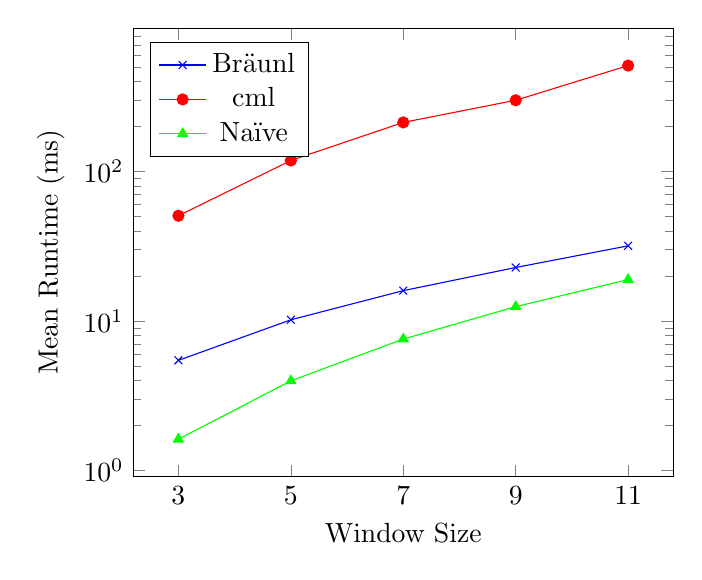
\begin{tikzpicture}
\begin{semilogyaxis}[
	xlabel=Window Size,
    ylabel=Mean Runtime (ms),
    legend pos=north west,
    %xmin=3,
    %xmax=11,
    %minor x tick num=2,
    xtick=data
]
	\addplot [mark=x,blue] table [x=windowSize,y=Mean]{
    	Method	windowSize	filename	Mean	Error	StdDev	Median	Min	Scaled	ScaledSD	Gen0	Gen1	Gen2	Allocated
Bräunl	3	very-small	5.462	0.109	0.285	5.461	4.696	3.37	0.17	31.25	15.625	15.625	2.11
Bräunl	5	very-small	10.195	0.202	0.543	10.087	9.467	2.56	0.14	46.875	31.25	15.625	3.52
Bräunl	7	very-small	15.973	0.318	0.724	15.830	15.012	2.11	0.09	46.875	15.625	-	6.04
Bräunl	9	very-small	22.807	0.447	0.829	22.497	21.855	1.83	0.07	93.75	31.25	-	9.86
Bräunl	11	very-small	31.843	0.621	0.891	31.955	29.750	1.68	0.05	187.5	62.5	-	15.63


    };
    \addplot [mark=*,red] table [x=windowSize,y=Mean]{
    	Method	windowSize	filename	Mean	Error	StdDev	Median	Min	Scaled	ScaledSD	Gen0	Gen1	Gen2	Allocated
\gls{cml}	3	very-small	50.588	2.544	7.500	49.480	40.127	31.18	4.6	166.6667	83.3333	-	1.68
\gls{cml}	5	very-small	118.463	2.349	3.443	119.399	106.345	29.75	0.99	400	200	-	1.69
\gls{cml}	7	very-small	212.817	7.252	21.270	220.862	152.973	28.08	2.79	1000	-	-	1.73
\gls{cml}	9	very-small	299.339	5.264	4.396	298.044	296.011	23.98	0.34	2000	1000	-	1.83
\gls{cml}	11	very-small	510.526	10.065	9.414	510.343	489.584	26.97	0.51	3000	1000	-	1.85

    };
    \addplot [mark=triangle*,green] table [x=windowSize,y=Mean]{
    	Method	windowSize	filename	Mean	Error	StdDev	Median	Min	Scaled	ScaledSD	Gen0	Gen1	Gen2	Allocated
Naïve	3	very-small	1.623	0.003	0.003	1.623	1.618	1	0	154.2969	35.1563	-	2.35
Naïve	5	very-small	3.983	0.076	0.071	3.980	3.891	1	0	382.8125	85.9375	-	5.62
Naïve	7	very-small	7.578	0.011	0.009	7.575	7.566	1	0	734.375	164.0625	-	10.52
Naïve	9	very-small	12.483	0.025	0.022	12.483	12.445	1	0	1171.875	203.125	-	17.26
Naïve	11	very-small	18.933	0.123	0.115	18.896	18.823	1	0	1718.75	187.5	-	23.9
    };
    
    \legend{Bräunl,\gls{cml},Naïve}
\end{semilogyaxis}
\end{tikzpicture}
\caption{\label{graph:median:verysmall}Plot of mean runtimes with a logarithmic y axis for the very small size image}
\end{figure}

%peppers
\begin{figure}
\centering
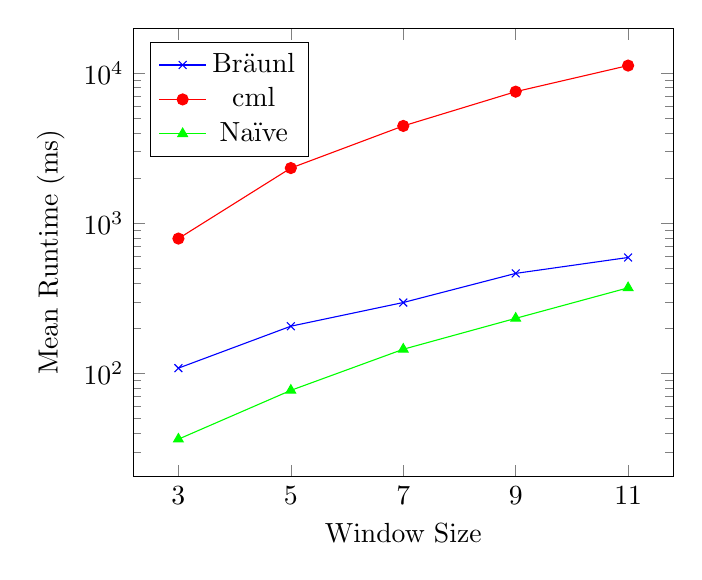
\begin{tikzpicture}
\begin{semilogyaxis}[
	xlabel=Window Size,
    ylabel=Mean Runtime (ms),
    legend pos=north west,
    %xmin=3,
    %xmax=11,
    %minor x tick num=2,
    xtick=data
]
	\addplot [mark=x,blue] table [x=windowSize,y=Mean]{
    	Method	windowSize	filename	Mean	Error	StdDev	Median	Min	Scaled	ScaledSD	Gen0	Gen1	Gen2	Allocated
Bräunl	3	peppers_gray	108.436	2.141	5.088	108.817	93.931	2.98	0.18	1200	1000	1000	37.73
Bräunl	5	peppers_gray	206.336	4.112	9.693	205.430	187.900	2.68	0.15	1000	666.6667	666.6667	58.64
Bräunl	7	peppers_gray	296.717	5.718	5.616	297.432	286.169	2.05	0.12	2000	1000	1000	114.81
Bräunl	9	peppers_gray	463.857	9.138	8.975	464.704	449.199	2	0.13	3000	2000	1000	127.86
Bräunl	11	peppers_gray	592.056	11.749	21.483	589.079	557.281	1.62	0.21	5000	2000	1000	212.34

    };
    \addplot [mark=*,red] table [x=windowSize,y=Mean]{
    	Method	windowSize	filename	Mean	Error	StdDev	Median	Min	Scaled	ScaledSD	Gen0	Gen1	Gen2	Allocated
\gls{cml}	3	peppers_gray	791.285	15.397	23.971	791.190	749.316	21.73	1.09	4000	2000	1000	28.14
\gls{cml}	5	peppers_gray	2333.317	46.639	79.197	2339.807	2108.572	30.29	1.42	8000	3000	2000	28.67
\gls{cml}	7	peppers_gray	4452.903	88.038	183.769	4407.427	4177.586	30.83	2.09	14000	5000	2000	28.28
\gls{cml}	9	peppers_gray	7533.048	150.341	225.023	7527.491	7100.467	32.49	2.2	21000	7000	2000	28.29
\gls{cml}	11	peppers_gray	11237.458	192.938	180.475	11266.773	10925.938	30.74	3.81	32000	10000	4000	29.38
    };
    \addplot [mark=triangle*,green] table [x=windowSize,y=Mean]{
    	Method	windowSize	filename	Mean	Error	StdDev	Median	Min	Scaled	ScaledSD	Gen0	Gen1	Gen2	Allocated
Naïve	3	peppers_gray	36.474	0.724	1.495	36.450	33.341	1	0	3357.1429	1000	1000	36.94
Naïve	5	peppers_gray	77.122	1.532	2.602	77.005	71.833	1	0	7285.7143	1000	1000	87.78
Naïve	7	peppers_gray	144.854	2.895	8.119	142.671	132.158	1	0	13750	1000	1000	175.21
Naïve	9	peppers_gray	232.750	5.198	15.245	227.335	213.438	1	0	21666.6667	1666.6667	1000	239.09
Naïve	11	peppers_gray	371.789	17.122	50.485	345.788	313.159	1	0	32000	1000	1000	337.86
    };
    
    \legend{Bräunl,\gls{cml},Naïve}
\end{semilogyaxis}
\end{tikzpicture}
\caption{\label{graph:median:peppers}Plot of mean runtimes with a logarithmic y axis for the peppers image}
\end{figure}

%small
\begin{figure}
\centering
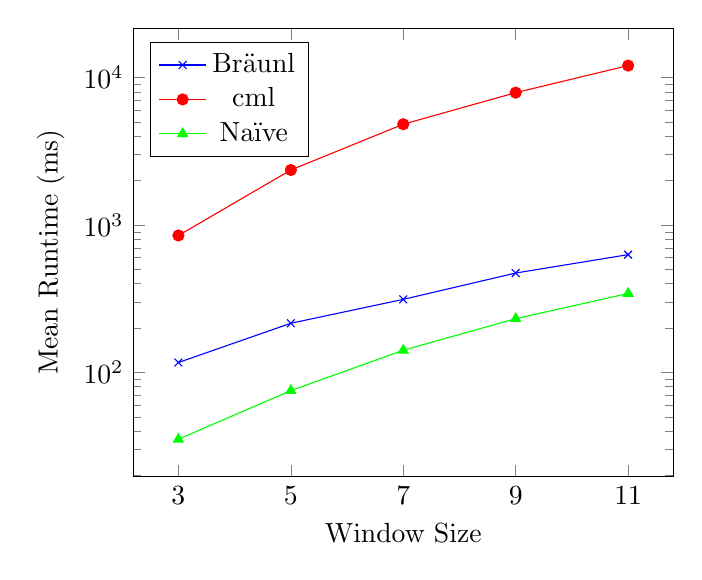
\begin{tikzpicture}
\begin{semilogyaxis}[
	xlabel=Window Size,
    ylabel=Mean Runtime (ms),
    legend pos=north west,
    %xmin=3,
    %xmax=11,
    %minor x tick num=2,
    xtick=data
]
	\addplot [mark=x,blue] table [x=windowSize,y=Mean]{
    	Method	windowSize	filename	Mean	Error	StdDev	Median	Min	Scaled	ScaledSD	Gen0	Gen1	Gen2	Allocated
Bräunl	3	small	116.782	2.334	4.208	116.874	107.437	3.32	0.14	1200	1000	800	40.96
Bräunl	5	small	215.573	4.295	12.185	217.475	180.880	2.86	0.16	1666.6667	1333.3333	1000	63.03
Bräunl	7	small	313.114	2.952	2.761	312.674	309.410	2.21	0.02	2000	1000	1000	111.37
Bräunl	9	small	472.517	4.680	4.378	473.456	460.456	2.04	0.02	4000	2000	1000	161.63
Bräunl	11	small	629.898	5.558	4.927	628.729	618.231	1.83	0.02	5000	2000	1000	149.05

    };
    \addplot [mark=*,red] table [x=windowSize,y=Mean]{
    	Method	windowSize	filename	Mean	Error	StdDev	Median	Min	Scaled	ScaledSD	Gen0	Gen1	Gen2	Allocated
\gls{cml}	3	small	849.482	19.570	56.149	828.209	773.390	24.12	1.69	4000	2000	1000	33.68
\gls{cml}	5	small	2362.643	46.461	104.871	2355.982	2162.910	31.39	1.39	9000	3000	2000	33.25
\gls{cml}	7	small	4830.294	95.856	137.474	4834.632	4523.971	34.15	0.97	14000	5000	2000	33.04
\gls{cml}	9	small	7910.925	134.530	125.839	7909.106	7701.102	34.15	0.54	23000	8000	3000	34.13
\gls{cml}	11	small	12074.170	232.388	228.236	12042.342	11712.425	35.17	0.66	32000	11000	3000	34

    };
    \addplot [mark=triangle*,green] table [x=windowSize,y=Mean]{
    	Method	windowSize	filename	Mean	Error	StdDev	Median	Min	Scaled	ScaledSD	Gen0	Gen1	Gen2	Allocated
Naïve	3	small	35.246	0.697	0.881	34.905	34.267	1	0	3466.6667	1000	1000	37.65
Naïve	5	small	75.282	0.506	0.473	75.217	74.419	1	0	7857.1429	1000	1000	95.36
Naïve	7	small	141.432	0.804	0.752	141.446	140.203	1	0	14000	1000	1000	175.74
Naïve	9	small	231.667	0.979	0.867	232.029	229.561	1	0	22666.6667	1666.6667	1000	328.08
Naïve	11	small	343.286	1.710	1.600	342.643	341.541	1	0	33000	1000	1000	261.29
    };
    
    \legend{Bräunl,\gls{cml},Naïve}
\end{semilogyaxis}
\end{tikzpicture}
\caption{\label{graph:median:small}Plot of mean runtimes with a logarithmic y axis for the small size image}
\end{figure}

\begin{anfxerror}
Really need to change these charts to use a log scale on the y axis.  It'll make it much easier to see the relative changes.
\end{anfxerror}

%medium
\begin{figure}
\centering
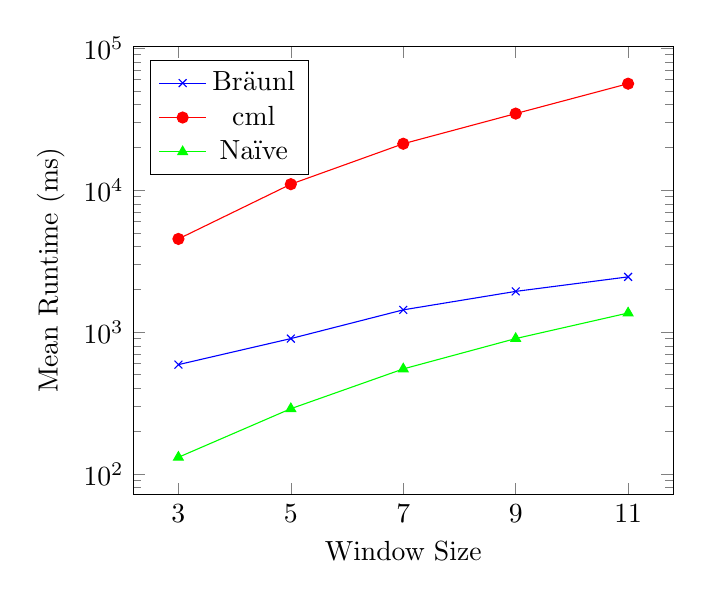
\begin{tikzpicture}
\begin{semilogyaxis}[
	xlabel=Window Size,
    ylabel=Mean Runtime (ms),
    legend pos=north west,
    %xmin=3,
    %xmax=11,
    %minor x tick num=2,
    xtick=data
]
	\addplot [mark=x,blue] table [x=windowSize,y=Mean]{
    	Method	windowSize	filename	Mean	Error	StdDev	Median	Min	Scaled	ScaledSD	Gen0	Gen1	Gen2	Allocated
Bräunl	3	medium	589.431	11.668	10.344	585.135	574.774	4.51	0.27	2000	1000	1000	146.49
Bräunl	5	medium	899.233	4.445	3.940	899.270	892.109	3.12	0.07	4000	2000	1000	230.3
Bräunl	7	medium	1433.220	31.164	29.151	1431.262	1379.761	2.61	0.07	7000	4000	2000	374.04
Bräunl	9	medium	1933.758	24.222	22.657	1925.642	1905.768	2.15	0.02	16000	4000	2000	527.35
Bräunl	11	medium	2447.284	47.271	50.580	2451.473	2352.536	1.8	0.05	40000	4000	2000	167.19

    };
    \addplot [mark=*,red] table [x=windowSize,y=Mean]{
    	Method	windowSize	filename	Mean	Error	StdDev	Median	Min	Scaled	ScaledSD	Gen0	Gen1	Gen2	Allocated
\gls{cml}	3	medium	4527.962	89.754	226.819	4511.961	4003.316	34.65	2.61	12000	6000	3000	132.41
\gls{cml}	5	medium	11006.775	197.445	184.691	10983.829	10737.131	38.19	1.05	28000	10000	4000	138.84
\gls{cml}	7	medium	21210.296	417.303	409.847	21118.240	20410.160	38.61	1.08	50000	15000	4000	136.78
\gls{cml}	9	medium	34587.347	471.655	441.186	34687.611	33898.247	38.45	0.48	81000	22000	4000	137.63
\gls{cml}	11	medium	56196.611	1118.853	2548.193	55158.372	52956.449	41.29	2.05	230000	66000	4000	132.75
    };
    \addplot [mark=triangle*,green] table [x=windowSize,y=Mean]{
    	Method	windowSize	filename	Mean	Error	StdDev	Median	Min	Scaled	ScaledSD	Gen0	Gen1	Gen2	Allocated
Naïve	3	medium	131.111	2.655	7.787	128.188	122.294	1	0	11500	1500	1500	102.34
Naïve	5	medium	288.343	5.716	6.805	285.656	282.623	1	0	28000	1000	1000	371.43
Naïve	7	medium	549.600	12.951	12.114	543.465	539.418	1	0	54000	1000	1000	710.4
Naïve	9	medium	899.563	3.131	2.444	900.523	893.992	1	0	89000	2000	1000	985.29
Naïve	11	medium	1361.629	27.108	31.217	1350.193	1344.088	1	0	131000	4000	1000	1969.78
    };
    
    \legend{Bräunl,\gls{cml},Naïve}
\end{semilogyaxis}
\end{tikzpicture}
\caption{\label{graph:median:medium}Plot of mean runtimes with a logarithmic y axis for the medium size image}
\end{figure}

%\gls{cml}
\begin{figure}
\centering
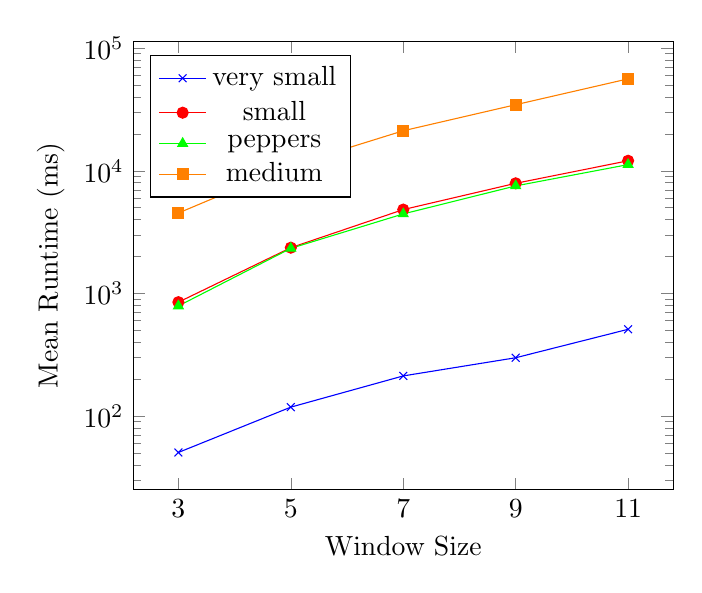
\begin{tikzpicture}
\begin{semilogyaxis}[
	xlabel=Window Size,
    ylabel=Mean Runtime (ms),
    legend pos=north west,
    %xmin=3,
    %xmax=11,
    %minor x tick num=2,
    xtick=data
]
	\addplot [mark=x,blue] table [x=windowSize,y=Mean]{
    	Method	windowSize	filename	Mean	Error	StdDev	Median	Min	Scaled	ScaledSD	Gen0	Gen1	Gen2	Allocated
\gls{cml}	3	very-small	50.588	2.544	7.500	49.480	40.127	31.18	4.6	166.6667	83.3333	-	1.68
\gls{cml}	5	very-small	118.463	2.349	3.443	119.399	106.345	29.75	0.99	400	200	-	1.69
\gls{cml}	7	very-small	212.817	7.252	21.270	220.862	152.973	28.08	2.79	1000	-	-	1.73
\gls{cml}	9	very-small	299.339	5.264	4.396	298.044	296.011	23.98	0.34	2000	1000	-	1.83
\gls{cml}	11	very-small	510.526	10.065	9.414	510.343	489.584	26.97	0.51	3000	1000	-	1.85


    };
    \addplot [mark=*,red] table [x=windowSize,y=Mean]{
    	Method	windowSize	filename	Mean	Error	StdDev	Median	Min	Scaled	ScaledSD	Gen0	Gen1	Gen2	Allocated
\gls{cml}	3	small	849.482	19.570	56.149	828.209	773.390	24.12	1.69	4000	2000	1000	33.68
\gls{cml}	5	small	2362.643	46.461	104.871	2355.982	2162.910	31.39	1.39	9000	3000	2000	33.25
\gls{cml}	7	small	4830.294	95.856	137.474	4834.632	4523.971	34.15	0.97	14000	5000	2000	33.04
\gls{cml}	9	small	7910.925	134.530	125.839	7909.106	7701.102	34.15	0.54	23000	8000	3000	34.13
\gls{cml}	11	small	12074.170	232.388	228.236	12042.342	11712.425	35.17	0.66	32000	11000	3000	34

    };
    \addplot [mark=triangle*,green] table [x=windowSize,y=Mean]{
    	Method	windowSize	filename	Mean	Error	StdDev	Median	Min	Scaled	ScaledSD	Gen0	Gen1	Gen2	Allocated
\gls{cml}	3	peppers_gray	791.285	15.397	23.971	791.190	749.316	21.73	1.09	4000	2000	1000	28.14
\gls{cml}	5	peppers_gray	2333.317	46.639	79.197	2339.807	2108.572	30.29	1.42	8000	3000	2000	28.67
\gls{cml}	7	peppers_gray	4452.903	88.038	183.769	4407.427	4177.586	30.83	2.09	14000	5000	2000	28.28
\gls{cml}	9	peppers_gray	7533.048	150.341	225.023	7527.491	7100.467	32.49	2.2	21000	7000	2000	28.29
\gls{cml}	11	peppers_gray	11237.458	192.938	180.475	11266.773	10925.938	30.74	3.81	32000	10000	4000	29.38
    };
    \addplot [mark=square*,orange] table [x=windowSize,y=Mean]{
    	Method	windowSize	filename	Mean	Error	StdDev	Median	Min	Scaled	ScaledSD	Gen0	Gen1	Gen2	Allocated
\gls{cml}	3	medium	4527.962	89.754	226.819	4511.961	4003.316	34.65	2.61	12000	6000	3000	132.41
\gls{cml}	5	medium	11006.775	197.445	184.691	10983.829	10737.131	38.19	1.05	28000	10000	4000	138.84
\gls{cml}	7	medium	21210.296	417.303	409.847	21118.240	20410.160	38.61	1.08	50000	15000	4000	136.78
\gls{cml}	9	medium	34587.347	471.655	441.186	34687.611	33898.247	38.45	0.48	81000	22000	4000	137.63
\gls{cml}	11	medium	56196.611	1118.853	2548.193	55158.372	52956.449	41.29	2.05	230000	66000	4000	132.75
    };
    
    \legend{very small,small,peppers,medium}
\end{semilogyaxis}
\end{tikzpicture}
\caption[Plot of mean runtimes for the \glsentrylong{cml-glossary} algorithm on different image sizes]{\label{graph:median:cmls}Plot of mean runtimes with a logarithmic y axis for the \gls{cml} algorithm on different image sizes}
\end{figure}

\begin{figure*}
\subfloat[]{\includegraphics[width=0.2\textwidth]{chapters/medianfilter/images/peppers/peppers_gray.png}}
\subfloat[]{\includegraphics[width=0.2\textwidth]{chapters/medianfilter/images/peppers/peppers_gray_noisy.png}}
\subfloat[]{\includegraphics[width=0.2\textwidth]{chapters/medianfilter/images/peppers/naive_peppers_gray_noisy_3.png}}
\subfloat[]{\includegraphics[width=0.2\textwidth]{chapters/medianfilter/images/peppers/braunl_peppers_gray_noisy_3.png}}
\subfloat[]{\includegraphics[width=0.2\textwidth]{chapters/medianfilter/images/peppers/cml_peppers_gray_noisy_3.png}}
\caption[The classic grayscale `peppers' image, before and after processing]{\label{fig:median:peppers}The classic grayscale `peppers' image, before and after processing.  (a) is the original image; (b) is the image with random salt \& pepper noise introduced; (c) is the result of processing the image using the naïve algorithm; (d) is the result of processing the image using the Br\"{a}unl-inspired algorithm; (e) is the result of processing the image using the \gls{cml} algorithm}
\end{figure*}

\begin{table}
\centering
\caption[Peak signal-to-noise for the very small image]{Peak signal-to-noise ratio measurement for the very small image (measured in dB)}
\label{tab:median:psnrvsmall}
\begin{tabular}{@{}lccccc@{}}
\toprule
\multicolumn{1}{c}{\textbf{Algorithm}} & \multicolumn{5}{c}{\textbf{Window size}}                                          \\
                                       & 3              & 5              & 7              & 9             & 11             \\ \midrule
Bräunl                                 & 20.78          & 17.82          & 15.65          & 14.36         & 13.55          \\
\gls{cml}                                    & 25.98          & \textbf{21.85} & \textbf{18.62} & \textbf{16.40} & 14.99          \\
Naïve                                  & \textbf{27.03} & 21.74          & 18.55          & 16.39         & \textbf{15.02} \\ \bottomrule
\end{tabular}
\end{table}

\begin{table}
\centering
\caption[Peak signal-to-noise for the peppers image]{Peak signal-to-noise ratio measurement for the peppers image (measured in dB)}
\begin{tabular}{@{}lccccc@{}}
\toprule
\multicolumn{1}{c}{\textbf{Algorithm}} & \multicolumn{5}{c}{\textbf{Window size}}                                          \\
                                       & 3              & 5              & 7              & 9              & 11            \\ \midrule
Bräunl                                 & 28.76          & 27.35          & 25.27          & 23.94          & 22.82         \\
\gls{cml}                                    & 31.85          & 31.07          & 29.8           & 28.56          & 27.42         \\
Naïve                                  & \textbf{32.79} & \textbf{31.25} & \textbf{29.87} & \textbf{28.63} & \textbf{27.50} \\ \bottomrule
\end{tabular}
\label{tab:median:psnrpeppers}
\end{table}

\begin{table}
\centering
\caption[Peak signal-to-noise for the small image]{Peak signal-to-noise ratio measurement for the small image (measured in dB)}
\label{tab:median:psnrsmall}
\begin{tabular}{@{}lccccc@{}}
\toprule
\multicolumn{1}{c}{\textbf{Algorithm}} & \multicolumn{5}{c}{\textbf{Window size}}                                          \\
                                       & 3              & 5              & 7             & 9              & 11             \\ \midrule
Bräunl                                 & 32.83          & 32.34          & 30.74         & 29.73          & 28.94          \\
\gls{cml}                                    & 36.62          & 34.25          & 32.66         & 31.57          & 30.71          \\
Naïve                                  & \textbf{37.83} & \textbf{34.31} & \textbf{32.7} & \textbf{31.65} & \textbf{30.81} \\ \bottomrule
\end{tabular}
\end{table}

\begin{table}
\centering
\caption[Peak signal-to-noise for the medium image]{Peak signal-to-noise ratio measurement for the medium image (measured in dB)}
\begin{tabular}{@{}lccccc@{}}
\toprule
\multicolumn{1}{c}{\textbf{Algorithm}} & \multicolumn{5}{c}{\textbf{Window size}}                                           \\
                                       & 3              & 5              & 7              & 9              & 11             \\ \midrule
Bräunl                                 & 32.98          & 32.65          & 31.59          & 30.91          & 30.36          \\
\gls{cml}                                    & 36.72          & \textbf{34.15} & \textbf{32.98} & \textbf{32.26} & \textbf{31.73} \\
Naïve                                  & \textbf{37.16} & 34.07          & 32.96          & \textbf{32.26} & \textbf{31.73} \\ \bottomrule
\end{tabular}
\label{tab:median:psnrmedium}
\end{table}

Examination of the reported memory statistics (please see the GitHub repository for details) appears to show that the maximum amount of memory allocated during processing for the \gls{cml} algorithm stays roughly constant across window sizes for each image size, and in fact on larger window sizes it is the most memory efficient.  The naïve algorithm quickly grows to consume the most memory at larger window sizes for each image size, suggesting that it likely derives some of its comparative speed at the cost of greater space complexity, while Bräunl sits in the middle.  Conversely, \gls{cml} generates by far the most garbage collection events, which may help explain its relative lack of pace.

\section{Discussion}
%These algorithms are not necessarily the best for performing this operation, as they ignore the potential for taking advantage of data-parallelism.

The algorithms developed and presented here are not necessarily optimal for the purpose.  They largely handle each pixel separately, or combine them into arrays on-the-fly.  This ignores the possibility of exploiting data-parallelism to improve throughput, and instead relies only on the separate CPU cores to provide the parallelism.

It is unclear how much the mechanics underlying these implementations (i.e. the .NET Core and \hopac{} systems) attempt to maximise use of the processor cache.  Efficient use of the cache can contribute significantly to an optimised version of an algorithm outperforming a simplistic version by an order of magnitude or more \cite{Ragan-Kelley2017}.  No attempt was made manually to ensure good practices such as tiling or striping.  %Differences in cache exploitation may also go some way to explaining differences in execution time.

The \gls{cml} approach used essentially instantiates a separate logical processing element for each pixel, each of which must be scheduled to run at some point -- concurrent with another one in the case of synchronous message passing.  It is possible that this surfeit of separate logical threads may induce excessive switching costs, and perhaps promote wasted time with threads spending time polling their channel and their neighbours'.  Careful improvements to this and the use of the cache might lead to significant gains in speed.

In terms of the code itself also, \gls{cml} appears to be the worst.  The program requires roughly double the number of lines of the naïve program, and is arguably much less `clean' or `readable'.  Reinterpreting the \gls{medianfilter} in terms of synchronously communicating processes has not yielded a structural improvement nor simplified the programming task.  Combined with the running time results above, this suggests that the \gls{cml} approach is actively unhelpful for implementing \glspl{mwt}, at least when using \hopac{}.

Basic profiling of the \gls{cml}-based implementation appears to show that more than half of the runtime of the program was spent inside the function for giving a value over a channel, and functions called by it.  Furthermore, according to this profiling, almost 40\% of the total running time of the algorithm is taken up specifically by low-level memory management functions inside the depths of the .NET Core system.  Considering that some of these functions are written in hand-optimised assembly \fxwarning[inline]{ref?}, the fact they account for so much of the running time appears to suggest that memory use is poorly handled in the tested implementation.

\Glspl{mwt} are generally relatively simplistic processes, which typically consist simply of combining values from the pixel array, which can be programmed in a straightforward fashion.  More sophisticated programming techniques may simply `get in the way' and introduce unnecessary overheads, which appears to have happened here.  Furthermore, the \gls{medianfilter} can largely be broken down into arithmetic and logical operations amenable to vectorisation (e.g. \cite{Sanchez2012,Perreault2007}), which the \gls{cml} approach currently ignores entirely.

\subsection{Threats to validity}
There are two identifiable threats to validity, both regarding the `quality' of the programming involved.  .NET Core, as a widely used open source compiler and runtime system which has likely had millions of man-hours invested in it, is presumably of high quality and fast in most cases.  That is not necessarily the case with \hopac{}.  While it is open source, and moderately well-known in the \fsharp{} community, the amount of time spent on optimising it is likely nowhere close to that spent on .NET Core.  This means that \hopac{} itself may present significant bottlenecks while performing the \gls{mwt}.  While it is reasonable to expect that `give' operations would be a large part of the total running time, as a central part of the operation of the algorithm, it is surprising to see it take more than 50\% of the time.

The other threat to validity is the skill of the end programmer.  The author was new to the \hopac{} library at the start of this work, and inferior design choices may have been made unwittingly.  It was, however, suggested during personal communication with one of the maintainers and fellow users of the \hopac{} library that the \gls{cml} approach may simply be a poor fit to pixel-wise image processing tasks.

Fundamentally, the results achieved here, as with most implementation exercises, succeed or fail in large part on the skill, knowledge and effort of the programmers involved.  The use of other libraries may lead to better results.  Other relatively recent implementations of \gls{cml} exist, such as Concurrent Haskell \cite{Chaudhuri2009} and Fibers\footnote{\url{https://github.com/wingo/fibers}} for Guile Scheme, but a lack of time meant that they could not yet be assessed further.

\section{Conclusion}
The use of a \gls{cml} approach to image processing was explored in this work, in particular as applied to the \gls{medianfilter} \gls{mwt} operation.  The measured results suggest that it is much worse than using a simple, naïve nested-for-loops approach.  The reason for this appears to be primarily related to overhead from the synchronous communications, especially in regard to memory allocations and garbage collections.  This may be an issue with the \gls{cml} style in general, \fxerror{That ended up looking like it was at least partially true.}{or it may be an issue related to the \gls{cml} library used} or the programming of the algorithms tested here.  More work is required to determine this for certain.  \gls{cml} does appear to provide one advantage, however, in that for larger window sizes it seemingly has the lowest peak space requirement.

A \gls{cml} approach where a separate logical processing element is used to represent each pixel largely eliminates the possibility of taking advantage of data-parallel hardware, such as vector instructions of CPUs or \glspl{gpu}.  For situations where vector instructions are applicable, the \gls{cml} approach seems likely to be a poor choice.  It is not clear, however, how well this approach may or may not work for instances where the data types involved are more complex, or where there is a significant level of control flow involved.

% Future work should explore \gls{cml} as applied to other computer vision algorithms, especially those which can naturally be characterised in terms of message passing, or which use more complex data types.  Other \gls{cml} implementations beyond the one used here should be tested too, as it is not clear how much the problems experienced by this \gls{cml} program may stem from the implementation of the \gls{cml} library used.
% \glsresetall
% \cpresetrulenumber
% \chapter{Discussion}

Where I discuss the good \& bad about this work

% \section{Comparison of \glsentrylong{mpbsm} algorithms}

% What am I comparing them to?  Algos coded by myself?  The best I can find out there of others'?

% \subsection{\glsentrylong{bp}}

% \subsection{\glsentrylong{cp}}

\section{Limitations}

\subsection{Threats to Validity}

\section{Alternatives for Investigation}

\subsection{Other languages \& libraries}
Implement my own version of \gls{cml} in Rust or Julia, etc?  Looks like Felix has most if not all of the necessary components for it.

\subsection{Other Computational Models}
Actors, Join Calculus, Pi Calculus

\subsection{Potentially Useful Hardware}

\subsubsection{CPU Additions}
Intel's Transactional Synchronisation Extensions (TSX) -- \url{https://en.wikipedia.org/wiki/Transactional_Synchronization_Extensions}

AMD's Advanced Synchronization Facility (ASF) -- \url{https://en.wikipedia.org/wiki/Advanced_Synchronization_Facility}

mEDA (modified Extended Dataflow Actor) \& full/empty memory tagging (F/E bits?) e.g. \url{https://link.springer.com/chapter/10.1007/BFb0057916} \& \url{https://people.kth.se/~vladv/abstracts/TRITA-IT-0004.pdf}

\subsubsection{Is Hyper-Threading Helpful?}

\subsubsection{GPUs?}

% \glsresetall
% \cpresetrulenumber
% \chapter{Conclusion}

I did some stuff!

\section{Future Directions}

\begin{anfxwarning}{Where should this go?}
    Similar material is also covered in the discussion chapter.  Should much of the below be shifted into there?  Alternatively, should much of the stuff from the discussion chapter move to here?
\end{anfxwarning}

% The use of Full/Empty bits looks highly promising for making message passing more efficient.  It doesn't seem to have any real support in mainstream/commodity hardware, however.  There were Intel's TGX instructions, but they have been taken out of processors again.

% Extended Dataflow Actors?  Or is it Extended Dataflow Architecture?

% \fxerror*{Not entirely sure BSP is relevant here}{See also the Bulk Synchronous Parallel approach.}

% https://scholar.google.co.nz/scholar?q=related:Z8GZl-HQcSkJ:scholar.google.com/&scioq=A+Static+Mapping+System+for+Logically+Shared+Memory+Parallel+Programs&hl=en&as_sdt=0,5&inst=15360723290749679499

% http://citeseerx.ist.psu.edu/viewdoc/download?doi=10.1.1.50.8739&rep=rep1&type=pdf

% https://link.springer.com/chapter/10.1007/BFb0057916

% https://link.springer.com/chapter/10.1007/3-540-63697-8_82

None of the below were investigated further, due to a lack of time, but they are obvious next steps to look at.

% \subsection{\glsentrytext{cml}}
% \Gls{cml} seems like the obvious approach to take from here.\footnote{In fact, considerable time and effort was spent on attempting to identify a suitable \gls{cml} implementation to use for just this purpose.  Unfortunately, in the end, it was found that there was not currently a usable \gls{cml} implementation with appropriate performance available at this time.}

% \subsection{`Faked' message passing in shared memory}
% Roughly, most of the message passing involved here is largely, in effect, just handing around pointers to memory locations.  It would seem that the message passing itself places some overhead in the way of that.  Could there be some way to fake the message passing, so that to the program's writer it looks like an actual message passing implementation, but in reality it is just doing normal updates on mutable memory?  This \emph{might} enable the best of both worlds -- programming the algorithms according to their theory, but running in a highly efficient fashion `under-the-hood'.

% It is not too clear how to achieve this (if it is indeed possible), but Rust would appear to be a good language to target for it.  Rust is fairly high-performance by default and enables quite a lot of low-level memory manipulation.  Moreover, its move semantics pretty much fit exactly to the concepts used here, and, on the face of it, its macro system would appear to be a convenient way to abstract over many of the details and provide a message passing façade, while actually doing efficient operations behind that.

% It looks like the C++ \texttt{mess} library is intended to be exactly this sort of thing:  \url{https://github.com/LouisCharlesC/mess}.  The developer seems to say that the user gets to write their program in a message-passing fashion, but mess does some clever meta-programming so that there ends up being zero overhead in the end.  Also, absolutely \emph{must} address Halide, and explain why it wasn't pursued here.  Otherwise, that'll be the elephant in the room.

% \subsection{Other hardware}
% This work focused on CPU-based systems, largely excluding other hardware.  If used well, all three of \glspl{gpu}, \glspl{fpga} and \glspl{dsp} have potential to perform vastly more computations per second, suggesting that a high-performance message passing-based system would do well to use them.  In each case, however, they do not work in quite the same way as CPUs, meaning that programming them is not necessarily straightforward, especially when trying to achieve a programming style that differs to their default.  As described in \fxwarning*{insert the appropriate cross-reference}{the literature review chapter}, fast \gls{gpu} implementations of \gls{bp} have been created, suggesting that message passing on a \gls{gpu} is entirely plausible.

% It would appear worthwhile to investigate how one might be able to implement some sort of message passing system atop these hardware alternatives, due to the potential for many more computations per second.  Even better would be to create a heterogeneous system which can take full advantage of the strengths of each hardware type, while overcoming its weaknesses.  Precisely how to achieve efficient implementations on them is unknown.  The fact that OpenCL \fxerror[inline]{[ref]} (and, to some extent at least, OpenACC \fxerror[inline]{[ref]}) can be compiled from the same base code to different devices makes it an obvious starting point.   There has already been at least one publication on implementing \glspl{actor} in OpenCL \fxerror[inline]{[ref]}, suggesting it is possible -- though how well synchronous message passing will work as compared to asynchronous remains to be seen.

% See also \url{https://hastlayer.com/} -- they seem to say that they do relevant stuff on FPGAs.  Interestingly, they also do unums/posits, apparently.

\subsection{Universal Numbers}
The \gls{cps} work kinda ignored non-integer numbers, which in real practice is quite a glaring omission.  Investigating modelling IEEE-754 floating point (and/or the fixed-point version), as well as Gufstafson's unums/posits, would be another good step to take.

%%%%%%%%%%%%%%%%%%%%%%%%%%%%%%%%%%%%%%%%%%%%%%%%%%%%%%%%%%%%%%%%%%%%%%%%%%%%%%%%%

\subsection{\nameref{chap:tsp}}
One-way multiset unification occurs frequently in \gls{cps}, with unification being used in every rule presented above.  \fxerror*{Isn't this what Yezhou's paper \cite{Liu2021} covers?}{An efficient algorithm to perform this task would be highly beneficial for creating useful simulations of systems (we are not aware of an efficient algorithm in the case of multisets).}  For example, our simulations of the \gls{tsp} algorithm written in functional programming languages (see \cref{sec:tsp:simulation}) regularly simply iterate over all relevant objects in the system, even though frequently most will be of little use in a given function call, and so the simulations could benefit from improved unification in practice.

We would like to further develop the capacity to simulate \gls{cps}, in particular developing more advanced techniques for translating \gls{cps} rules to efficient parallel code.  Work down this avenue has not begun as yet, however.

%%%%%%%%%%%%%%%%%%%%%%%%%%%%%%%%%%%%%%%%%%%%%%%%%%%%%%%%%%%%%%%%%%%%%%%%%%%%%%%%%

\subsection{\nameref{chap:median}}

The median filter algorithm investigated was pretty much the most basic one possible.  The experiment should be extended to cover more complicated algorithms that perform better at reconstructing the image.  These may be better suited to a message-passing approach compared to a na\"ive one than the basic method.

Future work should explore \gls{cml} as applied to other computer vision algorithms, especially those which can naturally be characterised in terms of message passing, or which use more complex data types.  Other \gls{cml} implementations beyond the one used here should be tested too, as it is not clear how much the problems experienced by this \gls{cml} program may stem from the implementation of the \gls{cml} library used.

%%%%%%%%%%%%%%%%%%%%%%%%%%%%%%%%%%%%%%%%%%%%%%%%%%%%%%%%%%%%%%%%%%%%%%%%%%%%%%%%%

\subsection{\nameref{chap:nmp}}
The next step in this work is to adapt the system to the purpose of Belief Propagation Stereo Matching, using \gls{nmp} precepts.  This will be presented in Part Two.  Furthermore, work has begun on implementing a close approximation of the asynchronous system as a framework in a standard programming languages, to explore the effectiveness of this approach in modern computer systems.  We plan to implement Belief Propagation Stereo Matching (see e.g. \cite{Blake2011,Felzenszwalb2011,JianSun2003}) atop this as a proof-of-concept.

One aspect the systems presented above lack is that both the size and shape of the grid involved, as well as the communication topology between neighbours, are permanently fixed at the time of system initialisation.  In most cases, this is unneeded, but the greater flexibility could be of use when implementing certain algorithms.

Furthermore, at present, it is implicitly assumed that every \gls{pe} remains active throughout the entirety of the system's evolution until it has sent and received all of its scheduled messages.  Within the context of \gls{cps} this is largely irrelevant, but permitting \glspl{pe} to deactivate at appropriate points could save processing power in other circumstances with bounded parallelism.  Complicating this is ensuring that those \glspl{pe} which do remain active can continue messaging as needed despite one or more neighbours deactivating.

We also have yet to examine the systems with respect to communication complexity measures such as those found in \cite{Juayong2020}.  The precise results presented there are not directly applicable to this work, given the use of different P~systems models, but the underlying concepts appear directly relevant.

%%%%%%%%%%%%%%%%%%%%%%%%%%%%%%%%%%%%%%%%%%%%%%%%%%%%%%%%%%%%%%%%%%%%%%%%%%%%%%%%%

\chapter{Introduction}
Some wordiness will go here.

\section{My first section}
Post-introductory wordiness

Main goal:  To achieve at least one of the below
\begin{itemize}
\item run more efficiently (faster and/or use less memory)
\item Scalability.  If one only scales well up to, say 4-8 cores, but the other works up to a much larger number of cores, then that would suggest that the latter approach is much more future-proof, since best guesses still suggest that manycore systems are the way of the future.
\item `cleaner'/nicer code (by some reasonably objective, quantifiable measure)
\item `easier to program/easier to read' -- lower complexity (how does one measure that though?)
\end{itemize}

Why is message passing better than using an algorithmic skeleton?  Or how much can the two ideas be unified?  (e.g. a \gls{cml} inspired skeleton for operations on regular grids -- perhaps using specific neighbourhoods).

Some of the stereo matching algorithms can be described in terms of message passing, but also can be given fairly efficient GPU implementations.  How do the two connect?

From \url{https://abacus.bates.edu/~ganderso/biology/resources/writing/HTWsections.html}:  ``the Introduction must answer the questions, "What was I studying? Why was it an important question? What did we know about it before I did this study? How will this study advance our knowledge?"''

\section{Research Questions}
\begin{enumerate}
    \item Can real-time message passing-based stereo matching be implemented using a message passing programming approach?
    \item How do the results compare with more traditional implementations?
    \item 
\end{enumerate}

\subsection{Research Question One}
Here real-time means achieving a speed of at least 1 frame per second, i.e. at least 1 Hz.

\subsection{Research Question Two}
Comparisons can be (will be?) made based on runtime efficiency, both with `wall time' taken and peak memory use, as well as based on code-quality measures in some fashion.  Also, if possible, check how well each approach scales.

\subsection{Research Question Three}

\section{Hypotheses}

\subsection{Hypothesis One}
On larger/more powerful systems, yes.  On smaller systems (e.g. Nvidia Jetson Nano) no.

\subsection{Hypothesis Two}
\gls{mpbsm} will be \emph{slower} than traditional methods, and use more memory.  The program will be longer, but it will be more clearly logically structured.  It will scale better than traditional approaches though, when there is shared memory but distinct processors.

\subsection{Hypothesis Three}

\section{Outline}
Where I summarise the upcoming dissertation (this section probably needs a different/better name).  Where in the intro do I explain the novelty?
\glsresetall
\cpresetrulenumber
\chapter{Background and Related Work}
\fxerror{Some of this probably should be chopped now...}{This review of related past work} focuses on the main areas of Computer Science that are relevant to this dissertation:  Formal Models of Computation (especially \gls{ps}) and \glsentrylong{cml-glossary} --- a big part of the \gls{ps} stuff is \gls{cps}, but that seemed to be big enough to merit its own chapter.  In none of these cases does the review come close to comprehensively covering the entire span of the given area.  It merely tries to cover as much of the relevant recent and classic work as possible, while giving an extremely brief introduction to these areas.  The interested reader who is unfamiliar with any of these topics is strongly advised to refer to the materials cited.

% See \url{http://forneylab.org/} for something seemingly quite similar to what I'm doing...;  fglib \url{https://github.com/danbar/fglib};  IGraph library \url{https://igraph.org/};  LGNpy \url{https://github.com/ostwalprasad/LGNpy};  

\section{Formal Models of Concurrent Computation}
Perhaps the earliest (or at least, the earliest that is still widely known) formalised model of concurrent computation is the Petri Net \cite{Dennis2011}, first conceived of by Carl Petri, initially for the purpose of describing chemical processes \cite{Petri2008}.

\begin{anfxerror}{Why not Petri Nets?}
Why are Petri Nets not more popular?  Why do we choose \gls{csp} or \glspl{actor} or \gls{ps} over them?
\end{anfxerror}

\cite{Varela2013}

This work 

\subsection{\glsentrylong{csp} \& Pi~Calculus}
\gls{csp} is a `process algebra' and abstract model of concurrent computation put forward by Hoare \cite{Hoare1985,Roscoe2011}.  A typical sequential computation is represented by a `process'.  Processes' ``behaviour is described in terms of the occurrence and availability of abstract entities called \textit{events}'' \cite[p.~478]{Roscoe2011}.  Should more than one event be available simultaneously for a given process, then one will be chosen non-deterministically.  This choice is internal to the process, and not influenced by or visible to any other process.  %E.g. for a situation where there is one possible event \(a\) at a given point in time, the process \(P\) will choose that event and then proceed according to the result, written as: \[ a \rightarrow P(a) \]

Concurrency is introduced by the existence of multiple processes.  In general, the processes evolve independently, responding to events as they come.  Should a particular event appear in the alphabet of multiple processes, however, then all processes \emph{must} choose to participate in that event at the same time.  Should all processes involved make such a choice, they engage in a synchronous multi-way atomic synchronisation (hence `communicating').  \gls{csp} has provided significant inspiration for concurrency design in a number of programming languages, notably including Ada \cite{Defense1983,Taft2013}, Occam \cite{Elizabeth1987}, Google's Go \cite{Meyerson2014} (not to be confused with the earlier language Go! \cite{Clark2004}, which itself was explicitly designed for concurrency) and \gls{cml} \cite{Reppy2011}. 

Milner appreciated \gls{csp}, which advanced concurrency models by explicitly incorporating \emph{synchronised} interaction, something Milner's earlier Calculus for Communicating Systems \cite{Milner1980} had lacked  \cite{Milner1993}.  Milner still regarded \gls{csp} as incomplete, however, in that it had no support for the concept of `mobility' -- i.e. the ability of the system to reconfigure itself during operation.  Pi Calculus was created as an attempt to build upon those earlier systems but present a complete calculus of concurrent computation in much the same way that Lambda Calculus \cite{Barendregt1984} is a complete calculus for sequential computation.\footnote{Milner also pointed out that sequential computation is, in fact, a special case of concurrent computation.}

\subsection{\label{subsec:actors}\texorpdfstring{\Glspl{actor}}{Actors}}
The \gls{actor} \cite{Agha1986} model was introduced by Hewitt \cite{Hewitt1973}.  Much like \gls{csp} \& its cousins, the \gls{actor} model is based around the concept of separated, sequential but communicating processes which exchange messages.  Again, the processes make decisions and proceed based on their communications.  A key difference, however, is that in the \gls{actor} model the message exchanges are \emph{a}synchronous.  Each \gls{actor} has its own `mailbox', and may send messages to other \glspl{actor} so long as it knows their name (which is equivalent for this purpose to a concept of an address for the \gls{actor}), \emph{but does not wait at all for a response before proceeding}.

The \gls{actor} model is a popular one for concurrent programming, possibly owing to its intuitive concept.  The fact that communication is asynchronous makes \glspl{actor} much more suitable for modelling distributed systems without shared memory than \gls{csp} or similar -- \glspl{actor} can send messages and proceed without (necessarily) needing to wait for a response, instead continuing to process based on the messages they themselves have received.  By contrast, a system with synchronous communication would have prohibitive time costs, given the relative slow speed of typical links between distributed computers as compared to their capacity for local processing.  Many \gls{actor} systems have been implemented for different programming languages (e.g. \cite{Varela2001,Srinivasan2008,Charousset2016,Bernstein2016} \fxnote[inline,nomargin]{[need more refs?]}), and in fact it is a core component, and perhaps largely responsible for the success, of Erlang/OTP \cite{Armstrong2010,Armstrong2013,Vinoski2012}.  A relatively new language, Pony \cite{Clebsch2015,Clebsch2017}, takes this even further.
\begin{anfxnote}{Positive example for actors?}
In Concurrency in .NET, Terrell described using an actor to control access to a shared resource and stated that it was an extremely effective solution.
\end{anfxnote}

\Glspl{actor}, when used for non-trivial real-world software, have been criticised at times \cite{Welsh2013,Stucchio2013}.  While some of the criticisms described are implementation-specific (relating to Akka, a Scala \gls{actor} library), a common thread is that \glspl{actor} do not compose well.  This has the negative consequence that it is difficult to combine an \gls{actor} with anything else to create a new abstraction, and can require extensive modifications in source code to make relatively simple changes.

\subsection{Join Calculus}

\begin{anfxwarning}{Join Calc refs}
Chemical abstract machine, joinads, Scala communicating objects (IIRC, that was join calculus based), reagents
\end{anfxwarning}

\subsection{Others}
Mobility calculus.  Others?

% \subsection{Criticisms}

% Gorlatch \cite{Gorlatch2004} argued against basic message passing, decrying it as an unnecessary and unhelpful complication and favouring \fxerror*{What does `collective operations' mean?}{`collective' operations} instead.  This criticism focused upon \gls{mpi} as it was at the time, however, and made no reference to either Actors or \gls{csp}. \fxerror{Does subsection this truly belong here?}

\section{\glsentrytext{ps}/\glsentrytext{mc}}
% \Gls{ps}, also known as \Gls{mc} (the two terms are generally used interchangeably), is a bio-inspired model of computing created by Gheorghe Păun in the late 1990s \cite{tPaun98a,Paun2000}.  It was originally conceived of by considering the process of chemical reactions and exchanges that occur inside living biological cells \& the membranes within, and regarding this process as a form of computation.  \Gls{ps} was identified in 2016 by the National Research Council of Canada as ``a rigorous and comprehensive framework that provides a parallel distributed framework with flexible evolution rules.'' \cite[p. 17]{Wiseman2016}

% \Gls{ps}, also known as \Gls{mc} (the two terms are generally used interchangeably), is a bio-inspired model of computing created by Gheorghe Păun in the late 1990s \cite{tPaun98a,Paun2000}.  It was originally conceived of by considering the process of chemical reactions and exchanges that occur inside living biological cells \& the membranes within, and regarding this process as a form of computation.  \Gls{ps} was identified in 2016 by the National Research Council of Canada as \enquote{a rigorous and comprehensive framework that provides a parallel distributed framework with flexible evolution rules.} \cite[p. 17]{Wiseman2016}

\emph{\Gls{ps}}, also known as \emph{\gls{mc}} (the two terms are generally used interchangeably), is a bio-inspired model of computing created by Gheorghe Păun in the late 1990s \cite{tPaun98a,Paun2000}.  It was originally conceived of by considering the process of chemical reactions and exchanges that occur inside living biological cells \& the membranes within, and regarding this process as a form of computation.  \Gls{ps} was identified in 2016 by the National Research Council of Canada as \textcquote[][p. 17]{Wiseman2016}{a rigorous and comprehensive framework that provides a parallel distributed framework with flexible evolution rules.}

% Păun describes \gls{mc} \cite[p.~VII]{Paun2002} as:
% \begin{quote}
% Membrane computing is a branch of natural computing which abstracts from
% the structure and the functioning of living cells. In the basic model, the membrane
% systems - also called P systems - are distributed parallel computing
% devices, processing multisets of objects, synchronously, in the compartments
% delimited by a membrane structure. The objects, which correspond to chemicals
% evolving in the compartments of a cell, can also pass through membranes.
% The membranes form a hierarchical structure - they can be dissolved, divided,
% created, and their permeability can be modified. A sequence of transitions between
% configurations of a system forms a computation. The result of a halting
% computation is the number of objects present at the end of the computation
% in a specified membrane, called the output membrane. The objects can also
% have a structure of their own that can be described by strings over a given
% alphabet of basic molecules - then the result of a computation is a set of
% strings.
% \end{quote}

Păun describes \gls{mc} as:
\blockcquote[][p.~VII]{Paun2002}{Membrane computing is a branch of natural computing which abstracts from the structure and the functioning of living cells. In the basic model, the membrane systems -- also called P systems -- are distributed parallel computing devices, processing multisets of objects, synchronously, in the compartments delimited by a membrane structure. The objects, which correspond to chemicals evolving in the compartments of a cell, can also pass through membranes. The membranes form a hierarchical structure --- they can be dissolved, divided, created, and their permeability can be modified. A sequence of transitions between configurations of a system forms a computation. The result of a halting computation is the number of objects present at the end of the computation in a specified membrane, called the output membrane. The objects can also have a structure of their own that can be described by strings over a given alphabet of basic molecules - then the result of a computation is a set of strings.}

\Gls{ps} works analogously to a typical modern electronic computer, in that the system stores data and processes \& updates those data based on a predefined program, with a view to arriving at a computable answer based on the starting state and any inputs to the system \cite{Paun2002,Paun2010b}.  In the case of \gls{ps}, the data are multisets of symbols, representing various chemicals and their quantities.  These are found inside one or more \emph{cells},\footnote{Loosely based on real biological cells.} which (to a certain extent at least) form a hybrid between main memory and the processing units of a computer.  The instructions of the program itself are provided by \emph{rules}, which specify transformations of objects and interactions with the surrounding environment and other \fxerror{Need to define membranes}{membranes} or cells.

There are now, broadly, three main families of \gls{ps} variants:  \gls{clps} \cite{Paun2001,Paun2002}, \gls{tlps} \cite{tMaPaPaRo01a,Martin-Vide2003} and \gls{snps} \cite{Ionescu2006}.\footnote{Several other variants have been created, but most are used infrequently, if ever.  This work addresses only Numerical \gls{ps}, \gls{skps} and \gls{cps}, in \cref{subsec:numpsys}, \cref{chap:gcol} and \cref{sec:lr:cpsystems} respectively.}  \Gls{clps} is the original, and sees objects compartmented into \emph{membranes}, which are arranged in a graphical tree structure with the outermost membrane -- which separates the cell from its environment -- as the root of the tree.  In most variants, objects can evolve inside a membrane, but also be communicated between membranes (and the environment).  Furthermore, membranes can \emph{divide} or \emph{dissolve} themselves, and may have one or more special properties, such as \emph{polarization} \cite{Paun1999a}.

On the other hand, \gls{tlps} and \gls{snps} both arrange their computing compartments -- named cells or \emph{neurons}, respectively -- as nodes in arbitrary digraphs, with the edges between them representing connecting channels.  Whereas \gls{clps} emphasise the evolution of multisets of objects inside membranes of a given cell, \gls{tlps} and \gls{snps} emphasise communication between separate cells/neurons, and may not include any capacity for internal evolution inside cells --- if new objects are required, they are imported via communication with the environment, which is considered to possess an unlimited number of all objects but has no rules of its own.

% While \gls{tlps} have arbitrary alphabets, only one object is used in \gls{snps}, the `spike'.  This means that \gls{tlps} are frequently much like \gls{clps} in that they have custom objects for each purpose, with the key difference (usually) being in the arrangement of the compartments/cells (\glspl{pe}) relative to each other and the choice between the two motivated primarily by which one seems like a better fit to the computation to be modelled.

While \gls{tlps} have arbitrary alphabets, only one object is used in \gls{snps}, the \emph{spike}.  This means that \gls{tlps} are frequently much like \gls{clps} in that they have custom objects for each purpose, with the key difference (usually) being in the arrangement of the compartments/cells relative to each other and the choice between the two motivated primarily by which one seems like a better fit to the computation to be modelled.

Conversely, \gls{snps} represent everything through the use of differing quantities of the spike, kept in different neurons.  This means that it can be more complex to model certain problems, but also arguably means that \gls{snps} are, \textit{prima facie}, closer to Lambda Calculus \cite{Barendregt1984} and Church Numerals (see e.g. \cite{Koopman2014,Hinze2005}), as well as Register Machines (see e.g. \cite{Korec1996}) (and indeed Register Machines have been simulated with \gls{snps} \cite{Pan2010}).  All three types of \gls{ps}, \fxnote{If there is some sort of requirement to bulk out the number of references, a whole bunch more could be included here -- perhaps even half of the P systems papers ever published include some form of universality result}{in some form}, have been proven Turing-universal though \cite{Bernardini2005,Chen2008,Freund2005}, so all three should be capable of expressing the same computations in different forms.  Furthermore, because \gls{snps} can be easily represented numerically, they lend themselves well to vector/matrix representations \cite{Zeng2010,Martinez-del-Amor2021,Gheorghe2021,Hu2016}.  This means that, potentially, \gls{snps} implementations can take advantage of high-performance techniques such as directly using \gls{blas} and/or \glspl{gpu} \cite{Aboy2019}.

Arguably, the most noteworthy and important aspects of \gls{ps} models are that they:  i) Generally have no space limit.  That is, they contain an unbounded number of cells, objects and membranes;  ii) Across all cells and membranes, all rules that can be applied are applied, as many times as possible given the current number of objects available.  These two features mean that \gls{ps} have unbounded space and processing capacity, which can be used to solve traditionally computationally difficult problems relatively quickly \cite{Sosik2003,Jimenez2003,Paun1999a,Henderson2020}.  Most of these solutions, however, rely on trading time complexity for space complexity.  While this works in the theoretical framework, electronic simulations of the systems do not have access to unlimited instantaneous memory space, meaning many of the fast solutions are impractical with current real-world computers, e.g. \cite{Cooper2019,Cooper2019a} \fxnote[inline]{[refs]} (see further \cref{sec:psystemsuses}).

\subsection{\label{subsec:numpsys}Numerical \glsentrytext{ps}}
Numerical P systemsss
\fxerror{Expand/explain}{\cite{Florea2017,Paun2006a,Yuan2019,Leporati2014,Maeda2014,Pavel2010,Pang2018,Raghavan2020}}

\subsection{\label{sec:psystemsuses}Operative Implementations and Practical Uses of \texorpdfstring{\gls{ps}}{P systems}}
\Gls{mc} is not just a theoretical model with limited practical use.  Besides Image Processing \& Computer Vision (see \cref{subsec:imgprocpsys}), \gls{ps} variants have been applied to a range of fields, from power grid management to robotic control systems \cite{Zhang2017}.

\fxwarning{Expand/explain}{\cite{Zhang2020,Colomer2010,Gheorghe2010,Liu2016,Huang2016,Florea2017,Perez-Hurtado2018,Perez-Hurtado2010,Verlan2012,Syropoulos2004,Liu2020,Lefticaru2011,Oltean2008}}
[P-Lingua and simulation systems, e.g. MeCoSim]

\subsection{\label{subsec:imgprocpsys}Image Processing and Computer Vision in \texorpdfstring{\gls{ps}}{P systems}}
\fxerror*{Expand/explain}{\cite{Zhang2012,Yuan2019}}

Perhaps owing to the potentially unbounded space and parallelism capacity of \gls{ps}, combined with the embarrassingly parallel nature of many tasks in Image Processing \& Computer Vision, the latter have proved to be fertile ground for the former, although not every publication puts its model to the test with a computerised simulation, or if it does, the authors may only provide scant details \cite{Diaz-Pernil2019}.

\citeauthor{Christinal2011} \cite{Christinal2011} described a family of \gls{tlps} to perform region-based segmentation of both 2D and 3D images.  Despite their family of systems requiring only two cells, it also needed custom rule sets based on the size of the images as well as the number of colours present, with a number of rules per set proportional to the same measurements.  The paper showed the results of simulating the system, but provides no details on performance.

% \citeauthor{Diaz-Pernil2013} \cite{Diaz-Pernil2013} commented that \enquote{... commonly [a] parallel algorithm needs to be re-designed with only slight references to the [sequential original].  ... the design of a new parallel implementation not inspired by the sequential one allows ... the proposal of new creative solutions.}  They then demonstrated this fact by designing a new edge detection and segmentation algorithm named `A Graphical P (AGP) segmentator', inspired by the Sobel operator (see e.g. \cite{Nixon2012}) and using the segmentation method from \cite{Christinal2011}, which they modelled in \gls{tlps}.  The authors implemented their new algorithm on a \gls{gpu} and compared it with an implementation of the 3x3 and 5x5 Sobel operators, finding that theirs had near-identical runtimes but superior edge detection capabilities.

\citeauthor{Diaz-Pernil2013} \cite{Diaz-Pernil2013} commented that \enquote{\textelp{} commonly \textins{a} parallel algorithm needs to be re-designed with only slight references to the \textins{sequential original}.  \textelp{} the design of a new parallel implementation not inspired by the sequential one allows \textelp{} the proposal of new creative solutions.}  They then demonstrated this fact by designing a new edge detection and segmentation algorithm named `A Graphical P (AGP) segmentator', inspired by the Sobel operator (see e.g. \cite{Nixon2012}) and using the segmentation method from \cite{Christinal2011}, which they modelled in \gls{tlps}.  The authors implemented their new algorithm on a \gls{gpu} and compared it with an implementation of the 3x3 and 5x5 Sobel operators, finding that theirs had near-identical runtimes but superior edge detection capabilities.

\citeauthor{Diaz-Pernil2013a} \cite{Diaz-Pernil2013a} further explored modelling classic image processing techniques by implementing Guo \& Hall's binary image skeletonisation technique \cite{Guo1989} with \gls{snps}.  The overall system's rules templates are reasonably simple, but include references to a set \(DEL\) (used as a lookup to determine whether a cell should turn white or stay black) which does not appear to be modelled inside the system, meaning that it is not self-contained.  The authors simulated this system on a \gls{gpu}, but found that their implementation was upwards of twice as slow as another pre-existing implementation.  Confusingly, however, they state that one of the reasons for this is \enquote{that the use of an alphabet with only one object, the spike \(a\), does not fit in the GPU architecture}.  This statement is perplexing, given that spikes can easily be represented as simple integers.  The authors also commented that the synchronous nature of the model is unrealistic, and imposing a global clock upon the system can be problematic.

\citeauthor{Nicolescu2014} \cite{Nicolescu2014} alternatively applied \gls{cps} to image skeletonisation based on Guo \& Hall's technique \cite{Guo1989}, presenting three forms of a solution: Synchronous versions that use multiple or a single cell (essentially the latter replicates the former via the use of sub-membranes), and an asynchronous multi-cell version.  The asynchronous version no longer assumes that all messages are passed between cells simultaneously and instantaneously, compensating for this by increasing the number of messages used.  This form, while arguably more realistic to modern computers, requires a greater message complexity. A simplified \Gls{actor}-model-based (see \cref{subsec:lr:actors}) implementation using \fsharp{}'s \texttt{MailboxProcessor} \cite[ch.~11]{Syme2015a} was presented, but no results from running it were reported.

\citeauthor{Nicolescu2015a} \cite{Nicolescu2015a} further applied \gls{cps} to seeded region growing of greyscale images.  The described system used a two-level approach, based on the `Structured Grid Dwarf' of the 13 Berkeley Dwarves \cite{Asanovic2006}, where the image was divided into rectangular blocks of multiple pixels.  Each block was modelled with a single cell, inter-block processing was carried out via message passing, and intra-block processing was performed by typical object evolution.  It was again suggested that this would fit well to the \Gls{actor} model.

\citeauthor{Diaz-Pernil2016} \cite{Diaz-Pernil2016} built upon the AGP segmentator algorithm to create a version that works with RGB images rather than greyscale and applied it to a common medical Computer Vision task, isolating the `optic disc' in images of the inner eye.  With this they used the skeletonisation algorithm from \cite{Diaz-Pernil2013a} and a number of other steps not based on \gls{ps} to produce a complete imaging pipeline.  The authors implemented this on a \gls{gpu}, and found that their system was both more accurate and faster than previous systems.

\fxerror{Expand this a lot.}{Most directly relevant to the current work} are \cite{GimelFarb2013a,Gimelfarb2011,Nicolescu2014b}, which model Dynamic Programming \gls{sm} in \gls{ps}, and indeed saw the genesis of \gls{cp}.

\subsubsection{\glsentrytext{ps} on \glsentrylongpl{gpu}}
In many instances, a \gls{ps} model for a problem involves many independent small elements processing their data separately, and perhaps updating each other's state at the end of a step.  Given that this sounds remarkably close to the Single-Instruction Multiple-Thread \cite[Ch. 4.4.1]{Hennessy2012} nature of modern \gls{gpgpu}, it is no surprise that there has been much work put into simulating \gls{ps} on \glspl{gpu}.

\fxerror*{Expand/explain all these}{\cite{Cecilia2010,Cecilia2010a,Cecilia2013,Macias-Ramos2015,Martinez-Del-Amor2015,Martinez-Del-Amor2013a,Maroosi2014,Maroosi2014a}}
% \section{\glsentrylong{mpbsm}}

% \subsection{Preliminaries}
% What do I actually need to put in here?

% \subsubsection{Stereo Matching}

\subsection{\label{subsec:smgeneral}\glsentrytext{sm} in General}
Szeliski defines \gls{sm} \cite[p. 469]{Szeliski2011} as ``the process of taking two or more images and estimating a 3D model of the scene by finding matching pixels in the images and converting their 2D positions into 3D depths.''  It is essentially an attempt to replicate one of the techniques the brain uses to provide depth perception,\footnote{The brain has others, such as exploiting familiarity with everyday objects to estimate their actual size, and thus their rough distance from the eyes.} namely correlating the images received from each eye to estimate the distances to objects within view, but using digital images and a computer.

Indeed, \gls{sm} is not the only method for computer depth perception in use \cite{Sinha2020}.  Other approaches include, for example, Structured Light \cite{Giancola2018}, Time-of-Flight \cite{Hansard2013} and LiDAR \cite{Dong2017}.  \Gls{sm} has some advantages over those other techniques, though.  It is the only one which is entirely passive, i.e. it takes in data from the environment without interacting with it in some way, whereas the other three all involve projecting some form of light into the environment.  It is also arguably quicker to perform the necessary observations of the environment than the other methods, in that only a single pair of images need be captured, which can be accomplished in the time it takes for the pixel values to be read from the sensor planes into storage.  The choice of which method is most appropriate depends heavily upon the intended use of the computerised depth perception.  Or, if sufficient processing power is available, two or more of them can be used in combination to offset each other's weaknesses \cite{Zanuttigh2016}.

The `canonical' stereo camera arrangement is two cameras arranged in parallel, with a small horizontal offset between them.  This configuration leads to a general expectation that changes in the points in the scene will be shifted along one image's x-axis as compared to the other image's.  The identified distance of a shift is termed the `\gls{disparity}', and is used with other information about the cameras to compute an estimate to the matched points in the scene.  Generally, it is \fxnote*{name of assumption?}{assumed} that points in the image from the left camera will appear further to the right in said image as compared the same point in the right camera's image, and vice versa.

\begin{figure}
    \centering
    \includegraphics[width=1.0\textwidth]{chapters/litreview/images/stereo_matching-eps-converted-to.pdf}
    \caption[Diagram of the basic process of \gls{sm}]{Diagram of the basic process of \gls{sm}. In this instance, for each pixel in the left image, a horizontal range of the pixels in the right image are searched, to find the one on the right that matches most closely to the one on the left. This has the effect that the \gls{disparitymap} is from the perspective of the left camera. The red dots represent the compared pixels. The brown dashed arrow and vertical bars represent the range of pixels in the right image to compute matching scores against. The length of the range is the lesser of the number of pixels before reaching the left border of the image, or the maximum \gls{disparity}, which is a parameter set by the user and represented here by \(\Lambda\).  Image from \cite{bsmpcvpic}.}
    \label{fig:stereomatchingbasic}
\end{figure}

% While precise approaches vary, the vast majority of \gls{sm} algorithms utilise some form of pixelwise comparison between images.  The basic process for this is shown in \autoref{fig:stereomatchingbasic}.    This comparison function be as simple as taking the absolute difference of the pixels under comparison.

In the general case \gls{sm} is impossible to perform perfectly because it is an ill-posed problem \cite{Gimelfarb1998}.  Going from a three-dimensional scene to a two-dimensional image necessarily involves a loss of information.  For any given image there are potentially an unbounded number of possible real-world scenes that could produce said image.  Using multiple images -- the more the better -- for \gls{sm} permits some recovery of information, but the process inevitably suffers from various sources of noise (where `noise' is defined broadly).

Liu \textit{et al.} \cite{Liu2005} describe four types of noise:  Signal, geometric, electronic and optical.  Signal noise arises from the normal operation of digital cameras, and electronic from differences between the internal operation of cameras used to capture images from different perspectives of the same scene.  Optical noise mainly stems from differences in the intensity and colour of light seen by the cameras at different perspectives when capturing images of the scene, caused by differences in the interactions between the objects of the scene and the available light sources at different points.  Lastly, geometric noise is a natural consequence of the fact that different perspectives must be used, and can be caused by issues as simple as the fact that points visible in one scene may not be visible in the other -- so-called `occlusions', caused by one part of the scene obscuring another part.

A key consequence of the last source of noise is the fact that, even in ideal circumstances with multiple `perfect' cameras, flawless lighting throughout the scene and \fxnote*{Provide reference for Lambertian surfaces}{objects which do not reflect light differently at different parts of their surfaces}, occlusions mean that for an arbitrary scene it is impossible to be certain a given algorithm has achieved a perfect reconstruction of the depths of the scene \cite{Gimelfarb1998}.  Strictly speaking, it \emph{is} possible that \gls{sm} produces an entirely accurate \gls{disparitymap}, but there would be no way to know without the use of additional information.

\fxwarning[inline,nomargin]{Include some example images to show the idea of stereo matching?}

\subsubsection{Image Rectification}
To reduce the computational complexity involved in performing \gls{sm}, many, perhaps most, algorithms only directly compare pixels along a single line in each image, typically the same horizontal line \cite[Ch. 11]{Szeliski2011}.  If the lines in the two images do not correspond to roughly the same part of the scene, then the matching process will likely fare poorly.  Such a discordance can occur when the cameras were not adequately aligned in terms of their spatial positions and angles relative to each other at the time of mutual image capture.

To overcome the challenges caused by mismatched lines, stereo image pairs are usually `rectified' (see e.g. \cite[Ch. 1.5.1]{Wohler2013}), wherein the captured images are adjusted so that they were effectively \fxerror*{Rectification could be described more precisely}{taken by properly aligned cameras}.  If rectification is performed well, the lines in the image should be properly aligned.  The parameters used in rectification in turn are deduced via camera calibration (see e.g. \cite[Ch. 1.4]{Wohler2013}), though neither topic is discussed further here.  For current purposes, all stereo image sets used are assumed to have been appropriately rectified already.

\begin{anfxnote}{}
    Discuss epipolar geometry?
\end{anfxnote}

\subsubsection{Middlebury}
\fxnote[inline,nomargin]{Talk about the Middlebury benchmarks, resources and website here.}

\subsubsection{Local vs Global}
\fxerror*{Expand/explain}{\cite{Scharstein2002}  (similar terms were in use earlier \cite{Gimelfarb1998})}

Perhaps the simplest and most obvious ways to perform \gls{sm} involve simply comparing the values of pixels in one image to the values of pixels in the other.

\subsubsection{\glsentrylong{mrf} \& Bayesian Inference}
\fxerror*{Expand/explain}{\cite{Kolmogorov2015,Blake2011}}

Not all global \gls{sm} algorithms utilise message passing, e.g. Graph Cuts \cite{Kolmogorov2001,Tappen2003}

Geman \& Geman \cite{Geman1984} showed that \glspl{mrf} are equivalent to Gibbs Distributions and that the two could be applied usefully to image tasks \cite{Gimelfarb1999}.

\begin{anfxwarning}{Pixel similarity measures}
    Move the below discussion about pixel similarity measures further up, probably into the \gls{sm} in general section?
\end{anfxwarning}

Frequently, in global methods the function used for the data cost is quite simplistic.  Most common is the use of simple absolute difference between the intensities of the pixels compared.  Other popular methods include \gls{sad} and \gls{ssd} \fxerror[inline]{[ref]}, adaptive window methods \cite{Yoon2005,Yoon2006}, and Birchfield \& Tomasi's Pixel Dissimilarity Measure \cite{Birchfield1998}.

In general, most \gls{mrf} approaches to \gls{sm} tend to use a truncated linear function to estimate the discontinuity/smoothness cost.  Such a function typically takes a form such as \[ E_{discontinuity} = \alpha \times min(| d_p - d_q |, \beta) \] where, for the purposes of this equation, \(E_{discontinuity}\) represents the total estimated cost of the assignment; \(\alpha\) is a scaling coefficient that may or may not be used; \(\beta\) is a constant that provides the upper limit to the cost estimate; and \(d_p\) and \(d_q\) are the proposed \fxwarning*{labels?}{labels} of the current pixel and its neighbour currently under consideration.  While a simple absolute difference function is perhaps the most common applied to the labels, it is important to note that it is not the only one that could be used.  

For example, Ha and Jeong \cite{Ha2016} use a two-step \fxnote*{Define Potts model}{Potts model}, with different penalties for a difference of 1 compared to a difference of 2 or greater. Conversely, Tan \textit{et al.} \cite{Tan2017} comment that a typical Potts function can be viewed as a special case of the absolute difference truncated linear function, where the truncation value (\(\beta\) in the equation above) is 1, while the coefficient is the value of the Potts penalty parameter.

The choice of the truncated linear function is motivated by the assumption that most surfaces in images either are planar, or smoothly vary in disparities, and thus larger jumps should be penalised more heavily, but very large jumps are almost certainly indicative of an object boundary where a large difference in disparities is warranted.  Therefore, at a certain point, the penalty to assign significantly different values should stop growing, so as not to reduce the likelihood of correctly assigning large differences in disparities at object edges.

\subsection{Dynamic~Programming}

\gls{dpsm} was first introduced by Gimel'farb, Marchenko and Rybak in 1972 \cite{Gimelfarb1972}.\footnote{There is a popular misconception that \gls{dpsm} was introduced in the 1980s with \cite{Ohta1985}.  This is plainly false, given that \gls{dpsm} was first described years earlier.  The confusion is unsurprising, however, because \cite{Ohta1985} was likely the first description of \gls{dpsm} many in the English-speaking world saw, as a consequence of the Cold War.  For example, the authors \cite{Salmen2009} of seem to have this misunderstanding.}  

% \begin{anfxnote}{DP's streaking}
%     Be sure to mention the streaking commonly seen with \gls{dpsm} -- if nothing else it will be important for explaining why \gls{sgm} was created.
% \end{anfxnote}

Anecdotally, variants of \gls{dpsm} are still popular in practical applications of \gls{sm} because it tends to give acceptable results \fxerror[inline]{[ref?]} and is amenable to fast implementations with low-powered devices \fxerror[inline]{[ref?]}.

\begin{anfxnote}{Why mention DP?}
    Partly because it is a basis for other algorithms, but at least as much because the process of propagating information up and down the scanlines that it entials is very much reflective of message passing.  ``The main difference between DP and 1D BP is the word `message' '' -- Georgy (at my provisional).  Something similar was mentioned in appendix B to \cite{Szeliski2011}.
\end{anfxnote}

\subsubsection{Symmetric Dynamic Programming Stereo}
Motivated by observations of the physical reality of the image capture process and propounded by Gimel'farb \fxerror*{Expand/explain}{\cite{Gimelfarb1979,Gimelfarb2001} + \cite{Nguyen2013,VanMeerbergen2001}.  \cite{Khan2016}}

\subsection{\glsentrylong{bp}}
\gls{bp} was introduced by Pearl \cite{Pearl1982} for use with inference engines, in the context of Bayesian Statistics \fxerror[inline]{[ref]} and Gibbs Distributions \fxerror[inline]{[ref]}.  \gls{bp} was first applied to \gls{sm} in \cite{Sun2003} where it demonstrated excellent matching performance compared to many contemporary matching algorithms, but the `breakthrough' paper was arguably \cite{Felzenszwalb2006}, where a near-real time implementation was presented which still had extremely good results.  Szeliski commented in c. 2011 that \gls{lbp} was still used at that time in some of the best-performing \gls{sm} algorithms \cite[p. 163]{Szeliski2011}.

\begin{figure}
    \centering
    \includegraphics[width=1.0\textwidth]{chapters/litreview/images/bp_diagram_recoloured.pdf}
    \caption[Pictorial representation of the concept behind \acrlong{lbp} for \gls{sm}]{Pictorial representation of the concept behind Loopy Belief Propagation for Stereo Matching. The symbols in the central cell refer to sum-product Belief Propagation, one of the earliest and mostly widely discussed forms of Belief Propagation. Each cell sends a new message to its neighbouring cells at each iteration after in turn having received and processed new messages from the neighbours in the previous iteration. The outgoing message to a given neighbour is computed from the information received from the other neighbours previously, represented here by the three thin and one fat arrow.  Image from \cite{lbpmpsmpic}.}
    \label{fig:bpdiagram}
\end{figure}

Yang \textit{et al.} \cite{Yang2006a} built upon \fxerror*{Explain hierarchical BP}{hierarchical \gls{bp}}, adding in extra steps before and after the \gls{bp} process.  They combine information derived from using the mean shift algorithm \cite{Comaniciu2002}; a colour-weighted correlation method based on Yoon \& Kweon's \cite{Yoon2006} applied to both the left and right images; a left-right consistency check to detect occluded pixels; a plane-fitting process based on Tao \& Sawhney's \cite{Tao2000}; as well as \gls{bp} itself.  While combining these various techniques leads to a highly-accurate disparity map,\footnote{This algorithm achieved the top ranking on Middlebury when it was first introduced.} this approach is \emph{extremely} slow.

Typical \gls{bp} uses the four-connected neighbourhood to define the neighbours of each given node in the grid.  This means that each node passes messages to and from it's immediate neighbours up, down and to the left and right of it in the grid.  Other neighbourhood arrangements are possible though, depending on the underlying model one wants to use.  For example, Tan \textit{et al.} \cite{Tan2017} describe an approach to \gls{bp} where every pixel is considered to be a neighbour of every other pixel.  Messages are weighted according to the distance across the grid between the neighbours, with nearer neighbours having a greater impact upon a pixel's final beliefs.  The major advantage of this approach is that it almost eliminates the need for repeated iterations of message passing.

Ha and Jeong \cite{Ha2016} suggested a different approach for scheduling the messages.  Instead of each pixel repeatedly exchanging messages with its neighbours until a reasonable amount of the grid has been spanned, they start in one of the corners in the image, and sequentially pass messages along two directions until reaching the other corner, repeating this process once for each corner.  The great advantage of this is that in principle one only needs to perform message exchanges in each direction once.  Their implementation still required roughly \SI{3.5}{\second} to complete, however, without returning a significantly more accurate disparity map.\footnote{The authors claimed that their method was \numrange{300}{600} times faster than `standard` \gls{bp}, but they did not specify their stopping condition.  Based on their reported results it appears that they used well over 300 iterations on an image with their standard comparison -- many more than would be reasonable for image sizes likely to be targeted for real-time \gls{sm}.}

Balossino \textit{et al.} \cite{Balossino2007} suggested an alternative formulation to the traditional grid of \gls{lbp}.  Instead, they built a forest of trees, each of which was rooted at the given pixel under consideration, and which has a handful of neighbouring pixels as children.  The attraction of this approach is that it restores the properties of optimality and convergence described in \cite{Pearl1982} for one round of messages up and down each tree.  This advantage is tempered, however, by the necessity of combining results from different trees.  The final accuracy appeared to be worse than with \cite{Felzenszwalb2006}, and there was no reporting of the running time, though it seems unlikely that this approach was fast.

It should be noted that \gls{bp} is \emph{not} regarded as the current top-performing \gls{sm} algorithm.  Tippets \textit{et al.} found c. 2012 that, of algorithms implemented on the CPU, SADL from \cite{VanDerMark2006} was the fastest accurate-enough method, and ADCensus from \cite{Mei2011} was the most accurate, and in fact was described as ``Pareto-optimal'' by Tippets \textit{et al.}  \fxnote{Move this paragraph?}  In terms of \gls{gpu} implementations, the algorithm from \cite{Zhao2011} was the fastest by far (though it only properly worked when observing scenes with motion).  The authors do not state an overall most-accurate \gls{gpu}-based algorithm, but based on Fig. 7 in \cite{Tippetts2016}, it appears that the \gls{gpu} implementation of the ADCensus algorithm from \cite{Mei2011} was again the best.\footnote{Other, faster, algorithms were also discussed, but those required specialist hardware such as \glspl{fpga} or \glspl{dsp}.}  \Gls{bp} \emph{is} amenable to parallelisation (unlike its traditional rival, Graph Cuts \cite{Tappen2003}) and \gls{gpu} implementations, but the main point of interest for it in this work is the fact that it is explicitly built around the concept of independent processing elements exchanging messages.

\begin{anfxwarning}{Top algos on Middlebury}
    Thinking about it, I probably should investigate the current top-performing algorithms on Middlebury, at least the ones which have accompanying publications.
\end{anfxwarning}

\subsubsection{Real-time/resource-constrained \glsentrylong{bp}}
One of the major drawbacks of \gls{bp} as compared to a number of other approaches to \gls{sm} is that a simple naïve implementation is both quite slow, and very memory-intensive.  Slow because of the requirement to perform many iterations, and memory-intensive because \emph{at least} one copy of the data costs and the message estimates for each neighbour must be stored in memory, with the result that a number of values on the order of at least \(O(5XYD)\) are kept in memory, where X and Y are the width and height of the stereo images, and D is the size of the disparity range.

Seeking to derive the comparative benefits of a global stereo algorithm without compromising resource and time requirements too much, there have been a number of attempts at a real-time \gls{bp} algorithm \cite{Liang2011,Perez2010}.

Felzenszwalb \& Huttenlocher \cite{Felzenszwalb2006} made three significant improvements:  i) They demonstrated a way to reduce the complexity of the message update process from \(O(|D|^2)\) to \(O(|D|)\) (where \(|D|\) is the total number of potential disparity labels).  ii) They showed that, because each pixel relies entirely upon the messages received from its neighbours at the previous iteration, only half of the pixels in fact need to be updated in a given iteration, without affecting the final results.  This both halves the number of message computations required for each iteration, but moreover means that only a single copy of the messages need be kept while ensuring that messages computed earlier in an iteration have no impact upon messages computed later.  iii)  They introduced a hierarchical approach, where the first iterations were performed over a much smaller grid, representing an amalgamation of the actual grid, but later iterations would operate over larger and larger grids until reaching the full size.  This had the benefit of propagating information across the grid in a much faster fashion, with relatively little loss in accuracy.  Almost every claimed real-time \gls{bp} algorithm since uses the hierarchical approach.

Notably, Tippetts \textit{et al.} characterised the final algorithm implemented in \cite{Felzenszwalb2006} as Pareto-optimal against almost all other CPU-based \gls{sm} algorithms that they examined, suggesting that there were only five others which provided either better accuracy \emph{or} faster runtimes.  Of course, in the meantime there likely have been improvements in both metrics by newer algorithms.

Yang \textit{et al.} \cite{Yang2006} claimed that they had devised a new approach that would provide a 45x speedup, and boasted that their system could achieve a frame rate of 16 \gls{fps} on a 320 x 240 image with 16 disparity levels.  This claim was largely based, however, in the fact that they used a \gls{gpu} to implement it -- but later stated that they had not yet implemented their method on a \gls{gpu}.  Furthermore, they did not present anything conceptual that had not already been described in \cite{Felzenszwalb2006}. %by Felzenszwalb \& Huttenlocher.

Yu \textit{et al.} \cite{Yu2007} presented a proposed approach for compressing the messages, thus reducing total memory occupied, but it has not proven popular.  This may be because it is not amenable to parallelisation, thus significantly reducing its practicality \cite{Yang2010}.

Yang, Wang \& Ahuja \cite{Yang2010} proposed an approach which they claim needs only constant memory space, regardless of the number of disparities involved, while still returning results that are almost as accurate.  For example, they claim that for an image with 800 x 600 pixels and 300 disparity levels, their algorithm requires only around \SI{9}{\mebi\byte} of memory --- though it is not clear though whether they include storing the computed data costs in that amount or not.  The main element of their approach is that as they move from the coarser levels of the hierarchy, they proportionally reduce the number of disparity labels considered at each level, keeping the total memory required constant.  %This leads to an issue in that, should the true disparity not be selected for inclusion at a reduction, that pixel will never see the correct disparity label assigned to it.  To work around this, they 

Gupta \& Cho \cite{Gupta2012} used 3x3 tiles in their hierarchical method, rather than the usual 2x2.  This meant that their process was somewhat faster overall, and means that at the more coarse levels they need less memory.  The other main differences between their method and previous ones are that they use an `alternative schedule method' borrowed from \cite{Tappen2003}; and they use a different disparity refinement operation as final step.  The results, in terms of accuracy and speed, do not appear to be any better than earlier papers, though.

Xiang \textit{et al.} \cite{Xiang2012} also boasted of a new technique that enabled faster speeds, but again their implementation largely merely borrowed concepts from \cite{Felzenszwalb2006} and used a \gls{gpu}.  They did improve accuracy results, however, by incorporating Yoon \& Kweon's \cite{Yoon2005} adaptive support-weight approach as a post-processing step, with minimal extra computational requirements.

Tan \textit{et al.} \cite{Tan2017} claim that their fully-connected \gls{bp} method is highly-amenable to parallelisation, suggesting it could be implemented to run in real-time, but they do not appear to have done so themselves.

% \subsection{\glsentrylong{sgm-glossary}}
% This won't really be touched upon in this work anymore, but it might be a good idea to mention/describe it (and perhaps \gls{cp} too), if just so I can mention it again as an obvious future work target.

% \subsection{Noise-Driven Concurrent Stereo Matching}


% \subsection{\label{subsec:concprop}\glsentrylong{cp}}

% \cite{Gong2015,Gong2013a}

% \subsection{Message Passing \glsentrytext{sm} -- other?}
% Look at, e.g.:
% Tan, X. et al. (2017) ‘Efficient Message Passing Methods With Fully Connected Models for Early Vision’, IEEE Transactions on Image Processing, 26(12), pp. 5994–6005. doi: 10.1109/TIP.2017.2750406.
% Ružic, T., Pižurica, A. and Philips, W. (2011) ‘Neighbourhood-consensus message passing and its potentials in image processing applications’, in Astola, J. T. and Egiazarian, K. O. (eds) Image Processing: Algorithms and Systems IX. San Francisco: Society of Photo-Optical Instrumentation Engineers, p. 78700Z. doi: 10.1117/12.872464.
% Ružić, T., Pižurica, A. and Philips, W. (2012) ‘Neighborhood-consensus message passing as a framework for generalized iterated conditional expectations’, Pattern Recognition Letters, 33(3), pp. 309–318. doi: 10.1016/j.patrec.2011.10.014.
% Szeliski, R. et al. (2008) ‘A Comparative Study of Energy Minimization Methods for Markov Random Fields with Smoothness-Based Priors’, IEEE Transactions on Pattern Analysis and Machine Intelligence, 30(6), pp. 1068–1080. doi: 10.1109/TPAMI.2007.70844.
% Thomas, D. et al. (2019) ‘Revisiting Depth Image Fusion with Variational Message Passing’, in 2019 International Conference on 3D Vision (3DV). IEEE, pp. 328–337. doi: 10.1109/3DV.2019.00044.


\section{\glsentrylong{cml-glossary} \& related}

\begin{anfxerror}{\gls{cml} no longer relevant?}
    This entire section is now not nearly so relevant.  Not sure what to replace it with/modify it to, however.  Maybe something about reported results of implementations of the models of concurrent computation?  (In which case, I could probably just fold it into that section)
\end{anfxerror}

\Glsentryfirst{cml} \cite{Reppy1991,Panangaden1997} is an approach to concurrent programming originally developed by Reppy (based on his earlier `Pegasus Meta-Language' \cite{Reppy1988}).  It was created originally as a library in Standard ML of New Jersey, but its concepts have subsequently appeared elsewhere.   \Gls{cml} is designed to avoid many of the problems with concurrency that arise in traditional sequential programming, where the use of locks, mutexes and semaphores etc. are frequently required, and often lead to the potential introduction of problems such live/deadlocks, data races and extreme resource contention.  This is achieved by changing the approach to concurrent programming to one of logically separate, internally-sequential, processing elements that share data as required by `passing messages'\footnote{This is the logical concept, but there is not strictly any specific required software implementation.} between themselves.  In CML, these logical processing elements are referred to as threads, and they exchange messages over channels synchronously, i.e. there is a temporal overlap between one thread offering to send, and another to receive, over the same channel, and the first to offer blocks until the second makes its offer.%  Hereafter in this paper, unqualified use of the word `thread' refers to CML's threads, as opposed to other meanings of the term.

Reppy describes a concurrent program as one that supports multiple sequential sub-programs conceptually executing in parallel separately, but interacting through shared resources to achieve a common goal.  CML is concerned with the scenario where said interactions are explicit, and in order to facilitate that ``CML takes the unique approach of supporting \emph{higher-order concurrent programming},'' (emphasis Reppy's) whereby communication and synchronisation are made into first-class members of the language, in a similar way to how functional programming languages made functions into first-class members of themselves \cite[Preface]{Reppy2007}.


\glsresetall
\cpresetrulenumber
\chapter{\label{chap:cpsystems}\glsfmtname{cps}: \glsfmtname{ps} with Complex Symbols}

\gls{cps} is another variant of \gls{ps}, developed by Radu Nicolescu and collaborators in the early 2010s and complementary to the classic trinity of \gls{clps} \cite{Paun2000}, \gls{tlps} \cite{Martin-Vide2003}, and \gls{snps} \cite{Ionescu2006}.  It is largely based on \gls{clps} in that the core unit of it is the \emph{\gls{tlc}}, which is arranged as a nested tree structure and arguably can be seen, to some extent at least, as a higher-level abstraction over \gls{clps} \cite{Nicolescu2018}.  It can also incorporate elements of \gls{tlps}, in that \gls{cps} includes concepts of channels and message passing between \glspl{tlc} \cite{Henderson2019}, with an arbitrary number of these cells in the environment.  

A key difference from \gls{clps} and \gls{tlps}, however, is that in \gls{cps} \emph{only} the \glspl{tlc} have accompanying rules.  All subcells are merely inert symbolic objects operated upon by the \gls{tlc}'s rules.  These subcells are represented as labelled multisets within the \glspl{tlc}.  \citeauthor{Nicolescu2014a} demonstrated that not only is \gls{cps} capable of performing the same tasks as other \gls{ps} variants, but it also can be used to model standard computer programs \cite{Nicolescu2014a}.

This \namecref{chap:cpsystems} provides an overview of \gls{cps}.  Further presentation of \gls{cps} has appeared most recently in \cite{Nicolescu2018,Henderson2019,Henderson2020,Liu2020,Liu2021}, and it is recommended that the interested reader peruse those too.  While \gls{cps} is transitively bio-inspired through its basis in \gls{ps}, it has not been developed to simulate or model real-world biology.  Instead, it is intended as a useful theoretical model for computation.

% --------------------------------------------------
\section{A Partial History of \glsfmtname{cps}}

Since its inception, \gls{cps} has been studied and applied to various problems in computer science.  Indeed, it originated from the desire to find more expressive ways to present solutions to problems using \gls{mc}.  The root of \gls{cps}' evolution perhaps took seed in \cite{Balanescu2011}, which defined and used higher-level rules that can be seen as the progenitor of the style of rules characteristic of \gls{cps} today (see \vref{sec:cps:genericrules}).  This was followed by \cite{Nicolescu2012}, where variations upon more traditional \gls{ps} were further developed when considering parallel and distributed algorithms in \gls{mc}.

A systematic formalisation of this emerging new \gls{ps} variant was given in \cite{Nicolescu2014a}, which outlined the original basis of some aspects of \gls{cps} described in this \namecref{chap:cpsystems}.  Published contemporaneously with \cite{Nicolescu2014a} was \cite{Nicolescu2014}, which used \gls{cps} to demonstrate an effective implementation of \citeauthor{Guo1989}'s algorithm for ``image skeletonisation'' \cite{Guo1989}.

Subsequently, \gls{cps} was applied to a variety of problems, including a structured grid algorithm for region growing in greyscale images \cite{Nicolescu2015}; Byzantine Agreement \cite{Nicolescu2017}; and finding the most common words in a text corpus \cite{Nicolescu2018a}.  Throughout these, \gls{cps} was further refined and propounded.  These new developments were combined and summarised in \cite{Nicolescu2018}, which provided a central reference for the now-crystallised \gls{cps} variant.

Further developments have followed recently, describing \glspl{actor} in \gls{cps} \cite{Henderson2019};  solving a PSPACE-complete problem in linear time using \gls{cps} \cite{Henderson2020}; formal verification of \gls{cps} \cite{Liu2020,Liu2021a}; comparing Water Computing with \gls{cps} \cite{Henderson2021}; and an efficient algorithm for carrying out unification \cite{Liu2021} (see \cref{sec:cps:unification}), a missing piece of the puzzle regarding practical implementations.

\subsection{Specific Earlier Publications of this Chapter's Material}
This \namecref{chap:cpsystems} is believed to be the most comprehensive description of \gls{cps} to date, combining previous disparate work with original material.  As briefly outlined above, material on \gls{cps} has already been published in several articles.  Parts of this \namecref{chap:cpsystems} are new to this work, but other parts have been adapted from those earlier papers.  In particular:
\begin{itemize}
    \item \Cref{sec:cps:complexsymbols,sec:cps:highlevelrules,sec:cps:outsymbols,sec:cps:datastructures} were reproduced from \cite{Cooper2019}.
    \item A version of \cref{sec:cps:formaldescriptions} first appeared in \cite{Cooper2019a}.
    \item \Cref{sec:median:sortsets} was presented at the International Conference on Membrane Computing 2021 \cite{Cooper2021a}.
    \item \Cref{sec:cps:intertlcmess}, excluding \cref{sec:cps:outsymbols}, was written for \cite{Cooper2022}.  As were \cref{sec:cps:microsurg,sec:cps:compoundterms}.
\end{itemize}

Everything else contained in this \namecref{chap:cpsystems} but not mentioned above is original to this dissertation.

% --------------------------------------------------

\section{Advantages of \glsfmtname{cps}}
A significant advantage of \gls{cps} over traditional \gls{clps} is a simplification in the specification of complete systems to solve a given problem.  \Gls{clps} (as well as \gls{tlps} and \gls{snps}) typically require the definition of a uniform or semi-uniform family of \glspl{ruleset} customised to the specific instance of the problem at hand, whereas \gls{cps} normally requires only the definition of a fixed (usually much shorter) set of rules that cover all possible instances. As a result, only inputs to the system need to vary to solve different instances of the problem, \eg{} in \cref{chap:tsp} just five fixed rules are necessary to solve any instance of the \gls{tsp}, requiring only customisation of the input objects (in that case, elements describing the vertices and arcs of the digraph).

Equivalently, Dijkstra \cite{DijkstraWikiquote} said \blockquote{The purpose of abstracting is not to be vague, but to create a new semantic level in which one can be absolutely precise,} and, moreover, \blockquote{Our intellectual powers are rather geared to master static relations and \textelp{} our powers to visualize processes evolving in time are relatively poorly developed. For that reason we should do (as wise programmers aware of our limitations) our utmost to shorten the conceptual gap between the static program and the dynamic process, to make the correspondence between the program (spread out in text space) and the process (spread out in time) as trivial as possible}.  These two quotes, while said in other contexts, also neatly sum up some key benefits of \gls{cps}.  The higher-level of \gls{cps} ensures that the systems' creator can concentrate only on details relevant to the matter, and elide organisational aspects that are largely mechanical, which can help said creator \enquote{see the forest for the trees.}  Furthermore, an intelligently constructed \glspl{cps} handles evolution through time near-automatically.  By and large, the designer need only specify the general process to follow in a certain state and the conditions marking a change in process, and delegate further responsibility for carrying those processes out to the \gls{cps} ``runtime'' itself.

The other key advantages of \gls{cps} are:
\begin{inparaenum}[a)]
\item that it often permits fairly direct, intelligible and brief translations into modern programming languages --- this is experimented with in various ways and with various languages throughout this dissertation; and,
\item that there appears to be great potential for highly efficient implementations of \gls{cps} algorithms for non-traditional hardware, though this is unexplored further here.
\end{inparaenum}

One might reasonably question \emph{how} \gls{cps} provides these claimed benefits.  The key is the use of \emph{variables} \& \emph{unification} and \emph{pattern matching}, all of which are inspired by logic programming and detailed below.  Variables and their unification enable the higher-level specifications of \gls{cps} by deferring the choice of the objects on which a given rule execution shall operate until the moment of execution.  Instead of requiring the designer to specify distinct rules to cover multitudinous possibilities, often a single rule can be made to adapt itself naturally to whatever may exist in the system at a given moment, by substituting those objects in for the variables as required.  Pattern matching is intrinsically linked to the other two, and further raises the level of abstraction.  It enables rules which focus specifically only on the relevant elements of objects present in a system, and ignore anything irrelevant to that context.

The inspiration from logic programming means that \gls{cps} certainly shares some similarities with Prolog, but an important difference is that \gls{cps} uses a \emph{forward chaining} approach, as opposed to Prolog's \emph{backward chaining} (\ie{} starting with the goal and working backwards).  The forward-chaining approach seems to be much more amenable in practice to effective use of concurrency and parallelism.  What is more, a well-designed ruleset enables confluent system evolutions, thus avoiding a wider search than reasonably needed.  Most \gls{cps} herein are confluent, except at the last step, when choosing one solution between several available.

%-----------------------------------------------------------------------------------
\section{Complex Symbols as Subcells}
%-----------------------------------------------------------------------------------

\emph{Complex symbols} or \emph{subcells}, 
play the roles of cellular microcompartments or substructures,
such as organelles, vesicles, or cytoophidium assemblies (``snakes''),
which are embedded in cells or travel between cells, 
but without having the full processing power of a complete cell.
In \gls{cps}, subcells represent nested labelled data-only \glspl{compartment}
with no processing power of their own;
instead, they are acted upon by the rules of their enclosing cells.

Subcells can be either \emph{atoms} or \emph{compound terms}: multisets labelled by \emph{\glspl{functor}} (`\gls{functor}' is also commonly used as a shorthand for said compound terms).  Atoms, as the name suggests, are indivisible symbols.  They can be of any given type relevant to a system, but are static objects with no other inherent distinctive properties.  Atoms are written simply as the name of the atom's type.  Compound terms are objects that may contain both atoms and other compound terms and are written with the \gls{functor}'s type, followed by opening and closing parentheses, surrounding the encapsulated multiset.\footnote{For legibility, many compound terms in this work have been written with growing parentheses, dependent upon the level of nesting of terms involved.  This typesetting behaviour is not required or even specified as a part of \gls{cps} and can be freely omitted.}

The basic vocabulary consists of atoms and \emph{variables}, collectively known as \emph{simple symbols}.  \emph{Complex symbols} are similar to Prolog-like \emph{first-order terms}, recursively built from \emph{multisets} of atoms and variables.  Together, complex symbols and simple symbols (atoms, variables) are called \emph{symbols} and can be defined by the following formal grammar:

\begin{framed}
\vspace{-0.6cm}
\begin{small}
\begin{bnf*}
    \bnfprod*{symbol}{\bnfpn{atom} \bnfor \bnfpn{variable} \bnfor \bnfpn{term}}\\
    \bnfprod*{term}{\bnfpn{functor} \bnfsp \bnfts{`('} \bnfsp \bnfpn{argument} \bnfsp \bnfts{`)'}}\\
    \bnfprod*{functor}{\bnfpn{atom}}\\
    \bnfprod*{argument}{\bnfes \bnfor \bnfsp \bnfpn{symbol} \bnfsp \bnfts{+}}
\end{bnf*}
\end{small}
\vspace{-0.8cm}
\end{framed}

Atoms are typically denoted by lower case letters (or, occasionally, digits), usually drawn from the Latin alphabet, 
such as \(a\), \(b\), \(c\), \(\cpundig\). 
Variables are typically denoted by uppercase letters, 
such as \(X\), \(Y\), \(Z\).
\emph{Functors} are term (subcell) labels; here, \glspl{functor} can only be atoms, not variables.  
\Eg{} an x atom may be written as \(x\), while a compound term labelled by a y \gls{functor} might be written as \(\cpfunc{y}{a \, xx \, z}\).  When there is more than one of a given atom present, the count is usually written as a superscript, so the earlier compound term would look like \(\cpfunc{y}{a \, x^2 \, z}\).

While not strictly necessary, one may also use \emph{anonymous variables} for improved readability, denoted by underscores (``\(\cpdiscard\)'').
Each underscore occurrence represents a \emph{new} unnamed variable
and indicates that something must fill that slot, but the specifics of what are unimportant.

Symbols that do \emph{not} contain variables are called \emph{ground}, \eg{}:
\begin{itemize}
\item Ground symbols:
\(a\), \(\cpfunc{a}{\cpempty}\), \(\cpfunc{a}{b}\), \(\cpfunc{a}{b c}\), \(\cpfunc{a}{b^2 c}\), \(\cpfunc{a}{\cpfunc{b}{c}}\), \(\cpfunc{a}{b\cpfunc{c}{\cpempty}}\), \(\cpfunc{a}{\cpfunc{b}{c}\cpfunc{d}{e}}\), \(\cpfunc{a}{\cpfunc{b}{c}\cpfunc{d}{e}}\), \(\cpfunc{a}{\cpfunc{b}{c}\cpfunc{d}{\cpfunc{e}{\cpempty}}}\), \(\cpfunc{a}{bc^2 d}\).

\smallskip
\item Symbols which are not ground:
\(X\), \(\cpfunc{a}{X}\), \(\cpfunc{a}{bX}\), \(\cpfunc{a}{\cpfunc{b}{X}}\), \(\cpfunc{a}{XY}\), \(\cpfunc{a}{X^2}\), \(\cpfunc{a}{XdY}\),  \(\cpfunc{a}{X\cpfunc{c}{}}\), \(\cpfunc{a}{\cpfunc{b}{X}\cpfunc{d}{e}}\), \(\cpfunc{a}{\cpfunc{b}{c}\cpfunc{d}{Y}}\), \(\cpfunc{a}{\cpfunc{b}{X^2}\cpfunc{d}{\cpfunc{e}{Xf^2}}}\);
also, using anonymous variables: \(\_\), \(\cpfunc{a}{b\_}\), \(\cpfunc{a}{X\_}\), \(\cpfunc{a}{\cpfunc{b}{X}\cpfunc{d}{\cpfunc{e}{\_}}}\).

\smallskip
\item This term-like construct which starts with a variable is \emph{not} a symbol (the above grammar defines first-order terms only):
\(\cpfunc{X}{a Y}\).
\end{itemize}

One may abbreviate the expression of complex symbols 
by removing inner \(\cpempty\)'s as explicit references to the empty multiset, 
\eg{}~\(\cpfunc{a}{\cpempty} = \cpfunc{a}{}\).  Alternatively, where the term stores a number (see \vref{sec:cps:natnums}), \(\cpempty\) may instead be replaced with \(0\) (\ie{} the numeral for zero).

In \emph{concrete} models, cells contain ground symbols only.
Rules may, however, contain \emph{any} kind of symbols, atoms, variables, and terms (whether ground or not).

%-------------------------------------------------------
\subsection{\label{sec:cps:unification}Unification} 
%-------------------------------------------------------
All symbols which appear in rules (ground or not) can be (asymmetrically) \emph{matched} against \emph{ground} terms,
using an ad-hoc version of \emph{pattern matching}, 
more precisely, a \emph{one-way first-order syntactic unification} (one-way, because cells may not contain variables) \cite{Liu2021}.
An atom can only match another copy of itself, but
a variable can match any multiset of ground terms (including \(\cpempty\)).
This may create combinatorial \emph{non-determinism}, 
when a combination of two or more variables are matched against the same multiset,
in which case an arbitrary matching is chosen. 
For example:
\begin{itemize}
\item Matching \(\cpfunc{a}{\cpfunc{b}{X}fY} = \cpfunc{a}{\cpfunc{b}{c\cpfunc{d}{e}}f^2g}\) deterministically creates a single set of unifiers:
\(X, Y = c\cpfunc{d}{e}, fg\).

\smallskip
\item Matching \(\cpfunc{a}{XY^2} = \cpfunc{a}{de^2f}\) deterministically creates a single set of unifiers: 
\(X, Y = df, e\).

\smallskip
\item Matching \(\cpfunc{a}{\cpfunc{b}{X}\cpfunc{c}{\cpundig X}} = \cpfunc{a}{\cpfunc{b}{\cpundig^2}\cpfunc{c}{\cpundig^3}}\) deterministically creates one single unifier: 
\(X = \cpundig^2\).

\smallskip
\item Matching \(\cpfunc{a}{\cpfunc{b}{X}\cpfunc{c}{\cpundig X}} = \cpfunc{a}{\cpfunc{b}{\cpundig^2}\cpfunc{c}{\cpundig^2}}\) fails.

\smallskip
\item Matching \(\cpfunc{a}{XY} = \cpfunc{a}{df}\) non-deterministically creates one of the following four sets of unifiers: 
\(X, Y = \cpempty, df\); \(X, Y = df, \cpempty\); \(X, Y = d, f\); \(X, Y = f, d\). 
\end{itemize}

%-----------------------------------------
\subsubsection{Performance Note}
%-----------------------------------------
If the rules avoid any matching non-determinism, 
this proposal should not affect the performance of \gls{ps} simulators running on existing machines.
Assuming that multisets/bags are already taken care of, \eg{}~via hash-tables,
the proposed unification probably adds an almost linear factor.
Recall that, in similar contexts (no occurs check needed), 
Prolog unification algorithms can run in \(O(n g(n))\) steps,
where \(g\) is the inverse Ackermann function.
This conjecture must be proven, though, 
as the novel presence of multisets may affect the performance.

% -------------------------------------------------
%-----------------------------------------------------------------------------------
\section{High-level or Generic Rules}
%-----------------------------------------------------------------------------------

%-------------------------------------------------------
\subsection{\label{sec:cps:genericrules}Generic Rules Format}
%-------------------------------------------------------
Consider rules of the following \emph{generic} format 
(called generic because it defines templates involving variables):
\begin{framed}
\vspace{-0.6cm}
\begin{align*}
\textit{current-state} ~~ \textit{symbols} \dots ~ \rightarrow_\alpha ~ & \textit{target-state} ~~ (\textit{in-symbols}) \dots ~~ \\
 & (\textit{out-symbols})_\delta \dots \\
 & | ~  \textit{\glspl{promoter}} \dots ~~ \neg ~  \textit{\glspl{inhibitor}} \dots
\end{align*}
\vspace{-0.8cm}
\end{framed}
Where:
\begin{itemize}
\item \textit{current-state} and \textit{target-state} are atoms or terms;  these are traditionally written in the form \(s_x\) where \(x\) is a sequential numeral (\eg{} \(s_1\), \(s_2\) \etc{}), but any valid ground atom or term as appropriate is permitted.

\smallskip
\item \textit{symbols}, \textit{in-symbols}, \textit{\glspl{promoter}} and \textit{\glspl{inhibitor}} are symbols;

\smallskip
\item \textit{in-symbols} become available after the end of the current step only, as in traditional \gls{ps}  (one can imagine that these are sent via an \adhoc{} fast \textit{loopback} channel); 

\smallskip
\item subscript \(\alpha\) \(\in\) \(\{\cponce\), \(\cpmaxpar\}\), 
indicates the application mode, discussed further in \cref{sec:cps:applicationmodes};

\smallskip
\item \textit{out-symbols} are sent to the cell's structural neighbours at the end of the step.
These symbols are enclosed in angle brackets that indicate 
their destinations, abbreviated above as \(\delta\). 
The most usual scenarios include: 

\begin{itemize}
\item \(\cpoutsymbol{a}{i}\) indicates that \(a\) is sent over outgoing arc \(i\) (unicast); 

\item \(\cpoutsymbol{a}{i,j}\) indicates that \(a\) is sent over outgoing arcs \(i\) and \(j\)(multicast); 

\item \(\cpoutsymbolall{a}\) indicates that \(a\) is sent over all outgoing arcs (broadcast). 
\end{itemize}

All symbols sent via one \emph{generic rule} to the same destination form one single \emph{message}, and they travel together as one single block (even if the generic rule is applied in mode \(\cpmaxpar\)).
\end{itemize}

%-------------------------------------------------------
\subsection{Pattern Matching}
%-------------------------------------------------------
Rules are matched against cell contents using the aforementioned \emph{pattern matching},
which involves the rule's \emph{\gls{lhs}}, \glspl{promoter} and \glspl{inhibitor}.

Generally, variables have \emph{global rule scope};
these are assumed to be introduced by \emph{existential} quantifiers preceding the rule
--- except for \glspl{inhibitor}, which may introduce \emph{local variables}, 
as further discussed in \vref{sec:cps:prominhi}. 

The matching is \emph{valid} only if, after unification/substituting variables by their values, 
the rule's \emph{\gls{rhs}} contains ground terms only
(so \emph{no} free variables are injected in the cell or sent to its neighbours),
as illustrated by the following sample scenario:
\begin{itemize}
\item The cell's \emph{current content} includes the \emph{ground term}:\\
\(\cpfunc{n}{a \, \cpfunc{\phi}{b \, \cpfunc{\phi}{c} \, \cpfunc{\psi}{d}} \, \cpfunc{\psi}{e}}\)

\smallskip
\item The following (state-less) \emph{rewriting rule} is considered: \\ 
\(\cpfunc{n}{X \, \cpfunc{\phi}{Y \, \cpfunc{\phi}{Y_1} \, \cpfunc{\psi}{Y_2}} \, \cpfunc{\psi}{Z}} ~ \rightarrow ~ \cpfunc{v}{X} \: \cpfunc{n}{Y \, \cpfunc{\phi}{Y_2} \, \cpfunc{\psi}{Y_1}} \: \cpfunc{v}{Z}\)

\smallskip
\item The pattern matching determines the following \emph{unifiers}: \\
\(X = a\), \(Y = b\), \(Y_1 = c\), \( Y_2 = d\), \(Z = e\).

\smallskip
\item This is a \emph{valid} matching and, after \emph{substitutions}, 
the rule's \gls{rhs} gives the \emph{new content}: \\
\(\cpfunc{v}{a} ~ \cpfunc{n}{b \, \cpfunc{\phi}{d} \, \cpfunc{\psi}{c}} ~ \cpfunc{v}{e}\)
\end{itemize}

%-------------------------------------------------------
\subsection{\label{sec:cps:prominhi}Promoters and Inhibitors}
%-------------------------------------------------------

Promoters are objects that \emph{must} be present within the cell for the rule to be applicable but are \emph{not} removed by the rule.  Conversely, \glspl{inhibitor} are objects that \emph{must not} be present for the rule to be applicable, although the rule may create them.  If \glspl{promoter} are present, they are denoted following a \(|\) per \gls{promoter}, and \glspl{inhibitor} by \(\neg\), \eg{} \(|\,\cpfunc{a}{A}\) or \(\neg\,\cpfunc{b}{B}\).  Promoters and \glspl{inhibitor} are traditionally written below the main rule body, but this is not strictly required.  Promoters are typically written first, followed by \glspl{inhibitor}, but this too is not compulsory.  All \glspl{promoter} and \glspl{inhibitor} have equal priority among themselves for a given attempted unification of a rule.

\lstset{xleftmargin=.5in, xrightmargin=.5in} 
\begin{lstlisting}
  $| ~ \cpfunc{a}{A}$ #\hfill\textsl{\gls{promoter}}\enspace#
  $\neg ~ \cpfunc{b}{B}$ #\hfill\textsl{\gls{inhibitor}}\enspace#
\end{lstlisting}

To define additional useful matchings expressively, 
\glspl{promoter} and \glspl{inhibitor} may also use virtual ``equality'' terms, 
written in infix format, with the \(=\) operator.
For example, including the term \((ab = XY)\) indicates the following additional matching constraints on variables \(X\) and \(Y\): either \(X, Y = ab, \cpempty\); or \(X, Y = a, b\); or \(X, Y = b, a\); or \(X, Y = \cpempty, ab\).

To define \glspl{inhibitor} as logical negations usefully,
variables that only appear in the scope of an \gls{inhibitor} are assumed to have \emph{local scope}. 
Furthermore, these variables are assumed to be defined by \emph{existential} quantifiers, immediately after the negation. 
Semantically, this is equivalent to introducing these variables at the global rule level, 
but by \emph{universal} quantifiers, after all other global variables;
introduced by \emph{existential} quantifiers.

As an illustration, consider a cell containing \(\cpfunc{a}{c} ~ \cpfunc{a}{ccc}\) and contrast two rules, 
containing the following two sample \gls{promoter}/\gls{inhibitor} pairs 
(for brevity, other rule details are omitted here).

\lstset{xleftmargin=.5in, xrightmargin=.5in} 
\begin{lstlisting}
... $\mid$  $\cpfunc{a}{cXY}$     $\neg$  $\cpfunc{a}{X}$    #\hfill (1)\enspace#
... $\mid$  $\cpfunc{a}{cZ}$     $\neg$  $(Z=XY)$  $\cpfunc{a}{X}$    #\hfill (2)\enspace#
\end{lstlisting}

These two rules appear very similar, and their \gls{inhibitor} tests share the same expression: 
\emph{No} \(\cpfunc{a}{X}\) may be present in the cell.

Rule (1) uses two global variables, \(X, Y\). 
According to its \gls{promoter}, \(\cpfunc{a}{cXY}\), these variables can be matched in four different ways:
(1a) \(X, Y = \cpempty, \cpempty\); (1b) \(X, Y = cc, \cpempty\); (1c) \(X, Y = \cpempty, cc\); (1d) \(X, Y = c, c\).\footnote{Strictly speaking, this matching is possible in multiple ways, with different \(c\) atoms assigned to each variable.  For current purposes, though, they are equivalent and so are reduced to the one result.}
Three different unifications, (1a), (1b), (1c), pass the \gls{inhibitor} test, 
as there are no cell terms \(\cpfunc{a}{\,}\), \(\cpfunc{a}{cc}\), \(\cpfunc{a}{\,}\), respectively. 
Unification (1d) fails the \gls{inhibitor} test because there \emph{is} one cell term \(\cpfunc{a}{c}\).

Rule (2) uses one global variable, \(Z\), and two local \gls{inhibitor} variables, \(X, Y\).
According to its \gls{promoter}, \(\cpfunc{a}{cZ}\), variable \(Z\) can be matched in two different ways: 
(2a) \(Z = \cpempty\); (2b) \(Z = cc\).
Unification (2a) passes the \gls{inhibitor} test because it only generates one local unification,
\(X, Y = \cpempty, \cpempty\), and there is NO cell term \(\cpfunc{a}{\,}\).
Unification (2b) fails the \gls{inhibitor} test because it generates all three following local unifications:
(2b1) \(X, Y = cc, \cpempty\); (2b2) \(X, Y = \cpempty, cc\); (2b3) \(X, Y = c, c\); 
and there \emph{is} a cell term corresponding to (2b3), \(\cpfunc{a}{c}\).

%-------------------------------------------------------
\subsection{\label{sec:cps:applicationmodes}Application Modes: Exactly-once and Maximally-parallel}
%-------------------------------------------------------
To explain the two rule application modes, \(\cponce\) and \(\cpmaxpar\) (referred to as \emph{exactly-once} and \emph{maximally-parallel} respectively) consider a cell, \(\sigma\), containing three counter-like complex symbols,
\(\cpfunc{c}{\cpundig^2}\), \(\cpfunc{c}{\cpundig^2}\), \(\cpfunc{c}{\cpundig^3}\),
and the two possible application modes of the following high-level ``decrementing'' rule:
\vspace{-0.2cm}
\begin{framed}
\vspace{-0.5cm}
\[(\rho_\beta) ~s_1 ~\cpfunc{c}{\cpundig \, X} \rightarrow_{\alpha} s_2 ~\cpfunc{c}{X},\\
\mathrm{where} \; \alpha \in \{\cponce, \cpmaxpar\}.\]
\vspace{-0.8cm}
\end{framed}

The \gls{lhs} of rule \(\rho_\beta\), \(\cpfunc{c}{\cpundig \, X}\), can be unified in three different ways,
to each one of the three \(c\) symbols extant in cell \(\sigma\).
Conceptually, this rule may be instantiated in three different ways,
each one tied and applicable to a distinct symbol:
\begin{eqnarray*}
& (\rho_1)  & ~s_1 ~\cpfunc{c}{\cpundig^2} \rightarrow_{\alpha} s_2 ~\cpfunc{c}{\cpundig},\\
& (\rho_2)  & ~s_1 ~\cpfunc{c}{\cpundig^2} \rightarrow_{\alpha} s_2 ~\cpfunc{c}{\cpundig},\\
& (\rho_3) & ~s_1 ~\cpfunc{c}{\cpundig^3} \rightarrow_{\alpha} s_2 ~\cpfunc{c}{\cpundig^2}.
\end{eqnarray*}

\begin{enumerate}
\item If \(\alpha = \: \cponce\), rule~\(\rho_1\) 
non-deterministically selects and applies one of these virtual rules \(\rho_1\), \(\rho_2\), \(\rho_3\).
Using \(\rho_1\) or \(\rho_2\), 
cell \(\sigma\) ends with counters \(\cpfunc{c}{\cpundig}\), \(\cpfunc{c}{\cpundig^2}\), \(\cpfunc{c}{\cpundig^3}\).
Using \(\rho_3\),
cell \(\sigma\) ends with counters \(\cpfunc{c}{\cpundig^2}\), \(\cpfunc{c}{\cpundig^2}\), \(\cpfunc{c}{\cpundig^2}\).

\smallskip
\item If \(\alpha = \: \cpmaxpar\), rule~\(\rho_\cpmaxpar\) 
applies in parallel all these virtual rules \(\rho_1\), \(\rho_2\), \(\rho_3\).
Cell \(\sigma\) ends with counters \(\cpfunc{c}{\cpundig}\), \(\cpfunc{c}{\cpundig}\), \(\cpfunc{c}{\cpundig^2}\).
\end{enumerate}

Semantically, the \(\cpmaxpar\) mode is equivalent to a virtual sequential \texttt{while} loop around the same rule in \(\cponce\) mode, which is repeated until it is no longer applicable.  All such applications of the rule are carried out concurrently in a single step, however.

Like most other \gls{ps} variants, \gls{cps} ordinarily evolve synchronously in a stepwise fashion following an implicit global clock.  Rules are applied based on whether the available multiset(s) within the system match the rules' \gls{lhs} and \glspl{promoter}, and not the \glspl{inhibitor}.  The consumption of removed objects plus the creation of new objects happens instantaneously at the end of a step.

%-------------------------------------------------------
\subsection{Benefits}
%-------------------------------------------------------
This type of generic rules allows
\begin{inparaenum}[(i)]
\item a reasonably fast parsing and processing of subcomponents; and
\item algorithm descriptions with \emph{fixed-size alphabets} and \emph{fixed-sized \glspl{ruleset}}, 
independent of the size of the problem and the number of cells in the system (often \emph{impossible} with only atomic symbols).
\end{inparaenum}

%-------------------------------------------------------
\subsection{Special Cases}
%-------------------------------------------------------
Simple scenarios involving generic rules are sometimes 
semantically equivalent to sets of non-generic (ground) rules defined via bounded loops.
For example, consider the rule
\[
s_1 ~ \cpfunc{a}{IJ} ~ \rightarrow_\cpmaxpar ~ s_2 ~ \cpfunc{b}{I} ~ \cpfunc{c}{J},
\]
where the cell's contents guarantee that \(I\) and \(J\) 
only match integers in ranges \([1,n]\) and \([1,m]\), respectively.
Under these assumptions, 
this rule is equivalent to the following set of non-generic rules:
\[
s_1 ~ a_{i,j} ~ \rightarrow s_2 ~ b_i ~ c_j, ~ \forall i \in [1,n], j \in [1,m].
\]

However, unification is a much more powerful concept, 
which cannot be reduced generally to simple bounded loops.
%-----------------------------------------------------------------------------------
\section{Inter-\glsentrytext{tlc} messaging}
%-----------------------------------------------------------------------------------

\Glspl{tlc} may exchange messages over channels (differently to the behaviour of out-symbols described in \cref{sec:cps:genericrules}).  Each \gls{tlc} may hold one or more appropriately labelled endpoints for any relevant channels, and may attempt both to send and to receive messages via those endpoints in its rules.  A message is written encapsulated inside \fxerror{May change from angle brackets}{angle brackets} and marked with either an exclamation mark on the \gls{rhs} or a question mark on the \gls{lhs} to represent sending or receiving, respectively.  E.g. \(\cpsend{\cpfunc{a}{b}}{c}\) would represent a message \(\cpfunc{a}{b}\) to be sent via channel \(c\), and \(\cprecv{\cpfunc{d}{e}}{f}\) would represent a message to be received via channel \(f\).

Both sending and receiving use pattern matching.  For the sending case, any \gls{cps} term which matches the pattern in the rule may be removed from the \gls{tlc} and placed into a buffer multiset at the other end of the channel.  Receiving works similarly in that any object stored in the channel's nearby buffer multiset, which matches the pattern of a receipt rule, may be withdrawn.  If more than one object in the buffer matches the pattern, one of them is selected non-deterministically.  Importantly, this means that ordinary \gls{cps} channels do \emph{not} operate as FIFO queues by default.

\lstset{xleftmargin=.5in, xrightmargin=.5in} 
\begin{lstlisting}
  $\cpsend{\cpfunc{a}{b}}{c}$ #\hfill\textsl{send}\enspace#
  $\cprecv{\cpfunc{d}{e}}{f}$ #\hfill\textsl{receive}\enspace#
\end{lstlisting}

%-------------------------------------------------------
\subsection{\label{sec:cps:antiport}Antiport communication rules in \glsentrytext{cps}}
%-------------------------------------------------------

% We use an antiport rule \cite{Orellana-Martin2019,Paun2002} in \cref{sec:nmp:systemwide}.  In brief, antiport rules allow for the bidirectional exchange of objects between membranes/cells/neurons during a single rule execution, with the restriction that objects \emph{must} travel in both directions.  Thus, if one side is only ready to send or receive, rather than both, the rule cannot run at the next step.  An important ramification of this is that it prevents deadlock from both sides of the exchange waiting on the other to send a message.

Antiport rules \cite{Orellana-Martin2019,Paun2002} allow for the bidirectional exchange of objects between membranes/cells/neurons during a single rule execution, with the restriction that objects \emph{must} travel in both directions.  Thus, if one side is only ready to send or receive, rather than both, the rule cannot run at the next step.  An important ramification of this is that it prevents deadlock from both sides of the exchange waiting on the other to send a message.

% In the context of \gls{cps}, this means that a given rule must involve receipt over a channel on the left-hand-side, and sending on the \emph{same} channel on the right-hand-side.  For example, in the context of inter-\gls{tlc} messaging, \cpruleinline{ \cprule*{s_1}{\cpantirecv{\cpfunc{a}{B}}{c} \; \cpfunc{d}{E}}{1}{s_2}{\cpantisend{\cpfunc{d}{E}}{c} \; \cpfunc{a}{B}}} would be valid because the same channel is used on both sides of the rule.  To emphasise that the rule requires antiport behaviour, the sending and receiving terms have an extra ? or !, respectively.

In the context of \gls{cps}, this means that a given rule must involve receipt over a channel on the left-hand-side, and sending on the \emph{same} channel on the right-hand-side.  To emphasise that the rule requires antiport behaviour, the sending and receiving terms have an extra ? or !, respectively.

\lstset{xleftmargin=.5in, xrightmargin=.5in} 
\begin{lstlisting}
  $\cpantisend{\cpfunc{a}{b}}{c}$ #\hfill\textsl{antiport send}\enspace#
  $\cpantirecv{\cpfunc{d}{e}}{f}$ #\hfill\textsl{antiport receive}\enspace#
\end{lstlisting}

For example, \cpruleinline{ \cprule*{s_1}{\cpantirecv{\cpfunc{a}{B}}{c} \; \cpfunc{d}{E}}{1}{s_2}{\cpantisend{\cpfunc{d}{E}}{c} \; \cpfunc{a}{B}}} would be valid because the same channel is used on both sides of the rule.

\begin{anfxwarning}
A ramification of antiport communication is arguably that it completely bypasses the multisets at either end of the channel.  Whether this makes any practical difference is another story altogether.
\end{anfxwarning}

%-------------------------------------------------------
\subsection{\label{sec:cps:blocking}Blocking vs. non-blocking message receipt in \glsentrytext{cps}}
%-------------------------------------------------------

In \gls{cps} all outgoing communications from a \gls{tlc} to others is non-blocking by default.  The channels connecting the cells buffer message objects if needed, and thus an outgoing message can always be accepted by the channel even if the holder of the other end of the channel is not yet ready to receive the message.  Receiving messages via channels is also ordinarily a non-blocking operation in \gls{cps}, albeit for a different reason.  If there are no eligible messages on the channel, either buffered by the channel itself or offered by the cell holding the other end of the channel, then the rules to receive over that channel will not apply at the next step regardless of whichever other rules may or may not be applied.

It may be helpful in some circumstances, however, to simulate the nature of a blocking receipt.  This can be achieved with the use of additional dedicated states.  The beginning state for the intended blocking receipt should be unused as the beginning state for any other rule (except for another aspect of the same blocking receipt).  This state is also used as the ending state for another rule, which either is the end of another process in the computation or used as a test to determine whether to enter into a blocking receipt.  The ending state for the blocking receipt rule should return the cell to its standard process.

The overall effect of using the unique state is that it ensures no other rule may be used inside a particular \gls{tlc} at a given step.  Effectively, the \gls{tlc} becomes quiescent until another \gls{tlc} makes an appropriate offer to send a message to the first cell.  At that point, one or more messages are exchanged as appropriate, and the receiving \gls{tlc} returns to its standard processing otherwise.  This is used in \cref{sec:nmp:pespecific} (rules 9 \& 10 in \cref{ruleset:nmp:proxspec}).

% -------------------------------------------------
%-----------------------------------------------------------------------------------
\section{\label{sec:cps:formaldescriptions}Formal \glsfmtname{cps} Descriptions}
%-----------------------------------------------------------------------------------

A specific \glspl{cps} can be described by a 7-tuple, as shown below.

\cptuplechanstemplate{}

\(\chi\) is the optional short name given to the specified system --- usually derived from the algorithm at hand, \eg{}, in \cref{chap:tsp} the short name used is \enquote{\(\mathit{TSP}\)};  \(T\) is the set of \glspl{tlc} at the start of the evolution of the system; \(A\) is the alphabet of the system; \(O\) is the set of multisets of initial objects in the \glspl{tlc};  \(C\) is the set of sets of labels for channel endpoints for inter-\gls{tlc} communication that can be found in each \gls{tlc};  \(R\) is the set of \glspl{ruleset} for each \gls{tlc}; \(S\) is the set of possible states of the \glspl{tlc}; and \(\bar{s} \in S\) is the starting state of every \gls{tlc} in the system.\footnote{Historically, many (perhaps most) presented \gls{cps} have used only a single \gls{tlc}.  Thus, any distinction between the state of the \gls{tlc} and the state as a whole has been irrelevant, meaning often times the system overall has been described as having a state, but this is inaccurate.}

Typically, in practice, in the case of multiple \glspl{tlc} the same single ruleset \(R\) is used for every \gls{tlc} in the defined system.  In these cases, a single ruleset may be specified, which is assumed to apply to every \gls{tlc}.  Furthermore, strictly speaking, the symbols used to represent the states of the system and channel endpoints' labels are a part of the alphabet of the system.  Ordinarily they are not used for any other purpose besides occasional variable unification in a rule to control with which neighbours a \gls{tlc} might communicate, however, and so their specification is omitted from that of the alphabet \(A\).  \Ie{} if \(A_\alpha\) is the complete alphabet, the alphabet typically presented in the tuple is \( A_\beta = A_\alpha \setminus (S \cup C) \).

If there are no channels used in a system (which is likely to occur if an algorithm only uses a single \gls{tlc} to find a solution) then, instead of writing \(\{\emptyset\}\) for \(C\), one may choose to exclude the channels' entry entirely.  In this case, the system definition is reduced to a 6-tuple with \(R\), \(S\) and \(\bar{s}\) all shifting one position to the left:

\cptupletemplate{}

This latter shorter specification form is used in \cref{chap:tsp,chap:gcol}, while the former is used in \cref{chap:median,chap:nmp}.
\section{Micro-surgeries on \glsfmtname{cps} Top-level Cells}
\subsection{A Problem}
A \gls{cps} cell can contain an arbitrary number of various objects, like other \gls{ps} variants.  A key difference between \gls{cps} and other variants, however, is that \gls{cps} can use one fixed-size \gls{ruleset} that applies to every possible initial multiset, while other variants typically require the definition of a family of related \glspl{ruleset} that change depending on the problem size n, or even of the specific details and starting state of a given problem instance.

This capacity for fixed-size \glspl{ruleset} is enabled primarily through the use of variables and unification, permitting the rules to adapt to the contents of the cells.  This tends to be an all-or-nothing situation, though, in that a single variable usually matches to the entire contents of whichever cell or \gls{functor} it is specified in.  In the case of two or more variables in the same space, the split of the objects between them is made non-deterministically (per \cref{sec:cps:unification}), and may even be done such that one of the variables is empty.  Anything to be excluded from matching with a variable \emph{must} be listed explicitly, while anything remaining to be excluded from the operation of the rule entirely is covered with the underscore \emph{discard} (aka `don't care') symbol (\(\cpdiscard\)).  This is fine for many cases, but falls short in instances when there will be an unknown quantity of a given object in a cell, and it is not desirable to perform a single operation across all of them as one.

As an example, consider a situation where there are an unknown number of \(d\) objects in the \gls{tlc}, and it is desirable to perform an operation for each of them.  Let there be an \(a\) \gls{functor} containing four \(b\) objects, and a \(c\) \gls{functor} containing three \(d\) objects, \ie{} \(\cpfunc{a}{b^4}\) and \(\cpfunc{c}{d^3}\).  The goal is to write a rule that shall replicate the contents of \(a\) and place them inside a new \(e\) \gls{functor}, and do this once per \(d\) present inside \(c\).  Once completed, \(a\) and \(c\) will hold their original contents from before the execution of the rules.

Intuitively, if this operation is carried out as described, then the ending state of the \gls{tlc} should be that it contains \(\cpfunc{a}{b^4}\), \(\cpfunc{c}{d^3}\) and \(\cpfunc{e}{b^{12}}\).  This \emph{could} be achieved using rules as shown in \cref{rules:cps:slowmulti}.  While this would work, it requires steps equal to the size of the contents of \(c\) plus one (\ie{} four steps), as well as necessitating an uninteresting auxiliary rule.  Minor variations are possible, primarily regarding the choice of use of \glspl{promoter}, \glspl{inhibitor} and states, but ultimately, they would lead to roughly the same set.

\begin{cprulesetfloat}
    \begin{cpruleset}
        \cprule{s_0}{}{\cponce}{s_1}{\cpfunc{e}{\cpempty}~\cpfunc{f}{D}}
        \cppromoter{\cpfunc{c}{D}}
        
        \cprule{s_1}{\cpfunc{c}{dD} \; \cpfunc{e}{E}}{\cponce}{s_1}{\cpfunc{c}{D} \; \cpfunc{e}{EB}}
        \cppromoter{\cpfunc{a}{B}}
    
        \cprule{s_1}{\cpfunc{c}{\cpempty} \; \cpfunc{f}{D}}{\cponce}{s_2}{\cpfunc{c}{D}}
    \end{cpruleset}
    \caption[Simulation of multiplication in cP systems]{\label{rules:cps:slowmulti}Simulation of multiplication in \gls{cps}.  The values in the \(a\) and \(c\) complex terms are multiplied, with the result stored in the \(e\) term.  \Cref{fig:cps:slowmulti} shows a state machine reflecting the rules' progression}
\end{cprulesetfloat}

\begin{figure}
    \centering
    \includegraphics{chapters/cpsystems/ruleset1statemachine.pdf}
    \caption[State machine diagram for the system in \cref{rules:cps:slowmulti}]{State machine diagram for the system in \cref{rules:cps:slowmulti}.  Nodes are labelled with states, and edges with rules transitioning between them}
    \label{fig:cps:slowmulti}
\end{figure}

In particular, it is not possible here to make the second rule work in parallel --- a given \gls{functor} or atom may only be used in one rule application per system step, and so the first rule application would take exclusive control of both the \(c\) \gls{functor} and its \(d\) contents, preventing any further rule applications from occurring.  A further wrinkle of this \gls{ruleset} is the fact that it requires an extra temporary \gls{functor}, \(f\), to store copies of the \(d\) atoms for transfer back into \(c\) at the end because the appropriate termination point for these rules can only be detected when \(c\) has been emptied.

These issues arise because in \gls{cps} only the \glspl{tlc} have computational power.  All nested objects/terms contained within a \gls{tlc} are inert, no matter their level of nesting.  This is unlike most other \gls{ps} variants, where each \gls{compartment} either is elementary (\ie{} has no nesting within itself) or has a separate ruleset, enabling it to evolve independently despite being nested.  Furthermore, when a term is selected on the \gls{lhs} of a rule, it is conceptually deleted at the application of the rule.  If the term is repeated on the \gls{rhs} of the rule, then that is conceptually a new object derived from the old one.

\subsection{A Solution}
To avoid this problem, one may optionally make use of an operation that permits a rule to be applied to the contents of a sub-cell or \gls{functor}, \emph{without} also seizing control (\ie{} locking) of the sub-cell or \gls{functor} itself.  This operation is termed \emph{\gls{ms}}, representing the idea that as-minimal-as-possible (minimally-invasive) modification is made to the containing object while modifying its contents.  \Glspl{ms} are denoted by curly braces, rather than the usual parentheses for complex terms.  They are still complex terms, but the operation performed on them differs.  Due to this differing operation, every instance of a \gls{ms} on the \gls{lhs} \emph{must} have a matching instance on the \gls{rhs}, and they must not appear in \glspl{promoter} or \glspl{inhibitor}.

\begin{cprulesetfloat}
    \begin{cpruleset}
        \cprule{s_0}{}{\cponce}{s_1}{\cpfunc{e}{\cpempty}}

        \cprule{s_1}{\cpfuncms{e}{\,}}{\cpmaxpar}{s_2}{\cpfuncms{e}{B}}
        \cppromoter{\cpfunc{c}{d\cpdiscard}}
        \cppromoter{\cpfunc{a}{B}}
    \end{cpruleset}
    \caption[Rules for destructive multiplication]{\label{rules:cps:microsurg}Rules for a destructive multiplication process that requires exactly two steps regardless of the numbers multiplied by using \gls{cps} \glspl{ms}}
\end{cprulesetfloat}

\Cref{rules:cps:microsurg} is an example of three rules using \glspl{ms} that achieve in \emph{two} steps the same destructive multiplication as \cref{rules:cps:slowmulti}, which requires \(D + 1\) steps.  Crucially, the second rule is still \emph{one} rule application, but the insertion of \(B\) into \(e\) happens once for each possible match on the \gls{promoter}.  The use of \(c(d\cpdiscard)\) combined with the maximally parallel rule mode means that the rule will take control of and execute once for each \(d\) atom in the multiset labelled by the \(c\) \gls{functor}.  As such, three lots of \(B\) will be inserted into \(e\) simultaneously while executing this rule.

Furthermore, destructive division of \(d\) by \(e\), \(d \div e = f\), could be:
\cpruleinline{\cprule*{s_1}{\cpfuncms{f}{\,}~\cpfuncms{d}{E}}{\cpmaxpar}{s_1}{\cpfuncms{f}{\cpundig}~\cpfuncms{d}{\,}~|~\cpfunc{e}{E}}}

Note that in the case of division, the quotient returned in the \(f\) term will be the \emph{floor} of the precise division result, \ie{} the equation could be written as \(\lfloor d \div e \rfloor = f\).  For cases where the dividend is an exact multiple of the divisor, this will be the same as the correct result.  Otherwise, it will be the correct result's whole-number part only.  \Eg{} referring to the rule immediately above, for \(d(6)~\&~e(3)\), the output will be \(f(2)\), whereas for \(d(5)~\&~e(3)\), the output will be \(f(1)\), with the two left-over unary digits remaining in \(d\).  In other words, \(f\) receives the quotient, and \(d\) keeps the remainder.

\lstset{xleftmargin=.5in, xrightmargin=.5in} 
\begin{lstlisting}
  $\cpfuncms{a}{\cpundig} \; \rightarrow_{\cpmaxpar} \; \cpfuncms{a}{B}~|~\cpfunc{b}{B}$ #\hfill\textsl{single-step multiplication}\enspace#
  $\cpfuncms{a}{C} \; \cpfuncms{b}{\,} \; \rightarrow_{\cpmaxpar} \; \cpfuncms{a}{\,} \; \cpfuncms{b}{\cpundig}~|~\cpfunc{c}{C}$ #\hfill\textsl{single-step floor division}\enspace#
\end{lstlisting}
%-----------------------------------------------------------------------------------
\section{\label{sec:cps:termsandrulesrevisited}Symbols And Rules Revisited}
%-----------------------------------------------------------------------------------
The expansion of \gls{cps} to include communication between \glspl{tlc} -- either through the use of channels or the out-symbols system -- plus \glspl{ms} introduces new syntactic elements.  Thus, the presentation of terms in \cref{sec:cps:terms} and generic rules in \cref{sec:cps:genericrules} is no longer complete.  This \namecref{sec:cps:termsandrulesrevisited} revisits both and expands them to encompass the new elements.

%-------------------------------------------------------
\subsection{\label{sec:cps:symbolsrevisited}Symbols Revisited}
%-------------------------------------------------------

The addition of channels to \glspl{tlc} requires an expansion of the \gls{cps} grammar to express them.  Specifically, the communicand, antiport, communication, out-symbol and \gls{ms} productions are all added as a consequence.  Recall that atoms and variables may be any arbitrary symbols.  By convention, however, atoms are represented with lower-case letters, and variables by upper-case letters.  All other productions are formed by combinations of those, along with a few other fixed symbols, and so atoms and variables are now referred to as \emph{primitives}.

\begin{framed}
\vspace{-0.6cm}
\begin{small}
\begin{bnf*}
    \bnfprod*{primitive}{\bnfpn{atom} \bnfor \bnfpn{variable}}\\
    \bnfprod*{symbol}{\bnfpn{primitive} \bnfor \bnfpn{term} \bnfor \bnfpn{channel} \bnfor}\\
    \bnfmore*{\bnfpn{antiport} \bnfor \bnfpn{\gls{ms}}}\\
    \bnfprod*{functor}{\bnfpn{atom}}\\
    \bnfprod*{argument}{\bnfes \bnfor \bnfsp \bnfpn{symbol} \bnfsp \bnfts{+}}\\
    \bnfprod*{term}{\bnfpn{functor} \bnfsp \bnfts{`('} \bnfsp \bnfpn{argument} \bnfsp \bnfts{`)'}}\\
    \bnfprod*{communicand}{\bnfts{`\(\langle\)'} \bnfsp \bnfpn{argument} \bnfsp \bnfts{`\(\rangle\)'}}\\
    \bnfprod*{\gls{ms}}{\bnfpn{functor} \bnfsp \bnfts{`\{'} \bnfsp \bnfpn{argument} \bnfsp \bnfts{`\}'}}\\
    \bnfprod*{in-symbol}{\bnfpn{symbol}}\\
    \bnfprod*{channel}{\bnfpn{communicand} \bnfsp \bnfts{`?'} \bnfsp \bnfpn{primitive} \bnfor}\\
    \bnfmore*{\bnfpn{communicand} \bnfsp \bnfts{`!'} \bnfsp \bnfpn{primitive}}\\
    \bnfprod*{antiport}{\bnfpn{communicand} \bnfsp \bnfts{`??'} \bnfsp \bnfpn{primitive} \bnfor}\\
    \bnfmore*{\bnfpn{communicand} \bnfsp \bnfts{`!!'} \bnfsp \bnfpn{primitive}}\\
    \bnfprod*{out-symbol}{\bnfpn{communicand} \bnfsp \bnfts{`\(\downarrow\)'} \bnfsp ( \bnfpn{atom} \bnfsp (\bnfts{`,'} \bnfpn{atom})* \bnfor \bnfts{`\(\forall\)'} )}\\
    \bnfprod*{communication}{\bnfpn{channel} \bnfor \bnfpn{antiport} \bnfor \bnfpn{out-symbol}}
\end{bnf*}
\end{small}
\vspace{-0.8cm}
\end{framed}

%-------------------------------------------------------
\subsection{\label{sec:cps:genericrulesrevisited}Generic Rules Revisited}
%-------------------------------------------------------

\begin{framed}
\vspace{-0.6cm}
\begin{align*}
 current-state  ~~  symbols  \dots ~ \rightarrow_\alpha ~ &  target-state  ~~ ( in-symbols ) \dots ~~ \\
 & ( out-symbols )_\delta \dots \\
 & | ~  \glspl{promoter} \dots ~~ \neg ~  \glspl{inhibitor} \dots
\end{align*}
\vspace{-0.8cm}
\end{framed}

It is not reflected in the grammar in \cref{sec:cps:symbolsrevisited}, but, as described in the relevant sections earlier, certain productions may appear only on the left-hand or right-hand side of the middle arrow of a \gls{cps} rule.  In particular, channels and antiports with a question mark may appear only on the left-hand side, while channels and antiports with an exclamation mark, and all out-symbols, may only appear on the right-hand side.  Furthermore, every antiport and \gls{ms} on the left-hand side must have a matching partner on the right-hand side (and vice versa).
%-----------------------------------------------------------------------------------
\section{\label{sec:cps:compoundterms}Indexed Notation for Compound Terms}
%-----------------------------------------------------------------------------------

\emph{Indexed compound terms} are reasonably common in \gls{cps}.  That is, terms tagged with one or more sub-terms used to distinguish different instances of the same \gls{functor} type.  They are still classic \gls{cps} objects with nested terms, but some of the subterms are used only to distinguish between instances of the encompassing compound term.  This is roughly analogous to tagging a term with its index in a logical vector/array or its key in a typical dictionary/associative array data structure.

For example, in \cref{chap:nmp}, compound \(v\) terms appear in multiple rules.  Ordinarily, these would be represented as nested terms along the lines of
\[ \cpfunc{v}{\cpfunc{v'}{N} \; \cpfunc{v''}{G}\; D} \]
These are used inside \glspl{tlc} to represent sets of tagged data.  They are indexed by neighbour \(N\) and tagged with a `generation count' \(G\) (further explained in \cref{sec:nmp:pespecific}).  Both of these values track metadata about a datum.  Lastly, the datum stored by the encompassing term is given.  In many common programming languages, accessing each datum might be written like \texttt{v[N]}, where \texttt{v} is a dictionary indexed by neighbour.  The \(v\) \glspl{functor} could be written as \[ \cpvv{N}{G}{D} \] for a shorthand that can be expanded back out to a complete form automatically.  The first pair of parentheses selects \glspl{functor} by neighbour, the second records the generation, while the final pair shows the actual contents.  This is \emph{purely} a notational convenience, without impact upon the application of the rules and evolution of the system.  When a concrete instance of a \(v\) compound term is indexed by a ground term (i.e. not a variable) \(k\), e.g. \(\cpvv{k}{\_}{\_}\), it may be referred to as \emph{k-tagged}.

\lstset{xleftmargin=.5in, xrightmargin=.5in} 
\begin{lstlisting}
  $\cpfunc{v}{\cpfunc{v'}{N} \; \cpfunc{v''}{G}\; D}$ #\hfill\textsl{nested functor}\enspace#
  $\cpvv{N}{G}{D}$ #\hfill\textsl{compound term}\enspace#
\end{lstlisting}
%-----------------------------------------------------------------------------------
\section{Data Structures in \glsfmtname{cps}}\label{sec:cps:datastructures}
%-----------------------------------------------------------------------------------

This \namecref{sec:cps:datastructures} sketches the design of some \gls{cps} data structures, 
similar to data structures used in high-level pseudocode or programming languages:
numbers, relations, functions, associative arrays, lists, trees, strings, 
together with alternative, more readable notations.

%-------------------------------------------------------
\subsection{\label{sec:cps:natnums}Natural Numbers}
%-------------------------------------------------------
Natural numbers can be represented via \emph{multisets} containing repeated occurrences of the \emph{same} atom.
For example, considering that \(\cpundig\) represents a unary digit, 
the following complex symbols can be used to describe 
the contents of a virtual integer \emph{variable} \(a\): 
\(\cpfunc{a}{\,} = \cpfunc{a}{\cpempty} = \cpfunc{a}{\cpundig^0}\) --- the value of \(a\) is 0;
\(\cpfunc{a}{\cpundig^3}\) --- the value of \(a\) is 3.

\lstset{xleftmargin=.5in, xrightmargin=.5in} 
\begin{lstlisting}
  $\cpfunc{e}{\cpempty} \equiv \cpfunc{e}{0} \equiv \cpfunc{e}{\,}$ #\hfill empty functor \enspace#
  $\cpfunc{a}{\cpundig\cpundig\cpundig} \equiv \cpfunc{a}{\cpundig^3} \equiv \cpfunc{a}{3}$ #\hfill the number three \enspace#
\end{lstlisting}

For concise expressions, these number representations may be aliased by their corresponding numbers, \eg{}~\(\cpfunc{a}{\,} \equiv \cpfunc{a}{0}, \cpfunc{b}{\cpundig^3} \equiv \cpfunc{b}{3}\).  Numerical operations are simulated with unary arithmetic \cite{Aman2019,Bonchis2006}.
Nicolescu \etal{} \cite{Nicolescu2014,RN-HW-ROMJIST14} show how the basic arithmetic operations can be modelled efficiently by \gls{ps} with complex symbols.

Here follows a list of simple arithmetic expressions, assignments, and comparisons:

\lstset{xleftmargin=.5in, xrightmargin=.5in} 
\begin{lstlisting}
  $x = 0$ $\equiv$ $\cpfunc{x}{\lambda}$
  $x = 1$ $\equiv$ $\cpfunc{x}{\cpundig}$
  $x = 2$ $\equiv$ $\cpfunc{x}{\cpundig \cpundig}$
  $x = n$ $\equiv$ $\cpfunc{x}{\cpundig^n}$
  
  $x \leftarrow y \cpmaxpar z$ $\equiv$ $\cpfunc{y}{Y} ~ \cpfunc{z}{Z} ~ \rightarrow ~ \cpfunc{x}{YZ}$ #\hfill destructive add \enspace#
  $x \leftarrow y + z$ $\equiv$ $ \rightarrow ~ \cpfunc{x}{YZ} ~ \mid ~ \cpfunc{y}{Y} ~ \cpfunc{z}{Z}$ #\hfill preserving add \enspace#
  
  $x = y$ $\equiv$  $\cpfunc{x}{X} ~\cpfunc{y}{X}$ #\hfill equality \enspace#
  $x \leq y$ $\equiv$  $\cpfunc{x}{X} ~\cpfunc{y}{XY}$ #\hfill less than or equal to \enspace#
  $x <  y$ $\equiv$  $\cpfunc{x}{X} ~\cpfunc{y}{X1Y}$ #\hfill strictly less than \enspace#
\end{lstlisting}
\noindent
 Strictly less than  (\(<\)) requires the extra \(\cpundig\) because \(Y\) can match on \(\cpempty\).

\subsubsection{Less-than and Greater-than in \glsfmtname{promoter}s and \glsfmtname{inhibitor}s}

When dealing with natural numbers in rules it is possible to enforce `greater than' and `less than' relationships between variables through the use of sub-multiset specifications in \glspl{promoter} and \glspl{inhibitor}.  For instance, to state that variable \(A\) must be less than or equal to variable \(B\), \ie{} \(A \leq B\), one may write: \(|~ A \subseteq B\).  Or, to state that \(B\) must be strictly less than \(C\), \ie{} \(B < C\), one may write: \(|~ B \subsetneq C\).

These relations hold because all natural numbers are represented by quantities of the same object -- the unary digit \(\cpundig\) -- and fewer copies of the same object are always a sub-multiset of the greater multiset.  The use of this is similar to the equality condition introduced in \cref{sec:cps:prominhi}, but works only for variables representing numbers,\footnote{In fact, this applies to any rule dealing with only a single type of atom, but rules dealing with natural numbers are by far the most common of these.} whereas the equality condition applies to all variables. 

%-------------------------------------------------------
\subsection{Relations and Functions}
%-------------------------------------------------------
Consider the \emph{binary relation} \(r\), as defined by: 
\(r = \{ (a, b),\, (b, c),\, (a, d),\, (d, c) \}\) (which has a diamond-shaped graph). 
Using complex symbols, relation \(r\) can be represented as a \emph{multiset} with four \(r\) items,
\(\cpset{ \cpfunc{r}{\cpfunc{\kappa}{a} ~ \cpfunc{\upsilon}{b}},\, \cpfunc{r}{\cpfunc{\kappa}{b} ~ \cpfunc{\upsilon}{c}},\, \cpfunc{r}{\cpfunc{\kappa}{a} ~ \cpfunc{\upsilon}{d}},\, \cpfunc{r}{\cpfunc{\kappa}{d} ~ \cpfunc{\upsilon}{c}} }\), 
where \adhoc{} atoms \(\kappa\) and \(\upsilon\) introduce \emph{domain} and \emph{codomain} values, respectively.
The items of this multiset may also be aliased by a more expressive notation such as: \(\{ (a \stackrel{r}\rightleftarrows b)\), \((b \stackrel{r}\rightleftarrows c)\), \((a \stackrel{r}\rightleftarrows d)\), \((d \stackrel{r}\rightleftarrows c) \}\).

If the relation is a \emph{functional relation}, this can be emphasised using another operator, such as \(\mapsto\) (called \emph{mapsto}). For example, the functional relation 
\(f = \cpset{ (a, b),\, (b, c),\, (d, c) }\) can be represented by the multiset
\(\cpset{ \cpfunc{f}{\cpfunc{\kappa}{a} ~ \cpfunc{\upsilon}{b}},\, \cpfunc{f}{\cpfunc{\kappa}{b} ~ \cpfunc{\upsilon}{c}},\, \cpfunc{f}{\cpfunc{\kappa}{d} ~ \cpfunc{\upsilon}{c}} }\) or by the more suggestive notation: 
\(\{ (a \stackrel{f}\mapsto b)\), \((b \stackrel{f}\mapsto c)\), \((d \stackrel{f}\mapsto c) \}\).
To highlight the actual mapping value, instead of \(a \stackrel{f}\mapsto b\),
one may also use the succinct abbreviation \(f[a] = b\).

In this context, the \(\rightleftarrows\) and \(\mapsto\) operators are considered to have a high associative priority, so the enclosing brackets are primarily used to increase readability.

%-------------------------------------------------------
\subsection{Associative Arrays}
%-------------------------------------------------------
Consider the \emph{associative array} \(x\), 
with the following key-value mappings (\ie{} functional relation): 
\(\{ \cpundig \mapsto a; \cpundig^3 \mapsto c; \cpundig^7 \mapsto g \}\). 
Using complex symbols, array \(x\) can be represented as a multiset with three items,
\(\cpset{ \cpfunc{x}{\cpfunc{\kappa}{\cpundig}\,\cpfunc{\upsilon}{a}},\, \cpfunc{x}{\cpfunc{\kappa}{\cpundig^3}\,\cpfunc{\upsilon}{c}},\, \cpfunc{x}{\cpfunc{\kappa}{\cpundig^7}\,\cpfunc{\upsilon}{g}} }\), 
where \adhoc{} atoms \(\kappa\) and \(\upsilon\) introduce keys and values, respectively.
This too may be aliased by the more expressive notation
\(\{ \cpundig \stackrel{x}\mapsto a\), \(\cpundig^3 \stackrel{x}\mapsto c\), \(\cpundig^7 \stackrel{x}\mapsto g \}\).

%-------------------------------------------------------
\subsection{\label{sec:cps:lists}Lists}
%-------------------------------------------------------
Consider the \emph{list} \(y\), containing the following sequence of values: 
\([u; v; w]\). 
List \(y\) can be represented as the complex symbol
\(\cpfunc{y}{\, \cpfunc{\gamma}{u~\cpfunc{\gamma}{v~\cpfunc*{\gamma}{w~\cpfunc*{\gamma}{}}}}}\), 
where the \adhoc{} atom \(\gamma\) represents the list constructor \emph{cons} and \(\cpfunc{\gamma}{\,}\) the empty list.
This may be aliased by the more expressive equivalent notation
\(\cpfunc{y}{u\,|\,v\,|\,w}\)
-- or by \(\cpfunc{y}{u\,|\,y'}\), \(y'(v\,|\,w)\) --
where operator \(\mid\) separates the head and the tail of the list.
The notation \(\cpfunc{z}{|}\) is shorthand for \(\cpfunc{z}{\cpfunc{\gamma}{\,}}\) and indicates an empty list, \(z\).

%-------------------------------------------------------
\subsection{Trees}
%-------------------------------------------------------
Consider the \emph{binary tree} \(z\), described by the structured prefix notation expression 
\((a, (b), (c, (d), (e)))\), 
\ie{}~\(z\) points to a root node which has: 
\begin{inparaenum}[(i)]
\item the value \(a\); 
\item a left node with value \(b\); and 
\item a right node with value \(c\), left leaf \(d\), and right leaf \(e\). 
\end{inparaenum}
Tree \(z\) can be represented by the complex symbol
\(\cpfunc{z}{a ~ \cpfunc{\phi}{b} ~ \cpfunc{\psi}{c ~ \cpfunc{\phi}{d} ~ \cpfunc{\psi}{e}}}\), 
where \adhoc{} atoms \(\phi, \psi\) introduce left and right subtrees, respectively.

%-------------------------------------------------------
\subsection{Strings}
%-------------------------------------------------------
Consider the \emph{string} \(s = ``abc"\), 
where \(a\), \(b\), and \(c\) are atoms. 
String \(s\) can be interpreted as the list \(s = [a; b; c]\), \ie{}
string \(s\) can be represented as the complex symbol
\(\cpfunc{s}{\, \cpfunc{\gamma}{a~\cpfunc{\gamma}{b~\cpfunc*{\gamma}{c~\cpfunc*{\gamma}{}}}}}\), etc.





\glsresetall
\cpresetrulenumber
\chapter{\label{chap:tsp}The Hamiltonian Path and Travelling Salesman Problems}

%-------------------------------------------------

\section{Introduction}

% The Hamiltonian Path Problem (HPP) is a long-standing, well-known computationally hard (NP-hard) problem in Computer Science and related fields.  The problem consists of trying to determine whether for a given graph (digraph) there exists a traversal of the graph in which each node (vertex) is visited exactly once.  Depending on the particular problem at hand, the starting and/or ending node may or may not be arbitrarily selected.  Intrinsically linked, and arguably more useful, is \textit{describing} such a Hamiltonian path -- describing such a path proves the existence of it, and allows for its potential use in practical applications.  The Hamiltonian Cycle Problem (HCP) is a closely related variant, in which the Hamiltonian path must also be a cycle, i.e., the final node (vertex) in the path is the same as the starting one, such that every node (vertex) is visited exactly once after the start.

The \gls{hpp} is a long-standing, well-known computationally hard (NP-hard) problem in Computer Science and related fields.  The problem consists of trying to determine whether for a given graph (digraph) there exists a traversal of the graph in which each node (vertex) is visited exactly once.  Depending on the particular problem at hand, the starting and/or ending node may or may not be arbitrarily selected.  Intrinsically linked, and arguably more useful, is \textit{describing} such a Hamiltonian path -- describing such a path proves the existence of it, and allows for its potential use in practical applications.  The \gls{hcp} is a closely related variant, in which the Hamiltonian path must also be a cycle, i.e., the final node (vertex) in the path is the same as the starting one, such that every node (vertex) is visited exactly once after the start.

The \gls{hpp}/\gls{hcp} has been examined before through the lens of \gls{ps}, with different variants of \gls{ps} used such as \gls{tlps} \cite{Martin-Vide2003}, P~systems with active membranes \cite{Pan2006,Song2013}, Recogniser P~systems \cite{Chen2009}, Asynchronous P~systems \cite{Tagawa2012} and \gls{snps} \cite{Xue2013}.  Jim\'enez \textit{et al.} used the \gls{hpp} as an example computation when discussing complexity classes in \gls{ps} \cite{Jimenez2003}.  In fact, it was demonstrated relatively early in the history of \gls{ps} that some variants at least could be used to solve the \gls{hpp} in linear time \cite{Mutyam2001}.  This last approach, using \gls{ps} with membrane creation, is arguably the closest to our approach, which involves the instantiation of subcells (complex objects).

% The Travelling Salesman Problem (TSP) is an extension upon the \gls{hcp}, and is about finding the minimum cost Hamiltonian cycle in a \textit{weighted} graph.  It has been described as analogous to finding the shortest route for a travelling salesman to visit multiple cities in one trip (whence the name).  The problem is arguably the most useful of the three to solve in practice, and has been studied extensively, spawning many papers, dissertations and books on the topic (e.g. \cite{Smith2017,Ezugwu2017,Cook2012,Applegate2006} amongst many, many others).  A variety of sophisticated algorithms have been developed to solve the problem efficiently, in either the exact or approximate case.  This paper does not seek overturn this prior body of work.  Instead, it seeks to address the problem from a cP~systems perspective.  Note that we discuss here the \textit{optimisation} form of the \gls{tsp}, which is NP-Hard but not NP-Complete, and not the \textit{decision} form of the \gls{tsp}, which is NP-Complete.\footnote{See for example \url{https://www.ibm.com/developerworks/community/blogs/jfp/entry/no_the_tsp_isn_t_np_complete?lang=en} for an interesting but informal discussion of the difference.}  This demonstrates that cP~systems, and presumably other forms of P~systems too, are capable of solving in polynomial time problems for which there is no known traditional polynomial-time verification% -- a requirement for NP-Complete.

The \gls{tsp} is an extension upon the \gls{hcp}, and is about finding the minimum cost Hamiltonian cycle in a \textit{weighted} graph.  It has been described as analogous to finding the shortest route for a travelling salesman to visit multiple cities in one trip (whence the name).  The problem is arguably the most useful of the three to solve in practice, and has been studied extensively, spawning many papers, dissertations and books on the topic (e.g. \cite{Smith2017,Ezugwu2017,Cook2012,Applegate2006} amongst many, many others).  A variety of sophisticated algorithms have been developed to solve the problem efficiently, in either the exact or approximate case.  This paper does not seek overturn this prior body of work.  Instead, it seeks to address the problem from a cP~systems perspective.  Note that we discuss here the \textit{optimisation} form of the \gls{tsp}, which is NP-Hard but not NP-Complete, and not the \textit{decision} form of the \gls{tsp}, which is NP-Complete.\footnote{See for example \url{https://www.ibm.com/developerworks/community/blogs/jfp/entry/no_the_tsp_isn_t_np_complete?lang=en} for an interesting but informal discussion of the difference.}  This demonstrates that cP~systems, and presumably other forms of \gls{ps} too, are capable of solving in polynomial time problems for which there is no known traditional polynomial-time verification% -- a requirement for NP-Complete.

A small amount of work has been done on the \gls{tsp} from the perspective of membrane computing, beginning with the work of Nishida \cite{Nishida2006}, who used a combination of a membrane structure and pre-existing methods to search for an approximate solution in a space of solutions to the \gls{tsp} for a given digraph.  Others built on this approach by integrating techniques such as Genetic Algorithms \cite{Manalastas2013,He2014}, Ant Colony Optimisation \cite{Zhang2011} and Active Evolution \cite{Song2015}, along with more complex approaches for multiple salesman problems \cite{He2015}.  A paper by Chen \textit{et al.} \cite{Chen2011} was apparently also written on the topic, but no copy of that paper could be located.

Surprisingly however, given the multitude of solutions already demonstrated for the \gls{hcp}, all these \gls{tsp} papers have been written from the perspective of approximate solutions to the \gls{tsp}.  They typically take an approach of using membranes to divide up the search space of potential solutions, whilst applying other pre-existing techniques to the process.  These papers have used membranes to structure a search space, but in our view have not fully embraced the \gls{ps} model, e.g. none of them have specified typical \gls{ps} rewriting rules, instead applying other techniques within the subcells, and using \gls{ps} rules only to move potential solutions between cells.  More recently however, Guo and Dai presented a paper on solving the \gls{tsp} in the exact case using \gls{clps} \cite{Guo2017}, requiring roughly 50 rules.  By exploiting the well-known property of many \gls{ps} variants that time complexity can often be exchanged for space and/or processing complexity \cite{Paun1999,Paun2002a,Jimenez2003,Song2017}, the authors derived a \gls{ps} algorithm that can solve the \gls{tsp} in \(\mathcal{O}(n^2)\) time.

Inspired by \cite{Guo2017}, we derive a cP~systems algorithm for solving the \gls{tsp}, fully exploiting the power of \gls{ps}' theoretical infinite resources, as well as the compactness of representation of cP~systems.  Such systems have been described extensively in prior papers, in particular most recently in \cite{Nicolescu2018a}.  The use of cP~systems' generic maximally parallel multiset rewriting rules, and Prolog-like terms and unification, increases the expressive power of each rule, enabling us to specify here a fixed-size ruleset of five rules, applicable to digraphs of any size or complexity.   Further, our algorithm can solve any instance in \(n + 3\) steps, where \(n\) is the number of vertices in the digraph (thus the time complexity of our algorithm is \(\mathcal{O}(n)\)).  This paper mainly focuses on the \gls{tsp}, though we begin with a solution to the less-complicated \gls{hpp}, then expand that to the \gls{hcp}, and then expand upon that to solve the \gls{tsp}.  In the latter two cases, only relatively minor modifications to our rules are required at each step in order to take account of the stricter requirements of the problem.

For the sake of space, we hereafter assume that the reader is familiar with the basic concepts of \gls{ps} (see \cite{Paun2009} for a good, if slightly old, introduction to \gls{ps}), and the \gls{hcp} \& the \gls{tsp}.  In \autoref{sect:cpsystems} we present revised and improved material from previous papers that describes key aspects of cP~systems relevant to this paper (the reader is referred to \cite{Nicolescu2014a,RN-HW-ROMJIST14,Nicolescu2018a} also), before setting out a new cP~systems method for finding the minimum of a multiset in a single step, which requires two rules.  Our algorithms, and in particular the rules for them, are presented for the \gls{hpp} \& \gls{hcp} and \gls{tsp} cases respectively in \autoref{sect:algohpp} and \autoref{sect:algotsp}.  We provide worked examples for the \gls{tsp} in \autoref{sect:example}, applying our algorithm to a specific weighted graph and a modified digraph version of it.  We then consider some potential variations on the algorithm for differing results in \autoref{sect:variations}.  Finally, we briefly discuss simulations of the \gls{tsp} system written in SWI-Prolog, F\# and Erlang in \autoref{sect:simulation}.
\section{\label{sect:algohpp}Description of our cP~Systems Hamiltonian Path and Cycle Algorithms}
We discuss in this section only digraphs, recalling that all undirected graphs can be represented quite simply as a directed graph with arcs in both directions simulating edges -- this is in fact how we represent undirected graphs in our algorithm.

\subsection{Hamiltonian Path}
Our algorithm follows a simple approach, essentially a simple maximally parallel breadth-first search of the digraph.  We start with a top-level cell enclosed by the skin membrane, and populated with subcells describing the problem digraph (recall that subcells in \gls{cps} are the namesake complex objects - we hereafter use the term subcell in this paper).  From there, a starting vertex of the problem digraph is randomly selected, and the top-level cell is then populated with the other initial required subcells.  The evolution of the system then proceeds synchronously level-by-level through the different potential paths of the cycle by creating new subcells encoding the digraph traversals up to that point, expanding all possible paths from a given vertex which exclude any of the previously visited vertices.

Our algorithm requires a fixed set of \textbf{only four rules}, presented in \autoref{ruleshpp}.  Note that we do not define a class of rules and suggest that there should be instantiations of it to fit the specific problem, but instead we define precisely four rules that apply the same to all problems conforming to the basic assumptions described below.

At the beginning of the computation, we assume we have an elementary cell with the skin membrane, and that the set \(E\) of subcells of the form \(E = \{e(f(i)\,t(j))\}_{i,j \in \mathbb{N}; ~ i \neq j}\) encoding the arcs of the problem digraph is already present inside the skin membrane.  Subcell \(e\) represents an arc; \(f\) the origin vertex; and \(t\) the destination vertex.  We further assume that the subcell \( v(v(X),v(Y)...)\), listing the vertices of the problem digraph is present, though this could be derived from the subcells in \(E\), if required.  The system begins in state 1.

% \begin{figure}[ht]
% \begin{framed}
% \renewcommand{\arraystretch}{1.5}
% \[\begin{array}{lllr}
% S_1 ~ & ~ v(v(R)Y) & \rightarrow_{1} ~ S_2 ~~ s(u(Y) ~ p(h(R)p())) ~ & \qquad (1) \\

% S_2 ~ & ~   ~ &   \rightarrow_{1} ~ S_3 ~ p'(P)  & \qquad (2) \\
% 	~ & ~	~ & ~ \hspace{1.5cm} ~ | ~ s(u() ~ p(P))	\\

% S_2 ~ & ~ & \rightarrow_{+} ~ S_2 ~ s(u(Z) ~ p(h(T)p(h(F)p(P)))) ~ & \qquad (3) \\
%     ~ & ~	~ & ~ \hspace{1.5cm} ~ | ~ s( u(v(T)Z) ~ p(h(F)p(P)))	\\
%     ~ & ~	~ & ~ \hspace{1.5cm} ~ | ~ e(f(F) ~ t(T))	\\

% S_2 ~ & ~ s(\_)  ~ & \rightarrow_{+} ~ S_2 ~   &  \qquad(4) \\
% \end{array}\]
% \end{framed}
% \caption{Ruleset for our Hamiltonian Path Problem cP~systems algorithm.}
% \label{ruleshpp}  
% \end{figure}

\begin{cprulesetfloat}
    \begin{cpruleset}
        \cprule{s_1}{\cpfunc{v}{\cpfunc{v}{R} Y}}{1}{s_2}{\cpfunc{s}{\cpfunc{u}{Y} \; \cpfunc{p}{\cpfunc{h}{R}\cpfunc{p}{}}}}
        
        \cprule{s_2}{}{1}{s_3}{\cpfunc{p'}{P}}
        \cppromoter{\cpfunc{s}{\cpfunc{u}{} \; \cpfunc{p}{P}}}
        
        \cprule{s_2}{}{+}{s_2}{\cpfunc{s}{\cpfunc{u}{Z} \; \cpfunc{p}{\cpfunc{h}{T} \cpfunc{p}{\cpfunc{h}{F} \cpfunc{p}{P}}}}}
        \cppromoter{\cpfunc{s}{\cpfunc{u}{\cpfunc{v}{T}Z} \; \cpfunc{p}{\cpfunc{h}{F} \cpfunc{p}{P}}}}
        \cppromoter{\cpfunc{e}{\cpfunc{f}{F} \; \cpfunc{t}{T}}}
        
        \cprule{s_2}{\cpfunc{s}{\_}}{+}{s_2}{}
    \end{cpruleset}
    \caption[Ruleset for the \glsentrylong{hpp-glossary}]{\label{ruleshpp}Ruleset for our \gls{hpp} \gls{cps} algorithm.}
\end{cprulesetfloat}

Rule (1) begins the computation by selecting an arbitrary vertex \(R\) from the subcell \(v\) to become the starting point of the cycle, and creating our first \(s\) subcell.  The \(s\) subcells represent steps down the tree of the exploration of the digraph (see \autoref{fig:utree} later for an example), with the first step representing the selection of the starting vertex \(R\).  Each \(s\) subcell comprises two components: \(u\), a set representing the remaining unexplored vertices in the digraph; and \(p\) which acts as a list as described above, and keeps track of the cycle's path so far.  The \(R\) variable used in this rule represents the root of the computation, which is not used further in this algorithm, but becomes important for the \gls{hcp} and \gls{tsp}.  The rule is applied in \(\mathtt{min}\) mode, and the system transitions to state 2.  Application of this rule takes one step.

% I seriously have no idea what the below is supposed to be...
% \begin{figure}
%     \begin{framed}
%         \[\begin{array}{lllr}
%              s_1 & r(X) ~ r(X) ~ r(X) & \rightarrow_+ ~ s_1 ~~ !_{a_{X}}\{m(d(X)\,l(L))\} &  \\
%              & & ~ \hspace{1.5cm} ~ | ~ n(X\_) & \\
%              & & ~ \hspace{1.5cm} ~ | ~ e(d(X)\,l(L)) \\
%              s_1 & ?_{a_X}\{m(d(X)\,l(L))\} ~ e(d(X)\,l(\_)) & \rightarrow_+ ~ s_1 ~~ r(W) ~ r(Y) ~ r(Z) ~ e(d(X)\,l(L)) &\\
%              & & ~ \hspace{1.5cm} ~ | ~ n(WXYZ) & \\
%              & & ~ \hspace{1.5cm} ~ \neg ~ X \in \{WYZ\} & \\
%         \end{array}\]
%     \end{framed}
%     \caption{Caption}
%     \label{fig:my_label}
% \end{figure}{}

Rule (2) is listed earlier despite being applied after rules (3) and (4), in order to enjoy an advantage in the weak priority ordering.  After rules (3) and (4) have been applied enough times to leave the system only with \(s\) subcells that have no further nodes to explore in their \(u\) subcell, rule (2) will select and output a path \(p'\) chosen at random from amongst those deduced so far.  This rule is applied in \(\mathtt{min}\) mode, and application of the rule takes one step, with the system ending in state 3.  The application of this rule represents the end of the evolution of the system.

Rule (3) is arguably the heart of the algorithm.  So long as there are one or more vertex labels remaining in the unexplored vertex subcells \(u\) and a relevant \(e\) subcell available, this rule will be applied to each extant \(s\) subcell, and create new derivative \(s\) subcells that represent another step in the exploration of the digraph/another level in the exploration tree.  The next selected vertex \(T\) for each instantiation will be removed from \(u\) and prepended to \(p\).  This rule is applied in \(\mathtt{max}\) parallel mode, and the system remains in state 2.  Application of this rule takes one step per remaining vertex in the digraph, or \(n - 1\) steps in total.

Rule (4) runs in parallel with rule (3), and simply removes the extant \(s\) subcells from the system.  Due to the parallel nature of \gls{clps}, where any number of rules can be applied concurrently so long as they do not conflict with each other, this rule can work in conjunction with rule (3) without issue, because changes to subcells are not performed until the end of the step.  Note that neither rules (3) nor (4) can be applied alongside rule (2), because rule (2) changes the system's state, and therefore application of it conflicts with the latter two rules.  Both later rules are applied at the same time, so that at the end of their application, the new \(s\) subcells have been created, and the pre-existing ones deleted.  This rule is applied in \(\mathtt{max}\) mode, and the system remains in state 2.  Application of this rule takes one step per vertex in the digraph, or \(n - 1\) steps in total -- of note is that these steps are the same ones used for the application of rule (3), and occur simultaneously.

\subsection{Hamiltonian Cycle}
Finding a Hamiltonian cycle requires an expansion of the algorithm, specifically to record the initial starting vertex, and ensure that the paths produced also end there.  The modified rules taking account of the changes are presented in \autoref{ruleshcp}.

% \begin{figure}[ht]
% \begin{framed}
% \renewcommand{\arraystretch}{1.5}
% \[\begin{array}{lllr}
% S_1 ~ & ~ v(v(R)Y) & \rightarrow_{1} ~ S_2 ~~ s(r(R) ~ u(Y) ~ p(h(R)p())) ~ & (1) \\

% S_2 ~ & ~ s(r(R) ~ u() ~ p(h(F)p(P)))  ~ &   &  \\
%  ~ & ~  ~ & \rightarrow_{+} ~ S_3 ~ z(p(h(R)p(h(F)p(P))))  & (2) \\
% 	~ & ~	~ & ~ \hspace{1.5cm} ~ | ~ e(f(F) ~ t(R))	\\

% S_2 ~ & ~ & \rightarrow_{+} ~ S_2 ~ s(r(R) ~ u(Z) ~ p(h(T)p(h(F)p(P)))) ~ & (3) \\
%     ~ & ~	~ & ~ \hspace{1.5cm} ~ | ~ s(r(R) ~ u(v(T)Z) ~ p(h(F)p(P)))	\\
%     ~ & ~	~ & ~ \hspace{1.5cm} ~ | ~ e(f(F) ~ t(T))	\\

% S_2 ~ & ~ s(\_)  ~ & \rightarrow_{+} ~ S_2 ~   & (4) \\

% S_3 ~ & ~   ~ & \rightarrow_{1} ~ S_4 ~ p'(P)   & (5) \\
% 	~ & ~	~ & ~ \hspace{1.5cm} ~ | ~ z(p(P))	\\
% \end{array}\]
% \end{framed}
% \caption{Ruleset for our Hamiltonian Cycle Problem cP~systems algorithm.}
% \label{ruleshcp}  
% \end{figure}

\resetrulenumber

\begin{cprulesetfloat}
    \begin{cpruleset}
        
        \cprule{s_1}{\cpfunc{v}{\cpfunc{v}{R} Y}}{1}{s_2}{\cpfunc{s}{\cpfunc{r}{R} \; \cpfunc{u}{Y} \; \cpfunc{p}{\cpfunc{h}{R} \cpfunc{p}{}}}}
        
        \cprule{s_2}{\cpfunc{s}{\cpfunc{r}{R} \; \cpfunc{u}{} \; \cpfunc{p}{\cpfunc{h}{F} \cpfunc{p}{P}}}}{+}{s_3}{\cpfunc{z}{\cpfunc{p}{\cpfunc{h}{R} \cpfunc{p}{\cpfunc{h}{F} \cpfunc{p}{P}}}}}
        \cppromoter{\cpfunc{e}{\cpfunc{f}{F} \; \cpfunc{t}{R}}}
        
        \cprule{s_2}{}{+}{s_2}{\cpfunc{s}{\cpfunc{r}{R} \; \cpfunc{u}{Z} \; \cpfunc{p}{\cpfunc{h}{T} \cpfunc{p}{\cpfunc{h}{F} \cpfunc{p}{P}}}}}
        \cppromoter{\cpfunc{s}{\cpfunc{r}{R} \; \cpfunc{u}{\cpfunc{v}{T} Z} \; \cpfunc{p}{\cpfunc{h}{F} \cpfunc{p}{P}}}}
        \cppromoter{\cpfunc{e}{\cpfunc{f}{F} \; \cpfunc{t}{T}}}
        
        \cprule{s_2}{\cpfunc{s}{\_}}{+}{s_2}{}
        
        \cprule{s_3}{}{1}{s_4}{\cpfunc{p'}{P}}
        \cppromoter{\cpfunc{z}{\cpfunc{p}{P}}}
        
    \end{cpruleset}
    \caption[Ruleset for the \glsentrylong{hcp-glossary}]{\label{ruleshcp}Ruleset for our \gls{hcp} \gls{cps} algorithm.}
\end{cprulesetfloat}

The major changes to this from the \gls{hpp} algorithm are the addition of an \(r\) subcell to every \(s\) subcell, the change of rule (2) and the addition of a rule (5). The \(r\) subcell stores a vertex -- the \(R\) selected in rule (1) -- to keep track of the starting point of the cycle, where the cycle will also have to end.  This is used by the new rule (2), which instead of outputting a randomly selected path, constructs new \(z\) subcells out of the \(s\) subcells.  These new subcells contain the full path of the cycle, but are only instantiated if there is an \(e\) subcell representing an arc on the graph from the final vertex on the path back to the origin vertex \(R\), by the action of the promoter.  Finally, rule (5) selects at random from one of these new \(z\) subcells and outputs a final path subcell \(p'\).  Rule (5) runs in \(\mathtt{min}\) mode.  Application of this rule takes one step, and the system ends in state 4, which represents the new termination point of the evolution of the system.

The time complexity of this algorithm can be summarised as Proposition \ref{prop:runtime}:

\begin{proposition}
In total, the Hamiltonian cycle (path) algorithm takes \(n + 3\) (\(n + 1\)) operations, giving the algorithm a time complexity of \(\mathcal{O}(n)\).
\label{prop:runtime}
\end{proposition}
\section{A \glsfmtname{cps} \glsfmtname{tsp-glossary} Algorithm}\label{sec:tsp:algotsp}

\begin{anfxerror}{Include algo environments}
Need to include algorithms listing how the TSP and HPP algorithms proceed.
\end{anfxerror}

The expansion of the \gls{hcp} algorithm to solve the \gls{tsp} is fairly straightforward.  The \gls{tsp} is the \gls{hcp} with weights upon the vertices of the digraph, and the imposition of the additional constraint that the chosen Hamiltonian cycle is one with minimum total weight.  

In presenting their algorithm to solve the \gls{tsp}, some papers have assumed totally connected digraphs, and/or used a Euclidean distance metric to define the weight between two arcs.  Instead, this \cref{sec:tsp:algotsp} assumes a digraph with pre-specified arc weights, which could be derived as a pre-processing step (using Euclidean distances if appropriate).   Further, all weights \(w\) are assumed to be strictly positive integers, i.e. \(\forall w, w \in \mathbb{N}^+\).  Handling the case of negative weights is a remaining open problem.  The algorithm works with digraphs of any level of density so long as at least one Hamiltonian path exists (and could be extended to appropriately handle the case where none exists).  The tuple of the \glspl{cps} implementing this algorithm is shown below:

\cptuple{TSP}{\cpset{1}}{A_{\mathit{TSP}}}{\cpset{E \cup \cpset{\cpfunc{v}{V}}}}{\text{\cref{ruleset:tsp:tsp}}}{\cpset{s_1, s_2, s_3, s_4}}{s_1}
\noindent
where \(A_{\mathit{TSP}} = \cpset{c, c', e, f, h, p, p', r, s, t, u, v, z}\).

Again the algorithm requires five rules, presented in \cref{ruleset:tsp:tsp}.  The only differences between the rules in \cref{ruleset:tsp:tsp} and \cref{ruleset:tsp:hcp} are the addition of a weight/cost component to the \(e\) and \(s\) subcells, the tracking of costs throughout the process, and the inhibitor added to rule 5, which ensures that the chosen path has minimum cost.

\begin{cprulesetfloat}
    \begin{cpruleset}
        
        \cprule{s_1}{\cpfunc{v}{\cpfunc{v}{R} Y}}{1}{s_2}{\cpfunc*[\Big]{s}{\cpfunc{r}{R} \, \cpfunc{u}{Y}  &\\&&&& \, \quad \cpfunc{p}{\cpfunc{h}{R} \cpfunc{p}{\cpempty}}\, \cpfunc{c}{\cpempty}}}
        
        \cprule{s_2}{\cpfunc{s}{\cpfunc{r}{R} \, \cpfunc{u}{\cpempty} \, \cpfunc{p}{\cpfunc{h}{F} \cpfunc{p}{P}} \, \cpfunc{c}{C}}}{+}{s_3}{\cpfunc*[\bigg]{z}{\cpfunc{p}{\cpfunc{h}{R} \cpfunc{p}{\cpfunc{h}{F} \cpfunc{p}{P}}} &\\&&&& \, \quad \cpfunc{c}{CW}}}
        \cppromoter{\cpfunc{e}{\cpfunc{f}{F} \, \cpfunc{t}{R} \, \cpfunc{c}{W}}}
        
        \cprule{s_2}{}{+}{s_2}{\cpfunc*[\bigg]{s}{\cpfunc{r}{R} \, \cpfunc{u}{Z} \, &\\&&&& \quad  \cpfunc{p}{\cpfunc{h}{T} \cpfunc{p}{\cpfunc{h}{F} \cpfunc{p}{P}}} &\\&&&& \, \quad  \cpfunc{c}{CW}}}
        \cppromoter{\cpfunc*[\Big]{s}{\cpfunc{r}{R} \, \cpfunc{u}{\cpfunc{v}{T} Z} &\\&&&& \, \quad\enskip  \cpfunc{p}{\cpfunc{h}{F} \cpfunc{p}{P}} \, \cpfunc{c}{C}}}
        \cppromoter{\cpfunc{e}{\cpfunc{f}{F} \, \cpfunc{t}{T} \, \cpfunc{c}{W}}}
        
        \cprule{s_2}{\cpfunc{s}{\_}}{+}{s_2}{}
        
        \cprule{s_3}{}{1}{s_4}{\cpfunc{p'}{P} \, \cpfunc{c'}{C \cpundig W}}
        \cppromoter{\cpfunc{z}{\cpfunc{p}{P} \, \cpfunc{c}{C \cpundig W}}}
        \cpinhibitor{\cpfunc{z}{\cpfunc{p}{\_} \, \cpfunc{c}{C}}}
        
    \end{cpruleset}
    \caption[\Gls{ruleset} for the \glsentrylong{tsp-glossary}]{\label{ruleset:tsp:tsp}\Gls{ruleset} for our \gls{tsp} \gls{cps} algorithm.}
\end{cprulesetfloat}

The \(e\) subcells store the cost of traversing an arc in the digraph with a new \(c\) subcell.  The costs are extracted from the \(e\) subcells via pattern-matching, and accumulated in the \(s\) subcells through addition.  Otherwise, the first four rules are substantively unchanged from those presented in \cref{ruleset:tsp:hcp}.  Rule 5, however, has been more notably modified, in that it now includes an inhibitor as a condition, as well as the promoter.  The inhibitor acts to ensure that the path chosen is truly one of minimum cost, in accordance with the process described in \cref{sec:median:min}.

The time complexity of this algorithm remains unchanged, as it merely expands the space complexity slightly.  Thus, the time complexity can still be summarised as Proposition \ref{prop:tsp:tspruntime}:

\begin{proposition}
In total, the \gls{tsp} algorithm takes \(n + 3\) steps, giving the algorithm a time complexity of \bigoh{n}.
\label{prop:tsp:tspruntime}
\end{proposition}
\section{\label{sec:tsp:example}Worked Examples}

\subsection{Undirected Graph Example}

\begin{figure}
\centering
\includegraphics[keepaspectratio,width=1.0\textwidth,height=0.42\textheight]{chapters/tsp/figs/ugraph-figure0}
\caption{\label{fig:tsp:ugraph}Sample weighted graph G with at least one Hamiltonian cycle}
\end{figure}

Consider a digraph G such as that in \cref{fig:tsp:ugraph}.  Ordinarily this would be shown as an undirected graph because all arcs are two-way, but it is presented as an equivalent directed graph so that it more closely matches the input digraphs as described for the \gls{cps} rules described above, specifically regarding the set \(E\) of arc subcells.  A quick examination shows that there is at least one Hamiltonian cycle in this digraph, and thus there will be at least one Hamiltonian cycle with the minimum total weight.  \Cref{fig:tsp:utree} is a tree diagram showing the logical progression of the algorithm as applied to this digraph, assuming that vertex 1 is selected as the root of the Hamiltonian cycle.  Vertices in bold are the ends of the paths with a minimum cost, while vertices in italics are the ends of the paths where there is no arc in the digraph such that a Hamiltonian cycle can be completed, based on the digraph traversal up to that point.  The arcs are labelled with the cumulative weight of the path taken to reach the lower vertex.

\begin{figure}
\centering
% \includegraphics[keepaspectratio,width=1.0\textwidth,height=0.35\textheight]{chapters/tsp/figs/ugraph-figure1}
\includegraphics[keepaspectratio,width=1.0\textwidth]{chapters/tsp/figs/ugraph-figure1}
\caption[A tree diagram representing all potential evolutions of the \gls{cps} \glsentrylong{tsp-glossary} algorithm on the graph in \cref{fig:tsp:ugraph}]{\label{fig:tsp:utree}Tree diagram of the \gls{tsp} algorithm in action on graph G}
\end{figure}

\begin{cpobjectsfloat}
\begin{cpobjects}
    \cpobjectsline{\cpfunc{e}{\cpfunc{f}{1}\,\cpfunc{t}{2}\,\cpfunc{w}{1}} \; \cpfunc{e}{\cpfunc{f}{1}\,\cpfunc{t}{3}\,\cpfunc{w}{3}} \; \cpfunc{e}{\cpfunc{f}{1}\,\cpfunc{t}{5}\,\cpfunc{w}{2}} \; \cpfunc{e}{\cpfunc{f}{2}\,\cpfunc{t}{1}\,\cpfunc{w}{1}}}
    
    \cpobjectsline{\cpfunc{e}{\cpfunc{f}{2}\,\cpfunc{t}{4}\,\cpfunc{w}{6}} \; \cpfunc{e}{\cpfunc{f}{2}\,\cpfunc{t}{5}\,\cpfunc{w}{4}} \; \cpfunc{e}{\cpfunc{f}{3}\,\cpfunc{t}{1}\,\cpfunc{w}{3}} \; \cpfunc{e}{\cpfunc{f}{3}\,\cpfunc{t}{4}\,\cpfunc{w}{8}}}
    
    \cpobjectsline{\cpfunc{e}{\cpfunc{f}{3}\,\cpfunc{t}{5}\,\cpfunc{w}{5}} \; \cpfunc{e}{\cpfunc{f}{4}\,\cpfunc{t}{2}\,\cpfunc{w}{6}} \; \cpfunc{e}{\cpfunc{f}{4}\,\cpfunc{t}{3}\,\cpfunc{w}{8}} \; \cpfunc{e}{\cpfunc{f}{4}\,\cpfunc{t}{5}\,\cpfunc{w}{7}}}
    
    \cpobjectsline{\cpfunc{e}{\cpfunc{f}{5}\,\cpfunc{t}{1}\,\cpfunc{w}{2}} \; \cpfunc{e}{\cpfunc{f}{5}\,\cpfunc{t}{2}\,\cpfunc{w}{4}} \; \cpfunc{e}{\cpfunc{f}{5}\,\cpfunc{t}{3}\,\cpfunc{w}{5}} \; \cpfunc{e}{\cpfunc{f}{5}\,\cpfunc{t}{4}\,\cpfunc{w}{7}}}
    
    \cpobjectsline{\cpfunc{v}{\cpfunc{v}{1} \, \cpfunc{v}{2} \, \cpfunc{v}{3} \, \cpfunc{v}{4} \, \cpfunc{v}{5}}}
\end{cpobjects}
\caption[Starting set of subcells from \cref{fig:tsp:utree}]{\label{objs:tsp:obj1}Set of subcells from G in the \gls{tlc} at the initial state}
\end{cpobjectsfloat}

The set of subcells contained inside the membrane at various points in the system's evolution are shown in \crefrange{objs:tsp:obj1}{objs:tsp:obj4} (for legibility, when specifying the \(p\) subcells, \cref{objs:tsp:obj4} adopts the compact presentation style for lists set out in \cref{sec:cps:lists}).  The system starts with the subcells shown in \cref{objs:tsp:obj1},\footnote{Recall that the numbers in the \(w\) \glspl{functor} are a shorthand for the number of copies of the unary digit \(\cpundig\) present within.  \Ie{}, \(\cpfunc{w}{3}\) could be written alternatively as either \(\cpfunc{w}{\cpundig^3}\) or \(\cpfunc{w}{\cpundig\cpundig\cpundig}\).  Given that they are represented here with natural numbers, the contents of \(f\) and \(t\) \glspl{functor} would likely be represented the same way, but since the contents of each represent a specific vertex in the digraph they could be substituted with arbitrary distinct symbols.} and the algorithm starts by applying \cpruleref{rule:tsp:tsp:start}, selecting vertex 1 as the starting point of the Hamiltonian cycle and creating the origin subcell \(\cpfunc{s}{\dots}\) (full details of the contents of the subcells are provided in the figures), as shown in \cref{objs:tsp:obj2}.

\begin{cpobjectsfloat}
\begin{cpobjects}
    \cpobjectsline{\cpfunc{e}{\cpfunc{f}{1}\,\cpfunc{t}{2}\,\cpfunc{w}{1}} \quad \cdots \quad \cpfunc{e}{\cpfunc{f}{5} \, \cpfunc{t}{4} \, \cpfunc{w}{7}}}
    \cpobjectsline{\cpfunc{s}{\cpfunc{r}{1} \; \cpfunc{u}{\cpfunc{v}{2} \, \cpfunc{v}{3} \, \cpfunc{v}{4} \cpfunc{v}{5}} \; \cpfunc*{p}{\cpfunc{h}{1} \cpfunc*{p}{\cpempty}} \; \cpfunc{c}{0}}}
\end{cpobjects}
\caption{\label{objs:tsp:obj2}Set of subcells in the \gls{tlc} after the application of Rule (1)}
\end{cpobjectsfloat}

Next, \cpruleref{rule:tsp:tsp:explore} is applied, creating the first level of subcells in the exploration tree.  This creates new \(\cpfunc{s}{\cpfunc{r}{R} \, \cpfunc{u}{\dots} \, \cpfunc{p}{\cpfunc{h}{\dots} \cpfunc*{p}{\cpfunc{h}{1} \cpfunc*{p}{\cpempty}}} \, \cpfunc{c}{\dots}}\) subcells, representing the potential paths of the cycle after one step.  \cpRuleref{rule:tsp:tsp:clean} concurrently removes the old \(s\) subcells from the system.  \Cref{objs:tsp:obj3} shows the subcells within the \gls{tlc} at the end of this first application of Rules \cpruleref*{rule:tsp:tsp:explore} and \cpruleref*{rule:tsp:tsp:clean}.

\begin{cpobjectsfloat}
\begin{cpobjects}
    \cpobjectsline{\cpfunc{e}{\cpfunc{f}{1}\,\cpfunc{t}{2}\,\cpfunc{w}{1}} \quad \cdots \quad \cpfunc{e}{\cpfunc{f}{5} \, \cpfunc{t}{4} \, \cpfunc{w}{7}}}
    \cpobjectsline{\cpfunc{s}{\cpfunc{r}{1} \; \cpfunc{u}{\cpfunc{v}{3} \, \cpfunc{v}{4} \cpfunc{v}{5}} \; \cpfunc{p}{\cpfunc{h}{2} \cpfunc*{p}{\cpfunc{h}{1} \cpfunc*{p}{\cpempty}}} \; \cpfunc{c}{1}}}
    \cpobjectsline{\cpfunc{s}{\cpfunc{r}{1} \; \cpfunc{u}{\cpfunc{v}{2} \, \cpfunc{v}{4} \cpfunc{v}{5}} \; \cpfunc{p}{\cpfunc{h}{3} \cpfunc*{p}{\cpfunc{h}{1} \cpfunc*{p}{\cpempty}}} \; \cpfunc{c}{3}}}
    \cpobjectsline{\cpfunc{s}{\cpfunc{r}{1} \; \cpfunc{u}{\cpfunc{v}{2} \, \cpfunc{v}{3} \cpfunc{v}{4}} \; \cpfunc{p}{\cpfunc{h}{2} \cpfunc*{p}{\cpfunc{h}{5} \cpfunc*{p}{\cpempty}}} \; \cpfunc{c}{2}}}
\end{cpobjects}
\caption{\label{objs:tsp:obj3}Set of subcells in the \gls{tlc} after a single application of Rules (3) and (4)}
\end{cpobjectsfloat}

Eventually, after repeating Rules \cpruleref*{rule:tsp:tsp:explore} and \cpruleref*{rule:tsp:tsp:clean} four times, \cpruleref{rule:tsp:tsp:makezs} becomes applicable.  At this point, \cpruleref{rule:tsp:tsp:makezs} is applied, creating the \(z\) subcells that represent the final arc traversal from another vertex back to the origin vertex, vertex 1.  Finally, \cpruleref{rule:tsp:tsp:min} selects one of those \(z\) subcells with minimum cost as the solution, and outputs the path and cost subcells relating to that cycle.  \Cref{objs:tsp:obj4} outlines the subcells present in the system at this end point.

\begin{cpobjectsfloat}
\begin{cpobjects}
    \cpobjectsline{\cpfunc{e}{\cpfunc{f}{1}\,\cpfunc{t}{2}\,\cpfunc{w}{1}} \quad \cdots \quad \cpfunc{e}{\cpfunc{f}{5} \, \cpfunc{t}{4} \, \cpfunc{w}{7}}}
    \cpobjectsline{\cpfunc{z}{\cpfunc{c}{22} \; \cpfunc{p}{1|5|3|4|2|1}} \quad \cdots \quad \cpfunc{z}{\cpfunc{c}{22} \; \cpfunc{p}{1|2|4|3|5|1}}}
    \cpobjectsline{\cpfunc{c'}{22} \quad \cpfunc{p'}{1|5|3|4|2|1}}
\end{cpobjects}
\caption[Set of subcells in the \gls{tlc} at completion of the computation]{\label{objs:tsp:obj4}Set of subcells in the \gls{tlc} at completion of the computation, if \cpruleref{rule:tsp:tsp:min} selects the subcell containing the path subcell representing the traversals 1 - 2 - 4 - 3 - 5 - 1.}
\end{cpobjectsfloat}

To illustrate the progression of the algorithm through various branches of the exploration tree, consider the following examples, each beginning with the \(\cpfunc{s}{\ldots}\) and set of \(\cpfunc{e}{\ldots}\) subcells illustrated in \cref{objs:tsp:obj2}.

From \(\cpfunc*[\big]{s}{\cpfunc{r}{1}  \,\cpfunc*{u}{\cpfunc{v}{2}\,\cpfunc{v}{3}\,\cpfunc{v}{4}\,\cpfunc{v}{5}}\,  \cpfunc*{p}{\cpfunc{h}{1}\cpfunc{p}{\cpempty}}  \,\cpfunc{c}{0}}\), the subcell representing the beginning of the cycle at vertex 1, \cpruleref{rule:tsp:tsp:explore} will create, among others, an \(\cpfunc*[\Big]{s}{\cpfunc{r}{1} \; \, \\ \allowdisplaybreaks \cpfunc*[\big]{u}{\cpfunc{v}{3} \, \cpfunc{v}{4} \, \cpfunc{v}{5}} \; \, \allowdisplaybreaks \cpfunc*[\big]{p}{\cpfunc{h}{2} \cpfunc*{p}{\cpfunc{h}{1} \cpfunc{p}{\cpempty}}} \; \, \allowdisplaybreaks \cpfunc{c}{1}}\) subcell representing an arc traversal to vertex 2 with a weight subcell \(\cpfunc{c}{1}\).  In turn, another new subcell, among others, will be derived from this subcell representing a further arc traversal to vertex 4, with a cost subcell of \(\cpfunc{c}{7}\).  This continues for subcells representing traversals to vertices 3 (\(\cpfunc{c}{15}\)) and 5 (\(\cpfunc{c}{20}\)), until finally the latter subcell contains an empty \(u\) subcell.  For this subcell, \cpruleref{rule:tsp:tsp:makezs} finds an \(e\) subcell that connects vertex 5 to \(R\), the root vertex 1, and so creates a \(z\) subcell (the top \(z\) subcell in \cref{objs:tsp:obj4}) containing a \(\cpfunc{p}{\dots}\) subcell representing the traversed path, and a subcell \(\cpfunc{c}{22}\), representing the total cost of the cycle.  This final subcell is potentially selected at random by \cpruleref{rule:tsp:tsp:min}, because 22 is the minimum cost possible in this particular digraph, when starting and finishing at vertex 1.

Conversely, another chain of subcell creations will occur as vertex 1 to vertex 5, with \(\cpfunc{c}{2}\), vertex 5 to vertex 4 with \(\cpfunc{c}{9}\), vertex 4 to vertex 2 with weight \(\cpfunc{c}{15}\).  At this point, \(\cpfunc{u}{\cpfunc{v}{3}}\) is non-empty, but there is no \(e\) subcell representing a transition from vertex 2 to vertex 3, so this subcell reaches a `dead-end', and will be removed without further effect by \cpruleref{rule:tsp:tsp:clean}.

Similarly, a progression will occur from vertex 1 to vertex 3 with \(\cpfunc{c}{3}\), to vertex 5 with \(\cpfunc{c}{8}\), to vertex 2 with \(\cpfunc{c}{12}\), and to vertex 4 with \(\cpfunc{c}{18}\).  At this point, every vertex has been visited, and the subcell \(u\) in this particular \(s\) subcell is empty, but there is no \(e\) subcell representing a transition from the current vertex back to the origin, so no \(z\) subcell will be created based on it.

%-------------------------------------------

\subsection{Directed Graph Example}
While the above example is drawn as a directed graph, to match better with the specification of the edges in the set of subcells \(E\), it was effectively an undirected graph.  To demonstrate that the \gls{tsp} algorithm is at least as effective in the directed case, \cref{fig:tsp:ugraph} was modified to remove some bidirectional arcs.  The modified digraph is presented in \cref{fig:tsp:digraph} and the accompanying exploration tree in \cref{fig:tsp:dtree}.  The updated set of subcells that are inside the \gls{tlc} at the start of the computation are shown in \cref{objs:tsp:obj1d}.  The changes made are that the edges from 1 to 2 and from 5 to 3 have been removed, and the weights between 1 and 3 and 4 and 5 have been partially modified so that they are different in each direction.

\begin{figure}
\centering
\includegraphics[keepaspectratio,width=1.0\textwidth,height=0.35\textheight]{chapters/tsp/figs/ugraph-figure2}
\caption{\label{fig:tsp:digraph}Sample weighted digraph H with at least one Hamiltonian cycle}
\end{figure}

\begin{figure}
\centering
\includegraphics[keepaspectratio,width=1.0\textwidth,height=0.35\textheight]{chapters/tsp/figs/ugraph-figure3}
\caption[Tree diagram of the \glsentrylong{tsp-glossary} algorithm's operation on a directed graph]{\label{fig:tsp:dtree}Tree diagram of the \gls{tsp} algorithm in action on the second, directed graph, H}
\end{figure}

\begin{cpobjectsfloat}
\begin{cpobjects}
    \cpobjectsline{\mathbf{\cpfunc{e}{\mathbf{\cpfunc{f}{1}\,\cpfunc{t}{3}\,\cpfunc{w}{5}}}} \quad \cpfunc{e}{\cpfunc{f}{1}\,\cpfunc{t}{5}\,\cpfunc{w}{2}} \quad \cpfunc{e}{\cpfunc{f}{2}\,\cpfunc{t}{1}\,\cpfunc{w}{1}}}%
    \cpobjectsline{\cpfunc{e}{\cpfunc{f}{2}\,\cpfunc{t}{4}\,\cpfunc{w}{6}} \quad \cpfunc{e}{\cpfunc{f}{2}\,\cpfunc{t}{5}\,\cpfunc{w}{4}} \quad \cpfunc{e}{\cpfunc{f}{3}\,\cpfunc{t}{1}\,\cpfunc{w}{3}} \quad \cpfunc{e}{\cpfunc{f}{3}\,\cpfunc{t}{4}\,\cpfunc{w}{8}}}%
    \cpobjectsline{\cpfunc{e}{\cpfunc{f}{3}\,\cpfunc{t}{5}\,\cpfunc{w}{5}} \quad \cpfunc{e}{\cpfunc{f}{4}\,\cpfunc{t}{2}\,\cpfunc{w}{6}} \quad \cpfunc{e}{\cpfunc{f}{4}\,\cpfunc{t}{3}\,\cpfunc{w}{8}} \quad \cpfunc{e}{\cpfunc{f}{4}\,\cpfunc{t}{5}\,\cpfunc{w}{7}}}%
    \cpobjectsline{\cpfunc{e}{\cpfunc{f}{5}\,\cpfunc{t}{1}\,\cpfunc{w}{2}} \quad \cpfunc{e}{\cpfunc{f}{5}\,\cpfunc{t}{2}\,\cpfunc{w}{4}} \quad \mathbf{\cpfunc{e}{\mathbf{\cpfunc{f}{5}\,\cpfunc{t}{4}\,\cpfunc{w}{9}}}}}%
    \cpobjectsline{\cpfunc{v}{\cpfunc{v}{1} \, \cpfunc{v}{2} \, \cpfunc{v}{3} \, \cpfunc{v}{4} \, \cpfunc{v}{5}}}
\end{cpobjects}
    \caption[Set of subcells from H in the \gls{tlc} at the initial state]{\label{objs:tsp:obj1d}Set of subcells from H in the \gls{tlc} at the initial state (those different from G are in bold)}
\end{cpobjectsfloat}

These modifications have a significant effect upon the evolution of the system.  There are fewer potential paths through the digraph, which results in the instantiation of fewer subcells, and so the exploration tree is consequently narrower.  Thus, this particular application of the algorithm has a lower maximum space complexity.  Note though that there is absolutely no change in the operation of the algorithm.  The differences in the \(e\) subcells present at the start of the evolution of the system lead to a different result, without any change in the application of the rules.

%----------------------------------------
\section{\label{sect:variations}Variations on the Algorithms}
We have presented above algorithms to find a single Hamiltonian path or cycle, with minimum cost in the case of a weighted digraph (i.e., the \gls{tsp}).  With minimal modifications however, other results may be obtained from the algorithm, such as using a specific starting vertex or generating all possible paths/cycles.

To use a specific vertex as the starting point of the algorithm, rule (1) may be skipped by starting the system in state 2, with an \(s\) subcell containing the chosen vertex as the head of the \(p\) subcell supplied to the top-level cell.

For the \gls{hcp} and \gls{tsp}, rule (5) could be applied in \(\mathtt{max}\) mode without any other changes so as to produce all possible Hamiltonian cycles (with minimum cost for the \gls{tsp}) back to the starting node.  This results in the output into the top-level cell of multiple \(p'\) subcells, to be handled further as appropriate.  The same modification can be applied to rule (5) of the \gls{tsp} algorithm to obtain all minimum-cost cycle paths.  Likewise for each problem, if \(\mathtt{max}\) mode is used on rule (1), then the paths/cycles starting at every vertex will be generated.  These all potentially have the effect of increasing the space complexity of the system, which is not an issue for P~systems with their infinite available space, but may impact software simulations.

%In the case of a Hamiltonian path, more interesting is if a particular vertex is desired as the end point of the system.

% For the \gls{hcp} and \gls{tsp}, a specific vertex can be required as the ending point of the cycle.  This requires the instantiation of two extra unique subcells, which we will name here \(j\) and \(k\), shown in \autoref{hcprule12alt}.  Such a subcell is created either in the top-level cell at the time of application of rule (1), or supplied inside an initial \(s\) subcell.  Rule (2) of the \gls{hcp} or \gls{tsp} rules is modified so that instead of seeking \(e\) subcells that point back to the origin vertex, it instead instantiates the \(z\) subcells based on connections to the terminus vertex.  

% \begin{figure}[!htbp]
% \begin{framed}
% \renewcommand{\arraystretch}{1.5}
% \[\begin{array}{lllr}
% S_1 ~ & ~ v(v(R)v(N)Y) & \rightarrow_{1} ~ S_2 ~~ s(u(Y) ~ n(N) ~ p(h(R)p())) ~ & \qquad (1) \\
% S_2 ~ & ~   ~ &   \rightarrow_{1} ~ S_3 ~ p'(h(N)P)  & \qquad (2) \\
% 	~ & ~	~ & ~ \hspace{1.5cm} ~ | ~ s(u() ~ n(N) ~ p(h(N)P))	\\
% \end{array}\]
% \end{framed}
% \caption{Alternative rules 1 and 2 for the \gls{hcp} \& \gls{tsp} algorithms for finding cycles that end at a given vertex}
% \label{hcprule12alt}  
% \end{figure}

% For the \gls{hcp}, if all possible Hamiltonian cycles from the starting node are desired, rule (5) could instead be applied in \(\mathtt{max}\) mode without any other changes to achieve the desired result %, as shown in \autoref{hcprule5alt}
% -- this of course also applies to the \gls{hpp} rules.  This results in the output into the top-level cell of multiple \(p\) subcells, to be handled further as appropriate.
% %  Or rule (5) can leave the system in state \(S_3\), in which case the rule is applied ad infinitum, producing a path subcell at random from the collection of created subcells.  %Differently again, rule 5 could be modified so that it destroys the \(z\) subcell it selects instead of using it as a promoter, and thus the computation eventually terminates as all the generated \(z\) subcells are used up, but that appears to be simply a less efficient alternative to using \(\mathtt{max}\) mode.  
% The same modification can be applied to rule (5) of the \gls{tsp} algorithm to obtain all minimum-cost cycle paths.  Likewise, if \(\mathtt{max}\) mode is used on rule (1), then the paths/cycles starting at every vertex will be generated.

% \begin{figure}[!htbp]
% \begin{framed}
% \renewcommand{\arraystretch}{1.5}
% \[\begin{array}{lllr}
% S_3 ~ & ~   ~ & \rightarrow_{+} ~ S_4 ~ p'(P))   & \qquad \qquad (5b) \\
% 	~ & ~	~ & ~ \hspace{1.5cm} ~ | ~ z(p(P))	\\
% \end{array}\]
% \end{framed}
% \caption{Alternative rule 5 for the \gls{hcp} algorithm returning all Hamiltonian paths from a given starting node}
% \label{hcprule5alt}  
% \end{figure}

%Furthermore, if all possible Hamiltonian cycles from \textbf{every} node of the graph are desired, the only change required to achieve this is to modify rule (1) so that it operates in \(\mathtt{max}\) mode, rather than \(\mathtt{min}\) mode.  This would generate a starting \(s\) subcell carrying an \(r\) root subcell for every node in the graph, because the unification of \(R\) described in the rule will match upon every node contained in the initial \(v\) subcell.  Neither this change nor the alternative \(\mathtt{max}\)-mode rule (5) described above impact the running time of the algorithm -- though they will increase the space requirements to a greater or lesser degree, which has no effect in P~systems with their infinite available space, but may impact computerised simulations of them.

In \autoref{sect:algotsp} we assumed that all arc weights are strictly positive integers.  Weights of zero can be accommodated relatively easily.  Should every possible cycle have a minimum weight of at least 1, then no changes are needed.  If it is possible for there to be a cycle with a total weight of zero, then a sixth rule must be introduced, prior to the current rule (5), which in turn becomes rule (6).  This rule simply detects a minimum of zero, as set out in \autoref{sec-min}.  These new rules are shown in \autoref{minzerorules} (recall that \(\lambda\) inside a subcell denotes the subcell as empty).

% \begin{figure}[htbp]
% \begin{framed}
% %\begin{adjustwidth}{-1em}{-1em}
% \renewcommand{\arraystretch}{1.5}
% \[\begin{array}{lllr}
% % S_3 ~ & ~   ~ & \rightarrow_{1} ~ S_4 ~ p'(P) ~~~ c'(\lambda)  & (5) \\
% %     ~ & ~   ~ & ~ \hspace{1.5cm} ~ | ~ z(p(P) ~ c(\lambda)) \\
% % S_3 ~ & ~   ~ & \rightarrow_{1} ~ S_4 ~ p'(P) ~~~ c'(C1W)   & (6) \\
% % 	~ & ~	~ & ~ \hspace{1.5cm} ~ | ~ z(p(P) ~ c(C1W))	\\
% %     ~ & ~	~ & ~ \hspace{1.5cm} ~ \neg ~ z(p(\_) ~ c(C))	\\
% S_3 ~ & ~   ~ & \rightarrow_{1} ~ S_4 ~ p'(P) ~~~ c'(\lambda)  & (5) \\
%     ~ & ~   ~ & ~ \hspace{1.5cm} ~ | ~ z(p(P) ~ c(\lambda)) \\
% S_3 ~ & ~   ~ & \rightarrow_{1} ~ S_4 ~ p'(P) ~~~ c'(1D)   & (6) \\
% 	~ & ~	~ & ~ \hspace{1.5cm} ~ | ~ z(p(P) ~ c(1D))	\\
%     ~ & ~	~ & ~ \hspace{1.5cm} ~ \neg ~ (D = CW) ~ z(p(\_) ~ c(C))	\\
% \end{array}\]
% %\end{adjustwidth}
% \end{framed}
% \caption{Rules to find the minimum cost path in our \gls{tsp} algorithm, when that path cost may be zero}
% \label{minzerorules}  
% \end{figure}

\changerulenumber{4}

\begin{cprulesetfloat}
\begin{cpruleset}
    \cprule{s_3}{}{1}{s_4}{\cpfunc{p'}{P} \; \cpfunc{c'}{\cpempty}}
    \cppromoter{\cpfunc{z}{\cpfunc{p}{P} \, \cpfunc{c}{\cpempty}}}
    
    \cprule{s_3}{}{1}{s_4}{\cpfunc{p'}{P} \; \cpfunc{c'}{C \cpundig W}}
    \cppromoter{\cpfunc{z}{\cpfunc{p}{P} \, \cpfunc{c}{C \cpundig W}}}
    \cpinhibitor{\cpfunc{z}{\cpfunc{p}{\_} \, \cpfunc{c}{C}}}
    
\end{cpruleset}
\caption{\label{minzerorules} Rules to find the minimum cost path in our \gls{tsp} algorithm, when that path cost may be zero}
\end{cprulesetfloat}
\section{\label{sec:tsp:simulation}Simulations}
To demonstrate that this approach can be applied in practice to small problem graphs, sample simulations were written in SWI-Prolog, \fsharp{} and Erlang for the \gls{tsp} algorithm.  In each case, the programs were written with an emphasis on matching the \gls{cps} algorithm, rather than with a focus on memory or time efficiency.  Better implementations from a real-world-use viewpoint could likely be created, but they may not reflect the \gls{cps} rules quite as well.  The Prolog program in particular matches very closely to the \gls{cps} algorithm, and so is fully presented here.  A complete program listing for the Prolog program's rules corresponding to the algorithm is in \cref{app:tsp:codeprolog}, while \cref{app:tsp:probprolog} defines the problem graph.  A copy of the source code for each simulation is available at \url{https://github.com/jcoo092/cP-Systems-TSP}.  While care was taken to keep these simulations similar to each other, differences between the languages inevitably means they are not identical.

All three languages are reasonably well-suited to implementing \gls{cps}.  As mentioned, the Prolog program in particular maps well to the algorithm, requiring only 7 Prolog rules in total, plus a variable number of facts specifying the problem graph, 17 in this case.  The functional elements of \fsharp{} such as higher-order functions also allow a reasonable approximation, if perhaps not with quite the fidelity of Prolog.  Erlang, possibly owing to the fact it was originally implemented atop Prolog, appears to fall in between the two approaches, leaning more towards \fsharp{}.  It is clear from these programs that there is at least one potential close mapping from \gls{cps} to both logic and functional programming languages.  The emphasis here, however, was on demonstrating the similarities of the languages to \gls{cps}, and not on performance.  As such, no attempt has been made to optimise the simulations.

To gauge their ``real-world'' effectiveness, the simulations were informally tested with increasing digraph sizes.  All three ably coped with digraph sizes of up to 10 vertices, returning an answer at most in a matter of a few seconds.  \fsharp{} and Erlang struggled somewhat at 11 vertices, with the latter taking more than one minute to complete, while Prolog quickly failed with an `out of stack memory' error.  The \fsharp{} simulation was tested on a digraph of size 12, but the test was terminated after 90 minutes running time due to time constraints, failing to complete and return a minimum cost path.  Due to this, a 12 vertex run was not attempted with Erlang.

Considering that for a totally connected 11 vertex digraph, at the 11th step almost 40 million (\(11!\)) subcells would be required, it is unsurprising that memory limits may become an issue.  These results suggest that, while the fundamental process does indeed lead to determining lowest-cost paths, much more effective use of memory will be required to make software simulations practical for highly connected digraphs of any significant size (i.e. greater than approximately 11 or 12 vertices).

A comparison of \cref{fig:tsp:utree,fig:tsp:dtree} suggests, however, that for graphs that are not totally connected, the implementations may cope much better, as would be expected.  With fewer paths to explore, the growth in the number of objects will be lesser, and thus the space requirements will be lowered.  This is not unique by any means to the \gls{cps} version of the \gls{tsp} --- any method to solve the \gls{tsp} which involves a breadth-first search of the graph, considering whether nodes have already been visited, will experience the same. 

\subsection{Prolog Simulation}

It is perhaps interesting to contrast the Prolog method for exploring the problem space and finding an answer with that of \gls{cps}.  On the surface they appear quite similar --- a handful of rules and some initial statements specific to the problem, combined with unification.   In some ways, however, they appear also to be opposing duals of each other.  Prolog in general, and thus in the case of this program, works on a top-down backward-chaining approach, whilst \gls{cps} works on a bottom-up forward-chaining approach.

That is to say that (sequential) Prolog tries to do the least work and use the least space possible, so it starts with the definition of the requested inference (an invocation of \texttt{go} in the program), and only evaluates elements of that definition as it discovers they are needed in order to provide a result.  In the case of the digraph exploration, this essentially means that it tries to perform a linear depth-first search of the digraph, stopping as soon as it has an answer --- though with the \gls{tsp} it inevitably must evaluate every cycle to know which has minimum cost.

Conversely, the \gls{cps} algorithm starts with the definition of the problem graph, and does all possible work in order to find the result in what is essentially a breadth-first search.  All possible cycles from the root node are instantiated and eventually checked for minimum cost. The ability of \gls{cps} to perform these instantiations and the comparison completely in parallel means that a relatively small number of steps are required to find the minimum --- though at the cost of a potentially (exponentially) large space and processing complexity.

\begin{listing}
\caption[Complete SWI-Prolog code for the \glsxtrlong{tsp} algorithm]{\label{app:tsp:codeprolog}Complete SWI-Prolog code for the rules of the \gls{tsp} algorithm}
\inputminted[linenos,breaklines,frame=lines,autogobble,firstline=5]{prolog}{chapters/tsp/code/tsp.pl.txt}
\end{listing}

\begin{listing}
\caption{\label{app:tsp:probprolog}SWI-Prolog code defining the example problem undirected graph G shown in \cref{fig:tsp:ugraph}}
\inputminted[linenos,breaklines,frame=lines,autogobble,lastline=3]{prolog}{chapters/tsp/code/tsp.pl.txt}
\end{listing}
\section{\label{sect:conc}Conclusion \& Future Work}
We have defined here a succinct \gls{cps} algorithm for solving the Travelling Salesman Problem in \(\mathcal{O}(n)\) time, by using the capacity of \gls{cps} to create and manipulate complex subcells in only a few high-level steps.  This algorithm builds on a simpler version for finding Hamiltonian paths and cycles, requires only a fixed set of five rules, and takes \(n + 3\) steps to find a solution for any connected digraph of size \(n\), an improvement on the previous best known \gls{ps}-based solution to the \gls{tsp} (see \autoref{tab:algocomp} for a comparison).  Simple examples were provided to demonstrate the operation of the algorithm.  The \gls{tsp} algorithm can operate, without modification to the ruleset, on any arbitrary weighted graph for which there exists a Hamiltonian cycle.   It requires only a specification of the graph encoded as subcells, and could be extended to detect the absence of a Hamiltonian cycle.

\begin{table}
\centering
\caption{Comparison of known exact \gls{ps} solutions to the \gls{tsp}}
\label{tab:algocomp}
\setlength{\tabcolsep}{5pt}
\begin{tabular}{@{}lcc@{}}
\toprule
\textbf{Algorithm}  & \multicolumn{1}{l}{\textbf{\begin{tabular}[c]{@{}c@{}}Num. of\\  rules\end{tabular}}} & \multicolumn{1}{l}{\textbf{\begin{tabular}[c]{@{}c@{}}Run time\\  order\end{tabular}}} \\ \midrule
Guo \& Dai \cite{Guo2017}          & $\sim$50                                   & \(\mathcal{O}(n^2)\)                                         \\
Cooper \& Nicolescu & 5                                          & \(\mathcal{O}(n)\)                                          \\ \bottomrule
\end{tabular}
\end{table}

Future developments for \gls{cps} could proceed along a number of lines.  As of yet, messaging between top-level cells has not been fully developed in \gls{cps}, either using an asynchronous \gls{actor}-model-style, or a synchronous \gls{csp} style.  Such techniques were not required here, but might prove very useful when creating any distributed algorithms.  

One-way multiset unification occurs frequently in \gls{cps}, with unification being used in every rule presented above.  An efficient algorithm to perform this task would be highly beneficial for creating useful simulations of systems (we are not aware of an efficient algorithm in the case of multisets).  For example, our simulations of the \gls{tsp} algorithm written in functional programming languages (see \autoref{sect:simulation}) regularly simply iterate over all relevant objects in the system, even though frequently most will be of little use in a given function call, and so the simulations could benefit from improved unification in practice.

We would like to further develop the capacity to simulate \gls{cps}, in particular developing more advanced techniques for translating \gls{cps} rules to efficient parallel code.  Work down this avenue has not begun as of yet however.

%-------------------------------------------------

% \begin{appendix}
% \end{appendix}

\glsresetall
\cpresetrulenumber
\newcommand{\bo}{\(b\)}

\chapter{\label{chap:gcol}The Graph Colouring Problem}

\section{\label{sec:gcol:background}Background}

The \gls{gcp} is a deceptively simple problem in graph theory.  In its most basic form, it is the problem of assigning labels such as colours to the nodes in a graph so that no two nodes connected by an edge share a colour, usually with the addition of the extra requirement either of finding the minimum number of colours required or only using a number of colours up to some upper bound --- of course, for any graph with \(N\) nodes, it is trivial to colour it as required using \(N\) colours.  The problem finds applications in many areas, including timetabling, register allocation for compilers, as well as solving Sudoku puzzles (which are in turn a special case of Latin Squares) \cite{Lewis2016}.  The general case is NP-Complete, and thus no polynomial time solution has been found so far (finding one would prove that P = NP), though they have been found for specific forms of graph or particular numbers of colours.  For example, in the case of 3-colouring, the current best known solution takes \bigoh{1.3289^n} time \cite{Beigel2005}.

% Gheorghe \textit{et al.} presented a \gls{ps} solution to the 3-colouring problem, using communicating \gls{skps} \cite{Gheorghe2013}.  Based on this work, we first discuss in \cref{sec:gcol:cml} a \gls{cml} implementation of the \gls{skps} solution in \cite{Gheorghe2013}, briefly compare the two approaches and indicate some other \gls{ps} variants we think \gls{cml} might be a good fit with.  We then present in \cref{sec:gcol:cpsys} a fairly concise single-cell solution to the problem using \gls{ps} with compound terms (\gls{cps} for short -- see \cite{Nicolescu2018} for a detailed background on \gls{cps}), and provide an informal analysis of it.  Lastly, in \cref{sec:gcol:examples}, we provide examples of the operation of our cP~system on the 3-colour problem, both for a graph that is colourable and one that is not, before concluding in \cref{sec:gcol:conc}.

% To the best of our knowledge, this is the first time \gls{cps} has been applied to graph colouring, and the first time that a \gls{cml} implementation has been used to simulate the operation of any P~system.

% We wish to emphasise that we do not consider our simulation or \gls{cps} solution to be `superior' to that of Gheorghe \textit{et al.} (though we do think it demonstrates the utility of \gls{cps}), but instead wish to complement theirs and others' work with another alternative.

% \section[Simple Kernel P Systems Solution to the \glsfmtname{gcp-glossary} in \glsfmtname{cml-glossary}][\Gls{skps} Solution to the \gls{gcp} in \gls{cml}]{\label{sec:gcol:cml}Simple Kernel P Systems Solution to the \glsfmtlong{gcp-glossary} in \glsfmtlong{cml-glossary}}
% \Gls{cml} is an approach to concurrency created by Reppy \cite{Reppy1991} using the programming language Standard ML of New Jersey (hence the name).  It is based on the concept of synchronous message passing over channels between independently executing logical processing elements \cite{Panangaden1997} (see \cref{fig:gcol:cml_exchange}), and was heavily inspired by Hoare's calculus of \gls{csp} \cite{Hoare1985}.

This \namecref{sec:gcol:cml} explores \gls{cml} as another methodology to use for simulating \gls{ps} where communication is involved.  For a first experiment, it implements \citeauthor{Gheorghe2013}'s 3-colouring problem solution from \cite{Gheorghe2013}, as it involves communication between compartments but is relatively low-complexity and thus appears to be suitable for a first attempt at simulating communicating \gls{ps} with \gls{cml}.

The programming language \fsharp{} was used with the library Hopac,\footnote{\url{https://github.com/Hopac/Hopac}} which is modelled on \gls{cml} and follows it closely.\footnote{The final program can be found at \url{https://github.com/jcoo092/acmc2018}}  `Record' types are used to represent the individual compartments described in \cite{Gheorghe2013}.  The program then advances through multiple steps, applying the rules (encoded as functions that operate on the record types) in accordance with \cite{Gheorghe2013}.  Finally, once a solution is found, or found not to be possible, that is communicated to the environment.

Insofar as possible, the implementation follows the algorithm described in \cite{Gheorghe2013} faithfully, and thus perhaps is not optimal in its efficiency, as an idiomatic specification of a Simple Kernel P~system does not necessarily match to the idiomatic or efficient form of an \fsharp{} program.  That is, the program prioritises staying as close to the original \gls{skps} model as possible, rather than adapting to suit the strengths and typical style of \fsharp{}.  Consequently, the efficiency of the program may be worse than it could be otherwise.

\subsection{Simulation Results}
The program's running time on a number of differing graphs were recorded, with red, green and blue as the set of colours with which to colour the graphs.  The desktop computer used for these simulations has a four-core \qty{3.6}{\giga\hertz} Intel Core\textsuperscript{\textregistered} i7-7700 CPU, with \qty{16}{\gibi\byte} of RAM, running Windows 10, build number 10.0.17134.228.  The \fsharp{} programs were compiled and run on .NET Core 2.1.4, while \gls{mecosim} was run on Java version 8, build 1.8.0\_201-b09.

The first simulation used the graph shown in Figure 2 of \cite{Gheorghe2013}, reproduced here as \cref{fig:gcol:gheorghefig2}, which took \qty{2.6}{\second} to process.  In keeping with that paper and following its definition of \(G(N,q)\), where \(G(N,q)\) is used to represent a graph of \(N\) nodes with all other nodes connected only to node \(q\) in a hub-and-spoke formation,\footnote{This is different to the random graphs that are also commonly denoted by this notation.} the graphs \(G(10,1)\) and \(G(10,10)\) (see \cref{fig:gcol:gs}) were also tested, finding that \qty{0.3}{\second} is required for each.  The simulation was also tested using the classic \emph{Petersen graph}, shown in \cref{fig:gcol:petersen}, and found that it too required approximately \qty{0.3}{\second}.

\begin{figure}
    \centering
    \includegraphics[width=0.65\textwidth]{chapters/gcol/figs/gheorghe-figure-2-figure0.pdf}
    \caption[A reproduction of the graph in Figure 2 of \cite{Gheorghe2013}]{\label{fig:gcol:gheorghefig2}A reproduction of Figure 2 from \cite{Gheorghe2013}.  Although this figure and Figure 2 in \cite{Gheorghe2013} are visually distinct, the graphs are isomorphic.}
\end{figure}

\begin{figure}
    \centering
    \begin{subfigure}[b]{0.35\textwidth}
        \includegraphics[width=\textwidth]{chapters/gcol/figs/g-10-1.pdf}
        \caption{\label{fig:gcol:g-10-1}\(G(10,1)\)}
    \end{subfigure}
    \hfill
    \begin{subfigure}[b]{0.35\textwidth}
        \includegraphics[width=\textwidth]{chapters/gcol/figs/g-10-10.pdf}
        \caption{\label{fig:gcol:g-10-10}\(G(10,10)\)}
    \end{subfigure}
    \caption[Graphs representing \(G(10,1)\) and \(G(10,10)\)]{\label{fig:gcol:gs}Graphs representing (a) \(G(10,1)\) and (b) \(G(10,10)\), as described in \cite{Gheorghe2013}, where the first number represents the size of the graph, and the second number represents the label of the centre node of the graph, with all other nodes connected only to that node.}
\end{figure}

\begin{figure}
    \centering
    \includegraphics[width=0.45\textwidth]{chapters/gcol/figs/petersen-figure0.pdf}
    \caption[The Petersen Graph]{\label{fig:gcol:petersen}The classic Petersen graph, with nodes labelled 1 to 10.}
\end{figure}

Further simulations were run on complete graphs.  For a complete graph of \(N = 10\), the algorithm again required \qty{0.3}{\second}.  It was then tried on a complete graph of \(N = 20\), but the test had to be aborted after a matter of minutes due to the computer running out of memory.  Running times of \qty{0.83}{\second}, \qty{2.6}{\second}, \qty{8.88}{\second}, \qty{26.6}{\second} and \qty{84}{\second} for \(N = 11, 12, 13, 14\) and \(15\), respectively, were recorded.  Given that significant jumps in memory use were observed while running the larger graphs, it appears that the major cause of the rapid slowdown is likely to do with frequent \adhoc{} memory allocations and de-allocations, though this was not profiled in detail.

\citeauthor{Gheorghe2013} state \cite[p.~828]{Gheorghe2013} that in the latest version of \gls{plingua} at the time of writing, a strategy of eliminating compartments for which there can be no further rule applications is employed.  Using said strategy, results are typically achieved quite quickly.  It has the effect of pruning the search space, and reduces the total running time in some instances to just one-fifth of the running time of the simulation without such dead-compartment-elimination.

The \fsharp{} program does not choose which compartments to operate upon in the same fashion, but applying the colour guard on rule \(r_{2,2n+1}\) of the \gls{skps}~system throughout the process results in the pruning of compartments which already contain invalid results and thus can be eliminated safely. Therefore, to achieve the same effect as with \gls{plingua}'s strategy, this guard was used while applying rule \(r_{2,2n+1}\) and the result used to filter out all invalid compartments.  Doing this reduces the evaluation of complete graphs to around 60 milliseconds or slightly more, since every compartment in them can always be eliminated once colours have been assigned to four nodes.  It also reduces the running time of \cref{fig:gcol:gheorghefig2} to around \qty{0.25}{\second}, and the Petersen graph, \(G(10,1)\) and \(G(10,10)\) to \qty{0.1}{\second}.

\subsubsection{Comparison with Original Results}

\Cref{tab:gcol:timings} compares the timing results of the simulations reported in \cite{Gheorghe2013}, as well as the results of using \gls{mecosim}\footnote{The latest version of \gls{mecosim} available from \url{http://www.p-lingua.org/mecosim/} as at 10 January 2019 was used.} \cite{Perez-Hurtado2010} to re-run the same simulations locally on the same computer used to time the \fsharp{} solution, with the timing results mentioned above.

\begin{table}
\centering
\begin{tabular}{@{}lcccc@{}}
\toprule
Graph       & \begin{tabular}[c]{@{}c@{}}\gls{plingua}\\ (original)\end{tabular} & \begin{tabular}[c]{@{}c@{}}\gls{plingua}\\ (local)\end{tabular} & CML   & \begin{tabular}[c]{@{}c@{}}CML with\\ pruning\end{tabular} \\ \midrule
Fig. 2 in \cite{Gheorghe2013}      & N/A                                                           & 17.0                                                           & 2.6  & 0.25                                                 \\
Petersen    & N/A                                                           & 1.5                                                       & 0.3  & 0.1                                                       \\
G(10,1)     & 7                                                            & 2.6                                                           & 0.3  & 0.1                                                       \\
G(10,10)    & \textgreater 4 min                             & N/A                                                           & 0.3  & 0.1                                                       \\
Complete 11 & 5                                                            & 0.15                                                           & 0.83 & .06                                                       \\
Complete 12 & 5                                                            & 0.15                                                           & 2.6  & .06                                                       \\
Complete 13 & 5                                                            & 0.15                                                           & 8.88 & .06                                                       \\
Complete 14 & 5                                                            & 0.15                                                           & 26.6 & .06                                                       \\
Complete 15 & 5                                                            & 0.15                                                           & 84   & .06                                                       \\ \bottomrule
\end{tabular}%
\caption[Comparison of recorded timings between \cite{Gheorghe2013} and this work]{Comparison of recorded timings between \cite{Gheorghe2013} and this work.  All measurements are in seconds, unless otherwise stated.  Where more than one result was reported in \cite{Gheorghe2013} for the same graph, the shortest running time has been included here.}
\label{tab:gcol:timings}
\end{table}

Attempts to run the simulation of \(G(10,10)\) in \gls{mecosim} repeatedly failed with an out-of-memory error.  Why this should be the case is uncertain, given that in the other instances, executions of the \gls{mecosim} \gls{skps} simulations achieved lower runtimes than those of \cite{Gheorghe2013}.  The execution of \(G(10,10)\) notwithstanding, the overall improvements in runtime of the \glspl{skps} are likely due to a combination of the computer used locally being more recent and thus likely more powerful, and improvements in the underlying \gls{mecosim} and \gls{plingua} software.

It seems odd, however, that two functionally identical graphs, \(G(10,1)\) and \(G(10,10)\), would have such dramatically different run time behaviours when running in \gls{mecosim} --- seen in both the original and reproduced local results.  This might be due to an unusual performance bug hidden deep within \gls{mecosim}, though this was not investigated further.

These results appear to suggest that the \fsharp{} implementation generally provides superior running time results, though it was not tested on a particularly wide variety of scenarios.  Extrapolating from the collected results, it seems plausible that the scenarios that would result in the longest running time will likely be those that have a moderate level of connectedness in the graph.  Highly connected graphs will likely see many potential paths eliminated early due to frequent occurrences of colour conflicts, while graphs with few connections will have relatively few potential paths to explore.

The \fsharp{} results and those of the \gls{mecosim} simulations are not \emph{completely} comparable, however.  The \fsharp{} solution was programmed directly to follow the \gls{skps} system's rules, whereas the \gls{mecosim} solution was specified as the \gls{skps}~system rules in \gls{plingua}, with the operation of the computer simulation carried out by \gls{mecosim}.  This difference between `\adhoc{}' and `general' simulation means that one would expect to see the \fsharp{} simulation achieve better results from the outset, as overheads that accompany a general simulation implementation can be avoided.\footnote{One could see \adhoc{} as being akin to running a program compiled to native instructions, whereas using a general simulation is similar, in principle, to running a program in an interpreter.  The latter is typically simpler to work with and more portable, but comes with overheads that slow down execution.}  \Gls{mecosim} is an excellent tool, and, combined with \gls{plingua}, it provides a valuable service to the \gls{mc} community in that it allows researchers to validate their systems and \glspl{ruleset} while staying close to their mathematical descriptions, and without having to delve into the details of implementing a given algorithm in code.  See further \cite{Perez-Hurtado2019} for more of a discussion on \adhoc{} and general simulations, and a narrowing of the differences between the two.

Ultimately, this example is relatively trivial and involves little communication, and therefore does not test the use of \gls{cml} significantly.  Much of the operation of the algorithm in fact does not involve communication between different compartments/processing elements at all.  Instead, it is primarily based in the evolution of objects contained within the compartments, with minimal communication between compartments at the end.  While that is highly effective in \gls{ps} \cite{Paun2008}, it would be interesting to see the results of using \gls{cml} for other problems where synchronous communication\footnote{While \gls{cml} uses synchronous communication by default, it is also relatively simple to implement asynchronous communication also using it if desired \cite{Reppy2007}.} is a much bigger part of the evolution of the system.  The experimental results in \cref{chap:median} go some way to investigating this.

In common with most \adhoc{} simulations, while the implementation is reasonably successful, it is not particularly customisable, and the code as written does not comport as precisely to the appearance of the theoretical rules of the \gls{skps}~system as the \gls{plingua} version created for \cite{Gheorghe2013} does.  Neither does the current implementation have any form of verification or invariant detection, as provided by \gls{mecosim} \cite{Perez-Hurtado2010} and Spin \cite{Ben-Ari2008,Lefticaru2011}.

\gls{cml} seems to match to \gls{skps} well, but also looks like it might fit well with \gls{tlps} with symport/antiport \cite{Verlan2005} as well perhaps as \gls{tlps} with Channel States \cite{Song2016}, and Generalized Communicating \gls{ps} with minimal interaction rules \cite{Csuhaj-Varju2011}.  It would also appear to be a good fit for \gls{snps} \cite{Ionescu2006}, though \gls{cml} would probably be `overkill' for \gls{snps}.  In general, any variant of \gls{ps} which heavily uses synchronous communication between different cells/neurons/non-nested membranes/etc. over well-defined channels may be amenable to a \gls{cml} implementation.

Technically, the base form of \gls{cml} would only support symport (\ie{} one-way synchronous communication), but it is fairly simple to build two-way communication on top of it \cite[ch.~6]{Reppy2007}.  No attempt to model other systems has been made yet, however.
% \section{\label{sec:gcol:cpsys}\texorpdfstring{\gls{cps}}{cP systems} solution to the Graph colouring problem}
In the \gls{cml} simulation of the problem, most of the work, in fact, is performed by the instantiation of new objects, rather than communication.  Thus, the problem appears to be an excellent fit to the pre-existing formulation of \gls{cps} \cite{Nicolescu2018}.

We assume a graph with at most one edge between nodes (i.e. there are not two or more edges between the same two nodes), and that there are no edges leading from a node back to itself.

We take as given inputs to the process conceptual finite sets \(V \subset \mathbb{N}\) representing the nodes of the graph\footnote{In fact, any finite set of arbitrary symbols could be used, but we use the natural numbers here for ease of reading.}; \(E \subseteq \{(i,j)~|~i, j \in V, i \neq j \}\) representing the edges of the graph; and \(K\) representing the chosen colours, where \(K\) contains whatever representation of the desired colours is considered appropriate.

Based on these definitions, for the purposes of the remainder of this chapter, \(|K|\) is defined to be the number of colours used in the current problem, \(|V|\) the number of nodes in the graph under consideration for the current problem and \(|E|\) the number of edges in the graph.

\subsection{Pseudocode for our parallel algorithm}
The logical operation of the system, as carried out using the rules described in detail at \cref{sec:gcol:rules} below, can be demonstrated with a pseudocode representation, as shown in \cref{code:gcol:graphcol}.%  The notation used is largely inspired by the ML family of programming languages.

\begin{algorithm}
\DontPrintSemicolon
\SetKwFunction{Choose}{choose}
\SetKwFunction{Dom}{Dom}
\SetKwFunction{Graphcolouring}{Graph Colouring}
\KwIn{\(V\), \(E\), \(K\)}
\KwOut{A valid colouring, or an indication no valid colouring is possible}
\Begin{
\Choose{\(s \in V\), \(c \in K\)}\;
\KwRet{\Graphcolouring{\(V\), \(E\), \(K\), \(1\), \(\{\{(s, c)\}\}\)}} \label{li:gcol:endofsmaller}
}

\hrulefill

\KwIn{\(V\), \(E\), \(K\), \(l\), \(B\)}
\KwOut{A valid colouring, or an indication no valid colouring is possible}
\Begin{
\If{\label{li:gcol:iflgreaterthanv} \(l = |V|\)} {
    \Choose{\(m \in B\)}\;
    \KwRet{\(m\)}    \label{li:gcol:returnsuccess}
}
\(B' \gets \emptyset\)\;
\For{ \(m \in B,~x \in \Dom{m},~y \in V \setminus \Dom{m},~ d \in K \)}{    \label{li:gcol:makebstart}
    \If{\((x,y) \in E ~ \land \not\exists(x',y) \in E,~(x',d) \in m\)}{
        \(B' \gets B' \cup \{m \cup \{ (y,d) \} \}\)\;   \label{li:gcol:makebfinish}
    }
}
\eIf{ \label{li:gcol:fail1} \(B' = \emptyset\) }
   {
        \KwRet{\(\emptyset\)}  \label{li:gcol:fail2}}
    {
        \KwRet{\Graphcolouring{\(V\), \(E\), \(K\), \(l + 1\), \(B'\)}\label{li:gcol:recurse}}
}
}
\caption[Pseudocode representation of the algorithm performed by the cP~system rules in \cref{ruleset:gcol:rules}]{\label{code:gcol:graphcol}Pseudocode representation of the algorithm performed by the cP~system rules in \cref{ruleset:gcol:rules}.  We use a doubly defined tail-recursive function approach, where the algorithm begins with the upper function supplied only with the details of the graph and colours, but uses the lower function with further arguments to perform most of the processing.}
\end{algorithm}

In our notation, \(m\) is a partial functional relation to \texttt{Dom}(m); \texttt{Dom}(m) is a partial spanning tree over the graph; \((x, c) \in m\) iff \(c\) is the colour of node \(x\);  \(B\) is the set of all partial functional relations built up so far; and \(l \in \mathbb{N}\).

Briefly, our system works by starting with the colours and graph under consideration, then building up in a maximally-parallel fashion a collection of objects which represent all validly coloured partial spanning trees of the graph.  Eventually, once full spanning trees have been constructed, one is chosen at random and its colouring output to the environment.  Or, if no valid colouring is possible, the system will detect that by the complete absence of any partial spanning tree, and signal to the environment that no appropriate colouring is possible.  The conceptual spanning trees are built following all possible tree edges, but checking that all new frond edges do not invalidate the colouring.

Note that while this algorithm is guaranteed to return a valid colouring if one is possible, there is \emph{no} guarantee as to precisely which valid colouring will be selected.  We assume here that all potential colourings are equally desirable, and make no provision for specifying that certain nodes must be coloured from a subset of the available colours.

\subsection{\label{sec:gcol:sysinit}cP~System Initialisation}
We start construction of the system with a \gls{tlc} containing functor \(V' = v(n(i)~|~i \in V)\) which contains the labels of the nodes in \(V\); a set \(E' \subseteq \{e(n(i)\,n(j))~|~(i,j) \in E\}\) representing the edges of the graph; a starting node \(s(h)\) where \(h \in V\) is an arbitrary node label; and a set \(K' = \{k(\kappa)~|~\kappa \in K\}\) of  the potential colours -- in the case of the three-colour problem it might look like \(K' = \{k(r), k(g), k(b)\}\). Using separate colour symbols in this fashion means that the algorithm can operate as a \(|K|\)-colour problem, without any other modification.

While we represent the colours here as separate symbols for legibility, they can, in fact, be represented equivalently by natural numbers, because each colour symbol is contained within a \(k\) functor -- one simply need fill each functor with the appropriate number of the counting symbol to represent the desired different colours.  E.g. \(r\) might be represented by one symbol, \(\alpha\), \(g\) by two and \(b\) by three, i.e. \(r = k(\alpha)\), \(g = k(\alpha^2)\) and \(b = k(\alpha^3)\).  Exactly the same is true of the edges.  This means that in fact we do not require any extra symbols in our alphabet to represent the colours and edges of a given problem -- we merely re-use atoms (see further in \cref{sec:gcol:notation}).

\subsection{\label{sec:gcol:notation}cP~System Notation}
A cP~system can be described as a 6-tuple as shown below.

\[
cP\Pi(T, A, O, R, S, s_0)
\]

\(T\) is the set of \gls{tlc}s at the start of the evolution of the system; \(A\) is the alphabet of the system; \(O\) is the set of multisets of initial objects in the \gls{tlc}s; \(R\) is the set of rulesets for each \gls{tlc}, \(S\) is the set of possible states of the system, and \(s_0 \in S\) is the starting state of the system. Further, \(|T| = |O| = |R|\).

Our graph colouring system can be formalised as

\[
cP\Pi(\{\sigma_1\}, A, \{O_1\}, \{r_1\}, S, s_0)
\] where the set \(T = \{\sigma_1\}\) is the single \gls{tlc} of the system; \(A = \{b, c, e,\allowbreak l,\allowbreak m,\allowbreak n, s, v, k\} \allowbreak \cup \{\alpha\}\) is all potential atoms, functors and other symbols of the system (\(\alpha\) is used here as the counting symbol representing natural numbers); \(O_1 = \{s(h)\} \cup V' \allowbreak \cup E' \allowbreak \cup K'\) is the multiset of initial objects contained within \(\sigma_1\), where \(h\) is an arbitrarily chosen member of \(V\); \(R = \{r_1\}\) is the ruleset in \cref{ruleset:gcol:rules}; \(S = \{s_0, s_1, s_2, s_3\}\) is the potential states of the system; and \(s_0\) is the initial state of the system.



\subsection{\label{sec:gcol:rules}Rules}

\begin{cprulesetfloat}
\begin{cpruleset}

    \cprule{s_0}{\cpfunc{v}{\cpfunc{n}{S}Z}}{1}{s_1}{\cpfunc{b}{\cpfunc{l}{1} \; \cpfunc{m}{\cpfunc{n}{S} \, \cpfunc{c}{C}} \; \cpfunc{v}{Z}} \; \cpfunc{l}{1}}
    \cppromoter{\cpfunc{k}{C}}
    \cppromoter{\cpfunc{s}{S}}
    
    \cprule{s_1}{\cpfunc{b}{\cpfunc{l}{\_} \; M \; \cpfunc{v}{\cpempty}}}{1}{s_2}{\cpsend{M}{env}}
    
    \cprule{s_1}{}{+}{s_1}{\cpfunc{b}{\cpfunc{l}{L\cpundig} \; \cpfunc{m}{\cpfunc{n}{X} \, \cpfunc{c}{C}} \; \cpfunc{m}{\cpfunc{n}{Y} \, \cpfunc{c}{D}} \; M \; \cpfunc{v}{Z}}}
    \cppromoter{\cpfunc{b}{\cpfunc{l}{L} \; \cpfunc{m}{\cpfunc{n}{X} \, \cpfunc{c}{C}} \; M \; \cpfunc{v}{\cpfunc{n}{Y}Z}}}
    \cppromoter{\cpfunc{e}{\cpfunc{n}{X} \, \cpfunc{n}{Y}}}
    \cppromoter{\cpfunc{k}{D}}
    \cpinhibitor{\{ \cpfunc{e}{\cpfunc{n}{X'} \, \cpfunc{n}{Y}} \land \cpfunc{m}{\cpfunc{n}{X'} \, \cpfunc{c}{D}} \}}
    
    \cprule{s_1}{\cpfunc{b}{\cpfunc{l}{L} \, \_}}{+}{s_1}{}
    \cppromoter{\cpfunc{l}{L}}
    
    \cprule{s_1}{}{1}{s_3}{}
    
    \cprule{s_1}{\cpfunc{l}{L}}{1}{s_1}{\cpfunc{l}{L\cpundig}}

\end{cpruleset}
\caption[\gls{cps} rules for the Graph Colouring Problem]{\label{ruleset:gcol:rules}A completely generic \gls{cps} rules for solving the Graph Colouring Problem.}
\end{cprulesetfloat}

The rules are presented in \cref{ruleset:gcol:rules}.  It consists of six rules, which are invariant to the graph under consideration, and are listed in \emph{weak priority order}.  They are explained below:

\begin{enumerate}
\item This rule begins the evolution of the system.  It converts the functor \(v\) into a functor \bo{}, which is used further to instantiate new objects with the possible colourings of the system.  It merely selects the node described by \(s(h)\), and assigns it a colour at random.

The \bo{} object holds an \(l\) functor which keeps track of which iteration a given \bo{} belongs to; a multiset of \(m\) functors which track nodes and their assigned colours in a potential solution; and a \(v\) functor which continues to track the reducing unexplored nodes of the graph.

A separate global \(l\) functor is also instantiated at this point, which tracks the current iteration number of the system and which is used in later rules.  This rule begins in state \(s_0\) and ends in state \(s_1\).  This rule corresponds to the upper \texttt{Graph Colouring} function in \cref{code:gcol:graphcol}.

\item This rule is one of the potential end points of the evolution of the system.  If there are no further remaining nodes to explore, i.e. the \bo{} objects have empty \(v\) functors, then one of the \bo{}s is selected at random and the set \(M\) of \(m\) functors within said \bo{} which contain a solution to the colouring problem is output to the environment.  This rule begins in state \(s_1\) and ends in state \(s_2\).  State \(s_2\) is used to indicate to the environment that a solution has been found and the evolution of the system has terminated.  The change in state means that no other rule can be applied if this rule is applied.  This rule corresponds to lines \ref{li:gcol:iflgreaterthanv}-\ref{li:gcol:returnsuccess} of the lower \texttt{Graph Colouring} function in \cref{code:gcol:graphcol}.

\item This rule is arguably the heart of the process, and runs in maximally-parallel mode --- meaning that every possible exploration from the currently extant \bo{} objects is performed simultaneously.  In each application, for every pre-existing \bo{} object, new ones are generated with a random colouration assigned to an unexplored node, so long as there exists an edge between those nodes in the graph \emph{and} the selected colours are not the same \emph{and} there does not already exist another \(m\) object within the current \bo{} object that represents another node connected to the newly chosen node with the same colour.  It also increments the iteration counter within the \bo{} object.  This rule begins in state \(s_1\) and ends in state \(s_1\).  This rule corresponds to lines \ref{li:gcol:makebstart}-\ref{li:gcol:makebfinish} of the lower \texttt{Graph Colouring} function in \cref{code:gcol:graphcol}.

The interaction of the \(v\) objects in the output and the first promoter work in the same fashion as \(y \in V \setminus \texttt{Dom}(M)\) in the pseudocode of \cref{code:gcol:graphcol}.  That is, this rule selects an \(n\) inside the given \bo{}'s \(v\), but naturally avoids selecting an \(n\) that is already used in one of the \bo{}'s \(m\)s because they have already been removed from \(v\).

\item This rule is a `cleaning' rule, which removes all extant \bo{} objects with the current iteration count, thus keeping the working space relatively clean.  Recall that in P~systems, rules are applied top-to-bottom in a  weak priority order.  This means that, while this rule will eliminate the \bo{} objects used by rule 3 to instantiate the next generation, said objects will not be eliminated until immediately after the application of rule 3 and thus the two rules do not cause conflicts.  This rule begins in state \(s_1\) and ends in state \(s_1\).

The operation of this rule occurs implicitly in the pseudocode, and does not have corresponding lines.  There is no reference to the current set of \bo{}s, \(B\), carried forward into the next call of the pseudocode function.  Instead, \(B\) is replaced with \(B'\) for the next execution of the function, and \(B\) will be cleaned up by the system in whichever way it clears away objects once all references to them have been dropped.

\item This rule is the other possible termination rule.  It merely transitions to state \(s_3\), which is used to signal to the environment that no solution is possible.  The key to this rule is that, because it transitions to state \(s_3\), it is only applicable if none of the prior rules are.  This effectively means that it can only apply if all \bo{} objects have been removed from the system (because the presence of at least one \bo{} would mean that one of the prior rules will apply), indicating that every possible combination explored so far has already found a colouring conflict and thus there is no possible valid solution.  This rule begins in state \(s_1\) and ends in state \(s_3\).  This rule corresponds to lines \ref{li:gcol:fail1}-\ref{li:gcol:fail2} of the lower \texttt{Graph Colouring} function in \cref{code:gcol:graphcol}.

\item This rule merely increments the global iteration counter.  It is placed last so that the termination rules can trigger before it, as otherwise it will always be applicable while the system is in state \(s_1\).  This rule begins in state \(s_1\) and ends in state \(s_1\), and thus is applied simultaneously with rules 3 and 4.  This rule is implemented in the successive recursive calls of the lower \texttt{Graph Colouring} function in \cref{code:gcol:graphcol} at line \ref{li:gcol:recurse}.  As part of the recursive call the value for \(l\) in the next call is given as the current value of \(l\) plus one, i.e. \(l\) is incremented as part of the function call.
\end{enumerate}

\subsection{Termination and Correctness}
The behaviour of the system in regard to termination and correctness is stated and explained below.

\begin{proposition}\label{prop:gcol:grow}
All \bo{} objects present in the \gls{tlc} hold a monotonically growing set \(M\) of \(m\) functors, which represent validly coloured partial spanning trees of the whole graph, and at step \(l \leq |V|\) in the evolution of the system, each partial spanning tree will have a length equal to \(l\).
\end{proposition}

\begin{proof}
At step one, a single \bo{} object will have been created by operation of rule 1.  Contained within this \bo{} object is a single \(m\) functor, which pairs a node label with a colour label.  Thus, the size of \(M\), \(|M|=1\), \(m \in M\).

At step \(l > 1\), any pre-existing \bo{} objects are removed, but are replaced with new \bo{} objects which between them cover all possible valid coloured partial spanning trees rooted at the initial node so far, after adding one further \(m\) object to \(M\), so \(|M|=2\).  Thus, at step two, the extant \bo{} objects will each contain two \(m\) functors, one describing the initial node, and the other describing another node of the graph that has been chosen at random from amongst those that have an edge in the graph connecting said node to the first node.  By operation of the same rule, the number of node labels contained inside the \(v\) functor, itself inside each \bo{} object, will decrease by one, and thus the number of remaining unexplored nodes inside it will be equal to \(|V| - l\).

At step 3, there will be three \(m\) objects inside each \bo{} object, where there are edges in the graph connecting the represented nodes.  Due to the maximally-parallel nature of rule 3, every possible partial spanning tree of size \(l\) rooted at the initial node will be represented in a \bo{} object at step \(l\).  Assuming that a colouring is possible, the system proceeds in the same fashion for each following step, until step \(l = |V| + 1\) when the \(M\) sets inside the \bo{} objects contain full spanning trees, and the \(v\) functors will be empty.

At that point, rule 3 can no longer be applied (because there will no longer be any \(n\) functors inside the \(v\) functors).  More importantly, rule 2, which enjoys priority under the weak priority ordering, becomes applicable and is thus selected as the rule to apply, ending evolution of the system with one of the \(M\) colouring sets output to the environment.

If a colouring is not possible, then eventually every possible application of rule 3 will be confounded by the inhibitor, leading to rule 4 removing all \bo{} objects without any more replacing them.  At this point (which can itself potentially occur at step \(l = |V| + 1\), such as in the case of a 4-node complete graph with 3 colours), rule 5 will terminate evolution of the system.
\end{proof}

\begin{proposition}\label{prop:gcol:determin}
In all cases, evolution of the system proceeds wholly deterministically between the first and final steps, exclusively.
\end{proposition}

\begin{proof}
Due to the nature of rules 3, 4 and 6, which are the only ones applied during the middle steps of the system's evolution, there is essentially no choice made at any point.  Rules 3 and 4 make a non-deterministic choice in an individual application of them, but the rules are applied in a maximally parallel fashion, meaning that all possible choices are selected simultaneously.  Thus, all valid choices are explored, while the inhibitor ensures that no invalid choices are possible.

Rule 5 is also deterministic.  It can only be applied when there are no \bo{} objects inside the \gls{tlc}, and thus the decision of whether it is applied or not simply requires checking the truth or otherwise of a simple proposition.  Further, there is only one possible result from applying rule 5 -- transitioning the system to state \(s_3\) --, so there is no choice involved in its application.  This means that, in all cases where there is no valid colouring possible (and thus the system will end up in a state with no \bo{} objects), the final step of the system is also deterministic.

Likewise, rule 6 is deterministic, because there will only be one \(l\) functor contained within the \gls{tlc}.
\end{proof}

\begin{proposition}\label{prop:gcol:nondet}
The system is only non-deterministic regarding the choice of the colour of the starting node, and the final selection of which valid colouring to send out to the environment, assuming that the evolution of the system finishes with an application of rule 2.
\end{proposition}

\begin{proof}
The system is deterministic for all rule applications except the first, and potentially the last, by \cref{prop:gcol:determin}.  Application of rule 1 to start the system is partially non-deterministic, specifically regarding the choice of the initial colour.  Application of rule 2 to end the evolution of the system is likewise non-deterministic only in the choice of the set of colourings to send out.

Rule 1 uses the pre-selected starting node, encoded in the \(s\) functor, to create the first \bo{} object with which to evolve the system.  While that functor will be unique by the creation conditions described above,\footnote{We note that, should it be desired, it would be possible to have the system make a random selection between possible starting nodes, simply by starting the system with more than one \(s\) functor.  The correctness and termination of the system will be unaffected, however.} it has a free choice between the available colours.  As the rule is applied exactly once due to its application mode, only one colour is selected, but the specification of the colour promoter for rule 1 simply states that one of the supplied \(k\) colour objects is used.

While this selection is non-deterministic, it has no impact upon the termination of the evolution of the system, because for the standard Graph Colouring Problem there is no functional difference between colours.  That is, they do not imbue special properties or behaviours to their marked nodes, they merely label them.  Thus, the colour selected does limit the potential colouring sets that are available at the end by fixing the colour of the starting node, but has no impact upon the which rule is applied next.

Finally, as with the selection of a colour in rule 1, the selection of which extant \bo{} object to take the colouring set \(M\) out of and send out to the environment by rule 2 is non-deterministic, as rule 2 has a free choice in which one it selects.  From its perspective, any \bo{} object with an empty \(v\) functor is acceptable.
\end{proof}

\begin{proposition}\label{prop:gcol:ending}
The termination of the evolution of the system by application of rule 2 or rule 5 is also deterministic.
\end{proposition}

\begin{proof}
Both rule 2 and rule 5 can only be applied in specific, mutually exclusive circumstances.  In particular, it is only possible to apply rule 2 when there is at least one \bo{} object, which additionally must have an empty \(v\) functor.  Conversely, rule 5 may only be applied where there are absolutely no extant \bo{} objects in the system.  The only way \bo{} objects can be removed is by operation of rule 4, which cannot be applied in conjunction with either rule 2 or rule 5, as they have differing final states.  This means that \emph{only} one of rule 2 or rule 5 may be applied during a step when either of them is applied, and both are considered to terminate the evolution of the system.  If there are any \bo{}s with an empty \(v\), then rule 2 is applied.  If there are no \bo{}s whatsoever, then rule 5 is applied.  In all other cases after the first step, rules 3, 4, and 6 are applied.
\end{proof}

\begin{theorem}
The evolution of every valid instance of this system (where the system is created in accordance with \cref{sec:gcol:notation}, and \(|V|, |E|, |K| > 0\)) will terminate, either sending a valid colouring out to the environment where a valid colouring is possible, or signalling to the environment that no valid colouring is possible.
\end{theorem}

\begin{proof}
By \cref{prop:gcol:determin} and \cref{prop:gcol:nondet} the applications of the rules are deterministic in all ways, except the choice of the colour of the starting node, and the choice of the final selected colouring.  Thus, the progression of the system is always deterministic.  By \cref{prop:gcol:ending}, the evolution of the system is \emph{always} terminated by rule 2 when there exist any \bo{} objects with a full set of colourings, or by rule 5 \emph{only} when no colouring is possible.  A full set of colourings inside a \bo{} is ensured under \cref{prop:gcol:grow}.
\end{proof}

\subsection{Complexity}
As with the discussion on correctness and termination, we informally discuss the time and space complexity of the system, with an emphasis on the maximum for each because the minimum is highly graph-dependent.

\subsubsection{Time Complexity}
Our system requires at most \(|V| + 1\) steps, where \(|V|\) is the total number of nodes in the graph.  In the successful case it will require that many, but for graphs where there is no possible \(|K|\)-colouring it may terminate early.

Rule 1 requires one application.  Rules 2 and 5 between them require one application.  Rules 3, 4 and 6 all require at most \(|V|-1\) applications, but the applications occur concurrently in all cases because there is no chance for a conflict of states.  In total, that simplifies to at most \(|V| + 1\) steps, giving a time complexity of \(\mathcal{O}(|V|)\).  This holds regardless of the relative sizes of \(K\) and \(V\), as all possible valid colourings are simultaneously explored for a given node.  It is trivial to create a valid colouring when \(|V| \leq |K|\).   When \(|V| > |K|\), i.e. the number of nodes in the graph is at least one greater than the number of colours available, the maximally-parallel nature of rule 3 ensures that the running time does not depend on \(|K|\).

Furthermore, in cases where \(|V| > |K|\) the system requires \emph{a minimum} of \(|K| + 2\) steps before terminating.  At each step up to step \(l = |K|\), it will always be possible to choose a colour that does not conflict with any chosen so far, simply by selecting a colour that has not been used yet.  

At step \(l = |K| + 1\), however, in the case of a complete graph, no further \bo{} objects can be created, because whatever colour would be selected for the next node, it is guaranteed to conflict with one of the colours selected previously.  This means that rule 4 will remove all current \bo{} objects, but rule 3 does not replace them with new ones.  Thus, at the next step, rule 5 will transition the system to state \(s_3\), signalling to the environment that no colouring is possible, and the evolution of the system will terminate.  As such, a lower bound on the number of steps can be determined as \(|K| + 2\).  Other graphs potentially will require a greater number of steps to reach an answer, but as described above, never more than \(|V| + 1\).

This is consistent with the upper bound, when \(|V|\) is strictly larger than \(|K|\).  \(|V|\) and \(|K|\) are both natural numbers, so the smallest possible difference between them is 1.  Thus, \(|K| + 1\) can be at most equal to \(|V|\), and therefore \(|K| + 2\) at most can be equal to \(|V| + 1\).  I.e.
\begin{align*}
    |K| &< |V|\\
    \implies |K| + 1 &\leq |V|\\
    \implies |K| + 2 &\leq |V| + 1
\end{align*}

Thus, the time complexity has an upper bound of \(\mathcal{O}(|V|)\), and a lower bound of \(\Omega(min(|K|, |V|))\).

\subsubsection{Space Complexity}
% The \emph{theoretical} maximum number of objects that can be present in the system at the end of each step from step 1 onwards is given by equation \eqref{eq:gcol:spacemax} below and provides an upper bound.

The \emph{theoretical} maximum number of objects that can be present in the system at the end of each step from step 1 onwards is given by \cref{eq:gcol:spacemax} below, which provides an exclusive upper bound.

\begin{equation}\label{eq:gcol:spacemax}
    Space_{max}(l) = \underbrace{\bigg(\frac{(|V| - 1)!}{(|V| - l)!} \times |K|^{l-1}\bigg)}_{b} + \underbrace{|K|}_{k} + \underbrace{|E|}_{e} + \underbrace{1}_{l}
\end{equation}

The underbraces indicate what type of functor each part of the above counts inside the \gls{tlc}.  In practice, the system will \emph{never} contain this many objects at once, due to the restriction on creating new \bo{}s where there would be conflicting colours.  For the purposes of the above, \(0!\) (which will occur when \(l = |V|\)) is defined to be equal to 1.

After the first step, there will always be precisely one \bo{} object in the \gls{tlc}, simply by the operation of rule 1, but in each proceeding step the count will depend on the exact nature of the graph and colour set under consideration.  At the point that \(l = |V| - 1\), for each \bo{} there will be only one possible choice for the next node to explore (as there will only be one \(n\) remaining in each \bo{}'s \(v\)), but each one of those choices can potentially be made with each one of the system's colours, and thus while the ``base'' number of \bo{}s will remain the same between those two steps, the total maximum possible number of \bo{}s will increase by a factor of \(|K|\).

A complete graph gives the upper limit to the number of objects that can exist, because (ignoring the operation of the inhibitor in rule 3) every node can be reached from any other given node, and thus it provides the widest possible search -- any non-complete graph will contain an incomplete set of edges between nodes, disallowing some potential explorations from taking place.  This gives an upper bound on space complexity proportional to the number of nodes and colours in the system under consideration, i.e. \(\mathcal{O}(|V||K|)\).  Of course, due to the operation of the inhibitor in rule 3, no more \bo{} objects will be created for a complete graph once \(l > |K|\).

Equations \eqref{eq:gcol:wb} and \eqref{eq:gcol:w} provide formulae to calculate the total space requirements of an individual \bo{} and the overall system. These equations assume that the size of a functor that contains only atoms, such as the colour functors \(k\) which contain only a given number of the counting atom, is constant regardless of how many atoms it contains.  This is perhaps unrealistic in a real biological system, but is appropriate for computer simulations, where fixed-bit-length representations are likely used to represent the various elements of the system.

The size of each \bo{} can be described by \eqref{eq:gcol:wb}
\begin{equation}\label{eq:gcol:wb}
    s_b(b) = c_l + c_m |M| + (c_v + c_n |v|)
\end{equation} where the various \(c_x\) terms are coefficients specifying the size of each type of object.  \(c_l\) represents the size of an \(l\) functors, \(c_n\) represents the size of \(n\) functors, \(c_k\) represents the size of \(k\) functors, \(c_m = c_n + c_k\), and \(|v|\) represents the number of nodes remaining in the \(v\) functor inside each \bo{}, while \(|M|\) similarly represents the number of \(m\) functors in each \bo{}.

This in turn leads to \eqref{eq:gcol:w}, describing the size of the entire system.

\begin{equation}\label{eq:gcol:w}
    S = c_k |K| + c_e |E| + c_t + c_l + \sum_{b \in B}s_b(b)
\end{equation} where \(c_e\) is the size of each edge object and \(c_t\) is the size of the \gls{tlc} itself.

If all the coefficients are assumed to be equal to 1, then \eqref{eq:gcol:wb} simplifies to 

\begin{equation}
    s_b(b) = |M| + 2 |v| + 1
\end{equation}

and \eqref{eq:gcol:w} to

\begin{equation}
    S = |K| + |E| + \sum_{b \in B}s_b(b) + 2
\end{equation}

\subsection{Comparison with the \texorpdfstring{\acrlong{skps}}{Simple Kernel P systems} solution}
Our \gls{cps} solution requires only a handful of rules, which are \emph{invariant} to the problem graph under study, as opposed to defining a family of rules that are customised to the graph at hand.  Likewise for our alphabet.  Our alphabet consists of only 9 atoms and functors plus the unique counting symbol, but with the nesting of atoms and functors these combine into further forms.  As the semantic meaning of each never changes, we do not consider this to add a great deal of complexity.  We require roughly equivalent starting objects to the \gls{skps} solution.

\begin{table}
\begin{threeparttable}
\centering
\caption{\acrlong{skps} vs. \gls{cps}}
\label{tab:gcol:skpcomp}
\begin{tabular}{@{}lcc@{}}
\toprule
Type/specification                & \gls{skps}        & \gls{cps} \\ \midrule
Alphabet                          & \(|V|(|V|-1)/2 + 7|V| + 10\) & \(10\)         \\
Rules                             & \(2|V|~\&~2|V| + 7\)       & 6          \\
Max. \# of subcompartments & \(3^|V| + 1\)             & N/A\tnote{a}          \\
Number of steps                   & \(2|V| + 3\)             & \(\leq |V| + 1\)         \\ \bottomrule
\end{tabular}%
\begin{tablenotes}
\item[a] \gls{cps} do not have a concept of subcompartments in the same way as \gls{skps}.  This distinction is discussed in \cref{sec:gcol:diffsubcomp}.
\end{tablenotes}
\end{threeparttable}
\end{table}


\cref{tab:gcol:skpcomp} provides a comparison of the \gls{skps} solution presented in \cite{Gheorghe2013} compared with our solution presented above, and is based upon Table 1 in \cite{Gheorghe2013}.  

\subsubsection{\label{sec:gcol:diffsubcomp}Differing concepts of subcompartments}
Atoms are simple objects, but one could perhaps argue that functors should be regarded as somewhere between full subcompartments and simple objects, because they are non-atomic and can potentially hold objects (including other functors) within themselves.  The key difference between subcompartments and functors is that the former have rules of their own and typically evolve separately to their containing compartment, whereas the latter have \emph{no} computing/evolutionary power of their own, and are simply more complex objects operated upon by their \gls{tlc}'s rules.  A subcompartment could potentially have all its parent compartments removed and still function as though it now has the skin membrane, but not so functors.  This means that \gls{cps} does not have a concept of subcompartments completely comparable to \gls{skps}'s, with instead the functors in use being closer to normal inanimate objects.

\subsubsection{Rules length}
The `price' for reducing the number of rules and symbols involved in the system is arguably making the rules themselves more complex.\footnote{We consider these rules to be fairly easy to understand nevertheless -- they are simply longer and involve a greater number of symbols than those of other systems.}  Much the same as the SKP~system in \cite{Gheorghe2013} allows for a \enquote{more succinct (in terms of number of rules, objects, number of cells and execution steps)} specification than an earlier Tissue P~system from \cite{Diaz-Pernil2008} ``at the expense of a greater length of the rules,'' so too does our cP~system again allow for a more compact solution to the problem in exchange for longer rules.

If one chooses to exclude the guards specified, then the longest rule in \cite{Gheorghe2013} has a length of \(5\).  If you include the guards however (which is more realistic), then the longest \gls{skps} rule has a length of \(3 + 3|V|(|V| - 1)/2\) while our longest rule, rule 3, has a \emph{fixed} length of 14, determined by counting the number of distinct atoms, functors and variables that appear in it.  We consider this to be an entirely acceptable price to pay, considering what this permits us to achieve otherwise.  Which style is most appropriate fundamentally depends on the specifics of a given situation, and the relative costs of the alphabet size, rule length etc. in implementing a system in a chosen form.
% \section{\label{sec:examples}Examples}

To demonstrate the operation of the \gls{cps} algorithm in a 3-colouring context, we provide a working example using the graph in \autoref{fig:examplegraph}, and a failing example where no successful 3-colouring is possible using the graph in \autoref{fig:examplegraphnosol}.

\begin{figure}
    \centering
    \includegraphics[width=0.4\textwidth]{chapters/gcol/figs/examplegraph1-figure2.pdf}
    \caption{Example undirected graph with at least one possible three-colouring solution (in fact, this graph is also potentially 2-colourable, and our \gls{cps} solution might select such a solution).}
    \label{fig:examplegraph}
\end{figure}

\begin{figure}
    \centering
    \includegraphics[width=0.2\textwidth]{chapters/gcol/figs/examplegraph1-figure3.pdf}
    \caption{Example undirected graph with no valid 3-colouring solutions.}
    \label{fig:examplegraphnosol}
\end{figure}

\subsection{Successful example}
For the graph in \autoref{fig:examplegraph}, we begin with a single top-level cell situated in the environment and in state \(s_0\).  From the hypothetical set of nodes \(V = \{1, 2, 3, 4, 5\}\) we derive the functor \(V' = \cpfunc{v}{\cpfunc{n}{1}~\cpfunc{n}{2}~\cpfunc{n}{3}~\cpfunc{n}{4}~\cpfunc{n}{5}}\), and the set of objects \[ 
E' = \{\cpfunc{e}{\cpfunc{n}{1} \, \cpfunc{n}{2}},~\cpfunc{e}{\cpfunc{n}{1} \, \cpfunc{n}{5}},~\cpfunc{e}{\cpfunc{n}{2} \, \cpfunc{n}{3}},~\cpfunc{e}{\cpfunc{n}{2} \, \cpfunc{n}{4}},~\cpfunc{e}{\cpfunc{n}{4} \, \cpfunc{n}{5}}\}
,\] representing the edges of the graph, as well as the set of colour objects \(K' = \{\cpfunc{k}{r},~\cpfunc{k}{g},~\cpfunc{k}{b}\}\), in this case representing the colours red, green and blue.  These sets of objects are all immediately within the top-level cell, along with \(\cpfunc{s}{1}\) to select node 1 at the beginning of the process, as shown in \autoref{objs:gcol:obj1}.

This beginning state, with the exception of the choice of node label inside the \(s\) object, is mandatory, but all following discussion in this subsection is merely one possible execution, due to the non-deterministic selection of colours that occurs during application of rule 1 and rule 2.

% \begin{figure}
% \begin{framed}
% \[
% e(\cpfunc{n}{1}\,\cpfunc{n}{2}) \quad \cpfunc{e}{\cpfunc{n}{1}\,\cpfunc{n}{5}} \quad \cpfunc{e}{\cpfunc{n}{2}\,\cpfunc{n}{3}} \quad \cpfunc{e}{\cpfunc{n}{2}\,\cpfunc{n}{4}} \quad \cpfunc{e}{\cpfunc{n}{4}\,\cpfunc{n}{5}}
% \]
% \[
% \cpfunc{k}{r} \quad \cpfunc{k}{g} \quad \cpfunc{k}{b} \quad \cpfunc{s}{1}\\
% \]
% \[
% \cpfunc{v}{\cpfunc{n}{1}~\cpfunc{n}{2}~\cpfunc{n}{3}~\cpfunc{n}{4}~\cpfunc{n}{5}}
% \]
% \end{framed}
% \caption{\label{fig:gcol:obj1}Initial set of objects inside the top-level cell for \autoref{fig:examplegraph}.}
% \end{figure}

\begin{cpobjectsfloat}
\begin{cpobjects}
\cpobjectsline{\cpfunc{e}{\cpfunc{n}{1} \, \cpfunc{n}{2}} \; \cpfunc{e}{\cpfunc{n}{1} \, \cpfunc{n}{5}} \; \cpfunc{e}{\cpfunc{n}{2} \, \cpfunc{n}{3}} \; \cpfunc{e}{\cpfunc{n}{2} \, \cpfunc{n}{4}} \; \cpfunc{e}{\cpfunc{n}{4} \, \cpfunc{n}{5}} \;}
% \[
% \cpfunc{e}{\cpfunc{n}{1}\,\cpfunc{n}{2}} \quad \cpfunc{e}{\cpfunc{n}{1}\,\cpfunc{n}{5}} \quad \cpfunc{e}{\cpfunc{n}{2}\,\cpfunc{n}{3}} \quad \cpfunc{e}{\cpfunc{n}{2}\,\cpfunc{n}{4}} \quad \cpfunc{e}{\cpfunc{n}{4}\,\cpfunc{n}{5}}
% \]
\cpobjectsline{ \cpfunc{k}{r} \; \cpfunc{k}{g} \; \cpfunc{k}{b} \quad \cpfunc{s}{1} \quad \cpfunc{v}{\cpfunc{n}{1} \; \cpfunc{n}{2} \; \cpfunc{n}{3} \; \cpfunc{n}{4} \; \cpfunc{n}{5}}}
% \[
% \cpfunc{k}{r} \quad \cpfunc{k}{g} \quad \cpfunc{k}{b} \quad \cpfunc{s}{1}\\
% \]
% \[
% \cpfunc{v}{\cpfunc{n}{1}~\cpfunc{n}{2}~\cpfunc{n}{3}~\cpfunc{n}{4}~\cpfunc{n}{5}}
% \]
\end{cpobjects}
\caption{\label{objs:gcol:obj1}Initial set of objects inside the top-level cell for \autoref{fig:examplegraph}.}
\end{cpobjectsfloat}

From this starting state, rule 1 is applied, choosing node 1 to start the process with, and selecting red as its colouring.  This creates the standard \(b\) and \(l\) objects.  No other rules are applicable at this point, as the top-level cell started in state \(s_0\).  The application of this rule leaves the top-level cell in state \(s_1\).  Rule 1 will henceforth be inapplicable, as the rules provide no way to revert to state \(s_0\).

% At the next step, rule 2 is checked but found inapplicable, as at this point the \(v\) object inside the only \(b\) object will not be empty, instead containing \(\cpfunc{v}{\cpfunc{n}{2}~ \cpfunc{n}{3}~ \cpfunc{n}{4}~ \cpfunc{n}{5}}\).  Rule 3, conversely, is applicable and thus can generate further new \(b\) objects.  In this instance, two edges exist from node 1 to other nodes (2 and 5 specifically), meaning that both choices can apply, generating new \(b\) objects containing all legal  colourings.  Both nodes are chosen to connect to, but there are only two other possible colourings to choose here, as red is currently blocked due to it being selected for the first \(b\) object.  This leads to the creation of four new \(b\) objects \(b\big(\cpfunc{l}{2}~\cpfunc{m}{\cpfunc{n}{1}\,\cpfunc{c}{r}}\allowbreak ~\cpfunc{m}{\cpfunc{n}{2}\,\cpfunc{c}{g}}\allowbreak ~\cpfunc{v}{\cpfunc{n}{3}~ \cpfunc{n}{4}~ \cpfunc{n}{5}}\big)\), \(b\big(\cpfunc{l}{2}~\cpfunc{m}{\cpfunc{n}{1}\,\cpfunc{c}{r}}\allowbreak ~\cpfunc{m}{\cpfunc{n}{5}\,\cpfunc{c}{b}}\allowbreak ~\cpfunc{v}{\cpfunc{n}{2}~ \cpfunc{n}{3}~ \cpfunc{n}{4}}\big)\) etc.

At the next step, rule 2 is checked but found inapplicable, as at this point the \(v\) object inside the only \(b\) object will not be empty, instead containing \(\cpfunc{v}{\cpfunc{n}{2}~ \cpfunc{n}{3}~ \cpfunc{n}{4}~ \cpfunc{n}{5}}\).  Rule 3, conversely, is applicable and thus can generate further new \(b\) objects.  In this instance, two edges exist from node 1 to other nodes (2 and 5 specifically), meaning that both choices can apply, generating new \(b\) objects containing all legal  colourings.  Both nodes are chosen to connect to, but there are only two other possible colourings to choose here, as red is currently blocked due to it being selected for the first \(b\) object.  This leads to the creation of four new \(b\) objects \(\cpfunc{b}{\cpfunc{l}{2}~\cpfunc{m}{\cpfunc{n}{1} \, \cpfunc{c}{r}}\allowbreak ~\cpfunc{m}{\cpfunc{n}{2} \, \cpfunc{c}{g}}\allowbreak ~\cpfunc{v}{\cpfunc{n}{3}~ \cpfunc{n}{4}~ \cpfunc{n}{5}}}\), \(\cpfunc{b}{\cpfunc{l}{2}~\cpfunc{m}{\cpfunc{n}{1} \, \cpfunc{c}{r}}\allowbreak ~\cpfunc{m}{\cpfunc{n}{5} \, \cpfunc{c}{b}}\allowbreak ~\cpfunc{v}{\cpfunc{n}{2}~ \cpfunc{n}{3}~ \cpfunc{n}{4}}}\) etc.

Simultaneously, rule 4 is applied to sweep away the pre-existing initial \(b\) object.  Rule 5 is not applicable because a state transition to state \(s_1\) has already been selected by application of rules 3 and 4, and thus a transition to state \(s_3\) is invalid.  Finally, rule 6 is also applied to remove the old \(l\) object and introduce a newly incremented one.  \autoref{objs:gcol:obj2} lists the objects in the top-level cell at the end of this step.

% \begin{figure}
% \begin{framed}
% \[
% e(\cpfunc{n}{1}\,\cpfunc{n}{2}) \quad \cpfunc{e}{\cpfunc{n}{1}\,\cpfunc{n}{5}} \quad \cpfunc{e}{\cpfunc{n}{2}\,\cpfunc{n}{3}} \quad \cpfunc{e}{\cpfunc{n}{2}\,\cpfunc{n}{4}} \quad \cpfunc{e}{\cpfunc{n}{4}\,\cpfunc{n}{5}}
% \]
% \[
%     \cpfunc{k}{r} \quad \cpfunc{k}{g} \quad \cpfunc{k}{b} \quad \cpfunc{l}{2}
% \]
% \[
% \cpfunc{b}{\cpfunc{l}{2}~\cpfunc{m}{\cpfunc{n}{1}\,\cpfunc{c}{r}}~\cpfunc{m}{\cpfunc{n}{2}\,\cpfunc{c}{g}}~\cpfunc{v}{\cpfunc{n}{3}~ \cpfunc{n}{4}~ \cpfunc{n}{5}}}
% \]
% \[
% \cpfunc{b}{\cpfunc{l}{2}~\cpfunc{m}{\cpfunc{n}{1}\,\cpfunc{c}{r}}~\cpfunc{m}{\cpfunc{n}{2}\,\cpfunc{c}{b}}~\cpfunc{v}{\cpfunc{n}{3}~ \cpfunc{n}{4}~ \cpfunc{n}{5}}}
% \]
% \[
% \cpfunc{b}{\cpfunc{l}{2}~\cpfunc{m}{\cpfunc{n}{1}\,\cpfunc{c}{r}}~\cpfunc{m}{\cpfunc{n}{5}\,\cpfunc{c}{g}}~\cpfunc{v}{\cpfunc{n}{2}~ \cpfunc{n}{3}~ \cpfunc{n}{4}}}
% \]
% \[
% \cpfunc{b}{\cpfunc{l}{2}~\cpfunc{m}{\cpfunc{n}{1}\,\cpfunc{c}{r}}~\cpfunc{m}{\cpfunc{n}{5}\,\cpfunc{c}{b}}~\cpfunc{v}{\cpfunc{n}{2}~ \cpfunc{n}{3}~ \cpfunc{n}{4}}}
% \]
% \end{framed}
% \caption{\label{fig:gcol:obj2}Set of objects inside the top-level cell after the second step (i.e. after one application of rules 3, 4 \& 6) for \autoref{fig:examplegraph}.}
% \end{figure}

\begin{cpobjectsfloat}
\begin{cpobjects}
\cpobjectsline{
\cpfunc{e}{\cpfunc{n}{1} \, \cpfunc{n}{2}} \; \cpfunc{e}{\cpfunc{n}{1} \, \cpfunc{n}{5}} \; \cpfunc{e}{\cpfunc{n}{2} \, \cpfunc{n}{3}} \; \cpfunc{e}{\cpfunc{n}{2} \, \cpfunc{n}{4}} \; \cpfunc{e}{\cpfunc{n}{4} \, \cpfunc{n}{5}}
}
\cpobjectsline{
    \cpfunc{k}{r} \; \cpfunc{k}{g} \; \cpfunc{k}{b} \quad \cpfunc{l}{2}
}
\cpobjectsline{
\cpfunc{b}{\cpfunc{l}{2}~\cpfunc{m}{\cpfunc{n}{1} \, \cpfunc{c}{r}}~\cpfunc{m}{\cpfunc{n}{2} \, \cpfunc{c}{g}}~\cpfunc{v}{\cpfunc{n}{3}~ \cpfunc{n}{4}~ \cpfunc{n}{5}}}
}
\cpobjectsline{
\cpfunc{b}{\cpfunc{l}{2}~\cpfunc{m}{\cpfunc{n}{1} \, \cpfunc{c}{r}}~\cpfunc{m}{\cpfunc{n}{2} \, \cpfunc{c}{b}}~\cpfunc{v}{\cpfunc{n}{3}~ \cpfunc{n}{4}~ \cpfunc{n}{5}}}
}
\cpobjectsline{
\cpfunc{b}{\cpfunc{l}{2}~\cpfunc{m}{\cpfunc{n}{1} \, \cpfunc{c}{r}}~\cpfunc{m}{\cpfunc{n}{5} \, \cpfunc{c}{g}}~\cpfunc{v}{\cpfunc{n}{2}~ \cpfunc{n}{3}~ \cpfunc{n}{4}}}
}
\cpobjectsline{
\cpfunc{b}{\cpfunc{l}{2}~\cpfunc{m}{\cpfunc{n}{1} \, \cpfunc{c}{r}}~\cpfunc{m}{\cpfunc{n}{5} \, \cpfunc{c}{b}}~\cpfunc{v}{\cpfunc{n}{2}~ \cpfunc{n}{3}~ \cpfunc{n}{4}}}
}
\end{cpobjects}
\caption{\label{objs:gcol:obj2}Set of objects inside the top-level cell after the second step (i.e. after one application of rules 3, 4 \& 6) for \autoref{fig:examplegraph}.}
\end{cpobjectsfloat}

The next step proceeds almost identically to the previous one, except that there are a greater number of new objects created (see \autoref{objs:gcol:obj3}).  At the previous step, the edges both between node 1 and node 5, and node 1 and node 2, were explored.  In this next step, edges between node 1 and node 5, node 1 and node 2 (where these edges were not explored previously for a given \(b\) object), node 5 and node 4, and node 2 and node 3 are all explored, with all objects that will not have direct colour conflicts instantiated as per rule 3.

% \begin{figure}
% \begin{framed}
% \begin{gather*}
%     \cpfunc{e}{\cpfunc{n}{1}\,\cpfunc{n}{2}} \quad \cpfunc{e}{\cpfunc{n}{1}\,\cpfunc{n}{5}} \quad \cpfunc{e}{\cpfunc{n}{2}\,\cpfunc{n}{3}} \quad \cpfunc{e}{\cpfunc{n}{2}\,\cpfunc{n}{4}} \quad \cpfunc{e}{\cpfunc{n}{4}\,\cpfunc{n}{5}}\\
%     \cpfunc{k}{r} \quad \cpfunc{k}{g} \quad \cpfunc{k}{b} \quad \cpfunc{l}{3}\\
%     \cpfunc{b}{\cpfunc{l}{3}~\cpfunc{m}{\cpfunc{n}{1}\,\cpfunc{c}{r}}~\cpfunc{m}{\cpfunc{n}{2}\,\cpfunc{c}{g}}~\cpfunc{m}{\cpfunc{n}{5}\,\cpfunc{c}{g}}~\cpfunc{v}{\cpfunc{n}{3}~ \cpfunc{n}{4}}} \\
%     \cpfunc{b}{\cpfunc{l}{3}~\cpfunc{m}{\cpfunc{n}{1}\,\cpfunc{c}{r}}~\cpfunc{m}{\cpfunc{n}{2}\,\cpfunc{c}{g}}~\cpfunc{m}{\cpfunc{n}{5}\,\cpfunc{c}{b}}~\cpfunc{v}{\cpfunc{n}{3}~ \cpfunc{n}{4}}} \\
%     \cpfunc{b}{\cpfunc{l}{3}~\cpfunc{m}{\cpfunc{n}{1}\,\cpfunc{c}{r}}~\cpfunc{m}{\cpfunc{n}{5}\,\cpfunc{c}{g}}~\cpfunc{m}{\cpfunc{n}{2}\,\cpfunc{c}{g}}~\cpfunc{v}{\cpfunc{n}{3}~ \cpfunc{n}{4}}} \\
%     \cpfunc{b}{\cpfunc{l}{3}~\cpfunc{m}{\cpfunc{n}{1}\,\cpfunc{c}{r}}~\cpfunc{m}{\cpfunc{n}{5}\,\cpfunc{c}{g}}~\cpfunc{m}{\cpfunc{n}{2}\,\cpfunc{c}{b}}~\cpfunc{v}{\cpfunc{n}{3}~ \cpfunc{n}{4}}} \\
%     \vdots\\
%     \cpfunc{b}{\cpfunc{l}{3}~\cpfunc{m}{\cpfunc{n}{1}\,\cpfunc{c}{r}}~\cpfunc{m}{\cpfunc{n}{2}\,\cpfunc{c}{b}}~\cpfunc{m}{\cpfunc{n}{3}\,\cpfunc{c}{r}}~\cpfunc{v}{\cpfunc{n}{4}~ \cpfunc{n}{5}}} \\
%     \cpfunc{b}{\cpfunc{l}{3}~\cpfunc{m}{\cpfunc{n}{1}\,\cpfunc{c}{r}}~\cpfunc{m}{\cpfunc{n}{2}\,\cpfunc{c}{b}}~\cpfunc{m}{\cpfunc{n}{3}\,\cpfunc{c}{g}}~\cpfunc{v}{\cpfunc{n}{4}~ \cpfunc{n}{5}}}
% \end{gather*}
% \end{framed}
% \caption{\label{fig:gcol:obj3}Set of objects inside the top-level cell after the third step for \autoref{fig:examplegraph}.  Note that there are some identical objects here which have been created independently.}
% \end{figure}

\begin{cpobjectsfloat}
\begin{cpobjects}
\begin{gather*}
    \cpfunc{e}{\cpfunc{n}{1} \, \cpfunc{n}{2}} \; \cpfunc{e}{\cpfunc{n}{1} \, \cpfunc{n}{5}} \; \cpfunc{e}{\cpfunc{n}{2} \, \cpfunc{n}{3}} \; \cpfunc{e}{\cpfunc{n}{2} \, \cpfunc{n}{4}} \; \cpfunc{e}{\cpfunc{n}{4} \, \cpfunc{n}{5}}\\
    \cpfunc{k}{r} \; \cpfunc{k}{g} \; \cpfunc{k}{b} \quad \cpfunc{l}{3}\\
    \cpfunc{b}{\cpfunc{l}{3}~\cpfunc{m}{\cpfunc{n}{1} \, \cpfunc{c}{r}}~\cpfunc{m}{\cpfunc{n}{2} \, \cpfunc{c}{g}}~\cpfunc{m}{\cpfunc{n}{5} \, \cpfunc{c}{g}}~\cpfunc{v}{\cpfunc{n}{3}~ \cpfunc{n}{4}}} \\
    \cpfunc{b}{\cpfunc{l}{3}~\cpfunc{m}{\cpfunc{n}{1} \, \cpfunc{c}{r}}~\cpfunc{m}{\cpfunc{n}{2} \, \cpfunc{c}{g}}~\cpfunc{m}{\cpfunc{n}{5} \, \cpfunc{c}{b}}~\cpfunc{v}{\cpfunc{n}{3}~ \cpfunc{n}{4}}} \\
    \cpfunc{b}{\cpfunc{l}{3}~\cpfunc{m}{\cpfunc{n}{1} \, \cpfunc{c}{r}}~\cpfunc{m}{\cpfunc{n}{5} \, \cpfunc{c}{g}}~\cpfunc{m}{\cpfunc{n}{2} \, \cpfunc{c}{g}}~\cpfunc{v}{\cpfunc{n}{3}~ \cpfunc{n}{4}}} \\
    \cpfunc{b}{\cpfunc{l}{3}~\cpfunc{m}{\cpfunc{n}{1} \, \cpfunc{c}{r}}~\cpfunc{m}{\cpfunc{n}{5} \, \cpfunc{c}{g}}~\cpfunc{m}{\cpfunc{n}{2} \, \cpfunc{c}{b}}~\cpfunc{v}{\cpfunc{n}{3}~ \cpfunc{n}{4}}} \\
    \vdots\\
    \cpfunc{b}{\cpfunc{l}{3}~\cpfunc{m}{\cpfunc{n}{1} \, \cpfunc{c}{r}}~\cpfunc{m}{\cpfunc{n}{2} \, \cpfunc{c}{b}}~\cpfunc{m}{\cpfunc{n}{3} \, \cpfunc{c}{r}}~\cpfunc{v}{\cpfunc{n}{4}~ \cpfunc{n}{5}}} \\
    \cpfunc{b}{\cpfunc{l}{3}~\cpfunc{m}{\cpfunc{n}{1} \, \cpfunc{c}{r}}~\cpfunc{m}{\cpfunc{n}{2} \, \cpfunc{c}{b}}~\cpfunc{m}{\cpfunc{n}{3} \, \cpfunc{c}{g}}~\cpfunc{v}{\cpfunc{n}{4}~ \cpfunc{n}{5}}}
\end{gather*}
\end{cpobjects}
\caption{\label{objs:gcol:obj3}Set of objects inside the top-level cell after the third step for \autoref{fig:examplegraph}.  Note that there are some identical objects here which have been created independently.}
\end{cpobjectsfloat}

At the fourth step, a large number of further objects are created, some of which are listed in \autoref{objs:gcol:obj4}.  The key difference between this step and the previous one is that the final inhibitor on rule 3 plays a much greater part.  At this step, many of the potential instantiations of new node and colouration selections will include conflicts between the newly-selected node and colour, and one or more of the node and colour selections made earlier.  The final inhibitor prevents instantiation of these choices, avoiding threats to correctness.  An alternative solution to the problem would be to include another following step, where those invalid instatiations are detected and removed, but the inhibitor makes this unnecessary.  

% \begin{figure}
% \begin{framed}
% \begin{gather*}
%     \cpfunc{e}{\cpfunc{n}{1}\,\cpfunc{n}{2}} \quad \cpfunc{e}{\cpfunc{n}{1}\,\cpfunc{n}{5}} \quad \cpfunc{e}{\cpfunc{n}{2}\,\cpfunc{n}{3}} \quad \cpfunc{e}{\cpfunc{n}{2}\,\cpfunc{n}{4}} \quad \cpfunc{e}{\cpfunc{n}{4}\,\cpfunc{n}{5}}\\
%     \cpfunc{k}{r} \quad \cpfunc{k}{g} \quad \cpfunc{k}{b} \quad \cpfunc{l}{4}\\
%     % \cpfunc{b}{\cpfunc{l}{3}~m(\cpfunc{n}{1}\,\cpfunc{c}{r}}~\cpfunc{m}{\cpfunc{n}{5}\,\cpfunc{c}{g}}~\cpfunc{m}{\cpfunc{n}{4}\,\cpfunc{c}{r}}~\cpfunc{v}{2~ 3}) \\
%     \cpfunc{b}{\cpfunc{l}{4}~\cpfunc{m}{\cpfunc{n}{1}\,\cpfunc{c}{r}}~\cpfunc{m}{\cpfunc{n}{5}\,\cpfunc{c}{g}}~\cpfunc{m}{\cpfunc{n}{4}\,\cpfunc{c}{r}}~\cpfunc{m}{\cpfunc{n}{2}\,\cpfunc{c}{g}}~\cpfunc{v}{\cpfunc{n}{3}}} \\
%     \cpfunc{b}{\cpfunc{l}{4}~\cpfunc{m}{\cpfunc{n}{1}\,\cpfunc{c}{r}}~\cpfunc{m}{\cpfunc{n}{5}\,\cpfunc{c}{g}}~\cpfunc{m}{\cpfunc{n}{4}\,\cpfunc{c}{r}}~\cpfunc{m}{\cpfunc{n}{2}\,\cpfunc{c}{b}}~\cpfunc{v}{\cpfunc{n}{3}}} \\
%     \cpfunc{b}{\cpfunc{l}{4}~\cpfunc{m}{\cpfunc{n}{1}\,\cpfunc{c}{r}}~\cpfunc{m}{\cpfunc{n}{5}\,\cpfunc{c}{g}}~\cpfunc{m}{\cpfunc{n}{4}\,\cpfunc{c}{r}}~\cpfunc{m}{\cpfunc{n}{2}\,\cpfunc{c}{g}}~\cpfunc{v}{\cpfunc{n}{3}}} \\
%     \cpfunc{b}{\cpfunc{l}{4}~\cpfunc{m}{\cpfunc{n}{1}\,\cpfunc{c}{r}}~\cpfunc{m}{\cpfunc{n}{5}\,\cpfunc{c}{g}}~\cpfunc{m}{\cpfunc{n}{4}\,\cpfunc{c}{r}}~\cpfunc{m}{\cpfunc{n}{2}\,\cpfunc{c}{b}}~\cpfunc{v}{\cpfunc{n}{3}}} \\
%     \vdots\\
%         \cpfunc{b}{\cpfunc{l}{4}~\cpfunc{m}{\cpfunc{n}{1}\,\cpfunc{c}{r}}~\cpfunc{m}{\cpfunc{n}{2}\,\cpfunc{c}{b}}~\cpfunc{m}{\cpfunc{n}{3}\,\cpfunc{c}{g}}~\cpfunc{m}{\cpfunc{n}{5}\,\cpfunc{c}{g}}~\cpfunc{v}{\cpfunc{n}{4}}} \\
%     \cpfunc{b}{\cpfunc{l}{4}~\cpfunc{m}{\cpfunc{n}{1}\,\cpfunc{c}{r}}~\cpfunc{m}{\cpfunc{n}{2}\,\cpfunc{c}{b}}~\cpfunc{m}{\cpfunc{n}{3}\,\cpfunc{c}{g}}~\cpfunc{m}{\cpfunc{n}{5}\,\cpfunc{c}{b}}~\cpfunc{v}{\cpfunc{n}{4}}}
% \end{gather*}
% \end{framed}
% \caption{\label{fig:gcol:obj4}Set of objects inside the top-level cell after the fourth step for \autoref{fig:examplegraph}.}
% \end{figure}  

\begin{cpobjectsfloat}
\begin{cpobjects}
\begin{gather*}
    \cpfunc{e}{\cpfunc{n}{1} \, \cpfunc{n}{2}} \; \cpfunc{e}{\cpfunc{n}{1} \, \cpfunc{n}{5}} \; \cpfunc{e}{\cpfunc{n}{2} \, \cpfunc{n}{3}} \; \cpfunc{e}{\cpfunc{n}{2} \, \cpfunc{n}{4}} \; \cpfunc{e}{\cpfunc{n}{4} \, \cpfunc{n}{5}}\\
    \cpfunc{k}{r} \; \cpfunc{k}{g} \; \cpfunc{k}{b} \quad \cpfunc{l}{4}\\
    % \cpfunc{b}{\cpfunc{l}{3}~m(\cpfunc{n}{1}\,\cpfunc{c}{r}}~\cpfunc{m}{\cpfunc{n}{5}\,\cpfunc{c}{g}}~\cpfunc{m}{\cpfunc{n}{4}\,\cpfunc{c}{r}}~\cpfunc{v}{2~ 3}) \\
    \cpfunc{b}{\cpfunc{l}{4}~\cpfunc{m}{\cpfunc{n}{1} \, \cpfunc{c}{r}}~\cpfunc{m}{\cpfunc{n}{5} \, \cpfunc{c}{g}}~\cpfunc{m}{\cpfunc{n}{4} \, \cpfunc{c}{r}}~\cpfunc{m}{\cpfunc{n}{2} \, \cpfunc{c}{g}}~\cpfunc{v}{\cpfunc{n}{3}}} \\
    \cpfunc{b}{\cpfunc{l}{4}~\cpfunc{m}{\cpfunc{n}{1} \, \cpfunc{c}{r}}~\cpfunc{m}{\cpfunc{n}{5} \, \cpfunc{c}{g}}~\cpfunc{m}{\cpfunc{n}{4} \, \cpfunc{c}{r}}~\cpfunc{m}{\cpfunc{n}{2} \, \cpfunc{c}{b}}~\cpfunc{v}{\cpfunc{n}{3}}} \\
    \cpfunc{b}{\cpfunc{l}{4}~\cpfunc{m}{\cpfunc{n}{1} \, \cpfunc{c}{r}}~\cpfunc{m}{\cpfunc{n}{5} \, \cpfunc{c}{g}}~\cpfunc{m}{\cpfunc{n}{4} \, \cpfunc{c}{r}}~\cpfunc{m}{\cpfunc{n}{2} \, \cpfunc{c}{g}}~\cpfunc{v}{\cpfunc{n}{3}}} \\
    \cpfunc{b}{\cpfunc{l}{4}~\cpfunc{m}{\cpfunc{n}{1} \, \cpfunc{c}{r}}~\cpfunc{m}{\cpfunc{n}{5} \, \cpfunc{c}{g}}~\cpfunc{m}{\cpfunc{n}{4} \, \cpfunc{c}{r}}~\cpfunc{m}{\cpfunc{n}{2} \, \cpfunc{c}{b}}~\cpfunc{v}{\cpfunc{n}{3}}} \\
    \vdots\\
        \cpfunc{b}{\cpfunc{l}{4}~\cpfunc{m}{\cpfunc{n}{1} \, \cpfunc{c}{r}}~\cpfunc{m}{\cpfunc{n}{2} \, \cpfunc{c}{b}}~\cpfunc{m}{\cpfunc{n}{3} \, \cpfunc{c}{g}}~\cpfunc{m}{\cpfunc{n}{5} \, \cpfunc{c}{g}}~\cpfunc{v}{\cpfunc{n}{4}}} \\
    \cpfunc{b}{\cpfunc{l}{4}~\cpfunc{m}{\cpfunc{n}{1} \, \cpfunc{c}{r}}~\cpfunc{m}{\cpfunc{n}{2} \, \cpfunc{c}{b}}~\cpfunc{m}{\cpfunc{n}{3} \, \cpfunc{c}{g}}~\cpfunc{m}{\cpfunc{n}{5} \, \cpfunc{c}{b}}~\cpfunc{v}{\cpfunc{n}{4}}}
\end{gather*}

\end{cpobjects}
\caption{\label{objs:gcol:obj4}Set of objects inside the top-level cell after the fourth step for \autoref{fig:examplegraph}.}
\end{cpobjectsfloat}

Step 5 proceeds analogously.  At the end of step 5 a number of \(b\) objects which contain valid colourings of the whole graph will be present inside the top-level cell.  At the sixth step, rule 2 will detect this by the fact that said objects will contain empty \(v\) functors.  For example, \autoref{objs:gcol:obj6} shows some of the potential solutions that could be generated, reflecting the state of the system at the end of the fifth step.  In fact, the first potential solution shows that in this case it is possible to completely and validly colour this graph using only two colours.  This solution may or may not be chosen when rule 2 is applied.  At the end of the sixth step, rule 2 will select one of the possible solutions and emit it to the environment.  The top-level cell will also transition to state \(s_2\), signalling that the process succeeded.

% \begin{figure}
% \begin{framed}
% \begin{gather*}
%     \cpfunc{e}{\cpfunc{n}{1}\,\cpfunc{n}{2}} \quad \cpfunc{e}{\cpfunc{n}{1}\,\cpfunc{n}{5}} \quad \cpfunc{e}{\cpfunc{n}{2}\,\cpfunc{n}{3}} \quad \cpfunc{e}{\cpfunc{n}{2}\,\cpfunc{n}{4}} \quad \cpfunc{e}{\cpfunc{n}{4}\,\cpfunc{n}{5}}\\
%     \cpfunc{k}{r} \quad \cpfunc{k}{g} \quad \cpfunc{k}{b} \quad \cpfunc{l}{5}\\
%     \cpfunc{b}{\cpfunc{l}{5}~\cpfunc{m}{\cpfunc{n}{1}\,\cpfunc{c}{r}}~\cpfunc{m}{\cpfunc{n}{5}\,\cpfunc{c}{g}}~\cpfunc{m}{\cpfunc{n}{4}\,\cpfunc{c}{r}}~\cpfunc{m}{\cpfunc{n}{2}\,\cpfunc{c}{g}}~\cpfunc{m}{\cpfunc{n}{3}\,\cpfunc{c}{r}}~v()} \\
%     \cpfunc{b}{\cpfunc{l}{5}~\cpfunc{m}{\cpfunc{n}{1}\,\cpfunc{c}{r}}~\cpfunc{m}{\cpfunc{n}{5}\,\cpfunc{c}{g}}~\cpfunc{m}{\cpfunc{n}{4}\,\cpfunc{c}{r}}~\cpfunc{m}{\cpfunc{n}{2}\,\cpfunc{c}{g}}~\cpfunc{m}{\cpfunc{n}{3}\,\cpfunc{c}{b}}~v()} \\
%             \vdots\\
%     \cpfunc{b}{\cpfunc{l}{5}~\cpfunc{m}{\cpfunc{n}{1}\,\cpfunc{c}{r}}~\cpfunc{m}{\cpfunc{n}{2}\,\cpfunc{c}{b}}~\cpfunc{m}{\cpfunc{n}{3}\,\cpfunc{c}{g}}~\cpfunc{m}{\cpfunc{n}{5}\,\cpfunc{c}{g}}~\cpfunc{m}{\cpfunc{n}{4}\,\cpfunc{c}{r}}~v()} \\
%     \cpfunc{b}{\cpfunc{l}{5}~\cpfunc{m}{\cpfunc{n}{1}\,\cpfunc{c}{r}}~\cpfunc{m}{\cpfunc{n}{2}\,\cpfunc{c}{b}}~\cpfunc{m}{\cpfunc{n}{3}\,\cpfunc{c}{g}}~\cpfunc{m}{\cpfunc{n}{5}\,\cpfunc{c}{g}}~\cpfunc{m}{\cpfunc{n}{4}\,\cpfunc{c}{r}}~v()}
% \end{gather*}
% \end{framed}
% \caption{\label{fig:obj6}Set of objects inside the top-level cell after the fifth step for \autoref{fig:examplegraph}.}
% \end{figure}

\begin{cpobjectsfloat}
\begin{cpobjects}

\begin{gather*}
    \cpfunc{e}{\cpfunc{n}{1} \, \cpfunc{n}{2}} \; \cpfunc{e}{\cpfunc{n}{1} \, \cpfunc{n}{5}} \; \cpfunc{e}{\cpfunc{n}{2} \, \cpfunc{n}{3}} \; \cpfunc{e}{\cpfunc{n}{2} \, \cpfunc{n}{4}} \; \cpfunc{e}{\cpfunc{n}{4} \, \cpfunc{n}{5}}\\
    \cpfunc{k}{r} \; \cpfunc{k}{g} \; \cpfunc{k}{b} \quad \cpfunc{l}{5}\\
    \cpfunc{b}{\cpfunc{l}{5}~\cpfunc{m}{\cpfunc{n}{1} \, \cpfunc{c}{r}}~\cpfunc{m}{\cpfunc{n}{5} \, \cpfunc{c}{g}}~\cpfunc{m}{\cpfunc{n}{4} \, \cpfunc{c}{r}}~\cpfunc{m}{\cpfunc{n}{2} \, \cpfunc{c}{g}}~\cpfunc{m}{\cpfunc{n}{3} \, \cpfunc{c}{r}}~v()} \\
    \cpfunc{b}{\cpfunc{l}{5}~\cpfunc{m}{\cpfunc{n}{1} \, \cpfunc{c}{r}}~\cpfunc{m}{\cpfunc{n}{5} \, \cpfunc{c}{g}}~\cpfunc{m}{\cpfunc{n}{4} \, \cpfunc{c}{r}}~\cpfunc{m}{\cpfunc{n}{2} \, \cpfunc{c}{g}}~\cpfunc{m}{\cpfunc{n}{3} \, \cpfunc{c}{b}}~v()} \\
            \vdots\\
    \cpfunc{b}{\cpfunc{l}{5}~\cpfunc{m}{\cpfunc{n}{1} \, \cpfunc{c}{r}}~\cpfunc{m}{\cpfunc{n}{2} \, \cpfunc{c}{b}}~\cpfunc{m}{\cpfunc{n}{3} \, \cpfunc{c}{g}}~\cpfunc{m}{\cpfunc{n}{5} \, \cpfunc{c}{g}}~\cpfunc{m}{\cpfunc{n}{4} \, \cpfunc{c}{r}}~v()} \\
    \cpfunc{b}{\cpfunc{l}{5}~\cpfunc{m}{\cpfunc{n}{1} \, \cpfunc{c}{r}}~\cpfunc{m}{\cpfunc{n}{2} \, \cpfunc{c}{b}}~\cpfunc{m}{\cpfunc{n}{3} \, \cpfunc{c}{g}}~\cpfunc{m}{\cpfunc{n}{5} \, \cpfunc{c}{g}}~\cpfunc{m}{\cpfunc{n}{4} \, \cpfunc{c}{r}}~v()}
\end{gather*}
\end{cpobjects}
\caption{\label{objs:gcol:obj6}Set of objects inside the top-level cell after the fifth step for \autoref{fig:examplegraph}.}
\end{cpobjectsfloat}

% ------------------------------------------------

\subsection{Failure example}
Here we step through the execution of the algorithm when there is no possible valid 3-colouring solution, using the graph depicted in \autoref{fig:examplegraphnosol}.  The system begins with the objects depicted in \autoref{objs:gcol:objn1}.

% \begin{figure}
% \begin{framed}
% \begin{gather*}
%     \cpfunc{e}{\cpfunc{n}{1}\,\cpfunc{n}{2}} \quad \cpfunc{e}{\cpfunc{n}{1}\,\cpfunc{n}{3}} \quad \cpfunc{e}{\cpfunc{n}{1}\,\cpfunc{n}{4}} \quad \cpfunc{e}{\cpfunc{n}{2}\,\cpfunc{n}{3}} \quad \cpfunc{e}{\cpfunc{n}{2}\,\cpfunc{n}{4}} \quad \cpfunc{e}{\cpfunc{n}{3}\,\cpfunc{n}{4}}\\
%     \cpfunc{k}{r} \quad \cpfunc{k}{g} \quad \cpfunc{k}{b} \quad \cpfunc{s}{1}\\
%     \cpfunc{v}{\cpfunc{n}{1}~\cpfunc{n}{2}~\cpfunc{n}{3}~\cpfunc{n}{4}}
% \end{gather*}
% \end{framed}
% \caption{\label{fig:objn1}Initial set of objects inside the top-level cell for \autoref{fig:examplegraphnosol}.}
% \end{figure}

\begin{cpobjectsfloat}
\begin{cpobjects}

\begin{gather*}
    \cpfunc{e}{\cpfunc{n}{1} \, \cpfunc{n}{2}} \; \cpfunc{e}{\cpfunc{n}{1} \, \cpfunc{n}{3}} \; \cpfunc{e}{\cpfunc{n}{1} \, \cpfunc{n}{4}} \; \cpfunc{e}{\cpfunc{n}{2} \, \cpfunc{n}{3}} \; \cpfunc{e}{\cpfunc{n}{2} \, \cpfunc{n}{4}} \; \cpfunc{e}{\cpfunc{n}{3} \, \cpfunc{n}{4}}\\
    \cpfunc{k}{r} \; \cpfunc{k}{g} \; \cpfunc{k}{b} \quad \cpfunc{s}{1}\\
    \cpfunc{v}{\cpfunc{n}{1}~\cpfunc{n}{2}~\cpfunc{n}{3}~\cpfunc{n}{4}}
\end{gather*}
\end{cpobjects}
\caption{\label{objs:gcol:objn1}Initial set of objects inside the top-level cell for \autoref{fig:examplegraphnosol}.}
\end{cpobjectsfloat}

After the first step, the application of rule 1, the objects shown in \autoref{objs:gcol:objn2} are inside the top-level cell.  This is not substantively different from the successful example above.  Likewise with the objects present in the cell at the end of the second step, shown in \autoref{objs:gcol:objn3}.

% \begin{figure}
% \begin{framed}
% \begin{gather*}
%     \cpfunc{e}{\cpfunc{n}{1}\,\cpfunc{n}{2}} \quad \cpfunc{e}{\cpfunc{n}{1}\,\cpfunc{n}{3}} \quad \cpfunc{e}{\cpfunc{n}{1}\,\cpfunc{n}{4}} \quad \cpfunc{e}{\cpfunc{n}{2}\,\cpfunc{n}{3}} \quad \cpfunc{e}{\cpfunc{n}{2}\,\cpfunc{n}{4}} \quad \cpfunc{e}{\cpfunc{n}{3}\,\cpfunc{n}{4}}\\
%     \cpfunc{k}{r} \quad \cpfunc{k}{g} \quad \cpfunc{k}{b} \quad \cpfunc{l}{1}\\
%     \cpfunc{b}{\cpfunc{l}{1}~\cpfunc{m}{\cpfunc{n}{1}\,\cpfunc{c}{r}}~\cpfunc{v}{\cpfunc{n}{2}~\cpfunc{n}{3}~\cpfunc{n}{4}}}
% \end{gather*}
% \end{framed}
% \caption{\label{fig:objn2}Set of objects inside the top-level cell at the end of step 1, for \autoref{fig:examplegraphnosol}.}
% \end{figure}

\begin{cpobjectsfloat}
\begin{cpobjects}

\begin{gather*}
    \cpfunc{e}{\cpfunc{n}{1} \, \cpfunc{n}{2}} \; \cpfunc{e}{\cpfunc{n}{1} \, \cpfunc{n}{3}} \; \cpfunc{e}{\cpfunc{n}{1} \, \cpfunc{n}{4}} \; \cpfunc{e}{\cpfunc{n}{2} \, \cpfunc{n}{3}} \; \cpfunc{e}{\cpfunc{n}{2} \, \cpfunc{n}{4}} \; \cpfunc{e}{\cpfunc{n}{3} \, \cpfunc{n}{4}}\\
    \cpfunc{k}{r} \; \cpfunc{k}{g} \; \cpfunc{k}{b} \quad \cpfunc{l}{1}\\
    \cpfunc{b}{\cpfunc{l}{1}~\cpfunc{m}{\cpfunc{n}{1} \, \cpfunc{c}{r}}~\cpfunc{v}{\cpfunc{n}{2}~\cpfunc{n}{3}~\cpfunc{n}{4}}}
\end{gather*}
\end{cpobjects}
\caption{\label{objs:gcol:objn2}Set of objects inside the top-level cell at the end of step 1, for \autoref{fig:examplegraphnosol}.}
\end{cpobjectsfloat}

% \begin{figure}
% \begin{framed}
% \begin{gather*}
%     \cpfunc{e}{\cpfunc{n}{1}\,\cpfunc{n}{2}} \quad \cpfunc{e}{\cpfunc{n}{1}\,\cpfunc{n}{3}} \quad \cpfunc{e}{\cpfunc{n}{1}\,\cpfunc{n}{4}} \quad \cpfunc{e}{\cpfunc{n}{2}\,\cpfunc{n}{3}} \quad \cpfunc{e}{\cpfunc{n}{2}\,\cpfunc{n}{4}} \quad \cpfunc{e}{\cpfunc{n}{3}\,\cpfunc{n}{4}}\\
%     \cpfunc{k}{r} \quad \cpfunc{k}{g} \quad \cpfunc{k}{b} \quad \cpfunc{l}{2}\\
%     \cpfunc{b}{\cpfunc{l}{2}~\cpfunc{m}{\cpfunc{n}{1}\,\cpfunc{c}{r}}~\cpfunc{m}{\cpfunc{n}{2}\,\cpfunc{c}{g}}~\cpfunc{v}{\cpfunc{n}{3}~\cpfunc{n}{4}}}\\
%     \cpfunc{b}{\cpfunc{l}{2}~\cpfunc{m}{\cpfunc{n}{1}\,\cpfunc{c}{r}}~\cpfunc{m}{\cpfunc{n}{2}\,\cpfunc{c}{b}}~\cpfunc{v}{\cpfunc{n}{3}~\cpfunc{n}{4}}}\\
%     \cpfunc{b}{\cpfunc{l}{2}~\cpfunc{m}{\cpfunc{n}{1}\,\cpfunc{c}{r}}~\cpfunc{m}{\cpfunc{n}{3}\,\cpfunc{c}{g}}~\cpfunc{v}{\cpfunc{n}{2}~\cpfunc{n}{4}}}\\
%     \cpfunc{b}{\cpfunc{l}{2}~\cpfunc{m}{\cpfunc{n}{1}\,\cpfunc{c}{r}}~\cpfunc{m}{\cpfunc{n}{3}\,\cpfunc{c}{b}}~\cpfunc{v}{\cpfunc{n}{2}~\cpfunc{n}{4}}}\\
%     \cpfunc{b}{\cpfunc{l}{2}~\cpfunc{m}{\cpfunc{n}{1}\,\cpfunc{c}{r}}~\cpfunc{m}{\cpfunc{n}{4}\,\cpfunc{c}{g}}~\cpfunc{v}{\cpfunc{n}{2}~\cpfunc{n}{3}}}\\
%     \cpfunc{b}{\cpfunc{l}{2}~\cpfunc{m}{\cpfunc{n}{1}\,\cpfunc{c}{r}}~\cpfunc{m}{\cpfunc{n}{4}\,\cpfunc{c}{b}}~\cpfunc{v}{\cpfunc{n}{2}~\cpfunc{n}{3}}}
% \end{gather*}
% \end{framed}
% \caption{\label{fig:objn3}Set of objects inside the top-level cell at the end of step 2, for \autoref{fig:examplegraphnosol}.}
% \end{figure}

\begin{cpobjectsfloat}
\begin{cpobjects}
\begin{gather*}
    \cpfunc{e}{\cpfunc{n}{1} \, \cpfunc{n}{2}} \; \cpfunc{e}{\cpfunc{n}{1} \, \cpfunc{n}{3}} \; \cpfunc{e}{\cpfunc{n}{1} \, \cpfunc{n}{4}} \; \cpfunc{e}{\cpfunc{n}{2} \, \cpfunc{n}{3}} \; \cpfunc{e}{\cpfunc{n}{2} \, \cpfunc{n}{4}} \; \cpfunc{e}{\cpfunc{n}{3} \, \cpfunc{n}{4}}\\
    \cpfunc{k}{r} \; \cpfunc{k}{g} \; \cpfunc{k}{b} \quad \cpfunc{l}{2}\\
    \cpfunc{b}{\cpfunc{l}{2}~\cpfunc{m}{\cpfunc{n}{1} \, \cpfunc{c}{r}}~\cpfunc{m}{\cpfunc{n}{2} \, \cpfunc{c}{g}}~\cpfunc{v}{\cpfunc{n}{3}~\cpfunc{n}{4}}}\\
    \cpfunc{b}{\cpfunc{l}{2}~\cpfunc{m}{\cpfunc{n}{1} \, \cpfunc{c}{r}}~\cpfunc{m}{\cpfunc{n}{2} \, \cpfunc{c}{b}}~\cpfunc{v}{\cpfunc{n}{3}~\cpfunc{n}{4}}}\\
    \cpfunc{b}{\cpfunc{l}{2}~\cpfunc{m}{\cpfunc{n}{1} \, \cpfunc{c}{r}}~\cpfunc{m}{\cpfunc{n}{3} \, \cpfunc{c}{g}}~\cpfunc{v}{\cpfunc{n}{2}~\cpfunc{n}{4}}}\\
    \cpfunc{b}{\cpfunc{l}{2}~\cpfunc{m}{\cpfunc{n}{1} \, \cpfunc{c}{r}}~\cpfunc{m}{\cpfunc{n}{3} \, \cpfunc{c}{b}}~\cpfunc{v}{\cpfunc{n}{2}~\cpfunc{n}{4}}}\\
    \cpfunc{b}{\cpfunc{l}{2}~\cpfunc{m}{\cpfunc{n}{1} \, \cpfunc{c}{r}}~\cpfunc{m}{\cpfunc{n}{4} \, \cpfunc{c}{g}}~\cpfunc{v}{\cpfunc{n}{2}~\cpfunc{n}{3}}}\\
    \cpfunc{b}{\cpfunc{l}{2}~\cpfunc{m}{\cpfunc{n}{1} \, \cpfunc{c}{r}}~\cpfunc{m}{\cpfunc{n}{4} \, \cpfunc{c}{b}}~\cpfunc{v}{\cpfunc{n}{2}~\cpfunc{n}{3}}}
\end{gather*}

\end{cpobjects}
\caption{\label{objs:gcol:objn3}Set of objects inside the top-level cell at the end of step 2, for \autoref{fig:examplegraphnosol}.}
\end{cpobjectsfloat}

\autoref{objs:gcol:objn4} shows the objects in the top-level cell at the end of step three.  This proceeds in much the same fashion as the previous step, but fully half of the potential instantiations from rule 3 are avoided by the rule's final inhibitor, due to inevitable colouration conflicts.

% \begin{figure}
% \begin{framed}
% \begin{gather*}
%     \cpfunc{e}{\cpfunc{n}{1}\,\cpfunc{n}{2}} \quad \cpfunc{e}{\cpfunc{n}{1}\,\cpfunc{n}{3}} \quad \cpfunc{e}{\cpfunc{n}{1}\,\cpfunc{n}{4}} \quad \cpfunc{e}{\cpfunc{n}{2}\,\cpfunc{n}{3}} \quad \cpfunc{e}{\cpfunc{n}{2}\,\cpfunc{n}{4}} \quad \cpfunc{e}{\cpfunc{n}{3}\,\cpfunc{n}{4}}\\
%     \cpfunc{k}{r} \quad \cpfunc{k}{g} \quad \cpfunc{k}{b} \quad \cpfunc{l}{3}\\
%     % \cpfunc{b}{\cpfunc{l}{2}~m(\cpfunc{n}{1}\,\cpfunc{c}{r}}~\cpfunc{m}{\cpfunc{n}{2}\,\cpfunc{c}{g}}~\cpfunc{v}{\cpfunc{n}{3}~\cpfunc{n}{4}})\\
%     \cpfunc{b}{\cpfunc{l}{3}~\cpfunc{m}{\cpfunc{n}{1}\,\cpfunc{c}{r}}~\cpfunc{m}{\cpfunc{n}{2}\,\cpfunc{c}{g}}~\cpfunc{m}{\cpfunc{n}{3}\,\cpfunc{c}{b}}~\cpfunc{v}{\cpfunc{n}{4}}}\\
%     \cpfunc{b}{\cpfunc{l}{3}~\cpfunc{m}{\cpfunc{n}{1}\,\cpfunc{c}{r}}~\cpfunc{m}{\cpfunc{n}{2}\,\cpfunc{c}{g}}~\cpfunc{m}{\cpfunc{n}{3}\,\cpfunc{c}{b}}~\cpfunc{v}{\cpfunc{n}{4}}}\\
%         \vdots\\
%     \cpfunc{b}{\cpfunc{l}{3}~\cpfunc{m}{\cpfunc{n}{1}\,\cpfunc{c}{r}}~\cpfunc{m}{\cpfunc{n}{2}\,\cpfunc{c}{g}}~\cpfunc{m}{\cpfunc{n}{4}\,\cpfunc{c}{b}}~\cpfunc{v}{\cpfunc{n}{3}}}\\
%     \cpfunc{b}{\cpfunc{l}{3}~\cpfunc{m}{\cpfunc{n}{1}\,\cpfunc{c}{r}}~\cpfunc{m}{\cpfunc{n}{2}\,\cpfunc{c}{g}}~\cpfunc{m}{\cpfunc{n}{4}\,\cpfunc{c}{b}}~\cpfunc{v}{\cpfunc{n}{3}}}
% \end{gather*}
% \end{framed}
% \caption{\label{fig:objn4}Set of objects inside the top-level cell at the end of step 3, for \autoref{fig:examplegraphnosol}.}
% \end{figure}

\begin{cpobjectsfloat}
\begin{cpobjects}

\begin{gather*}
    \cpfunc{e}{\cpfunc{n}{1} \, \cpfunc{n}{2}} \; \cpfunc{e}{\cpfunc{n}{1} \, \cpfunc{n}{3}} \; \cpfunc{e}{\cpfunc{n}{1} \, \cpfunc{n}{4}} \; \cpfunc{e}{\cpfunc{n}{2} \, \cpfunc{n}{3}} \; \cpfunc{e}{\cpfunc{n}{2} \, \cpfunc{n}{4}} \; \cpfunc{e}{\cpfunc{n}{3} \, \cpfunc{n}{4}}\\
    \cpfunc{k}{r} \; \cpfunc{k}{g} \; \cpfunc{k}{b} \quad \cpfunc{l}{3}\\
    % \cpfunc{b}{\cpfunc{l}{2}~m(\cpfunc{n}{1}\,\cpfunc{c}{r}}~\cpfunc{m}{\cpfunc{n}{2}\,\cpfunc{c}{g}}~\cpfunc{v}{\cpfunc{n}{3}~\cpfunc{n}{4}})\\
    \cpfunc{b}{\cpfunc{l}{3}~\cpfunc{m}{\cpfunc{n}{1} \, \cpfunc{c}{r}}~\cpfunc{m}{\cpfunc{n}{2} \, \cpfunc{c}{g}}~\cpfunc{m}{\cpfunc{n}{3} \, \cpfunc{c}{b}}~\cpfunc{v}{\cpfunc{n}{4}}}\\
    \cpfunc{b}{\cpfunc{l}{3}~\cpfunc{m}{\cpfunc{n}{1} \, \cpfunc{c}{r}}~\cpfunc{m}{\cpfunc{n}{2} \, \cpfunc{c}{g}}~\cpfunc{m}{\cpfunc{n}{3} \, \cpfunc{c}{b}}~\cpfunc{v}{\cpfunc{n}{4}}}\\
        \vdots\\
    \cpfunc{b}{\cpfunc{l}{3}~\cpfunc{m}{\cpfunc{n}{1} \, \cpfunc{c}{r}}~\cpfunc{m}{\cpfunc{n}{2} \, \cpfunc{c}{g}}~\cpfunc{m}{\cpfunc{n}{4} \, \cpfunc{c}{b}}~\cpfunc{v}{\cpfunc{n}{3}}}\\
    \cpfunc{b}{\cpfunc{l}{3}~\cpfunc{m}{\cpfunc{n}{1} \, \cpfunc{c}{r}}~\cpfunc{m}{\cpfunc{n}{2} \, \cpfunc{c}{g}}~\cpfunc{m}{\cpfunc{n}{4} \, \cpfunc{c}{b}}~\cpfunc{v}{\cpfunc{n}{3}}}
\end{gather*}
\end{cpobjects}
\caption{\label{objs:gcol:objn4}Set of objects inside the top-level cell at the end of step 3, for \autoref{fig:examplegraphnosol}.}
\end{cpobjectsfloat}

Finally, \autoref{objs:gcol:objn5} shows the objects in the top-level cell as at the end of step 4.  Due to the fully-connected nature of the graph in \autoref{fig:examplegraphnosol}, every possible solution will contain at least one instance of proposed contiguous colouration, thus making every possible solution invalid.  This means that rule 3 will not create any new \(b\) objects, while rule 4 will remove the pre-existing ones.

% \begin{figure}
% \begin{framed}
% \begin{gather*}
%     \cpfunc{e}{\cpfunc{n}{1}\,\cpfunc{n}{2}} \quad \cpfunc{e}{\cpfunc{n}{1}\,\cpfunc{n}{3}} \quad \cpfunc{e}{\cpfunc{n}{1}\,\cpfunc{n}{4}} \quad \cpfunc{e}{\cpfunc{n}{2}\,\cpfunc{n}{3}} \quad \cpfunc{e}{\cpfunc{n}{2}\,\cpfunc{n}{4}} \quad \cpfunc{e}{\cpfunc{n}{3}\,\cpfunc{n}{4}}\\
%     \cpfunc{k}{r} \quad \cpfunc{k}{g} \quad \cpfunc{k}{b} \quad \cpfunc{l}{4}
% \end{gather*}
% \end{framed}
% \caption{\label{fig:objn5}Set of objects inside the top-level cell at the end of step 4, for \autoref{fig:examplegraphnosol}.}
% \end{figure}

\begin{cpobjectsfloat}
\begin{cpobjects}

\begin{gather*}
    \cpfunc{e}{\cpfunc{n}{1} \, \cpfunc{n}{2}} \; \cpfunc{e}{\cpfunc{n}{1} \, \cpfunc{n}{3}} \; \cpfunc{e}{\cpfunc{n}{1} \, \cpfunc{n}{4}} \; \cpfunc{e}{\cpfunc{n}{2} \, \cpfunc{n}{3}} \; \cpfunc{e}{\cpfunc{n}{2} \, \cpfunc{n}{4}} \; \cpfunc{e}{\cpfunc{n}{3} \, \cpfunc{n}{4}}\\
    \cpfunc{k}{r} \; \cpfunc{k}{g} \; \cpfunc{k}{b} \quad \cpfunc{l}{4}
\end{gather*}
\end{cpobjects}
\caption{\label{objs:gcol:objn5}Set of objects inside the top-level cell at the end of step 4, for \autoref{fig:examplegraphnosol}.}
\end{cpobjectsfloat}

With no \(b\) objects available in the system, at the next step none of rules 1-4 will be applicable.  Thus, the first rule selected is rule 5, which merely transitions the top-level cell to state \(s_3\), signalling to the environment that the evolution of the system has ceased after determining that there was no possible valid colouring for the graph using the colours provided.

% \section{\label{sec:gcol:conc}Conclusions}
% Firstly we implemented a version of Gheorghe \textit{et al.}'s \gls{skps} solution to the 3-colouring problem using \fsharp{} and a \gls{cml}-derived library, Hopac.   On the small sample of graphs tested this produces reasonable results for smaller graphs, at least as good as those achieved by the P-Lingua/MeCoSim simulation.  In both systems, the inclusion of a test for already-invalid compartments has the potential to improve the runtimes significantly, as it prunes the search space, sometimes quite dramatically.

% \gls{cml} appears to be a good fit in principle to \gls{ps} variants that use communication between cells/membranes, but this particular problem had fairly minimal communication and instead relied heavily upon cell division.  Further testing with other problems is required to determine the efficacy of \gls{cml} for sure.

% We secondly provided a single-top-level-cell \gls{cps} solution to the \gls{gcp}, which is capable of solving the problem for arbitrary graphs with an arbitrary number of potential colours in at most \(|V| + 1\) steps.  Its operation was demonstrated with two 3-colouring examples based on two different graphs, for which it was and was not possible, respectively, to find a valid 3-colouring.

\citeauthor{Gheorghe2013} presented a \gls{ps} solution to the 3-colouring problem, using communicating \gls{skps} \cite{Gheorghe2013}.  Based on this work, this \namecref{chap:gcol} first discusses in \cref{sec:gcol:cml} a \gls{cml} implementation of the \gls{skps} solution in \cite{Gheorghe2013}, briefly compare the two approaches and indicate some other \gls{ps} variants which \gls{cml} might be a good fit with.  This \namecref{chap:gcol} then presents in \cref{sec:gcol:cpsys} a concise single-cell solution to the problem using \gls{cps}, and provide an informal analysis of it.  Lastly, in \cref{sec:gcol:examples}, this \namecref{chap:gcol} provides examples of the operation of our cP~system on the 3-colour problem, both for a graph that is colourable and one that is not, before concluding in \cref{sec:gcol:conc}.

% So far as known, this is the first time \gls{cps} has been applied to graph colouring, and the first time that a \gls{cml} implementation has been used to simulate the operation of any P~system.

\section[Simple Kernel P Systems Solution to the \glsfmtname{gcp-glossary} in \glsfmtname{cml-glossary}][\Gls{skps} Solution to the \gls{gcp} in \gls{cml}]{\label{sec:gcol:cml}Simple Kernel P Systems Solution to the \glsfmtlong{gcp-glossary} in \glsfmtlong{cml-glossary}}
% \Gls{cml} is an approach to concurrency created by Reppy \cite{Reppy1991} using the programming language Standard ML of New Jersey (hence the name).  It is based on the concept of synchronous message passing over channels between independently executing logical processing elements \cite{Panangaden1997} (see \cref{fig:gcol:cml_exchange}), and was heavily inspired by Hoare's calculus of \gls{csp} \cite{Hoare1985}.

This \namecref{sec:gcol:cml} explores \gls{cml} as another methodology to use for simulating \gls{ps} where communication is involved.  For a first experiment, it implements \citeauthor{Gheorghe2013}'s 3-colouring problem solution from \cite{Gheorghe2013}, as it involves communication between compartments but is relatively low-complexity and thus appears to be suitable for a first attempt at simulating communicating \gls{ps} with \gls{cml}.

The programming language \fsharp{} was used with the library Hopac,\footnote{\url{https://github.com/Hopac/Hopac}} which is modelled on \gls{cml} and follows it closely.\footnote{The final program can be found at \url{https://github.com/jcoo092/acmc2018}}  `Record' types are used to represent the individual compartments described in \cite{Gheorghe2013}.  The program then advances through multiple steps, applying the rules (encoded as functions that operate on the record types) in accordance with \cite{Gheorghe2013}.  Finally, once a solution is found, or found not to be possible, that is communicated to the environment.

Insofar as possible, the implementation follows the algorithm described in \cite{Gheorghe2013} faithfully, and thus perhaps is not optimal in its efficiency, as an idiomatic specification of a Simple Kernel P~system does not necessarily match to the idiomatic or efficient form of an \fsharp{} program.  That is, the program prioritises staying as close to the original \gls{skps} model as possible, rather than adapting to suit the strengths and typical style of \fsharp{}.  Consequently, the efficiency of the program may be worse than it could be otherwise.

\subsection{Simulation Results}
The program's running time on a number of differing graphs were recorded, with red, green and blue as the set of colours with which to colour the graphs.  The desktop computer used for these simulations has a four-core \qty{3.6}{\giga\hertz} Intel Core\textsuperscript{\textregistered} i7-7700 CPU, with \qty{16}{\gibi\byte} of RAM, running Windows 10, build number 10.0.17134.228.  The \fsharp{} programs were compiled and run on .NET Core 2.1.4, while \gls{mecosim} was run on Java version 8, build 1.8.0\_201-b09.

The first simulation used the graph shown in Figure 2 of \cite{Gheorghe2013}, reproduced here as \cref{fig:gcol:gheorghefig2}, which took \qty{2.6}{\second} to process.  In keeping with that paper and following its definition of \(G(N,q)\), where \(G(N,q)\) is used to represent a graph of \(N\) nodes with all other nodes connected only to node \(q\) in a hub-and-spoke formation,\footnote{This is different to the random graphs that are also commonly denoted by this notation.} the graphs \(G(10,1)\) and \(G(10,10)\) (see \cref{fig:gcol:gs}) were also tested, finding that \qty{0.3}{\second} is required for each.  The simulation was also tested using the classic \emph{Petersen graph}, shown in \cref{fig:gcol:petersen}, and found that it too required approximately \qty{0.3}{\second}.

\begin{figure}
    \centering
    \includegraphics[width=0.65\textwidth]{chapters/gcol/figs/gheorghe-figure-2-figure0.pdf}
    \caption[A reproduction of the graph in Figure 2 of \cite{Gheorghe2013}]{\label{fig:gcol:gheorghefig2}A reproduction of Figure 2 from \cite{Gheorghe2013}.  Although this figure and Figure 2 in \cite{Gheorghe2013} are visually distinct, the graphs are isomorphic.}
\end{figure}

\begin{figure}
    \centering
    \begin{subfigure}[b]{0.35\textwidth}
        \includegraphics[width=\textwidth]{chapters/gcol/figs/g-10-1.pdf}
        \caption{\label{fig:gcol:g-10-1}\(G(10,1)\)}
    \end{subfigure}
    \hfill
    \begin{subfigure}[b]{0.35\textwidth}
        \includegraphics[width=\textwidth]{chapters/gcol/figs/g-10-10.pdf}
        \caption{\label{fig:gcol:g-10-10}\(G(10,10)\)}
    \end{subfigure}
    \caption[Graphs representing \(G(10,1)\) and \(G(10,10)\)]{\label{fig:gcol:gs}Graphs representing (a) \(G(10,1)\) and (b) \(G(10,10)\), as described in \cite{Gheorghe2013}, where the first number represents the size of the graph, and the second number represents the label of the centre node of the graph, with all other nodes connected only to that node.}
\end{figure}

\begin{figure}
    \centering
    \includegraphics[width=0.45\textwidth]{chapters/gcol/figs/petersen-figure0.pdf}
    \caption[The Petersen Graph]{\label{fig:gcol:petersen}The classic Petersen graph, with nodes labelled 1 to 10.}
\end{figure}

Further simulations were run on complete graphs.  For a complete graph of \(N = 10\), the algorithm again required \qty{0.3}{\second}.  It was then tried on a complete graph of \(N = 20\), but the test had to be aborted after a matter of minutes due to the computer running out of memory.  Running times of \qty{0.83}{\second}, \qty{2.6}{\second}, \qty{8.88}{\second}, \qty{26.6}{\second} and \qty{84}{\second} for \(N = 11, 12, 13, 14\) and \(15\), respectively, were recorded.  Given that significant jumps in memory use were observed while running the larger graphs, it appears that the major cause of the rapid slowdown is likely to do with frequent \adhoc{} memory allocations and de-allocations, though this was not profiled in detail.

\citeauthor{Gheorghe2013} state \cite[p.~828]{Gheorghe2013} that in the latest version of \gls{plingua} at the time of writing, a strategy of eliminating compartments for which there can be no further rule applications is employed.  Using said strategy, results are typically achieved quite quickly.  It has the effect of pruning the search space, and reduces the total running time in some instances to just one-fifth of the running time of the simulation without such dead-compartment-elimination.

The \fsharp{} program does not choose which compartments to operate upon in the same fashion, but applying the colour guard on rule \(r_{2,2n+1}\) of the \gls{skps}~system throughout the process results in the pruning of compartments which already contain invalid results and thus can be eliminated safely. Therefore, to achieve the same effect as with \gls{plingua}'s strategy, this guard was used while applying rule \(r_{2,2n+1}\) and the result used to filter out all invalid compartments.  Doing this reduces the evaluation of complete graphs to around 60 milliseconds or slightly more, since every compartment in them can always be eliminated once colours have been assigned to four nodes.  It also reduces the running time of \cref{fig:gcol:gheorghefig2} to around \qty{0.25}{\second}, and the Petersen graph, \(G(10,1)\) and \(G(10,10)\) to \qty{0.1}{\second}.

\subsubsection{Comparison with Original Results}

\Cref{tab:gcol:timings} compares the timing results of the simulations reported in \cite{Gheorghe2013}, as well as the results of using \gls{mecosim}\footnote{The latest version of \gls{mecosim} available from \url{http://www.p-lingua.org/mecosim/} as at 10 January 2019 was used.} \cite{Perez-Hurtado2010} to re-run the same simulations locally on the same computer used to time the \fsharp{} solution, with the timing results mentioned above.

\begin{table}
\centering
\begin{tabular}{@{}lcccc@{}}
\toprule
Graph       & \begin{tabular}[c]{@{}c@{}}\gls{plingua}\\ (original)\end{tabular} & \begin{tabular}[c]{@{}c@{}}\gls{plingua}\\ (local)\end{tabular} & CML   & \begin{tabular}[c]{@{}c@{}}CML with\\ pruning\end{tabular} \\ \midrule
Fig. 2 in \cite{Gheorghe2013}      & N/A                                                           & 17.0                                                           & 2.6  & 0.25                                                 \\
Petersen    & N/A                                                           & 1.5                                                       & 0.3  & 0.1                                                       \\
G(10,1)     & 7                                                            & 2.6                                                           & 0.3  & 0.1                                                       \\
G(10,10)    & \textgreater 4 min                             & N/A                                                           & 0.3  & 0.1                                                       \\
Complete 11 & 5                                                            & 0.15                                                           & 0.83 & .06                                                       \\
Complete 12 & 5                                                            & 0.15                                                           & 2.6  & .06                                                       \\
Complete 13 & 5                                                            & 0.15                                                           & 8.88 & .06                                                       \\
Complete 14 & 5                                                            & 0.15                                                           & 26.6 & .06                                                       \\
Complete 15 & 5                                                            & 0.15                                                           & 84   & .06                                                       \\ \bottomrule
\end{tabular}%
\caption[Comparison of recorded timings between \cite{Gheorghe2013} and this work]{Comparison of recorded timings between \cite{Gheorghe2013} and this work.  All measurements are in seconds, unless otherwise stated.  Where more than one result was reported in \cite{Gheorghe2013} for the same graph, the shortest running time has been included here.}
\label{tab:gcol:timings}
\end{table}

Attempts to run the simulation of \(G(10,10)\) in \gls{mecosim} repeatedly failed with an out-of-memory error.  Why this should be the case is uncertain, given that in the other instances, executions of the \gls{mecosim} \gls{skps} simulations achieved lower runtimes than those of \cite{Gheorghe2013}.  The execution of \(G(10,10)\) notwithstanding, the overall improvements in runtime of the \glspl{skps} are likely due to a combination of the computer used locally being more recent and thus likely more powerful, and improvements in the underlying \gls{mecosim} and \gls{plingua} software.

It seems odd, however, that two functionally identical graphs, \(G(10,1)\) and \(G(10,10)\), would have such dramatically different run time behaviours when running in \gls{mecosim} --- seen in both the original and reproduced local results.  This might be due to an unusual performance bug hidden deep within \gls{mecosim}, though this was not investigated further.

These results appear to suggest that the \fsharp{} implementation generally provides superior running time results, though it was not tested on a particularly wide variety of scenarios.  Extrapolating from the collected results, it seems plausible that the scenarios that would result in the longest running time will likely be those that have a moderate level of connectedness in the graph.  Highly connected graphs will likely see many potential paths eliminated early due to frequent occurrences of colour conflicts, while graphs with few connections will have relatively few potential paths to explore.

The \fsharp{} results and those of the \gls{mecosim} simulations are not \emph{completely} comparable, however.  The \fsharp{} solution was programmed directly to follow the \gls{skps} system's rules, whereas the \gls{mecosim} solution was specified as the \gls{skps}~system rules in \gls{plingua}, with the operation of the computer simulation carried out by \gls{mecosim}.  This difference between `\adhoc{}' and `general' simulation means that one would expect to see the \fsharp{} simulation achieve better results from the outset, as overheads that accompany a general simulation implementation can be avoided.\footnote{One could see \adhoc{} as being akin to running a program compiled to native instructions, whereas using a general simulation is similar, in principle, to running a program in an interpreter.  The latter is typically simpler to work with and more portable, but comes with overheads that slow down execution.}  \Gls{mecosim} is an excellent tool, and, combined with \gls{plingua}, it provides a valuable service to the \gls{mc} community in that it allows researchers to validate their systems and \glspl{ruleset} while staying close to their mathematical descriptions, and without having to delve into the details of implementing a given algorithm in code.  See further \cite{Perez-Hurtado2019} for more of a discussion on \adhoc{} and general simulations, and a narrowing of the differences between the two.

Ultimately, this example is relatively trivial and involves little communication, and therefore does not test the use of \gls{cml} significantly.  Much of the operation of the algorithm in fact does not involve communication between different compartments/processing elements at all.  Instead, it is primarily based in the evolution of objects contained within the compartments, with minimal communication between compartments at the end.  While that is highly effective in \gls{ps} \cite{Paun2008}, it would be interesting to see the results of using \gls{cml} for other problems where synchronous communication\footnote{While \gls{cml} uses synchronous communication by default, it is also relatively simple to implement asynchronous communication also using it if desired \cite{Reppy2007}.} is a much bigger part of the evolution of the system.  The experimental results in \cref{chap:median} go some way to investigating this.

In common with most \adhoc{} simulations, while the implementation is reasonably successful, it is not particularly customisable, and the code as written does not comport as precisely to the appearance of the theoretical rules of the \gls{skps}~system as the \gls{plingua} version created for \cite{Gheorghe2013} does.  Neither does the current implementation have any form of verification or invariant detection, as provided by \gls{mecosim} \cite{Perez-Hurtado2010} and Spin \cite{Ben-Ari2008,Lefticaru2011}.

\gls{cml} seems to match to \gls{skps} well, but also looks like it might fit well with \gls{tlps} with symport/antiport \cite{Verlan2005} as well perhaps as \gls{tlps} with Channel States \cite{Song2016}, and Generalized Communicating \gls{ps} with minimal interaction rules \cite{Csuhaj-Varju2011}.  It would also appear to be a good fit for \gls{snps} \cite{Ionescu2006}, though \gls{cml} would probably be `overkill' for \gls{snps}.  In general, any variant of \gls{ps} which heavily uses synchronous communication between different cells/neurons/non-nested membranes/etc. over well-defined channels may be amenable to a \gls{cml} implementation.

Technically, the base form of \gls{cml} would only support symport (\ie{} one-way synchronous communication), but it is fairly simple to build two-way communication on top of it \cite[ch.~6]{Reppy2007}.  No attempt to model other systems has been made yet, however.
\section{\label{sec:gcol:cpsys}\texorpdfstring{\gls{cps}}{cP systems} solution to the Graph colouring problem}
In the \gls{cml} simulation of the problem, most of the work, in fact, is performed by the instantiation of new objects, rather than communication.  Thus, the problem appears to be an excellent fit to the pre-existing formulation of \gls{cps} \cite{Nicolescu2018}.

We assume a graph with at most one edge between nodes (i.e. there are not two or more edges between the same two nodes), and that there are no edges leading from a node back to itself.

We take as given inputs to the process conceptual finite sets \(V \subset \mathbb{N}\) representing the nodes of the graph\footnote{In fact, any finite set of arbitrary symbols could be used, but we use the natural numbers here for ease of reading.}; \(E \subseteq \{(i,j)~|~i, j \in V, i \neq j \}\) representing the edges of the graph; and \(K\) representing the chosen colours, where \(K\) contains whatever representation of the desired colours is considered appropriate.

Based on these definitions, for the purposes of the remainder of this chapter, \(|K|\) is defined to be the number of colours used in the current problem, \(|V|\) the number of nodes in the graph under consideration for the current problem and \(|E|\) the number of edges in the graph.

\subsection{Pseudocode for our parallel algorithm}
The logical operation of the system, as carried out using the rules described in detail at \cref{sec:gcol:rules} below, can be demonstrated with a pseudocode representation, as shown in \cref{code:gcol:graphcol}.%  The notation used is largely inspired by the ML family of programming languages.

\begin{algorithm}
\DontPrintSemicolon
\SetKwFunction{Choose}{choose}
\SetKwFunction{Dom}{Dom}
\SetKwFunction{Graphcolouring}{Graph Colouring}
\KwIn{\(V\), \(E\), \(K\)}
\KwOut{A valid colouring, or an indication no valid colouring is possible}
\Begin{
\Choose{\(s \in V\), \(c \in K\)}\;
\KwRet{\Graphcolouring{\(V\), \(E\), \(K\), \(1\), \(\{\{(s, c)\}\}\)}} \label{li:gcol:endofsmaller}
}

\hrulefill

\KwIn{\(V\), \(E\), \(K\), \(l\), \(B\)}
\KwOut{A valid colouring, or an indication no valid colouring is possible}
\Begin{
\If{\label{li:gcol:iflgreaterthanv} \(l = |V|\)} {
    \Choose{\(m \in B\)}\;
    \KwRet{\(m\)}    \label{li:gcol:returnsuccess}
}
\(B' \gets \emptyset\)\;
\For{ \(m \in B,~x \in \Dom{m},~y \in V \setminus \Dom{m},~ d \in K \)}{    \label{li:gcol:makebstart}
    \If{\((x,y) \in E ~ \land \not\exists(x',y) \in E,~(x',d) \in m\)}{
        \(B' \gets B' \cup \{m \cup \{ (y,d) \} \}\)\;   \label{li:gcol:makebfinish}
    }
}
\eIf{ \label{li:gcol:fail1} \(B' = \emptyset\) }
   {
        \KwRet{\(\emptyset\)}  \label{li:gcol:fail2}}
    {
        \KwRet{\Graphcolouring{\(V\), \(E\), \(K\), \(l + 1\), \(B'\)}\label{li:gcol:recurse}}
}
}
\caption[Pseudocode representation of the algorithm performed by the cP~system rules in \cref{ruleset:gcol:rules}]{\label{code:gcol:graphcol}Pseudocode representation of the algorithm performed by the cP~system rules in \cref{ruleset:gcol:rules}.  We use a doubly defined tail-recursive function approach, where the algorithm begins with the upper function supplied only with the details of the graph and colours, but uses the lower function with further arguments to perform most of the processing.}
\end{algorithm}

In our notation, \(m\) is a partial functional relation to \texttt{Dom}(m); \texttt{Dom}(m) is a partial spanning tree over the graph; \((x, c) \in m\) iff \(c\) is the colour of node \(x\);  \(B\) is the set of all partial functional relations built up so far; and \(l \in \mathbb{N}\).

Briefly, our system works by starting with the colours and graph under consideration, then building up in a maximally-parallel fashion a collection of objects which represent all validly coloured partial spanning trees of the graph.  Eventually, once full spanning trees have been constructed, one is chosen at random and its colouring output to the environment.  Or, if no valid colouring is possible, the system will detect that by the complete absence of any partial spanning tree, and signal to the environment that no appropriate colouring is possible.  The conceptual spanning trees are built following all possible tree edges, but checking that all new frond edges do not invalidate the colouring.

Note that while this algorithm is guaranteed to return a valid colouring if one is possible, there is \emph{no} guarantee as to precisely which valid colouring will be selected.  We assume here that all potential colourings are equally desirable, and make no provision for specifying that certain nodes must be coloured from a subset of the available colours.

\subsection{\label{sec:gcol:sysinit}cP~System Initialisation}
We start construction of the system with a \gls{tlc} containing functor \(V' = v(n(i)~|~i \in V)\) which contains the labels of the nodes in \(V\); a set \(E' \subseteq \{e(n(i)\,n(j))~|~(i,j) \in E\}\) representing the edges of the graph; a starting node \(s(h)\) where \(h \in V\) is an arbitrary node label; and a set \(K' = \{k(\kappa)~|~\kappa \in K\}\) of  the potential colours -- in the case of the three-colour problem it might look like \(K' = \{k(r), k(g), k(b)\}\). Using separate colour symbols in this fashion means that the algorithm can operate as a \(|K|\)-colour problem, without any other modification.

While we represent the colours here as separate symbols for legibility, they can, in fact, be represented equivalently by natural numbers, because each colour symbol is contained within a \(k\) functor -- one simply need fill each functor with the appropriate number of the counting symbol to represent the desired different colours.  E.g. \(r\) might be represented by one symbol, \(\alpha\), \(g\) by two and \(b\) by three, i.e. \(r = k(\alpha)\), \(g = k(\alpha^2)\) and \(b = k(\alpha^3)\).  Exactly the same is true of the edges.  This means that in fact we do not require any extra symbols in our alphabet to represent the colours and edges of a given problem -- we merely re-use atoms (see further in \cref{sec:gcol:notation}).

\subsection{\label{sec:gcol:notation}cP~System Notation}
A cP~system can be described as a 6-tuple as shown below.

\[
cP\Pi(T, A, O, R, S, s_0)
\]

\(T\) is the set of \gls{tlc}s at the start of the evolution of the system; \(A\) is the alphabet of the system; \(O\) is the set of multisets of initial objects in the \gls{tlc}s; \(R\) is the set of rulesets for each \gls{tlc}, \(S\) is the set of possible states of the system, and \(s_0 \in S\) is the starting state of the system. Further, \(|T| = |O| = |R|\).

Our graph colouring system can be formalised as

\[
cP\Pi(\{\sigma_1\}, A, \{O_1\}, \{r_1\}, S, s_0)
\] where the set \(T = \{\sigma_1\}\) is the single \gls{tlc} of the system; \(A = \{b, c, e,\allowbreak l,\allowbreak m,\allowbreak n, s, v, k\} \allowbreak \cup \{\alpha\}\) is all potential atoms, functors and other symbols of the system (\(\alpha\) is used here as the counting symbol representing natural numbers); \(O_1 = \{s(h)\} \cup V' \allowbreak \cup E' \allowbreak \cup K'\) is the multiset of initial objects contained within \(\sigma_1\), where \(h\) is an arbitrarily chosen member of \(V\); \(R = \{r_1\}\) is the ruleset in \cref{ruleset:gcol:rules}; \(S = \{s_0, s_1, s_2, s_3\}\) is the potential states of the system; and \(s_0\) is the initial state of the system.



\subsection{\label{sec:gcol:rules}Rules}

\begin{cprulesetfloat}
\begin{cpruleset}

    \cprule{s_0}{\cpfunc{v}{\cpfunc{n}{S}Z}}{1}{s_1}{\cpfunc{b}{\cpfunc{l}{1} \; \cpfunc{m}{\cpfunc{n}{S} \, \cpfunc{c}{C}} \; \cpfunc{v}{Z}} \; \cpfunc{l}{1}}
    \cppromoter{\cpfunc{k}{C}}
    \cppromoter{\cpfunc{s}{S}}
    
    \cprule{s_1}{\cpfunc{b}{\cpfunc{l}{\_} \; M \; \cpfunc{v}{\cpempty}}}{1}{s_2}{\cpsend{M}{env}}
    
    \cprule{s_1}{}{+}{s_1}{\cpfunc{b}{\cpfunc{l}{L\cpundig} \; \cpfunc{m}{\cpfunc{n}{X} \, \cpfunc{c}{C}} \; \cpfunc{m}{\cpfunc{n}{Y} \, \cpfunc{c}{D}} \; M \; \cpfunc{v}{Z}}}
    \cppromoter{\cpfunc{b}{\cpfunc{l}{L} \; \cpfunc{m}{\cpfunc{n}{X} \, \cpfunc{c}{C}} \; M \; \cpfunc{v}{\cpfunc{n}{Y}Z}}}
    \cppromoter{\cpfunc{e}{\cpfunc{n}{X} \, \cpfunc{n}{Y}}}
    \cppromoter{\cpfunc{k}{D}}
    \cpinhibitor{\{ \cpfunc{e}{\cpfunc{n}{X'} \, \cpfunc{n}{Y}} \land \cpfunc{m}{\cpfunc{n}{X'} \, \cpfunc{c}{D}} \}}
    
    \cprule{s_1}{\cpfunc{b}{\cpfunc{l}{L} \, \_}}{+}{s_1}{}
    \cppromoter{\cpfunc{l}{L}}
    
    \cprule{s_1}{}{1}{s_3}{}
    
    \cprule{s_1}{\cpfunc{l}{L}}{1}{s_1}{\cpfunc{l}{L\cpundig}}

\end{cpruleset}
\caption[\gls{cps} rules for the Graph Colouring Problem]{\label{ruleset:gcol:rules}A completely generic \gls{cps} rules for solving the Graph Colouring Problem.}
\end{cprulesetfloat}

The rules are presented in \cref{ruleset:gcol:rules}.  It consists of six rules, which are invariant to the graph under consideration, and are listed in \emph{weak priority order}.  They are explained below:

\begin{enumerate}
\item This rule begins the evolution of the system.  It converts the functor \(v\) into a functor \bo{}, which is used further to instantiate new objects with the possible colourings of the system.  It merely selects the node described by \(s(h)\), and assigns it a colour at random.

The \bo{} object holds an \(l\) functor which keeps track of which iteration a given \bo{} belongs to; a multiset of \(m\) functors which track nodes and their assigned colours in a potential solution; and a \(v\) functor which continues to track the reducing unexplored nodes of the graph.

A separate global \(l\) functor is also instantiated at this point, which tracks the current iteration number of the system and which is used in later rules.  This rule begins in state \(s_0\) and ends in state \(s_1\).  This rule corresponds to the upper \texttt{Graph Colouring} function in \cref{code:gcol:graphcol}.

\item This rule is one of the potential end points of the evolution of the system.  If there are no further remaining nodes to explore, i.e. the \bo{} objects have empty \(v\) functors, then one of the \bo{}s is selected at random and the set \(M\) of \(m\) functors within said \bo{} which contain a solution to the colouring problem is output to the environment.  This rule begins in state \(s_1\) and ends in state \(s_2\).  State \(s_2\) is used to indicate to the environment that a solution has been found and the evolution of the system has terminated.  The change in state means that no other rule can be applied if this rule is applied.  This rule corresponds to lines \ref{li:gcol:iflgreaterthanv}-\ref{li:gcol:returnsuccess} of the lower \texttt{Graph Colouring} function in \cref{code:gcol:graphcol}.

\item This rule is arguably the heart of the process, and runs in maximally-parallel mode --- meaning that every possible exploration from the currently extant \bo{} objects is performed simultaneously.  In each application, for every pre-existing \bo{} object, new ones are generated with a random colouration assigned to an unexplored node, so long as there exists an edge between those nodes in the graph \emph{and} the selected colours are not the same \emph{and} there does not already exist another \(m\) object within the current \bo{} object that represents another node connected to the newly chosen node with the same colour.  It also increments the iteration counter within the \bo{} object.  This rule begins in state \(s_1\) and ends in state \(s_1\).  This rule corresponds to lines \ref{li:gcol:makebstart}-\ref{li:gcol:makebfinish} of the lower \texttt{Graph Colouring} function in \cref{code:gcol:graphcol}.

The interaction of the \(v\) objects in the output and the first promoter work in the same fashion as \(y \in V \setminus \texttt{Dom}(M)\) in the pseudocode of \cref{code:gcol:graphcol}.  That is, this rule selects an \(n\) inside the given \bo{}'s \(v\), but naturally avoids selecting an \(n\) that is already used in one of the \bo{}'s \(m\)s because they have already been removed from \(v\).

\item This rule is a `cleaning' rule, which removes all extant \bo{} objects with the current iteration count, thus keeping the working space relatively clean.  Recall that in P~systems, rules are applied top-to-bottom in a  weak priority order.  This means that, while this rule will eliminate the \bo{} objects used by rule 3 to instantiate the next generation, said objects will not be eliminated until immediately after the application of rule 3 and thus the two rules do not cause conflicts.  This rule begins in state \(s_1\) and ends in state \(s_1\).

The operation of this rule occurs implicitly in the pseudocode, and does not have corresponding lines.  There is no reference to the current set of \bo{}s, \(B\), carried forward into the next call of the pseudocode function.  Instead, \(B\) is replaced with \(B'\) for the next execution of the function, and \(B\) will be cleaned up by the system in whichever way it clears away objects once all references to them have been dropped.

\item This rule is the other possible termination rule.  It merely transitions to state \(s_3\), which is used to signal to the environment that no solution is possible.  The key to this rule is that, because it transitions to state \(s_3\), it is only applicable if none of the prior rules are.  This effectively means that it can only apply if all \bo{} objects have been removed from the system (because the presence of at least one \bo{} would mean that one of the prior rules will apply), indicating that every possible combination explored so far has already found a colouring conflict and thus there is no possible valid solution.  This rule begins in state \(s_1\) and ends in state \(s_3\).  This rule corresponds to lines \ref{li:gcol:fail1}-\ref{li:gcol:fail2} of the lower \texttt{Graph Colouring} function in \cref{code:gcol:graphcol}.

\item This rule merely increments the global iteration counter.  It is placed last so that the termination rules can trigger before it, as otherwise it will always be applicable while the system is in state \(s_1\).  This rule begins in state \(s_1\) and ends in state \(s_1\), and thus is applied simultaneously with rules 3 and 4.  This rule is implemented in the successive recursive calls of the lower \texttt{Graph Colouring} function in \cref{code:gcol:graphcol} at line \ref{li:gcol:recurse}.  As part of the recursive call the value for \(l\) in the next call is given as the current value of \(l\) plus one, i.e. \(l\) is incremented as part of the function call.
\end{enumerate}

\subsection{Termination and Correctness}
The behaviour of the system in regard to termination and correctness is stated and explained below.

\begin{proposition}\label{prop:gcol:grow}
All \bo{} objects present in the \gls{tlc} hold a monotonically growing set \(M\) of \(m\) functors, which represent validly coloured partial spanning trees of the whole graph, and at step \(l \leq |V|\) in the evolution of the system, each partial spanning tree will have a length equal to \(l\).
\end{proposition}

\begin{proof}
At step one, a single \bo{} object will have been created by operation of rule 1.  Contained within this \bo{} object is a single \(m\) functor, which pairs a node label with a colour label.  Thus, the size of \(M\), \(|M|=1\), \(m \in M\).

At step \(l > 1\), any pre-existing \bo{} objects are removed, but are replaced with new \bo{} objects which between them cover all possible valid coloured partial spanning trees rooted at the initial node so far, after adding one further \(m\) object to \(M\), so \(|M|=2\).  Thus, at step two, the extant \bo{} objects will each contain two \(m\) functors, one describing the initial node, and the other describing another node of the graph that has been chosen at random from amongst those that have an edge in the graph connecting said node to the first node.  By operation of the same rule, the number of node labels contained inside the \(v\) functor, itself inside each \bo{} object, will decrease by one, and thus the number of remaining unexplored nodes inside it will be equal to \(|V| - l\).

At step 3, there will be three \(m\) objects inside each \bo{} object, where there are edges in the graph connecting the represented nodes.  Due to the maximally-parallel nature of rule 3, every possible partial spanning tree of size \(l\) rooted at the initial node will be represented in a \bo{} object at step \(l\).  Assuming that a colouring is possible, the system proceeds in the same fashion for each following step, until step \(l = |V| + 1\) when the \(M\) sets inside the \bo{} objects contain full spanning trees, and the \(v\) functors will be empty.

At that point, rule 3 can no longer be applied (because there will no longer be any \(n\) functors inside the \(v\) functors).  More importantly, rule 2, which enjoys priority under the weak priority ordering, becomes applicable and is thus selected as the rule to apply, ending evolution of the system with one of the \(M\) colouring sets output to the environment.

If a colouring is not possible, then eventually every possible application of rule 3 will be confounded by the inhibitor, leading to rule 4 removing all \bo{} objects without any more replacing them.  At this point (which can itself potentially occur at step \(l = |V| + 1\), such as in the case of a 4-node complete graph with 3 colours), rule 5 will terminate evolution of the system.
\end{proof}

\begin{proposition}\label{prop:gcol:determin}
In all cases, evolution of the system proceeds wholly deterministically between the first and final steps, exclusively.
\end{proposition}

\begin{proof}
Due to the nature of rules 3, 4 and 6, which are the only ones applied during the middle steps of the system's evolution, there is essentially no choice made at any point.  Rules 3 and 4 make a non-deterministic choice in an individual application of them, but the rules are applied in a maximally parallel fashion, meaning that all possible choices are selected simultaneously.  Thus, all valid choices are explored, while the inhibitor ensures that no invalid choices are possible.

Rule 5 is also deterministic.  It can only be applied when there are no \bo{} objects inside the \gls{tlc}, and thus the decision of whether it is applied or not simply requires checking the truth or otherwise of a simple proposition.  Further, there is only one possible result from applying rule 5 -- transitioning the system to state \(s_3\) --, so there is no choice involved in its application.  This means that, in all cases where there is no valid colouring possible (and thus the system will end up in a state with no \bo{} objects), the final step of the system is also deterministic.

Likewise, rule 6 is deterministic, because there will only be one \(l\) functor contained within the \gls{tlc}.
\end{proof}

\begin{proposition}\label{prop:gcol:nondet}
The system is only non-deterministic regarding the choice of the colour of the starting node, and the final selection of which valid colouring to send out to the environment, assuming that the evolution of the system finishes with an application of rule 2.
\end{proposition}

\begin{proof}
The system is deterministic for all rule applications except the first, and potentially the last, by \cref{prop:gcol:determin}.  Application of rule 1 to start the system is partially non-deterministic, specifically regarding the choice of the initial colour.  Application of rule 2 to end the evolution of the system is likewise non-deterministic only in the choice of the set of colourings to send out.

Rule 1 uses the pre-selected starting node, encoded in the \(s\) functor, to create the first \bo{} object with which to evolve the system.  While that functor will be unique by the creation conditions described above,\footnote{We note that, should it be desired, it would be possible to have the system make a random selection between possible starting nodes, simply by starting the system with more than one \(s\) functor.  The correctness and termination of the system will be unaffected, however.} it has a free choice between the available colours.  As the rule is applied exactly once due to its application mode, only one colour is selected, but the specification of the colour promoter for rule 1 simply states that one of the supplied \(k\) colour objects is used.

While this selection is non-deterministic, it has no impact upon the termination of the evolution of the system, because for the standard Graph Colouring Problem there is no functional difference between colours.  That is, they do not imbue special properties or behaviours to their marked nodes, they merely label them.  Thus, the colour selected does limit the potential colouring sets that are available at the end by fixing the colour of the starting node, but has no impact upon the which rule is applied next.

Finally, as with the selection of a colour in rule 1, the selection of which extant \bo{} object to take the colouring set \(M\) out of and send out to the environment by rule 2 is non-deterministic, as rule 2 has a free choice in which one it selects.  From its perspective, any \bo{} object with an empty \(v\) functor is acceptable.
\end{proof}

\begin{proposition}\label{prop:gcol:ending}
The termination of the evolution of the system by application of rule 2 or rule 5 is also deterministic.
\end{proposition}

\begin{proof}
Both rule 2 and rule 5 can only be applied in specific, mutually exclusive circumstances.  In particular, it is only possible to apply rule 2 when there is at least one \bo{} object, which additionally must have an empty \(v\) functor.  Conversely, rule 5 may only be applied where there are absolutely no extant \bo{} objects in the system.  The only way \bo{} objects can be removed is by operation of rule 4, which cannot be applied in conjunction with either rule 2 or rule 5, as they have differing final states.  This means that \emph{only} one of rule 2 or rule 5 may be applied during a step when either of them is applied, and both are considered to terminate the evolution of the system.  If there are any \bo{}s with an empty \(v\), then rule 2 is applied.  If there are no \bo{}s whatsoever, then rule 5 is applied.  In all other cases after the first step, rules 3, 4, and 6 are applied.
\end{proof}

\begin{theorem}
The evolution of every valid instance of this system (where the system is created in accordance with \cref{sec:gcol:notation}, and \(|V|, |E|, |K| > 0\)) will terminate, either sending a valid colouring out to the environment where a valid colouring is possible, or signalling to the environment that no valid colouring is possible.
\end{theorem}

\begin{proof}
By \cref{prop:gcol:determin} and \cref{prop:gcol:nondet} the applications of the rules are deterministic in all ways, except the choice of the colour of the starting node, and the choice of the final selected colouring.  Thus, the progression of the system is always deterministic.  By \cref{prop:gcol:ending}, the evolution of the system is \emph{always} terminated by rule 2 when there exist any \bo{} objects with a full set of colourings, or by rule 5 \emph{only} when no colouring is possible.  A full set of colourings inside a \bo{} is ensured under \cref{prop:gcol:grow}.
\end{proof}

\subsection{Complexity}
As with the discussion on correctness and termination, we informally discuss the time and space complexity of the system, with an emphasis on the maximum for each because the minimum is highly graph-dependent.

\subsubsection{Time Complexity}
Our system requires at most \(|V| + 1\) steps, where \(|V|\) is the total number of nodes in the graph.  In the successful case it will require that many, but for graphs where there is no possible \(|K|\)-colouring it may terminate early.

Rule 1 requires one application.  Rules 2 and 5 between them require one application.  Rules 3, 4 and 6 all require at most \(|V|-1\) applications, but the applications occur concurrently in all cases because there is no chance for a conflict of states.  In total, that simplifies to at most \(|V| + 1\) steps, giving a time complexity of \(\mathcal{O}(|V|)\).  This holds regardless of the relative sizes of \(K\) and \(V\), as all possible valid colourings are simultaneously explored for a given node.  It is trivial to create a valid colouring when \(|V| \leq |K|\).   When \(|V| > |K|\), i.e. the number of nodes in the graph is at least one greater than the number of colours available, the maximally-parallel nature of rule 3 ensures that the running time does not depend on \(|K|\).

Furthermore, in cases where \(|V| > |K|\) the system requires \emph{a minimum} of \(|K| + 2\) steps before terminating.  At each step up to step \(l = |K|\), it will always be possible to choose a colour that does not conflict with any chosen so far, simply by selecting a colour that has not been used yet.  

At step \(l = |K| + 1\), however, in the case of a complete graph, no further \bo{} objects can be created, because whatever colour would be selected for the next node, it is guaranteed to conflict with one of the colours selected previously.  This means that rule 4 will remove all current \bo{} objects, but rule 3 does not replace them with new ones.  Thus, at the next step, rule 5 will transition the system to state \(s_3\), signalling to the environment that no colouring is possible, and the evolution of the system will terminate.  As such, a lower bound on the number of steps can be determined as \(|K| + 2\).  Other graphs potentially will require a greater number of steps to reach an answer, but as described above, never more than \(|V| + 1\).

This is consistent with the upper bound, when \(|V|\) is strictly larger than \(|K|\).  \(|V|\) and \(|K|\) are both natural numbers, so the smallest possible difference between them is 1.  Thus, \(|K| + 1\) can be at most equal to \(|V|\), and therefore \(|K| + 2\) at most can be equal to \(|V| + 1\).  I.e.
\begin{align*}
    |K| &< |V|\\
    \implies |K| + 1 &\leq |V|\\
    \implies |K| + 2 &\leq |V| + 1
\end{align*}

Thus, the time complexity has an upper bound of \(\mathcal{O}(|V|)\), and a lower bound of \(\Omega(min(|K|, |V|))\).

\subsubsection{Space Complexity}
% The \emph{theoretical} maximum number of objects that can be present in the system at the end of each step from step 1 onwards is given by equation \eqref{eq:gcol:spacemax} below and provides an upper bound.

The \emph{theoretical} maximum number of objects that can be present in the system at the end of each step from step 1 onwards is given by \cref{eq:gcol:spacemax} below, which provides an exclusive upper bound.

\begin{equation}\label{eq:gcol:spacemax}
    Space_{max}(l) = \underbrace{\bigg(\frac{(|V| - 1)!}{(|V| - l)!} \times |K|^{l-1}\bigg)}_{b} + \underbrace{|K|}_{k} + \underbrace{|E|}_{e} + \underbrace{1}_{l}
\end{equation}

The underbraces indicate what type of functor each part of the above counts inside the \gls{tlc}.  In practice, the system will \emph{never} contain this many objects at once, due to the restriction on creating new \bo{}s where there would be conflicting colours.  For the purposes of the above, \(0!\) (which will occur when \(l = |V|\)) is defined to be equal to 1.

After the first step, there will always be precisely one \bo{} object in the \gls{tlc}, simply by the operation of rule 1, but in each proceeding step the count will depend on the exact nature of the graph and colour set under consideration.  At the point that \(l = |V| - 1\), for each \bo{} there will be only one possible choice for the next node to explore (as there will only be one \(n\) remaining in each \bo{}'s \(v\)), but each one of those choices can potentially be made with each one of the system's colours, and thus while the ``base'' number of \bo{}s will remain the same between those two steps, the total maximum possible number of \bo{}s will increase by a factor of \(|K|\).

A complete graph gives the upper limit to the number of objects that can exist, because (ignoring the operation of the inhibitor in rule 3) every node can be reached from any other given node, and thus it provides the widest possible search -- any non-complete graph will contain an incomplete set of edges between nodes, disallowing some potential explorations from taking place.  This gives an upper bound on space complexity proportional to the number of nodes and colours in the system under consideration, i.e. \(\mathcal{O}(|V||K|)\).  Of course, due to the operation of the inhibitor in rule 3, no more \bo{} objects will be created for a complete graph once \(l > |K|\).

Equations \eqref{eq:gcol:wb} and \eqref{eq:gcol:w} provide formulae to calculate the total space requirements of an individual \bo{} and the overall system. These equations assume that the size of a functor that contains only atoms, such as the colour functors \(k\) which contain only a given number of the counting atom, is constant regardless of how many atoms it contains.  This is perhaps unrealistic in a real biological system, but is appropriate for computer simulations, where fixed-bit-length representations are likely used to represent the various elements of the system.

The size of each \bo{} can be described by \eqref{eq:gcol:wb}
\begin{equation}\label{eq:gcol:wb}
    s_b(b) = c_l + c_m |M| + (c_v + c_n |v|)
\end{equation} where the various \(c_x\) terms are coefficients specifying the size of each type of object.  \(c_l\) represents the size of an \(l\) functors, \(c_n\) represents the size of \(n\) functors, \(c_k\) represents the size of \(k\) functors, \(c_m = c_n + c_k\), and \(|v|\) represents the number of nodes remaining in the \(v\) functor inside each \bo{}, while \(|M|\) similarly represents the number of \(m\) functors in each \bo{}.

This in turn leads to \eqref{eq:gcol:w}, describing the size of the entire system.

\begin{equation}\label{eq:gcol:w}
    S = c_k |K| + c_e |E| + c_t + c_l + \sum_{b \in B}s_b(b)
\end{equation} where \(c_e\) is the size of each edge object and \(c_t\) is the size of the \gls{tlc} itself.

If all the coefficients are assumed to be equal to 1, then \eqref{eq:gcol:wb} simplifies to 

\begin{equation}
    s_b(b) = |M| + 2 |v| + 1
\end{equation}

and \eqref{eq:gcol:w} to

\begin{equation}
    S = |K| + |E| + \sum_{b \in B}s_b(b) + 2
\end{equation}

\subsection{Comparison with the \texorpdfstring{\acrlong{skps}}{Simple Kernel P systems} solution}
Our \gls{cps} solution requires only a handful of rules, which are \emph{invariant} to the problem graph under study, as opposed to defining a family of rules that are customised to the graph at hand.  Likewise for our alphabet.  Our alphabet consists of only 9 atoms and functors plus the unique counting symbol, but with the nesting of atoms and functors these combine into further forms.  As the semantic meaning of each never changes, we do not consider this to add a great deal of complexity.  We require roughly equivalent starting objects to the \gls{skps} solution.

\begin{table}
\begin{threeparttable}
\centering
\caption{\acrlong{skps} vs. \gls{cps}}
\label{tab:gcol:skpcomp}
\begin{tabular}{@{}lcc@{}}
\toprule
Type/specification                & \gls{skps}        & \gls{cps} \\ \midrule
Alphabet                          & \(|V|(|V|-1)/2 + 7|V| + 10\) & \(10\)         \\
Rules                             & \(2|V|~\&~2|V| + 7\)       & 6          \\
Max. \# of subcompartments & \(3^|V| + 1\)             & N/A\tnote{a}          \\
Number of steps                   & \(2|V| + 3\)             & \(\leq |V| + 1\)         \\ \bottomrule
\end{tabular}%
\begin{tablenotes}
\item[a] \gls{cps} do not have a concept of subcompartments in the same way as \gls{skps}.  This distinction is discussed in \cref{sec:gcol:diffsubcomp}.
\end{tablenotes}
\end{threeparttable}
\end{table}


\cref{tab:gcol:skpcomp} provides a comparison of the \gls{skps} solution presented in \cite{Gheorghe2013} compared with our solution presented above, and is based upon Table 1 in \cite{Gheorghe2013}.  

\subsubsection{\label{sec:gcol:diffsubcomp}Differing concepts of subcompartments}
Atoms are simple objects, but one could perhaps argue that functors should be regarded as somewhere between full subcompartments and simple objects, because they are non-atomic and can potentially hold objects (including other functors) within themselves.  The key difference between subcompartments and functors is that the former have rules of their own and typically evolve separately to their containing compartment, whereas the latter have \emph{no} computing/evolutionary power of their own, and are simply more complex objects operated upon by their \gls{tlc}'s rules.  A subcompartment could potentially have all its parent compartments removed and still function as though it now has the skin membrane, but not so functors.  This means that \gls{cps} does not have a concept of subcompartments completely comparable to \gls{skps}'s, with instead the functors in use being closer to normal inanimate objects.

\subsubsection{Rules length}
The `price' for reducing the number of rules and symbols involved in the system is arguably making the rules themselves more complex.\footnote{We consider these rules to be fairly easy to understand nevertheless -- they are simply longer and involve a greater number of symbols than those of other systems.}  Much the same as the SKP~system in \cite{Gheorghe2013} allows for a \enquote{more succinct (in terms of number of rules, objects, number of cells and execution steps)} specification than an earlier Tissue P~system from \cite{Diaz-Pernil2008} ``at the expense of a greater length of the rules,'' so too does our cP~system again allow for a more compact solution to the problem in exchange for longer rules.

If one chooses to exclude the guards specified, then the longest rule in \cite{Gheorghe2013} has a length of \(5\).  If you include the guards however (which is more realistic), then the longest \gls{skps} rule has a length of \(3 + 3|V|(|V| - 1)/2\) while our longest rule, rule 3, has a \emph{fixed} length of 14, determined by counting the number of distinct atoms, functors and variables that appear in it.  We consider this to be an entirely acceptable price to pay, considering what this permits us to achieve otherwise.  Which style is most appropriate fundamentally depends on the specifics of a given situation, and the relative costs of the alphabet size, rule length etc. in implementing a system in a chosen form.
\section{\label{sec:examples}Examples}

To demonstrate the operation of the \gls{cps} algorithm in a 3-colouring context, we provide a working example using the graph in \autoref{fig:examplegraph}, and a failing example where no successful 3-colouring is possible using the graph in \autoref{fig:examplegraphnosol}.

\begin{figure}
    \centering
    \includegraphics[width=0.4\textwidth]{chapters/gcol/figs/examplegraph1-figure2.pdf}
    \caption{Example undirected graph with at least one possible three-colouring solution (in fact, this graph is also potentially 2-colourable, and our \gls{cps} solution might select such a solution).}
    \label{fig:examplegraph}
\end{figure}

\begin{figure}
    \centering
    \includegraphics[width=0.2\textwidth]{chapters/gcol/figs/examplegraph1-figure3.pdf}
    \caption{Example undirected graph with no valid 3-colouring solutions.}
    \label{fig:examplegraphnosol}
\end{figure}

\subsection{Successful example}
For the graph in \autoref{fig:examplegraph}, we begin with a single top-level cell situated in the environment and in state \(s_0\).  From the hypothetical set of nodes \(V = \{1, 2, 3, 4, 5\}\) we derive the functor \(V' = \cpfunc{v}{\cpfunc{n}{1}~\cpfunc{n}{2}~\cpfunc{n}{3}~\cpfunc{n}{4}~\cpfunc{n}{5}}\), and the set of objects \[ 
E' = \{\cpfunc{e}{\cpfunc{n}{1} \, \cpfunc{n}{2}},~\cpfunc{e}{\cpfunc{n}{1} \, \cpfunc{n}{5}},~\cpfunc{e}{\cpfunc{n}{2} \, \cpfunc{n}{3}},~\cpfunc{e}{\cpfunc{n}{2} \, \cpfunc{n}{4}},~\cpfunc{e}{\cpfunc{n}{4} \, \cpfunc{n}{5}}\}
,\] representing the edges of the graph, as well as the set of colour objects \(K' = \{\cpfunc{k}{r},~\cpfunc{k}{g},~\cpfunc{k}{b}\}\), in this case representing the colours red, green and blue.  These sets of objects are all immediately within the top-level cell, along with \(\cpfunc{s}{1}\) to select node 1 at the beginning of the process, as shown in \autoref{objs:gcol:obj1}.

This beginning state, with the exception of the choice of node label inside the \(s\) object, is mandatory, but all following discussion in this subsection is merely one possible execution, due to the non-deterministic selection of colours that occurs during application of rule 1 and rule 2.

% \begin{figure}
% \begin{framed}
% \[
% e(\cpfunc{n}{1}\,\cpfunc{n}{2}) \quad \cpfunc{e}{\cpfunc{n}{1}\,\cpfunc{n}{5}} \quad \cpfunc{e}{\cpfunc{n}{2}\,\cpfunc{n}{3}} \quad \cpfunc{e}{\cpfunc{n}{2}\,\cpfunc{n}{4}} \quad \cpfunc{e}{\cpfunc{n}{4}\,\cpfunc{n}{5}}
% \]
% \[
% \cpfunc{k}{r} \quad \cpfunc{k}{g} \quad \cpfunc{k}{b} \quad \cpfunc{s}{1}\\
% \]
% \[
% \cpfunc{v}{\cpfunc{n}{1}~\cpfunc{n}{2}~\cpfunc{n}{3}~\cpfunc{n}{4}~\cpfunc{n}{5}}
% \]
% \end{framed}
% \caption{\label{fig:gcol:obj1}Initial set of objects inside the top-level cell for \autoref{fig:examplegraph}.}
% \end{figure}

\begin{cpobjectsfloat}
\begin{cpobjects}
\cpobjectsline{\cpfunc{e}{\cpfunc{n}{1} \, \cpfunc{n}{2}} \; \cpfunc{e}{\cpfunc{n}{1} \, \cpfunc{n}{5}} \; \cpfunc{e}{\cpfunc{n}{2} \, \cpfunc{n}{3}} \; \cpfunc{e}{\cpfunc{n}{2} \, \cpfunc{n}{4}} \; \cpfunc{e}{\cpfunc{n}{4} \, \cpfunc{n}{5}} \;}
% \[
% \cpfunc{e}{\cpfunc{n}{1}\,\cpfunc{n}{2}} \quad \cpfunc{e}{\cpfunc{n}{1}\,\cpfunc{n}{5}} \quad \cpfunc{e}{\cpfunc{n}{2}\,\cpfunc{n}{3}} \quad \cpfunc{e}{\cpfunc{n}{2}\,\cpfunc{n}{4}} \quad \cpfunc{e}{\cpfunc{n}{4}\,\cpfunc{n}{5}}
% \]
\cpobjectsline{ \cpfunc{k}{r} \; \cpfunc{k}{g} \; \cpfunc{k}{b} \quad \cpfunc{s}{1} \quad \cpfunc{v}{\cpfunc{n}{1} \; \cpfunc{n}{2} \; \cpfunc{n}{3} \; \cpfunc{n}{4} \; \cpfunc{n}{5}}}
% \[
% \cpfunc{k}{r} \quad \cpfunc{k}{g} \quad \cpfunc{k}{b} \quad \cpfunc{s}{1}\\
% \]
% \[
% \cpfunc{v}{\cpfunc{n}{1}~\cpfunc{n}{2}~\cpfunc{n}{3}~\cpfunc{n}{4}~\cpfunc{n}{5}}
% \]
\end{cpobjects}
\caption{\label{objs:gcol:obj1}Initial set of objects inside the top-level cell for \autoref{fig:examplegraph}.}
\end{cpobjectsfloat}

From this starting state, rule 1 is applied, choosing node 1 to start the process with, and selecting red as its colouring.  This creates the standard \(b\) and \(l\) objects.  No other rules are applicable at this point, as the top-level cell started in state \(s_0\).  The application of this rule leaves the top-level cell in state \(s_1\).  Rule 1 will henceforth be inapplicable, as the rules provide no way to revert to state \(s_0\).

% At the next step, rule 2 is checked but found inapplicable, as at this point the \(v\) object inside the only \(b\) object will not be empty, instead containing \(\cpfunc{v}{\cpfunc{n}{2}~ \cpfunc{n}{3}~ \cpfunc{n}{4}~ \cpfunc{n}{5}}\).  Rule 3, conversely, is applicable and thus can generate further new \(b\) objects.  In this instance, two edges exist from node 1 to other nodes (2 and 5 specifically), meaning that both choices can apply, generating new \(b\) objects containing all legal  colourings.  Both nodes are chosen to connect to, but there are only two other possible colourings to choose here, as red is currently blocked due to it being selected for the first \(b\) object.  This leads to the creation of four new \(b\) objects \(b\big(\cpfunc{l}{2}~\cpfunc{m}{\cpfunc{n}{1}\,\cpfunc{c}{r}}\allowbreak ~\cpfunc{m}{\cpfunc{n}{2}\,\cpfunc{c}{g}}\allowbreak ~\cpfunc{v}{\cpfunc{n}{3}~ \cpfunc{n}{4}~ \cpfunc{n}{5}}\big)\), \(b\big(\cpfunc{l}{2}~\cpfunc{m}{\cpfunc{n}{1}\,\cpfunc{c}{r}}\allowbreak ~\cpfunc{m}{\cpfunc{n}{5}\,\cpfunc{c}{b}}\allowbreak ~\cpfunc{v}{\cpfunc{n}{2}~ \cpfunc{n}{3}~ \cpfunc{n}{4}}\big)\) etc.

At the next step, rule 2 is checked but found inapplicable, as at this point the \(v\) object inside the only \(b\) object will not be empty, instead containing \(\cpfunc{v}{\cpfunc{n}{2}~ \cpfunc{n}{3}~ \cpfunc{n}{4}~ \cpfunc{n}{5}}\).  Rule 3, conversely, is applicable and thus can generate further new \(b\) objects.  In this instance, two edges exist from node 1 to other nodes (2 and 5 specifically), meaning that both choices can apply, generating new \(b\) objects containing all legal  colourings.  Both nodes are chosen to connect to, but there are only two other possible colourings to choose here, as red is currently blocked due to it being selected for the first \(b\) object.  This leads to the creation of four new \(b\) objects \(\cpfunc{b}{\cpfunc{l}{2}~\cpfunc{m}{\cpfunc{n}{1} \, \cpfunc{c}{r}}\allowbreak ~\cpfunc{m}{\cpfunc{n}{2} \, \cpfunc{c}{g}}\allowbreak ~\cpfunc{v}{\cpfunc{n}{3}~ \cpfunc{n}{4}~ \cpfunc{n}{5}}}\), \(\cpfunc{b}{\cpfunc{l}{2}~\cpfunc{m}{\cpfunc{n}{1} \, \cpfunc{c}{r}}\allowbreak ~\cpfunc{m}{\cpfunc{n}{5} \, \cpfunc{c}{b}}\allowbreak ~\cpfunc{v}{\cpfunc{n}{2}~ \cpfunc{n}{3}~ \cpfunc{n}{4}}}\) etc.

Simultaneously, rule 4 is applied to sweep away the pre-existing initial \(b\) object.  Rule 5 is not applicable because a state transition to state \(s_1\) has already been selected by application of rules 3 and 4, and thus a transition to state \(s_3\) is invalid.  Finally, rule 6 is also applied to remove the old \(l\) object and introduce a newly incremented one.  \autoref{objs:gcol:obj2} lists the objects in the top-level cell at the end of this step.

% \begin{figure}
% \begin{framed}
% \[
% e(\cpfunc{n}{1}\,\cpfunc{n}{2}) \quad \cpfunc{e}{\cpfunc{n}{1}\,\cpfunc{n}{5}} \quad \cpfunc{e}{\cpfunc{n}{2}\,\cpfunc{n}{3}} \quad \cpfunc{e}{\cpfunc{n}{2}\,\cpfunc{n}{4}} \quad \cpfunc{e}{\cpfunc{n}{4}\,\cpfunc{n}{5}}
% \]
% \[
%     \cpfunc{k}{r} \quad \cpfunc{k}{g} \quad \cpfunc{k}{b} \quad \cpfunc{l}{2}
% \]
% \[
% \cpfunc{b}{\cpfunc{l}{2}~\cpfunc{m}{\cpfunc{n}{1}\,\cpfunc{c}{r}}~\cpfunc{m}{\cpfunc{n}{2}\,\cpfunc{c}{g}}~\cpfunc{v}{\cpfunc{n}{3}~ \cpfunc{n}{4}~ \cpfunc{n}{5}}}
% \]
% \[
% \cpfunc{b}{\cpfunc{l}{2}~\cpfunc{m}{\cpfunc{n}{1}\,\cpfunc{c}{r}}~\cpfunc{m}{\cpfunc{n}{2}\,\cpfunc{c}{b}}~\cpfunc{v}{\cpfunc{n}{3}~ \cpfunc{n}{4}~ \cpfunc{n}{5}}}
% \]
% \[
% \cpfunc{b}{\cpfunc{l}{2}~\cpfunc{m}{\cpfunc{n}{1}\,\cpfunc{c}{r}}~\cpfunc{m}{\cpfunc{n}{5}\,\cpfunc{c}{g}}~\cpfunc{v}{\cpfunc{n}{2}~ \cpfunc{n}{3}~ \cpfunc{n}{4}}}
% \]
% \[
% \cpfunc{b}{\cpfunc{l}{2}~\cpfunc{m}{\cpfunc{n}{1}\,\cpfunc{c}{r}}~\cpfunc{m}{\cpfunc{n}{5}\,\cpfunc{c}{b}}~\cpfunc{v}{\cpfunc{n}{2}~ \cpfunc{n}{3}~ \cpfunc{n}{4}}}
% \]
% \end{framed}
% \caption{\label{fig:gcol:obj2}Set of objects inside the top-level cell after the second step (i.e. after one application of rules 3, 4 \& 6) for \autoref{fig:examplegraph}.}
% \end{figure}

\begin{cpobjectsfloat}
\begin{cpobjects}
\cpobjectsline{
\cpfunc{e}{\cpfunc{n}{1} \, \cpfunc{n}{2}} \; \cpfunc{e}{\cpfunc{n}{1} \, \cpfunc{n}{5}} \; \cpfunc{e}{\cpfunc{n}{2} \, \cpfunc{n}{3}} \; \cpfunc{e}{\cpfunc{n}{2} \, \cpfunc{n}{4}} \; \cpfunc{e}{\cpfunc{n}{4} \, \cpfunc{n}{5}}
}
\cpobjectsline{
    \cpfunc{k}{r} \; \cpfunc{k}{g} \; \cpfunc{k}{b} \quad \cpfunc{l}{2}
}
\cpobjectsline{
\cpfunc{b}{\cpfunc{l}{2}~\cpfunc{m}{\cpfunc{n}{1} \, \cpfunc{c}{r}}~\cpfunc{m}{\cpfunc{n}{2} \, \cpfunc{c}{g}}~\cpfunc{v}{\cpfunc{n}{3}~ \cpfunc{n}{4}~ \cpfunc{n}{5}}}
}
\cpobjectsline{
\cpfunc{b}{\cpfunc{l}{2}~\cpfunc{m}{\cpfunc{n}{1} \, \cpfunc{c}{r}}~\cpfunc{m}{\cpfunc{n}{2} \, \cpfunc{c}{b}}~\cpfunc{v}{\cpfunc{n}{3}~ \cpfunc{n}{4}~ \cpfunc{n}{5}}}
}
\cpobjectsline{
\cpfunc{b}{\cpfunc{l}{2}~\cpfunc{m}{\cpfunc{n}{1} \, \cpfunc{c}{r}}~\cpfunc{m}{\cpfunc{n}{5} \, \cpfunc{c}{g}}~\cpfunc{v}{\cpfunc{n}{2}~ \cpfunc{n}{3}~ \cpfunc{n}{4}}}
}
\cpobjectsline{
\cpfunc{b}{\cpfunc{l}{2}~\cpfunc{m}{\cpfunc{n}{1} \, \cpfunc{c}{r}}~\cpfunc{m}{\cpfunc{n}{5} \, \cpfunc{c}{b}}~\cpfunc{v}{\cpfunc{n}{2}~ \cpfunc{n}{3}~ \cpfunc{n}{4}}}
}
\end{cpobjects}
\caption{\label{objs:gcol:obj2}Set of objects inside the top-level cell after the second step (i.e. after one application of rules 3, 4 \& 6) for \autoref{fig:examplegraph}.}
\end{cpobjectsfloat}

The next step proceeds almost identically to the previous one, except that there are a greater number of new objects created (see \autoref{objs:gcol:obj3}).  At the previous step, the edges both between node 1 and node 5, and node 1 and node 2, were explored.  In this next step, edges between node 1 and node 5, node 1 and node 2 (where these edges were not explored previously for a given \(b\) object), node 5 and node 4, and node 2 and node 3 are all explored, with all objects that will not have direct colour conflicts instantiated as per rule 3.

% \begin{figure}
% \begin{framed}
% \begin{gather*}
%     \cpfunc{e}{\cpfunc{n}{1}\,\cpfunc{n}{2}} \quad \cpfunc{e}{\cpfunc{n}{1}\,\cpfunc{n}{5}} \quad \cpfunc{e}{\cpfunc{n}{2}\,\cpfunc{n}{3}} \quad \cpfunc{e}{\cpfunc{n}{2}\,\cpfunc{n}{4}} \quad \cpfunc{e}{\cpfunc{n}{4}\,\cpfunc{n}{5}}\\
%     \cpfunc{k}{r} \quad \cpfunc{k}{g} \quad \cpfunc{k}{b} \quad \cpfunc{l}{3}\\
%     \cpfunc{b}{\cpfunc{l}{3}~\cpfunc{m}{\cpfunc{n}{1}\,\cpfunc{c}{r}}~\cpfunc{m}{\cpfunc{n}{2}\,\cpfunc{c}{g}}~\cpfunc{m}{\cpfunc{n}{5}\,\cpfunc{c}{g}}~\cpfunc{v}{\cpfunc{n}{3}~ \cpfunc{n}{4}}} \\
%     \cpfunc{b}{\cpfunc{l}{3}~\cpfunc{m}{\cpfunc{n}{1}\,\cpfunc{c}{r}}~\cpfunc{m}{\cpfunc{n}{2}\,\cpfunc{c}{g}}~\cpfunc{m}{\cpfunc{n}{5}\,\cpfunc{c}{b}}~\cpfunc{v}{\cpfunc{n}{3}~ \cpfunc{n}{4}}} \\
%     \cpfunc{b}{\cpfunc{l}{3}~\cpfunc{m}{\cpfunc{n}{1}\,\cpfunc{c}{r}}~\cpfunc{m}{\cpfunc{n}{5}\,\cpfunc{c}{g}}~\cpfunc{m}{\cpfunc{n}{2}\,\cpfunc{c}{g}}~\cpfunc{v}{\cpfunc{n}{3}~ \cpfunc{n}{4}}} \\
%     \cpfunc{b}{\cpfunc{l}{3}~\cpfunc{m}{\cpfunc{n}{1}\,\cpfunc{c}{r}}~\cpfunc{m}{\cpfunc{n}{5}\,\cpfunc{c}{g}}~\cpfunc{m}{\cpfunc{n}{2}\,\cpfunc{c}{b}}~\cpfunc{v}{\cpfunc{n}{3}~ \cpfunc{n}{4}}} \\
%     \vdots\\
%     \cpfunc{b}{\cpfunc{l}{3}~\cpfunc{m}{\cpfunc{n}{1}\,\cpfunc{c}{r}}~\cpfunc{m}{\cpfunc{n}{2}\,\cpfunc{c}{b}}~\cpfunc{m}{\cpfunc{n}{3}\,\cpfunc{c}{r}}~\cpfunc{v}{\cpfunc{n}{4}~ \cpfunc{n}{5}}} \\
%     \cpfunc{b}{\cpfunc{l}{3}~\cpfunc{m}{\cpfunc{n}{1}\,\cpfunc{c}{r}}~\cpfunc{m}{\cpfunc{n}{2}\,\cpfunc{c}{b}}~\cpfunc{m}{\cpfunc{n}{3}\,\cpfunc{c}{g}}~\cpfunc{v}{\cpfunc{n}{4}~ \cpfunc{n}{5}}}
% \end{gather*}
% \end{framed}
% \caption{\label{fig:gcol:obj3}Set of objects inside the top-level cell after the third step for \autoref{fig:examplegraph}.  Note that there are some identical objects here which have been created independently.}
% \end{figure}

\begin{cpobjectsfloat}
\begin{cpobjects}
\begin{gather*}
    \cpfunc{e}{\cpfunc{n}{1} \, \cpfunc{n}{2}} \; \cpfunc{e}{\cpfunc{n}{1} \, \cpfunc{n}{5}} \; \cpfunc{e}{\cpfunc{n}{2} \, \cpfunc{n}{3}} \; \cpfunc{e}{\cpfunc{n}{2} \, \cpfunc{n}{4}} \; \cpfunc{e}{\cpfunc{n}{4} \, \cpfunc{n}{5}}\\
    \cpfunc{k}{r} \; \cpfunc{k}{g} \; \cpfunc{k}{b} \quad \cpfunc{l}{3}\\
    \cpfunc{b}{\cpfunc{l}{3}~\cpfunc{m}{\cpfunc{n}{1} \, \cpfunc{c}{r}}~\cpfunc{m}{\cpfunc{n}{2} \, \cpfunc{c}{g}}~\cpfunc{m}{\cpfunc{n}{5} \, \cpfunc{c}{g}}~\cpfunc{v}{\cpfunc{n}{3}~ \cpfunc{n}{4}}} \\
    \cpfunc{b}{\cpfunc{l}{3}~\cpfunc{m}{\cpfunc{n}{1} \, \cpfunc{c}{r}}~\cpfunc{m}{\cpfunc{n}{2} \, \cpfunc{c}{g}}~\cpfunc{m}{\cpfunc{n}{5} \, \cpfunc{c}{b}}~\cpfunc{v}{\cpfunc{n}{3}~ \cpfunc{n}{4}}} \\
    \cpfunc{b}{\cpfunc{l}{3}~\cpfunc{m}{\cpfunc{n}{1} \, \cpfunc{c}{r}}~\cpfunc{m}{\cpfunc{n}{5} \, \cpfunc{c}{g}}~\cpfunc{m}{\cpfunc{n}{2} \, \cpfunc{c}{g}}~\cpfunc{v}{\cpfunc{n}{3}~ \cpfunc{n}{4}}} \\
    \cpfunc{b}{\cpfunc{l}{3}~\cpfunc{m}{\cpfunc{n}{1} \, \cpfunc{c}{r}}~\cpfunc{m}{\cpfunc{n}{5} \, \cpfunc{c}{g}}~\cpfunc{m}{\cpfunc{n}{2} \, \cpfunc{c}{b}}~\cpfunc{v}{\cpfunc{n}{3}~ \cpfunc{n}{4}}} \\
    \vdots\\
    \cpfunc{b}{\cpfunc{l}{3}~\cpfunc{m}{\cpfunc{n}{1} \, \cpfunc{c}{r}}~\cpfunc{m}{\cpfunc{n}{2} \, \cpfunc{c}{b}}~\cpfunc{m}{\cpfunc{n}{3} \, \cpfunc{c}{r}}~\cpfunc{v}{\cpfunc{n}{4}~ \cpfunc{n}{5}}} \\
    \cpfunc{b}{\cpfunc{l}{3}~\cpfunc{m}{\cpfunc{n}{1} \, \cpfunc{c}{r}}~\cpfunc{m}{\cpfunc{n}{2} \, \cpfunc{c}{b}}~\cpfunc{m}{\cpfunc{n}{3} \, \cpfunc{c}{g}}~\cpfunc{v}{\cpfunc{n}{4}~ \cpfunc{n}{5}}}
\end{gather*}
\end{cpobjects}
\caption{\label{objs:gcol:obj3}Set of objects inside the top-level cell after the third step for \autoref{fig:examplegraph}.  Note that there are some identical objects here which have been created independently.}
\end{cpobjectsfloat}

At the fourth step, a large number of further objects are created, some of which are listed in \autoref{objs:gcol:obj4}.  The key difference between this step and the previous one is that the final inhibitor on rule 3 plays a much greater part.  At this step, many of the potential instantiations of new node and colouration selections will include conflicts between the newly-selected node and colour, and one or more of the node and colour selections made earlier.  The final inhibitor prevents instantiation of these choices, avoiding threats to correctness.  An alternative solution to the problem would be to include another following step, where those invalid instatiations are detected and removed, but the inhibitor makes this unnecessary.  

% \begin{figure}
% \begin{framed}
% \begin{gather*}
%     \cpfunc{e}{\cpfunc{n}{1}\,\cpfunc{n}{2}} \quad \cpfunc{e}{\cpfunc{n}{1}\,\cpfunc{n}{5}} \quad \cpfunc{e}{\cpfunc{n}{2}\,\cpfunc{n}{3}} \quad \cpfunc{e}{\cpfunc{n}{2}\,\cpfunc{n}{4}} \quad \cpfunc{e}{\cpfunc{n}{4}\,\cpfunc{n}{5}}\\
%     \cpfunc{k}{r} \quad \cpfunc{k}{g} \quad \cpfunc{k}{b} \quad \cpfunc{l}{4}\\
%     % \cpfunc{b}{\cpfunc{l}{3}~m(\cpfunc{n}{1}\,\cpfunc{c}{r}}~\cpfunc{m}{\cpfunc{n}{5}\,\cpfunc{c}{g}}~\cpfunc{m}{\cpfunc{n}{4}\,\cpfunc{c}{r}}~\cpfunc{v}{2~ 3}) \\
%     \cpfunc{b}{\cpfunc{l}{4}~\cpfunc{m}{\cpfunc{n}{1}\,\cpfunc{c}{r}}~\cpfunc{m}{\cpfunc{n}{5}\,\cpfunc{c}{g}}~\cpfunc{m}{\cpfunc{n}{4}\,\cpfunc{c}{r}}~\cpfunc{m}{\cpfunc{n}{2}\,\cpfunc{c}{g}}~\cpfunc{v}{\cpfunc{n}{3}}} \\
%     \cpfunc{b}{\cpfunc{l}{4}~\cpfunc{m}{\cpfunc{n}{1}\,\cpfunc{c}{r}}~\cpfunc{m}{\cpfunc{n}{5}\,\cpfunc{c}{g}}~\cpfunc{m}{\cpfunc{n}{4}\,\cpfunc{c}{r}}~\cpfunc{m}{\cpfunc{n}{2}\,\cpfunc{c}{b}}~\cpfunc{v}{\cpfunc{n}{3}}} \\
%     \cpfunc{b}{\cpfunc{l}{4}~\cpfunc{m}{\cpfunc{n}{1}\,\cpfunc{c}{r}}~\cpfunc{m}{\cpfunc{n}{5}\,\cpfunc{c}{g}}~\cpfunc{m}{\cpfunc{n}{4}\,\cpfunc{c}{r}}~\cpfunc{m}{\cpfunc{n}{2}\,\cpfunc{c}{g}}~\cpfunc{v}{\cpfunc{n}{3}}} \\
%     \cpfunc{b}{\cpfunc{l}{4}~\cpfunc{m}{\cpfunc{n}{1}\,\cpfunc{c}{r}}~\cpfunc{m}{\cpfunc{n}{5}\,\cpfunc{c}{g}}~\cpfunc{m}{\cpfunc{n}{4}\,\cpfunc{c}{r}}~\cpfunc{m}{\cpfunc{n}{2}\,\cpfunc{c}{b}}~\cpfunc{v}{\cpfunc{n}{3}}} \\
%     \vdots\\
%         \cpfunc{b}{\cpfunc{l}{4}~\cpfunc{m}{\cpfunc{n}{1}\,\cpfunc{c}{r}}~\cpfunc{m}{\cpfunc{n}{2}\,\cpfunc{c}{b}}~\cpfunc{m}{\cpfunc{n}{3}\,\cpfunc{c}{g}}~\cpfunc{m}{\cpfunc{n}{5}\,\cpfunc{c}{g}}~\cpfunc{v}{\cpfunc{n}{4}}} \\
%     \cpfunc{b}{\cpfunc{l}{4}~\cpfunc{m}{\cpfunc{n}{1}\,\cpfunc{c}{r}}~\cpfunc{m}{\cpfunc{n}{2}\,\cpfunc{c}{b}}~\cpfunc{m}{\cpfunc{n}{3}\,\cpfunc{c}{g}}~\cpfunc{m}{\cpfunc{n}{5}\,\cpfunc{c}{b}}~\cpfunc{v}{\cpfunc{n}{4}}}
% \end{gather*}
% \end{framed}
% \caption{\label{fig:gcol:obj4}Set of objects inside the top-level cell after the fourth step for \autoref{fig:examplegraph}.}
% \end{figure}  

\begin{cpobjectsfloat}
\begin{cpobjects}
\begin{gather*}
    \cpfunc{e}{\cpfunc{n}{1} \, \cpfunc{n}{2}} \; \cpfunc{e}{\cpfunc{n}{1} \, \cpfunc{n}{5}} \; \cpfunc{e}{\cpfunc{n}{2} \, \cpfunc{n}{3}} \; \cpfunc{e}{\cpfunc{n}{2} \, \cpfunc{n}{4}} \; \cpfunc{e}{\cpfunc{n}{4} \, \cpfunc{n}{5}}\\
    \cpfunc{k}{r} \; \cpfunc{k}{g} \; \cpfunc{k}{b} \quad \cpfunc{l}{4}\\
    % \cpfunc{b}{\cpfunc{l}{3}~m(\cpfunc{n}{1}\,\cpfunc{c}{r}}~\cpfunc{m}{\cpfunc{n}{5}\,\cpfunc{c}{g}}~\cpfunc{m}{\cpfunc{n}{4}\,\cpfunc{c}{r}}~\cpfunc{v}{2~ 3}) \\
    \cpfunc{b}{\cpfunc{l}{4}~\cpfunc{m}{\cpfunc{n}{1} \, \cpfunc{c}{r}}~\cpfunc{m}{\cpfunc{n}{5} \, \cpfunc{c}{g}}~\cpfunc{m}{\cpfunc{n}{4} \, \cpfunc{c}{r}}~\cpfunc{m}{\cpfunc{n}{2} \, \cpfunc{c}{g}}~\cpfunc{v}{\cpfunc{n}{3}}} \\
    \cpfunc{b}{\cpfunc{l}{4}~\cpfunc{m}{\cpfunc{n}{1} \, \cpfunc{c}{r}}~\cpfunc{m}{\cpfunc{n}{5} \, \cpfunc{c}{g}}~\cpfunc{m}{\cpfunc{n}{4} \, \cpfunc{c}{r}}~\cpfunc{m}{\cpfunc{n}{2} \, \cpfunc{c}{b}}~\cpfunc{v}{\cpfunc{n}{3}}} \\
    \cpfunc{b}{\cpfunc{l}{4}~\cpfunc{m}{\cpfunc{n}{1} \, \cpfunc{c}{r}}~\cpfunc{m}{\cpfunc{n}{5} \, \cpfunc{c}{g}}~\cpfunc{m}{\cpfunc{n}{4} \, \cpfunc{c}{r}}~\cpfunc{m}{\cpfunc{n}{2} \, \cpfunc{c}{g}}~\cpfunc{v}{\cpfunc{n}{3}}} \\
    \cpfunc{b}{\cpfunc{l}{4}~\cpfunc{m}{\cpfunc{n}{1} \, \cpfunc{c}{r}}~\cpfunc{m}{\cpfunc{n}{5} \, \cpfunc{c}{g}}~\cpfunc{m}{\cpfunc{n}{4} \, \cpfunc{c}{r}}~\cpfunc{m}{\cpfunc{n}{2} \, \cpfunc{c}{b}}~\cpfunc{v}{\cpfunc{n}{3}}} \\
    \vdots\\
        \cpfunc{b}{\cpfunc{l}{4}~\cpfunc{m}{\cpfunc{n}{1} \, \cpfunc{c}{r}}~\cpfunc{m}{\cpfunc{n}{2} \, \cpfunc{c}{b}}~\cpfunc{m}{\cpfunc{n}{3} \, \cpfunc{c}{g}}~\cpfunc{m}{\cpfunc{n}{5} \, \cpfunc{c}{g}}~\cpfunc{v}{\cpfunc{n}{4}}} \\
    \cpfunc{b}{\cpfunc{l}{4}~\cpfunc{m}{\cpfunc{n}{1} \, \cpfunc{c}{r}}~\cpfunc{m}{\cpfunc{n}{2} \, \cpfunc{c}{b}}~\cpfunc{m}{\cpfunc{n}{3} \, \cpfunc{c}{g}}~\cpfunc{m}{\cpfunc{n}{5} \, \cpfunc{c}{b}}~\cpfunc{v}{\cpfunc{n}{4}}}
\end{gather*}

\end{cpobjects}
\caption{\label{objs:gcol:obj4}Set of objects inside the top-level cell after the fourth step for \autoref{fig:examplegraph}.}
\end{cpobjectsfloat}

Step 5 proceeds analogously.  At the end of step 5 a number of \(b\) objects which contain valid colourings of the whole graph will be present inside the top-level cell.  At the sixth step, rule 2 will detect this by the fact that said objects will contain empty \(v\) functors.  For example, \autoref{objs:gcol:obj6} shows some of the potential solutions that could be generated, reflecting the state of the system at the end of the fifth step.  In fact, the first potential solution shows that in this case it is possible to completely and validly colour this graph using only two colours.  This solution may or may not be chosen when rule 2 is applied.  At the end of the sixth step, rule 2 will select one of the possible solutions and emit it to the environment.  The top-level cell will also transition to state \(s_2\), signalling that the process succeeded.

% \begin{figure}
% \begin{framed}
% \begin{gather*}
%     \cpfunc{e}{\cpfunc{n}{1}\,\cpfunc{n}{2}} \quad \cpfunc{e}{\cpfunc{n}{1}\,\cpfunc{n}{5}} \quad \cpfunc{e}{\cpfunc{n}{2}\,\cpfunc{n}{3}} \quad \cpfunc{e}{\cpfunc{n}{2}\,\cpfunc{n}{4}} \quad \cpfunc{e}{\cpfunc{n}{4}\,\cpfunc{n}{5}}\\
%     \cpfunc{k}{r} \quad \cpfunc{k}{g} \quad \cpfunc{k}{b} \quad \cpfunc{l}{5}\\
%     \cpfunc{b}{\cpfunc{l}{5}~\cpfunc{m}{\cpfunc{n}{1}\,\cpfunc{c}{r}}~\cpfunc{m}{\cpfunc{n}{5}\,\cpfunc{c}{g}}~\cpfunc{m}{\cpfunc{n}{4}\,\cpfunc{c}{r}}~\cpfunc{m}{\cpfunc{n}{2}\,\cpfunc{c}{g}}~\cpfunc{m}{\cpfunc{n}{3}\,\cpfunc{c}{r}}~v()} \\
%     \cpfunc{b}{\cpfunc{l}{5}~\cpfunc{m}{\cpfunc{n}{1}\,\cpfunc{c}{r}}~\cpfunc{m}{\cpfunc{n}{5}\,\cpfunc{c}{g}}~\cpfunc{m}{\cpfunc{n}{4}\,\cpfunc{c}{r}}~\cpfunc{m}{\cpfunc{n}{2}\,\cpfunc{c}{g}}~\cpfunc{m}{\cpfunc{n}{3}\,\cpfunc{c}{b}}~v()} \\
%             \vdots\\
%     \cpfunc{b}{\cpfunc{l}{5}~\cpfunc{m}{\cpfunc{n}{1}\,\cpfunc{c}{r}}~\cpfunc{m}{\cpfunc{n}{2}\,\cpfunc{c}{b}}~\cpfunc{m}{\cpfunc{n}{3}\,\cpfunc{c}{g}}~\cpfunc{m}{\cpfunc{n}{5}\,\cpfunc{c}{g}}~\cpfunc{m}{\cpfunc{n}{4}\,\cpfunc{c}{r}}~v()} \\
%     \cpfunc{b}{\cpfunc{l}{5}~\cpfunc{m}{\cpfunc{n}{1}\,\cpfunc{c}{r}}~\cpfunc{m}{\cpfunc{n}{2}\,\cpfunc{c}{b}}~\cpfunc{m}{\cpfunc{n}{3}\,\cpfunc{c}{g}}~\cpfunc{m}{\cpfunc{n}{5}\,\cpfunc{c}{g}}~\cpfunc{m}{\cpfunc{n}{4}\,\cpfunc{c}{r}}~v()}
% \end{gather*}
% \end{framed}
% \caption{\label{fig:obj6}Set of objects inside the top-level cell after the fifth step for \autoref{fig:examplegraph}.}
% \end{figure}

\begin{cpobjectsfloat}
\begin{cpobjects}

\begin{gather*}
    \cpfunc{e}{\cpfunc{n}{1} \, \cpfunc{n}{2}} \; \cpfunc{e}{\cpfunc{n}{1} \, \cpfunc{n}{5}} \; \cpfunc{e}{\cpfunc{n}{2} \, \cpfunc{n}{3}} \; \cpfunc{e}{\cpfunc{n}{2} \, \cpfunc{n}{4}} \; \cpfunc{e}{\cpfunc{n}{4} \, \cpfunc{n}{5}}\\
    \cpfunc{k}{r} \; \cpfunc{k}{g} \; \cpfunc{k}{b} \quad \cpfunc{l}{5}\\
    \cpfunc{b}{\cpfunc{l}{5}~\cpfunc{m}{\cpfunc{n}{1} \, \cpfunc{c}{r}}~\cpfunc{m}{\cpfunc{n}{5} \, \cpfunc{c}{g}}~\cpfunc{m}{\cpfunc{n}{4} \, \cpfunc{c}{r}}~\cpfunc{m}{\cpfunc{n}{2} \, \cpfunc{c}{g}}~\cpfunc{m}{\cpfunc{n}{3} \, \cpfunc{c}{r}}~v()} \\
    \cpfunc{b}{\cpfunc{l}{5}~\cpfunc{m}{\cpfunc{n}{1} \, \cpfunc{c}{r}}~\cpfunc{m}{\cpfunc{n}{5} \, \cpfunc{c}{g}}~\cpfunc{m}{\cpfunc{n}{4} \, \cpfunc{c}{r}}~\cpfunc{m}{\cpfunc{n}{2} \, \cpfunc{c}{g}}~\cpfunc{m}{\cpfunc{n}{3} \, \cpfunc{c}{b}}~v()} \\
            \vdots\\
    \cpfunc{b}{\cpfunc{l}{5}~\cpfunc{m}{\cpfunc{n}{1} \, \cpfunc{c}{r}}~\cpfunc{m}{\cpfunc{n}{2} \, \cpfunc{c}{b}}~\cpfunc{m}{\cpfunc{n}{3} \, \cpfunc{c}{g}}~\cpfunc{m}{\cpfunc{n}{5} \, \cpfunc{c}{g}}~\cpfunc{m}{\cpfunc{n}{4} \, \cpfunc{c}{r}}~v()} \\
    \cpfunc{b}{\cpfunc{l}{5}~\cpfunc{m}{\cpfunc{n}{1} \, \cpfunc{c}{r}}~\cpfunc{m}{\cpfunc{n}{2} \, \cpfunc{c}{b}}~\cpfunc{m}{\cpfunc{n}{3} \, \cpfunc{c}{g}}~\cpfunc{m}{\cpfunc{n}{5} \, \cpfunc{c}{g}}~\cpfunc{m}{\cpfunc{n}{4} \, \cpfunc{c}{r}}~v()}
\end{gather*}
\end{cpobjects}
\caption{\label{objs:gcol:obj6}Set of objects inside the top-level cell after the fifth step for \autoref{fig:examplegraph}.}
\end{cpobjectsfloat}

% ------------------------------------------------

\subsection{Failure example}
Here we step through the execution of the algorithm when there is no possible valid 3-colouring solution, using the graph depicted in \autoref{fig:examplegraphnosol}.  The system begins with the objects depicted in \autoref{objs:gcol:objn1}.

% \begin{figure}
% \begin{framed}
% \begin{gather*}
%     \cpfunc{e}{\cpfunc{n}{1}\,\cpfunc{n}{2}} \quad \cpfunc{e}{\cpfunc{n}{1}\,\cpfunc{n}{3}} \quad \cpfunc{e}{\cpfunc{n}{1}\,\cpfunc{n}{4}} \quad \cpfunc{e}{\cpfunc{n}{2}\,\cpfunc{n}{3}} \quad \cpfunc{e}{\cpfunc{n}{2}\,\cpfunc{n}{4}} \quad \cpfunc{e}{\cpfunc{n}{3}\,\cpfunc{n}{4}}\\
%     \cpfunc{k}{r} \quad \cpfunc{k}{g} \quad \cpfunc{k}{b} \quad \cpfunc{s}{1}\\
%     \cpfunc{v}{\cpfunc{n}{1}~\cpfunc{n}{2}~\cpfunc{n}{3}~\cpfunc{n}{4}}
% \end{gather*}
% \end{framed}
% \caption{\label{fig:objn1}Initial set of objects inside the top-level cell for \autoref{fig:examplegraphnosol}.}
% \end{figure}

\begin{cpobjectsfloat}
\begin{cpobjects}

\begin{gather*}
    \cpfunc{e}{\cpfunc{n}{1} \, \cpfunc{n}{2}} \; \cpfunc{e}{\cpfunc{n}{1} \, \cpfunc{n}{3}} \; \cpfunc{e}{\cpfunc{n}{1} \, \cpfunc{n}{4}} \; \cpfunc{e}{\cpfunc{n}{2} \, \cpfunc{n}{3}} \; \cpfunc{e}{\cpfunc{n}{2} \, \cpfunc{n}{4}} \; \cpfunc{e}{\cpfunc{n}{3} \, \cpfunc{n}{4}}\\
    \cpfunc{k}{r} \; \cpfunc{k}{g} \; \cpfunc{k}{b} \quad \cpfunc{s}{1}\\
    \cpfunc{v}{\cpfunc{n}{1}~\cpfunc{n}{2}~\cpfunc{n}{3}~\cpfunc{n}{4}}
\end{gather*}
\end{cpobjects}
\caption{\label{objs:gcol:objn1}Initial set of objects inside the top-level cell for \autoref{fig:examplegraphnosol}.}
\end{cpobjectsfloat}

After the first step, the application of rule 1, the objects shown in \autoref{objs:gcol:objn2} are inside the top-level cell.  This is not substantively different from the successful example above.  Likewise with the objects present in the cell at the end of the second step, shown in \autoref{objs:gcol:objn3}.

% \begin{figure}
% \begin{framed}
% \begin{gather*}
%     \cpfunc{e}{\cpfunc{n}{1}\,\cpfunc{n}{2}} \quad \cpfunc{e}{\cpfunc{n}{1}\,\cpfunc{n}{3}} \quad \cpfunc{e}{\cpfunc{n}{1}\,\cpfunc{n}{4}} \quad \cpfunc{e}{\cpfunc{n}{2}\,\cpfunc{n}{3}} \quad \cpfunc{e}{\cpfunc{n}{2}\,\cpfunc{n}{4}} \quad \cpfunc{e}{\cpfunc{n}{3}\,\cpfunc{n}{4}}\\
%     \cpfunc{k}{r} \quad \cpfunc{k}{g} \quad \cpfunc{k}{b} \quad \cpfunc{l}{1}\\
%     \cpfunc{b}{\cpfunc{l}{1}~\cpfunc{m}{\cpfunc{n}{1}\,\cpfunc{c}{r}}~\cpfunc{v}{\cpfunc{n}{2}~\cpfunc{n}{3}~\cpfunc{n}{4}}}
% \end{gather*}
% \end{framed}
% \caption{\label{fig:objn2}Set of objects inside the top-level cell at the end of step 1, for \autoref{fig:examplegraphnosol}.}
% \end{figure}

\begin{cpobjectsfloat}
\begin{cpobjects}

\begin{gather*}
    \cpfunc{e}{\cpfunc{n}{1} \, \cpfunc{n}{2}} \; \cpfunc{e}{\cpfunc{n}{1} \, \cpfunc{n}{3}} \; \cpfunc{e}{\cpfunc{n}{1} \, \cpfunc{n}{4}} \; \cpfunc{e}{\cpfunc{n}{2} \, \cpfunc{n}{3}} \; \cpfunc{e}{\cpfunc{n}{2} \, \cpfunc{n}{4}} \; \cpfunc{e}{\cpfunc{n}{3} \, \cpfunc{n}{4}}\\
    \cpfunc{k}{r} \; \cpfunc{k}{g} \; \cpfunc{k}{b} \quad \cpfunc{l}{1}\\
    \cpfunc{b}{\cpfunc{l}{1}~\cpfunc{m}{\cpfunc{n}{1} \, \cpfunc{c}{r}}~\cpfunc{v}{\cpfunc{n}{2}~\cpfunc{n}{3}~\cpfunc{n}{4}}}
\end{gather*}
\end{cpobjects}
\caption{\label{objs:gcol:objn2}Set of objects inside the top-level cell at the end of step 1, for \autoref{fig:examplegraphnosol}.}
\end{cpobjectsfloat}

% \begin{figure}
% \begin{framed}
% \begin{gather*}
%     \cpfunc{e}{\cpfunc{n}{1}\,\cpfunc{n}{2}} \quad \cpfunc{e}{\cpfunc{n}{1}\,\cpfunc{n}{3}} \quad \cpfunc{e}{\cpfunc{n}{1}\,\cpfunc{n}{4}} \quad \cpfunc{e}{\cpfunc{n}{2}\,\cpfunc{n}{3}} \quad \cpfunc{e}{\cpfunc{n}{2}\,\cpfunc{n}{4}} \quad \cpfunc{e}{\cpfunc{n}{3}\,\cpfunc{n}{4}}\\
%     \cpfunc{k}{r} \quad \cpfunc{k}{g} \quad \cpfunc{k}{b} \quad \cpfunc{l}{2}\\
%     \cpfunc{b}{\cpfunc{l}{2}~\cpfunc{m}{\cpfunc{n}{1}\,\cpfunc{c}{r}}~\cpfunc{m}{\cpfunc{n}{2}\,\cpfunc{c}{g}}~\cpfunc{v}{\cpfunc{n}{3}~\cpfunc{n}{4}}}\\
%     \cpfunc{b}{\cpfunc{l}{2}~\cpfunc{m}{\cpfunc{n}{1}\,\cpfunc{c}{r}}~\cpfunc{m}{\cpfunc{n}{2}\,\cpfunc{c}{b}}~\cpfunc{v}{\cpfunc{n}{3}~\cpfunc{n}{4}}}\\
%     \cpfunc{b}{\cpfunc{l}{2}~\cpfunc{m}{\cpfunc{n}{1}\,\cpfunc{c}{r}}~\cpfunc{m}{\cpfunc{n}{3}\,\cpfunc{c}{g}}~\cpfunc{v}{\cpfunc{n}{2}~\cpfunc{n}{4}}}\\
%     \cpfunc{b}{\cpfunc{l}{2}~\cpfunc{m}{\cpfunc{n}{1}\,\cpfunc{c}{r}}~\cpfunc{m}{\cpfunc{n}{3}\,\cpfunc{c}{b}}~\cpfunc{v}{\cpfunc{n}{2}~\cpfunc{n}{4}}}\\
%     \cpfunc{b}{\cpfunc{l}{2}~\cpfunc{m}{\cpfunc{n}{1}\,\cpfunc{c}{r}}~\cpfunc{m}{\cpfunc{n}{4}\,\cpfunc{c}{g}}~\cpfunc{v}{\cpfunc{n}{2}~\cpfunc{n}{3}}}\\
%     \cpfunc{b}{\cpfunc{l}{2}~\cpfunc{m}{\cpfunc{n}{1}\,\cpfunc{c}{r}}~\cpfunc{m}{\cpfunc{n}{4}\,\cpfunc{c}{b}}~\cpfunc{v}{\cpfunc{n}{2}~\cpfunc{n}{3}}}
% \end{gather*}
% \end{framed}
% \caption{\label{fig:objn3}Set of objects inside the top-level cell at the end of step 2, for \autoref{fig:examplegraphnosol}.}
% \end{figure}

\begin{cpobjectsfloat}
\begin{cpobjects}
\begin{gather*}
    \cpfunc{e}{\cpfunc{n}{1} \, \cpfunc{n}{2}} \; \cpfunc{e}{\cpfunc{n}{1} \, \cpfunc{n}{3}} \; \cpfunc{e}{\cpfunc{n}{1} \, \cpfunc{n}{4}} \; \cpfunc{e}{\cpfunc{n}{2} \, \cpfunc{n}{3}} \; \cpfunc{e}{\cpfunc{n}{2} \, \cpfunc{n}{4}} \; \cpfunc{e}{\cpfunc{n}{3} \, \cpfunc{n}{4}}\\
    \cpfunc{k}{r} \; \cpfunc{k}{g} \; \cpfunc{k}{b} \quad \cpfunc{l}{2}\\
    \cpfunc{b}{\cpfunc{l}{2}~\cpfunc{m}{\cpfunc{n}{1} \, \cpfunc{c}{r}}~\cpfunc{m}{\cpfunc{n}{2} \, \cpfunc{c}{g}}~\cpfunc{v}{\cpfunc{n}{3}~\cpfunc{n}{4}}}\\
    \cpfunc{b}{\cpfunc{l}{2}~\cpfunc{m}{\cpfunc{n}{1} \, \cpfunc{c}{r}}~\cpfunc{m}{\cpfunc{n}{2} \, \cpfunc{c}{b}}~\cpfunc{v}{\cpfunc{n}{3}~\cpfunc{n}{4}}}\\
    \cpfunc{b}{\cpfunc{l}{2}~\cpfunc{m}{\cpfunc{n}{1} \, \cpfunc{c}{r}}~\cpfunc{m}{\cpfunc{n}{3} \, \cpfunc{c}{g}}~\cpfunc{v}{\cpfunc{n}{2}~\cpfunc{n}{4}}}\\
    \cpfunc{b}{\cpfunc{l}{2}~\cpfunc{m}{\cpfunc{n}{1} \, \cpfunc{c}{r}}~\cpfunc{m}{\cpfunc{n}{3} \, \cpfunc{c}{b}}~\cpfunc{v}{\cpfunc{n}{2}~\cpfunc{n}{4}}}\\
    \cpfunc{b}{\cpfunc{l}{2}~\cpfunc{m}{\cpfunc{n}{1} \, \cpfunc{c}{r}}~\cpfunc{m}{\cpfunc{n}{4} \, \cpfunc{c}{g}}~\cpfunc{v}{\cpfunc{n}{2}~\cpfunc{n}{3}}}\\
    \cpfunc{b}{\cpfunc{l}{2}~\cpfunc{m}{\cpfunc{n}{1} \, \cpfunc{c}{r}}~\cpfunc{m}{\cpfunc{n}{4} \, \cpfunc{c}{b}}~\cpfunc{v}{\cpfunc{n}{2}~\cpfunc{n}{3}}}
\end{gather*}

\end{cpobjects}
\caption{\label{objs:gcol:objn3}Set of objects inside the top-level cell at the end of step 2, for \autoref{fig:examplegraphnosol}.}
\end{cpobjectsfloat}

\autoref{objs:gcol:objn4} shows the objects in the top-level cell at the end of step three.  This proceeds in much the same fashion as the previous step, but fully half of the potential instantiations from rule 3 are avoided by the rule's final inhibitor, due to inevitable colouration conflicts.

% \begin{figure}
% \begin{framed}
% \begin{gather*}
%     \cpfunc{e}{\cpfunc{n}{1}\,\cpfunc{n}{2}} \quad \cpfunc{e}{\cpfunc{n}{1}\,\cpfunc{n}{3}} \quad \cpfunc{e}{\cpfunc{n}{1}\,\cpfunc{n}{4}} \quad \cpfunc{e}{\cpfunc{n}{2}\,\cpfunc{n}{3}} \quad \cpfunc{e}{\cpfunc{n}{2}\,\cpfunc{n}{4}} \quad \cpfunc{e}{\cpfunc{n}{3}\,\cpfunc{n}{4}}\\
%     \cpfunc{k}{r} \quad \cpfunc{k}{g} \quad \cpfunc{k}{b} \quad \cpfunc{l}{3}\\
%     % \cpfunc{b}{\cpfunc{l}{2}~m(\cpfunc{n}{1}\,\cpfunc{c}{r}}~\cpfunc{m}{\cpfunc{n}{2}\,\cpfunc{c}{g}}~\cpfunc{v}{\cpfunc{n}{3}~\cpfunc{n}{4}})\\
%     \cpfunc{b}{\cpfunc{l}{3}~\cpfunc{m}{\cpfunc{n}{1}\,\cpfunc{c}{r}}~\cpfunc{m}{\cpfunc{n}{2}\,\cpfunc{c}{g}}~\cpfunc{m}{\cpfunc{n}{3}\,\cpfunc{c}{b}}~\cpfunc{v}{\cpfunc{n}{4}}}\\
%     \cpfunc{b}{\cpfunc{l}{3}~\cpfunc{m}{\cpfunc{n}{1}\,\cpfunc{c}{r}}~\cpfunc{m}{\cpfunc{n}{2}\,\cpfunc{c}{g}}~\cpfunc{m}{\cpfunc{n}{3}\,\cpfunc{c}{b}}~\cpfunc{v}{\cpfunc{n}{4}}}\\
%         \vdots\\
%     \cpfunc{b}{\cpfunc{l}{3}~\cpfunc{m}{\cpfunc{n}{1}\,\cpfunc{c}{r}}~\cpfunc{m}{\cpfunc{n}{2}\,\cpfunc{c}{g}}~\cpfunc{m}{\cpfunc{n}{4}\,\cpfunc{c}{b}}~\cpfunc{v}{\cpfunc{n}{3}}}\\
%     \cpfunc{b}{\cpfunc{l}{3}~\cpfunc{m}{\cpfunc{n}{1}\,\cpfunc{c}{r}}~\cpfunc{m}{\cpfunc{n}{2}\,\cpfunc{c}{g}}~\cpfunc{m}{\cpfunc{n}{4}\,\cpfunc{c}{b}}~\cpfunc{v}{\cpfunc{n}{3}}}
% \end{gather*}
% \end{framed}
% \caption{\label{fig:objn4}Set of objects inside the top-level cell at the end of step 3, for \autoref{fig:examplegraphnosol}.}
% \end{figure}

\begin{cpobjectsfloat}
\begin{cpobjects}

\begin{gather*}
    \cpfunc{e}{\cpfunc{n}{1} \, \cpfunc{n}{2}} \; \cpfunc{e}{\cpfunc{n}{1} \, \cpfunc{n}{3}} \; \cpfunc{e}{\cpfunc{n}{1} \, \cpfunc{n}{4}} \; \cpfunc{e}{\cpfunc{n}{2} \, \cpfunc{n}{3}} \; \cpfunc{e}{\cpfunc{n}{2} \, \cpfunc{n}{4}} \; \cpfunc{e}{\cpfunc{n}{3} \, \cpfunc{n}{4}}\\
    \cpfunc{k}{r} \; \cpfunc{k}{g} \; \cpfunc{k}{b} \quad \cpfunc{l}{3}\\
    % \cpfunc{b}{\cpfunc{l}{2}~m(\cpfunc{n}{1}\,\cpfunc{c}{r}}~\cpfunc{m}{\cpfunc{n}{2}\,\cpfunc{c}{g}}~\cpfunc{v}{\cpfunc{n}{3}~\cpfunc{n}{4}})\\
    \cpfunc{b}{\cpfunc{l}{3}~\cpfunc{m}{\cpfunc{n}{1} \, \cpfunc{c}{r}}~\cpfunc{m}{\cpfunc{n}{2} \, \cpfunc{c}{g}}~\cpfunc{m}{\cpfunc{n}{3} \, \cpfunc{c}{b}}~\cpfunc{v}{\cpfunc{n}{4}}}\\
    \cpfunc{b}{\cpfunc{l}{3}~\cpfunc{m}{\cpfunc{n}{1} \, \cpfunc{c}{r}}~\cpfunc{m}{\cpfunc{n}{2} \, \cpfunc{c}{g}}~\cpfunc{m}{\cpfunc{n}{3} \, \cpfunc{c}{b}}~\cpfunc{v}{\cpfunc{n}{4}}}\\
        \vdots\\
    \cpfunc{b}{\cpfunc{l}{3}~\cpfunc{m}{\cpfunc{n}{1} \, \cpfunc{c}{r}}~\cpfunc{m}{\cpfunc{n}{2} \, \cpfunc{c}{g}}~\cpfunc{m}{\cpfunc{n}{4} \, \cpfunc{c}{b}}~\cpfunc{v}{\cpfunc{n}{3}}}\\
    \cpfunc{b}{\cpfunc{l}{3}~\cpfunc{m}{\cpfunc{n}{1} \, \cpfunc{c}{r}}~\cpfunc{m}{\cpfunc{n}{2} \, \cpfunc{c}{g}}~\cpfunc{m}{\cpfunc{n}{4} \, \cpfunc{c}{b}}~\cpfunc{v}{\cpfunc{n}{3}}}
\end{gather*}
\end{cpobjects}
\caption{\label{objs:gcol:objn4}Set of objects inside the top-level cell at the end of step 3, for \autoref{fig:examplegraphnosol}.}
\end{cpobjectsfloat}

Finally, \autoref{objs:gcol:objn5} shows the objects in the top-level cell as at the end of step 4.  Due to the fully-connected nature of the graph in \autoref{fig:examplegraphnosol}, every possible solution will contain at least one instance of proposed contiguous colouration, thus making every possible solution invalid.  This means that rule 3 will not create any new \(b\) objects, while rule 4 will remove the pre-existing ones.

% \begin{figure}
% \begin{framed}
% \begin{gather*}
%     \cpfunc{e}{\cpfunc{n}{1}\,\cpfunc{n}{2}} \quad \cpfunc{e}{\cpfunc{n}{1}\,\cpfunc{n}{3}} \quad \cpfunc{e}{\cpfunc{n}{1}\,\cpfunc{n}{4}} \quad \cpfunc{e}{\cpfunc{n}{2}\,\cpfunc{n}{3}} \quad \cpfunc{e}{\cpfunc{n}{2}\,\cpfunc{n}{4}} \quad \cpfunc{e}{\cpfunc{n}{3}\,\cpfunc{n}{4}}\\
%     \cpfunc{k}{r} \quad \cpfunc{k}{g} \quad \cpfunc{k}{b} \quad \cpfunc{l}{4}
% \end{gather*}
% \end{framed}
% \caption{\label{fig:objn5}Set of objects inside the top-level cell at the end of step 4, for \autoref{fig:examplegraphnosol}.}
% \end{figure}

\begin{cpobjectsfloat}
\begin{cpobjects}

\begin{gather*}
    \cpfunc{e}{\cpfunc{n}{1} \, \cpfunc{n}{2}} \; \cpfunc{e}{\cpfunc{n}{1} \, \cpfunc{n}{3}} \; \cpfunc{e}{\cpfunc{n}{1} \, \cpfunc{n}{4}} \; \cpfunc{e}{\cpfunc{n}{2} \, \cpfunc{n}{3}} \; \cpfunc{e}{\cpfunc{n}{2} \, \cpfunc{n}{4}} \; \cpfunc{e}{\cpfunc{n}{3} \, \cpfunc{n}{4}}\\
    \cpfunc{k}{r} \; \cpfunc{k}{g} \; \cpfunc{k}{b} \quad \cpfunc{l}{4}
\end{gather*}
\end{cpobjects}
\caption{\label{objs:gcol:objn5}Set of objects inside the top-level cell at the end of step 4, for \autoref{fig:examplegraphnosol}.}
\end{cpobjectsfloat}

With no \(b\) objects available in the system, at the next step none of rules 1-4 will be applicable.  Thus, the first rule selected is rule 5, which merely transitions the top-level cell to state \(s_3\), signalling to the environment that the evolution of the system has ceased after determining that there was no possible valid colouring for the graph using the colours provided.

\section{\label{sec:gcol:conc}Conclusions}
Firstly, this \namecref{chap:gcol} implemented a version of \citeauthor{Gheorghe2013}'s \gls{skps} solution to the 3-colouring problem using \fsharp{} and a \gls{cml}-derived library, Hopac.   On the small sample of graphs tested, this produces reasonable results for smaller graphs, at least as good as those achieved by the \gls{plingua}/\gls{mecosim} simulation.  In both systems, the inclusion of a test for already-invalid compartments has the potential to improve the runtimes significantly, as it prunes the search space, sometimes quite dramatically.

\gls{cml} appears to be a good fit in principle to \gls{ps} variants that use communication betthis \namecref{chap:gcol}en cells/membranes, but this particular problem had fairly minimal communication and instead relied heavily upon cell division.  Further testing with other problems is required to determine the efficacy of \gls{cml} for sure.

This \namecref{chap:gcol} secondly provided a single-top-level-cell \gls{cps} solution to the \gls{gcp}, which is capable of solving the problem for arbitrary graphs with an arbitrary number of potential colours in at most \(|V| + 1\) steps.  Its operation was demonstrated with two 3-colouring examples based on two different graphs, for which it was and was not possible, respectively, to find a valid 3-colouring.

\glsresetall
\cpresetrulenumber
\newcounter{rulesnumber}

% % We present here two generic representations of \gls{cps} implementations for message passing between neighbouring logical processing elements on a grid (``\gls{nmp}''), focusing on the external inter-element messaging.  We first present a simple synchronous version, before moving to an asynchronous version where each grid point operates to its own schedule, coordinating with its neighbours only through the message passing process.  We provide a brief worked example for the latter system, before analysing it.  We prove that the asynchronous version sends the same number of messages as the synchronous version, each of which is based appropriately on prior messages received, but that the ordering of outgoing messages will differ based on when incoming messages are received.

% % We first abstract the \gls{nmp} part of the loopy \gls{bp}, as used in \gls{sm}, and model it with \gls{cps}, a bio-inspired computing model.
% % To model such a synchronous communication, we here extend the extant \gls{cps} messaging rules with antiport features, as also used in other variants of P~systems.
% % Next, we propose a novel non-trivial version of the \gls{bp}~messaging, by extending it to work in a fully asynchronous case, and also model it in \gls{cps}.
% % We prove that our asynchronous proposal uses exactly the same number of messages as the classical synchronous version.
% % Further, we investigate its accuracy and run-time characteristics. Empirical studies show that, for the same number of iterations:
% % (i) by removing potential synchronisation bottlenecks, our asynchronous version is likely to complete faster than the synchronous version;
% % and (ii) by accepting and using any available fresh data, our asynchronous version is likely to return more accurate results than the synchronous version.
% % The second part of this paper reviews these hypotheses in the specific context of \glsentrylong{bp} for \glsentrylong{sm} (BPSM).

% We present here two of \gls{cps} implementations for message passing between neighbouring logical processing elements on a lattice (``\gls{nmp}''), focusing on generic external inter-element messaging.
% We first abstract the \gls{nmp} part of loopy \gls{bp}, as used in \gls{sm} on images (i.e. two-dimensional square grids), and model it with \gls{cps}, a bio-inspired computing model.
% To model such a synchronous communication, we extend the extant \gls{cps} messaging rules with antiport features, as also used in other variants of P~systems.
% Next, we propose a novel non-trivial version of \gls{bp}'s \gls{nmp}, by extending it to work in a fully asynchronous case, and model it in \gls{cps} too.
% We prove that our asynchronous proposal uses exactly the same number of messages as the classical synchronous version.
% Further, we investigate its accuracy and run-time characteristics. Empirical studies show that, for the same number of iterations:
% (i) by removing potential synchronisation bottlenecks, our asynchronous version is likely to complete faster than the synchronous version;
% and (ii) by accepting and using any available fresh data, our asynchronous version is likely to return more accurate results than the synchronous version.
% A forthcoming Part Two of this paper investigates these hypotheses in the specific context of \gls{bp} for \gls{sm} (BPSM).

% --------------------------------------------------------------
\chapter{\label{chap:nmp}Neighbourhood Message Passing}

\section{Introduction}
This \namecref{chap:nmp} presents a framework for passing messages between discrete points on a finite lattice, where each point updates its internal data (and thus the messages it sends) based on messages received.  Each point is uniquely connected to other points and so has its own \emph{neighbourhood}, being the specific other points it communicates with.  A key aspect of this \emph{\gls{nmp}} computation is that the messages to a given neighbour depend upon the messages received previously from \emph{all} neighbours, \emph{except} the neighbour to which the current message is sent.    This necessarily means that in \gls{nmp} each grid location must have at least two neighbours; a single neighbour cannot form a meaningful neighbourhood.  This \namecref{chap:nmp} focuses on the \emph{square grid lattice}
but the principles of \gls{nmp} apply equally to all lattices.%focuses on the \emph{square grid lattice} but \gls{nmp} applies equally to lattices of any shape, dimension, or connectivity.

In this \namecref{chap:nmp}, the individual computational units in the lattice are termed \emph{\glspl{pe}}.\footnote{The short form ``\gls{pe}'' is derived from “processing element'' in the same way that “pixel'' is derived from “picture element''.}  These are the logical base units for computation for \gls{nmp} and are represented by \gls{cps} \glspl{tlc}.  A visual example of the \gls{nmp} process for the \emph{\gls{fne}} on the square lattice is shown in \cref{fig:nmp:gridmessaging}.  A \gls{pe} in the grid received messages from its neighbours to the left, right, and bottom at generation \(t - 1\), and used the data from those messages to prepare its new message to be sent to the neighbour above at iteration \(t\).  The same is performed for every other neighbour too.

\begin{figure}
    \centering
    \includegraphics[keepaspectratio,width=1.0\linewidth]{chapters/nmp/images/bp_diagram_recoloured_iotacentre.pdf}
    \caption[Diagram of the central concept of \gls{fne} \glsxtrlong{nmp} on a grid]{Diagram of the central concept of \gls{fne} \gls{nmp} on a grid \cite{lbpmpsmpic}.  Each circle represents a \gls{pe}, labelled following the pattern of \cref{fig:nmp:iota_proxels_environment_oracle}.  The central \gls{pe} \(\iota\) needs to compute a new message to send at time \(t\) to \gls{pe} \(1\) above it, so it performs a computation to combine the results of the messages received from the other three neighbouring cells (\(2\), \(3\) \& \(4\)) at time \(t - 1\) (indicated by the thin and fat arrows).  The same is applied to every other neighbour, too.}
    \label{fig:nmp:gridmessaging}
\end{figure}

Conceptually, there are two distinct aspects of the \gls{nmp} process:
\begin{inparaenum}
\item the message passing itself, which occurs externally to \glspl{pe} over channels connected to other \glspl{pe}; and,
\item the data/message updates, which occur internally.
\end{inparaenum}
The focus of this \namecref{chap:nmp} is the external side, and communication with an oracle stands in for the internal computation, which is largely orthogonal to the inter-\gls{pe} communication.

There are (at least) two separate ways to model the \glspl{pe}' communication:  a \emph{\gls{gs}} system-wide view, where the states and steps taken occur across the system as a whole and every \gls{pe} carries out its operations simultaneously according to the same rules.  Or, a per-\gls{pe} view, where each \gls{pe} has its own state and advances \emph{asynchronously}\footnote{Recall from \vref{sec:back:syncasync} that the idea of asynchronicity used here follows the traditional concept from distributed computing, and so is \emph{different} to that sometimes used in other \gls{ps}.  Briefly, in the asynchronous model of distributed algorithms, external messages may take any arbitrary time (in \(\mathbb{R}\)) to reach their destinations \cite{Balanescu2011,Nicolescu2014,Lynch1996}, though internal updates are typically assumed to occur (near-)instantaneously.} without regard to others' objects, states, and \glspl{ruleset}.  This \namecref{chap:nmp} explores both and finds in the process that an intermediate third, \emph{\gls{ls}}, model arises naturally as a hybrid of the other two.

Modelling and implementation of \gls{nmp} proves surprisingly challenging.  The \gls{gs} form (\cref{sec:nmp:globalsync}) is reasonably simple.  It requires only nine rules, most of which have exactly one term on both the left-hand- and right-hand-sides, and none of which use \glspl{promoter} or \glspl{inhibitor} (see \cref{chap:cpsystems} for more on these concepts).

The challenge arises with the asynchronous version.  The possibility of messages from the same generation arriving at different times necessitates bookkeeping.
\Glspl{pe} must track from which neighbours messages have been received for a given generation, to decide to which neighbours the \gls{pe} is ready to send a new message.
This leads to inescapable complexity and the undesirable possibility of deadlock through unsuitable design.

\Gls{nmp} shares similarities and overlaps with areas such as Cellular Automata, Gossip Protocols and Consensus Algorithms (see, \eg{}, \cite{Deserable2012,Hollander2015}).  \Gls{nmp} is distinguished from these other areas in a few ways, however.  Firstly, other approaches do not usually impose the ``\(n - 1\) neighbours'' condition of message updates as found in \gls{nmp}.  Secondly, in other areas messaging tends to be only a part of the process, whereas in \gls{nmp} it is the heart of it.  Internal computation is only performed to aggregate/average the messages received from neighbours to prepare new messages.  Thirdly, neither a global nor local consensus is sought in \gls{nmp} --- the closest equivalent would be the (tautological) concept of individual consensus per \gls{pe}.  Instead, the result of each \gls{pe} comprises one distinct part of the final result.  Lastly, often in these other areas, the neighbours are selected at random rather than being a neighbourhood arising naturally from the structure of the modelled problem.  Generalisation across these fields may be possible but is not pursued further.

This \namecref{chap:nmp} begins by describing a straightforward \gls{gs} \gls{nmp} system.  Then, it provides an asynchronous \gls{pe}-specific version of the same, followed by an adaptation of the asynchronous system to a \gls{ls} system. Next is a short example of a potential evolution of the asynchronous system to clarify its operation.  Lastly, this \namecref{chap:nmp} analyses the asynchronous system and reports the results of comparative computer experiments for all three systems.  The analysis proves that the asynchronous system sends precisely the same number of messages as the \gls{gs} system (one per generation per neighbour) but that the data used to compute new messages may vary slightly depending on the ordering of messages received.  Furthermore, the empirical results verify the operation of the asynchronous system and support the hypothesis that the \gls{ls} and asynchronous systems are faster than an equivalent \gls{gs} version.

\subsection{Belief Propagation}

This \namecref{chap:nmp} was originally motivated by attempts to model \emph{\gls{lbp}} for \gls{sm} (see \eg{} \cite{Blake2011,Felzenszwalb2011,Sun2003}) in \gls{cps}.  \emph{\Gls{bp}} was originally introduced to solve inference problems in AI on graphs \cite{Pearl1982} by treating the nodes as communicating objects, which passed messages backwards and forwards, updating their outgoing messages based on the incoming ones, to solve the problem.  The original formulation relied upon the graphs having a tree structure, however.  Each node would receive a message from its parent, pass that to its children, receive new messages back from the children and pass its own newly computed message back to its parent based on those received from the children.

In the case of \gls{sm}, the output is a (typically rectangular) grid representing an output image.  This means that the computation, sited on this grid, is inherently non-tree-structured.  Instead, each output node is connected to its neighbours -- usually in a \gls{fne} -- which means that messages travel in loops on the grid.  To deal with this situation, \gls{bp} was adapted to \gls{lbp}, which was first applied to \gls{sm} by \citeauthor{Sun2003} \cite{Sun2003}.  The algorithm was then significantly improved upon by \citeauthor{Felzenszwalb2006} \cite{Felzenszwalb2006}.

\Gls{nmp}, as described in this \namecref{chap:nmp}, can simulate \gls{lbp} effectively, and \cref{sec:nmp:example,sec:nmp:analysis,sec:nmp:experiments} focus on the \gls{fne}.  The main adaptation required is to replace the oracle with appropriate computations for \gls{lbp} \gls{sm}.  \Gls{nmp} can be generalised further, however, to perform other computations or use other communication arrangements besides the \gls{fne}.  While this work was originally inspired by \gls{lbp}, it is a generic framework for \emph{any} computations that may be modelled with communication on a lattice, when the outgoing message to one neighbour depends on the messages received from all other neighbours.
% \section{\label{sec:nmp:cpsreview}A Minimal Overview of \texorpdfstring{\gls{cps}}{cP~systems}}
The following is a stripped-down synopsis of \gls{cps}, included in the interests of making this paper more self-contained.  For a comprehensive description and explanation of \gls{cps}, the reader is referred to \cite{Henderson2019,Henderson2020,Nicolescu2018}.

\gls{cps} is another variant of P~systems \cite{Paun2001,Paun2002a,Paun2010b}, complementary to the classic trinity of Cell-like \cite{Paun2000}, Tissue-like \cite{Martin-Vide2003}, and Spiking Neural P~systems \cite{Ionescu2006}.  It has features reminiscent of both Cell-like and Tissue-like systems.  The core unit of \gls{cps} is the \emph{top-level cell}, which is arranged as a nested tree structure, but there can be an arbitrary number of these cells in the environment, communicating with each other through a form of \emph{message-passing over channels}.  The internal operation of \gls{cps}' top-level cells closely resembles Cell-like P~systems.  A key difference, however, is that \emph{only} the top-level cells have accompanying rules.  All sub-cells are merely inert symbolic objects operated upon by the top-level cell's rules.  These sub-cells are represented as labelled multisets within the top-level cells.

Sub-cells can be either \emph{atoms} or \emph{compound terms}, multisets labelled by \emph{functors} (the name `functor' is commonly used as a shorthand for said compound terms).  Atoms, as the name suggests, are indivisible symbols.  They can be of any given type relevant to a system, but are static objects with no other inherent properties.  Atoms are written simply as the name of the atom's type.  On the other hand, functors are objects that may hold both atoms and other functors, serve as the said labels for multisets, and are written with the functors' type, followed by opening and closing parentheses surrounding the functor's contents.

Both functors and atoms are written using lower-case letters --- typically from the Latin alphabet, although others may be used.  E.g., an x atom may be written as \(x\), while a y functor might be written like \(\cpfunc{y}{a \, xx \, z}\).  Empty functors are written either with nothing between the parentheses, or with a lower-case lambda: \(\cpfunc{b}{}\) or \(\cpfunc{b}{\cpempty}\).  Furthermore, when there is more than one of a given atom present, the count is usually written as a superscript.  The earlier functor thus could look like \(\cpfunc{y}{a \, x^2 \, z}\).

\emph{Rules} are arguably the most significant difference between \gls{cps} and other P~systems variants.  While \gls{cps} rules still work in a \emph{maximally parallel} \emph{top-down weak-priority order}, update the multisets inside the cells, and depend on the presence of given objects in the cell to make the rules applicable, they also include \emph{variables}.  These variables, written with upper-case letters, are matched with the actual contents of the cells through a one-way unification process \cite{Liu2021}, where the variables are conceptually substituted for contents within a given cell at `run-time'.

Rules are written with exactly one each of a starting \emph{state};\footnote{The states themselves are technically atoms but are not normally used for anything other than specifying the requisite starting and ending states for the top-level cell.} left-hand-side (LHS); \emph{application mode}; ending state; right-hand-side (RHS); followed by zero or more \emph{promoters} and \emph{inhibitors}.  These rules take the form
\begin{framed}
\vspace{-1.0cm}
\cpruleinline{\cprulenonum{s_i}{LHS}{+/1}{s_j}{RHS}}
\vspace{-0.7cm}
\end{framed} 
\noindent
where \(s_i\) is the starting state; \(LHS\) is the multiset of objects required to be present in the given top-level cell and which will be deleted by the rule; \(+/1\) is the application mode, one of either `maximally parallel' or `exactly once', respectively; \(s_j\) is the ending state; \(RHS\) is the multiset of objects that the rule will create.  Maximally parallel application means that the rule is applied as many times at the current step as there are available objects to allow it.  Exactly once mode means that the rule is applied at most one time during a given step.

For example, if a top-level cell has two functors \(a(b^2)\) \& \(\cpfunc{a}{b^3}\), and an applicable rule's LHS is \(a(B)\), \(B\) in this instance will be unified \emph{non-deterministically} to \(b^2\) or \(b^3\).  Or, if the rule uses \(a(bB)\), \(B\) will be unified to \(b\) or \(bb\).  If the rule instead uses \(a(BC)\), then a \emph{non-deterministic} choice will be made to decide what atoms to assign to \(B\) and \(C\), which could be one of the following pairs:  \(B=0\), \(C=2\); \(B=0\), \(C=3\); \(B=1\), \(C=1\); \(B=1\), \(C=2\); \(B=2\), \(C=0\); \(B=2\), \(C=1\); \(B=3\), \(C=0\).

Promoters are objects that \emph{must} be present within the cell for an associated rule to be applicable but are \emph{not} destroyed by the rule.  Conversely, inhibitors are objects that \emph{must not} be present for the rule to be applicable, although the rule may create them.  If promoters are present, they are denoted following a \(|\) per promoter, and inhibitors by \(\neg\), \eg{} \(|\,a(A)\) or \(\neg\,b(B)\).  Inhibitors and promoters traditionally are written below the main rule body, but this is not strictly needed.

\begin{framed}
\vspace{-1.1cm}
\begin{align*}
    \text{Promoter:}&\, | ~ \cpfunc{a}{A} & \text{Inhibitor:}&\, \neg ~ \cpfunc{b}{B}
\end{align*}
\vspace{-0.8cm}
\end{framed}

Top-level cells may exchange messages over channels.  Each top-level cell may hold one or more appropriately labelled endpoints for any relevant channels, and may in its rules try both to send and receive messages via those endpoints.  A message is written inside braces and marked either on the RHS with an exclamation mark or on the LHS with a question mark to represent sending or receiving.  E.g., \(\cpsend{\cpfunc{a}{b}}{c}\) would represent a message \(\cpfunc{a}{b}\) to be sent via channel \(c\), and \(\cprecv{\cpfunc{d}{e}}{f}\) would represent a message to be received via channel \(f\).

\begin{framed}
\vspace{-1.1cm}
\begin{align*}
    \text{Send:}&\, \cpsend{\cpfunc{a}{b}}{c} & \text{Receive:}&\, \cprecv{\cpfunc{d}{e}}{f}
\end{align*}
\vspace{-0.8cm}
\end{framed}

Both sending and receiving use pattern matching.  For sending, any \gls{cps} term matching the pattern in the rule may be removed from the top-level cell and passed to a waiting recipient or placed into a buffer multiset in the channel.  Receiving works similarly in that any object matching the pattern of a receipt rule either offered by a top-level cell on the other side of the endpoint or stored in the channel's buffer multiset may be withdrawn.  If more than one object in the buffer matches the pattern, one is selected randomly.  Importantly, this means that ordinary \gls{cps} channels do \emph{not} behave as FIFO queues.

Numerical operations are simulated with unary arithmetic (see, \eg{} \cite{Aman2019,Bonchis2006}).  Natural numbers are represented by counting copies of the \emph{unary digit} atom, \(\cpundig\), inside a given functor.  E.g., the number three can be represented as \(\cpfunc{a}{\cpundig\cpundig\cpundig}\), \(\cpfunc{a}{\cpundig^3}\) or \(\cpfunc{a}{3}\).

\begin{framed}
\vspace{-1.1cm}
    \begin{align*}
        \text{Empty functor:}&\, \cpfunc{e}{\cpempty} & \text{The number three:}&\, \cpfunc{a}{\cpundig\cpundig\cpundig} \text{ or } \cpfunc{a}{\cpundig^3} \text{ or } \cpfunc{a}{3}
    \end{align*}
\vspace{-0.8cm}
\end{framed}

Like most other P~systems families, \gls{cps} typically evolve synchronously in a stepwise fashion following an implicit global clock.  Rules are applied based on whether the available multiset(s) within the system match the rules' LHS \& promoters and not the inhibitors.  The consumption of removed objects plus the creation of new objects happens instantaneously at the end of a step.

\subsection{\label{sec:nmp:notation}\texorpdfstring{\gls{cps}}{cP systems} Notation}
A specific cP~system can be described as a 6-tuple, as shown below.

\begin{framed}
\vspace{-1.0cm}
\[
\Pi_{cP}(T, A, O, R, S, \bar{s})
\]
\vspace{-0.7cm}
\end{framed}

\(T\) is the set of top-level cells at the start of the evolution of the system; \(A\) is the alphabet of the system; \(O\) is the set of multisets of initial objects in the top-level cells; \(R\) is the set of \glspl{ruleset} for each top-level cell; \(S\) is the set of possible states of the system; \(\bar{s} \in S\) is the starting state of the system.

\subsection{\label{sec:nmp:compoundterms}Indexed notation for compound terms}

Indexed compound terms appear commonly in \gls{cps} definitions.  These are terms that are tagged in some manner by one or more sub-terms used to distinguish different instances of the same functor type.  They are still classic \gls{cps} objects with nested terms, but some of the said sub-terms are used only to distinguish between instances of the encapsulating compound term.  This is roughly analogous to tagging a term with its index in a logical vector/array, or the key it would be stored under in a typical dictionary/associative array data structure.

For example, later in this paper, compound \(v\) terms appear in multiple rules.  Ordinarily, these would be represented as nested terms like 
\begin{framed}
\vspace{-1.0cm}
\[ \cpfunc{v}{\cpfunc{v'}{X} \; \cpfunc{v''}{G}\; D} \]
\vspace{-0.7cm}
\end{framed}\noindent
and used inside a given \gls{pe} to represent a set of tagged data.  They are indexed by neighbour \(X\) and tagged with a `generation count' \(G\) (further explained in \cref{sec:nmp:pespecific}).  Both values track metadata about a datum.  Lastly, the final datum \(D\) stored by the encapsulating term is given.  In many common programming languages, accessing each datum might be written like \texttt{v[X]}, where \texttt{v} is a dictionary indexed by neighbour.

The \(v\) functors could instead be written as
\begin{framed}
\vspace{-1.0cm}
\[ \cpvv{X}{G}{D} \]
\vspace{-0.7cm}
\end{framed}\noindent
for a shorthand that can be expanded back out to a full form automatically.  The first pair of parentheses selects functors by neighbour, the second records the generation, while the final pair shows the actual contents.  This shorthand is \emph{purely} a notational convenience without effect on rule application and system evolution.  When a concrete instance of a \(v\) compound term is indexed by a ground term (\ie{} not a variable) \(k\), \eg{} \(\cpvv{k}{\_}{\_}\), we refer to it as \emph{k-tagged}.

\begin{framed}
\vspace{-1.1cm}
    \begin{align*}
        \text{Nested functor:}&\, \cpfunc{v}{\cpfunc{v'}{X} \; \cpfunc{v''}{G}\; D} & \text{Compound term:}&\, \cpvv{X}{G}{D}
    \end{align*}
\vspace{-0.8cm}
\end{framed}

\subsection{\label{sec:nmp:blocking}Blocking vs non-blocking message receipt in \texorpdfstring{\gls{cps}}{cP systems}}
In \gls{cps} sending messages from one top-level cell to others is non-blocking by default because the channels connecting the cells buffer message objects if needed. Thus an outgoing message is always accepted by the mediating channel, even if the holder of the other channel endpoint is not ready to receive the message.  Receiving messages via channels is also ordinarily a non-blocking operation in \gls{cps}, albeit for a different reason.  If there are no eligible messages on the channel, either buffered by the channel itself or offered by the cell holding the other end of the channel, then the relevant rule to receive over that channel will not apply, regardless of whatever other rules may or may not be applied.

It may be useful in some circumstances, however, to simulate the nature of a blocking receipt.  This can be achieved with the use of added dedicated states.  The beginning state for the intended blocking receipt should be unused as the beginning state for any other rule (except for another aspect of the same blocking receipt).  This state is the ending state for another rule, which enters the blocking receipt.  The ending state for the blocking receipt rule should return the cell to its standard process.

The overall effect of using the dedicated state ensures that no other rules may be used inside a particular top-level cell at a given step.  Effectively, the top-level cell becomes quiescent until another top-level cell offers to send a message to the first cell.  At that point, one or more messages are exchanged as appropriate, and the receiving top-level cell returns to its standard processing otherwise.  We make use of this later in \cref{sec:nmp:pespecific} (rules 7 \& 10 in \cref{ruleset:nmp:proxspec}).

As an example, consider the two \gls{cps} rules below:
\begin{framed}
\vspace{-0.3cm}
\cpruleinline{\cprulenonum{s_2}{\cprecv{\cpfunc{x}{Y}}{z}}{+}{s_3}{\cpfunc{x}{Y}}}
\cpruleinline{\cprulenonum{s_2}{}{1}{s_4}{}}
\vspace{-0.7cm}
\end{framed}\noindent
Assume these two rules are the only ones in the \gls{ruleset} that begin in state \(s_2\) and that the top-level cell this \gls{ruleset} applies to is presently in state \(s_2\).  Therefore, the only rules which may be applied at the next step are one or the other of these --- the different ending states prevent the application of both.

When applied in the typical top-down weak priority order, the first rule has priority.  If one or more messages available on channel \(z\) match the pattern -- here a functor \(x\) with any contents -- then the first rule applies, and the new \(x\) terms are created in the top-level cell at the end of the step.  Conversely, if no such message is on hand, the top-level cell will unconditionally transition to state \(s_4\).  Thus, receiving messages through the first rule while the second is available is a \emph{non-blocking} receipt.

What if, however, the second rule was not there? If the only rule with the starting state \(s_2\) was the first of those rules?  In that case, the top-level cell will be unable to make progress until at least one matching message becomes available via channel \(z\).  Thus, receiving messages through the first rule \emph{without} the second rule being available is a \emph{blocking} receipt.  The top-level cell is blocked from evolving further and making any forward progress until a suitable message arrives.  It is quite possible for blocking receipt rules to lead to potential deadlocks in a communicating system, and care must be taken to avoid the possibility, akin to any other concurrency scenario.

\subsection{\label{sec:nmp:antiport}Antiport communication rules in \texorpdfstring{\gls{cps}}{cP systems}}

We propose and use an antiport rule \cite{Orellana-Martin2019,Paun2002} in \cref{sec:nmp:systemwide}.  To the best of our knowledge, this is the first time an antiport rule has been used in \gls{cps}.  In brief, antiport rules allow for the bidirectional exchange of objects between membranes/cells/neurons during a single rule execution, with the restriction that objects \emph{must} travel in both directions.  Thus, if one side is only ready to send or receive, rather than both, the rule cannot run at the next step.  Instead, other rules down the priority order will be tested.  An important ramification of this is that it avoids deadlock by both sides of the exchange waiting on the other to send a message.

In the context of \gls{cps}, this means that a given rule must involve a receipt over a channel on the LHS, and a send on the \emph{same} channel on the RHS.  For example,
\begin{framed}
\vspace{-1.0cm}
\cpruleinline{ \cprulenonum{s_1}{\cpantirecv{\cpfunc{a}{B}}{c} \; \cpfunc{d}{E}}{1}{s_2}{\cpantisend{\cpfunc{d}{E}}{c} \; \cpfunc{a}{B}}}
\vspace{-0.7cm}
\end{framed}\noindent
would be valid because the same channel is used on both sides of the rule.  To distinguish clearly between antiport rules and other messaging rules, we write two marks between the message and the channel label, instead of one.
\section{\label{sec:nmp:systemwide}System-wide-synchronicity messaging}

\cpresetrulenumber

This \namecref{sec:nmp:systemwide} presents the first \gls{nmp} variant, wherein the entire system evolves as one, and every \gls{pe} executes the same rule(s) simultaneously.  For the entirety of this \namecref{chap:nmp}, assume that all \glspl{pe}, channels, the oracle, and environment behave correctly and follow their respective protocols, without faults, corruptions, lost messages, \etc{}  This significantly simplifies the presented systems by allowing the elision of error handling concepts and describing only the intended operation.

\begin{figure}
    \centering
    \includegraphics[width=0.9\textwidth]{chapters/nmp/images/iota_proxels_environment_oracle_v6.pdf}
    \caption[The communication topology of a \glsxtrlong{nmp} system from the perspective of an arbitrary \glsxtrshort{pe} in a \gls{fne} arrangement]{The communication topology of the system from the perspective of an arbitrary \gls{pe} in a \gls{fne} arrangement.  The oracle is blurred and boxed to represent the fact that it is an abstraction over a problem-specific process that will replace it in application of \gls{nmp}.}
    \label{fig:nmp:iota_proxels_environment_oracle}
\end{figure}

The layout of the system, from the perspective of an arbitrary \gls{pe}, is depicted in \cref{fig:nmp:iota_proxels_environment_oracle}.  The central circle is said arbitrary \gls{pe} and is labelled with \(\iota\) to represent its ID in the overall system.  It is connected to each neighbour, the environment, and the oracle by two-way channels.  The neighbours themselves are anonymous, but \(\iota\)'s end of each channel is labelled with a number from 1-4, representing the neighbours who are expected to sit above, to the right, below and to the left of the central \gls{pe}, respectively.  The oracle is blurred in \cref{fig:nmp:iota_proxels_environment_oracle}, to reflect that it is a stand-in for an unspecified process that ordinarily would take place \emph{inside} the \gls{pe}.

In the current approach, each \gls{pe} has \emph{no} direct knowledge of its neighbouring \glspl{pe}.  Instead, it interacts with channels that connect on the other end to those neighbours; the channels interpose between the \glspl{pe}.  Furthermore, each label for a neighbour in a given \gls{pe} is \emph{not} the system's ID for that neighbour, but the \gls{pe}'s label for a connecting channel endpoint.  Nevertheless, as a shortcut, \glspl{pe} will simply be referred to as communicating with their neighbours.  Messages exchanged by \glspl{pe} may be referred to as \emph{\gls{nm} messages}, while messages exchanged with the oracle may be referred to as \emph{\gls{oq} messages}.

In the \gls{gs} version, the entire system evolves in lock-step, and thus is always in the same phase and \gls{cps} state.  This follows a basic process, consisting of four conceptually distinct phases, the middle two of which may be repeated.  Specifically, the system proceeds as follows (the rules are listed in \cref{ruleset:nmp:systemwide} and explained in \cref{sec:nmp:systemwide:rulesdesc}):

\begin{enumerate}
    \item\label{enumitem:nmp:init} Initialisation (rules \cpruleref*{rule:nmp:systemwide:recvcounter} \& \cpruleref*{rule:nmp:systemwide:recvinput})
    \item\label{enumitem:nmp:pu} \Gls{oq} (rules \cpruleref*{rule:nmp:systemwide:loopdecrement}, \cpruleref*{rule:nmp:systemwide:sendtooracle} \& \cpruleref*{rule:nmp:systemwide:recvfromoracle})
    \item\label{enumitem:nmp:nm} \Gls{nm} (rule \cpruleref*{rule:nmp:systemwide:antiport})
    \item\label{enumitem:nmp:final} Finalisation (rules \cpruleref*{rule:nmp:systemwide:loopend}, \cpruleref*{rule:nmp:systemwide:oraclefinalise} \& \cpruleref*{rule:nmp:systemwide:end})
\end{enumerate}

This progression is depicted as a state machine in \cref{fig:nmp:systemwidestatemachine}.  State \(s_1\) covers the initialisation phase; \(s_2\) and \(s_3\) the \gls{oq} phase; \(s_4\) the \gls{nm} phase; and \(s_5\) and \(s_6\) the finalisation phase.  State \(s_7\) is the halting phase of the system's evolution.  In an application of \gls{nmp} phases \ref{enumitem:nmp:init}, \ref{enumitem:nmp:nm} and \ref{enumitem:nmp:final} will not change.  Only phase \ref{enumitem:nmp:pu} would be replaced.  The system's evolution is sketched at a high level in \cref{alg:nmp:systemwide2}.

\begin{figure}
    \centering
    \includegraphics{chapters/nmp/images/systemwidestatemachine.pdf}
    \caption[State machine of the progression of the system-wide \glsxtrlong{nmp} \gls{cps} rules.]{State machine of the progression of the system-wide \gls{nmp} \gls{cps} rules.  The vertices are labelled with states and the arcs with the rule(s) which cause the state transitions.}
    \label{fig:nmp:systemwidestatemachine}
\end{figure}

\begin{algorithm}
\DontPrintSemicolon
\KwOut{Final result, \(z\), sent to environment \(e\)}
\SetKwFor{pForEach}{parallel foreach}{do}{endfch}
\Begin{
    \tcc{\(a \Leftarrow \langle b \rangle\) denotes receiving object \(a\) on channel \(b\);\newline\(c \Rightarrow \langle d \rangle\) denotes sending object \(c\) on channel \(d\);\newline\(e \Leftrightarrow \langle f \rangle\) denotes antiport exchange, sending \emph{and} receiving (swapping) objects \(e\) on channel \(f\).}\;
    
    \tcc{Initialisation}
    \(i \Leftarrow \langle e \rangle\)\;
    \lpForEach{\((x,d) \Leftarrow \langle e \rangle\)}{\(v[x] \gets d\)}\;
    
    \While{\(i > 0\)}{
        \tcc{\Glsentrylong{oq}}
        \(i \gets i - 1\)\;
        \pForEach{\(x \in \{1, 2, 3, 4\}\)}{
            \(w[x] \gets v[x]\)\;
            \(w[x] \Rightarrow \langle o \rangle\)
        }
        \lpForEach{\((x,d) \Leftarrow \langle o \rangle\)}{
            \(v[x] \gets d\)\
        }
        
        \;\tcc{\Glsentrylong{nm}}
        \lpForEach{\(x \in \{1, 2, 3, 4\}\)}{\(v[x] \Leftrightarrow \langle x \rangle\)}
    }
    \;\tcc{Finalisation}
    \pForEach{\(x \in \{1, 2, 3, 4\}\)}{
        \(w'[x] \gets v[x]\)\;
        \(w'[x] \Rightarrow \langle o \rangle\)
    }
    \(z \Leftarrow \langle o \rangle\)\;
    \(z \Rightarrow \langle e \rangle\)
}
\caption[Pseudocode of the \glsxtrlong{nmp} process in the \gls{gs} system]{\label{alg:nmp:systemwide2}Pseudocode description of the process for an individual \gls{pe} in the \gls{gs} system}
\end{algorithm}

Assume before the start of the system's evolution that the correct number of \glspl{pe} are already in place, and they are all empty at the beginning of the system except for appropriate channel endpoints.  Everything else required by each \gls{pe} will be supplied by the environment or oracle, or generated by rules during the \gls{pe}'s evolution.  The rules for the \gls{gs} system are listed in \cref{ruleset:nmp:systemwide} and explained below.  This \namecref{sec:nmp:systemwide} will first define the \gls{gs} \gls{nmp} system, explain the intended operation of the \gls{ruleset}, then describe each of the ground terms used.

\subsection{System Definition}
Recall from \cref{sec:cps:formaldescriptions} that a given \gls{cps} implementation can be defined as a 6-tuple:
% \[
% \Pi_{cP}(T, A, O, R, S, \bar{s})
% \]

\cptuple{\text{NMP-GS}}{\cpset{\sigma_1, \dots, \sigma_{\text{max}}}}{A}{\cpset{\emptyset \, | \, t \in T}}{\text{\cref{ruleset:nmp:systemwide}}}{\cpset{s_1, s_2, s_3, s_4, s_5, s_6, s_7}}{s_1}

\(T\) is a set of top-level cells, each representing a single \gls{pe}, numbered from one to the total size of the lattice.  These numbers correspond to the \(\iota\) of \cref{fig:nmp:iota_proxels_environment_oracle}.  \(A\) is the set of all terms defined in \cref{sec:nmp:systemwide:definitions}.  Each \gls{pe}'s starting multiset in \(O\) is empty barring appropriate channel endpoints.

\subsection{\label{sec:nmp:systemwide:rulesdesc}Description of Rules}

\begin{cprulesetfloat}
    \begin{cpruleset}
        % Receive maximum generation counter
        \cprule[rule:nmp:systemwide:recvcounter]{s_1}{\cprecv{\cpfunc{i}{I}}{e}}{\cponce}{s_2}{\cpfunc{i}{I}}
        
        % Receive inputs from environment
        \cprule[rule:nmp:systemwide:recvinput]{s_1}{\cprecv{\cpvq{X}{D}}{e}}{\cpmaxpar}{s_2}{\cpvq{X}{D}}
        
        \\
        
        % Else move to finishing
        \cprule[rule:nmp:systemwide:loopend]{s_2}{i(\lambda)}{\cponce}{s_5}{}
        
        % Decrement iterator
        \cprule[rule:nmp:systemwide:loopdecrement]{s_2}{i(I\cpundig)}{\cponce}{s_3}{i(I)}
        
        % Send to oracle
        \cprule[rule:nmp:systemwide:sendtooracle]{s_2}{\cpvq{X}{D}}{\cpmaxpar}{s_3}{\cpsend{\cpvqw{X}{D}}{o}}
        
        % Receive from oracle
        \cprule[rule:nmp:systemwide:recvfromoracle]{s_3}{\cprecv{\cpvqw{X}{D}}{o}}{\cpmaxpar}{s_4}{\cpvq{X}{D}}
        
        \\
        
        % Exchange messages
        \cprule[rule:nmp:systemwide:antiport]{s_4}{\cpvq{X}{D} & & &\\ & \cpantirecv{\cpvq{\_}{D'}}{X}}{\cpmaxpar}{s_2}{\cpvq{X}{D'} &\\ & & & & \cpantisend{\cpvq{X}{D}}{X}}
        
        \\
        
        % Send to oracle (finalisation)
        \cprule[rule:nmp:systemwide:oraclefinalise]{s_5}{\cpvq{X}{D}}{\cpmaxpar}{s_6}{\cpsend{w'\perfectunary{IncreaseHeight}{(}{)}{X}\perfectunary{IncreaseHeight}{(}{)}{D}}{o}}
        
        % Oracle returns results which are immediately emitted to the environment
        \cprule[rule:nmp:systemwide:end]{s_6}{\cprecv{\cpfunc{z}{Z}}{o}}{\cpundig}{s_7}{\cpsend{\cpfunc{z}{Z}}{e}}
        
    \end{cpruleset}
    \caption[Complete \gls{ruleset} for \gls{gs} \glsxtrlong{nmp}]{\label{ruleset:nmp:systemwide}Complete \gls{ruleset} for \gls{gs} \gls{nmp}, using an oracle to perform update computations}
\end{cprulesetfloat}

\begin{enumerate}
    \item Receive \(I\), the maximum generation count or the number of rounds of message passing each \gls{pe} should engage in.\footnote{In general with \gls{nmp} a fixed number of generations is not the only way to determine when \gls{nm} should cease, but other methods tend to be specific to the problem at hand.   Therefore, a generation count is the only one presented here.  It should be applicable no matter the computation performed.}
    \item Receive from the environment \gls{nm} messages \(v(X)(D)\), being the \gls{pe}'s initial data for its neighbours.
    \item If \(i\) is empty, continue to the finalisation phase.
    \item Decrement \(i\) when sending \(w\) messages to the oracle for \gls{oq}.
    \item Convert the \(v\) messages into \(w\) messages and send them to the oracle to compute the new messages to send to neighbours.
    \item Receive back new \(w\) objects from the oracle and convert them to \(v\) objects.
    \item Swap \(v\) messages with each neighbour \(X\), using an antiport channel (see \cref{sec:cps:antiport}).
    \item Send the \(v\) objects as \(w'\) to the oracle for finalisation computation.
    \item Receive the final result \(\cpfunc{z}{Z}\) from the oracle and send it to the environment.\footnote{One might wonder why the oracle could not simply emit the final result directly into the environment.  Strictly speaking, that would be reasonable in the context of this system, but bear in mind that the oracle is simply an abstraction over an arbitrary computation, which would take place \emph{inside} the \gls{pe}.}
\end{enumerate}

\subsection{\label{sec:nmp:systemwide:definitions}Definitions of Terms Used}

\paragraph{Atoms}
\begin{description}
    \cptermdef{e}{The label of the channel used to communicate with the environment.}
    \cptermdef{o}{The label of the channel used to communicate with the oracle.}
    \cptermdef{\cpempty}{The \gls{cps} `empty' atom (see \cref{chap:cpsystems}).}
\end{description}

\paragraph{Functors}
\begin{description}
    \cptermdef{i}{A generation counter.  Used to count the number of generations of \gls{nm} remaining before moving to the finalisation phase.}
    \cptermdef{v}{The \(v\) compound terms described in \cref{sec:cps:compoundterms}, which serve as \gls{nm} messages, \emph{except} here the generation counter is elided because it is unneeded --- the \(i\) counter serves the same purpose.}
    \cptermdef{w}{The same as the \(v\) terms, but used as messages to the oracle for \gls{oq}.}
    \cptermdef{w'}{The same as the above \(w\) objects, but marked to indicate to the oracle that they are to be used for finalisation rather than \gls{oq}.}
    \cptermdef{z}{Final output functor.  Holds the value that is sent to the environment at the last step.}
\end{description}

\paragraph{States}
\begin{description}
    \cptermdef{s_1}{Beginning state.  The \glspl{pe} receive their inputs from the environment.}
    \cptermdef{s_2}{The opening \gls{oq} phase state, where data are sent to the oracle and the generation counter is decremented.}
    \cptermdef{s_3}{Data update receipt state. Wherein updated data are received back from the oracle.}
    \cptermdef{s_4}{\Gls{nm} state.  Messages are swapped with neighbours.}
    \cptermdef{s_5}{Finalisation phase transition state}
    \cptermdef{s_6}{Transmission to the oracle for the final result, and awaiting its response.}
    \cptermdef{s_7}{Receipt of the final result from the oracle and emission into the environment.}
\end{description}
\section{\label{sec:nmp:pespecific}Processing Element-specific Asynchronous Messaging}
% \cpresetrulenumber

This \namecref{sec:nmp:pespecific} presents a variant of the above system where the rules are applied in a \gls{pe}-specific manner and the \glspl{pe} run \emph{asynchronously} \cite{Balanescu2011,Nicolescu2014}, so that the steps of one \gls{pe} do not necessarily occur contemporaneously with those of another.\footnote{In this form, \gls{nmp} shares some obvious similarities with \Gls{csp} (\cref{subsec:back:csp}), \Glspl{actor} (\cref{subsec:back:actors}) and \Glspl{pram} (\cref{sec:back:othermodels}).}  

At this point, the distinction between an entire system having one state, or each \gls{cps} \gls{tlc} having separate states becomes relevant.  Instead of every \gls{pe} being guaranteed to be in the same state, \glspl{pe} have individual states dictating their operation independently.  The same conceptual phases are kept, though the \gls{oq} and \gls{nm} phases are combined because they now may occur interleaved.  During the \gls{oq} \& \gls{nm} phase, each \gls{pe} independently works through a series of \label{pg:nmp:rounds}\emph{rounds}, as described in \vref{sec:back:syncasync} and \vref{sec:cps:syncasync}. %following the typical idea of a round in theoretical asynchronous systems:  The \gls{pe} receives one or more messages, processes the received messages and updates its internal data, then sends out new messages based on the results.

The most notable change from \cref{sec:nmp:systemwide} is the use of \emph{receipt tokens}.  Receipt tokens record that the \gls{pe} has received a message from a particular neighbour since the last time messages were sent.  This is vital to ensure that the correct number of messages are sent, and sent only after receiving appropriate messages from other neighbours.  Also, initialisation of the \glspl{pe} differs slightly from \cref{sec:nmp:systemwide}.  Along with the channels, each \gls{pe} starts with an adjacency list object, \(\cpfunc{a}{A}\), which holds a copy of the atoms for each neighbour/channel; the iteration counter (now a ``maximum generation counter''); and \(\text{zero}^{\text{th}}\) generation messages.

In the \gls{gs} system, the received messages used to update the outgoing messages could always be assumed to have been sent during the same round as each other.  This is not the case under the asynchronous system, where a message may be sent out (and thus received) as soon as the necessary input messages have been received.  This has the potential for messages to be used out-of-order, where a message from what would have been an earlier `round' is re-used inappropriately.  Thus, these messages are augmented with a round number, termed here a \emph{generation} because each outgoing message is essentially the direct progeny of the messages received at the last generation.  These are equivalent to iterations, but because messages may arrive in different rounds, they must track their progression themselves.%  The data pre-populating the \glspl{pe} are the iteration counter (now a ``maximum generation counter'') and \(\text{zero}^{\text{th}}\) generation messages.%  Each outgoing message for generation \(n + 1\) is based on the relevant received messages for generation \(n\).

\begin{figure}
    \centering
    \includegraphics[width=1.0\textwidth]{chapters/nmp/images/proxelspecificstatemachine.pdf}
    \caption[State machine of the progression of the \glsxtrshort{pe}-specific \glsxtrlong{nmp} \gls{cps} rules]{State machine of the progression of the \gls{pe}-specific \gls{nmp} \gls{cps} rules.  The vertices are labelled with the states and the arcs with the rule(s) which cause that transition.}
    \label{fig:nmp:proxelspecificstatemachine}
\end{figure}

% As with \cref{sec:nmp:systemwide}, this \namecref{sec:nmp:pespecific} shows the progression of the system through its states in \cref{fig:nmp:proxelspecificstatemachine}.  In this system, an \gls{oq} \& \gls{nm} round can be regarded as the steps taken to proceed from state \(s_1\) until reaching \(s_1\) again.  Thus, receiving one or more messages, followed potentially by preparing and sending new messages, forms a round.  The initialisation phase is only Rules \cpruleref*{rule:nmp:proxspec:initcounter} and \cpruleref*{rule:nmp:proxspec:recvinputs}.  The combined \gls{oq} and \gls{nm} phase is made up of Rules \cpruleref*{rule:nmp:proxspec:makews} through \cpruleref*{rule:nmp:proxspec:recvfromneighs}, which involve the receipt of one or more messages with generation \(0 < g \leq I\) from neighbours, then preparation of new messages to send to neighbours through communicating with the oracle and forwarding the results of the oracle's computation to the relevant neighbours.  Lastly, Rules \cpruleref*{rule:nmp:proxspec:finaloracle} and \cpruleref*{rule:nmp:proxspec:end} make up the finalisation phase.

As with \cref{sec:nmp:systemwide}, this \namecref{sec:nmp:pespecific} shows the progression of the system through its states in \cref{fig:nmp:proxelspecificstatemachine}.  In this system, an \gls{oq} \& \gls{nm} round can be regarded as the steps taken to proceed from state \(s_1\) until reaching \(s_1\) again.  Thus, receiving one or more messages, followed potentially by preparing and sending new messages, forms a round.  The combined \gls{oq} and \gls{nm} phase is made up of Rules \cpruleref*{rule:nmp:proxspec:makews}-\cpruleref*{rule:nmp:proxspec:clearrs} \& \cpRuleref{rule:nmp:proxspec:recvfromneighs}, which involve the receipt of one or more messages with generation \(0 < g \leq I\) from neighbours, then preparation of new messages to send to neighbours through communicating with the oracle and forwarding the results of the oracle's computation to the relevant neighbours.  Rules \cpruleref*{rule:nmp:proxspec:movetoend}, \cpruleref*{rule:nmp:proxspec:finaloracle} and \cpruleref*{rule:nmp:proxspec:end} make up the finalisation phase.

\begin{algorithm}
\DontPrintSemicolon
\SetKwFunction{Uniq}{uniq}
\SetKwFunction{Perm}{permutations}
\SetKwFor{pForEach}{parallel foreach}{do}{endfch}
\SetKwBlock{Loop}{loop:}{}
\SetKw{KwOr}{or}
\SetKw{KwAnd}{and}
\SetKw{KwGoto}{goto}
\KwIn{Maximum generation counter \(i\), initial data array \(v\), Adjacency set \(A = \{1,2,3,4\}\) and receipt token set \(R = A\)}
\KwOut{Final result \(z\)}
\Begin{
    \tcc{
    \(\alpha \Leftarrow \langle \beta \rangle\) denotes receiving object \(\alpha\) on channel \(\beta\)\newline
    \(\gamma \Rightarrow \langle \delta \rangle\) denotes sending object \(\gamma\) on channel \(\delta\)
    }\;
    
    % \tcc{Initialisation}
    % \(R \gets \emptyset\)\;
    % \(i \Leftarrow \langle e \rangle\)\;
    
    % \tcc*[l]{* assume environment \(e\) sends all of these now}
    % \pForEach{\((x, 0, d) \Leftarrow \langle e \rangle\)}{
    %     \(v[x] \gets (0,d)\)\;
    %     \(R \gets R \cup \{x\}\)
    % }
    
    % \;\tcc{\Glsentrylong{oq} \emph{and} \Glsentrylong{nm}}
    \tcc{\Glsentrylong{oq} \emph{and} \Glsentrylong{nm}}
    
    \Loop{
        \(W \gets \emptyset\)\;
        
        \pForEach{\((x,y,z,w) \in\) \Perm{\(A\)}}{
            \If{\(x \in R\) \KwAnd \(v[x].g < i\) \KwAnd \(v[x].g \leq v[y].g\) \KwAnd \(v[x].g \leq v[z].g\)}{
                \(W \gets \{W \cup (w,v[x].g+1, v[x].d \cup v[y].d \cup v[z].d))\}\)\label{line:nmp:rule3}
            }
        }
        
        \If{\(W \not= \emptyset\)}{
            \(W \gets\) \Uniq{\(W\)} \tcc*[l]{Multiset to set}
            \;
            \lpForEach{\((w, g, d) \in W\)}{\((w, g, d) \Rightarrow \langle o \rangle\)}
            \tcc*[l]{** assume oracle \(o\) returns all required messages}
            
            \lpForEach{\((w, g, d) \Leftarrow \langle o \rangle\)}{\((w, g, d) \Rightarrow \langle w \rangle\)}
            \(W \gets \emptyset\)
        }
        
        \(R \gets \emptyset\)\;
        \;
        \(b \gets\) \texttt{true}
        
        \lpForEach{\(x \in A\)}{\lIf*{\(v[x].g < i\)}{\(b \gets\) \texttt{false}}}
        \lIf{b}{\KwGoto break}\;
        
        \While{\(|R| = 0\)}{\label{line:nmp:recvwhile}
            \pForEach{\((x, g, d) \Leftarrow A\)}{\label{line:nmp:recvfor}
                \(v[x] \gets (g,d)\)\;
                \(R \gets R \cup \{x\}\)\;
            }
        }
        \KwGoto loop\;
    }
    \AlCapSty{\AlCapFnt break:}\;
    
    \;\tcc{\textsf{Finalisation}}
    
    \lpForEach{\(x \in A\)}{\(v[x] \Rightarrow \langle o \rangle\)}
    \(z \Leftarrow \langle o \rangle\)\;
    % \(z \Rightarrow \langle e \rangle\)
}
\caption[Pseudocode description of the process for an individual \gls{fne} \glsxtrshort{pe} in the asynchronous system]{\label{alg:nmp:pespecific}Pseudocode description of the process for an individual \gls{fne} \gls{pe} in the asynchronous system}
\end{algorithm}

Like \cref{sec:nmp:systemwide}, this \namecref{sec:nmp:pespecific} also supplies a pseudocode representation of the procedure in \cref{alg:nmp:pespecific}.  The pseudocode does not closely resemble \cref{ruleset:nmp:proxspec} in appearance.  Instead, the pseudocode is written to reflect best the meaning and intention of the rules while still relating it to the \gls{ruleset}.

An important assumption for \cref{ruleset:nmp:proxspec} is that the oracle returns all due results at the same step.  After a \gls{pe} sends one or more \gls{oq} messages to the oracle, it enters a blocking wait (see \vref{sec:cps:blocking}) until it receives updated \gls{nm} messages back from the oracle.  One \gls{nm} message is expected per \gls{oq} message.  The oracle is assumed to return all these messages during one step, possibly waiting until it has finished computing new values for every message.  The same assumption is made for finalisation.

In preparing the new \gls{oq} messages to go to the oracle, \cpruleref{rule:nmp:proxspec:makews} discards the information about which datum came from which neighbour (\cref{line:nmp:rule3} in \cref{alg:nmp:pespecific}).  This is irrelevant for \gls{lbp} \gls{sm}.  It might be relevant, however, to keep said information for a different computation.  One must bear this in mind when adapting the rules to their problem.  The changes needed are likely minor, but unexplored further here.

\subsection{System Definition}
Per the tuple definition from \cref{sec:cps:formaldescriptions}:

\cptuple{\text{NMP-Async}}{T}{A}{\cpset{\cpfunc{a}{A_t} \, | \, t \in T}}{\cref{ruleset:nmp:proxspec}}{\cpset{s_1, \dots, s_9}}{s_1}

% \(T\) is a set of \glspl{tlc}, each representing a single \gls{pe}, numbered sequentially.  These numbers correspond to the \(\iota\) of \cref{fig:nmp:iota_proxels_environment_oracle}.  \(A\) is equal to the set of terms defined in \cref{sec:pespecific:definitions}.  Each \gls{pe}'s starting multiset in \(O\) is the appropriate channel endpoints and an adjacency list term \(a\), with contents \(A_t\) listing its neighbours specifically.  Every \gls{pe}'s \gls{ruleset} in \(R\) is either equal to that found in \cref{ruleset:nmp:proxspec}, or one which starts with that \gls{ruleset} as a base.  These latter \glspl{ruleset} drop terms from \cpruleref{rule:nmp:proxspec:makews} to adapt it to the relevant \gls{pe} having fewer than four neighbours (see \cref{sec:nmp:ruleslessthanfour}).

\(T\) is a set of \glspl{tlc}, each representing a single \gls{pe}, numbered sequentially.  These numbers correspond to the \(\iota\) of \cref{fig:nmp:iota_proxels_environment_oracle}.  \(A\) is equal to the set of terms defined in \cref{sec:pespecific:definitions}.  Each \gls{pe}’s starting multiset in \(O\) is an adjacency list term \(a\), its maximum generation counter \(i\), its set of starting \(v\) messages and one receipt token per neighbour.  Every \gls{pe}'s \gls{ruleset} in \(R\) is \cref{ruleset:nmp:proxspec}, or one which starts with that \gls{ruleset} as a base.  These latter \glspl{ruleset} drop terms from \cpruleref{rule:nmp:proxspec:makews} to adapt it to the relevant \gls{pe} having fewer than four neighbours (see \cref{sec:nmp:ruleslessthanfour}).

\subsection{Description of Rules}

\begin{cprulesetfloat}
    \begin{cpruleset}
    
        % %%%%%%%%%%%%%  Initialisation  %%%%%%%%%%%%%
    
        % % Receive inputs from environment
        % \cprule[rule:nmp:proxspec:initcounter]{s_1}{\cprecv{\cpfunc{i}{I}}{e}}{\cponce}{s_2}{\cpfunc{i}{I}}
        
        % \cprule[rule:nmp:proxspec:recvinputs]{s_1}{\cprecv{\cpvv{X}{\cpempty}{D}}{e}}{\cpmaxpar}{s_2}{\cpvv{X}{\cpempty}{D} & \\ & & & & \cpfunc{r}{X}}
        
        % \\
        
        %%%%%%%%%%%%%  OQ & MP phase  %%%%%%%%%%%%%
        
        \cprule[rule:nmp:proxspec:makews]{s_1}{}{\cpmaxpar}{s_2}{\cpvw{W}{G\cpundig}{\cpfunc{d}{A}\,\cpfunc{d}{B}\,\cpfunc{d}{C}}}
        \cppromoter{\cpfunc{r}{X}}
        \cppromoter{\cpvv{X}{G}{A}}
        \cppromoter{\cpvv{Y}{G\cpdiscard}{B}}
        \cppromoter{\cpvv{Z}{G\cpdiscard}{C}}
        \cppromoter{\cpfunc{i}{G\cpundig\cpdiscard}}
        \cppromoter{\cpfunc{a}{\cpfunc{n}{X}\,\cpfunc{n}{Y}\,\cpfunc{n}{Z}\,\cpfunc{n}{W}}}
        
        \cprule[rule:nmp:proxspec:skiptorecv]{s_1}{}{\cponce}{s_4}{}
        
        \cprule[rule:nmp:proxspec:uniq]{s_2}{\cpvw{W}{\cpdiscard}{\cpdiscard}}{\cpmaxpar}{s_3}{}
        \cppromoter{\cpvw{W}{\cpdiscard}{\cpdiscard}}
        
        % Send to oracle
        \cprule[rule:nmp:proxspec:sendtooracle]{s_2}{\cpvw{W}{G}{D}}{\cpmaxpar}{s_3}{\cpsend{\cpvw{W}{G}{D}}{o}}
        
        % Receive from oracle & send to neighbour
        \cprule[rule:nmp:proxspec:recvfromoracle]{s_3}{\cprecv{\cpvw{W}{G}{D}}{o}}{\cpmaxpar}{s_4}{\cpsend{\cpvv{W}{G}{D}}{W}}
        
        % Clear all receipt tokens at the end of a send process
        \cprule[rule:nmp:proxspec:clearrs]{s_4}{\cpfunc{r}{\cpdiscard}}{\cpmaxpar}{s_5}{}
        
        % Transition to end if all generations complete
        \cprule[rule:nmp:proxspec:movetoend]{s_5}{}{\cponce}{s_6}{}
        \cpinhibitor{\cpvv{X}{G}{D}}
        \cppromoter{\cpfunc{i}{G\cpundig\cpdiscard}}
        
        %receive messages
        \cprule[rule:nmp:proxspec:recvfromneighs]{s_5}{\cprecv{\cpvv{\cpdiscard}{G\cpundig}{D}}{X} & & & \\ & \cpvv{X}{G}{\cpdiscard}}{\cpmaxpar}{s_1}{\cpvv{X}{G\cpundig}{D} &\\ & & & & \cpfunc{r}{X}}
        
        \\
        
        %%%%%%%%%%%%%  Finalisation %%%%%%%%%%%%%
        
        % Send to oracle
        \cprule[rule:nmp:proxspec:finaloracle]{s_6}{\cpvv{X}{G}{D}}{\cpmaxpar}{s_7}{\cpsend{w'\perfectunary{IncreaseHeight}{(}{)}{X}\perfectunary{IncreaseHeight}{(}{)}{G}\perfectunary{IncreaseHeight}{(}{)}{D}}{o}}
        
        % Oracle returns results which are immediately emitted to the environment
        % \cprule[rule:nmp:proxspec:end]{s_7}{\cprecv{\cpfunc{z}{Z}}{o}}{\cpundig}{s_8}{\cpsend{\cpfunc{z}{Z}}{e}}
        \cprule[rule:nmp:proxspec:end]{s_7}{\cprecv{\cpfunc{z}{Z}}{o}}{\cpundig}{s_8}{\cpfunc{z}{Z}}
        
    \end{cpruleset}
    \caption[Complete \gls{ruleset} for asynchronous \glsxtrlong{nmp}]{\label{ruleset:nmp:proxspec}\Gls{ruleset} for the \gls{fne} \gls{pe}-specific asynchronous \gls{nmp} system, for an inner \gls{pe} (\ie{} one not on the border) and using an oracle to compute the data for outgoing messages}
\end{cprulesetfloat}

\begin{enumerate}
    % \item Receive the \(\cpfunc{i}{I}\) input from the environment.
    % \item Receive \(\cpvv{X}{0}{D}\) messages as inputs from the environment.
    \item Consider in turn all receipt tokens \(r\), if any (in any arbitrary order). For \(\cpfunc{r}{k_1}\) and \(\cpvv{k_1}{g_1}{\cpdiscard}\), compare generation number \(g_1\) against the generation numbers of all other current values \(\cpvv{k_j}{g_j}{\cpdiscard}, k_j \in \{k_2, k_3, k_4\} = \{1, 2, 3, 4\} \setminus \{k_1\}\). Without loss of generality, if \(g_1 \leq g_2, g_3\) \emph{and} \(g_1 < I\) (\ie{} the maximum generation count) then create a message \(w\) to send to the oracle for \gls{oq}.  This message contains the data for \(k_1\), \(k_2\) and \(k_3\), which are used by the oracle in computing the new message to send to \(k_4\).  The generation count for this \(w\) message is \(g_1 + 1\).
    \item If there were no \gls{oq} messages generated by \cpruleref{rule:nmp:proxspec:makews}, then move straight to the process of testing for termination and receiving new messages.
    \item If there is more than one \gls{oq} message about a given neighbour, delete all but one of them.  The messages will be identical, but duplicates may arise due to the unification of different neighbours to \(Y\) and \(Z\) in \cpruleref{rule:nmp:proxspec:makews}.
    \item For each \gls{oq} message remaining after \cpruleref{rule:nmp:proxspec:uniq}, send said message to the oracle to compute the new corresponding outgoing \gls{nm} message.
    \item Forward newly prepared \gls{nm} messages \(v\) from the oracle to the relevant neighbour.
    \item Delete all extant receipt tokens after completing an \gls{oq} \& \gls{nm} phase.
    \item If messages with a generation count equal to \(I\) have been received from every neighbour, transition to the finalisation phase.
    \item Receive a message \(\cpvv{\cpdiscard}{G}{D}\) from neighbour \(X\) and replace the current \(v\) object for \(X\) with it.  The neighbour label contained inside the message is overwritten with the current \gls{pe}'s label for the receiving channel.  Create a receipt token \(\cpfunc{r}{X}\).
    \item Send all the \gls{pe}'s \(v\) messages to the oracle, for the oracle to compute the final result for the \gls{pe}.
    % \item Receive the computed final result from the oracle and send it to the environment.
    \item Identical to \cpruleref{rule:nmp:systemwide:end} in \cref{ruleset:nmp:systemwide}
\end{enumerate}

\subsection{\label{sec:pespecific:definitions}Definitions of Terms}

\paragraph{Atoms}
The same as in \cref{sec:nmp:systemwide}.

\paragraph{Functors}
\begin{description}
    \cptermdef{a}{Adjacency set.  Lists the neighbours of the \gls{pe} as a set of \(n\) functors.}
    \cptermdef{i}{Maximum generations counter.}
    \cptermdef{n}{Neighbourhood functor.  Stores the label for one of the channels/neighbours to which the current \gls{pe} is connected.}
    \cptermdef{r}{Receipt token, showing that a message was recently received from neighbour \(X\).}
    \cptermdef{v}{Serves as both the internal data stores and \gls{nm} messages of the system.  These are the \(v\) compound terms described in \cref{sec:cps:compoundterms}.}
    \cptermdef{w}{Identical in most respects to \(v\) functors, except used for messaging with the oracle instead of neighbouring \glspl{pe}.  That is, these are \gls{oq}, rather than \gls{nm}, messages.}
    \cptermdef{w'}{Identical to \(w\), except marked to indicate to the oracle that the messages sent are to be used for finalisation computations instead of \gls{oq}.}
    \cptermdef{z}{Identical to the \(z\) in \cref{sec:nmp:systemwide}.}
\end{description}

\paragraph{States}
\begin{description}
    % \cptermdef{s_1}{Environmental inputs receipt state.}
    \cptermdef{s_1}{Messaging round starting state.  If it is appropriate for the \gls{pe} to send new messages to its neighbours, then \gls{oq} messages are prepared and the sending process continues.  Otherwise, return to receiving once again.}
    \cptermdef{s_2}{Message send phase, part 1.  Drop any duplicate \gls{oq} messages referring to the same neighbour.   Send \gls{oq} messages to compute new outgoing \gls{nm} messages.}
    \cptermdef{s_3}{Receive the new \gls{nm} messages computed by the oracle, and forward them to the relevant neighbour(s).}
    \cptermdef{s_4}{Receipt token deletion state.  Unconditionally delete all receipt tokens.}
    \cptermdef{s_5}{Message receipt state.  When there are no messages to send, the \gls{pe} performs a `blocking' receipt (see \cref{sec:cps:blocking}) in this state until one or more of its neighbours send messages.}
    \cptermdef{s_6}{Equivalent to state \(s_5\) in \cref{sec:nmp:systemwide}.}
    \cptermdef{s_7}{Equivalent to state \(s_6\) in \cref{sec:nmp:systemwide}.}
    \cptermdef{s_8}{Equivalent to state \(s_7\) in \cref{sec:nmp:systemwide}.}
\end{description}

\subsection{\label{sec:nmp:ruleslessthanfour}Rules for \glsfmtname{fne} Proxels with Fewer Than Four Neighbours}

\Cref{ruleset:nmp:proxspec} considers only the case where a \gls{pe} has exactly four neighbours.  This does not work correctly for those \glspl{pe} with three neighbours (\ie{} on the grid border, but not in a corner) or two neighbours (\ie{} in a grid corner).  The only adjustment necessary to handle these edge cases is to change the number of neighbours considered in \cpruleref{rule:nmp:proxspec:makews}.

These alternative rules are listed in \cref{ruleset:nmp:3alts} as {\cpruleref[a]{rule:nmp:proxspec:makews}} and {\cpruleref[b]{rule:nmp:proxspec:makews}} for the border and corner cases, respectively.  Assume henceforth that any \gls{nmp} system is constructed to handle the finite boundaries of the grid correctly by replacing the usual \cpruleref{rule:nmp:proxspec:makews} with the suitable alternative for edge \glspl{pe}.  \Cref{sec:nmp:example} uses rule {\cpruleref[a]{rule:nmp:proxspec:makews}} to simplify and shorten the example without neglecting the essential details.

\begin{cprulesetfloat}
    \begin{cpruleset}
        \cprulecustnum{s_1}{}{\cpmaxpar}{s_2}{\cpvw{W}{G\cpundig}{\cpfunc{d}{A} \, \cpfunc{d}{B}}}{1a}
        \cppromoter{\cpfunc{r}{X}}
        \cppromoter{\cpvv{X}{G}{A}}
        \cppromoter{\cpvv{Y}{G\cpdiscard}{B}}
        \cppromoter{\cpfunc{i}{G\cpundig\cpdiscard}}
        \cppromoter{\cpfunc{a}{\cpfunc{n}{X} \, \cpfunc{n}{Y} \, \cpfunc{n}{W}}}
        
        \\
        
        \cprulecustnum{s_1}{}{\cpmaxpar}{s_2}{\cpvw{W}{G\cpundig}{\cpfunc{d}{A}}}{1b}
        \cppromoter{\cpfunc{r}{X}}
        \cppromoter{\cpvv{X}{G}{A}}
        \cppromoter{\cpfunc{i}{G\cpundig\cpdiscard}}
        \cppromoter{\cpfunc{a}{\cpfunc{n}{X} \, \cpfunc{n}{W}}}
        
    \end{cpruleset}
    \caption[Alternative forms of \cref{ruleset:nmp:proxspec}'s Rule 1]{\label{ruleset:nmp:3alts}Alternative forms of \cref{ruleset:nmp:proxspec}'s \cpruleref{rule:nmp:proxspec:makews} for \glspl{pe} on the border of a grid or in the corner of a grid, respectively}
\end{cprulesetfloat}

An alternative is the use of `dummy' or `sentinel' \glspl{pe} with special rules outside the grid connected to the corner and border \glspl{pe}.  The specifics of the special rules are situation-dependent and so unexplored here.

\subsection{Traces}

A \emph{trace} is a sequence of \emph{snapshots}, connected by arrows \tarr{} describing the evolution of message generations. A snapshot is an \(m\)-tuple, where \(m\) is the number of neighbours for the relevant \gls{pe}:  \((g_1, g_2, g_3, g_4)\) for a \gls{fne}, where \(g_k\) is the generation number of the last message \(\cpvv{k}{g_k}{\cpdiscard}\) received from neighbour \(k\).  The period between snapshots is a \emph{round}, as described in \cref{sec:back:syncasync}.  The starting state and finalisation phase may be included in a trace as single rounds along with \gls{oq} \& \gls{nm}.

By convention, for a \gls{fne} \gls{pe}, the entries in a snapshot are written clockwise starting from the top.  That is, the first entry is the neighbour above the current \gls{pe}, the second entry the neighbour to the right, \etc{}  If there is no message pertaining to a given neighbour present inside the relevant \gls{pe}, `--' is used in place of the corresponding generation number.

Optionally, snapshots may be decorated further with 
{\renewcommand{\theenumi}{\alph{enumi}}
\begin{enumerate}
    \item A round number, \(h\): \trace{\(g_1\)}{\(g_2\)}{\(g_3\)}{\(g_4\)}\(_h\).
    \item Each component \(g_k\) can be followed by a question mark \(?\), showing that a message was just received from that neighbour at the start of the current round.
    \item Each component \(g_k?\) can be further followed by one or more stars \(*\), one for each message sent because of the corresponding incoming message.
\end{enumerate}}

Contemporaneous receipts from different neighbours may lead to the same outgoing message(s).  As a convention, the left-most \(g_k?\) which triggers the outgoing message will be marked with the corresponding \(*\).

For example, a snapshot where the latest iterations received from the first through fourth neighbours are 2, 3, 1 and 2, respectively, and a message has just been received from neighbour four, would look like:  \trace{2}{3}{1}{2?*}.  A trace documenting this could look like \tracen{2}{3}{1}{1} \tarr{} \tracen{2}{3}{1}{2?*}.
\section{Alternative `locally-synchronous' rules}
It is possible to define a ruleset where each \gls{pe} is \emph{\gls{ls}}, where a \gls{ls} \gls{pe} is one that waits until it has received \emph{all} of its expected incoming messages for a given generation before continuing.  The difference between the \gls{ls} and asynchronous \gls{nmp} processes is that a \gls{pe} working in the asynchronous style will start a new round after receiving any messages -- it only needs to receive one before returning to a new round.  Whereas a \gls{ls} \gls{pe} will remain (effectively) in a blocking wait until it has received messages for the next generation from \emph{all} of its neighbours, however long that takes.

To go from the asynchronous ruleset to a \gls{ls} one requires only changing \autoref{ruleset:nmp:proxspec}'s rule 10, splitting it into two related rules, as shown in \autoref{ruleset:nmp:localsync}.  Combined, the two in effect serve to change the stopping condition of the message receipt process.  Where the asynchronous rules merely block until a message arrives over \emph{any} channel, the \gls{ls} rules block until exactly one message has been received from \emph{every} neighbour.  Rule 10a terminates the blocking wait once all messages are received.  Rule 10b continues to receive messages but prevents the receipt of more than one message from a neighbour during the same round.

Similarly, the pseudocode from \autoref{alg:nmp:pespecific} requires only two changes, on lines \ref{line:nmp:recvwhile} and \ref{line:nmp:recvfor}.  On line \ref{line:nmp:recvwhile}, the condition for the \texttt{while} loop changes from \(|R| = 0\) to \(R \not= A\), reflecting that the \gls{pe} now waits until it has received a message from \emph{every} neighbour, rather than one or more.  On line \ref{line:nmp:recvfor}, the set from which the \gls{pe} receives changes from \(A\) to \(A \setminus R\), reflecting that only a single message should be received from each neighbour during the current round of \gls{nmp}.

\begin{cprulesetfloat}
    \begin{cpruleset}
    
        \cprulecustnum{s_6}{}{1}{s_2}{}{10a}
        \cppromoter{\cpfunc{r}{X} \; \cpfunc{r}{Y} \; \cpfunc{r}{Z} \; \cpfunc{r}{W}}
        \cppromoter{\cpfunc{a}{\cpfunc{n}{X}\,\cpfunc{n}{Y}\,\cpfunc{n}{W}}}
        
        \cprulecustnum{s_6}{\cprecv{\cpvv{\_}{G\cpundig}{D}}{X} & & & \\ & \cpvv{X}{G}{\_}}{+}{s_6}{\cpvv{X}{G\cpundig}{D} &\\ & & & & \cpfunc{r}{X}}{10b}
        \cpinhibitor{\cpfunc{r}{X}}
        
    \end{cpruleset}
    \caption{\label{ruleset:nmp:localsync}Alternative forms of \autoref{ruleset:nmp:proxspec}'s rule 10 for a \gls{pe} operates in a \gls{ls}, rather than asynchronous, fashion.}
\end{cprulesetfloat}

In the context of \gls{cps}, there is no meaningful difference in the end result of the \gls{gs} ruleset of \autoref{sec:nmp:systemwide} and the \gls{ls} rules.  In practice with implementations on standard electronic computers, however, there likely is a difference in total running times due to eliminating the need to synchronise across the entire lattice.  Each \gls{pe} now needs to wait only for its slowest neighbour during a given round, rather than the entire lattice waiting for the overall slowest \gls{pe}.  The comparative performance of all three of the `globally' synchronous, \gls{ls}, and asynchronous rules, is investigated further in \autoref{sec:nmp:timingexp}.

The \gls{ls} rules necessarily work similarly to the asynchronous rules regarding receipts.  In both cases, the next messages due from every neighbour may not arrive during the same rule execution moment.  The only real difference is that the \gls{ls} version loops until it has received a message for the next generation from every neighbour, instead of moving on after receiving any message.  Sending may differ between the two, however.  In the case of the asynchronous system, it is possible for a \gls{pe} not to have received all the messages required to compute the new outgoing message for a given neighbour at the start of a round.  This is untrue for the \gls{ls} version, which by its nature guarantees that a \gls{pe} has sufficient information for every outgoing message at the start of the next round.  The rules for the \gls{ls} version could thus be simplified so that the sending process much more closely matches the \gls{gs} version if desired.


\section{\label{sec:nmp:example}Asynchronous System Example}
\newcommand*{\obinnod}[1]{Objects inside node 1 at the end of round #1}
\newcommand*{\obinrul}[2]{Objects inside node 1 after application of rule#1 during round #2}

This \lcnamecref{sec:nmp:example} steps through a simple example of the evolution of \cref{sec:nmp:pespecific}'s asynchronous variant of \gls{nmp}.  The grid in question is found in \cref{fig:nmp:basicgrid}, and this example focuses on the node marked ``1''.  For simplicity, but without loss of generality, the example focuses on a border point in the grid, \ie{} a \gls{pe} with a \emph{three}-neighbourhood.  Two generations of \gls{nm} are shown (\ie{} the maximum generation count is 2: \(\cpfunc{i}{2}\)) for demonstration purposes.  Node 1 starts in state \(s_1\) and its adjacency list object is \(\cpfunc{a}{\cpfunc{n}{2} \; \cpfunc{n}{3} \;\cpfunc{n}{4}}\).

\begin{figure}
    \centering
    \includegraphics[keepaspectratio,width=0.7\textwidth,height=0.3\textheight]{chapters/nmp/images/3by3gridgraph.pdf}
    \caption[Basic \numproduct{3 x 3} grid graph used for the example]{Basic \numproduct{3 x 3} grid graph used for the example.  This example will focus on the perspective of node 1.  Other nodes are assumed to work equivalently, but their evolution is not discussed.  Nodes are labelled internally with their ID in the system (\(\iota\) in \cref{fig:nmp:iota_proxels_environment_oracle}), and each intermediary channel with the identity assigned to it by the nearby \gls{pe}.}
    \label{fig:nmp:basicgrid}
\end{figure}

Embodying the unknown processes of the oracle, the data for the received \(v\) terms have been randomly generated for this example and have no particular significance.

To supply a partial demonstration of the expected operation of the rule(s) which would replace the oracle, the contents of outgoing messages are computed according to the following simple rule: \cpruleinline{\cprule*{s_4}{\cprecv{\cpvw{W}{G}{\cpfunc{d}{A} \; \cpfunc{d}{B}}}{\iota}}{1}{s_5}{\cpsend{\cpvw{W}{G}{AB}}{\iota}}}  This rule merely sums the data received, and returns the newly computed outgoing message to the relevant node.

\setcounter{traces}{-1}

The total trace for this example is: \tracn{{\label{trace:0}}--}{--}{--} \tarr{} \tracn{\label{trace:1}0?*}{0?*}{0?*} \tarr{} \tracn{\label{trace:2}1?*}{0}{1?} \tarr{} \tracn{\label{trace:3}1}{0}{2?} \tarr{} \tracn{\label{trace:4}2?}{1?**}{2} \tarr{} \tracn{\label{trace:5}2}{2?}{2} \tarr{} \tracn{\label{trace:6}--}{--}{--}.  The state of Node 1 at the end of each round is shown in \crefrange{objs:nmp:ex0}{objs:nmp:ex6}.  Where the contents of a complex term change between the end of one round and the end of the next, the term and its changed contents are set in boldface to highlight the modifications.

\begin{cpobjectsfloat}
\begin{cpobjects}
\cpobjectsline{\cpfunc{a}{\cpfunc{n}{2} \, \cpfunc{n}{3} \, \cpfunc{n}{4}}}
\end{cpobjects}
\caption{\label{objs:nmp:ex0}Objects present inside Node 1 at the end of round 0 in the asynchronous \glsxtrlong{nmp} example}
\end{cpobjectsfloat}

\paragraph{Round One}
This round is where node 1 receives its inputs from the environment by Rules \cpruleref*{rule:nmp:proxspec:initcounter} and \cpruleref*{rule:nmp:proxspec:recvinputs}.  The maximum message generations counter, and the messages with the initial data for the \gls{pe} come through the channel connected to the environment.  Node 1 starts this round holding only its adjacency list, in this case \(\cpfunc{a}{\cpfunc{n}{2} \, \cpfunc{n}{3} \, \cpfunc{n}{4}}\).

The receipt of messages for all three neighbours causes \cpruleref{rule:nmp:proxspec:makews} to be applicable, and node 1 to enter the sending cycle.  Two new \gls{oq} \(w\) messages are generated relating to each neighbour (because the other two neighbours will take the place of \(Y\) in applications of \cpruleref[a]{rule:nmp:proxspec:makews} --- recall that there is no \(Z\) in the rule for this node, as it only has three neighbours).  \cpRuleref{rule:nmp:proxspec:uniq} eliminates these duplicates, however, leaving one copy of each message for \cpruleref{rule:nmp:proxspec:sendtooracle} to send to the oracle.  These outgoing messages to the oracle are \(\cpvw{2}{1}{\cpfunc{d}{4} \, \cpfunc{d}{7}}\), \(\cpvw{3}{1}{\cpfunc{d}{1} \, \cpfunc{d}{7}}\) and \(\cpvw{4}{1}{\cpfunc{d}{1} \, \cpfunc{d}{4}}\) for neighbours 2, 3, and 4, respectively.

Node 1 then enters a `blocking wait' (see \cref{sec:cps:blocking}) and remains inactive until the oracle returns the new \gls{nm} messages to send to each neighbour.  \cpRuleref{rule:nmp:proxspec:recvfromoracle} sees node 1 receive those messages and then immediately forward them to the neighbours.  The messages are not stored inside node 1 at the end of a step.  Following the example oracle rule described above, the messages sent from the oracle to node 1 are \(\cpvv{2}{1}{11}\), \(\cpvv{3}{1}{8}\) and \(\cpvv{4}{1}{5}\) for neighbours 2, 3, and 4, respectively.

The application of \cpruleref{rule:nmp:proxspec:recvfromoracle} brings the sending cycle to a close, and node 1 moves to state \(s_5\).  In this state, \cpruleref{rule:nmp:proxspec:clearrs} clears away any receipt tokens present in the \gls{pe} then node 1 moves to the termination check of \cpruleref{rule:nmp:proxspec:movetoend}.  At this point, none of the \(v\) messages hold generation counters equal to the maximum generation count, and so processing will continue.  Finally, node 1 proceeds with another blocking wait, until messages arrive from any of its neighbours.

\begin{cpobjectsfloat}
\begin{cpobjects}
\cpobjectsline{\cpfunc{a}{\cpfunc{n}{2} \, \cpfunc{n}{3} \, \cpfunc{n}{4}} \quad \cpfunc{\mathbf{i}}{\mathbf{2}} \quad \cpvvbf{\mathbf{2}}{\mathbf{0}}{\mathbf{1}} \; \cpvvbf{\mathbf{3}}{\mathbf{0}}{\mathbf{4}} \; \cpvvbf{\mathbf{4}}{\mathbf{0}}{\mathbf{7}}}
\end{cpobjects}
\caption{\label{objs:nmp:ex1}Objects present inside Node 1 at the end of round 1 in the asynchronous \glsxtrlong{nmp} example}
\end{cpobjectsfloat}

\paragraph{Round Two}
The second round proceeds similarly to the first, but with two key differences.  Firstly, the incoming messages are received from neighbouring \glspl{pe} via the channels connecting node 1 to them.  Secondly, messages are received only from neighbours 2 and 4.  This generates receipt tokens for those neighbours and sees node 1 enter a new sending cycle.

The presence of receipt tokens for both neighbours 2 and 4 leads to the creation of two duplicate \(w\) \gls{oq} messages about neighbour 3.  In effect, 1 and 3 swap roles as \(X\) and \(Y\) in \cpruleref{rule:nmp:proxspec:makews}.  Again, \cpruleref{rule:nmp:proxspec:uniq} eliminates the duplicate, and the single message \(\cpvw{3}{2}{\cpfunc{d}{9} \, \cpfunc{d}{5}}\) is sent to the oracle by \cpruleref{rule:nmp:proxspec:sendtooracle}.  In turn, by \cpruleref{rule:nmp:proxspec:recvfromoracle}, node 1 receives back \(\cpvv{3}{2}{14}\) and forwards it to neighbour 3, completing the sending cycle.  This is also the final message sent to neighbour 3, given that the maximum generation count for this system is two.

As before, node 1 moves from sending to clearing receipt tokens, checking whether it has completed \gls{nm}, and finally becomes quiescent once more, awaiting further messages from neighbours.

\begin{cpobjectsfloat}
\begin{cpobjects}
\cpobjectsline{\cpfunc{a}{\cpfunc{n}{2} \, \cpfunc{n}{3} \, \cpfunc{n}{4}} \quad \cpfunc{i}{2} \quad \cpvvbf{2}{\mathbf{1}}{\mathbf{9}} \; \cpvv{3}{0}{4} \; \cpvvbf{4}{\mathbf{1}}{\mathbf{5}}}
\end{cpobjects}
\caption{\label{objs:nmp:ex2}Objects present inside Node 1 at the end of round 2 in the asynchronous \glsxtrlong{nmp} example}
\end{cpobjectsfloat}

\paragraph{Round Three}
Round three begins with receiving a single message, the final message to be received from neighbour 4.  Unlike the earlier rounds, no new messages are sent out due to said receipt.  Neighbour 4 was already one of the neighbours with the highest generation count among the messages stored in node 1, and so while it can serve as \(X\) in \cpruleref{rule:nmp:proxspec:makews}, neither of neighbours 2 or 3 can serve as \(Y\) because their generation counts are lower than neighbour 4's.

The fact that \cpruleref{rule:nmp:proxspec:makews} does \emph{not} apply means that \cpruleref{rule:nmp:proxspec:skiptorecv} \emph{is} applied --- for the first time in this system's evolution.  \cpRuleref{rule:nmp:proxspec:skiptorecv} unconditionally transitions node 1 back to removing all extant receipt tokens, before progressing to the termination check and then returning to awaiting new messages.

\begin{cpobjectsfloat}
\begin{cpobjects}
\cpobjectsline{\cpfunc{a}{\cpfunc{n}{2} \, \cpfunc{n}{3} \, \cpfunc{n}{4}} \quad \cpfunc{i}{2} \quad \cpvv{2}{1}{9} \; \cpvv{3}{0}{4} \; \cpvvbf{4}{\mathbf{2}}{\mathbf{2}}}
\end{cpobjects}
\caption{\label{objs:nmp:ex3}Objects present inside Node 1 at the end of round 3 in the asynchronous \glsxtrlong{nmp} example}
\end{cpobjectsfloat}

\paragraph{Round Four}
This time, neighbour 2 sends its final message, and neighbour 3, at last, sends its first message.  The receipt from neighbour 3 leads to two new single instances of messages relating to neighbours 2 and 4.  The receipt from neighbour 2 could ordinarily lead to another message to be sent to neighbour 3, as it would pair up with neighbour 4 to act as \(X\) and \(Y\), respectively, in \cpruleref{rule:nmp:proxspec:makews}.  This does not occur, however, as neighbour 2 (and 3) has reached the maximum generation count, so \cpruleref{rule:nmp:proxspec:makews} is no longer applicable for it.

The messages to go to the oracle due to the receipt from neighbour 3 are \(\cpvw{2}{2}{\cpfunc{d}{3} \, \cpfunc{d}{2}}\) and \(\cpvw{4}{2}{\cpfunc{d}{8} \, \cpfunc{d}{3}}\).  Thus, the messages returned by the oracle and sent to neighbour 2 and are \(\cpvv{2}{2}{5}\) and \(\cpvv{4}{2}{11}\).  These are the last two messages to be sent by node 1 to its neighbours.

\begin{cpobjectsfloat}
\begin{cpobjects}
\cpobjectsline{\cpfunc{a}{\cpfunc{n}{2} \, \cpfunc{n}{3} \, \cpfunc{n}{4}} \quad \cpfunc{i}{2} \quad \cpvvbf{2}{\mathbf{2}}{\mathbf{8}} \; \cpvvbf{3}{\mathbf{1}}{\mathbf{3}} \; \cpvv{4}{2}{2}}
\end{cpobjects}
\caption{\label{objs:nmp:ex4}Objects present inside Node 1 at the end of round 4 in the asynchronous \glsxtrlong{nmp} example}
\end{cpobjectsfloat}

\paragraph{Round Five}
Only one more message is still to be received, from neighbour 3 specifically. Node 1 will wait until said message is received, but at that point, all message generation counters will be equal to the maximum, and thus no further messages will be sent to its neighbours.

Following the application of \cpruleref{rule:nmp:proxspec:recvfromneighs} to receive the final message from neighbour 3, node 1 returns to state \(s_2\) and the rules are again explored in top-down order.  This time, \cpruleref{rule:nmp:proxspec:makews} is inapplicable, so \cpruleref{rule:nmp:proxspec:skiptorecv} is applied, transitioning node 1 to state \(s_5\).  \cpRuleref{rule:nmp:proxspec:skiptorecv} is the only rule applied at this step because it is the only rule which moves from state \(s_2\) to state \(s_5\).  Next, \cpruleref{rule:nmp:proxspec:clearrs} deletes the last receipt token.  Again, \cpruleref{rule:nmp:proxspec:clearrs} is the only rule applied because it is the only one to use that specific state transition.  Finally, without any \(v\) messages with a generation count below the maximum present in the \gls{pe}, node 1 moves to state \(s_7\) and the finalisation phase by \cpruleref{rule:nmp:proxspec:movetoend}.

\begin{cpobjectsfloat}
\begin{cpobjects}
\cpobjectsline{\cpfunc{a}{\cpfunc{n}{2} \, \cpfunc{n}{3} \, \cpfunc{n}{4}} \quad \cpfunc{i}{2} \quad \cpvv{2}{2}{8} \; \cpvvbf{3}{\mathbf{2}}{\mathbf{7}} \; \cpvv{4}{2}{2}}
\end{cpobjects}
\caption{\label{objs:nmp:ex5}Objects present inside Node 1 at the end of round 5 in the asynchronous \glsxtrlong{nmp} example}
\end{cpobjectsfloat}

\paragraph{Round Six}
Round six is the final round of the evolution of the system, for node 1 at least.  With node 1 in state \(s_7\), the only applicable rule is \cpruleref{rule:nmp:proxspec:finaloracle}.  The effect of \cpruleref{rule:nmp:proxspec:finaloracle} is to send every \(v\) message stored in node 1 to the oracle, renaming them to \(w'\) messages so that the oracle recognises them as finalisation messages rather than \gls{oq} messages for \gls{nm} purposes.

Eventually, the oracle will return the final result message, with the contained datum computed by some means from the messages the oracle received from node 1.  That message is immediately forwarded back to the environment, and evolution of node 1 halts.  Once all other nodes have halted, evolution of the system will have terminated.

\begin{cpobjectsfloat}
\begin{cpobjects}
\cpobjectsline{\cpfunc{a}{\cpfunc{n}{2} \, \cpfunc{n}{3} \, \cpfunc{n}{4}} \quad \cpfunc{i}{2}}
\end{cpobjects}
\caption{\label{objs:nmp:ex6}Objects present inside Node 1 at the end of round 6 in the asynchronous \glsxtrlong{nmp} example}
\end{cpobjectsfloat}
\section{\label{sec:nmp:analysis}Asynchronous system analysis}

This \namecref{sec:nmp:analysis} examines and analyses the asynchronous \gls{pe}-specific system of \cref{sec:nmp:pespecific}.  Firstly, it describes and proves several properties about the system, in particular, that the asynchronous system exchanges precisely the same number of \gls{nm} messages as the \gls{gs} system of \cref{sec:nmp:systemwide}.  Then, it states three conjectures about the system, yet to be proven or disproven mathematically, before examining the asynchronous system's complexity from the standpoint of the rules and symbols used.  Lastly, the \namecref{sec:nmp:analysis} discusses some visualisations of the propagation of ``influence'' from one \gls{pe} in a \gls{fne} grid to others, over multiple steps.

Recall that the fundamental difference between in behaviour between the \gls{gs}, \gls{ls} and asynchronous variants is the timing of when they send out new messages relating to when they have received messages for the previous generation.  Under the \gls{gs} approach, \emph{every} \gls{pe} waits until every other \gls{pe} has received all incoming messages before progressing.  Following the \gls{ls} methodology, each \gls{pe} waits until it has received all of its due incoming messages before proceeding, \emph{but without regard} to any other \gls{pe}.  Lastly, for the asynchronous variant, a \gls{pe} waits only until it has received the \(n - 1\) required messages from the other neighbours of generation \(g\) before sending the appropriate generation \(g + 1\) message to the \(n^\text{th}\) neighbour.

\subsection{\label{sec:nmp:msgprops}Messaging properties and behaviours}

Consider a cell (\gls{pe}) $\pi_0$ in the asynchronous framework of \cref{sec:nmp:pespecific},
where the maximum generation count is $I$, set by the environment via $\cpfunc{i}{I}$.
Without loss of generality, 
we consider only a \gls{fne} system and
assume that $\pi_0$ is a non-border/non-corner cell with four neighbours, 
$\pi_k$, accessible via channels labelled by $k \in \{ 1, 2, 3, 4 \}$. 

\begin{lemma}\label{lemma:nmp:-0}
    For any $k \in \{ 1, 2, 3, 4 \}$, after each round except the last,
    cell $\pi_0$ contains exactly one $k$-tagged value $\cpvv{k}{\cpdiscard}{\cpdiscard}$, 
    which is accepted from channel $k$ 
    --- except the first round, when that value $v$ comes from the environment channel $e$.
\end{lemma}

\begin{proof}
    By \cpruleref{rule:nmp:proxspec:recvinputs}, cell $\pi_0$ starts by accepting a value $\cpvv{k}{0}{\cpdiscard}$, from the environment channel $e$.
    \cpRuleref{rule:nmp:proxspec:recvfromneighs} gives the only possibility of obtaining another $k$-tagged value, by replacing the current value $v$ with another value $v'$, accepted from channel $k$.
\end{proof}

\begin{remark}
    In fact, \cref{lemma:nmp:-0} holds practically at all times, not just at the end of each round.  The only exceptions are: before the start of the system's evolution and application of \cpruleref{rule:nmp:proxspec:recvinputs}; and after the start of the finalisation phase, specifically after applying \cpruleref{rule:nmp:proxspec:finaloracle}.
\end{remark}

\begin{lemma}\label{lemma:nmp:-1}
    For any $k \in \{ 1, 2, 3, 4 \}$, the time sequence of generation numbers $g \geq 0$ of accepted values $\cpvv{k}{g}{\cpdiscard}$ forms an arithmetic progression with step size one.
\end{lemma}

\begin{proof}
    Proof by induction. Cell $\pi_0$ starts with value $\cpvv{k}{0}{\cpdiscard}$, received via the environment channel $e$.
    Assume that this hypothesis holds for a given $g \geq 0$, appearing as a generation number in value $\cpvv{k}{g}{\cpdiscard}$. \cpRuleref{rule:nmp:proxspec:recvfromneighs} gives the only possibility of changing this number, by replacing the current value with another $v$ value, where the generation number is strictly greater by one, 
    $\cpvv{k}{g+1}{\cpdiscard}$.
\end{proof}

\begin{remark}\label{remark:nmp:-1}
The conclusion of \cref{lemma:nmp:-1} will hold even in the hypothetical case that cell $\pi_k$ would be allowed to send multiple copies of the same message $v$. 
Only the first received copy will be accepted, and the rest will be ignored,
courtesy of \cpruleref{rule:nmp:proxspec:recvfromneighs}. However, this is not the case, as excess \(w\) \gls{oq} messages are deleted by \cpruleref{rule:nmp:proxspec:uniq}. 
\end{remark}

\begin{lemma}\label{lemma:nmp:-2}
    For any $k \in \{ 1, 2, 3, 4 \}$, if channels are reliable and cell $\pi_k$ sends a sequence of messages that reach $\pi_0$ as $\cpvv{k}{g}{\cpdiscard}$, $g \in [1,I]$, 
    then $\pi_0$ accepts all these values in the order of their increasing generation numbers.
\end{lemma}

\begin{proof}
    Channels are reliable, so no message is lost. Channels in \gls{cps} are not inherently FIFO, but cell $\pi_0$ will still pick messages with increasing generation numbers, by \cref{lemma:nmp:-1}.
    As defined by the async version of the model, any messages arriving out-of-order are not lost, but stored in a multiset at the end of the channel
    and will be picked when their time comes.
\end{proof}

\begin{lemma}\label{lemma:nmp:-3}
    For any $k \in \{ 1, 2, 3, 4 \}$, and $g \in [1, I]$: cell $\pi_0$ sends one generation $g$ value $v$ over channel $k$, if and only if $\pi_0$ has received three generation $g-1$ values $v$ from three distinct channels $k' \in 
    \{ 1, 2, 3, 4 \} \setminus \{ k \}$.
\end{lemma}

\begin{proof}
    \textbf{Only if}. Assume that $\pi_0$ sends out a generation $g$ message $v$ over channel $k$.   
    This may only happen by \cpruleref{rule:nmp:proxspec:recvfromoracle}, where $\pi_0$ just forwards the same message $v$, received as $w$ from its oracle. 
    \cpRuleref{rule:nmp:proxspec:sendtooracle} triggers the oracle to build this message $w$, based on three other $v$ messages 
    $\cpvv{k_1}{g_1}{d_1}$, $\cpvv{k_2}{g_2}{d_2}$, $\cpvv{k_3}{g_3}{d_3}$, 
    where $g_1 = g-1$, $g_2, g_3 \geq g_1$, and $k, k_1, k_2, k_3$ are all distinct.
    By \cref{lemma:nmp:-2}, $\pi_0$ must have also received two generation $g-1$ values $v$, from $k_2$ and $k_3$.
    Thus, cell $\pi_0$ has received three values $\cpvv{k_1}{g-1}{d_1}$, $\cpvv{k_2}{g-1}{\cpdiscard}$, $\cpvv{k_3}{g-1}{\cpdiscard}$.
    
    \textbf{If}. Assume that $\pi_0$ accepts three values $\cpvv{k_1}{g'}{d_1}$, $\cpvv{k_2}{g'}{\cpdiscard}$, $\cpvv{k_3}{g'}{\cpdiscard}$, where $g' = g - 1 \geq 0$. These values need not arrive at the same round. Without loss of generality, assume that $\pi_0$ has just received the first value, $\cpvv{k_1}{g'}{d_1}$, while the other values may have been received and even updated already, 
    $\cpvv{k_2}{g'+h_2}{d_2}$, $\cpvv{k_3}{g'+h_3}{d_3}$, $h_2, h_3 \geq 0$.
    \cpRuleref{rule:nmp:proxspec:makews} applies and creates at least two identical \(w\) messages $\cpvw{k_4}{g' + 1}{d}$, where \(d = \cpfunc{d}{d_1}, \, \cpfunc{d}{d_2}, \, \cpfunc{d}{d_3}\). Additional $w$ messages may be created, if either $h_2=0$, or $h_3=0$, or both. This doesn't matter, 
    as excess \(w\) messages are deleted by \cpruleref{rule:nmp:proxspec:uniq}, so only one $\cpvw{k_4}{g' + 1}{d}$ remains.
    This message goes to the oracle, 
    which creates and returns the value $\cpvw{k_4}{g'+1}{d'} = \cpvv{k_4}{g}{d'}$, 
    further forwarded by \cpruleref{rule:nmp:proxspec:recvfromoracle} to $\pi_{k_4}$, over channel $k_4$.
\end{proof}

\begin{remark}
    The behaviour of Lemma~\ref{lemma:nmp:-3} is also true for the \gls{gs} and \gls{ls} variants too.  The key difference for the asynchronous variant is that the new outgoing message for generation \(g\) is sent as soon as possible after those three messages for generation \(g - 1\) have been received, whereas the other two variants will await receipt of the final also message before sending any new ones.
\end{remark}

\begin{theorem}\label{theorem:nmp:-1}
    For each $k \in \{ 1, 2, 3, 4 \}$, and each $g \in [0, I]$:
    \begin{inparaenum}[(i)]
        \item\label{enumitem:nmp:analysis:-1:1} $\pi_0$ receives one $k$-tagged generation $g$ value $v$; and
        \item\label{enumitem:nmp:analysis:-1:2} if $g < I$, $\pi_0$ sends one $k$-tagged generation $g+1$ value $v$.
    \end{inparaenum}
\end{theorem}

\begin{proof}
By bounded induction on $g$. Base case: $g = 0$. By \cpruleref{rule:nmp:proxspec:recvinputs}, cell $\pi_0$ receives \emph{four} $k$-tagged generation $g$ values -- one for each $k \in \{ 1, 2, 3, 4 \}$ -- from the environment channel $e$ (acting on behalf of its neighbour channels). By \cref{lemma:nmp:-3}, applied \emph{four} times, $\pi_0$ sends out \emph{four} generation $g+1$ values $v$, one over each channel $k$.

Induction step: assume that the induction hypothesis holds for 
$g \in [0, I)$, and we prove that it still holds for $g+1$.
The induction hypothesis holds for all cells, 
including $\pi_0$ and $\pi_k$. 
% Thus, by part (ii), each cell $\pi_k$ sends a generation $g+1$ value $v$,
Thus, by part (\ref{enumitem:nmp:analysis:-1:2}), each cell $\pi_k$ sends a generation $g+1$ value $v$, 
which is further received by $\pi_0$, as $\cpvv{k}{g+1}{\cpdiscard}$.
This proves part (\ref{enumitem:nmp:analysis:-1:1}) of the induction step.

If $g+1 < I$, rule 9 does not apply and, 
as shown by \cref{lemma:nmp:-3}, applied \emph{four} times, 
$\pi_0$ sends out \emph{four} generation $g+2$ values $v$, one over each channel $k$.
This proves part (\ref{enumitem:nmp:analysis:-1:2}) of the hypothesis.
\end{proof}

\begin{theorem}\label{theorem:nmp:-2}
    Cell (\gls{pe}) \(\pi_0\) does not send any message to its neighbours at generation \(g > I\).
\end{theorem}

\begin{proof}
    \Gls{oq} \(w\) messages (and thus indirectly \gls{nm} \(v\) messages) are created only by \cpruleref{rule:nmp:proxspec:makews}, with generation counts \(g + 1\), only if \(g + 1 \leq I\).  The promoter \(\cpfunc{i}{G1\cpdiscard}\) for \cpruleref{rule:nmp:proxspec:makews} prevents the creation of any \(w\) message with a larger generation count.
\end{proof}

\begin{theorem}\label{theorem:nmp:-3}
    For each cell $\pi_0$, the neighbourhood (inter-cell) messaging loop stops after receiving the last generation $I$ value.
\end{theorem}

\begin{proof}
    After receiving the last generation \(I\) message, \cpruleref{rule:nmp:proxspec:makews} does not apply (per \cref{theorem:nmp:-2}), and instead control flows by \cpruleref{rule:nmp:proxspec:skiptorecv} to state \(s_5\), then to \(s_6\) by \cpruleref{rule:nmp:proxspec:clearrs}.  Finally, \cpruleref{rule:nmp:proxspec:movetoend} applies, and the control flow breaks out of the main messaging loop, proceeding to state \(s_7\) and the finalisation phase, where no further \gls{nm} occurs. 
\end{proof}

\begin{theorem}\label{theorem:nmp:-4}
    For the asynchronous system in \cref{sec:nmp:pespecific}, 
    each cell (\gls{pe}) sends and receives the same number of messages as in the \gls{gs} system in \cref{sec:nmp:systemwide} and the \gls{ls} system in \cref{sec:nmp:localsync}.   
    Thus, the system as a whole uses the same number of messages.
\end{theorem}

\begin{proof}
    Direct consequence of \cref{theorem:nmp:-1,theorem:nmp:-3}
\end{proof}

\begin{remark}\label{remark:nmp:-2}
    The evolution of the asynchronous version can be suggestively summarised by
    analysing the following four typical cases of cell $\pi_0$ snapshots,
    which focus on the received values having the \emph{least generation number}, here indicated by $g$.
    Note that each star (*) indicates the channel of the incoming value 
    that triggers the sending of a generation $g+1$ message, 
    \emph{not} the channel over which this is sent.
    Without loss of generality, in the case of confluent non-determinism,
    stars are allocated to the first possible choice (for illustrative purposes).
    
    \begin{enumerate}
    \item $(g?***, g?*, g?, g?)$: 
    $\pi_0$ receives all \emph{four} generation $g$ values in the same round, by \cpruleref{rule:nmp:proxspec:recvfromneighs}. 
    As shown by \cref{lemma:nmp:-3}, applied \emph{four} times, 
    $\pi_0$ sends \emph{four} generation $g+1$ values.
    \cpRuleref{rule:nmp:proxspec:makews} will initially create \emph{six} \gls{oq} messages per neighbour (for a total of 24)
    but the excess ones will be deleted, so exactly one \(w\) message per channel will remain and be sent to the oracle.
    
    \medskip
    \item $(g?***, g?*, g?, g_4)$, $g < g_4$: 
    $\pi_0$ receives \emph{three} generation $g$ values in the same round, by \cpruleref{rule:nmp:proxspec:recvfromneighs}.
    The fourth value is at least one generation ahead.    
    This case evolves similarly to case (1) above, with a few changes in the details.
    As shown by \cref{lemma:nmp:-3}, still applied \emph{four} times, 
    $\pi_0$ sends \emph{four} generation $g+1$ values.
    The rules will create \emph{four} \gls{oq} messages for each of the first three channels,
    and \emph{six} \gls{oq} messages for the last channel (for a total of 18),
    but the excess ones will be deleted, so exactly one \gls{oq} message per channel will remain and be sent.
    
    \medskip
    \item $(g?***, g?*, g_3, g_4)$, $g < g_3, g_4$: 
    $\pi_0$ receives \emph{two} generation $g$ values in the same round, by \cpruleref{rule:nmp:proxspec:recvfromneighs}.
    The other two values are at least one generation ahead.    
    This case evolves similarly to case (2) above, with a few changes in the details.
    As shown by \cref{lemma:nmp:-3}, still applied \emph{four} times, 
    $\pi_0$ sends \emph{four} generation $g+1$ values.
    The rules will create \emph{two} \gls{oq} messages for each of the first two channels,
    and \emph{four} \gls{oq} messages for the last two channels (for a total of 12),
    but the excess ones will be deleted, so only one \gls{oq} message per channel will remain and be sent.
    
    \medskip
    \item $(g?***, g_2, g_3, g_4)$, $g < g_2, g_3, g_4$: 
    $\pi_0$ receives \emph{one} single generation $g$ value in a given round, by \cpruleref{rule:nmp:proxspec:recvfromneighs}.
    The last three values are at least one generation ahead.
    As shown by \cref{lemma:nmp:-3}, applied \emph{three} times, 
    $\pi_0$ sends \emph{three} generation $g+1$ values.
    The rules will create and use \emph{two} \gls{oq} messages for each of the last three channels (for a total of 6), but the excess ones will be deleted.
    
    \medskip
    The question arises: when will $\pi_0$ send its fourth generation $g+1$ value, over channel $1$? Brief answer: that message was already sent,
    before the current round!
    
    \medskip
    % Indeed, Lemmas~\ref{lemma:nmp:-1},\ref{lemma:nmp:-2} show that,
    Indeed, \cref{lemma:nmp:-1,lemma:nmp:-2} show that,
    from each channel $k \in \{ 2, 3, 4\}$, 
    $\pi_0$ has received, in order, 
    messages with generation numbers $g, g+1, \ldots, g_k$.
    Consider the round when $\pi_0$ receives the last such message for generation $g$. Without loss of generality, assume that this was from channel $2$.
    Thus, at that round, the summary snapshot was $(g_1, g?, g'_3, g'_4)$,
    with $g_1 < g \leq g'_3, g'_4$.
    By \cref{lemma:nmp:-3}, \emph{one} generation $g+1$ value was then sent over channel $1$.
    \end{enumerate}    
    
    Note also that, at the outset of cases (1,2,3), no other messages for generation $g+1$ will have been sent yet because too few messages at generation $g$ have been received. 
    These notes may be used to create alternate proofs of our main results.

\end{remark}

\subsection{Generational confluence}
The asynchronous system is \emph{not} (necessarily) confluent.  Messages may be received in such an order that the contents of some messages might not be used in the preparation of new messages, since two messages potentially can be received from one neighbour between receipts from a different neighbour.  Nevertheless, for a \gls{pe} to send a message for generation \(g + 1\) to neighbour \(k\), it must have received messages for \emph{at least} generation \(g\) from all other neighbours.  Therefore, no input data will be `out-of-date'.  This concept is given the name \emph{generational confluence}.

\begin{conjecture}\label{conj:nmp:1}
A \gls{nmp} system following the asynchronous rules of \cref{sec:nmp:pespecific} will be \emph{approximately/generationally} confluent.  Under a wide variety of practical conditions (\eg{} when the base synchronous version is convergent), every evolution of the system will produce a similar result, no matter the specific ordering of the messaging.
\end{conjecture}

\begin{conjecture}\label{conj:nmp:2}
    The asynchronous behaviour, specifically the potential for \glspl{pe} to forgo the use of data from particular messages in favour of newer data, will lead to a final output that is no worse than the synchronous variants' and might result in a `better quality' result, for a particular domain-specific meaning of quality.
\end{conjecture}

Determining the truth or falsity of \cref{conj:nmp:1,conj:nmp:2} is still an open problem requiring further study (but see \cref{sec:nmp:convergence}).  Ideally, one would also clarify and quantify what ``similar'' means in this context.

\begin{proposition}\label{prop:nmp:3}
    No matter the approach to \gls{nmp} employed, the most generations any given \gls{pe} may be ahead of any other \gls{pe} on the lattice depends on their distance from each other, as measured by the smallest number of intermediate \glspl{pe} along any path between the two.
\end{proposition}

The requirement for a \gls{pe} to have received messages from every other neighbour before preparing a message to send to the final neighbour means that, at a certain point, a \gls{pe} transitively depends on its neighbours' neighbours in an ever-expanding radius.  A given \gls{pe} cannot send a new message to neighbour 4 until it has received messages from neighbours 1-3.  In turn, neighbour 4 cannot send messages to any of its other neighbours besides the original \gls{pe} until it has received the next message from the original \gls{pe}.  The same then applies to those neighbours of the original \gls{pe}'s neighbour 4, \etc{}.

This reasoning gives rise to the intuition in \cref{prop:nmp:3}.  If one of the \glspl{pe} stops sending messages but has not yet reached its maximum generation, the neighbouring \glspl{pe} will successively be unable to send further messages themselves, which will ripple across the lattice and eventually prevent farther \glspl{pe} from sending further messages as well.  Until the ripple has progressed across the lattice, however, the more remote \glspl{pe} may still send new messages.  Therefore, in all cases where two \glspl{pe} have a path between them, there is an inter-dependency, albeit in some cases far removed.  As yet, no suitable and convincing formal proof of this idea has been found.

\subsection{Rule and symbol complexity}
Overall, the rule and symbol complexity of the system is relatively low, but given that some elements of any specific \gls{nmp} process are abstracted away (\eg{} the oracle), this is likely an underestimate for a given final implementation.

\subsubsection{Rule complexity}
The total system requires 12 rules.  Two for the initialisation phase, eight for the joint \gls{nm} \& \gls{oq} phases -- only two directly involve interaction with the oracle, but others prepare for said interaction -- and two for the finalisation phase.  The two rules that involve direct interaction with the oracle, rules \cpruleref*{rule:nmp:proxspec:sendtooracle} and \cpruleref*{rule:nmp:proxspec:recvfromoracle}, will normally be replaced with an arbitrary new \gls{ruleset}, however.  Thus, it can be said that there are 10 rules relating to the structure and process for \gls{nmp}, and two stub rules which stand in for a more complex process.

\subsubsection{Symbol complexity}
Across all 12 rules, three atoms, eight functors, and nine states are used.  This gives a total symbol complexity of 20 distinct symbols.  As with the rule complexity, there likely will be more symbols used when the \gls{oq} phase is expanded to encompass a desired computation process.

\subsection{Visualisations}
Sequences of visualisations of the evolution of a sample \gls{fne} system have been created to explore the messaging behaviour of \gls{nmp}.  These sequences reflect the changes on a small grid that result from \gls{nmp} following \cref{sec:nmp:pespecific}'s system.  Each square on the grids represents one \gls{pe}, and the \glspl{pe} are assumed to be connected in the standard \gls{fne} manner.

Each sequence was generated using a script by computing values over the grid at the end of each round of messaging and writing the results out to a standalone .tex file, then compiling the .tex file to produce an output .pdf.  In each case, the grid starts with all zero values, except for the centre \gls{pe}, which starts with a `full-strength' value --- represented by wholly white and completely black squares, respectively.  The value to display at a given grid point for each round was in turn computed by selecting the maximum from among the data stored in the corresponding \gls{pe}.

Each of the sequences uses a different method for computing the values present in a given square, and so depicts a different aspect of the spread of the `influence' of the initial data in the centre \gls{pe}.  The approach used here was effectively the \gls{ls} variant, but the results apply equally to the variants.

\subsubsection{Maximum over messages received and internal datum}
\begin{figure}
    \centering
    \subcaptionbox{Round 0}{\includegraphics[width=0.19\textwidth]{chapters/nmp/images/grids/maxpdatum/nodelay/maxWithPDatum_no_delays_four_generations_round_0.pdf}}
    \subcaptionbox{Round 1}{\includegraphics[width=0.19\textwidth]{chapters/nmp/images/grids/maxpdatum/nodelay/maxWithPDatum_no_delays_four_generations_round_1.pdf}}
    \subcaptionbox{Round 2}{\includegraphics[width=0.19\textwidth]{chapters/nmp/images/grids/maxpdatum/nodelay/maxWithPDatum_no_delays_four_generations_round_2.pdf}}
    \subcaptionbox{Round 3}{\includegraphics[width=0.19\textwidth]{chapters/nmp/images/grids/maxpdatum/nodelay/maxWithPDatum_no_delays_four_generations_round_3.pdf}}
    \subcaptionbox{Round 4}{\includegraphics[width=0.19\textwidth]{chapters/nmp/images/grids/maxpdatum/nodelay/maxWithPDatum_no_delays_four_generations_round_4.pdf}}
    \caption[Visualisation of the spread of `influence' from the centre \glsxtrshort{pe} during \glsxtrlong{nmp}]{Visualisation of the spread of `influence' from the centre \gls{pe} during \gls{nmp}.  Each square's value was computed as the maximum over both the last messages received, and a datum stored by the \gls{pe}}
    \label{fig:nmp:maxpdatum}
\end{figure}

The sequence in \cref{fig:nmp:maxpdatum} was produced by using the maximum of the \gls{pe}'s current messages received from the other neighbours \emph{and} a separate value stored internally and updated when computing the new outgoing messages.  The extra value was updated at each step to be the maximum of itself or the messages currently held.  The net effect of this was to ensure that when a message carrying information from the centre \gls{pe} arrived, the current \gls{pe} would turn black and remain that way.  \Cref{fig:nmp:maxpdatum} shows that this information propagates outwards as expected, given the nature of the updates.

\begin{figure}
    \centering
    \subcaptionbox{Round 0}{\includegraphics[width=0.19\textwidth]{chapters/nmp/images/grids/maxpdatum/delay2/maxWithPDatum_delay2_four_generations_round_0.pdf}}
    \subcaptionbox{Round 1}{\includegraphics[width=0.19\textwidth]{chapters/nmp/images/grids/maxpdatum/delay2/maxWithPDatum_delay2_four_generations_round_1.pdf}}
    \subcaptionbox{Round 2}{\includegraphics[width=0.19\textwidth]{chapters/nmp/images/grids/maxpdatum/delay2/maxWithPDatum_delay2_four_generations_round_2.pdf}}
    \subcaptionbox{Round 3}{\includegraphics[width=0.19\textwidth]{chapters/nmp/images/grids/maxpdatum/delay2/maxWithPDatum_delay2_four_generations_round_3.pdf}}
    \subcaptionbox{Round 4}{\includegraphics[width=0.19\textwidth]{chapters/nmp/images/grids/maxpdatum/delay2/maxWithPDatum_delay2_four_generations_round_4.pdf}}
    \subcaptionbox{Round 5}{\includegraphics[width=0.19\textwidth]{chapters/nmp/images/grids/maxpdatum/delay2/maxWithPDatum_delay2_four_generations_round_5.pdf}}
    \subcaptionbox{Round 6}{\includegraphics[width=0.19\textwidth]{chapters/nmp/images/grids/maxpdatum/delay2/maxWithPDatum_delay2_four_generations_round_6.pdf}}
    \subcaptionbox{Round 7}{\includegraphics[width=0.19\textwidth]{chapters/nmp/images/grids/maxpdatum/delay2/maxWithPDatum_delay2_four_generations_round_7.pdf}}
    \subcaptionbox{Round 8}{\includegraphics[width=0.19\textwidth]{chapters/nmp/images/grids/maxpdatum/delay2/maxWithPDatum_delay2_four_generations_round_8.pdf}}
    \subcaptionbox{Round 9}{\includegraphics[width=0.19\textwidth]{chapters/nmp/images/grids/maxpdatum/delay2/maxWithPDatum_delay2_four_generations_round_9.pdf}}
    \caption[Visualisation of the spread of `influence' from the centre \glsxtrshort{pe} during \glsxtrlong{nmp}]{Visualisation of the spread of `influence' from the centre \gls{pe} during \gls{nmp}.  Each square's value was computed as the maximum over both the last messages received, and a datum stored by the \gls{pe}, and with delivery delays of two rounds on messages going to the neighbours below and to the left}
    \label{fig:nmp:maxpdatumdelays}
\end{figure}

More interesting is \cref{fig:nmp:maxpdatumdelays}.  The same update computations were performed, but a two-round delay was introduced for the delivery of messages to the neighbours below and to the left of the sending \gls{pe}.  Messages destined for the neighbours to the right and above of the sending \gls{pe} were delivered without delays, as in \cref{fig:nmp:maxpdatum}.  The eventual symmetry of the shape may seem surprising at first, but is actually logical.  Remember that every \gls{pe}/square on the grid is a neighbour of the ones to the top and right, and will only receive messages from those neighbours after the two-round delay --- which consequently means that they in turn only send out messages to their bottom and left \emph{after} that delay.  See also \cref{prop:nmp:3}.

What might happen if there is a systematic delay in only one direction, and thus potentially messages from all other neighbours might arrive relatively quickly?  This is examined in \cref{fig:nmp:maxpdatumdelayswestonly}, where a two round delay was introduced for messages sent to the left only.  In this case, the overall shape of the \glspl{pe} on the grid who have received a message containing `influence' from the centre \gls{pe} still invariably ends up returning to a symmetrical, balanced shape.  It is a different shape, however, from that seen in \cref{fig:nmp:maxpdatum,fig:nmp:maxpdatumdelays}, and is not centred on the centre \gls{pe}.  Instead, it grows with a bias towards the right.%  This eventual symmetry may appear surprising at first, but is to be expected for similar reasons to the basis for \autoref{prop:3}.  A \gls{pe} can only send a message to a neighbour once it has received the messages from the other neighbours, and this dependency is (effectively) transitive.  Thus, if some messages take much longer to arrive, \glspl{pe} will end up being forced to wait for them, directly or indirectly.

\begin{figure}
    \centering
    \subcaptionbox{Round 0}{\includegraphics[width=0.19\textwidth]{chapters/nmp/images/grids/maxpdatum/delay2westonly/maxWithPDatum_delay2_west_only_four_generations_round_0.pdf}}
    \subcaptionbox{Round 1}{\includegraphics[width=0.19\textwidth]{chapters/nmp/images/grids/maxpdatum/delay2westonly/maxWithPDatum_delay2_west_only_four_generations_round_1.pdf}}
    \subcaptionbox{Round 2}{\includegraphics[width=0.19\textwidth]{chapters/nmp/images/grids/maxpdatum/delay2westonly/maxWithPDatum_delay2_west_only_four_generations_round_2.pdf}}
    \subcaptionbox{Round 3}{\includegraphics[width=0.19\textwidth]{chapters/nmp/images/grids/maxpdatum/delay2westonly/maxWithPDatum_delay2_west_only_four_generations_round_3.pdf}}
    \subcaptionbox{Round 4}{\includegraphics[width=0.19\textwidth]{chapters/nmp/images/grids/maxpdatum/delay2westonly/maxWithPDatum_delay2_west_only_four_generations_round_4.pdf}}
    \subcaptionbox{Round 5}{\includegraphics[width=0.19\textwidth]{chapters/nmp/images/grids/maxpdatum/delay2westonly/maxWithPDatum_delay2_west_only_four_generations_round_5.pdf}}
    \subcaptionbox{Round 6}{\includegraphics[width=0.19\textwidth]{chapters/nmp/images/grids/maxpdatum/delay2westonly/maxWithPDatum_delay2_west_only_four_generations_round_6.pdf}}
    \subcaptionbox{Round 7}{\includegraphics[width=0.19\textwidth]{chapters/nmp/images/grids/maxpdatum/delay2westonly/maxWithPDatum_delay2_west_only_four_generations_round_7.pdf}}
    \subcaptionbox{Round 8}{\includegraphics[width=0.19\textwidth]{chapters/nmp/images/grids/maxpdatum/delay2westonly/maxWithPDatum_delay2_west_only_four_generations_round_8.pdf}}
    \subcaptionbox{Round 9}{\includegraphics[width=0.19\textwidth]{chapters/nmp/images/grids/maxpdatum/delay2westonly/maxWithPDatum_delay2_west_only_four_generations_round_9.pdf}}
    \caption[Visualisation of the spread of `influence' from the centre \glsxtrshort{pe} during \glsxtrlong{nmp}.]{Visualisation of the spread of `influence' from the centre \gls{pe} during \gls{nmp}.  Each square's value was computed as the maximum over both the last messages received, and a datum stored by the \gls{pe}, and with delivery delays of two rounds on messages going to the left only}
    \label{fig:nmp:maxpdatumdelayswestonly}
\end{figure}

\subsubsection{Maximum over messages received}
\begin{figure}
    \centering
    \subcaptionbox{Round 0}{\includegraphics[width=0.19\textwidth]{chapters/nmp/images/grids/max/nodelay/max_no_delay_four_generations_round_0.pdf}}
    \subcaptionbox{Round 1}{\includegraphics[width=0.19\textwidth]{chapters/nmp/images/grids/max/nodelay/max_no_delay_four_generations_round_1.pdf}}
    \subcaptionbox{Round 2}{\includegraphics[width=0.19\textwidth]{chapters/nmp/images/grids/max/nodelay/max_no_delay_four_generations_round_2.pdf}}
    \subcaptionbox{Round 3}{\includegraphics[width=0.19\textwidth]{chapters/nmp/images/grids/max/nodelay/max_no_delay_four_generations_round_3.pdf}}
    \subcaptionbox{Round 4}{\includegraphics[width=0.19\textwidth]{chapters/nmp/images/grids/max/nodelay/max_no_delay_four_generations_round_4.pdf}}
    \caption[Visualisation of the spread of `influence' from the centre \glsxtrshort{pe} during \glsxtrlong{nmp}]{Visualisation of the spread of `influence' from the centre \gls{pe} during \gls{nmp}.  Each square's value was computed as the maximum over the last messages received}
    \label{fig:nmp:max}
\end{figure}

The sequence in \cref{fig:nmp:max} was produced by using the maximum of the messages received from the other neighbours when computing the new outgoing messages for each \gls{pe}.\footnote{Given that both systems only have two values for each cell and updates to a given cell are based on values in surrounding ones, it does not seem coincidental that this progression bears some resemblance to Conway's Game of Life.}  As with the sequence in \cref{fig:nmp:maxpdatum}, the spread of the influence from the centre \gls{pe} moves outward, similar to an expanding `+' shape.  Notably, however, points in the grid (except the centre \gls{pe} for one round) oscillate between the minimum and the maximum, showing that the influence from the centre \gls{pe} is only relevant for every second message update computation.  Felzenzswalb \& Huttenlocher \cite{Felzenszwalb2006} noticed this oscillating behaviour and used it to halve the number of computations required to produce the same results in their improved \gls{bp} \gls{sm} implementation.

\subsubsection{Mean over messages received}
\begin{figure}
    \centering
    \subcaptionbox{Round 0}{\includegraphics[width=0.19\textwidth]{chapters/nmp/images/grids/mean/nodelay/mean_no_delay_four_generations_round_0.pdf}}
    \subcaptionbox{Round 1}{\includegraphics[width=0.19\textwidth]{chapters/nmp/images/grids/mean/nodelay/mean_no_delay_four_generations_round_1.pdf}}
    \subcaptionbox{Round 2}{\includegraphics[width=0.19\textwidth]{chapters/nmp/images/grids/mean/nodelay/mean_no_delay_four_generations_round_2.pdf}}
    \subcaptionbox{Round 3}{\includegraphics[width=0.19\textwidth]{chapters/nmp/images/grids/mean/nodelay/mean_no_delay_four_generations_round_3.pdf}}
    \subcaptionbox{Round 4}{\includegraphics[width=0.19\textwidth]{chapters/nmp/images/grids/mean/nodelay/mean_no_delay_four_generations_round_4.pdf}}
    \caption[Visualisation of the spread of `influence' from the centre \glsxtrshort{pe} during \glsxtrlong{nmp}]{Visualisation of the spread of `influence' from the centre \gls{pe} during \gls{nmp}.  Each square's value was computed as the mean over the last messages received}
    \label{fig:nmp:mean}
\end{figure}

The sequence in \cref{fig:nmp:mean} was produced by using the mean of the messages received from the other neighbours when computing the new outgoing messages for each \gls{pe}.  This sequence makes it clear that as the initial information from a given \gls{pe} diffuses across the grid, its direct influence upon the data in the \glspl{pe} gradually dilutes.  After just four rounds of message passing, the `signal strength' from the centre \gls{pe} has become so weak as to be almost imperceptible in the most distant locations it has reached, \eg{} points (0,4) and (4,8), assuming a zero-based grid count beginning in the upper-left corner.
\section{Experimental results}

To validate \autoref{ruleset:nmp:proxspec} and investigate the properties of the \gls{pe}-specific approach to \gls{nmp}, we have performed some small experiments with short prototype programs.  In particular, we have:  (i) simulated the operation of the ruleset without actually passing messages, to verify empirically that Theorem~\ref{theorem:nmp:-4} holds for an arbitrary \gls{pe};  (ii) implemented and benchmarked three variants of the asynchronous \gls{nmp} algorithm operating on a \gls{fne} grid, to assess whether the fully asynchronous version genuinely completes faster on average; (iii) investigated how convergent the variants are; and, (iv) compared the comparative timings of the variants for when the first, `average' and last \gls{pe} finish their processing.  Source code for the described scripts or programs may be found at \url{https://github.com/jcoo092/NeighbourhoodMessagePassingExperiments}.

The \gls{cps} models proposed were extremely helpful as a starting point for developing the experimental programs.  The models led fairly naturally and directly to the implementations, with most subsequent development to fit the model better to the host language's features.  The converse is also true.  The process of implementing the programs uncovered a handful of problems in earlier drafts of the rules.

One of the more significant examples of the benefit comes from early in the development.  As it was at the time, the validation program would usually end normally but occasionally crashed or entered an infinite loop.  Investigating this issue's cause revealed a potential race condition in \autoref{ruleset:nmp:proxspec} (as it was then).  It was possible for \glspl{pe} either to send too few or too many messages.

\subsection{Validation of rules for asynchronous \texorpdfstring{\gls{nmp}}{neighbourhood message passing}}
A short script was written in \fsharp{}.  This script takes the perspective of a single arbitrary \gls{pe} on a \gls{fne} grid and simulates the receipt and sending of messages.  Actual data are irrelevant to this test, so message data \gls{oq} updates were omitted.  During each round, the \gls{pe} `receives messages' from one or more randomly selected neighbours.  Said receipts are represented by incrementing the received-message generation counts and creating receipt tokens.  The \gls{pe} then generates \gls{nm} messages per \autoref{ruleset:nmp:proxspec} based on the generation counts and receipt tokens and increments the sent-message counts as appropriate.  Finally, the script prints the results then terminates once messaging completes.

Inspecting the state of the \gls{pe} at various points in the system's execution confirmed \autoref{theorem:nmp:-4}.  If exactly \(g\) messages were received from each neighbour, where \(g\) is the maximum generation count, the same number of messages would consequently be sent.  Furthermore, messages were indeed sent based on the ordering of messages received, as expected.

\subsection{\label{sec:nmp:timingexp}Timing of variations}
A self-contained command-line program was written in C\# to investigate the comparative running time of each of the three variants described above using the \gls{fne} grid.  Each \gls{pe} is represented by a separate asynchronous \texttt{Task} from .NET's Task Parallel Library{\footnote{\raggedright\url{https://docs.microsoft.com/en-us/dotnet/standard/parallel-programming/task-parallel-library-tpl}}}, with communication between \glspl{pe} conducted via a channel construct provided by .NET.\footnote{\url{https://docs.microsoft.com/en-us/dotnet/api/system.threading.channels}}  All three approaches are included in the same program, and selected via a runtime configuration file.

Multiple variables besides the variant were used over different runs to explore the relative behaviour of each variant in terms of running time.  These included:  the size of the grid; the maximum generation count;  the use and length of a work-intensive wait period when computing a new message to send (essentially, the \gls{oq} phase);  the use and length of delays in delivery of messages over the channels while permitting the \glspl{pe} to continue operating, as well as using different delay lengths for different directions.

Numerical results are presented in Tables \ref{tab:nmp:simulation8cores}-\ref{tab:nmp:simulation48cores}.  Running time results were gathered using the \texttt{Stopwatch} class from .NET, which provides access to underlying high-performance operating system time measurement facilities.  The program is instrumented to start the timer immediately before the initialisation of the \glspl{pe}, but \emph{after} reading and parsing the configuration file.  The timer is then stopped immediately after the last \gls{pe} finishes running, when control flow returns to the program's \texttt{main} function.  The total elapsed milliseconds are then printed to the command line.  The figures presented in the tables are the mean (rounded to the nearest whole number) of five runs for each variant under each parameter set.

In each case, the results are from running the program with a maximum generation count of 20 and an oracle delay of approximately one-quarter of a millisecond per message.  The delays over channels were varied between equal delays of 30 milliseconds, three channels with 30 milliseconds and one with 150 milliseconds, and two channels with 30 milliseconds and two with 150 milliseconds.  The test program was run on three different computers with three different CPUs, each with a different number of physical \& logical cores.  The CPUs were an Intel\textsuperscript{\textregistered} Core\textsuperscript{\texttrademark} i7-7700, with 4 physical/8 logical cores; an Intel\textsuperscript{\textregistered} Core\textsuperscript{\texttrademark} i7-8750H with 6 physical/12 logical cores; and an Intel\textsuperscript{\textregistered} Xeon\textsuperscript{\textregistered} Silver 4116 with 24 physical/48 logical cores.

\begin{table}
\centering
\resizebox{\textwidth}{!}{%
\begin{tabular}{@{}r|rrr|rrr|rrr@{}}
\toprule
\multicolumn{1}{c|}{\# of}   & \multicolumn{3}{c|}{Equal delays} & \multicolumn{3}{c|}{One longer delay} & \multicolumn{3}{c}{Two longer delays} \\ \cmidrule(l){2-10} 
\multicolumn{1}{c|}{Proxels} & Global    & Local     & Async     & Global      & Local      & Async      & Global      & Local      & Async      \\ \midrule
361  & 1,553  & 1,212  & 1,212  & 4,029  & 3,226  & 3,104  & 4,026  & 3,514  & 3,516  \\
9,801  & 21,012  & 20,442  & 18,865  & 25,976  & 23,281  & 21,311  & 24,282  & 21,410  & 19,679  \\
89,401  & 192,730  & 192,329  & 174,984  & 225,454  & 219,261  & 200,889  & 222,104  & 216,537  & 200,637  \\
249,001  & 542,285  & 546,213  & 493,311  & 625,959  & 595,861  & 527,898  & 614,079  & 564,406  & 558,970 \\ \bottomrule
\end{tabular}%
}
\caption{Mean recorded running times in milliseconds for each \gls{nmp} variant in a simulation, with different sending delay lengths, on a computer with a CPU with 4/8 physical/logical cores}
\label{tab:nmp:simulation8cores}
\end{table}

\begin{table}
\centering
\resizebox{\textwidth}{!}{%
\begin{tabular}{@{}r|rrr|rrr|rrr@{}}
\toprule
\multicolumn{1}{c|}{\# of}   & \multicolumn{3}{c|}{Equal delays} & \multicolumn{3}{c|}{One longer delay} & \multicolumn{3}{c}{Two longer delays} \\ \cmidrule(l){2-10} 
\multicolumn{1}{c|}{Proxels} & Global    & Local     & Async     & Global      & Local      & Async      & Global      & Local      & Async      \\ \midrule
361  & 1,457  & 1,186  & 1,148  & 3,875  & 3,229  & 3,096  & 3,918  & 3,471  & 3,493  \\
9,801  & 15,865  & 15,116  & 14,290  & 18,392  & 15,295  & 14,564  & 18,389  & 15,267  & 14,612  \\
89,401  & 145,547  & 141,024  & 133,509  & 149,368  & 141,811  & 134,382  & 148,439  & 141,619  & 134,289  \\
249,001  & 408,463  & 392,901  & 371,576  & 413,106  & 391,907  & 370,683  & 413,224  & 394,115  & 372,556 \\ \bottomrule
\end{tabular}%
}
\caption{Mean recorded running times in milliseconds for each \gls{nmp} variant in a simulation, with different sending delay lengths, on a computer with a CPU with 6/12 physical/logical cores}
\label{tab:nmp:simulation12cores}
\end{table}

\begin{table}
\centering
\resizebox{\textwidth}{!}{%
\begin{tabular}{@{}r|rrr|rrr|rrr@{}}
\toprule
\multicolumn{1}{c|}{\# of}   & \multicolumn{3}{c|}{Equal delays} & \multicolumn{3}{c|}{One longer delay} & \multicolumn{3}{c}{Two longer delays} \\ \cmidrule(l){2-10} 
\multicolumn{1}{c|}{Proxels} & Global    & Local     & Async     & Global      & Local      & Async      & Global      & Local      & Async      \\ \midrule
361  & 1,370  & 1,248  & 1,122  & 3,710  & 3,204  & 3,091  & 3,741  & 3,436  & 3,419  \\
9,801  & 9,986  & 9,060  & 7,571  & 12,012  & 9,549  & 8,007  & 11,932  & 9,392  & 7,911  \\
89,401  & 102,718  & 92,817  & 76,583  & 106,166  & 96,293  & 78,341  & 106,984  & 94,060  & 78,025  \\
249,001  & 296,516  & 255,703  & 215,504  & 299,926  & 265,365  & 215,721  & 298,732  & 263,814  & 216,048 \\ \bottomrule
\end{tabular}%
}
\caption{Mean recorded running times in milliseconds for each \gls{nmp} variant in a simulation, with different sending delay lengths, on a computer with a CPU with 24/48 physical/logical cores}
\label{tab:nmp:simulation48cores}
\end{table}

The data for Tables \ref{tab:nmp:simulation8cores}-\ref{tab:nmp:simulation48cores} are visualised in Figures \ref{fig:nmp:timings8cores}-\ref{fig:nmp:timings48cores}, with the variants on the x-axis and milliseconds on the y-axis.  Each figure has four bar charts for the four different grid sizes used.  Each chart compares the \gls{gs}, \gls{ls} and asynchronous variants, both against each other and between the different number of longer delays used.  In every figure, the chart layout for the grid sizes (in number of \glspl{pe}) is as follows:  top-right, 361;  top-left, 9,801;  bottom-left, 89,401;  bottom-right, 249,001.  In each chart, the bar clusters are, from left to right:  the timings for the experiments when there were equal delays on all channels, the experiments when there was a longer delay on one channel, and the experiments where there were longer delays on two channels.  Within each bar cluster, in every instance, the bars represent the timings for (from left to right) the \gls{gs}, \gls{ls} and asynchronous variants.

\begin{figure}
    \centering
    \begin{tikzpicture}
        \begin{groupplot}[ %361 proxels
            group style={
                group size=2 by 2,
                vertical sep=0.70cm,
                xlabels at=edge bottom,
                xticklabels at=edge bottom,
                ylabels at=edge left,
            },
            enlargelimits=0.25,
            height=0.50\textheight,
            % legend columns=-1,
            % legend entries={\Gls{gs}, \Gls{ls}, Asynchronous},
            % legend to name=timingsleg,
            symbolic x coords={Equal,One,Two},
            small,
            width=0.53\textwidth,
            xlabel=Number of longer delays,
            xtick={data},
            ybar,
            ylabel=Milliseconds,
        ]
            % 361
            \nextgroupplot
            \addplot %global
            coordinates {
                (Equal,1553) (One,4029) (Two,4026)   
            };
            \addplot %local
            coordinates {
                (Equal,1212) (One,3226) (Two,3514)   
            };
            \addplot %async
            coordinates {
                (Equal,1212) (One,3104) (Two,3516)   
            };
            
            % 9,801
            \nextgroupplot
            \addplot %global
            coordinates {
                (Equal,21012) (One,25976) (Two,24282)   
            };
            \addplot %local
            coordinates {
                (Equal,20442) (One,23281) (Two,21410)   
            };
            \addplot %async
            coordinates {
                (Equal,18865) (One,21311) (Two,19679)   
            };
            
            % 89,401
            \nextgroupplot
            \addplot %global
            coordinates {
                (Equal,192730) (One,225454) (Two,222104)   
            };
            \addplot %local
            coordinates {
                (Equal,192329) (One,219261) (Two,216537)   
            };
            \addplot %async
            coordinates {
                (Equal,174984) (One,200889) (Two,200637)   
            };
            
            % 249,001
            \nextgroupplot
            \addplot %global
            coordinates {
                (Equal,542285) (One,625959) (Two,614079)   
            };
            \addplot %local
            coordinates {
                (Equal,546213) (One,595861) (Two,564406)   
            };
            \addplot %async
            coordinates {
                (Equal,493311) (One,527898) (Two,558970)   
            };
        \end{groupplot}
    \end{tikzpicture}
    % \ref{timingsleg}
    \caption{Bar chart visualising the timing differences for the variants running on a CPU with 8 cores, with different sized grids and differing channel delay lengths.  Each bar cluster goes from left to right with the \gls{gs}, \gls{ls} and asynchronous variants respectively.  The numbers of \glspl{pe} are:  Top-left: 361;  Top-right:  9,801;  Bottom-left:  89,401;  Bottom-right:  249,001.  See also \autoref{tab:nmp:simulation8cores}}
    \label{fig:nmp:timings8cores}
\end{figure}

\begin{figure}
    \centering
    \begin{tikzpicture}
        \begin{groupplot}[
            group style={
                group size=2 by 2,
                vertical sep=0.70cm,
                xlabels at=edge bottom,
                xticklabels at=edge bottom,
                ylabels at=edge left,
            },
            enlargelimits=0.25,
            height=0.50\textheight,
            symbolic x coords={Equal,One,Two},
            small,
            width=0.53\textwidth,
            xlabel=Number of longer delays,
            xtick={data},
            ybar,
            ylabel=Milliseconds,
        ]
            % 361
            \nextgroupplot
            \addplot %global
            coordinates {
                (Equal,1457) (One,3875) (Two,3918)   
            };
            \addplot %local
            coordinates {
                (Equal,1186) (One,3229) (Two,3471)   
            };
            \addplot %async
            coordinates {
                (Equal,1148) (One,3096) (Two,3493)   
            };
            
            % 9,801
            \nextgroupplot
            \addplot %global
            coordinates {
                (Equal,15865) (One,18392) (Two,18389)   
            };
            \addplot %local
            coordinates {
                (Equal,15116) (One,15295) (Two,15267)   
            };
            \addplot %async
            coordinates {
                (Equal,14290) (One,14564) (Two,14612)   
            };
            
            % 89,401
            \nextgroupplot
            \addplot %global
            coordinates {
                (Equal,145547) (One,149368) (Two,148439)   
            };
            \addplot %local
            coordinates {
                (Equal,141024) (One,141811) (Two,141619)   
            };
            \addplot %async
            coordinates {
                (Equal,133509) (One,134382) (Two,134289)   
            };
            
            % 249,001
            \nextgroupplot
            \addplot %global
            coordinates {
                (Equal,408463) (One,413106) (Two,413224)   
            };
            \addplot %local
            coordinates {
                (Equal,392901) (One,391907) (Two,394115)   
            };
            \addplot %async
            coordinates {
                (Equal,371576) (One,370683) (Two,372556)   
            };
        \end{groupplot}
    \end{tikzpicture}
    % \ref{timingsleg}
    \caption{Bar chart visualising the timing differences for the variants running on a CPU with 12 cores, with different sized grids and differing channel delay lengths.  Each bar cluster goes from left to right with the \gls{gs}, \gls{ls} and asynchronous variants respectively.  The numbers of \glspl{pe} are:  Top-left: 361;  Top-right:  9,801;  Bottom-left:  89,401;  Bottom-right:  249,001.  See also \autoref{tab:nmp:simulation12cores}}
    \label{fig:nmp:timings12cores}
\end{figure}

\begin{figure}
    \centering
    \begin{tikzpicture}
        \begin{groupplot}[ %361 proxels
            group style={
                group size=2 by 2,
                vertical sep=0.70cm,
                xlabels at=edge bottom,
                xticklabels at=edge bottom,
                ylabels at=edge left,
            },
            enlargelimits=0.25,
            height=0.50\textheight,
            symbolic x coords={Equal,One,Two},
            small,
            width=0.53\textwidth,
            xlabel=Number of longer delays,
            xtick={data},
            ybar,
            ylabel=Milliseconds,
        ]
            % 361
            \nextgroupplot
            \addplot %global
            coordinates {
                (Equal,1370) (One,3710) (Two,3741)   
            };
            \addplot %local
            coordinates {
                (Equal,1248) (One,3204) (Two,3436)   
            };
            \addplot %async
            coordinates {
                (Equal,1122) (One,3091) (Two,3419)   
            };
            
            % 9,801
            \nextgroupplot
            \addplot %global
            coordinates {
                (Equal,9986) (One,12012) (Two,11932)   
            };
            \addplot %local
            coordinates {
                (Equal,9060) (One,9549) (Two,9392)   
            };
            \addplot %async
            coordinates {
                (Equal,7571) (One,8007) (Two,7911)   
            };
            
            % 89,401
            \nextgroupplot
            \addplot %global
            coordinates {
                (Equal,102718) (One,106166) (Two,106984)   
            };
            \addplot %local
            coordinates {
                (Equal,92817) (One,96293) (Two,94060)   
            };
            \addplot %async
            coordinates {
                (Equal,76583) (One,78341) (Two,78025)   
            };
            
            % 249,001
            \nextgroupplot
            \addplot %global
            coordinates {
                (Equal,296516) (One,299926) (Two,298732)   
            };
            \addplot %local
            coordinates {
                (Equal,255703) (One,265365) (Two,263814)   
            };
            \addplot %async
            coordinates {
                (Equal,215504) (One,215721) (Two,216048)   
            };
        \end{groupplot}
    \end{tikzpicture}
    % \ref{timingsleg}
    \caption{Bar chart visualising the timing differences for the variants running on a CPU with 48 cores, with different sized grids and differing channel delay lengths.  Each bar cluster goes from left to right with the \gls{gs}, \gls{ls} and asynchronous variants respectively.  The numbers of \glspl{pe} are:  Top-left: 361;  Top-right:  9,801;  Bottom-left:  89,401;  Bottom-right:  249,001.  See also \autoref{tab:nmp:simulation48cores}}
    \label{fig:nmp:timings48cores}
\end{figure}

There appear to be only two consistent trends in these data.  Firstly, in almost all cases, the asynchronous approach was the fastest, although, in some instances, it was approximately the same as the \gls{ls} case.  Secondly, an increase in the number of cores available appears to favour the asynchronous case.  While in all cases the running time decreased with an increase in the core count, the percentage decrease in running time was always greater for the asynchronous case than the \gls{gs} case, when comparing program execution run time with the same parameters between the 4/8 and 24/48 core CPUs.  We suspect that this latter trend means that the asynchronous version is more scalable with respect to the count of CPU cores but have not investigated this thoroughly yet.

Ultimately, however, there will likely be some upper limit on the improvement in running time offered by the asynchronous version.  The dependence upon the receipt of messages for every other neighbour before the preparation of a new outgoing message for the final neighbour ensures that any given \gls{pe} can only get so far ahead of its neighbours before it must wait for them.

The smallest performance difference on the same test between the \gls{gs} and asynchronous cases was on the 6/12 core CPU on a 299×299 \gls{pe} grid and with equal delays on all channels, where the \gls{gs} approach took only approximately 9\% longer than the asynchronous version.  The largest performance difference between the \gls{gs} and asynchronous versions was on the 24/48 cores CPU on a 99×99 \gls{pe} grid and with two longer delays on the channels, where the \gls{gs} approach took roughly 51\% longer.  The precise reason why these were the relative fastest and slowest test runs is unclear.  Across each CPU, the widest differences are seen when using a 99×99 \gls{pe} grid, or a total of 9,801 \glspl{pe}.  Perhaps this is closest to a `sweet spot' where the .NET runtime can best schedule blocked Tasks on each core without becoming overwhelmed by overheads related to their management.

Comparing the globally- and \gls{ls} cases, there is only one experiment where the mean running time for the \gls{ls} variant was higher than for the \gls{gs} case:  The 499×499 grid with equal delays between all channels, running on the 4/8 core CPU.  Even this is close, with only a 3.2\% running time increase.   On many of the other tests, the \gls{ls} version produces a \emph{decrease} in running time of roughly 5-13\%, yet still produces the same answer to the computation at hand (see \autoref{sec:nmp:convergence}).  On this basis, it would appear that the \gls{ls} approach could be regarded as strictly superior to and should be favoured over the \gls{gs} variant.

\subsection{\label{sec:nmp:convergence}Convergence}
Both synchronous variants will produce the same final computed result because the ordering of messages varies only within a single generation, and thus the inputs used to compute new messages will be the same at each round.  As delineated in Conjecture \ref{conj:nmp:1}, we also hypothesise that the asynchronous system will tend to produce comparable results to the other two.  The test program used in \autoref{sec:nmp:timingexp} was further instrumented to provide output at the end describing the state of each \gls{pe} in the grid to gather evidence regarding these hypotheses.

The grid was divided into quadrants, and each \gls{pe} assigned its own internal value.  \Glspl{pe} in the upper-left quadrant were initialised with a value of 0.0, those in the lower-left and upper-right received 0.5, and those in the lower-right received 1.0.  The value to send out in the next message to each neighbour was computed by averaging the values received from the other three neighbours plus the \gls{pe}'s own internal value.  At the end of each round, \glspl{pe} updated their internal values to the mean of the values most-recently-received from each neighbour (this bears some resemblance to the formula used for \autoref{fig:nmp:mean}).  %At the end of each round, the \gls{pe}'s internal value was updated to the mean of the values most-recently-received from each neighbour (this bears some resemblance to the formula used for \autoref{fig:nmp:mean}).

Once messaging finished, every \gls{pe} wrote its ending internal value to a file.  At this point, the values were rounded to two decimal places to account for the inherent imprecision of typical (e.g., those of IEEE standard 754 \cite{ieee754,Goldberg1991}) floating-point numbers.  These values were then extracted and compared between runs of variants on the same input configuration.

\subsubsection{Hamming distance}
To provide a quick measure of the level of difference between variants, a Hamming distance was computed between \glspl{pe} in the same grid position.  Matched \glspl{pe} with the same value were assigned 0, and matched \glspl{pe} with different values were assigned 1.  The total distance between the two sequences was the total of the assigned values.  I.e., the total distance was computed as \[d = \sum_{i = 1}^{i \leq n} a_i \oplus b_i\text{,}
\hspace{1.0cm}%
a_i \oplus b_i = \begin{cases}
    0, & \text{if } a_i = b_i \\
    1, & \text{otherwise}
\end{cases}
\] where \(d\) is the Hamming distance, \(n\) is the total number of \glspl{pe} in the grid, \(a_i\) is the \(i^{\text{th}}\) entry in one of the sequences, and \(b_i\) is the \(i^{\text{th}}\) entry in the other sequence.  An average distance between variants was then calculated by dividing the sum by \(n\).  This average provides a rough measure of the level of difference in the final results between variants and is equal to the percentage of the grid's \glspl{pe} with different results between variants.

\paragraph{\Gls{gs} vs \gls{ls}}
To check that the \gls{gs} and \gls{ls} variants produce the same final result for every \gls{pe}, the results from the two variants were compared using the above formula.  In every instance, the total distance was 0, meaning there was no difference whatsoever.  This appears to confirm that the \gls{gs} and \gls{ls} variants always produce the same final result.

\paragraph{\Gls{ls} vs asynchronous}
Knowing that the \gls{gs} and \gls{ls} variants produce the same result, the asynchronous variant was compared against only the \gls{ls} one.  In all cases, the runs with equal delays on all channels produced the smallest distances.  In most cases, the runs with a single unbalanced channel delay produced the largest differences, sometimes more than double that of the runs with two unbalanced channels.  Tables \ref{tab:nmp:hamming8cores}-\ref{tab:nmp:hamming48cores} list the total distance scores, and the scores expressed as a percentage of the total \gls{pe} count.

\begin{table}
\centering
\begin{tabular}{@{}r|rr|rr|rr@{}}
\toprule
\multicolumn{1}{c|}{\# of}   & \multicolumn{2}{c|}{Equal delays} & \multicolumn{2}{c|}{One longer delay} & \multicolumn{2}{c}{Two longer delays} \\ \cmidrule(l){2-7} 
\multicolumn{1}{c|}{Proxels} & Distance     & Percentage     & Distance      & Percentage      & Distance      & Percentage      \\ \midrule
361  & 31  & 8.70\% & 233  & 64.49\% & 88  & 24.32\% \\
9,801  & 76  & 0.77\% & 401  & 4.09\% & 220  & 2.24\% \\
89,401  & 359  & 0.40\% & 638  & 0.71\% & 607  & 0.68\% \\
249,001  & 898  & 1.00\% & 1,103  & 1.23\% & 1,454  & 1.63\% \\ \bottomrule
\end{tabular}%
% }
\caption{Mean Hamming distances for \gls{pe} ending values between the \gls{ls} and asynchronous variants in a simulation, with different sending delay lengths, on a computer with a CPU with 4/8 physical/logical cores}
\label{tab:nmp:hamming8cores}
\end{table}  

\begin{table}
\centering
\begin{tabular}{@{}r|rr|rr|rr@{}}
\toprule
\multicolumn{1}{c|}{\# of}   & \multicolumn{2}{c|}{Equal delays} & \multicolumn{2}{c|}{One longer delay} & \multicolumn{2}{c}{Two longer delays} \\ \cmidrule(l){2-7} 
\multicolumn{1}{c|}{Proxels} & Distance     & Percentage     & Distance      & Percentage      & Distance      & Percentage      \\ \midrule
361  & 25  & 6.81\% & 238  & 65.82\% & 74  & 20.39\% \\
9,801  & 83  & 0.85\% & 557  & 5.68\% & 330  & 3.37\% \\
89,401  & 277  & 0.31\% & 335  & 0.37\% & 431  & 0.48\% \\
249,001  & 586  & 0.66\% & 837  & 0.94\% & 1,276  & 1.43\% \\ \bottomrule
\end{tabular}%
% }
\caption{Mean Hamming distances for \gls{pe} ending values between the \gls{ls} and asynchronous variants in a simulation, with different sending delay lengths, on a computer with a CPU with 6/12 physical/logical cores}
\label{tab:nmp:hamming12cores}
\end{table}  

\begin{table}
\centering
\begin{tabular}{@{}r|rr|rr|rr@{}}
\toprule
\multicolumn{1}{c|}{\# of}   & \multicolumn{2}{c|}{Equal delays} & \multicolumn{2}{c|}{One longer delay} & \multicolumn{2}{c}{Two longer delays} \\ \cmidrule(l){2-7} 
\multicolumn{1}{c|}{Proxels} & Distance     & Percentage     & Distance      & Percentage      & Distance      & Percentage      \\ \midrule
361  & 42  & 11.69\% & 248  & 68.75\% & 116  & 32.08\% \\
9,801  & 177  & 1.80\% & 1,422  & 14.51\% & 581  & 5.93\% \\
89,401  & 152  & 0.17\% & 243  & 0.27\% & 229  & 0.26\% \\
249,001  & 221  & 0.25\% & 367  & 0.41\% & 332  & 0.37\% \\ \bottomrule
\end{tabular}%
% }
\caption{Mean Hamming distances for \gls{pe} ending values between the \gls{ls} and asynchronous variants in a simulation, with different sending delay lengths, on a computer with a CPU with 24/48 physical/logical cores}
\label{tab:nmp:hamming48cores}
\end{table}

As expected, smaller grids produce smaller total distances but greater scores as a percentage of the total grid size.  Interestingly, the proportionally lowest scores in all cases were seen on the 299×299 grids.  On the smaller grids, the CPUs with more cores tended to have higher distances but smaller distances on the larger grids.  We are yet to find a convincing explanation for the latter two observations.

\subsubsection{Absolute difference}
The Hamming distance gives a clear indication of the proportion of the grid which computed a different result under the \gls{ls} and asynchronous variants but might under- or over-estimate the significance of those differences.  Using the same output empirical data, the distance was recomputed as the sum of the absolute difference in final \gls{pe} values between variants, i.e., \( d = \sum_{i = 1}^{i \leq n} |a_i - b_i| \), where \(n\), \(a_i\) and \(b_i\) are the same as above, and \(d\) is the new distance measure.

\begin{table}
\centering
\begin{tabular}{@{}r|rr|rr|rr@{}}
\toprule
\multicolumn{1}{c|}{\# of}   & \multicolumn{2}{c|}{Equal delays} & \multicolumn{2}{c|}{One longer delay} & \multicolumn{2}{c}{Two longer delays} \\ \cmidrule(l){2-7} 
\multicolumn{1}{c|}{Proxels} & Distance     & Percentage     & Distance      & Percentage      & Distance      & Percentage      \\ \midrule
361  & 0.314 & 0.150\% & 2.546 & 1.218\% & 0.878 & 0.420\% \\
9,801  & 0.758 & 0.008\% & 4.008 & 0.041\% & 2.196 & 0.022\% \\
89,401  & 3.586 & 0.004\% & 6.380 & 0.007\% & 6.072 & 0.007\% \\
249,001  & 8.984 & 0.004\% & 11.032 & 0.004\% & 14.544 & 0.006\% \\ \bottomrule
\end{tabular}%
% }
\caption{Mean sums of absolute differences for \gls{pe} ending values between the \gls{ls} and asynchronous variants in a simulation, with different sending delay lengths, on a computer with a CPU with 4/8 physical/logical cores}
\label{tab:nmp:diffs8cores}
\end{table}  

\begin{table}
\centering
\begin{tabular}{@{}r|rr|rr|rr@{}}
\toprule
\multicolumn{1}{c|}{\# of}   & \multicolumn{2}{c|}{Equal delays} & \multicolumn{2}{c|}{One longer delay} & \multicolumn{2}{c}{Two longer delays} \\ \cmidrule(l){2-7} 
\multicolumn{1}{c|}{Proxels} & Distance     & Percentage     & Distance      & Percentage      & Distance      & Percentage      \\ \midrule
361  & 0.246 & 0.118\% & 2.712 & 1.297\% & 0.736 & 0.352\% \\
9,801  & 0.832 & 0.017\% & 5.570 & 0.110\% & 3.304 & 0.065\% \\
89,401  & 2.770 & 0.006\% & 3.348 & 0.007\% & 4.306 & 0.010\% \\
249,001  & 5.860 & 0.005\% & 8.366 & 0.007\% & 12.762 & 0.010\% \\ \bottomrule
\end{tabular}%
% }
\caption{Mean sums of absolute differences for \gls{pe} ending values between the \gls{ls} and asynchronous variants in a simulation, with different sending delay lengths, on a computer with a CPU with 6/12 physical/logical cores}
\label{tab:nmp:diffs12cores}
\end{table}  

\begin{table}
\centering
\begin{tabular}{@{}r|rr|rr|rr@{}}
\toprule
\multicolumn{1}{c|}{\# of}   & \multicolumn{2}{c|}{Equal delays} & \multicolumn{2}{c|}{One longer delay} & \multicolumn{2}{c}{Two longer delays} \\ \cmidrule(l){2-7} 
\multicolumn{1}{c|}{Proxels} & Distance     & Percentage     & Distance      & Percentage      & Distance      & Percentage      \\ \midrule
361  & 0.422 & 0.202\% & 2.948 & 1.410\% & 1.158 & 0.554\% \\
9,801  & 1.766 & 0.035\% & 14.486 & 0.287\% & 5.810 & 0.115\% \\
89,401  & 1.524 & 0.003\% & 2.432 & 0.005\% & 2.292 & 0.005\% \\
249,001  & 2.212 & 0.002\% & 3.670 & 0.003\% & 3.324 & 0.003\% \\ \bottomrule
\end{tabular}%
% }
\caption{Mean sums of absolute differences for \gls{pe} ending values between the \gls{ls} and asynchronous variants in a simulation, with different sending delay lengths, on a computer with a CPU with 24/48 physical/logical cores}
\label{tab:nmp:diffs48cores}
\end{table}

Tables \ref{tab:nmp:diffs8cores}-\ref{tab:nmp:diffs48cores} show the results of computing the absolute differences, both as their sums, and those sums as a percentage of the grid-wide sum of final \gls{pe} values from the \gls{gs}/\gls{ls} processing.  The latter metric conveys the overall magnitude of difference in results.  The results demonstrate that the difference is less than 2\% in all cases, and usually less than one-hundredth of 1\% on larger grids --- supporting Conjecture \ref{conj:nmp:1}.  This also appears to provide some evidence for Conjecture \ref{conj:nmp:2}.  It seems unlikely that a difference of under 1\% will have much impact on the `quality' of the final results.

\subsection{Progressive completion of proxels}
Conceivably, in some problem domains, valuable information can be gleaned from a partially completed \gls{nmp} process.  Given that each \gls{pe} runs independently, they will not necessarily all finish simultaneously --- particularly with the \gls{ls} and asynchronous variants.

The \gls{ls} and asynchronous variants provide each \gls{pe} with a greater ability to act as and when appropriate to them, and as shown in \autoref{sec:nmp:timingexp} also tend to complete the entire process more quickly.  These factors combined suggest that some \glspl{pe} will complete their respective duties long before the grid as a whole has reached the end.  If so, then problems in the aforementioned domains perhaps do not need to wait until the entire grid has finished before using the computed information or prompting some action.

To investigate the likelihood of a sizeable proportion of the \glspl{pe} finishing much earlier, the \gls{nmp} program used in the earlier sections was modified so that every \gls{pe} stores the current time elapsed since the start of measurement when it finishes processing.  These times are then written out at the end of all processing along with the other measurements collected.  The measurements were then processed to identify the minimum, mean, and maximum completion times for \glspl{pe} on the grid.  I.e., the number of elapsed milliseconds since the start of the \gls{nmp} process until the first \gls{pe} recorded its completion time; the arithmetic mean of the completion times across the entire grid; and, the elapsed milliseconds until the last \gls{pe} to finish recorded its completion time.

\begin{table}
\centering
\begin{tabular}{@{}rcrrrrr@{}}
\toprule
\multicolumn{1}{l}{\begin{tabular}[c]{@{}l@{}}\# of \\ \glspl{pe}\end{tabular}} &
  Variant &
  Min &
  Mean &
  Max &
  \begin{tabular}[c]{@{}r@{}}Diff min \\ max \%\end{tabular} &
  \begin{tabular}[c]{@{}r@{}}Diff mean \\ max \%\end{tabular} \\ \midrule
110   & Global & 1,267   & 1,274   & 1,284   & 1.324  & 0.779  \\
110   & Local  & 320     & 800     & 1,271   & 74.823 & 37.057 \\
110   & Async  & 365     & 720     & 1,080   & 66.204 & 33.333 \\
2,550  & Global & 27,247  & 27,528  & 27,861  & 2.204  & 1.195  \\
2,550  & Local  & 21,710  & 22,939  & 24,051  & 9.733  & 4.624  \\
2,550  & Async  & 21,962  & 22,743  & 23,518  & 6.616  & 3.295  \\
10,100 & Global & 103,565 & 104,825 & 106,199 & 2.480  & 1.294  \\
10,100 & Local  & 98,746  & 101,900 & 103,782 & 4.852  & 1.813  \\
10,100 & Async  & 98,347  & 100,522 & 100,670 & 2.308  & 0.147  \\ \bottomrule
\end{tabular}
\caption{Minimum, average, and maximum processing times in milliseconds for \glspl{pe} for varying grid sizes, and the difference between the minimum \& maximum times plus the mean \& maximum times expressed as a percentage of the maximum time, running on an 8 core CPU.}
\label{tab:nmp:progressive8cores}
\end{table}

\begin{table}
\centering
\begin{tabular}{@{}rcrrrrr@{}}
\toprule
\multicolumn{1}{l}{\begin{tabular}[c]{@{}l@{}}\# of \\ \glspl{pe}\end{tabular}} &
  Variant &
  Min &
  Mean &
  Max &
  \begin{tabular}[c]{@{}r@{}}Diff min \\ max \%\end{tabular} &
  \begin{tabular}[c]{@{}r@{}}Diff mean \\ max \%\end{tabular} \\ \midrule
110   & Global & 1,290  & 1,296  & 1,304  & 1.074  & 0.613  \\
110   & Local  & 471    & 848    & 1,267  & 62.826 & 33.070 \\
110   & Async  & 352    & 725    & 1,094  & 67.824 & 33.729 \\
2,550  & Global & 22,604 & 22,797 & 22,990 & 1.679  & 0.839  \\
2,550  & Local  & 16,159 & 17,277 & 18,469 & 12.507 & 6.454  \\
2,550  & Async  & 16,502 & 17,235 & 18,260 & 9.628  & 5.613  \\
10,100 & Global & 76,548 & 77,319 & 78,105 & 1.993  & 1.006  \\
10,100 & Local  & 71,256 & 73,009 & 74,145 & 3.896  & 1.532  \\
10,100 & Async  & 71,148 & 72,484 & 72,701 & 2.136  & 0.298  \\ \bottomrule
\end{tabular}
\caption{Minimum, average, and maximum processing times in milliseconds for \glspl{pe} for varying grid sizes, and the difference between the minimum \& maximum times plus the mean \& maximum times expressed as a percentage of the maximum time, running on a 12 core CPU.}
\label{tab:nmp:progressive12cores}
\end{table}

\begin{table}
\centering
\begin{tabular}{@{}rcrrrrr@{}}
\toprule
\multicolumn{1}{l}{\begin{tabular}[c]{@{}l@{}}\# of \\ \glspl{pe}\end{tabular}} &
  Variant &
  Min &
  Mean &
  Max &
  \begin{tabular}[c]{@{}r@{}}Diff min \\ max \%\end{tabular} &
  \begin{tabular}[c]{@{}r@{}}Diff mean \\ max \%\end{tabular} \\ \midrule
110   & Global & 1,474  & 1,477  & 1,482  & 0.540  & 0.337  \\
110   & Local  & 451    & 915    & 1,364  & 66.935 & 32.918 \\
110   & Async  & 399    & 792    & 1,124  & 64.502 & 29.537 \\
2,550  & Global & 12,109 & 12,171 & 12,235 & 1.030  & 0.523  \\
2,550  & Local  & 6,056  & 7,103  & 8,838  & 31.478 & 19.631 \\
2,550  & Async  & 6,106  & 6,972  & 8,592  & 28.934 & 18.855 \\
10,100 & Global & 36,665 & 37,425 & 38,609 & 5.035  & 3.067  \\
10,100 & Local  & 29,791 & 31,363 & 33,348 & 10.666 & 5.952  \\
10,100 & Async  & 30,299 & 31,018 & 31,534 & 3.916  & 1.636  \\ \bottomrule
\end{tabular}
\caption{Minimum, average, and maximum processing times in milliseconds for \glspl{pe} for varying grid sizes, and the difference between the minimum \& maximum times plus the mean \& maximum times expressed as a percentage of the maximum time, running on a 48 core CPU.}
\label{tab:nmp:progressive48cores}
\end{table}

Tables \ref{tab:nmp:progressive8cores}-\ref{tab:nmp:progressive48cores} detail the recorded results from the progressive completion measurements across grids of assorted sizes.  Here, grids of 11×10, 51×50 and 101×100 \glspl{pe} were used.  As above, all measurements and are presented in milliseconds.  The left-most column in each table is the number of \glspl{pe} in the grid from which the timings were recorded.  The second left-most column lists which variant of the \gls{nmp} system was used for that entry.  The middle three columns record the total processing times for the fastest, average, and slowest \glspl{pe}, respectively.  The right-most two columns express the difference between the times for the fastest and slowest, or the average and slowest, \glspl{pe} respectively.  In these latter two, the differences are expressed as a percentage of the slowest \gls{pe}'s running time.

As a proportion of the maximum running time, the largest difference between the minimum and maximum running times is seen on the 110 \gls{pe} grid with the 8 core CPU using the \gls{ls} approach, where there is still roughly 75\% of the total time to go when the fastest \gls{pe} finishes.  The largest gap from mean to maximum running times is also observed in the same experiment.  The proportionately smallest difference between minimum and maximum is seen on the 110 \gls{pe} grid with the 48 core CPU using the \gls{gs} approach, where there is just a 0.5\% time difference.  The smallest difference from the mean to the maximum is found on the 10,100 \gls{pe} grid with the 8 core CPU using the asynchronous approach, where there is a 0.14\% difference.  It appears that on smaller grids, the time difference from the fastest to the slowest \glspl{pe} completing can be significant, but on larger grids, it is usually a relatively small quantity compared to the total running time.

In absolute terms, the largest difference between the minimum and maximum running times is observed on the 10,100 \gls{pe} grid with the 8 core CPU, using the \gls{ls} approach, with a gap of 5.036 seconds.  At 1.985 seconds, the largest gap from mean to maximum is also seen using the \gls{ls} variant on the 10,100 \gls{pe} grid, but running on the 48 core CPU.  The smallest minimum to maximum gap is eight milliseconds, observed on the 110 \gls{pe} grid with the 48 core CPU and using the \gls{gs} variant.  The shortest mean to maximum gap is seen in the same experiment, at five milliseconds.

\begin{figure}
    \centering
    \begin{tikzpicture}
    \begin{groupplot}[
            group style={
                group size=3 by 1,
                xlabels at=edge bottom,
                ylabels at=edge left,
            },
        	symbolic x coords={Min,Mean,Max},
            ylabel=Milliseconds,
            xtick=data,
            small,
            height=0.27\textheight,
            width=0.37\textwidth,
            % legend columns=-1,
            % legend entries={\Gls{gs}, \Gls{ls}, Asynchronous},
            % legend to name=progressiveleg,
    ]
    \nextgroupplot
    \addplot % global-sync
    	coordinates {(Min, 1267) (Mean, 1274) (Max, 1284)};
    \addplot % local-sync
    	coordinates {(Min, 320) (Mean, 800) (Max, 1271)};
	\addplot % async
    	coordinates {(Min, 365) (Mean, 720) (Max, 1080)};
        
    \nextgroupplot
    \addplot % global-sync
    	coordinates {(Min, 27247) (Mean, 27528) (Max, 27861)};
    \addplot % local-sync
    	coordinates {(Min, 21710) (Mean, 22939) (Max, 24051)};
	\addplot % async
    	coordinates {(Min, 21962) (Mean, 22743) (Max, 23518)};
    	
	\nextgroupplot
	\addplot % global-sync
        	coordinates {(Min, 103565) (Mean, 104825) (Max, 106199)};
    \addplot % local-sync
    	coordinates {(Min, 98746) (Mean, 101900) (Max, 103782)};
	\addplot % async
    	coordinates {(Min, 98347) (Mean, 100522) (Max, 100670)};
    	
    \end{groupplot}
    \end{tikzpicture}
    % \ref{timingsleg}
    \caption{Charts comparing the minimum, mean, and maximum termination times for \glspl{pe} executing on a CPU with 8 cores, for grids with (from left) 110, 2,550 and 10,100 \glspl{pe}, respectively.  See also \autoref{tab:nmp:progressive8cores}}
    \label{fig:nmp:progressive8cores}
\end{figure}

\begin{figure}
    \centering
    \begin{tikzpicture}
    \begin{groupplot}[
            group style={
                group size=3 by 1,
                xlabels at=edge bottom,
                ylabels at=edge left,
            },
        	symbolic x coords={Min,Mean,Max},
            ylabel=Milliseconds,
            xtick=data,
            small,
            height=0.27\textheight,
            width=0.37\textwidth,
    ]
    \nextgroupplot
    \addplot % global-sync
    	coordinates {(Min, 1290) (Mean, 1296) (Max, 1304)};
    \addplot % local-sync
    	coordinates {(Min, 471) (Mean, 848) (Max, 1267)};
	\addplot % async
    	coordinates {(Min, 352) (Mean, 725) (Max, 1094)};
        
    \nextgroupplot
    \addplot % global-sync
    	coordinates {(Min, 22604) (Mean, 22797) (Max, 22990)};
    \addplot % local-sync
    	coordinates {(Min, 16159) (Mean, 17277) (Max, 18469)};
	\addplot % async
    	coordinates {(Min, 16502) (Mean, 17235) (Max, 18260)};
    	
	\nextgroupplot
	\addplot % global-sync
        	coordinates {(Min, 76548) (Mean, 77319) (Max, 78105)};
    \addplot % local-sync
    	coordinates {(Min, 71256) (Mean, 73009) (Max, 74145)};
	\addplot % async
    	coordinates {(Min, 71148) (Mean, 72484) (Max, 72701)};
	
    \end{groupplot}
    \end{tikzpicture}
    % \ref{timingsleg}
    \caption{Charts comparing the minimum, mean, and maximum termination times for \glspl{pe} executing on a CPU with 12 cores, for grids with (from left) 110, 2,550 and 10,100 \glspl{pe}, respectively.  See also \autoref{tab:nmp:progressive12cores}}
    \label{fig:nmp:progressivecharts12cores}
\end{figure}

\begin{figure}
    \centering
    \begin{tikzpicture}
    \begin{groupplot}[
            group style={
                group size=3 by 1,
                xlabels at=edge bottom,
                ylabels at=edge left,
                % width=\textwidth
            },
        	symbolic x coords={Min,Mean,Max},
            ylabel=Milliseconds,
            xtick=data,
            small,
            height=0.27\textheight,
            width=0.37\textwidth,
    ]
    \nextgroupplot
    \addplot % global-sync
    	coordinates {(Min, 1474) (Mean, 1477) (Max, 1482)};
    \addplot % local-sync
    	coordinates {(Min, 451) (Mean, 915) (Max, 1364)};
	\addplot % async
    	coordinates {(Min, 399) (Mean, 792) (Max, 1124)};
        
    \nextgroupplot
    \addplot % global-sync
    	coordinates {(Min, 12109) (Mean, 12171) (Max, 12235)};
    \addplot % local-sync
    	coordinates {(Min, 6056) (Mean, 7103) (Max, 8838)};
	\addplot % async
    	coordinates {(Min, 6106) (Mean, 6972) (Max, 8592)};
    	
	\nextgroupplot
	\addplot % global-sync
        	coordinates {(Min, 36665) (Mean, 37425) (Max, 38609)};
    \addplot % local-sync
    	coordinates {(Min, 29791) (Mean, 31363) (Max, 33348)};
	\addplot % async
    	coordinates {(Min, 30299) (Mean, 31018) (Max, 31534)};
	
    \end{groupplot}
    \end{tikzpicture}
    % \ref{timingsleg}
    \caption{Charts comparing the minimum, mean, and maximum termination times for \glspl{pe} executing on a CPU with 48 cores, for grids with (from left) 110, 2,550 and 10,100 \glspl{pe}, respectively.  See also \autoref{tab:nmp:progressive48cores}}
    \label{fig:nmp:progressivecharts48cores}
\end{figure}

Visual comparisons of the information listed in Tables \ref{tab:nmp:progressive8cores}-\ref{tab:nmp:progressive48cores} are shown in Figures \ref{fig:nmp:progressive8cores}-\ref{fig:nmp:progressivecharts48cores}.  Each figure shows three line charts, which compare the timings (from left) for the grids with 110, 2,550, and 10,100 \glspl{pe} respectively.  The charts highlight that the size of the gap between the minimum and maximum times for the \gls{gs} approach tend to be much smaller, as clear from the relatively flat slopes of the lines.  For the asynchronous case, while the minimum is usually notably lower than the maximum, the mean often appears to be only slightly earlier than the maximum, which suggests that the latter half of the \glspl{pe} come to a stop quickly.  In the case of the \gls{ls} approach, however, there can be a noticeable difference between all three measurements.

Considering that, in many cases, the \gls{ls} and asynchronous approaches complete entirely before the fastest \gls{pe} finishes in the \gls{gs} process, a significant benefit is already available from using one of the other two, without considering progressive completion.

Based on these results and those of \autoref{sec:nmp:convergence}, it appears that, in general, the asynchronous approach should be taken as the `default' when an explicit message passing implementation for \gls{nmp} is used.  If the problem domain at hand is one where precisely the same final result as the \gls{gs} variant is essential, \emph{and} an acceptable result can be deduced from only approximately half of the \glspl{pe} completing, then the \gls{ls} variant should be used.

\subsection{Experimental limitations}
The results above indicate trends that might be drawn, but there are limitations to the data.  These limitations primarily stem from a lack of diversity in the testing.  The experiments were conducted using only one programming language and runtime, C\# on .NET (specifically version 5.0.301 of .NET).  All processors used were Intel x86\_64 processors.  All tests were performed on computers running either Windows 10 or Windows Server 2016.  We conjecture that similar results will be obtained on other platforms, assuming that due consideration is paid to the proper granularity of \gls{pe} tasks to processors.  Indeed, we predict that more noteworthy results will be seen on platforms that use lightweight tasks.

Arguably, too few iterations of each test were performed to consider the results statistically valid, although we note that, usually, the difference between the minimum and maximum running times for each test was at most a few percent.  All timing experiments were performed with a ratio of one \texttt{Task} to one \gls{pe}.  This was a direct correspondence between the \gls{cps} models and the practical implementation, but may be sub-optimal for resource allocation.  A thorough exploration of the right granularity of \glspl{pe} for available processing resources could be made in the future.

All experiments were based on \gls{fne} lattices.  The theorems and lemmas described in \autoref{sec:nmp:msgprops} hold for lattices of any size neighbourhood, but the performance of \gls{nmp} implementations may (or may not) vary according to the number of neighbours ordinary \glspl{pe} have.  The effect is uncertain at this point.  On the one hand, a higher number of neighbours could force the synchronous variants to become more synchronised relative to the asynchronous variant, which would appear to favour the latter.  On the other hand, the overheads of stepping through the messaging loop more often might outweigh the benefits of the asynchronicity.  The balance between them likely is implementation-dependent.
\section{Summary}
After briefly summarising core aspects of \gls{cps}, this \namecref{chap:nmp} presented three variants of a generic system for \gls{nmp} computation on a lattice in \gls{cps}:
\begin{inparaenum}[(i)]
\item a \gls{gs} one in which every top-level cell, representing a \gls{pe}, performs the same actions simultaneously;
\item an asynchronous one where different top-level cells \emph{may} be in different states and perform different actions simultaneously and may be at a different generation count to their neighbours; and
\item a \gls{ls} one, partway between the other two, in which \glspl{pe} evolve separately, but synchronise sufficiently to keep to the same generation count across the system.
\end{inparaenum}

A small example was then provided, aiming to clarify the operation and overall procession of the rules.  Next, \cref{sec:nmp:analysis} analysed the asynchronous system.  The \namecref{sec:nmp:analysis} proved that in both the synchronous and asynchronous versions, every \gls{pe} sends exactly one message per neighbour, per generation, and halts once it has reached its maximum number of generations.  The main difference between the two systems is that in preparing the outgoing message for neighbour \(k\) and generation \(g + 1\), some received input messages may already be from a later generation (greater than \(g\)).  No message used will ever be from a generation less than \(g\), however.

The asynchronous system has a relatively low level of rule and symbol complexity for a \gls{cps} implementation, but all the systems in this \namecref{chap:nmp} are only a partial view:  for (relative) brevity, simplicity, and genericity, an oracle was used to abstract over the rules for \gls{pe}-internal computations, the nature of which are specific to a problem's application domain.  The variants are essentially a high-level abstraction of various \gls{nmp}-based algorithms employing communication.  While there can be significant differences in the nature of the computations performed within each \gls{pe}, they all have fundamentally the same structure:  Computing updates over some data within a given \gls{pe}, and then exchanging those data with other \glspl{pe}.

Multiple experiments were performed to investigate various aspects of the \gls{nmp} variants.  After validating \cref{theorem:nmp:-4} with a working program, overall completion times for each variant, across multiple grid sizes and different CPUs with different core counts, were measured.  The results showed that in nearly all cases, the asynchronous variant was fastest, although, on smaller grid sizes and fewer cores, the \gls{ls} variant was as fast.

Final \gls{pe} values from the same starting conditions were compared between the \gls{gs} \& \gls{ls} variants, and the \gls{ls} \& asynchronous variants.  The results showed that the \gls{gs} \& \gls{ls} variants always produce identical final results, while the asynchronous variant's final results are usually close to those of the other two.  The time to completion for the fastest, average and slowest \glspl{pe} in the grid were determined and analysed.  All three times tended to be quite close for the \gls{gs} approach.  The time to completion for the fastest and average \glspl{pe} tended to be similar between the \gls{ls} and asynchronous approaches, but usually, the slowest \gls{pe} finished notably earlier with the asynchronous one.

% \subsection{Future Work}
% The next step in this work is to adapt the system to the purpose of Belief Propagation Stereo Matching, using \gls{nmp} precepts.  This will be presented in Part Two.  Furthermore, work has begun on implementing a close approximation of the asynchronous system as a framework in a standard programming languages, to explore the effectiveness of this approach in modern computer systems.  We plan to implement Belief Propagation Stereo Matching (see e.g. \cite{Blake2011,Felzenszwalb2011,JianSun2003}) atop this as a proof-of-concept.

% One aspect the systems presented above lack is that both the size and shape of the grid involved, as well as the communication topology between neighbours, are permanently fixed at the time of system initialisation.  In most cases this is unneeded, but the greater flexibility could be of use when implementing certain algorithms.

% Furthermore, at present it is implicitly assumed that every \gls{pe} remains active throughout the entirety of the system's evolution until it has sent and received all of its scheduled messages.  Within the context of \gls{cps} this is largely irrelevant, but permitting \glspl{pe} to deactivate at appropriate points could save processing power in other circumstances with bounded parallelism.  Complicating this is ensuring that those \glspl{pe} which do remain active can continue messaging as needed despite one or more neighbours deactivating.

% We also have yet to examine the systems with respect to communication complexity measures such as those found in \cite{Juayong2020}.  The precise results presented there are not directly applicable to this work, given the use of different P~systems models, but the underlying concepts appear directly relevant.
% \glsresetall
% \cpresetrulenumber
% \chapter{\texorpdfstring{\acrlong{bp}}{Belief Propagation} for \texorpdfstring{\gls{sm}}{Stereo Matching}}
% The \gls{bp}-specific stuff that builds on the \gls{nmp} work goes here.
% \section{\glsentrylong{mpbsm}}

% \subsection{Preliminaries}
% What do I actually need to put in here?

% \subsubsection{Stereo Matching}

\subsection{\label{subsec:smgeneral}\glsentrytext{sm} in General}
Szeliski defines \gls{sm} \cite[p. 469]{Szeliski2011} as ``the process of taking two or more images and estimating a 3D model of the scene by finding matching pixels in the images and converting their 2D positions into 3D depths.''  It is essentially an attempt to replicate one of the techniques the brain uses to provide depth perception,\footnote{The brain has others, such as exploiting familiarity with everyday objects to estimate their actual size, and thus their rough distance from the eyes.} namely correlating the images received from each eye to estimate the distances to objects within view, but using digital images and a computer.

Indeed, \gls{sm} is not the only method for computer depth perception in use \cite{Sinha2020}.  Other approaches include, for example, Structured Light \cite{Giancola2018}, Time-of-Flight \cite{Hansard2013} and LiDAR \cite{Dong2017}.  \Gls{sm} has some advantages over those other techniques, though.  It is the only one which is entirely passive, i.e. it takes in data from the environment without interacting with it in some way, whereas the other three all involve projecting some form of light into the environment.  It is also arguably quicker to perform the necessary observations of the environment than the other methods, in that only a single pair of images need be captured, which can be accomplished in the time it takes for the pixel values to be read from the sensor planes into storage.  The choice of which method is most appropriate depends heavily upon the intended use of the computerised depth perception.  Or, if sufficient processing power is available, two or more of them can be used in combination to offset each other's weaknesses \cite{Zanuttigh2016}.

The `canonical' stereo camera arrangement is two cameras arranged in parallel, with a small horizontal offset between them.  This configuration leads to a general expectation that changes in the points in the scene will be shifted along one image's x-axis as compared to the other image's.  The identified distance of a shift is termed the `\gls{disparity}', and is used with other information about the cameras to compute an estimate to the matched points in the scene.  Generally, it is \fxnote*{name of assumption?}{assumed} that points in the image from the left camera will appear further to the right in said image as compared the same point in the right camera's image, and vice versa.

\begin{figure}
    \centering
    \includegraphics[width=1.0\textwidth]{chapters/litreview/images/stereo_matching-eps-converted-to.pdf}
    \caption[Diagram of the basic process of \gls{sm}]{Diagram of the basic process of \gls{sm}. In this instance, for each pixel in the left image, a horizontal range of the pixels in the right image are searched, to find the one on the right that matches most closely to the one on the left. This has the effect that the \gls{disparitymap} is from the perspective of the left camera. The red dots represent the compared pixels. The brown dashed arrow and vertical bars represent the range of pixels in the right image to compute matching scores against. The length of the range is the lesser of the number of pixels before reaching the left border of the image, or the maximum \gls{disparity}, which is a parameter set by the user and represented here by \(\Lambda\).  Image from \cite{bsmpcvpic}.}
    \label{fig:stereomatchingbasic}
\end{figure}

% While precise approaches vary, the vast majority of \gls{sm} algorithms utilise some form of pixelwise comparison between images.  The basic process for this is shown in \autoref{fig:stereomatchingbasic}.    This comparison function be as simple as taking the absolute difference of the pixels under comparison.

In the general case \gls{sm} is impossible to perform perfectly because it is an ill-posed problem \cite{Gimelfarb1998}.  Going from a three-dimensional scene to a two-dimensional image necessarily involves a loss of information.  For any given image there are potentially an unbounded number of possible real-world scenes that could produce said image.  Using multiple images -- the more the better -- for \gls{sm} permits some recovery of information, but the process inevitably suffers from various sources of noise (where `noise' is defined broadly).

Liu \textit{et al.} \cite{Liu2005} describe four types of noise:  Signal, geometric, electronic and optical.  Signal noise arises from the normal operation of digital cameras, and electronic from differences between the internal operation of cameras used to capture images from different perspectives of the same scene.  Optical noise mainly stems from differences in the intensity and colour of light seen by the cameras at different perspectives when capturing images of the scene, caused by differences in the interactions between the objects of the scene and the available light sources at different points.  Lastly, geometric noise is a natural consequence of the fact that different perspectives must be used, and can be caused by issues as simple as the fact that points visible in one scene may not be visible in the other -- so-called `occlusions', caused by one part of the scene obscuring another part.

A key consequence of the last source of noise is the fact that, even in ideal circumstances with multiple `perfect' cameras, flawless lighting throughout the scene and \fxnote*{Provide reference for Lambertian surfaces}{objects which do not reflect light differently at different parts of their surfaces}, occlusions mean that for an arbitrary scene it is impossible to be certain a given algorithm has achieved a perfect reconstruction of the depths of the scene \cite{Gimelfarb1998}.  Strictly speaking, it \emph{is} possible that \gls{sm} produces an entirely accurate \gls{disparitymap}, but there would be no way to know without the use of additional information.

\fxwarning[inline,nomargin]{Include some example images to show the idea of stereo matching?}

\subsubsection{Image Rectification}
To reduce the computational complexity involved in performing \gls{sm}, many, perhaps most, algorithms only directly compare pixels along a single line in each image, typically the same horizontal line \cite[Ch. 11]{Szeliski2011}.  If the lines in the two images do not correspond to roughly the same part of the scene, then the matching process will likely fare poorly.  Such a discordance can occur when the cameras were not adequately aligned in terms of their spatial positions and angles relative to each other at the time of mutual image capture.

To overcome the challenges caused by mismatched lines, stereo image pairs are usually `rectified' (see e.g. \cite[Ch. 1.5.1]{Wohler2013}), wherein the captured images are adjusted so that they were effectively \fxerror*{Rectification could be described more precisely}{taken by properly aligned cameras}.  If rectification is performed well, the lines in the image should be properly aligned.  The parameters used in rectification in turn are deduced via camera calibration (see e.g. \cite[Ch. 1.4]{Wohler2013}), though neither topic is discussed further here.  For current purposes, all stereo image sets used are assumed to have been appropriately rectified already.

\begin{anfxnote}{}
    Discuss epipolar geometry?
\end{anfxnote}

\subsubsection{Middlebury}
\fxnote[inline,nomargin]{Talk about the Middlebury benchmarks, resources and website here.}

\subsubsection{Local vs Global}
\fxerror*{Expand/explain}{\cite{Scharstein2002}  (similar terms were in use earlier \cite{Gimelfarb1998})}

Perhaps the simplest and most obvious ways to perform \gls{sm} involve simply comparing the values of pixels in one image to the values of pixels in the other.

\subsubsection{\glsentrylong{mrf} \& Bayesian Inference}
\fxerror*{Expand/explain}{\cite{Kolmogorov2015,Blake2011}}

Not all global \gls{sm} algorithms utilise message passing, e.g. Graph Cuts \cite{Kolmogorov2001,Tappen2003}

Geman \& Geman \cite{Geman1984} showed that \glspl{mrf} are equivalent to Gibbs Distributions and that the two could be applied usefully to image tasks \cite{Gimelfarb1999}.

\begin{anfxwarning}{Pixel similarity measures}
    Move the below discussion about pixel similarity measures further up, probably into the \gls{sm} in general section?
\end{anfxwarning}

Frequently, in global methods the function used for the data cost is quite simplistic.  Most common is the use of simple absolute difference between the intensities of the pixels compared.  Other popular methods include \gls{sad} and \gls{ssd} \fxerror[inline]{[ref]}, adaptive window methods \cite{Yoon2005,Yoon2006}, and Birchfield \& Tomasi's Pixel Dissimilarity Measure \cite{Birchfield1998}.

In general, most \gls{mrf} approaches to \gls{sm} tend to use a truncated linear function to estimate the discontinuity/smoothness cost.  Such a function typically takes a form such as \[ E_{discontinuity} = \alpha \times min(| d_p - d_q |, \beta) \] where, for the purposes of this equation, \(E_{discontinuity}\) represents the total estimated cost of the assignment; \(\alpha\) is a scaling coefficient that may or may not be used; \(\beta\) is a constant that provides the upper limit to the cost estimate; and \(d_p\) and \(d_q\) are the proposed \fxwarning*{labels?}{labels} of the current pixel and its neighbour currently under consideration.  While a simple absolute difference function is perhaps the most common applied to the labels, it is important to note that it is not the only one that could be used.  

For example, Ha and Jeong \cite{Ha2016} use a two-step \fxnote*{Define Potts model}{Potts model}, with different penalties for a difference of 1 compared to a difference of 2 or greater. Conversely, Tan \textit{et al.} \cite{Tan2017} comment that a typical Potts function can be viewed as a special case of the absolute difference truncated linear function, where the truncation value (\(\beta\) in the equation above) is 1, while the coefficient is the value of the Potts penalty parameter.

The choice of the truncated linear function is motivated by the assumption that most surfaces in images either are planar, or smoothly vary in disparities, and thus larger jumps should be penalised more heavily, but very large jumps are almost certainly indicative of an object boundary where a large difference in disparities is warranted.  Therefore, at a certain point, the penalty to assign significantly different values should stop growing, so as not to reduce the likelihood of correctly assigning large differences in disparities at object edges.

\subsection{Dynamic~Programming}

\gls{dpsm} was first introduced by Gimel'farb, Marchenko and Rybak in 1972 \cite{Gimelfarb1972}.\footnote{There is a popular misconception that \gls{dpsm} was introduced in the 1980s with \cite{Ohta1985}.  This is plainly false, given that \gls{dpsm} was first described years earlier.  The confusion is unsurprising, however, because \cite{Ohta1985} was likely the first description of \gls{dpsm} many in the English-speaking world saw, as a consequence of the Cold War.  For example, the authors \cite{Salmen2009} of seem to have this misunderstanding.}  

% \begin{anfxnote}{DP's streaking}
%     Be sure to mention the streaking commonly seen with \gls{dpsm} -- if nothing else it will be important for explaining why \gls{sgm} was created.
% \end{anfxnote}

Anecdotally, variants of \gls{dpsm} are still popular in practical applications of \gls{sm} because it tends to give acceptable results \fxerror[inline]{[ref?]} and is amenable to fast implementations with low-powered devices \fxerror[inline]{[ref?]}.

\begin{anfxnote}{Why mention DP?}
    Partly because it is a basis for other algorithms, but at least as much because the process of propagating information up and down the scanlines that it entials is very much reflective of message passing.  ``The main difference between DP and 1D BP is the word `message' '' -- Georgy (at my provisional).  Something similar was mentioned in appendix B to \cite{Szeliski2011}.
\end{anfxnote}

\subsubsection{Symmetric Dynamic Programming Stereo}
Motivated by observations of the physical reality of the image capture process and propounded by Gimel'farb \fxerror*{Expand/explain}{\cite{Gimelfarb1979,Gimelfarb2001} + \cite{Nguyen2013,VanMeerbergen2001}.  \cite{Khan2016}}

\subsection{\glsentrylong{bp}}
\gls{bp} was introduced by Pearl \cite{Pearl1982} for use with inference engines, in the context of Bayesian Statistics \fxerror[inline]{[ref]} and Gibbs Distributions \fxerror[inline]{[ref]}.  \gls{bp} was first applied to \gls{sm} in \cite{Sun2003} where it demonstrated excellent matching performance compared to many contemporary matching algorithms, but the `breakthrough' paper was arguably \cite{Felzenszwalb2006}, where a near-real time implementation was presented which still had extremely good results.  Szeliski commented in c. 2011 that \gls{lbp} was still used at that time in some of the best-performing \gls{sm} algorithms \cite[p. 163]{Szeliski2011}.

\begin{figure}
    \centering
    \includegraphics[width=1.0\textwidth]{chapters/litreview/images/bp_diagram_recoloured.pdf}
    \caption[Pictorial representation of the concept behind \acrlong{lbp} for \gls{sm}]{Pictorial representation of the concept behind Loopy Belief Propagation for Stereo Matching. The symbols in the central cell refer to sum-product Belief Propagation, one of the earliest and mostly widely discussed forms of Belief Propagation. Each cell sends a new message to its neighbouring cells at each iteration after in turn having received and processed new messages from the neighbours in the previous iteration. The outgoing message to a given neighbour is computed from the information received from the other neighbours previously, represented here by the three thin and one fat arrow.  Image from \cite{lbpmpsmpic}.}
    \label{fig:bpdiagram}
\end{figure}

Yang \textit{et al.} \cite{Yang2006a} built upon \fxerror*{Explain hierarchical BP}{hierarchical \gls{bp}}, adding in extra steps before and after the \gls{bp} process.  They combine information derived from using the mean shift algorithm \cite{Comaniciu2002}; a colour-weighted correlation method based on Yoon \& Kweon's \cite{Yoon2006} applied to both the left and right images; a left-right consistency check to detect occluded pixels; a plane-fitting process based on Tao \& Sawhney's \cite{Tao2000}; as well as \gls{bp} itself.  While combining these various techniques leads to a highly-accurate disparity map,\footnote{This algorithm achieved the top ranking on Middlebury when it was first introduced.} this approach is \emph{extremely} slow.

Typical \gls{bp} uses the four-connected neighbourhood to define the neighbours of each given node in the grid.  This means that each node passes messages to and from it's immediate neighbours up, down and to the left and right of it in the grid.  Other neighbourhood arrangements are possible though, depending on the underlying model one wants to use.  For example, Tan \textit{et al.} \cite{Tan2017} describe an approach to \gls{bp} where every pixel is considered to be a neighbour of every other pixel.  Messages are weighted according to the distance across the grid between the neighbours, with nearer neighbours having a greater impact upon a pixel's final beliefs.  The major advantage of this approach is that it almost eliminates the need for repeated iterations of message passing.

Ha and Jeong \cite{Ha2016} suggested a different approach for scheduling the messages.  Instead of each pixel repeatedly exchanging messages with its neighbours until a reasonable amount of the grid has been spanned, they start in one of the corners in the image, and sequentially pass messages along two directions until reaching the other corner, repeating this process once for each corner.  The great advantage of this is that in principle one only needs to perform message exchanges in each direction once.  Their implementation still required roughly \SI{3.5}{\second} to complete, however, without returning a significantly more accurate disparity map.\footnote{The authors claimed that their method was \numrange{300}{600} times faster than `standard` \gls{bp}, but they did not specify their stopping condition.  Based on their reported results it appears that they used well over 300 iterations on an image with their standard comparison -- many more than would be reasonable for image sizes likely to be targeted for real-time \gls{sm}.}

Balossino \textit{et al.} \cite{Balossino2007} suggested an alternative formulation to the traditional grid of \gls{lbp}.  Instead, they built a forest of trees, each of which was rooted at the given pixel under consideration, and which has a handful of neighbouring pixels as children.  The attraction of this approach is that it restores the properties of optimality and convergence described in \cite{Pearl1982} for one round of messages up and down each tree.  This advantage is tempered, however, by the necessity of combining results from different trees.  The final accuracy appeared to be worse than with \cite{Felzenszwalb2006}, and there was no reporting of the running time, though it seems unlikely that this approach was fast.

It should be noted that \gls{bp} is \emph{not} regarded as the current top-performing \gls{sm} algorithm.  Tippets \textit{et al.} found c. 2012 that, of algorithms implemented on the CPU, SADL from \cite{VanDerMark2006} was the fastest accurate-enough method, and ADCensus from \cite{Mei2011} was the most accurate, and in fact was described as ``Pareto-optimal'' by Tippets \textit{et al.}  \fxnote{Move this paragraph?}  In terms of \gls{gpu} implementations, the algorithm from \cite{Zhao2011} was the fastest by far (though it only properly worked when observing scenes with motion).  The authors do not state an overall most-accurate \gls{gpu}-based algorithm, but based on Fig. 7 in \cite{Tippetts2016}, it appears that the \gls{gpu} implementation of the ADCensus algorithm from \cite{Mei2011} was again the best.\footnote{Other, faster, algorithms were also discussed, but those required specialist hardware such as \glspl{fpga} or \glspl{dsp}.}  \Gls{bp} \emph{is} amenable to parallelisation (unlike its traditional rival, Graph Cuts \cite{Tappen2003}) and \gls{gpu} implementations, but the main point of interest for it in this work is the fact that it is explicitly built around the concept of independent processing elements exchanging messages.

\begin{anfxwarning}{Top algos on Middlebury}
    Thinking about it, I probably should investigate the current top-performing algorithms on Middlebury, at least the ones which have accompanying publications.
\end{anfxwarning}

\subsubsection{Real-time/resource-constrained \glsentrylong{bp}}
One of the major drawbacks of \gls{bp} as compared to a number of other approaches to \gls{sm} is that a simple naïve implementation is both quite slow, and very memory-intensive.  Slow because of the requirement to perform many iterations, and memory-intensive because \emph{at least} one copy of the data costs and the message estimates for each neighbour must be stored in memory, with the result that a number of values on the order of at least \(O(5XYD)\) are kept in memory, where X and Y are the width and height of the stereo images, and D is the size of the disparity range.

Seeking to derive the comparative benefits of a global stereo algorithm without compromising resource and time requirements too much, there have been a number of attempts at a real-time \gls{bp} algorithm \cite{Liang2011,Perez2010}.

Felzenszwalb \& Huttenlocher \cite{Felzenszwalb2006} made three significant improvements:  i) They demonstrated a way to reduce the complexity of the message update process from \(O(|D|^2)\) to \(O(|D|)\) (where \(|D|\) is the total number of potential disparity labels).  ii) They showed that, because each pixel relies entirely upon the messages received from its neighbours at the previous iteration, only half of the pixels in fact need to be updated in a given iteration, without affecting the final results.  This both halves the number of message computations required for each iteration, but moreover means that only a single copy of the messages need be kept while ensuring that messages computed earlier in an iteration have no impact upon messages computed later.  iii)  They introduced a hierarchical approach, where the first iterations were performed over a much smaller grid, representing an amalgamation of the actual grid, but later iterations would operate over larger and larger grids until reaching the full size.  This had the benefit of propagating information across the grid in a much faster fashion, with relatively little loss in accuracy.  Almost every claimed real-time \gls{bp} algorithm since uses the hierarchical approach.

Notably, Tippetts \textit{et al.} characterised the final algorithm implemented in \cite{Felzenszwalb2006} as Pareto-optimal against almost all other CPU-based \gls{sm} algorithms that they examined, suggesting that there were only five others which provided either better accuracy \emph{or} faster runtimes.  Of course, in the meantime there likely have been improvements in both metrics by newer algorithms.

Yang \textit{et al.} \cite{Yang2006} claimed that they had devised a new approach that would provide a 45x speedup, and boasted that their system could achieve a frame rate of 16 \gls{fps} on a 320 x 240 image with 16 disparity levels.  This claim was largely based, however, in the fact that they used a \gls{gpu} to implement it -- but later stated that they had not yet implemented their method on a \gls{gpu}.  Furthermore, they did not present anything conceptual that had not already been described in \cite{Felzenszwalb2006}. %by Felzenszwalb \& Huttenlocher.

Yu \textit{et al.} \cite{Yu2007} presented a proposed approach for compressing the messages, thus reducing total memory occupied, but it has not proven popular.  This may be because it is not amenable to parallelisation, thus significantly reducing its practicality \cite{Yang2010}.

Yang, Wang \& Ahuja \cite{Yang2010} proposed an approach which they claim needs only constant memory space, regardless of the number of disparities involved, while still returning results that are almost as accurate.  For example, they claim that for an image with 800 x 600 pixels and 300 disparity levels, their algorithm requires only around \SI{9}{\mebi\byte} of memory --- though it is not clear though whether they include storing the computed data costs in that amount or not.  The main element of their approach is that as they move from the coarser levels of the hierarchy, they proportionally reduce the number of disparity labels considered at each level, keeping the total memory required constant.  %This leads to an issue in that, should the true disparity not be selected for inclusion at a reduction, that pixel will never see the correct disparity label assigned to it.  To work around this, they 

Gupta \& Cho \cite{Gupta2012} used 3x3 tiles in their hierarchical method, rather than the usual 2x2.  This meant that their process was somewhat faster overall, and means that at the more coarse levels they need less memory.  The other main differences between their method and previous ones are that they use an `alternative schedule method' borrowed from \cite{Tappen2003}; and they use a different disparity refinement operation as final step.  The results, in terms of accuracy and speed, do not appear to be any better than earlier papers, though.

Xiang \textit{et al.} \cite{Xiang2012} also boasted of a new technique that enabled faster speeds, but again their implementation largely merely borrowed concepts from \cite{Felzenszwalb2006} and used a \gls{gpu}.  They did improve accuracy results, however, by incorporating Yoon \& Kweon's \cite{Yoon2005} adaptive support-weight approach as a post-processing step, with minimal extra computational requirements.

Tan \textit{et al.} \cite{Tan2017} claim that their fully-connected \gls{bp} method is highly-amenable to parallelisation, suggesting it could be implemented to run in real-time, but they do not appear to have done so themselves.

% \subsection{\glsentrylong{sgm-glossary}}
% This won't really be touched upon in this work anymore, but it might be a good idea to mention/describe it (and perhaps \gls{cp} too), if just so I can mention it again as an obvious future work target.

% \subsection{Noise-Driven Concurrent Stereo Matching}


% \subsection{\label{subsec:concprop}\glsentrylong{cp}}

% \cite{Gong2015,Gong2013a}

% \subsection{Message Passing \glsentrytext{sm} -- other?}
% Look at, e.g.:
% Tan, X. et al. (2017) ‘Efficient Message Passing Methods With Fully Connected Models for Early Vision’, IEEE Transactions on Image Processing, 26(12), pp. 5994–6005. doi: 10.1109/TIP.2017.2750406.
% Ružic, T., Pižurica, A. and Philips, W. (2011) ‘Neighbourhood-consensus message passing and its potentials in image processing applications’, in Astola, J. T. and Egiazarian, K. O. (eds) Image Processing: Algorithms and Systems IX. San Francisco: Society of Photo-Optical Instrumentation Engineers, p. 78700Z. doi: 10.1117/12.872464.
% Ružić, T., Pižurica, A. and Philips, W. (2012) ‘Neighborhood-consensus message passing as a framework for generalized iterated conditional expectations’, Pattern Recognition Letters, 33(3), pp. 309–318. doi: 10.1016/j.patrec.2011.10.014.
% Szeliski, R. et al. (2008) ‘A Comparative Study of Energy Minimization Methods for Markov Random Fields with Smoothness-Based Priors’, IEEE Transactions on Pattern Analysis and Machine Intelligence, 30(6), pp. 1068–1080. doi: 10.1109/TPAMI.2007.70844.
% Thomas, D. et al. (2019) ‘Revisiting Depth Image Fusion with Variational Message Passing’, in 2019 International Conference on 3D Vision (3DV). IEEE, pp. 328–337. doi: 10.1109/3DV.2019.00044.


\glsresetall
\cpresetrulenumber
\newcommand{\hopac}{Hopac}
\chapter{\label{chap:median}Median Filtering on a Lattice}

\section{Median Filtering with \texorpdfstring{\gls{cps}}{cP systems}}\label{sec:medianfilter}
\cpresetrulenumber

Median filtering \cite[Chap. 3.4.1]{Gimelfarb2018}, \cite{Fisher2016} is an operation in image processing used to remove random `salt \& pepper' noise from images.  Such noise is characterised by pixel colouration values at the extreme high and low ends of the range of possible values.  At its simplest, median filtering recovers an approximation of the non-noisy image by taking the median of all pixel values in a window around each pixel and creating a new image using said median values for the pixels.

Each pixel in the image is assigned a corresponding \gls{cps}{} top-level cell, akin to the proxels of \cite{Cooper2021}.  Each cell communicates with its neighbours over channels using antiport rules to build a list of all the pixel values in the immediate vicinity, then performs median selection to find the median value and communicates that to the environment.  The windows used to define the neighbourhoods are assumed to be square and centred around the filtered pixel. The rules assume destructive filtering, i.e., the operation is performed only once, and nothing besides the final result needs to be kept.

Assume each pixel begins with an adjacency set \(\cpfunc{a}{\cpfunc{n}{1} \, \cpfunc{n}{2} \, \cpfunc{n}{3} \ldots}\) listing the pixel's neighbours; the pixel's own value \(\cpfunc{b}{B}\); and an empty \(\cpfunc{c}{0}\) which will count how many messages have been received from neighbours and processed.   \(s\) terms are used to hold the messages received from neighbours, which firstly hold a number denoting the neighbour, then the value received. At the same time, similar \(t\) terms replicate the information in the \(s\) terms, but with an extra term on the end to store their indices when sorting.

\begin{cprulesetfloat}[t]
\begin{cpruleset}
%
\cprule{s_1}{\cpfuncms{a}{\cpfunc{n}{N} \, A} \; \cpfuncms{c}{} &&&\\&
	\cpantirecv{\cpfunc{e}{E}}{N}
}{\cpmaxpar}{s_1}{\cpfuncms{a}{A} \; \cpfuncms{c}{\cpundig} \; \cpantisend{\cpfunc{e}{B}}{N}  &\\&&&& \cpfuncn{s}{N\cpundig}{E}  \; \cpfuncnn{t}{N\cpundig}{E}{\cpundig}}
\cppromoter{\cpfunc{b}{B}}
%
\cprule{s_1}{\cpfunc{a}{\cpempty} \; \cpfunc{b}{B} \; \cpfunc{c}{C}}{\cponce}{s_2}{\cpfuncn{s}{\cpundig}{B} \; \cpfuncnn{t}{\cpundig}{B}{\cpundig} \; \cpfunc{c}{C\cpundig}}
%
\cprule{s_2}{\cpfuncms{c}{2}}{\cpmaxpar}{s_3}{\cpfuncms{c}{1}}
%
\cprule{s_2}{{\cpfuncnnms{t}{B}{Y}{}}}{\cpmaxpar}{s_3}{\cpfuncnnms{t}{B}{Y}{\cpundig}}
\cppromoter{\cpfuncn{s}{\_}{X}}
\cppromoter{X \subsetneq Y}

\cprule{s_3}{\cpfuncnnms{t}{B}{X}{}}{\cpmaxpar}{s_4}{\cpfuncnnms{t}{B}{X}{\cpundig}}
\cppromoter{\cpfuncn{s}{A}{X}}
\cppromoter{A \subsetneq B}
%
\cprule{s_4}{}{\cponce}{s_5}{\cpfunc{r}{E}}
\cppromoter{\cpfuncnn{t}{\_}{E}{C}}
\cppromoter{\cpfunc{c}{C}}
\end{cpruleset}
\caption{\label{ruleset:medianfilter}Rules for the \gls{medianfilter} problem}
\end{cprulesetfloat}

The rules are set out in Ruleset~\ref{ruleset:medianfilter} and build on Ruleset~\ref{rules:selectmultisetid} in Section~\ref{sec:selectmultisetid}.  They are integrated with the counting rules to find the median index.   Rule 1 receives, through antiport exchange, messages from every connected neighbour and stores the values received while sending the current pixel's value back.  Rule 2 stores the pixel's own value in the \(s\) functor alongside the messages received from neighbours since it is one of the values to consider here.  It runs once messages have been received from all neighbours.

Rule 3 performs ceiling division by two on the total count of messages received.  The number computed is the midpoint of the count of stored values.  Division by two does not require an additional rule, unlike for the general case as seen when computing the mean in Section~\ref{sec:mean}.  When the dividend is an even number, there is no remainder.  When the dividend is an odd number, the single \(\cpundig\) remainder works appropriately to round the result to ceiling division.

Rules 4 and 5 carry out the central part of the median filtering process.  All \(t\) terms are compared against all \(s\) terms, and a copy of the unary digit is added to one or the other of them in the index (final) value.
Rule 4 works for when the stored values from each neighbour are different, and thus for each pair, one is strictly greater than the other.   There is no guarantee in general, however, that there will not be more than one instance of the same value.

For current purposes, a strict total ordering can be imposed by using the label of the neighbour which sent the value.  Every stored value has a unique label (from a given pixel's perspective) for its originating pixel.  In the case of equal values, the value received from the neighbour with the greater ID gains the unary digit.  This effectively reimposes a strict total ordering on the values and means that one can be selected correctly as the median.

Rule 6 takes the accumulations from rules 4 and 5 and selects one of them with an `index' matching half the number of messages received.  The value stored in that term is the median.  This value is copied to an \(r\) object to supply the final result, ending the cell's evolution.

%%%%%%%%%%%%%%%%%%%%%%%%%%%%%%%%%

\section{Example}

\begin{table}[t]
\setlength\extrarowheight{1ex}
\centering
\begin{tabular}{|r|l|}
\hline
\textbf{Step} & \textbf{Objects in the pixel cell} \\ \hline
0 & \(\cpfunc{a}{\cpfunc{n}{1} \, \cpfunc{n}{2} \, \cpfunc{n}{3} \, \cpfunc{n}{4}}\) \(\cpfunc{b}{6}\) \(\cpfunc{c}{0}\)\\ \hline

1 & \(\mathbf{\cpfunc{a}{\cpempty}}\) \(\mathbf{\cpfunc{c}{4}}\) \(\cpfuncn{s}{2}{8}\) \(\cpfuncn{s}{3}{3}\) \(\cpfuncn{s}{4}{6}\) \(\cpfuncn{s}{5}{3}\)  \(\cpfuncnn{t}{2}{8}{1}\) \(\cpfuncnn{t}{3}{3}{1}\)\\& \(\cpfuncnn{t}{4}{6}{1}\) \(\cpfuncnn{t}{5}{3}{1}\)\\ \hline

2 & \sout{\(\cpfunc{a}{\cpempty}\)} \sout{\(\cpfunc{b}{6}\)} \(\mathbf{\cpfunc{c}{5}}\) \(\cpfuncn{s}{1}{6}\) \(\cpfuncnn{t}{1}{6}{1}\)\\ \hline

3 & \(\mathbf{\cpfunc{c}{3}}\) \(\mathbf{\cpfuncnn{t}{1}{6}{3}}\)  \(\mathbf{\cpfuncnn{t}{2}{8}{5}}\) \(\mathbf{\cpfuncnn{t}{4}{6}{3}}\)\\ \hline

4 & \(\mathbf{\cpfuncnn{t}{4}{6}{4}}\) \(\mathbf{\cpfuncnn{t}{5}{3}{2}}\)\\ \hline

5 & \(\cpfunc{r}{6}\)\\ \hline

\end{tabular}
\caption[Objects present inside the cell at the end of each step of median filtering]{Objects present inside the cell at the end of each step}
\label{tab:exampleobjects}
\end{table}

Assume that an arbitrary exemplar pixel has four neighbours, represented in \(\cpfunc{a}{\cpfunc{n}{1} \, \cpfunc{n}{2} \, \cpfunc{n}{3} \, \cpfunc{n}{4}}\), and its value is 6, \(\cpfunc{b}{6}\).  The objects present in the cell at the end of every step are listed in Table~\ref{tab:exampleobjects}, following the format of the examples in Section~\ref{sec:stats}.  When rule 1 is applied, the pixel gains four new \(s\) and four new \(t\) functors, \(\cpfuncn{s}{2}{8}\) \& \(\cpfuncnn{t}{2}{8}{1}\), \(\cpfuncn{s}{3}{3}\) \& \(\cpfuncnn{t}{3}{3}{1}\), \(\cpfuncn{s}{4}{6}\) \& \(\cpfuncnn{t}{4}{6}{1}\), \(\cpfuncn{s}{5}{3}\) \& \(\cpfuncnn{t}{5}{3}{1}\).  \(\cpfunc{c}{0}\) becomes \(\cpfunc{c}{4}\).  Rule 2 adds \(\cpfuncn{s}{1}{6}\) \& \(\cpfuncnn{t}{1}{6}{1}\), and \(\cpfunc{c}{4}\) becomes \(\cpfunc{c}{5}\).

Rules 3, 4, and 5 all now execute at the same step.  Rule 3 divides \(c\) by 2, creating \(\cpfunc{c}{3}\).  Rule 4 compares the \(s\) and \(t\) terms where the pixel (central) value is different, while rule 5 compares the \(s\) and \(t\) terms where the pixel value is the same.  The operation of rule 4 alone would produce \(\cpfuncnn{t}{1}{6}{3}\), \(\cpfuncnn{t}{2}{8}{5}\), \(\cpfuncnn{t}{3}{3}{1}\), \(\cpfuncnn{t}{4}{6}{3}\) and \(\cpfuncnn{t}{5}{3}{1}\).  This is insufficient to choose the median.

Rule 5 resolves the ties in index counts between \(t\) terms.  The two \(s\) and \(t\) terms with pixel values of 3 are compared to each other, and the two \(s\) and \(t\) terms with pixel values of 6 are compared to each other.  In each case, the \(t\) term with the larger identifier receives another unit in its index term.  Thus, the final result is \(\cpfuncnn{t}{1}{6}{3}\), \(\cpfuncnn{t}{2}{8}{5}\), \(\cpfuncnn{t}{3}{3}{1}\), \(\cpfuncnn{t}{4}{6}{4}\) and \(\cpfuncnn{t}{5}{3}{2}\).  Putting the pixel values in ascending order of the associated number in the index term gives the expected sorting of 3, 3, 6, 6, 8.

Rule 6 selects the associated pixel value from the \(t\) term with an index value matching that in \(c\).  In this instance, which is \(\cpfunc{e}{6}\), the correct median for the five values received.  This is then stored in an \(r\) term to represent the final result.  The execution of this rule also terminates the evolution of the system.

\section{Introduction}
% While parallelism is generally the best (perhaps only) way to achieve improvements in execution time for different algorithms once a reasonably efficient sequential implementation has been created, it is a notoriously challenging affair \cite{Shun2017}.  When working at the level of directly manipulating threads, such as using the pthreads found in POSIX-compliant operating systems, programmers are exposed to a high level of risk of inadvertently introducing concurrency bugs, such as data races, deadlocks and livelocks.  A wide panoply of different approaches to overcoming this challenge, both theoretical and practical, have been proposed and developed over the years, with varying degrees of success, e.g. \cite{Boyapati2002,Bocq2012,Seinstra2004}.  Almost all large-scale programming languages that use a runtime include some form of parallelism simplification within their standard libraries, e.g. the Executor system in Java and Swift \& Objective-C's Grand Central Dispatch.

% Most simplifications fairly directly target either data-parallelism by simultaneously applying the same operation over multiple elements in arrays, e.g. classic SIMD vector instructions in CPUs, or task-parallelism by making provisions for the fork-join model.  These simplifications can be very useful, but not all instances of parallelism fit neatly under their models.  Algorithms that are well-modelled by the Communicating Sequential Processes \cite{Hoare1985} and Actor \cite{Agha1997} models, such as those explicitly centred around concepts of message passing, are not necessarily easy to express using either SIMD or fork-join instructions.

% \Gls{cml}, introduced by Reppy \cite{Reppy1991}, was created to provide a framework for creating concurrent programs with synchronous communications, and was later extended to permit parallelism \cite{Reppy2009a}.  The conceptual framework is built around the idea of lightweight independent sub-processes communicating over channels when they synchronously rendezvous.  Essentially, one process offers on a channel to give or take a value, and another then offers to take or give.  When two processes are offering appropriately on either side of an exchange, it takes place.  The basic concept of communicating via channels has experienced a renaissance in recent years, likely due at least in part to their inclusion as a core feature of Go, but \gls{cml} has a more advanced system that Go (at the time of writing) arguably is not capable of supporting.  It was originally implemented for Standard ML of New Jersey (where ML refers to the earlier programming language \textit{Meta Language}), whence the ML part of the name, but has been implemented in some form for other languages as well -- it is not necessarily connected with machine learning.

Many computer vision and especially image processing operations have some potential for parallelism, and indeed a number of them can be regarded as `embarrassingly parallel', that is to say that the process involves a considerable number of sub-process steps that do not depend on each other, and so those steps may be performed concurrently in high numbers if the appropriate hardware is available.  Some of those algorithms either are explicitly characterised in terms of message passing, such as \gls{sm} with \gls{bp} \cite{Liang2011} or \gls{sgm} \cite{Drory2014}, or could be viewed as such, e.g. \glspl{mwt} applied to images.

This paper seeks to explore whether using \gls{cml}, as a method of structuring computations around message passing, could be beneficial when applied to a \gls{mwt}, using the \gls{medianfilter} as its particular example.  The focus is on examining the potential benefit of using a different principle to structure the processing, as much as it is on the achieved results.  It is hypothesised that the same results in terms of processing the image can be achieved, but at slightly slower rates of processing due to overheads from the message passing which, strictly speaking, are unnecessary in the case of a \gls{mwt}. To the best of the author's knowledge, no exploration of \gls{cml} applied to computer vision or image processing has been performed in the past.  The results presented here are preliminary and a first step in investigating the topic.

\section{Methodology}
%Discuss some background on the \gls{medianfilter} here?  E.g. point out that much more advanced versions exist, and basic ones were chosen here for ease of implementation?

The current state of the art for median filtering is quite sophisticated, and algorithms have been developed that are very fast \cite{Sanchez2012,Perrot2014} and/or can significantly restore an image even at a noise level of over 90\% \cite{Gao2015,Wu2011}.  Such algorithms were not used here because the focus was on comparing the performance of some relatively straightforward implementations.  These advanced algorithms are left to future work.

An implementation of the basic \gls{medianfilter} was created in \fsharp{}, using the \hopac{}\footnote{\url{https://github.com/hopac/hopac}} \gls{cml} library.  For comparison, two other parallel implementations were created in \fsharp{}, one a naïve implementation that simply uses nested for loops to operate over the relevant window, and another loosely based on the \gls{medianfilter} algorithm described by \citeauthor{Braunl2001} \cite{Braunl2001}.\footnote{All three implementations, as well as other relevant files and benchmarking results are available at \url{https://github.com/jcoo092/ivcnz2018}}

\fsharp{} was chosen because of the easy availability of a ready-to-use \gls{cml} library, as well as its relative similarity to the original Standard ML host language.  Of particular note is that the original \gls{cml} implementation assumed the presence of garbage collection, which Hopac also follows.  Faster versions of the other algorithm variants likely could have been implemented in other languages such as C/C++ (perhaps using Halide \cite{Ragan-Kelley2017}), Fortran or Rust, but \fsharp{} was used for all three to retain consistency and comparability.  

All three algorithms were benchmarked using a variety of image and window sizes.  Window sizes of 3x3, 5x5, 7x7, 9x9 and 11x11 were measured.  The images used ranged in size from 15 kilopixels to 1.09 megapixels, as detailed in \Cref{tab:median:pixelcounts}.  Larger image sizes were initially attempted but some runs of the algorithms proved to be prohibitively slow, and so they were abandoned.  Time spent on loading the images from disk and converting them to grayscale was excluded from the benchmarking, so that only the time spent processing them with each algorithm was measured.  The benchmarks were all run using .NET Core 2.1.4 with the 64-bit RyuJit compiler, on a desktop computer with a quad-core Intel i7-7700 processor running at 3.6GHz and 16GB of RAM.

\begin{table}
\centering
\caption{List of pixel counts for each image used}
\label{tab:median:pixelcounts}
\begin{tabular}{@{}lccc@{}}
\toprule
\multicolumn{1}{c}{\textbf{Image}} & \multicolumn{1}{c}{\textbf{Width (px)}} & \multicolumn{1}{c}{\textbf{Height (px)}} & \multicolumn{1}{c}{\textbf{Total pixels (px)}} \\ \midrule
very small                         & 150                                     & 100                                      & 15,000                                         \\
peppers                            & 512                                     & 512                                      & 262,144                                        \\
small                              & 640                                     & 426                                      & 272,640                                        \\
medium                             & 1280                                    & 853                                      & 1,091,840                                      \\ \bottomrule
\end{tabular}
\end{table}

\subsection{Operation of algorithms}
The naïve algorithm used a simple nested for loop approach.  For every pixel in the image, an array was declared with length equal to the total size of the window, and then nested for-loops spanning that size were used to iterate over the pixels in the window and collect their intensity values into the array.  Each array was then processed to determine the median, with the result returned as the value for that pixel in the new image.

The Bräunl-inspired algorithm used here does not precisely match that of \cite{Braunl2001}, primarily because it was unclear how boundary conditions were handled there, but also because the book's algorithm assumed a 3x3 window.  It sits roughly between the other two approaches, in that it simply reads the value of neighbouring horizontal pixels from an array then sends that list to its vertical neighbours to combine and find the median.  This functionality was replicated in the implementation insofar as possible, but the book's algorithm assumes the use of the Parallax language, which automatically operates on whole images.

The \gls{cml} algorithm transforms each pixel into a logical processing element with a channel, on which it always offers to give its intensity value, and a reducing list of its neighbours, to which it offers to take their intensity value.  Once all neighbouring values have been taken, they are combined and the median found and stored in the output array.  The pixel then enters a loop (implemented as a tail-recursive function, in traditional \gls{cml} style) whereby it always offers to give its intensity value via its channel.  This is required to ensure that any subsequent requests from other pixels to take the intensity from that pixel can be fulfilled.

Boundary conditions in all three cases were handled by utilising the \texttt{Option}\footnote{See \url{https://docs.microsoft.com/en-us/dotnet/fsharp/language-reference/options} for more on \texttt{Option} types.} type in \fsharp{}, where \texttt{Nones} were returned for pixels outside the images, which were filtered out after the complete window had been collected, and the median selected from those remaining.  The same process was used for determining the median in the returned array across the algorithms.  An in-place sort function was called on the array, and then the element at the position $length \div 2$ was returned.

It should be noted that in all three instances the exact nature of parallelising the execution of the tasks is left up to the .NET or \hopac{} runtimes.  No explicit creation, management or scheduling of threads is performed in the written programs.  Instead, the programs explore different approaches to structuring the computation in code.

\section{Results}
Tables \ref{tab:median:verysmall}-\ref{tab:median:medium} show the mean of the benchmarking results of running each algorithm on each of the different images, across the window sizes.  Figures \ref{graph:median:verysmall}-\ref{graph:median:medium} are charts of the results in the tables.  \cref{graph:median:cmls} plots the mean runtimes for the \gls{cml} algorithm at each window size for each image. 

The naïve algorithm performs the best for every image and window size, while the Bräunl algorithm matches it reasonably closely, though always running a bit more slowly.  Both appear to scale moderately well, roughly doubling in runtime for every increase by 2 of the size of a side of the window, whereas the \gls{cml} algorithm appears to follow an exponential increase in runtime.  The reason for this is not certain, but it appears that the \gls{cml} approach creates considerable pressure on the heap, causing numerous expensive garbage collections.  These collections do have the benefit of keeping the peak memory consumption relatively low, however.

The ratios of the runtimes of the Bräunl and \gls{cml} algorithms compared to the runtime for the naïve algorithm for each image and window size are presented in Tables \ref{tab:median:ratbraun} and \ref{tab:median:ratcml}.  While the ratios for the Bräunl algorithm worsen for increasing image sizes, they, in fact, improve for larger window sizes on the same image, suggesting that it scales better than the naïve in this regard.  Why that should be is unclear, though.  No pattern can be discerned for the \gls{cml} algorithm, however, besides that the ratio for the same window size typically grows worse as image size increases.

To provide a rough estimate of the effects of the median filtering, a copy of each base image was created with randomly introduced salt \& pepper noise.  \Cref{fig:median:peppers} shows the outputs for the peppers image using a window size of 3, along with the base and noisy images.  None of the algorithms restored the original image perfectly, but all have largely eliminated the noise, at the cost of a slight blurring.  The results for each were measured using the classic peak signal-to-noise ratio formula \cite{Boncelet2005}, and are presented in Tables \ref{tab:median:psnrvsmall}-\ref{tab:median:psnrmedium}.  The naïve and \gls{cml} algorithms return near-identical results, while Bräunl always falls somewhat short.

\begin{table}
\centering
\caption[Mean runtimes for each algorithm for the `very small' image]{Mean runtimes for each algorithm by window size for the `very small' image}
\label{tab:median:verysmall}
\begin{tabular}{@{}lrrrrr@{}}
\toprule
\multicolumn{1}{c}{\textbf{Algorithm}} & \multicolumn{5}{c}{\textbf{Mean time for each window size (ms)}} \\
                              & 3        & 5         & 7         & 9         & 11       \\ \midrule
Naïve                         & 1.623    & 3.983     & 7.578     & 12.483    & 18.933   \\
Bräunl                        & 5.462    & 10.195    & 15.973    & 22.807    & 31.843   \\
\gls{cml}                           & 50.588   & 118.463   & 212.817   & 299.339   & 510.526  \\ \bottomrule
\end{tabular}
\end{table}

\begin{table}
\centering
\caption[Mean runtimes for each algorithm for the `peppers' image]{
\label{tab:median:peppers}Mean runtimes for each algorithm by window size for the `peppers' image}
\begin{tabular}{@{}lrrrrr@{}}
\toprule
\multicolumn{1}{c}{\textbf{Algorithm}} & \multicolumn{5}{c}{\textbf{Mean time for each window size (ms)}}  \\
                              & 3       & 5         & 7         & 9         & 11         \\ \midrule
Naïve                         & 36.474  & 77.122    & 144.854   & 232.750   & 371.789    \\
Bräunl                        & 108.436 & 206.336   & 296.717   & 463.857   & 592.056    \\
\gls{cml}                           & 791.285 & 2,333.317 & 4,452.903 & 7,533.048 & 11,237.458 \\ \bottomrule
\end{tabular}
\end{table}

\begin{table}
\centering
\caption[Mean runtimes for each algorithm for the `small' image]{Mean runtimes for each algorithm by window size for the `small' image}
\label{tab:median:small}
\begin{tabular}{@{}lrrrrr@{}}
\toprule
\multicolumn{1}{c}{\textbf{Algorithm}} & \multicolumn{5}{c}{\textbf{Mean time for each window size (ms)}}  \\
                              & 3       & 5         & 7         & 9         & 11         \\ \midrule
Naïve                         & 35.246  & 75.282    & 141.432   & 231.667   & 343.286    \\
Bräunl                        & 116.782 & 215.573   & 313.114   & 472.517   & 629.898    \\
\gls{cml}                           & 849.482 & 2,362.643 & 4,830.294 & 7,910.925 & 12,074.170 \\ \bottomrule
\end{tabular}
\end{table}

\begin{table}
\centering
\caption[Mean runtimes for each algorithm for the `medium' image]{Mean runtimes for each algorithm by window size for the `medium' image}
\label{tab:median:medium}
\begin{tabular}{@{}lrrrrr@{}}
\toprule
\multicolumn{1}{c}{\textbf{Algorithm}} & \multicolumn{5}{c}{\textbf{Mean time for each window size (ms)}}      \\
\multicolumn{1}{r}{}                   & \multicolumn{1}{r}{3} & 5         & 7         & 9         & 11        \\ \midrule
Naïve                                  & 131.111               & 288.343   & 549.600   & 899.563   & 1,361.629 \\
Bräunl                                 & 589.431
               & 899.233   & 1,433.22  & 1,933.76  & 2,447.28  \\
\gls{cml}                                    & 4527.962
               & 11,006.78 & 21,210.30 & 34,587.35 & 56,196.61 \\ \bottomrule
\end{tabular}
\end{table}

\begin{table}
\centering
\caption[Ratios runtime for the Bräunl algorithm vs the naïve algorithm]{Ratios of length of runtime for the Bräunl algorithm compared to the naïve algorithm for the same image and window sizes}
\label{tab:median:ratbraun}
\begin{tabular}{@{}lccccc@{}}
\toprule
\textbf{Image} & \multicolumn{5}{c}{\textbf{Window Size}} \\
               & 3      & 5      & 7      & 9     & 11    \\ \midrule
very small     & 3.37   & 2.56   & 2.11   & 1.83  & 1.68  \\
peppers        & 2.98   & 2.68   & 2.05   & 2.00     & 1.62  \\
small          & 3.32   & 2.86   & 2.21   & 2.04  & 1.83  \\
medium         & 4.51   & 3.12   & 2.61   & 2.15  & 1.80   \\ \bottomrule
\end{tabular}
\end{table}

\begin{table}
\centering
\caption[Ratios of runtime for the \glsentrylong{cml-glossary} algorithm compared to the naïve algorithm]{Ratios of length of runtime for the \gls{cml} algorithm compared to the naïve algorithm for the same image and window sizes}
\label{tab:median:ratcml}
\begin{tabular}{@{}lccccc@{}}
\toprule
\textbf{Image} & \multicolumn{5}{c}{\textbf{Window Size}} \\
               & 3      & 5      & 7      & 9     & 11    \\ \midrule
very small     & 31.18  & 29.75  & 28.08  & 23.98 & 26.97 \\
peppers        & 21.73  & 30.29  & 30.83  & 32.49 & 30.74 \\
small          & 24.12  & 31.39  & 34.15  & 34.15 & 35.17 \\
medium         & 34.65  & 38.19  & 38.61  & 38.45 & 41.29 \\ \bottomrule
\end{tabular}
\end{table}

%very small
\begin{figure}
\centering
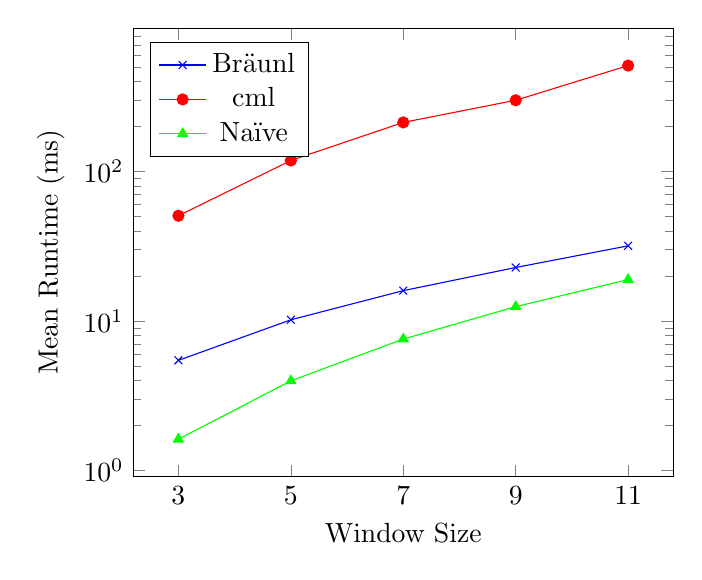
\begin{tikzpicture}
\begin{semilogyaxis}[
	xlabel=Window Size,
    ylabel=Mean Runtime (ms),
    legend pos=north west,
    %xmin=3,
    %xmax=11,
    %minor x tick num=2,
    xtick=data
]
	\addplot [mark=x,blue] table [x=windowSize,y=Mean]{
    	Method	windowSize	filename	Mean	Error	StdDev	Median	Min	Scaled	ScaledSD	Gen0	Gen1	Gen2	Allocated
Bräunl	3	very-small	5.462	0.109	0.285	5.461	4.696	3.37	0.17	31.25	15.625	15.625	2.11
Bräunl	5	very-small	10.195	0.202	0.543	10.087	9.467	2.56	0.14	46.875	31.25	15.625	3.52
Bräunl	7	very-small	15.973	0.318	0.724	15.830	15.012	2.11	0.09	46.875	15.625	-	6.04
Bräunl	9	very-small	22.807	0.447	0.829	22.497	21.855	1.83	0.07	93.75	31.25	-	9.86
Bräunl	11	very-small	31.843	0.621	0.891	31.955	29.750	1.68	0.05	187.5	62.5	-	15.63


    };
    \addplot [mark=*,red] table [x=windowSize,y=Mean]{
    	Method	windowSize	filename	Mean	Error	StdDev	Median	Min	Scaled	ScaledSD	Gen0	Gen1	Gen2	Allocated
\gls{cml}	3	very-small	50.588	2.544	7.500	49.480	40.127	31.18	4.6	166.6667	83.3333	-	1.68
\gls{cml}	5	very-small	118.463	2.349	3.443	119.399	106.345	29.75	0.99	400	200	-	1.69
\gls{cml}	7	very-small	212.817	7.252	21.270	220.862	152.973	28.08	2.79	1000	-	-	1.73
\gls{cml}	9	very-small	299.339	5.264	4.396	298.044	296.011	23.98	0.34	2000	1000	-	1.83
\gls{cml}	11	very-small	510.526	10.065	9.414	510.343	489.584	26.97	0.51	3000	1000	-	1.85

    };
    \addplot [mark=triangle*,green] table [x=windowSize,y=Mean]{
    	Method	windowSize	filename	Mean	Error	StdDev	Median	Min	Scaled	ScaledSD	Gen0	Gen1	Gen2	Allocated
Naïve	3	very-small	1.623	0.003	0.003	1.623	1.618	1	0	154.2969	35.1563	-	2.35
Naïve	5	very-small	3.983	0.076	0.071	3.980	3.891	1	0	382.8125	85.9375	-	5.62
Naïve	7	very-small	7.578	0.011	0.009	7.575	7.566	1	0	734.375	164.0625	-	10.52
Naïve	9	very-small	12.483	0.025	0.022	12.483	12.445	1	0	1171.875	203.125	-	17.26
Naïve	11	very-small	18.933	0.123	0.115	18.896	18.823	1	0	1718.75	187.5	-	23.9
    };
    
    \legend{Bräunl,\gls{cml},Naïve}
\end{semilogyaxis}
\end{tikzpicture}
\caption{\label{graph:median:verysmall}Plot of mean runtimes with a logarithmic y axis for the very small size image}
\end{figure}

%peppers
\begin{figure}
\centering
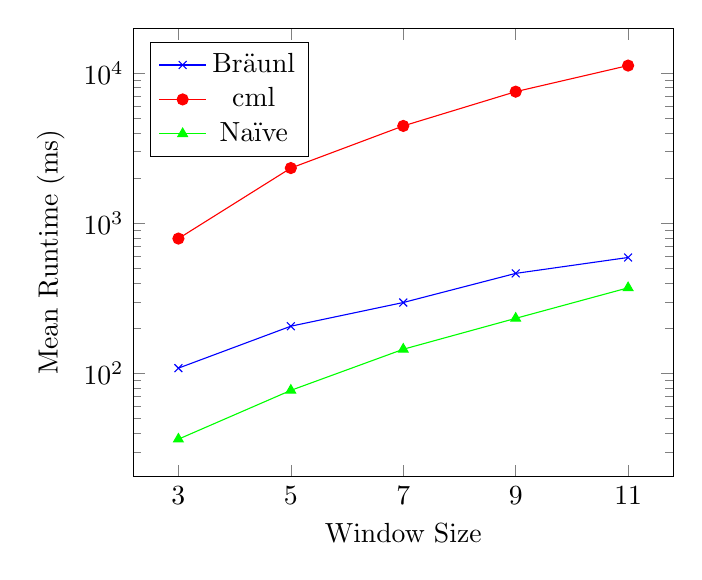
\begin{tikzpicture}
\begin{semilogyaxis}[
	xlabel=Window Size,
    ylabel=Mean Runtime (ms),
    legend pos=north west,
    %xmin=3,
    %xmax=11,
    %minor x tick num=2,
    xtick=data
]
	\addplot [mark=x,blue] table [x=windowSize,y=Mean]{
    	Method	windowSize	filename	Mean	Error	StdDev	Median	Min	Scaled	ScaledSD	Gen0	Gen1	Gen2	Allocated
Bräunl	3	peppers_gray	108.436	2.141	5.088	108.817	93.931	2.98	0.18	1200	1000	1000	37.73
Bräunl	5	peppers_gray	206.336	4.112	9.693	205.430	187.900	2.68	0.15	1000	666.6667	666.6667	58.64
Bräunl	7	peppers_gray	296.717	5.718	5.616	297.432	286.169	2.05	0.12	2000	1000	1000	114.81
Bräunl	9	peppers_gray	463.857	9.138	8.975	464.704	449.199	2	0.13	3000	2000	1000	127.86
Bräunl	11	peppers_gray	592.056	11.749	21.483	589.079	557.281	1.62	0.21	5000	2000	1000	212.34

    };
    \addplot [mark=*,red] table [x=windowSize,y=Mean]{
    	Method	windowSize	filename	Mean	Error	StdDev	Median	Min	Scaled	ScaledSD	Gen0	Gen1	Gen2	Allocated
\gls{cml}	3	peppers_gray	791.285	15.397	23.971	791.190	749.316	21.73	1.09	4000	2000	1000	28.14
\gls{cml}	5	peppers_gray	2333.317	46.639	79.197	2339.807	2108.572	30.29	1.42	8000	3000	2000	28.67
\gls{cml}	7	peppers_gray	4452.903	88.038	183.769	4407.427	4177.586	30.83	2.09	14000	5000	2000	28.28
\gls{cml}	9	peppers_gray	7533.048	150.341	225.023	7527.491	7100.467	32.49	2.2	21000	7000	2000	28.29
\gls{cml}	11	peppers_gray	11237.458	192.938	180.475	11266.773	10925.938	30.74	3.81	32000	10000	4000	29.38
    };
    \addplot [mark=triangle*,green] table [x=windowSize,y=Mean]{
    	Method	windowSize	filename	Mean	Error	StdDev	Median	Min	Scaled	ScaledSD	Gen0	Gen1	Gen2	Allocated
Naïve	3	peppers_gray	36.474	0.724	1.495	36.450	33.341	1	0	3357.1429	1000	1000	36.94
Naïve	5	peppers_gray	77.122	1.532	2.602	77.005	71.833	1	0	7285.7143	1000	1000	87.78
Naïve	7	peppers_gray	144.854	2.895	8.119	142.671	132.158	1	0	13750	1000	1000	175.21
Naïve	9	peppers_gray	232.750	5.198	15.245	227.335	213.438	1	0	21666.6667	1666.6667	1000	239.09
Naïve	11	peppers_gray	371.789	17.122	50.485	345.788	313.159	1	0	32000	1000	1000	337.86
    };
    
    \legend{Bräunl,\gls{cml},Naïve}
\end{semilogyaxis}
\end{tikzpicture}
\caption{\label{graph:median:peppers}Plot of mean runtimes with a logarithmic y axis for the peppers image}
\end{figure}

%small
\begin{figure}
\centering
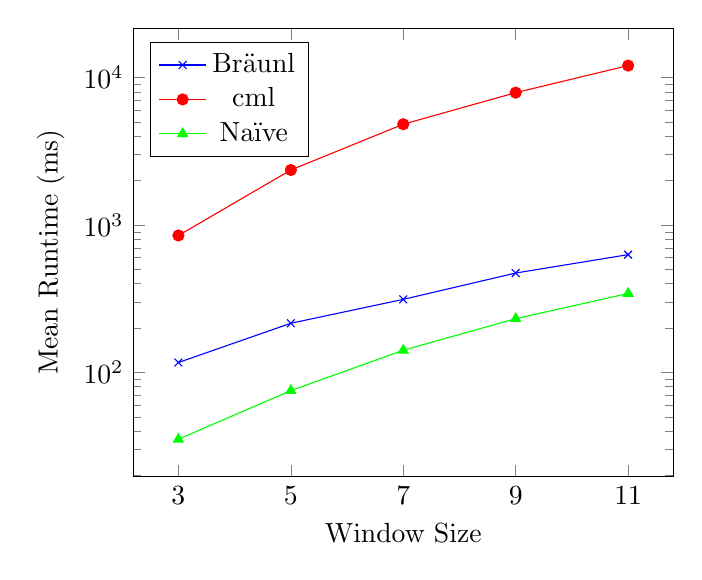
\begin{tikzpicture}
\begin{semilogyaxis}[
	xlabel=Window Size,
    ylabel=Mean Runtime (ms),
    legend pos=north west,
    %xmin=3,
    %xmax=11,
    %minor x tick num=2,
    xtick=data
]
	\addplot [mark=x,blue] table [x=windowSize,y=Mean]{
    	Method	windowSize	filename	Mean	Error	StdDev	Median	Min	Scaled	ScaledSD	Gen0	Gen1	Gen2	Allocated
Bräunl	3	small	116.782	2.334	4.208	116.874	107.437	3.32	0.14	1200	1000	800	40.96
Bräunl	5	small	215.573	4.295	12.185	217.475	180.880	2.86	0.16	1666.6667	1333.3333	1000	63.03
Bräunl	7	small	313.114	2.952	2.761	312.674	309.410	2.21	0.02	2000	1000	1000	111.37
Bräunl	9	small	472.517	4.680	4.378	473.456	460.456	2.04	0.02	4000	2000	1000	161.63
Bräunl	11	small	629.898	5.558	4.927	628.729	618.231	1.83	0.02	5000	2000	1000	149.05

    };
    \addplot [mark=*,red] table [x=windowSize,y=Mean]{
    	Method	windowSize	filename	Mean	Error	StdDev	Median	Min	Scaled	ScaledSD	Gen0	Gen1	Gen2	Allocated
\gls{cml}	3	small	849.482	19.570	56.149	828.209	773.390	24.12	1.69	4000	2000	1000	33.68
\gls{cml}	5	small	2362.643	46.461	104.871	2355.982	2162.910	31.39	1.39	9000	3000	2000	33.25
\gls{cml}	7	small	4830.294	95.856	137.474	4834.632	4523.971	34.15	0.97	14000	5000	2000	33.04
\gls{cml}	9	small	7910.925	134.530	125.839	7909.106	7701.102	34.15	0.54	23000	8000	3000	34.13
\gls{cml}	11	small	12074.170	232.388	228.236	12042.342	11712.425	35.17	0.66	32000	11000	3000	34

    };
    \addplot [mark=triangle*,green] table [x=windowSize,y=Mean]{
    	Method	windowSize	filename	Mean	Error	StdDev	Median	Min	Scaled	ScaledSD	Gen0	Gen1	Gen2	Allocated
Naïve	3	small	35.246	0.697	0.881	34.905	34.267	1	0	3466.6667	1000	1000	37.65
Naïve	5	small	75.282	0.506	0.473	75.217	74.419	1	0	7857.1429	1000	1000	95.36
Naïve	7	small	141.432	0.804	0.752	141.446	140.203	1	0	14000	1000	1000	175.74
Naïve	9	small	231.667	0.979	0.867	232.029	229.561	1	0	22666.6667	1666.6667	1000	328.08
Naïve	11	small	343.286	1.710	1.600	342.643	341.541	1	0	33000	1000	1000	261.29
    };
    
    \legend{Bräunl,\gls{cml},Naïve}
\end{semilogyaxis}
\end{tikzpicture}
\caption{\label{graph:median:small}Plot of mean runtimes with a logarithmic y axis for the small size image}
\end{figure}

\begin{anfxerror}
Really need to change these charts to use a log scale on the y axis.  It'll make it much easier to see the relative changes.
\end{anfxerror}

%medium
\begin{figure}
\centering
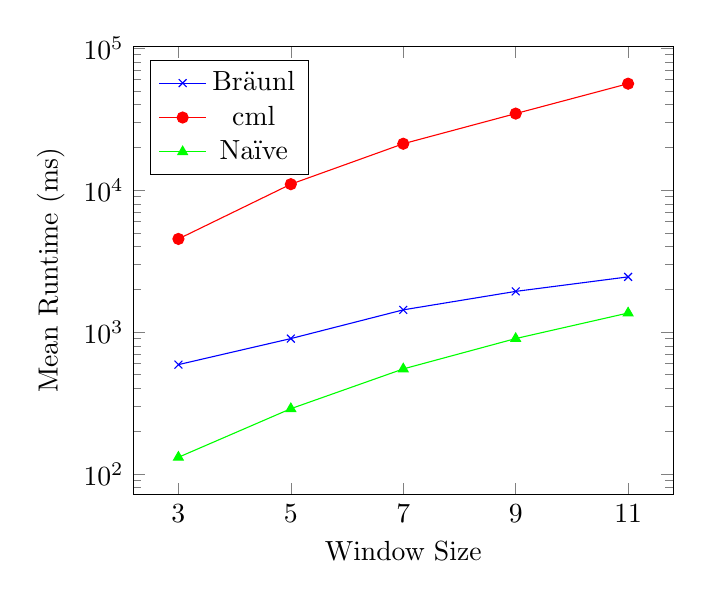
\begin{tikzpicture}
\begin{semilogyaxis}[
	xlabel=Window Size,
    ylabel=Mean Runtime (ms),
    legend pos=north west,
    %xmin=3,
    %xmax=11,
    %minor x tick num=2,
    xtick=data
]
	\addplot [mark=x,blue] table [x=windowSize,y=Mean]{
    	Method	windowSize	filename	Mean	Error	StdDev	Median	Min	Scaled	ScaledSD	Gen0	Gen1	Gen2	Allocated
Bräunl	3	medium	589.431	11.668	10.344	585.135	574.774	4.51	0.27	2000	1000	1000	146.49
Bräunl	5	medium	899.233	4.445	3.940	899.270	892.109	3.12	0.07	4000	2000	1000	230.3
Bräunl	7	medium	1433.220	31.164	29.151	1431.262	1379.761	2.61	0.07	7000	4000	2000	374.04
Bräunl	9	medium	1933.758	24.222	22.657	1925.642	1905.768	2.15	0.02	16000	4000	2000	527.35
Bräunl	11	medium	2447.284	47.271	50.580	2451.473	2352.536	1.8	0.05	40000	4000	2000	167.19

    };
    \addplot [mark=*,red] table [x=windowSize,y=Mean]{
    	Method	windowSize	filename	Mean	Error	StdDev	Median	Min	Scaled	ScaledSD	Gen0	Gen1	Gen2	Allocated
\gls{cml}	3	medium	4527.962	89.754	226.819	4511.961	4003.316	34.65	2.61	12000	6000	3000	132.41
\gls{cml}	5	medium	11006.775	197.445	184.691	10983.829	10737.131	38.19	1.05	28000	10000	4000	138.84
\gls{cml}	7	medium	21210.296	417.303	409.847	21118.240	20410.160	38.61	1.08	50000	15000	4000	136.78
\gls{cml}	9	medium	34587.347	471.655	441.186	34687.611	33898.247	38.45	0.48	81000	22000	4000	137.63
\gls{cml}	11	medium	56196.611	1118.853	2548.193	55158.372	52956.449	41.29	2.05	230000	66000	4000	132.75
    };
    \addplot [mark=triangle*,green] table [x=windowSize,y=Mean]{
    	Method	windowSize	filename	Mean	Error	StdDev	Median	Min	Scaled	ScaledSD	Gen0	Gen1	Gen2	Allocated
Naïve	3	medium	131.111	2.655	7.787	128.188	122.294	1	0	11500	1500	1500	102.34
Naïve	5	medium	288.343	5.716	6.805	285.656	282.623	1	0	28000	1000	1000	371.43
Naïve	7	medium	549.600	12.951	12.114	543.465	539.418	1	0	54000	1000	1000	710.4
Naïve	9	medium	899.563	3.131	2.444	900.523	893.992	1	0	89000	2000	1000	985.29
Naïve	11	medium	1361.629	27.108	31.217	1350.193	1344.088	1	0	131000	4000	1000	1969.78
    };
    
    \legend{Bräunl,\gls{cml},Naïve}
\end{semilogyaxis}
\end{tikzpicture}
\caption{\label{graph:median:medium}Plot of mean runtimes with a logarithmic y axis for the medium size image}
\end{figure}

%\gls{cml}
\begin{figure}
\centering
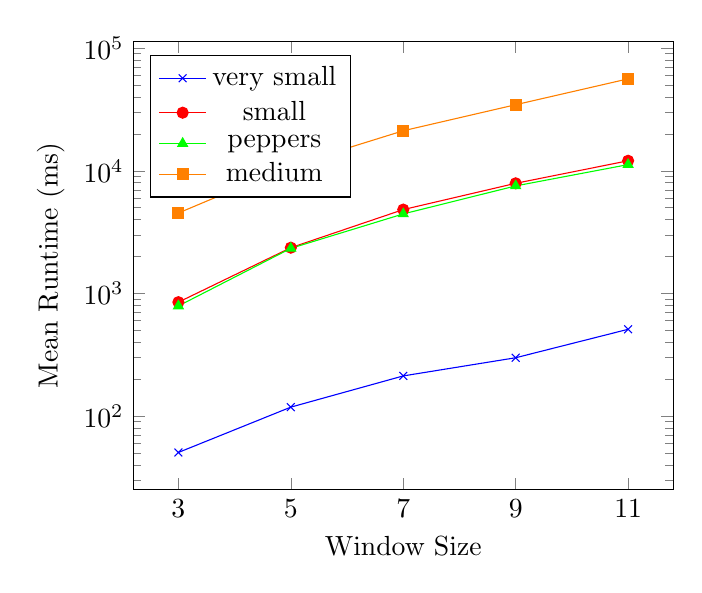
\begin{tikzpicture}
\begin{semilogyaxis}[
	xlabel=Window Size,
    ylabel=Mean Runtime (ms),
    legend pos=north west,
    %xmin=3,
    %xmax=11,
    %minor x tick num=2,
    xtick=data
]
	\addplot [mark=x,blue] table [x=windowSize,y=Mean]{
    	Method	windowSize	filename	Mean	Error	StdDev	Median	Min	Scaled	ScaledSD	Gen0	Gen1	Gen2	Allocated
\gls{cml}	3	very-small	50.588	2.544	7.500	49.480	40.127	31.18	4.6	166.6667	83.3333	-	1.68
\gls{cml}	5	very-small	118.463	2.349	3.443	119.399	106.345	29.75	0.99	400	200	-	1.69
\gls{cml}	7	very-small	212.817	7.252	21.270	220.862	152.973	28.08	2.79	1000	-	-	1.73
\gls{cml}	9	very-small	299.339	5.264	4.396	298.044	296.011	23.98	0.34	2000	1000	-	1.83
\gls{cml}	11	very-small	510.526	10.065	9.414	510.343	489.584	26.97	0.51	3000	1000	-	1.85


    };
    \addplot [mark=*,red] table [x=windowSize,y=Mean]{
    	Method	windowSize	filename	Mean	Error	StdDev	Median	Min	Scaled	ScaledSD	Gen0	Gen1	Gen2	Allocated
\gls{cml}	3	small	849.482	19.570	56.149	828.209	773.390	24.12	1.69	4000	2000	1000	33.68
\gls{cml}	5	small	2362.643	46.461	104.871	2355.982	2162.910	31.39	1.39	9000	3000	2000	33.25
\gls{cml}	7	small	4830.294	95.856	137.474	4834.632	4523.971	34.15	0.97	14000	5000	2000	33.04
\gls{cml}	9	small	7910.925	134.530	125.839	7909.106	7701.102	34.15	0.54	23000	8000	3000	34.13
\gls{cml}	11	small	12074.170	232.388	228.236	12042.342	11712.425	35.17	0.66	32000	11000	3000	34

    };
    \addplot [mark=triangle*,green] table [x=windowSize,y=Mean]{
    	Method	windowSize	filename	Mean	Error	StdDev	Median	Min	Scaled	ScaledSD	Gen0	Gen1	Gen2	Allocated
\gls{cml}	3	peppers_gray	791.285	15.397	23.971	791.190	749.316	21.73	1.09	4000	2000	1000	28.14
\gls{cml}	5	peppers_gray	2333.317	46.639	79.197	2339.807	2108.572	30.29	1.42	8000	3000	2000	28.67
\gls{cml}	7	peppers_gray	4452.903	88.038	183.769	4407.427	4177.586	30.83	2.09	14000	5000	2000	28.28
\gls{cml}	9	peppers_gray	7533.048	150.341	225.023	7527.491	7100.467	32.49	2.2	21000	7000	2000	28.29
\gls{cml}	11	peppers_gray	11237.458	192.938	180.475	11266.773	10925.938	30.74	3.81	32000	10000	4000	29.38
    };
    \addplot [mark=square*,orange] table [x=windowSize,y=Mean]{
    	Method	windowSize	filename	Mean	Error	StdDev	Median	Min	Scaled	ScaledSD	Gen0	Gen1	Gen2	Allocated
\gls{cml}	3	medium	4527.962	89.754	226.819	4511.961	4003.316	34.65	2.61	12000	6000	3000	132.41
\gls{cml}	5	medium	11006.775	197.445	184.691	10983.829	10737.131	38.19	1.05	28000	10000	4000	138.84
\gls{cml}	7	medium	21210.296	417.303	409.847	21118.240	20410.160	38.61	1.08	50000	15000	4000	136.78
\gls{cml}	9	medium	34587.347	471.655	441.186	34687.611	33898.247	38.45	0.48	81000	22000	4000	137.63
\gls{cml}	11	medium	56196.611	1118.853	2548.193	55158.372	52956.449	41.29	2.05	230000	66000	4000	132.75
    };
    
    \legend{very small,small,peppers,medium}
\end{semilogyaxis}
\end{tikzpicture}
\caption[Plot of mean runtimes for the \glsentrylong{cml-glossary} algorithm on different image sizes]{\label{graph:median:cmls}Plot of mean runtimes with a logarithmic y axis for the \gls{cml} algorithm on different image sizes}
\end{figure}

\begin{figure*}
\subfloat[]{\includegraphics[width=0.2\textwidth]{chapters/medianfilter/images/peppers/peppers_gray.png}}
\subfloat[]{\includegraphics[width=0.2\textwidth]{chapters/medianfilter/images/peppers/peppers_gray_noisy.png}}
\subfloat[]{\includegraphics[width=0.2\textwidth]{chapters/medianfilter/images/peppers/naive_peppers_gray_noisy_3.png}}
\subfloat[]{\includegraphics[width=0.2\textwidth]{chapters/medianfilter/images/peppers/braunl_peppers_gray_noisy_3.png}}
\subfloat[]{\includegraphics[width=0.2\textwidth]{chapters/medianfilter/images/peppers/cml_peppers_gray_noisy_3.png}}
\caption[The classic grayscale `peppers' image, before and after processing]{\label{fig:median:peppers}The classic grayscale `peppers' image, before and after processing.  (a) is the original image; (b) is the image with random salt \& pepper noise introduced; (c) is the result of processing the image using the naïve algorithm; (d) is the result of processing the image using the Br\"{a}unl-inspired algorithm; (e) is the result of processing the image using the \gls{cml} algorithm}
\end{figure*}

\begin{table}
\centering
\caption[Peak signal-to-noise for the very small image]{Peak signal-to-noise ratio measurement for the very small image (measured in dB)}
\label{tab:median:psnrvsmall}
\begin{tabular}{@{}lccccc@{}}
\toprule
\multicolumn{1}{c}{\textbf{Algorithm}} & \multicolumn{5}{c}{\textbf{Window size}}                                          \\
                                       & 3              & 5              & 7              & 9             & 11             \\ \midrule
Bräunl                                 & 20.78          & 17.82          & 15.65          & 14.36         & 13.55          \\
\gls{cml}                                    & 25.98          & \textbf{21.85} & \textbf{18.62} & \textbf{16.40} & 14.99          \\
Naïve                                  & \textbf{27.03} & 21.74          & 18.55          & 16.39         & \textbf{15.02} \\ \bottomrule
\end{tabular}
\end{table}

\begin{table}
\centering
\caption[Peak signal-to-noise for the peppers image]{Peak signal-to-noise ratio measurement for the peppers image (measured in dB)}
\begin{tabular}{@{}lccccc@{}}
\toprule
\multicolumn{1}{c}{\textbf{Algorithm}} & \multicolumn{5}{c}{\textbf{Window size}}                                          \\
                                       & 3              & 5              & 7              & 9              & 11            \\ \midrule
Bräunl                                 & 28.76          & 27.35          & 25.27          & 23.94          & 22.82         \\
\gls{cml}                                    & 31.85          & 31.07          & 29.8           & 28.56          & 27.42         \\
Naïve                                  & \textbf{32.79} & \textbf{31.25} & \textbf{29.87} & \textbf{28.63} & \textbf{27.50} \\ \bottomrule
\end{tabular}
\label{tab:median:psnrpeppers}
\end{table}

\begin{table}
\centering
\caption[Peak signal-to-noise for the small image]{Peak signal-to-noise ratio measurement for the small image (measured in dB)}
\label{tab:median:psnrsmall}
\begin{tabular}{@{}lccccc@{}}
\toprule
\multicolumn{1}{c}{\textbf{Algorithm}} & \multicolumn{5}{c}{\textbf{Window size}}                                          \\
                                       & 3              & 5              & 7             & 9              & 11             \\ \midrule
Bräunl                                 & 32.83          & 32.34          & 30.74         & 29.73          & 28.94          \\
\gls{cml}                                    & 36.62          & 34.25          & 32.66         & 31.57          & 30.71          \\
Naïve                                  & \textbf{37.83} & \textbf{34.31} & \textbf{32.7} & \textbf{31.65} & \textbf{30.81} \\ \bottomrule
\end{tabular}
\end{table}

\begin{table}
\centering
\caption[Peak signal-to-noise for the medium image]{Peak signal-to-noise ratio measurement for the medium image (measured in dB)}
\begin{tabular}{@{}lccccc@{}}
\toprule
\multicolumn{1}{c}{\textbf{Algorithm}} & \multicolumn{5}{c}{\textbf{Window size}}                                           \\
                                       & 3              & 5              & 7              & 9              & 11             \\ \midrule
Bräunl                                 & 32.98          & 32.65          & 31.59          & 30.91          & 30.36          \\
\gls{cml}                                    & 36.72          & \textbf{34.15} & \textbf{32.98} & \textbf{32.26} & \textbf{31.73} \\
Naïve                                  & \textbf{37.16} & 34.07          & 32.96          & \textbf{32.26} & \textbf{31.73} \\ \bottomrule
\end{tabular}
\label{tab:median:psnrmedium}
\end{table}

Examination of the reported memory statistics (please see the GitHub repository for details) appears to show that the maximum amount of memory allocated during processing for the \gls{cml} algorithm stays roughly constant across window sizes for each image size, and in fact on larger window sizes it is the most memory efficient.  The naïve algorithm quickly grows to consume the most memory at larger window sizes for each image size, suggesting that it likely derives some of its comparative speed at the cost of greater space complexity, while Bräunl sits in the middle.  Conversely, \gls{cml} generates by far the most garbage collection events, which may help explain its relative lack of pace.

\section{Discussion}
%These algorithms are not necessarily the best for performing this operation, as they ignore the potential for taking advantage of data-parallelism.

The algorithms developed and presented here are not necessarily optimal for the purpose.  They largely handle each pixel separately, or combine them into arrays on-the-fly.  This ignores the possibility of exploiting data-parallelism to improve throughput, and instead relies only on the separate CPU cores to provide the parallelism.

It is unclear how much the mechanics underlying these implementations (i.e. the .NET Core and \hopac{} systems) attempt to maximise use of the processor cache.  Efficient use of the cache can contribute significantly to an optimised version of an algorithm outperforming a simplistic version by an order of magnitude or more \cite{Ragan-Kelley2017}.  No attempt was made manually to ensure good practices such as tiling or striping.  %Differences in cache exploitation may also go some way to explaining differences in execution time.

The \gls{cml} approach used essentially instantiates a separate logical processing element for each pixel, each of which must be scheduled to run at some point -- concurrent with another one in the case of synchronous message passing.  It is possible that this surfeit of separate logical threads may induce excessive switching costs, and perhaps promote wasted time with threads spending time polling their channel and their neighbours'.  Careful improvements to this and the use of the cache might lead to significant gains in speed.

In terms of the code itself also, \gls{cml} appears to be the worst.  The program requires roughly double the number of lines of the naïve program, and is arguably much less `clean' or `readable'.  Reinterpreting the \gls{medianfilter} in terms of synchronously communicating processes has not yielded a structural improvement nor simplified the programming task.  Combined with the running time results above, this suggests that the \gls{cml} approach is actively unhelpful for implementing \glspl{mwt}, at least when using \hopac{}.

Basic profiling of the \gls{cml}-based implementation appears to show that more than half of the runtime of the program was spent inside the function for giving a value over a channel, and functions called by it.  Furthermore, according to this profiling, almost 40\% of the total running time of the algorithm is taken up specifically by low-level memory management functions inside the depths of the .NET Core system.  Considering that some of these functions are written in hand-optimised assembly \fxwarning[inline]{ref?}, the fact they account for so much of the running time appears to suggest that memory use is poorly handled in the tested implementation.

\Glspl{mwt} are generally relatively simplistic processes, which typically consist simply of combining values from the pixel array, which can be programmed in a straightforward fashion.  More sophisticated programming techniques may simply `get in the way' and introduce unnecessary overheads, which appears to have happened here.  Furthermore, the \gls{medianfilter} can largely be broken down into arithmetic and logical operations amenable to vectorisation (e.g. \cite{Sanchez2012,Perreault2007}), which the \gls{cml} approach currently ignores entirely.

\subsection{Threats to validity}
There are two identifiable threats to validity, both regarding the `quality' of the programming involved.  .NET Core, as a widely used open source compiler and runtime system which has likely had millions of man-hours invested in it, is presumably of high quality and fast in most cases.  That is not necessarily the case with \hopac{}.  While it is open source, and moderately well-known in the \fsharp{} community, the amount of time spent on optimising it is likely nowhere close to that spent on .NET Core.  This means that \hopac{} itself may present significant bottlenecks while performing the \gls{mwt}.  While it is reasonable to expect that `give' operations would be a large part of the total running time, as a central part of the operation of the algorithm, it is surprising to see it take more than 50\% of the time.

The other threat to validity is the skill of the end programmer.  The author was new to the \hopac{} library at the start of this work, and inferior design choices may have been made unwittingly.  It was, however, suggested during personal communication with one of the maintainers and fellow users of the \hopac{} library that the \gls{cml} approach may simply be a poor fit to pixel-wise image processing tasks.

Fundamentally, the results achieved here, as with most implementation exercises, succeed or fail in large part on the skill, knowledge and effort of the programmers involved.  The use of other libraries may lead to better results.  Other relatively recent implementations of \gls{cml} exist, such as Concurrent Haskell \cite{Chaudhuri2009} and Fibers\footnote{\url{https://github.com/wingo/fibers}} for Guile Scheme, but a lack of time meant that they could not yet be assessed further.

\section{Conclusion}
The use of a \gls{cml} approach to image processing was explored in this work, in particular as applied to the \gls{medianfilter} \gls{mwt} operation.  The measured results suggest that it is much worse than using a simple, naïve nested-for-loops approach.  The reason for this appears to be primarily related to overhead from the synchronous communications, especially in regard to memory allocations and garbage collections.  This may be an issue with the \gls{cml} style in general, \fxerror{That ended up looking like it was at least partially true.}{or it may be an issue related to the \gls{cml} library used} or the programming of the algorithms tested here.  More work is required to determine this for certain.  \gls{cml} does appear to provide one advantage, however, in that for larger window sizes it seemingly has the lowest peak space requirement.

A \gls{cml} approach where a separate logical processing element is used to represent each pixel largely eliminates the possibility of taking advantage of data-parallel hardware, such as vector instructions of CPUs or \glspl{gpu}.  For situations where vector instructions are applicable, the \gls{cml} approach seems likely to be a poor choice.  It is not clear, however, how well this approach may or may not work for instances where the data types involved are more complex, or where there is a significant level of control flow involved.

% Future work should explore \gls{cml} as applied to other computer vision algorithms, especially those which can naturally be characterised in terms of message passing, or which use more complex data types.  Other \gls{cml} implementations beyond the one used here should be tested too, as it is not clear how much the problems experienced by this \gls{cml} program may stem from the implementation of the \gls{cml} library used.
\glsresetall
\cpresetrulenumber
\chapter{Discussion}

Where I discuss the good \& bad about this work

% \section{Comparison of \glsentrylong{mpbsm} algorithms}

% What am I comparing them to?  Algos coded by myself?  The best I can find out there of others'?

% \subsection{\glsentrylong{bp}}

% \subsection{\glsentrylong{cp}}

\section{Limitations}

\subsection{Threats to Validity}

\section{Alternatives for Investigation}

\subsection{Other languages \& libraries}
Implement my own version of \gls{cml} in Rust or Julia, etc?  Looks like Felix has most if not all of the necessary components for it.

\subsection{Other Computational Models}
Actors, Join Calculus, Pi Calculus

\subsection{Potentially Useful Hardware}

\subsubsection{CPU Additions}
Intel's Transactional Synchronisation Extensions (TSX) -- \url{https://en.wikipedia.org/wiki/Transactional_Synchronization_Extensions}

AMD's Advanced Synchronization Facility (ASF) -- \url{https://en.wikipedia.org/wiki/Advanced_Synchronization_Facility}

mEDA (modified Extended Dataflow Actor) \& full/empty memory tagging (F/E bits?) e.g. \url{https://link.springer.com/chapter/10.1007/BFb0057916} \& \url{https://people.kth.se/~vladv/abstracts/TRITA-IT-0004.pdf}

\subsubsection{Is Hyper-Threading Helpful?}

\subsubsection{GPUs?}

\glsresetall
\cpresetrulenumber
\chapter{Conclusion}

I did some stuff!

\section{Future Directions}

\begin{anfxwarning}{Where should this go?}
    Similar material is also covered in the discussion chapter.  Should much of the below be shifted into there?  Alternatively, should much of the stuff from the discussion chapter move to here?
\end{anfxwarning}

% The use of Full/Empty bits looks highly promising for making message passing more efficient.  It doesn't seem to have any real support in mainstream/commodity hardware, however.  There were Intel's TGX instructions, but they have been taken out of processors again.

% Extended Dataflow Actors?  Or is it Extended Dataflow Architecture?

% \fxerror*{Not entirely sure BSP is relevant here}{See also the Bulk Synchronous Parallel approach.}

% https://scholar.google.co.nz/scholar?q=related:Z8GZl-HQcSkJ:scholar.google.com/&scioq=A+Static+Mapping+System+for+Logically+Shared+Memory+Parallel+Programs&hl=en&as_sdt=0,5&inst=15360723290749679499

% http://citeseerx.ist.psu.edu/viewdoc/download?doi=10.1.1.50.8739&rep=rep1&type=pdf

% https://link.springer.com/chapter/10.1007/BFb0057916

% https://link.springer.com/chapter/10.1007/3-540-63697-8_82

None of the below were investigated further, due to a lack of time, but they are obvious next steps to look at.

% \subsection{\glsentrytext{cml}}
% \Gls{cml} seems like the obvious approach to take from here.\footnote{In fact, considerable time and effort was spent on attempting to identify a suitable \gls{cml} implementation to use for just this purpose.  Unfortunately, in the end, it was found that there was not currently a usable \gls{cml} implementation with appropriate performance available at this time.}

% \subsection{`Faked' message passing in shared memory}
% Roughly, most of the message passing involved here is largely, in effect, just handing around pointers to memory locations.  It would seem that the message passing itself places some overhead in the way of that.  Could there be some way to fake the message passing, so that to the program's writer it looks like an actual message passing implementation, but in reality it is just doing normal updates on mutable memory?  This \emph{might} enable the best of both worlds -- programming the algorithms according to their theory, but running in a highly efficient fashion `under-the-hood'.

% It is not too clear how to achieve this (if it is indeed possible), but Rust would appear to be a good language to target for it.  Rust is fairly high-performance by default and enables quite a lot of low-level memory manipulation.  Moreover, its move semantics pretty much fit exactly to the concepts used here, and, on the face of it, its macro system would appear to be a convenient way to abstract over many of the details and provide a message passing façade, while actually doing efficient operations behind that.

% It looks like the C++ \texttt{mess} library is intended to be exactly this sort of thing:  \url{https://github.com/LouisCharlesC/mess}.  The developer seems to say that the user gets to write their program in a message-passing fashion, but mess does some clever meta-programming so that there ends up being zero overhead in the end.  Also, absolutely \emph{must} address Halide, and explain why it wasn't pursued here.  Otherwise, that'll be the elephant in the room.

% \subsection{Other hardware}
% This work focused on CPU-based systems, largely excluding other hardware.  If used well, all three of \glspl{gpu}, \glspl{fpga} and \glspl{dsp} have potential to perform vastly more computations per second, suggesting that a high-performance message passing-based system would do well to use them.  In each case, however, they do not work in quite the same way as CPUs, meaning that programming them is not necessarily straightforward, especially when trying to achieve a programming style that differs to their default.  As described in \fxwarning*{insert the appropriate cross-reference}{the literature review chapter}, fast \gls{gpu} implementations of \gls{bp} have been created, suggesting that message passing on a \gls{gpu} is entirely plausible.

% It would appear worthwhile to investigate how one might be able to implement some sort of message passing system atop these hardware alternatives, due to the potential for many more computations per second.  Even better would be to create a heterogeneous system which can take full advantage of the strengths of each hardware type, while overcoming its weaknesses.  Precisely how to achieve efficient implementations on them is unknown.  The fact that OpenCL \fxerror[inline]{[ref]} (and, to some extent at least, OpenACC \fxerror[inline]{[ref]}) can be compiled from the same base code to different devices makes it an obvious starting point.   There has already been at least one publication on implementing \glspl{actor} in OpenCL \fxerror[inline]{[ref]}, suggesting it is possible -- though how well synchronous message passing will work as compared to asynchronous remains to be seen.

% See also \url{https://hastlayer.com/} -- they seem to say that they do relevant stuff on FPGAs.  Interestingly, they also do unums/posits, apparently.

\subsection{Universal Numbers}
The \gls{cps} work kinda ignored non-integer numbers, which in real practice is quite a glaring omission.  Investigating modelling IEEE-754 floating point (and/or the fixed-point version), as well as Gufstafson's unums/posits, would be another good step to take.

%%%%%%%%%%%%%%%%%%%%%%%%%%%%%%%%%%%%%%%%%%%%%%%%%%%%%%%%%%%%%%%%%%%%%%%%%%%%%%%%%

\subsection{\nameref{chap:tsp}}
One-way multiset unification occurs frequently in \gls{cps}, with unification being used in every rule presented above.  \fxerror*{Isn't this what Yezhou's paper \cite{Liu2021} covers?}{An efficient algorithm to perform this task would be highly beneficial for creating useful simulations of systems (we are not aware of an efficient algorithm in the case of multisets).}  For example, our simulations of the \gls{tsp} algorithm written in functional programming languages (see \cref{sec:tsp:simulation}) regularly simply iterate over all relevant objects in the system, even though frequently most will be of little use in a given function call, and so the simulations could benefit from improved unification in practice.

We would like to further develop the capacity to simulate \gls{cps}, in particular developing more advanced techniques for translating \gls{cps} rules to efficient parallel code.  Work down this avenue has not begun as yet, however.

%%%%%%%%%%%%%%%%%%%%%%%%%%%%%%%%%%%%%%%%%%%%%%%%%%%%%%%%%%%%%%%%%%%%%%%%%%%%%%%%%

\subsection{\nameref{chap:median}}

The median filter algorithm investigated was pretty much the most basic one possible.  The experiment should be extended to cover more complicated algorithms that perform better at reconstructing the image.  These may be better suited to a message-passing approach compared to a na\"ive one than the basic method.

Future work should explore \gls{cml} as applied to other computer vision algorithms, especially those which can naturally be characterised in terms of message passing, or which use more complex data types.  Other \gls{cml} implementations beyond the one used here should be tested too, as it is not clear how much the problems experienced by this \gls{cml} program may stem from the implementation of the \gls{cml} library used.

%%%%%%%%%%%%%%%%%%%%%%%%%%%%%%%%%%%%%%%%%%%%%%%%%%%%%%%%%%%%%%%%%%%%%%%%%%%%%%%%%

\subsection{\nameref{chap:nmp}}
The next step in this work is to adapt the system to the purpose of Belief Propagation Stereo Matching, using \gls{nmp} precepts.  This will be presented in Part Two.  Furthermore, work has begun on implementing a close approximation of the asynchronous system as a framework in a standard programming languages, to explore the effectiveness of this approach in modern computer systems.  We plan to implement Belief Propagation Stereo Matching (see e.g. \cite{Blake2011,Felzenszwalb2011,JianSun2003}) atop this as a proof-of-concept.

One aspect the systems presented above lack is that both the size and shape of the grid involved, as well as the communication topology between neighbours, are permanently fixed at the time of system initialisation.  In most cases, this is unneeded, but the greater flexibility could be of use when implementing certain algorithms.

Furthermore, at present, it is implicitly assumed that every \gls{pe} remains active throughout the entirety of the system's evolution until it has sent and received all of its scheduled messages.  Within the context of \gls{cps} this is largely irrelevant, but permitting \glspl{pe} to deactivate at appropriate points could save processing power in other circumstances with bounded parallelism.  Complicating this is ensuring that those \glspl{pe} which do remain active can continue messaging as needed despite one or more neighbours deactivating.

We also have yet to examine the systems with respect to communication complexity measures such as those found in \cite{Juayong2020}.  The precise results presented there are not directly applicable to this work, given the use of different P~systems models, but the underlying concepts appear directly relevant.

%%%%%%%%%%%%%%%%%%%%%%%%%%%%%%%%%%%%%%%%%%%%%%%%%%%%%%%%%%%%%%%%%%%%%%%%%%%%%%%%%

% ====================================================
%
% ENDMATTER
%
% Appendices and bibliography 
% Pagination arabic, re-starts at 1
%
% ====================================================

\cleardoublepage % start afresh on a new page
\setcounter{page}{1} % re-sets the page counter

\printbibliography[title={Works Cited}, heading=bibintoc]

\printglossary
 
\printglossary[type=\acronymtype]

% \cleardoublepage
% Put an index here?

% \cleardoublepage % start afresh on a new page
% \setcounter{page}{1} % re-sets the page counter
% \appendixpage* % makes a page to mark beginning of appendices -- currently there are no appendices
% \input{appendix1} 


\end{document}